\documentclass[a5paper,twoside]{book}
\usepackage[left=1.5cm,right=1.7cm,top=1.5cm,bottom=1.5cm]{geometry}

\usepackage{Labnik}
\usepackage{Labnik-III-shortcuts}

%\renewcommand{\todo}[1]{}

% для таблиц
\usepackage{tabularx}
\usepackage{multirow}
\usepackage{bigstrut}
\usepackage{dcolumn}

% увеличить страницу
\newcommand{\etp}[1]{\enlargethispage*{#1\baselineskip}}

\def\tom{2}
\def\nazvan{Электричество и магнетизм}
\def\god{2019}

\AtEndDocument{\label{book:last-page}}

\begin{document}

%Обложка
%===========================
\setcounter{page}{1}
\thispagestyle{empty}\mbox{}

\noindent
\raisebox{0mm}{
\includegraphics[width=25mm]{gerb}}%
\hfill
\parbox{90mm}{\centering\itshape Московский физико-технический институт\par
(национальный исследовательский университет)\par}%
\hfill

\vfill

{\parindent=0pt\centering
{\noindent\bfseries\Huge ЛАБОРАТОРНЫЙ\strut\\ ПРАКТИКУМ\strut\\
}
{\bfseries\LARGE ПО ОБЩЕЙ ФИЗИКЕ }

\vfill

%{\bfseries\large ТОМ \tom\strut}

%\medskip

{\bfseries\large\strut ЭЛЕКТРИЧЕСТВО И МАГНЕТИЗМ\strut}

}

\newlength{\vva}
\setlength{\vva}{0.3\textwidth}
\newlength{\vvb} 
\setlength{\vvb}{0.46\textwidth}

\vfill

%todo Сделать картинку на обложку

{\hfil Версия: \today}

%\noindent\mbox{}\hfil
%\hbox to \vva{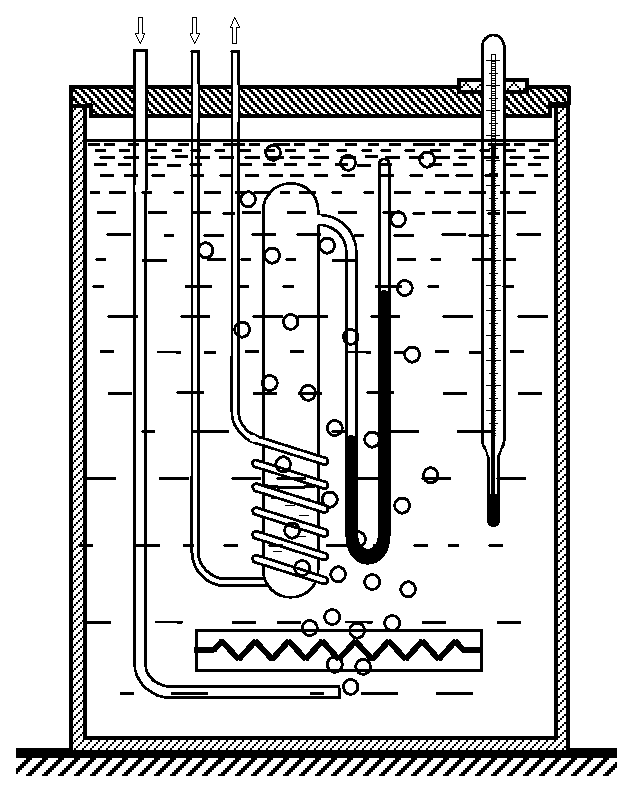
\includegraphics[width=\vva]{pic/O1}}%
%\hfil
%\hbox to \vvb{\includegraphics[width=\vvb]{pic/O2}}%

\vfill

\newpage

\setcounter{page}{1}
\thispagestyle{empty}\mbox{}
%\vskip5mm

\begingroup
\parindent=0pt\centering
{\scriptsize
Министерство науки и высшего образования Российской Федерации\\
Федеральное государственное автономное\\
образовательное учреждение высшего образования\\
<<Московский физико-технический институт\\ 
(национальный исследовательский университет)>>\par
}

\vskip 20mm

{\bfseries\LARGE\strut ЛАБОРАТОРНЫЙ\strut\\ ПРАКТИКУМ\strut\\ ПО ОБЩЕЙ ФИЗИКЕ\strut}

\vskip 10mm

{\bfseries\Large В трёх томах}

\vskip 10mm

{\bfseries\Large Том 2}

\vskip 5mm

{\bfseries\Large \MakeUppercase{\nazvan}}

\vskip 5mm

Издание второе, переработанное и дополненное

\vskip 20mm

%{\it\small Рекомендовано\\ Учебно-методическим объединением\\
%высших учебных заведений Российской Федерации\\
%по образованию в области прикладных математики и физики\\
%в качестве учебного пособия для студентов вузов\\
%по направлению подготовки <<Прикладные математика и физика>> }

\vskip 10mm

{\bfseries Под редакцией\strut\\
% проф. А.Д.~ГЛАДУНА\strut}
проф. А.\,В.~МАКСИМЫЧЕВА и проф. М.\,Г.~НИКУЛИНА\strut}

\vfill

{\small МОСКВА\\
МФТИ\\
\god}\par
\endgroup

\newpage

\setcounter{page}{2}

\thispagestyle{empty}

{\parindent=0pt {\footnotesize
УДК 53(075)\\
ББК 22.3я73\\
\phantom{УДК }Л12
}

{\centering\small
А в т о р ы:

М.\,Г.~Никулин,
П.\,В.~Попов,
А.\,А.~Нозик,
Н.\,С.~Берюлёва,
А.\,В.~Гуденко,
Н.\,В.~Дьячков,
В.\,П.~Кириллов,
А.\,Ю.~Кунцевич,
В.\,Г.~Лейман,
И.\,А.~Мартынова,
Д.\,В.~Минаков,
Р.\,А.~Тимирханов

%TODO Уточнить список авторов!

\vskip 5mm

{\small Р е ц е н з е н т ы:

Факультет физики НИУ ВШЭ\\
(декан д.ф.-м.н. проф. {\it М.\,Р. Трунин})

\medskip

Зам. директора ФИАН\\
д.ф.-м.н. проф. {\it С.\,Ю. Савинов}}

}}

\vskip 5mm

\newlength{\vvc}

\settowidth{\vva}{Л12} \setlength{\vvc}{\textwidth} \addtolength{\vvc}{-\vva} \setlength{\vvb}{1em}
\addtolength{\vvc}{-\vvb}

\noindent
\parbox[t]{\vva}{\mbox{}\\Л12}%
\hskip\vvb
\vva=\parindent
\parbox[t]{\vvc}{\parindent=\vva
{\bfseries Лабораторный практикум по общей физике.
\nazvan}: учеб. пособие.~/ Никулин~М.\,Г.,
Попов~П.\,В., Нозик~А.\,А. и др.; под ред. А.\,В.~Максимычева 
и М.\,Г.~Никулина.~---  
М.\,: \mbox{МФТИ}, \god. --- \pageref{book:last-page}~с.

ISBN 978-5-7417-????-?

}

\vskip 5mm

{\small Представлены лабораторные работы по электричеству и магнетизму 
    для студентов II курса (3-го семестра) МФТИ. 
    Работы распределены по ключевым разделам курса общей физики.
Каждый раздел содержит теоретическое введение по рассматриваемому 
кругу физических явлений. Теоретические введения и описания составлены 
с таким расчётом, чтобы студент мог получить ясное представление о
лабораторной работе и изучаемом явлении и в том случае,
когда выполнение работы опережает теоретический курс.

Книга снабжена необходимым справочным материалом.

Для физических, инженерно-физических и физико-технических специальностей вузов.
%Табл. ??.  Ил. ??.
}

{\footnotesize
\hfill\parbox{2cm}{\bfseries УДК 53(075)\\
ББК 22.3я73\par}

\vskip 4mm

%TODO Уточнить ISBN

\settowidth{\vva}{\footnotesize\bf ISBN 978-5-7417-0507-0 (Т.\tom)}%
\noindent
\parbox[t]{\vva}{\footnotesize\bf
ISBN 978-5-7417-????-?}
\setlength{\vvc}{\textwidth}%
\addtolength{\vvc}{-0.97\vva}%
\setlength{\vvb}{2.5em}%
\addtolength{\vvc}{-\vvb}%
\hfill
\copyright~\parbox[t]{\vvc}{%
\strut
М.\,Г.~Никулин,
П.\,В.~Попов,
А.\,А.~Нозик,
Н.\,С.~Берюлёва,
А.\,В.~Гуденко,
Н.\,В.~Дьячков,
В.\,П.~Кириллов,
А.\,Ю.~Кунцевич,
В.\,Г.~Лейман,
И.\,А.~Мартынова,
Д.\,В.~Минаков,
Р.\,А.~Тимирханов,
\god}

\smallskip

\hfill
\copyright~\parbox[t]{\vvc}{\raggedright
Федеральное государственное автономное\\
образовательное учреждение высшего\\
образования <<Московский физико-технический\\
институт (национальный исследовательский\\
университет)>>, \god}



}


\pagestyle{empty}
\tableofcontents

\clearpage
{\noindent\large\bfseries ПРЕДИСЛОВИЕ}
\addcontentsline{toc}{section}{Предисловие}

\vspace{3pc}

Предлагаемое учебное пособие представляет собой руководство к
лабораторным работам по электричеству и магнетизму,
выполняемых в рамках курса общей физики в 3-м семестре студентами 
\mbox{МФТИ}, обучающимися по направлению <<Прикладные математика и физика>>. 
Предыдущие варианты сборника работ выходили в 1964, 1973, 1983 и 2007~годах.
Работа по совершенствованию практикума и руководств к лабораторным занятиям
считается традиционно одной из важнейших задач кафедры общей физики МФТИ.
Эта работа ведётся непрерывно всем коллективом кафедры и данное издание 
отражает актуальное состояние курса. С момента последнего издания были 
поставлены новые работы, обновлён парк приборов, усовершенствованы 
методики выполнения работ и обновлены теоретические описания.

В связи с тем, что используемое оборудование модернизируется быстрее,
чем выходят издания книги, из настоящего издания исключены упоминания
о конкретных моделях приборов, задействованных в работах. Актуальные 
технические описания и инструкции к приборам постоянно обновляются
и доступны студентам на сайте кафедры.

В курсе общей физики МФТИ лабораторному практикуму отводится ключевая роль.
В~течение пяти семестров студент выполняет не менее 40 работ, на выполнение
которых отводится в общей сложности 300 аудиторных часов~--- половина 
аудиторных часов, отводимых весь на курс общей физики. Ещё столько же часов 
учебным планом отводится 
на самостоятельную работу студента для обработки результатов, оформления
отчёта и подготовки к его защите. В~последние годы особое внимание 
уделяется использованию современных методов регистрации, таких как цифровые 
осциллографы, видеокамеры, оптические датчики и т.\,д. Важное место занимает 
обучение студента корректной обработке экспериментальных данных, 
оценке погрешностей, а также представлению результатов своей работы 
согласно требованиям, приближающимся к современным стандартам научных 
публикаций.

Непреложным правилом в практикуме является постановка работ только 
в <<железе>>, без использования виртуальных работ, в которых реальные 
процессы заменены вычислительными моделями. 
Реальность всегда существенно богаче любой попытки её симуляции. 
При этом цифровые технологии активно используются как средства измерения 
и обработки данных.

Основателем физического практикума МФТИ является \textit{К.\,А.~Рогозинский}.
Профессор \textit{Л.\,Л.~Гольдин} в течение многих лет был бессменным 
редактором <<лабника>>~--- неоднократно переиздаваемой 
книги <<Лабораторные занятия по физике>>. С~2003 года
практикум издаётся в новом формате, в котором объединенным
по разделам описаниям работ предшествует подробное теоретическое введение.
Редактором сборника в обновлённом формате был профессор \textit{А.\,Д. Гладун}.

В теоретических обзорах к разделам описаны фундаментальные принципы, лежащие 
в основе рассматриваемых физических явлений, основные формулы и их 
качественный анализ. Тексты введений не дублируют соответствующие разделы учебников,
но позволяют студенту получить ясное представление об изучаемом явлении 
в том случае, когда выполнение работы опережает лекционный и семинарский курс.

Высокий научный и методический уровень лабораторных работ является результатом 
большой работы всего коллектива кафедры общей физики МФТИ. Несмотря на то, что 
во многих случаях конкретные работы имеют определенных авторов, предложивших или
поставивших их впервые, они являются фактически плодом многолетнего труда всей 
кафедры. Авторы книги взяли на себя лишь скромный труд по систематизации и 
обобщению уникального опыта кафедры.
Приведём далеко не полный список преподавателей и инженеров кафедры, 
в разные годы внесших вклад в развитие практикума по электричеству и магнетизму: 
\textit{Д.\,А.~Александров}, \textit{Т.\,Ф.~Буклинова}, \textit{В.\,А.~Данилин}, 
\textit{Ф.\,Ф.~Игошин}, \textit{C.\,М.~Козел}, \textit{Л.\,В.~Ногинова}, 
\textit{В.\,В.~Можаев}, \textit{С.\,К.~Моршнев}, \textit{А.\,Г.~Пряжников}, 
\textit{Ю.\,А.~Самарский}, \textit{Т.\,М.~Сидоренко}, \textit{А.\,А.~Теврюков}, 
\textit{А.\,В.~Францессон}, \textit{Ю.\,М.~Ципенюк}, и многие другие.

\bigskip

{\raggedleft \textit{Авторы}\par}


\pagestyle{main}

\cleardoublepage
\chapter{Электрические измерения}

% Системы единиц. Урезать. Оставить только таблицы в конце
%% !TeX encoding = windows-1251

\vn � �������� ������ � ������������ ���������������

��� ��������� ���������� �������� $x$ � �������� �������� \fs{x} ��������������� � ���, ������� ��� � $x$ ����������
��������� ������� ��������� \ks{x}. ��� ��������, ���
\be1
\fs{x}=\frac{x}{\ks{x}}.
\ee
����, ��������, ���� ���� $I=10$~�, �� $\fs{I}=10$, $\ks{I}=1$~�. ����������� (\r1) ����� �������� � ����
\be2
x=\fs{x}\ks{x}.
\ee
��� ���������� ������� ��������� � $\alpha$ ���
\[
\ks{x}\rightarrow\ks{X}=\frac{1}{\alpha}\ks{x},\qquad\fs{x}\rightarrow\fs{X}=\alpha\fs{x}.
\]
���� ���������� �������� ��� ���� �� ����������, ���������
\be3
x=\fs{x}\ks{x}=\fs{X}\ks{X}.
\ee

��� ������ ���������� �������� ����� � �������� ���������� ���� �������, ����� �� ��������� � ��������� ������ �������.
��� ��������, ������, � ����, ��� � ����������, ���������� ���������� ������, ���������� ��������� ���������
�������������. ��������� ���������� ������������, �������~--- ������� ��������. ����� �������� �����, � ������ ��� �����
���������� �� ������������ ������ ������ ���� ���������� ������� � ����� ��������� ������� ������, ����������� ��
������������ ��������, ������� ������� � ���������. ��������� �������� ����������� �� ��������, �.�. �����, ��� �������
������� ��������������� �����������. ���, ��������, � �������� ����������� ������� ($L$, $M$, $T$), � ������� �� ��������
�������� ����������� ����� $L$, ����� $M$ � ����� $T$. ����� �������� ������� � �� ����� �����������. ��� ������
����������. � ������������� ������� �� � �������� �������� ������� ������� ������ �������: �����, �����, �����, ����
�������������� ����, �����������, ���� �����, ���������� ��������, ������� ����, �������� ����. ��������, �� ����������
���������, ���������� ������������. ��� ����������� ������� ������� ��������������� �� ������ ������, �������� ��
������������.

����� ��������� ������� �����������. ����, ��������, ����� �������� ������� ����� ��� � �� ��� ������� ����� $L$, �����
$M$ � ����� $T$, �� ��� ����������� ����������� �������� $y$ �����
\be4
\dim y=L^p\cdot M^q\cdot T^r,
\ee
��� $p$, $q$, $r$~--- ���������� �����. ������� (\r4) ����������, ��� ���� ������� �����, ����� � ������� ��������� �
$\alpha$, $\beta$ � $\gamma$ ���, �� ������� ����������� �������� $y$ ���������� � $\alpha^p\beta^q\gamma^r$ ���, �,
�������������, � �������� �������� ���������� � ����� �� ����� ���. � ���� � ������� ����� ������� �����������.
�������, ��� ��� ������������ ��������~$z$
\[
\dim z=1.
\]
�� �������� �������� $p$, $q$, $r$ ����������� ������������� �������. ��� ����������� ���������������� �������������
���������� �������.

����� ����������� ���������� �������� ������������� � � �������� � ��������������� ������� ������. ���, ��������,
�������, ��� �������� ����� ����������� $�/�$, � �������� $�/�^2$. � ���� ��� ������� ����, ����, ������ ������, ���
�������: ����������� ��������~--- $LT^{-1}$, � ��������~--- $ML^{-1}T^{-2}$.

���������� ������ � �������� ������ � ���������������. ������ ���������������� ��������������� ������������ �
���������������� ���������~--- ����������� ���������, ������� �������� ����������������� ���������� �����������������
������ �� ������� ������������� � ����������. ������� ��������� ��������� ��� ������� � ������������ ������� ������:

\def\urtab#1#2#3{%
\vskip-1ex
\be#3
\begin{array}{ll}
\hbox to 0.5\textwidth{$\ds #1$\hfil}&\hbox to 0.25\textwidth{$\ds #2$\hfil}
\end{array}
\ee
\vskip-1ex
}

\urtab{\oint_S \vec{E}d\vec{S}=\alpha\int_V\rho\,dV,}{\divv\vec{E}=\alpha\rho,}{5}

\urtab{\oint_S\vec{B}d\vec{S}=0,}{\divv\vec{B}=0,}{6}

\urtab{\oint_L\vec{E}d\vec{l}=-\beta\int_S\frac{\d{\vec{B}}}{\d t}\,d\vec{S},}{\rot\vec{E}=-\beta\frac{\d\vec B}{\d t},}{7}

\urtab{\oint_L\vec{B}d\vec{l}=\gamma\int_S\vec{j}\,d\vec{S}+\delta\int_S\frac{\d{\vec{E}}}{\d t}\,d\vec{S},}
{\rot\vec{B}=\gamma\vec{j}+\delta\frac{\d\vec E}{\d t};}{8}

\be9
\vec{F}=\xi q\vec{E}+\eta q\vec{v}\times\vec{B},
\ee
\be10
d\vec{F}=\xi dq\vec{E}+\eta Id\vec{l}\times\vec{B}.
\ee
����� ������� ����������� �����������. ��������� (\r9) ��� (\r{10}) ������ ��� ����������� ������� �������� $\vec{E}$ �
$\vec{B}$. ��������� ������������� ($\alpha$, $\beta$, $\gamma$, $\delta$, $\xi$, $\eta$) ��������������� � ���, ��� ���
������ ���������� ��������, �������� � ������� ��������� (\r5)~--~(\r{10}), ������� ����������� ������� ���������,
����������� �� ������ ������ �������.

�������� ���������� ����� ��������� ���������. ��������� (\r5) ����������, ��� ���������� �������������� ���� $\vec{E}$
�������� ������������� �����. �� ���� ����� �������� ����� ������:
\be11
\vec{F}_{12}=\alpha\frac{q_1q_2}{4\pi r^3_{12}}\vec{r}_{12}.
\ee
��������� (\r6) ������� � ���, ��� � ������� �����������, ��������� �������� � ��������� �����, ��������� ������.
��������� (\r7)~--- ��� �������������� ������������ ������ ���������������� ��������. ��� ��������������� � ���, ���
������������ ��������� ���� ��������� �������� ������������� ����. ��������� (\r8) ����������, ��� ��������� ����
$\vec{B}$~--- ������ �������� (������� ����� ��������), � ��� ���������� �������� �� ������ ���������� ������, �� �
���������� ������������� ����. ��� ����������� ���������� ���� � ������� (\r8) ����� �������� ����� ���--������ (��.
����������):
\be12
d\vec{B}=\frac{\gamma}{4\pi}\frac{I\,d\vec{l}\times\vec{r}}{r^3}.
\ee

� ������� ���������
\[
\oint\vec{B}\cdot d\vec{l}=\gamma\int\vec{j}\cdot\vec{S}
%\rot\vec{B}=\gamma\vec{j}
\]
����� ����� ��������� � ������� ����� ���� �������������� ����� ����� ������ $I_1$ � $I_2$, �������� �� ���� ����������
������� ������������ ��������:
\be13
\frac{dF}{dl}=\gamma\eta\frac{I_1I_2}{2\pi r}.
\ee

���������� ���������������� ���� � �������, ��� ��� ����������, �.�. $\rho=0$ � $\vec{j}=0$. � ���� (\r7) � (\r8) �����
\[
\rot\,\rot\vec{E}=-\beta\frac{\d}{\d t}\rot\vec{B}=-\beta\delta\frac{\d^2\vec{E}}{\d t^2}
\]
���
\[
\grad\,\divv\vec{E}-\nabla^2\vec{E}=-\beta\delta\frac{\d^2\vec{E}}{\d t^2},
\]
�.�.
\be14
\nabla^2\vec{E}=\beta\delta\frac{\d^2\vec{E}}{\d t^2}.
\ee
�������� ��������� (\r{14}) ��������� ��������������� ���������������� ���� � �������. �������� ��������������� ����
����� ${1}/{\sqrt{\beta\delta}}$. ��������� ���� ${1}/\sqrt{\beta\delta}=c$, ��� $c$~--- �������� ����� � �������. �����
�������, �� ����� �������, ��� $\beta\delta=1/c^2$, ��� $c$~--- ������������� ��������������� ����������.

������� ��������� (\r5)~--~(\r9) � ������������ ����. ��� ������ ���������� �������� $f$, �������� � ��� �������, �����
��������� �����������:
\be15
\fs{f}\equiv f',\quad\ks{f}\equiv f_0,\quad\text{�.�.}\quad f'=\frac{f}{f_0}\quad ���\quad f=f'\.f_0.
\ee
��� ������ ����� $l$ � ������� $\tau$ �����
\be16
\vec{r}=\vec{r}\,'\cdot l,\qquad t=t'\cdot\tau.
\ee

���������� (\r{15}) � (\r{16}) � ������� (\r5)~--~(\r9) � ������� ������, �������

\def\urtab#1#2#3{%
\vskip-1ex
\be#3
\begin{array}{ll}
\hbox to 0.5\textwidth{$\ds #1$\hfil}&\hbox to 0.3\textwidth{$\ds #2$\hfil}
\end{array}
\ee
\vskip-1ex
}

\urtab{E_0l^2\oint_S \vec{E}d\vec{S}=\alpha\rho_0l^3\int_V\rho\,dV,}
{\frac{E_0}{l}\divv \vec{E}=\alpha\rho_0\rho,}{17}

\urtab{\oint_S\vec{B}d\vec{S}=0,}{\divv\vec{B}=0,}{18}

\urtab{E_0l\oint_L\vec{E}d\vec{l}=-\beta\frac{B_0}{\tau}l^2\int_S\frac{\d{\vec{B}}}{\d t}\,d\vec{S},}
{\frac{E_0}{l}\rot\vec{E}=-\frac{\beta B_0}{\tau}\frac{\d\vec B}{\d t},}{19}

%B_0l\oint_L\vec{B}d\vec{l}=
%\gamma j_0l^2\int_S\vec{j}\,d\vec{S}+\delta\frac{E_0l^2}{\tau}\int_S\frac{\d{\vec{E}}}{\d t}\,d\vec{S}&
%\frac{B_0}{l}\rot\vec{B}=\gamma j_0\vec{j}+\frac{\delta E_0}{\tau}\frac{\d\vec E}{\d t},&\num{20}\\


\be20
\begin{array}{ll}
\hbox to 0.4\textwidth{$\ds B_0l\oint_L\vec{B}d\vec{l}=
\gamma j_0l^2\int_S\vec{j}\,d\vec{S}+\delta\frac{E_0l^2}{\tau}\int_S\frac{\d{\vec{E}}}{\d t}\,d\vec{S},$\hss}&\\ [4ex]
&\ds\frac{B_0}{l}\rot\vec{B}=\gamma j_0\vec{j}+\frac{\delta E_0}{\tau}\frac{\d\vec E}{\d t},
\end{array}
\ee

\iffalse
\be17
E_0l^2\oint_S \vec{E}d\vec{S}=\alpha\rho_0l^3\int_V\rho\,dV
\qquad\frac{E_0}{l}\divv \vec{E}=\alpha\rho_0\rho,
\ee
\be18
\oint_S \vec{B}d\vec{S}=0
\qquad\divv \vec{B}=0,
\ee
\be19
E_0l\oint_L\vec{E}d\vec{l}=-\beta\frac{B_0}{\tau}l^2\int_S\frac{\d{\vec{B}}}{\d t}\,d\vec{S}
\qquad\frac{E_0}{l}\rot\vec{E}=-\frac{\beta B_0}{\tau}\frac{\d\vec B}{\d t},
\ee
\be20
B_0l\oint_L\vec{B}d\vec{l}=\gamma j_0l^2\int_S\vec{j}\,d\vec{S}+\delta\frac{E_0l^2}{\tau}\frac{\d{\vec{E}}}{\d t}\,d\vec{S}
\qquad\frac{B_0}{l}\rot\vec{B}=\gamma j_0\vec{j}+\frac{\delta E_0}{\tau}\frac{\d\vec E}{\d t},
\ee

\fi

\be21
F_0\vec{F}=\xi q_0qE_0\vec{E}+\eta q_0qv_0B_0\vec{v}\times\vec{B}.
\ee
����� $\ds v_0=\frac{l}{\tau}$, $j_0=\rho_0v_0$.

�� (\r{17})~--~(\r{21}) �������, ���
\[
\dim\alpha=\dim\frac{E_0}{\rho_0l},
\]
\[
\dim\beta=\dim\frac{1}{v_0}\frac{E_0}{B_0},
\]
\[
\dim\gamma=\dim\frac{B_0}{j_0l},
\]
\[
\dim\frac{\delta}{\gamma}=\dim\frac{j_0\tau}{E_0}=\dim\frac{\rho_0v_0\tau}{E_0}=\dim\frac{\rho_0l}{E_0},
\]
\[
\dim\delta=\dim\frac{1}{v_0}\frac{B_0}{E_0},
\]
\[
\dim\frac{\xi}{\eta}=\dim v_0\frac{B_0}{E_0}.
\]
������ ����� ������, ���
\[
\dim\frac{\alpha\delta}{\gamma}=1,\qquad \dim\frac{\xi\beta}{\eta}=1,
\]
\[
\dim\delta\beta=\dim\frac{1}{v_0^2}.
\]
��������� ������������� ����, ���
\[
\delta\beta=\frac{1}{c^2}.
\]
��� ������ �������� ������ ����������� ������������, ���
\be22
\frac{\alpha\delta}{\gamma}=1,\quad\frac{\xi\beta}{\eta}=1,\quad \delta\beta=\frac{1}{c^2}.
\ee
� ������� \r{tab1} ��������, ��� � ��������� �������� ���������� ����������, ������� ���� ����������� (\r{22}). �
��������� ����� ������� �������, ��� $c=299\,792\,458$~�/� (�����). ��� ��������, ��� �������� ������� <<���������>> �
���� ��������. ���, �������, ����������. �� �������� � ����������� $c\cong3\.10^8$~�/�.

� ����� ������ � ��������� ����� ������������ � �������� ��� ������� ������: �������� ������� ��� (�����~--- ������� ���)
� ������������� ������� �� (�����~--- ������� ��). ������� ���, � ������� � �������� �������� ������� ������� �����,
����� � �����, ����������� �� ������ ������� �������� �������. ������������� � ��������� �������� �������� � ��� ���
����������� ������������. ����������� �� ������ �������� ������� ������ ���������� �����������. � ������� ���
������������� �������� ���������� � �������� ����, � ���������~--- � �������� ����.

� ������� �� � ��� �������� ������������ ���������~--- �����, ������� � �����~--- � ��������������� ���������
����������� ����� ������������� ��������, ������� ����������� �����������. � �������� ������� ������� ����
�������������� ����, � � �������� ������ �����. �������� ������ ��� ���� �������� �����-�������, ���������� �������.

\begin{table}[!t]
\tab{1}{��������� ������� ������, ������������ ��� �������� ���������������� ���������������}{%
\def\vph{\vphantom{$\ds\frac{A}{B}$}}\def\pp#1{\hbox to 5mm{\hfil #1\hfil}}%
\bt{|l|c|c|c|c|c|c|c|c|c|}\hline
\vph&\pp{$\alpha$}&\pp{$\beta$}&\pp{$\gamma$}&\pp{$\delta$}&\pp{$\xi$}&\pp{$\eta$}&\pp{$\frac{\alpha\delta}{\gamma}$}&
\pp{$\frac{\xi\beta}{\eta}$}&\pp{$\delta\beta$}\\ \hline
\vph ����&$4\pi$&1&$\frac{4\pi}{c^2}$&$\frac{1}{c^2}$&1&1&1&1&$\frac{1}{c^2}$\\ \hline
\vph ����&$4\pi c^2$&1&$4\pi$&$\frac{1}{c^2}$&1&1&1&1&$\frac{1}{c^2}$\\ \hline
\vph ���&$4\pi$&$\frac{1}{c}$&$\frac{4\pi}{c}$&$\frac{1}{c}$&1&$\frac{1}{c}$&1&1&$\frac{1}{c^2}$\\ \hline
\vph ��&$\frac{1}{\e_0}$&1&$\frac{1}{\e_0c^2}$&$\frac{1}{c^2}$&1&1&1&1&$\frac{1}{c^2}$\\ \hline
\vph ���&1&1&$\frac{1}{c^2}$&$\frac{1}{c^2}$&1&1&1&1&$\frac{1}{c^2}$\\ \hline
\multicolumn{10}{|l|}{\vph \hskip 1cm $c=299\,792\,458$~�/� (�����);}\\
\multicolumn{10}{|l|}{\vph\hskip 1cm $\e_0=8,854\.10^{-12}$~�/�;~~~$\mu_0=\frac{1}{\e_0c^2}=4\pi\.10^{-7}$~��/�.}\\ \hline
\et
}
\vskip-2em
\end{table}

������ ���� �������������� ���� ��������������� �� ������ ������� (\r{13}). � ������� �� $\gamma=\frac{1}{\e_0c^2}$,
$\eta=1$, �������
\be23
\D F=\frac{1}{\e_0c^2}\frac{I_1I_2}{2\pi r}\D l.
\ee
�� ��������� �������������� ���������� ������� �� �����������, ��� �����~--- ��� ������� ���� ����, �������, ������� ��
���� ������������ ������������� ����������� ����������� ����� � ��������� ������ ��������� �������, ������������� ��
���������� 1~� ���� �� ����� � �������, ������� �� ����� ������������ ����, ������ $2\.10^{-7}$~� �� ������ ���� �����.
����������� ��� ������� ����� ����������� ���������, ��������, ������� ���� �������������� ���� ������� � ����������
�����.

������� � (\r{23}) $I_1=I_2=1$~�, �����
\[
2\.10^{-7}~�=\frac{1}{\e_0c^2}\frac{1}{2\pi}~�,
\]
�.�.
\[
\frac{1}{\e_0c^2}=4\pi\.10^{-7}~\text{��. ��}
\]
���
\[
\e_0=\frac{10^{7}}{4\pi c^2}\approx 8,85\.10^{-12}~\text{��. ��.}
\]

� ������� ��� ������ ������� (\r{13}) ����� ���
\be24
\D F=\frac{4\pi}{c^2}\frac{I_1I_2}{2\pi r}\D l.
\ee

��������� ����������� ����� ��������� ���� �������������� ���� � ������� ��� � ������� ��. ������� � (\r{23})
$I_1=I_2=1$~�, $r=\D l=1$~�, �������
\be25
\D F=2\.10^{-7}~�.
\ee
������������� ������ ��� ���������� ��� �� ���� �������� (\r{24}). ������� � ���� ������� $I_1=I_2=I$, $r=\D l=100$~��,
�������
\be26
\D F=\frac{4\pi}{c^2}\frac{I^2}{2\pi}=\frac{2I^2}{c^2}~���=\frac{2I^2}{c^2}10^{-5}~�.
\ee
����������� (\r{25}) � (\r{26}), �����
\[
2\.10^{-7}=\frac{2I^2}{c^2}10^{-5},\qquad �.�.\qquad I=3\.10^9~\text{��. ���}.
\]
��� ��������, ���
\be27
10\ks{I}_{��}=c\ks{I}_{���},
\ee
��� $c=3\.10^{10}$~��/�, $\ks{I}_{��}=1$~�. ����������� (\r{27}) ����� ����������� � ����
\[
\ks{I}_{��}=3\.10^9\ks{I}_{���}
\]
���
\be28
c=10\frac{\fs{I}_{���}}{\fs{I}_{��}}\left(\frac{��}{�}\right),
\ee
��� ����� ���� ��������� ���������������� (��. ������ \No~3.1.1).

� ���� (\r{27}) ��� �������������� ������ �����
\[
\ks{q}_{��}=3\.10^9\ks{q}_{���}.
\]
��������� ����������� ����� ��������� �������� ����������� � ������� ��� � ������� ��. ������������� ��� ����� ��������
��� �������������� �� ���������� �������� ����� ���������� ��������� ������:
\[
\phi=\frac{q}{r}\quad (���),\qquad\qquad
\phi=\frac{1}{4\pi\e_0}\frac{q}{r}\quad (��).
\]
����� $q=1$~��. ���, � $r=1$~��, ����� $\phi=1~��.~���\equiv\ks{\phi}_{���}$. �������� ���� �� ��������� � ������� ��:
\[
\phi=\frac{9\.10^9}{3\.10^9\cdot10^{-2}}=300~�.
\]
��� ��������, ��� ��� ������ �������� ����������� �����
\be29
\ks{U}_{���}=300\ks{U}_{��}.
\ee
����������� (\r{29}) ����� ���� ����� ��������� ����������������, ��������, � ������� ����������� ���������� (��. ������
\No~3.1.2).

�������� ������� ��������������� ����������� ����� ��������� ������ ���������� ������, ������� (��. �������~\r{tab2}).
�������� ������� � �������� �� � ��� ������������ � �������~\r{tab3}.

\newpage

\tab{2}{������� �������� �������� ���������� ������� ��~������� �� �~������� ���}{%
%\def\vs{\vphantom{$\ds\frac{A}{B}$}}%
\let\vs=\tabstrut
\def\bbx{\raggedright\baselineskip=9pt}%
\def\pbl#1#2{\parbox{#1}{\bbx #2}}%
\def\vr{\vbox to 3pt{}}%
\def\pb#1{$\vcenter{\vr\hbox{\pbl{30mm}{#1\hfill}}\vr}$}%
\bt{|l|c|c|c|}\hline
\vs ������������&�����.&��&���\\ \hline
\vs �����&$l$&1 � (����)&$10^2$~��\\ \hline
\vs �����&$m$&1 �� (���������)&$10^3$ �\\ \hline
\vs �����&$t$&1 � (�������)&1 �\\ \hline
\vs ������, �������&$A$, $W$&1 �� (������)&$10^7$ ���\\ \hline
\vs ��������&$N$&1 �� (����)&$10^7~\frac{���}{�\mathstrut}$\\ \hline
\vs ��������&$P$&1 �� (�������)&$10~\frac{���}{��^2\mathstrut}$\\ \hline
\vs \pb{���� �������-\\������� ����}&$I$&1 � (�����)&$3\.10^9$\\ \hline
\vs ������. �����&$q$&1 �� (�����)&$3\.10^9$\\ \hline
\vs �����������&$\vec{P}$&$1~\frac{��}{�^2}$&$3\.10^5$\\ \hline
\vs \pb{������������� ��������}&$\vec{D}$&$1~\frac{��}{�^2}$&$12\pi\.10^5$\\ \hline
\vs ������. �������&$C$&1 � (�����)&$9\.10^{11}$ ��\\ \hline
\vs \pb{������������� �������������}&$R$&1 �� (��)&$\frac{1}{9\.10^{11}}~\frac{�}{��\mathstrut}$\\ \hline
\vs \pb{�������� �������������}&$\rho$&1 ��\.�&$\frac{1}{9\.10^{9}\mathstrut}~�$\\ \hline
\vs \pb{������������� ������������}&$\Lambda=\frac{1}{R}$&1 �� (������)&$9\.10^{11}~\frac{��}{�\mathstrut}$\\ \hline
\vs \pb{�������� ������������}&$\sigma$&$1~\frac{��}{�}$&$9\.10^9~�^{-1}$\\ \hline
\vs ��������� �����&$\Phi$&1 �� (�����)&$10^8$ ���\\ \hline
\vs \pb{��������� ��������}&$\vec{B}$&1 �� (�����)&$10^4$ ��\\ \hline
\vs \pb{������������ ���������� ����}&$\vec{H}$&$1~\frac{�}{�}$&$4\pi\cdot10^{-3}$ �\\ \hline
\vs ���������������&$\vec{M}$&$1~\frac{�}{�}$&$\frac{1}{4\pi}\cdot 10^4$ ��\\ \hline
\vs �������������&$L$&1 �� (�����)&$10^9$ ��\\ \hline
\vs \pb{������������� ���������}&$\phi$&$1~�$ (�����)&$\frac{1}{300}$\\ \hline
\vs \pb{������������ ������. ����}&$\vec{E}$&$1~\frac{�}{�}$&$\frac{1}{3}\cdot 10^{-4}$\\ \hline
\et
}

\newpage

%\ftab{
\tab{3}{�������� ������� � �� � ���}{\small%
\let\vs=\tabstrut
\def\bbx{\raggedright\baselineskip=10pt}%
\def\pbl#1#2{\parbox{#1}{\bbx #2}}%
\def\vr{\vbox to 2pt{}}%
\def\pb#1{\vs$\vcenter{\vr\hbox{\pbl{38mm}{#1\hfill}}\vr}$}%
\bt{l|c|c}\hline
\vs ������������&��&���\\ \hline
\pb{��������� ���������}&$\divv\vec{D}=\rho$&$\divv\vec{D}=4\pi\rho$\\
\pb{� ����������������}&$\divv\vec{B}=0$&$\divv\vec{B}=0$\\
\pb{�����}&$\rot\vec{E}=-\frac{\d\vec{B}}{\d t}$&$\rot\vec{E}=-\frac{1}{c}\frac{\d\vec{B}}{\d t}$\\
\pb{}&$\rot\vec{H}=\vec{j}+\frac{\d\vec{D}}{\d t}$&$\rot\vec{H}=\frac{4\pi}{c}\vec{j}+\frac{1}{c}\frac{\d\vec{D}}{\d t}$\\
\pb{������������� ��������}&$\vec{D}=\e_0\vec{E}+\vec{P}$&$\vec{D}=\vec{E}+4\pi\vec{P}$\\
\pb{������������ ���������� ����}&$\vec{H}=\frac{1}{\mu_0}\vec{B}-\vec{M}$&$\vec{H}=\vec{B}-4\pi\vec{M}$\\
\\
\pb{������������}&$\vec{P}=\alpha\e_0\vec{E}$&$\vec{P}=\alpha\vec{E}$\\
\pb{���������}&$\vec{D}=\e\e_0\vec{E}$&$\vec{D}=\e\vec{E}$\\
%\pb{����� ����� $\vec{D}$ � $\vec{E}$ �~�������}&$\vec{D}=\e_0\vec{E}$&$\vec{D}=\vec{E}$\\
&$\vec{M}=\kappa\vec{H}$&$\vec{M}=\kappa\vec{H}$\\
&$\vec{B}=\mu\mu_0\vec{H}$&$\vec{B}=\mu\vec{H}$\\
\pb{}&$\vec{j}=\sigma\vec{E}$&$\vec{j}=\sigma\vec{E}$\\
\\
%\pb{����� ����� $\vec{B}$ � $\vec{H}$ �~�������}&$\vec{B}=\mu_0\vec{H}$&$\vec{B}=\vec{H}$\\
\pb{��������� ���������}&$\oint\limits_{S}\v{D}\,d\v{S}=\int_{V}\rho\,dV$&
$\oint\limits_{S}\v{D}\,d\v{S}=4\pi\int_{V}\rho\,dV$\\
\pb{� ������������ �����}&$\oint\limits_{S}\v{B}\,d\v{S}=0$&$\oint\limits_{S}\v{B}\,d\v{S}=0$\\
\pb{}&$\oint\limits_{L}\v{E}\,d\v{l}=-\int_{S}\frac{\d\vec{B}}{\d t}\,d\vec{S}$&
$\oint\limits_{L}\v{E}\,d\v{l}=-\frac{1}{c}\int_{S}\frac{\d\vec{B}}{\d t}\,d\vec{S}$\\
\pb{}&$\oint\limits_{L}\v{H}\,d\v{l}=$~~~~~~~~~~&$\oint\limits_{L}\v{H}\,d\v{l}=$~~~~~~~~~~\\
\pb{}&$=\int_{S}\vec{j}\,d\vec{S}+\int_{S}\frac{\d\vec{D}}{\d t}\,d\vec{S}$&
$=\frac{4\pi}{c}\int_{S}\vec{j}\,d\vec{S}+\frac{1}{c}\int_{S}\frac{\d\vec{D}}{\d t}\,d\vec{S}$\\
\pb{���� �������}&$\vec{F}=q\v{E}+\vp{\vec{v}}{\vec{B}}$&
$\ds\vec{F}=q\v{E}+\frac{q\mathstrut}{c\mathstrut}\vp{\vec{v}}{\vec{B}}$\\
\pb{����� ������}&$\ds \v{F}=\frac{1}{4\pi\e_0}\frac{q_1q_2}{\e r^3}\v{r}$&$\ds\v{F}=\frac{q_1q_2}{\e r^3}\v{r}$\\[2ex]
\pb{����� ���--������}&$\ds d\vec{H}=\frac{I}{4\pi}\frac{\vp{d\vec{l}}{\vec{r}}}{r^3}$&
$\ds d\vec{H}=\frac{I}{c}\frac{\vp{d\vec{l}}{\vec{r}}}{r^3}$\\[2ex]
\pb{����� ������}&$d\vec{F}=I\vp{d\vec{l}}{\vec{B}}$&$d\vec{F}=\frac{I}{c}\vp{d\vec{l}}{\vec{B}}$\\
\pb{��������� ������� ����������������� ����}&$w=\frac12\bigl(\vec{E}\vec{D}+\vec{B}\vec{H}\bigr)$&
$w=\frac{1}{8\pi}\bigl(\vec{E}\vec{D}+\vec{B}\vec{H}\bigr)$\\
\pb{������ ���������}&$\vec{\Pi}=\vp{\vec{E}}{\vec{H}}$&$\ds\vec{\Pi}=\frac{c}{4\pi}\vp{\vec{E}}{\vec{H}}$\\[1ex]
\pb{������� ���������� ���� ����}&$\ds W=\frac{LI^2}{2}$&$\ds W=\frac{1}{c^2}\frac{LI^2}{2}$\\[1ex]
\pb{��������� �������� ����������������� ����}&$\ds\vec{g}=\frac{1}{c^2}\vp{\vec{E}}{\vec{H}}$&
$\ds\vec{g}=\frac{1}{4\pi c}\vp{\vec{E}}{\vec{H}}$\\
\hline
\et
}
%}

\newpage

\conttab{\small%
\let\vs=\tabstrut
\def\bbx{\raggedright\baselineskip=10pt}%
\def\pbl#1#2{\parbox{#1}{\bbx #2}}%
\def\vr{\vbox to 3pt{}}%
\def\pb#1{\vs$\vcenter{\vr\hbox{\pbl{35mm}{#1\hfill}}\vr}$}%
\bt{l|c|c}\hline
\vs ������������&��&���\\ \hline
\pb{������������� (�����������)}&$\Phi=LI$&$\ds\Phi=\frac{1}{c}LI$\\
\pb{������������� �������� ���������}&$\ds L=\frac{\mu\mu_0N^2S}{l}$&$\ds L=\frac{4\pi\mu N^2S}{l}$\\
\pb{��������� ������ ����� � �����}&$\vec{\Mgot}=I\vec{S}$&$\ds\vec{\Mgot}=\frac{1}{c}I\vec{S}$\\
\pb{������ ���, ����������� �� ����� �~�����}&$\vec{M}=\vp{\vec{\Mgot}}{\vec{B}}$&$\vec{M}=\vp{\vec{\Mgot}}{\vec{B}}$\\
\pb{���� ��������� ���������� ������}&
$\vec{B}=\frac{\mu_0}{4\pi}\left(\frac{3(\vec{\Mgot}\vec{r})}{r^5}\vec{r}-\frac{\vec{\Mgot}}{r^3}\right)$
&$\vec{B}=\frac{3(\vec{\Mgot}\vec{r})}{r^5}\vec{r}-\frac{\vec{\Mgot}}{r^3}$\\
\pb{����, ����������� �� ��������� ������ � ������������ ����}&$\vec{F}=(\vec{\Mgot}\vec{\nabla})\vec{B}$&
$\vec{F}=(\vec{\Mgot}\vec{\nabla})\vec{B}$\\
\pb{���� ��������� �������������� ������}&
$\vec{E}=\frac{1}{4\pi\e_0}\left(\frac{3(\vec{p}\vec{r})}{r^5}\vec{r}-\frac{\vec{p}}{r^3}\right)$&
$\vec{E}=\frac{3(\vec{p}\vec{r})}{r^5}\vec{r}-\frac{\vec{p}}{r^3}$\\
\pb{������� �������� ������������}&$\ds C=\frac{\e\e_0S}{d}$&$\ds C=\frac{\e S}{4\pi d}$\\
\pb{������� ����������� ������������}&$W=\frac{q^2}{2C}=\frac{qU}{2}=\frac{CU^2}{2}$&
$W=\frac{q^2}{2C}=\frac{qU}{2}=\frac{CU^2}{2}$\\ \hline
\et
}

������������� ������� �� ������ ������������� ��� ������������ ���������� ���������. ��� ���� ���������� ��
������������������ �������, ������������ ������� � ������ ��~���� (��. ����������). � �� ����� ��������� ��������� ����
�������������� � ��������������, ����������� ������������ ��������� �� ������� ����������������� ����. � ����� ������
������������� ���� ��������� ������������ ���������� ��������� ��������� ����� ������ ������� �� ��������������
���������� ���������, ���� ������ ����������. �~������������� ����� ������ ���������������� �������� ������� ���, ���
������� ��� ������������ ����� �������, ����� ������������� $\gamma$ �  $\delta$, ������ �� ������� ����� $1/c^2$ (��.
�������~\r{tab1}).
%��� ����������� ���, ��� ������������ ������������������� ���������� ������� �������� �������� ����� $c$.

{\small

\lit

\n \emph{����� �., ������ �.} ���������� ������ ������ ���������.~--- �.: ���, 1980.

\n \emph{������ �.�., ����� �.�.}~������� ���������� ������� � ����� � �������. ����������.~--- �.: ���������������,
1990.

}


% Единицы измерения
% !TeX spellcheck = russian-aot
% !TeX encoding = UTF-8
\labsection{Единицы измерения в электричестве}

%\labsection{Измеряемые величины}

Наряду с уже знакомыми по курсу механики и термодинамики величинами: массой,
расстоянием, временем и температурой, в электростатике и электродинамике
возникает еще одна одна фундаментальная величина~--- электрический заряд,
который традиционно обозначается символом $q$. Определением электрического
заряда можно считать закон Кулона:
\begin{equation}
	\vec{F} = k \frac{q_1 q_2}{r^3}\vec{r},
\end{equation}
где $q_1$ и $q_2$~--- величины взаимодействующих зарядов, $r$~--- расстояние
между ними, а $k$~--- некоторая (в общем случае~--- размерная) константа,
которая зависит от выбора системы единиц. Так как понятия силы и расстояния уже
определены в механике, это соотношение позволяет определить величину заряда при
любой заданной константе~$k$ или, наоборот, установить константу для любого
определения заряда. В~классической теории электричества конкретный выбор единиц
% ничем не ограничен и
определяется исключительно удобством использования.
Исследования, проводимые в конце~XIX и начале~XX вв., показали, что
электрический заряд имеет дискретную природу: все наблюдаемые
в природе заряды кратны заряду электрона. В~связи с этим, естесственно было
бы измерять все заряды в зарядах электрона. Однако, заряд электрона настолько
мал по сравнению с зарядами, встречающимися в повседневной жизни, что пришлось
бы постоянно работать с очень большими числами, что не удобно.

Важная производная величина~--- напряженность электрического поля $\vec{E}$. По
определению напряженность~--- это электростатическая сила, действующая на
пробный заряд и отнесенная к величине этого заряда: $\vec{E} = \vec{F}/q$.
Пробным считается заряд такой величины, что его присутствие не меняет
пространственного расположения других зарядов в системе. Несмотря на то, что в
чисто механическом смысле напряженность~--- производная от силы характеристика,
в электричестве эта величина применяется более широко, чем сила.

Кулоновская сила потенциальна, как следствие, можно определить потенциальную
энергию и, что более важно, потенциал (потенциальную энергию, отнесенную к
величине заряда): $\varphi = \Pi/q$. Потенциал определяется с точностью до
некоторой константы, которая зависит от системы отсчета, поэтому физически
измеряемая величина~--- разность потенциалов между двумя точками. Когда говорят
о потенциале отдельно взятой точки пространства, подразумевают, что потенциал
бесконечно удаленной точки равен нулю. Другими словами, \important{потенциал
точки пространства~--- это разность потенциалов между этой точкой и бесконечно
удаленной точкой}. Но такое определение не всегда имеет смысл. К примеру, при
расчете потенциала бесконечной плоскости напряженность поля на бесконечности не
будет равна нулю.

При переходе к электродинамике важную роль начинают играть скорости движения
зарядов. Для характеристики этих скоростей вводят понятие плотности тока~---
количества заряда, проходящего через площадку $\sigma$ за единицу времени:
\begin{equation}
	j = \frac{dq}{\sigma dt}.
\end{equation}
\todo[inline,author=Popov]{Нужно ли тут определять понятие плотности тока?}
Для проводников конечного размера говорят также о токе~--- заряде, протекшем
через сечение проводника за единицу времени:
\begin{equation}
	\eqmark{current}
	I = \frac{dq}{dt}.
\end{equation}

Опытным путем установлено, что движущиеся заряды, или токи, взаимодействуют
между собой (такое взаимодействие называют магнитным). Сила, действующая на
движущийся заряд (сила Лоренца), в общем виде выражается следующим образом:
\begin{equation}
	\vec{F} = q \left( \vec{E} + \vec{v} \times \vec{B} \right).
\end{equation}
\todo[inline,author=Popov]{Это \emph{не общее} выражение для силы Лоренца.
В СГС $F = q (E+v/c\times B)$}

Таким образом вводится величина $\vec{B}$, которая называется индукцией
магнитного поля. Данное выражение можно считать определением вектора индукции.
Величину этого вектора можно найти по закону Био--Савара--Лапласа:
\begin{equation}
	\vec{B} = k_{\mu}\int_{V}{\frac{\vec{j} \times \vec{r} dV}{r^3}},
\end{equation}
где $k_{\mu}$~--- размерная константа, зависящая от системы единиц.
\todo[inline,author=Popov]{Чтобы не вводить отдельно плотность тока,
которая смотрится здесь несколько неуместно, лучше вместо закона
Био-Савара-Лапласа базироваться на законе Ампера. Как это собственно
и делается в системе СИ при задании эталона ``ампера''}

\labsection{Системы единиц}

В электродинамике почти всегда используется Международная система единиц (СИ),
поэтому ток измеряется в амперах, а разность потенциалов~--- в вольтах.
\todo[inline,author=Popov]{А что такое ``ампер'' и что такое ``вольт''?
Стоит их сначала определить.}
Причины
выбора СИ довольно очевидны: ток в 1 ампер довольно характерен для радиотехники,
в то время как единицы СГС на много порядков меньше. В электростатике, напротив,
для расчетов наиболее удобна система СГС.
\todo[inline,author=Popov]{Это не соответствует действительности. СГС
прекрасно используется в электродинамике (например, в плазме). Разница скорее в том, что
СИ используется в технике повсеместно, а сегодня СГС используют только теоретики}
Более подробное описание различных
система единиц и историческая справка об их создании приведена в приложении
\ref{sec:app_units}.

\labsubsection{СИ}
Система уравнений Максвелла в международной системе единиц СИ выглядит следующим
образом (слева интегральная, справа дифференциальная формы):
\begin{equation}
	\eqmark{maxwell-si}
	\begin{aligned}
		\oint\limits_S\vec{D}\cdot d\vec{S} &= \int\limits_V\rho\,dV,
								& \Div\vec{E} 				&= \rho,
								\\
		\oint\limits_S\vec{B}\cdot d\vec{S} &= 0,
								& \Div\vec{B}				&= 0,
								\\
		\oint\limits_L\vec{E}\cdot d\vec{l} &=
		-\int\limits_S\frac{\partial{\vec{B}}} {\partial t}\cdot d\vec{S}, 							& \Rot\vec{E} 	   			&=
-\frac{\partial\vec B}{\partial t}, \\
		\oint\limits_L\vec{H}\cdot d\vec{l} &=
		\int\limits_S\vec{j}\cdot d\vec{S} +
\int\limits_S\frac{\partial{\vec{E}}}{\partial t}\cdot d\vec{S}, 	& \Rot\vec{H}
&= \vec{j} + \frac{\partial\vec E}{\partial t}.
	\end{aligned}
\end{equation}
\todo[inline,color=green,author=Popov]{Вставка ->}
В системе СИ индукция электрического поля
связана с напряженностью этого поля соотношением
\begin{equation}
	\vec{D} = \varepsilon_0 \vec{E},
\end{equation}
где $\varepsilon_0 \approx 8,85\cdot10^{-12}\;\text{Ф/м}$ ---
\term{электрическая постоянная}. Индукция и напряжённость магнитного поля
связаны
\begin{equation}
	\vec{B} = \mu_0 \vec{H},
\end{equation}
где $\mu_0 \equiv 4\pi\cdot10^{-7}\;\text{Гн/м} \approx
1,26\cdot10^{-6}\;\text{Гн/м}$ --- \term{магнитная постоянная}
При этом соблюдается соотношение
\begin{equation}
	\varepsilon_0 \mu_0 = \frac{1}{c^2},
\end{equation}
где~$c\equiv 299\,792\,458$~м/с~--- \term{электродинамическая постоянная},
совпадающая со \term{скоростью света в вакууме}.

Скорость света в современной системе СИ считается \emph{фундаментальной} константой,
заданной \emph{точно}. Величины $\varepsilon_0$ и $\mu_0$ являются
\emph{вспомогательными} переводными константами между механическими и электродинамическими
единицами и также считаются заданными \emph{точно}.
\todo[inline,color=green]{<-}

\labsubsection{СГС}
Система уравнений Максвелла в системе единиц СГС выглядит следующим образом:
\begin{equation}
	\eqmark{maxwell-sgs}
	    \begin{aligned}
        \oint\limits_S\vec{D}\cdot d\vec{S} &= 4\pi \int\limits_V\rho\,dV,
        & \Div\vec{E} &= 4\pi \rho, \\
        \oint\limits_S\vec{B}\cdot d\vec{S} &= 0,
        & \Div\vec{B} &= 0, \\
        \oint\limits_L\vec{E}\cdot d\vec{l} &=
        - \frac{1}{c} \int\limits_S\frac{\partial{\vec{B}}} {\partial t}\cdot d\vec{S},
        & \Rot\vec{E} &= -\frac{1}{c}\frac{\partial\vec B}{\partial t}, \\
        \oint\limits_L\vec{H}\cdot d\vec{l} &=
        \frac{4\pi}{c}\int\limits_S\vec{j}\cdot d\vec{S} +
        \frac{1}{c}\int\limits_S\frac{\partial{\vec{E}}}{\partial t}\cdot d\vec{S},
        & \Rot\vec{H} &= \frac{4\pi}{c}\vec{j} + \frac{1}{c}\frac{\partial\vec E}{\partial t}.
    \end{aligned}
\end{equation}
\todo[inline,author=Popov]{Сюда стоило бы добавить как минимум выражение
для силы Лоренца в СГС, и может быть какие-то комментарии... Хотя бы,
что размерности E,B,H,D одинаковы}


% Измерения и измерительные приборы
% !TeX spellcheck = russian-aot-ieyo
% !TeX encoding = UTF-8
\section{Измерения и измерительные приборы}

Наиболее часто встречающиеся измеримые величины -- электрический ток $I$ и разность потенциалов $\Delta U$. Прибор для измерения электрического тока называется амперметром (название сохраняется, даже когда ток измеряется не в амперах). Прибор для измерения потенциалов называют вольтметром. Существует огромное количество типов вольтметров и амперметров, действующих на основе разнообразных принципов, но все они сохраняют некоторые общие черты.

Амперметр включается непосредственно в электрическую цепь таким образом, чтобы измеряемый ток проходил через него. Идеальным при этом считается такой, сопротивление которого равно нулю. Исключение из этой общей схемы -- бесконтактные амперметры, которые используются в основном для измерения больших токов.\footnote{Несмотря на то, что бесконтактный амперметр не включен в сеть, он все равно создает некоторую разность потенциалов за счет электромагнитной индукции. Как следствие, даже у такого амперметра есть небольшое сопротивление.} 

Вольтметр двумя своими контактами подключается к двум точкам цепи, напряжение на которых надо измерить. Идеальным вольтметром называется такой, сопротивление которого равно нулю и через который не течет ток.

При измерении переменного тока приборы, как правило, показывают не значения тока и напряжения (которые быстро меняются), а действующее значение, равное среднему квадратичному (для гармонических сигналов среднее квадратичное равно $\frac{A}{\sqrt{2}}$, где $A$ -- амплитуда сигнала).

Еще одна важная для электрических цепей величина - сопротивление, может быть получена путем комбинированных измерений напряжения и тока. Самый простой способ - подать на элемент некоторое напряжение и измерить ток, протекающий через него. Сопротивление в этом случае можно получить из закона Ома:
\begin{equation}
	R = \frac{U}{I}.
\end{equation}

На практике осуществлять точные измерения таким образом не так просто: у любого источника питания есть собственное сопротивление, в результате измеренное значение будет смещенным. Смещение можно вычислить, зная сопротивление источника и контактов, но на практике для точных измерений используют схему балансировки моста, описанную в главе \%мост\%.

Помимо тока и напряжения в некоторых случаях измеряют полный протекший заряд и магнитное поле. Для этих величин методика измерения зависит от того, какой именно тип прибора используется.

Измерительные приборы в электричестве можно разделить на два класса -- стрелочные и цифровые. Принципиальным отличием является наличие в первом случае некоторого механического индикатора (стрелки) и шкалы, по которым можно определить интересующее значение. Во втором случае важную роль играет так называемый аналогово-цифровой преобразователь (АЦП), который превращает уровень сигнала (как правило, напряжения) в числовое значение, которое потом высвечивается на табло или считывается при помощи компьютера. Важное преимущество стрелочных приборов -- их точность зависит только от качества изготовления прибора, в то время как точность цифрового прибора жестко ограничена разрядностью (диапазоном) АЦП. Еще одно полезное свойство стрелочных приборов - их инерционность: из-за конечной скорости движения стрелки и конечной жесткости пружины, при быстрых колебаниях измеряемых величин, стрелочный прибор показывает усредненное значение. Последнее свойство в некоторых случаях является одновременно и недостатком. В настоящее время стрелочные приборы выходят из употребления, поскольку точность среднестатистических АЦП превосходит возможности визуального измерения, а эффекты усреднения можно имитировать на уровне цифровой электроники или при компьютерной обработке сигналов.

% Погрешности и точность измерения
% !TeX encoding = UTF-8
\labsection{Точность измерения}

Одна из основных задач при проведении физических измерений~--- определение
точности этих измерений. Неточности, или погрешности, измерений могут быть двух
типов:

\begin{enumerate}
	\item Систематические смещения, в результате которых значение во всех
измерениях отличается от реального на фиксированную величину. Типичный пример
такой систематической погрешности~--- ошибка установки нуля. Такую же ошибку
можно получить при округлении значений на стрелочном (до ближайшей риски) или
цифровом (до определенного знака) приборе. В некоторых случаях систематические
погрешности имеют односторонний характер (реальное значение всегда больше или,
наоборот, меньше измеренного), а в некоторых случаях характер отклонения
неизвестен. В лабораторных работах, как правило, для простоты ошибки считают
симметричными, несмотря на то что это в некоторых случаях приводит к уменьшению
точности результата.

	\item Случайные смещения, в которых отклонение измеренного значения от
истинного отличается в двух одинаковых измерениях. Типичный пример таких
погрешностей~--- шумы аппаратуры, особенно актуальные при изучении электричества
и магнетизма.
\end{enumerate}

При наблюдении показаний измерительных приборов погрешность измеряемой величины
может носить как систематический, так и статистический характер (хотя в
большинстве случаев имеют место и те и другие). Отличить систематическое
смещение от статистического достаточно легко: при длительных измерениях в
результате шумов показания будут постоянно изменяться. Разброс этих изменений
можно считать статистической ошибкой. Систематическая погрешность прибора всегда
указана в его паспорте.

Как правило приборы конструируют с таким расчетом, что их точность (максимальная
систематическая ошибка) соответствует минимально различимой разнице показаний.
То есть ошибка равна половине цены деления для стрелочных приборов и изменению
последней значащей цифры на единицу для цифровых. Но это правило не является
строгим и сильно зависит от типа прибора, диапазона измерений и других факторов.
Для самодельных приборов оно вообще не соблюдается.

Важно понимать, что реальные погрешности во многих случаях определяются не
столько прибором, сколько схемой эксперимента. Реальные статистические
погрешности, как правило, оцениваются путем многократных измерений или
длительных наблюдений при непрерывных измерениях. Систематические погрешности
определяются на основании физической модели процесса.


\newpage

% Историческое приложение. Вообще не нужно.
% % !TeX encoding = windows-1251
\bpril

\pzag � ������� �������

����������� �~������ ������� ������, ��������������� �������� ���������� ������� ����, �������� �~������ �����
������������� ��.�.~���������� (1831--1879) <<�������� �� ������������� � ����������>> (1873~�.), �~������� ����
�������������� ��� ���������� ��������� ���������������.

������������ �������������� ������� �������� ��������� ��������� �~���������� ���� (� ����������� ������ ���������
�������������). �~����, ������, �� ���� ������������� � ����� ������ ������������ ���������������� ������
���������������� ���������������.

����������� ��������� ���������� ������������� ���������� ������ ������������� ������. �~������������ �~��������������
������������� ���������� ������� ������������� ������ ����� ������������ �~������� ���������-�����-������� (���) ���
�~������� ����-���������-������� (���). � ����������� �� �������� �������� ������ ������� ���������� ������������ ���
������������. �, �������, �� ������� �������� ��������� $4\pi$ ��������� ������������������� � ���������������������
������� ������. ������������� ������� �� ����������� � ������ ������������ ������������������� ������ ���. ����������
�������� ������� ����������� �~������ ������������ ��������������������� ������.

� ������������ �������� ������������� ������ �������������� (��\-�������� ��������� $4\pi$) �������������� ����� �������,
����� ��� �� ����������� �������� ���������������� ������������ ������� ����� (�) � ����� (�).

� ������ �� ���� �������� ��������������� ���� ��� ���������� ������������ ������� �������. ��� ������� ��� ������
�������� ������, � ������� � �������� �������� ������������� ������� ���������� ���� �����, ���� �����, ���� �����������
������������� (������������� ���������� ���� ������ 1~� � ���������� �������� 1~��\^2 ��� 0\C).

����� ������, ��������, ��� � ������������������� ������� ������ ����������� $4\pi$ ������ � ������� ��� �������
������������ ������������, ��� �� �������, ��������� ������� ����������� ���������; � ��������������������� �������
������ ����������� $4\pi$ ����������� � ������� ��� ������� ������������ ������������, �� ������ � ��������� �������
�������� ������������, ��� ���������.

���������� ������������� �������� (1850--1925), ��� ����� ���������� �� �������������� ������ ������, �������� ���������
������������ ���������: � ��������� ��� �������� �� ��������� ���� � ��������� �������� ����� ���� �� ���������� �
�������� ������� ������� ���� � ��������, ������ �������. ��������� ��� ���� �� ��������, �� ������� �� � ���������
������, ��� ������� �� ��������, ������ �������, ����� �������, ������ $1/\pi$, �, �������, ������ ������ ��, ��������
��������, ��� ����������� $\pi$ � ��������� ������� �������� ���������.

� 1900~�. ����� � ���� ����� �.~���� <<���������������� ����>>. ��������� ��������� � ��� ���� �������� � ��������� ����:
\[
V\rot\vec{E}=-\frac{\d\vec{B}}{\d t},\qquad V\rot\vec{H}=\vec{j}+\frac{\d\vec{D}}{\d t},
\]
��� $\vec{D}=\e_0\vec{E}$, $\vec{H}=\frac{1}{\mu_0}\vec{B}$

����������� ����� �.�.~������ (1853--1928), �������� ������ XIX ����, ����� � 1902~�.: <<������� ���� ����� ��
������������, ��� � � ������� ����� ���������� � ������ �������� ���� ����������� ������ �������� $V$, $\e_0$, $\mu_0$.
������������� ����� ������ ����� ���� �� ������� �� ������ ��������� ���������� ������� � ��������� ���������� �������.
�� �� �� �� �� ����� �������� �������� ������������� �������� � ��� � ��� ���� ������� ��������>>.

��������� � 1902~�. � ������ ��� ������� ��� <<������������ �������������� ����>>, ������ ���� �� ������ �������� �������
������. ������ � �������� ������ ��� �������, ������� ���� �������������� �����, �� ����� �������������� ��������
������� ������ � ���, ����� ��������������� ������������� ���������, �.�. ����������������� �������� �������. ���������
����� ������������� ����������� ����� ���������, � ���������� ��������� ������� ������������ $4\pi$. ���������������
���������� ������� ������ ������� ������� ������� ($\e_0=\mu_0=1$). � ����� ������������ ��� ��������, ��� �������
������� ������, ��� �������
\[
\beta=\frac{1}{V},\qquad\delta=\frac{1}{V},\qquad\gamma=1,
\]
�.�.
\[
V^2=\frac{1}{\beta\delta}=c^2.
\]
����� ��������� ��� ���� ������������ ������ ������ ������, ������� ��������, �����������, ��������� ����������� $4\pi$
�~����������� ������ �������������� � ���������� ������. ������������� ������� ����� ������ �~������ ������� ������
������� ������������. �������� �� ��������� �������, ��� �������������� ��������� ������� ���� ���������������.

��������� � �������� ������ ���������� ������� ����� ��������� � ������� [1], [2].

\pzag ������ ��������� � ������������ ������� ������

������� ������ �����, ��� ��� ������������ �������� $\vec{E}$ � $\vec{B}$ ����� ����� ���������
\[
\divv\vec{E}\times\vec{B}=\vec{B}\rot\vec{E}-\vec{E}\rot\vec{B}.
\]
� ���� ��������� (\oref{v1_7}) � (\oref{v1_8}) ������ �������
\[
\divv\vec{E}\times\vec{B}=-\beta\vec{B}\frac{\d\vec{B}}{\d t}-\delta\vec{E}\frac{\d\vec{E}}{\d t}-\gamma \vec{j}\vec{E}
\]
���
\be1
\divv\vec{E}\times\vec{B}=-\frac{\d}{\d t}\left(\frac{\beta B^2}{2}+\frac{\delta E^2}{2}\right)-\gamma\vec{j}\vec{E}.
\ee
������� ��������� (\oref{v1_9}) �������� �� $\vec{v}$, �����
\be2
\vec{F}\vec{v}=\xi q\vec{v}\vec{E}.
\ee
���� �������, ��� �������� $q\vec{E}$ ���� ����, ����������� �� ����� $q$, �� �� (\r2) �������, ��� ����������� $\xi$
���������� �������� ������ �������. ��� ��������, � ������ �������, ��� �������� $(\vec{j}\vec{E})$ ���� ��������
��������� ������ � ������� ������. ����� �������, ����� ���������� ������� (\r1) ����� ����������� � ����
\be3
\frac{\d w}{\d t}=-\frac{1}{\gamma}\vec{E}\times\vec{B}-\vec{j}\vec{E},
\ee
��� ��������� �������
\[
w=\frac{\delta}{\gamma}\frac{E^2}{2}+\frac{\beta}{\gamma}\frac{B^2}{2}.
\]
�������������, ��� ������� ��������� ����� ���������
\[
\vec{\Pi}=\frac{1}{\gamma}\vec{E}\times\vec{B}.
\]
� ���������� ������� ������� ��� ��������� ������� ����������������� ���� � ������� ��������� ������ ������� (�������
���������) ��� ��������� ������ ������:
\[
\begin{array}{lll}
���&\ds w=\frac{1}{8\pi}E^2+\frac{1}{8\pi}B^2,&\ds \vec{\Pi}=\frac{c}{4\pi}\vec{E}\times\vec{B},\\[3ex]
����&\ds w=\frac{1}{2}\e_0E^2+\frac{1}{2}\e_0c^2B^2,&\ds \vec{\Pi}=\e_0c^2\vec{E}\times\vec{B},\\[3ex]
���&\ds w=\frac{1}{2}E^2+\frac{1}{2}c^2B^2,&\ds \vec{\Pi}=c^2\vec{E}\times \vec{B}.\\
\end{array}
\]

\pzag ����� ��� � ������

���������� ��������� ���� ����������� ����. ��� ����������� ����������
\be4
\rot\vec{B}=\gamma\vec{j}.
\ee
����� � ������������ ������-��������� ���� $\vec{A}$:
\be5
\vec{B}=\rot\vec{A}.
\ee
������� ����������� ���������� ����������:
\be6
\divv\vec{A}=0.
\ee
�� ��������� (\r4) � (\r5) �������
\[
\rot\rot\vec{A}=\gamma\vec{j},
\]
���
\[
\Delta\vec{A}-\grad\divv\vec{A}=-\gamma\vec{j}.
\]
� ���� (\r6) �����
\be7
\Delta\vec{A}=-\gamma\vec{j}.
\ee
������� ��������� (\r7) ��������� ���������� ������� ��������� ��������:
\[
\Delta\phi=-4\pi\rho,
\]
\[
\phi=\int\frac{\rho}{r}\,dV,
\]
��� $r$~--- ���������� �� �������� $dV$ �� ����� ���������� ����. �� �������� ������� �� (\r7):
\[
\vec{A}=\frac{\gamma}{4\pi}\int\frac{\vec{j}}{r}\,dV,
\]
\[
\vec{B}=\rot\frac{\gamma}{4\pi}\int\frac{\vec{j}}{r}\,dV.
\]
������������� �������� ���������� �������:
\[
\rot f\vec{a}=f\rot\vec{a}+\grad f\times\vec{a}.
\]
� ����� ������
\[
f=\frac{1}{r},\qquad\vec{a}=\vec{j}.
\]
�����
\[
\rot\frac{\vec{j}}{r}=\grad\frac{1}{r}\times\vec{j}=\frac{\vec{j}\times\vec{r}}{r^3},
\]
�.�.
\[
\vec{B}=\frac{\gamma}{4\pi}\int\frac{\vec{j}\times\vec{r}}{r^3}\,dV.
\]
��������, ���
\[
\vec{j}\,dV=I\,d\vec{l},
\]
������ �������
\be8
\vec{B}=\frac{\gamma}{4\pi}\int\frac{I\,d\vec{l}\times\vec{r}}{r^3}.
\ee

������� (\r8) ����� ���������������� ��������� �������. ������� ���� ������ � ������ ����� ��������� ����, ������
\[
d\vec{B}=\frac{\gamma}{4\pi}\frac{I\,d\vec{l}\times\vec{r}}{r^3}.
\]
��� � ���� ����� ��� � ������.



\epril


% Работа 3.1.1 Магнитометр
% !TeX spellcheck = en_US
\lab{Магнитометр}

\begin{lab:aim}
    определить горизонтальную составляющую магнитного поля Земли и установить количественное соотношение между единицами электрического тока в системах СИ и СГС.
\end{lab:aim}

\begin{lab:equipment}
    магнитометр, осветитель со шкалой, источник питания, вольтметр, электромагнитный переключатель, конденсатор,намагниченный стержень, прибор для определения периода крутильных колебаний, секундомер, рулетка, штангенциркуль.
\end{lab:equipment}


Магнитометром называют прибор для магнитных измерений, например компас, теодолит, веберметр и пр. С помощью
магнитометров измеряют намагниченность ферромагнетиков, напряжённость магнитных полей, исследуют магнитные аномалии.
Разработаны магнитометры различных конструкций: магнитостатические, электромагнитные, магнитодинамические, индукционные,
резонансные. Эталонные магнитометры позволяют измерять горизонтальную и вертикальную составляющие напряжённости
магнитного поля Земли с точностью~$10^{-6}$~Э ($1~Э=79,6~$~А/м).

%\rpic{5.0cm}{1_1_1}{Схема магнитометра}{fig:magnitometr}
\begin{wrapfigure}{r}{0.4\textwidth}
	\pic{0.38\textwidth}{1_1_1}
	\caption{Схема магнитометра}
	\figmark{magnitometr}
\end{wrapfigure}

В нашей установке с помощью электромагнитного магнитометра измеряется горизонтальная составляющая земного магнитного
поля и абсолютным образом определяется сила тока по его магнитному действию.

\experiment Магнитометр (\figref{magnitometr}) состоит из нескольких последовательно соединённых круговых витков~К, расположенных
вертикально. В центре кольца~К на тонкой неупругой вертикальной нити подвешена короткая магнитная стрелка~С. Жёстко
связанная со стрелкой крыльчатка погружена в масло и служит для демпфирования колебаний.

В отсутствие других магнитных полей стрелка располагается по направлению горизонтальной составляющей земного магнитного
поля $\vec{B}_0$, т.е. лежит в плоскости магнитного меридиана.

Прибор настраивают с помощью световых зайчиков, отражённых от двух зеркал: $З_1$, прикреплённого к стрелке (подвижный
зайчик), и $З_2$, расположенного в плоскости кольца~К и жёстко связанного с ним (неподвижный зайчик). Оба зеркала
освещаются одним и тем же осветителем~О. Вращением кольца вокруг вертикальной оси можно совместить оба зайчика. При этом
плоскость витков совпадает с плоскостью магнитного меридиана.

\todo[author=Nozik]{Заменить wrapfigure на обычный рисунок. Можно сделать два рядом}
%\rpic{43mm}{1_1_2}{Схема измерения угла отклонения магнитной стрелки}{fig:magnitometr-measure}
\begin{wrapfigure}{r}{0.4\textwidth}
	\pic{0.38\textwidth}{1_1_2}
	\caption{Схема измерения угла отклонения магнитной стрелки}
	\figmark{magnitometr-measure}
\end{wrapfigure}

При появлении дополнительного горизонтального магнитного поля $\vec{B}_{\perp}$ стрелка C установится по равнодействующей
обоих полей $\vec{B}_{\Sigma}$ (\figref{magnitometr-measure}). В нашей установке дополнительное поле может быть создано либо ферромагнитным
стержнем, расположенным на кольце на его горизонтальном диаметре ($\vec{B}_1$), либо током, проходящим по кольцу
($\vec{B}_2$). В обоих случаях дополнительное поле можно считать однородным, т.к. размеры стрелки много меньше радиуса
кольца.

Поле намагниченного стержня (точечного диполя) на перпендикуляре к нему:

\begin{equation}
    B_1=\frac{\mu_0}{4\pi}\frac{\Mgot}{R^3},
\end{equation}

поле в центре кольца с током по закону Био и Савара:
\begin{equation}
    B_2=\frac{\mu_0 I}{2R}N.
\end{equation}

Здесь $\Mgot$~--- магнитный момент ферромагнитного стержня, $R$~--- радиус кольца, $N$~--- число витков в кольце,
$I$~--- сила тока в~единицах СИ (амперах).

Измерив угол отклонения стрелки $\phi$, можно связать поля~$B_0$ и~$B_{\perp}$ ($B_1$ или $B_2$):
\begin{equation}
    B_{\perp}=B_0\cdot \tan{\varphi}.
\end{equation}

\subsection*{Определение горизонтальной составляющей магнитного поля Земли}

Для определения горизонтальной составляющей земного магнитного поля~$B_0$ тонкий короткий намагниченный стержень
устанавливается в отверстие Р на горизонтальном диаметре кольца (\figref{magnitometr}). Измерив тангенс угла отклонения стрелки
\begin{equation}
    \tan\phi_1=\frac{x_1}{2L},
\end{equation}
можно с помощью уравнений (\eqref{1}), (\eqref{3}) и (\eqref{4}) рассчитать поле~$B_0$, если исключить величину~$\Mgot$~--- магнитный
момент стержня.

Для исключения магнитного момента измерим период крутильных колебаний стержня в поле Земли. Подвешенный горизонтально за
середину на тонкой длинной нити стержень в положении равновесия установится по полю Земли (упругость нити пренебрежимо
мала). Если ось стержня отклонить в горизонтальной плоскости от направления~$B_0$ на малый угол~$\alpha$, то под
действием возвращающего механического момента
\begin{equation*}
    M_{мех}=\Mgot\,B_0\,\sin\alpha\approx \Mgot\,B_0\,\alpha
\end{equation*}
стержень с моментом инерции $J$ в~соответствии с уравнением
\begin{equation*}
    J\ddot{\alpha}+\Mgot\;B_0\;\alpha=0
\end{equation*}
будет совершать крутильные колебания c периодом
\begin{equation}
    T=2\pi\sqrt{\frac{J}{\Mgot B_0}}.
\end{equation}
Момент инерции цилиндрического стержня относительно оси вращения
\begin{equation}
    J=m\left(\frac{l^2}{12}+\frac{r^2}{4}\right)=\frac{ml^2}{12}\left[1+3\left(\frac r l\right)^2\right],
\end{equation}
где $m$~--- масса стержня, $l$~--- длина, а $r$~--- его радиус.

Таким образом, рассчитав момент инерции $J$ и измерив тангенс угла отклонения стрелки $\phi_1$ и период малых крутильных
колебаний стержня~$T$, можно с помощью формул (\eqref{1}), (\eqref{3}), (\eqref{4}) и (\eqref{5}) определить горизонтальную составляющую
магнитного поля Земли:
\begin{equation}
    B_0=\frac{2\pi}{TR}\sqrt{\frac{\mu_0JL}{2\pi R\,x_1}}.
\end{equation}

Поскольку магнитометр установлен в железобетонном здании, магнитное поле в нём может не только сильно отличаться от поля
Земли, но и заметно меняться от места к месту, поэтому период колебаний следует определять вблизи магнитометра. Для
устранения случайных помех стержень подвешивается в специальном стеклянном сосуде.

\begin{lab:task}

    В этом упражнении предлагается измерить угол отклонения магнитной стрелки в поле намагниченного стержня и период
    колебаний этого стержня в поле Земли. По результатам измерений рассчитывается горизонтальная составляющая магнитного
    поля Земли.

    \begin{enumerate}
        \item Включите осветитель и получите на горизонтальной шкале два чётких световых зайчика. Плавным поворотом кольца К (\labfigref{magnitometr})
        вокруг вертикальной оси добейтесь совмещения зайчиков. Их чёткость можно подрегулировать перемещением линзы Л вдоль оси
        осветителя.

        \item В отверстие Р на горизонтальном диаметре кольца (\labfigref{magnitometr}) вставьте намагниченный стержень и измерьте смещение подвижного
        зайчика~$x_1$ ((\labfigref{magnitometr-measure}). Оно должно составлять несколько сантиметров. Поменяв ориентацию стержня в гнезде, измерьте
        отклонение зайчика в другую сторону. При незначительном расхождении усредните результаты, при значительном ($>5$\%)
        следует устранить причины расхождения.

        \item Измерьте расстояние $L$ от шкалы до зеркала.

        \item Для измерения периода малых колебаний поставьте стеклянный сосуд вблизи магнитометра и опустите на дно привязанный за
        середину намагниченный стержень. Плавным поворотом спицы, на которой закреплена нить, чуть приподнимите стержень и
        приближённо определите период малых крутильных колебаний. Оцените, сколько колебаний надо взять для расчёта периода,
        чтобы погрешность расчёта была меньше одного процента. Точность, с которой можно на глаз зафиксировать начало и конец
        колебаний, порядка одной секунды.

        Округлив результат, измерьте время нескольких десятков колебаний.

        \item С помощью штангенциркуля измерьте линейные размеры стержня; запишите массу стержня и параметры магнитометра.

        \item Рассчитайте величину $B_0$ и оцените погрешность.
        % Сравните результат с табличным.
    \end{enumerate}
\end{lab:task}


\subsection*{Определение электродинамической постоянной}

Для определения электродинамической постоянной $c$ необходимо провести независимые измерения одного и того же тока в
разных системах: в СИ~--- $I_\textnormal{СИ}$ и в СГС~--- $I_\textnormal{СГС}$:
\begin{equation}
    c=10\frac{\{I\}_\textnormal{СГС}}{\{I\}_\textnormal{СИ}}.
\end{equation}

Пропуская ток через витки магнитометра, измеряют тангенс угла отклонения стрелки ($\tan\varphi_2=x_2/2L$) и по формулам
(\r2) и (\r3) рассчитывают величину
\begin{equation}
    I_{СИ}=\frac{2B_0R}{\mu_0 N}\tan\varphi_2=A\tan\varphi_2.
\end{equation}
Величина $A$ является постоянной прибора в данном месте земной поверхности.

Заметим, что если $B_0$ известно, то определение силы тока не требует сравнения с какими-либо эталонами тока или
напряжения и является абсолютным, т.е. непосредственно связывает ток с основными единицами системы СИ. При этом
магнитометр может служить для изготовления эталонов и градуировки амперметров в системе СИ.

%\rpic{50mm}{1_1_3}{\cct Схема питания катушки магнитометра}{fig:magnitometer-power}
\begin{wrapfigure}{r}{0.4\textwidth}
	\pic{0.38\textwidth}{1_1_3}
	\caption{Схема питания катушки магнитометра}
	\labfigmark{magnitometer-power}
\end{wrapfigure}

Одновременно тот же ток измеряется в системе СГС (\labfigref{magnitometer-power}). Если разрядить конденсатор ёмкости~$C$, заряженный до напряжения $U$, через витки, то через них протечёт заряд~$q=CU$. Если $n$~раз в секунду последовательно заряжать конденсатор от источника и разряжать через витки, то через них за секунду протечёт заряд~$CUn$. Средний ток, прошедший через витки,
равен при этом
\begin{equation}
    I_{СГС}=CUn.
\end{equation}

Таким образом, измерение тока в системе СГС сводится к нахождению величин~$C$ и~$U$, которые тоже могут быть определены
абсолютным образом. Так, ёмкость плоского конденсатора можно вычислить, опираясь только на единицу длины. Разность
потенциалов также может быть определена абсолютным образом, например, через силу, действующую на пластину заряженного
конденсатора, как это делается в абсолютном вольтметре (см.~работу~\textnumero~3.2.1). Мы, однако, не будем проводить эту
программу, а ограничимся только указанием на возможность её выполнения.

Вместо этого возьмём конденсатор, ёмкость которого выражена в сантиметрах (единица абсолютной гауссовой системы), и
измерим напряжение~$U$ на нём вольтметром~$V$, прокалиброванном в вольтах ($300~В = 1$~ед. СГС). Значения~$C$ и~$U$
в~единицах системы СГС подставим в формулу~(\eqref{10}).

\begin{lab:task}

    В этом пункте предлагается по углу отклонения магнитной стрелки в поле кругового тока и известному полю Земли рассчитать
    ток в системе СИ, а по известным напряжению и параметрам вибратора рассчитать ток в гауссовой системе; по результатам
    измерений определить электродинамическую постоянную.

    \begin{enumerate}
        \item Уберите намагниченный стержень из гнезда магнитометра и соберите электрическую схему, изображённую на рис.~\labfigref{magnitometer-power}.

        \item Убедитесь, что зайчики совмещены в отсутствие тока через витки.

        \item Включите в сеть источник питания и установите рабочее напряжение $U\approx 90$--100~В (любое целое, близкое к
        максимальному).

        \item Замкнув ключ, подключите к цепи витки магнитометра.

        \item Включив кнопкой К электровибратор, измерьте напряжение~$U$ на конденсаторе и отклонение $x_2$ зайчика на шкале.
        Поменяв полярность с помощью ключа, повторите измерения.

        \item Запишите характеристики приборов и параметры~$N$, $C$ и $n$, указанные на установке.

        \item Рассчитайте токи. Вычислите электродинамическую постоянную и оцените погрешность.
    \end{enumerate}


\end{lab:task}


\begin{lab:questions}
    \item Приведите формулу для поля точечного магнитного диполя.

    \item Получите формулу для магнитного поля в центре кругового витка с током.

    \item Каким должно быть внутреннее сопротивление источника напряжения, чтобы ёмкость успевала разряжаться между замыканиями
    вибратора?

    \item Мы измеряем не поле Земли, а поле внутри здания. Влияет ли это на точность определения электродинамической постоянной?

    \item Установите соотношения между эрстедом и ампером на метр, гауссом и теслой, максвеллом и вебером.
\end{lab:questions}

\begin{lab:literature}
    \item~\emph{Сивухин~Д.В.} Курс общей физики.~Т.III.--- М.:~Наука, 1983, \S\S~50--55.

    \item~\emph{Калашников~С.Г.} Электричество.--- М.: Наука, 1970, \S\S~83, 89, 125.
\end{lab:literature}


% Работа 3.1.2 Абсолютный вольтметр
\lab{Абсолютный вольтметр}
\label{lab:absvolt}

\begin{lab:aim}
	установить количественное соотношение между единицами электрического
напряжения в системах СИ и СГС.
\end{lab:aim}

\begin{lab:equipment}
	экспериментальный электростатический вольтметр, разновес, обычный
электростатический вольтметр, выпрямитель, ключ.
\end{lab:equipment}

Измерив силу притяжения двух электродов, к которым приложено электрическое
напряжение, можно определить величину этого напряжения. На этом основан принцип
действия электростатического вольтметра. Сила притяжения его электродов измеряется
путём сравнения с какой-нибудь механической силой, например с силой упругой
деформации спиральной пружины. Так действуют обычные электростатические
вольтметры, широко применяемые в технике измерений. В~данной работе
электрическая сила притяжения двух пластин плоского конденсатора сравнивается
с весом гирек при помощи аналитических весов.

В системе СГС единица электрического заряда определяется через основные единицы:
сантиметр, грамм и секунду. Поэтому, измеряя одни только механические
величины: силу притяжения электродов, их размеры и расстояние между ними,~---
можно определить скопившийся на них заряд, а следовательно, и разность потенциалов
между ними. Такие измерения и используемые для этой цели приборы принято
называть абсолютными.

В системе СИ вводится дополнительная основная единица силы тока~--- ампер.
Единица электрического заряда определяется через основные единицы:
ампер и секунду. Как всегда в физике, введение добавочных независимых единиц
приводит к появлению размерных констант. В~формулах электростатики
в системе СИ появляется размерная константа $\varepsilon_0$, называемая
\emph{электрической постоянной}. Определение этой константы является одной
из задач данной работы.

Обозначим через $q$ заряд конденсатора и через~$E_1$~--- напряжённость
однородного электрического поля, создаваемого одной из пластин плоского
конденсатора в том месте, где находится вторая пластина
(считаем при этом, что расстояние~$d$ между
пластинами мало по сравнению с поперечными размерами конденсатора). На вторую
пластину действует со стороны первой сила $F=qE_1$, равная, конечно, силе
действия второй пластины на первую. Напряжённость поля~$E_1$ связана с плотностью
электрического заряда $\sigma = q/S$ соотношением $E_1 = \sigma /2 \varepsilon_0$.
Таким образом,
\begin{equation}
	\eqmark{1}
	F=\frac{1}{2\varepsilon_0}\frac{q^2}{S}.
\end{equation}
Для плоского конденсатора $q=UC=U \varepsilon_0 S/d$, где $d$~--- расстояние
между пластинами. Окончательно получаем
\begin{equation}
	\eqmark{2}
	F=\frac{\varepsilon_0 SU^2}{2d^2},
\end{equation}
или
\begin{equation}
	\eqmark{3}
	U=d\sqrt{\frac{2F}{\varepsilon_0 S}}\qquad\text{[ед. СИ]}.
\end{equation}

Формула \eqref{3} определяет в системе СИ связь между напряжением на
конденсаторе и силой притяжения его пластин. Нетрудно
получить аналогичную формулу в системе СГС. Проводя те же рассуждения, что и
выше, найдём
\begin{equation}
	\eqmark{4}
	U=2d\sqrt{\frac{2\pi F}{S}}\qquad\text{[ед. СГС]}.
\end{equation}

Опыты при постоянном напряжении на пластинах конденсатора можно использовать для
определения электрической постоянной и
для измерения коэффициента, переводящего напряжение, выраженное в~вольтах, в
единицы системы СГС. Квадратичный характер
связи между силой и напряжением позволяет измерять с~помощью весов и переменные
напряжения, например напряжение
электрической сети. В нашей установке опыты проводятся только при постоянном
напряжении.

%\fcpic[0.9]{1_2_1}{Схема экспериментальной установки}{1}
\begin{figure}
\centering
	\pic{0.9\textwidth}{Chapter_1/1_2_1}
	\caption{Схема экспериментальной установки}
	\figmark{voltmeter-experiment}
\end{figure}

\experiment

Основной составной частью экспериментальной установки являются аналитические
весы (рис.~\figref{voltmeter-experiment}), одна из чашек которых
заменена подвижной пластиной~1 плоского воздушного конденсатора. Эта пластина
заземлена. Высоковольтная неподвижная
пластина~2 помещена внутри заземлённого электростатического экрана~3. Верхняя
часть экрана имеет вид кольца, окружающего
пластину~1 (охранное кольцо).

Нижние поверхности пластины и кольца лежат в одной плоскости. Так как их
потенциалы равны, то они как бы образуют один
проводник; электрическое поле оказывается однородным вдоль всей поверхности
подвижной пластины, в том числе и у её краев.

Напряжение на конденсатор подаётся от высоковольтного выпрямителя. Высокоомный
резистор (3~МОм), вмонтированный в
выпрямитель, ограничивает ток короткого замыкания при случайных замыканиях
пластин конденсатора. Параллельно пластинам
конденсатора включён обычный электростатический вольтметр.

Измерения проводятся в условиях равновесия электрических и механических сил. Как
следует из формулы \eqref{2},
электрические силы быстро возрастают с уменьшением зазора между пластинами. С
другой стороны, механические силы,
обеспечивающие равновесие аналитических весов, возрастают при наклонах коромысла
крайне медленно. В условиях нашего опыта равновесие весов при равенстве
электрических и механических сил оказывается поэтому неустойчивым.

\begin{wrapfigure}[18]{o}{0.35\textwidth}
	\pic{\linewidth}{Chapter_1/1_2_2}
	\caption{Конструкция крепления подвижной пластины конденсатора}
	\figmark{voltmeter-capacitor}
\end{wrapfigure}

При настройке прибора на левую чашку весов кладётся некоторый перегрузок. При
этом положение весов фиксируется тремя
контактными винтами 4, расположенными в~вершинах равностороннего треугольника
(рис.~\figref{voltmeter-experiment} и \eqref{2}). Винты упираются в
контактные площадки 5, установленные на верхней плоскости подвижной пластины.
Напряжение на пластинах регулируется с
помощью реостата $R$ выпрямителя. Электрические силы, действующие на пластину 1,
возрастают по мере увеличения
потенциала неподвижной пластины. В тот момент, когда эти силы сравниваются
с~весом перегрузка, коромысло теряет
устойчивость и подвижная пластина \textquote{прилипает} к неподвижной. Этот момент
фиксируется по движению стрелки весов.

\begin{lab:task}
\taskpreamble{В работе предлагается исследовать связь между силой  притяжения пластин и
разностью потенциалов между ними для определения электрической
постоянной $\varepsilon_0$ и коэффициента перевода единиц напряжения из системы
СГС в систему СИ.}

	\warning{Регулировка измерительного конденсатора требует определённых
навыков и может производиться \important{только
	лаборантом или механиком}. Студент проверяет регулировку пластин визуально,
не меняя их настройку самостоятельно.}

		\item Перед началом работы рассчитайте по формуле \eqref{2} максимально
допустимую нагрузку, исходя из предела измерений
		электростатического вольтметра. Расстояние между пластинами~$d$ и
площадь пластин~$S$ указаны на установке.

		\item Соберите схему согласно рис.~\figref{voltmeter-experiment}.

		По уровню, расположенному на основании весов, проверьте, занимает ли
платформа весов горизонтальное положение. При этом
		подвижная пластина измерительного конденсатора должна располагаться
в~центре охранного кольца, не касаясь его. При
		обнаружении неисправностей обратитесь к лаборанту.

		Проверьте регулировку положения равновесия коромысла ненагруженных
весов. Для этого следует отключить пластины
		конденсатора от выпрямителя и соединить их друг с другом (ключ $K$ на
рис.~\figref{voltmeter-experiment} переводится в нижнее положение). Осторожно,
		чтобы не сбить опорные призмы коромысла, освободите весы от арретира. В
положении равновесия при закороченных пластинах
		упорные штифты должны быть близки к контактным пластинам и должны
касаться их при незначительных ($\sim 10$~мг)
		перегрузках на левой чашке весов.

		При необходимости проведите регулировку положения коромысла весов. Для
этого снова арретируйте весы и, перемещая
		тарировочные гайки, расположенные на концах коромысла, добейтесь того,
чтобы стрелка весов оказалась на нулевом делении
		шкалы. Поворот гаек и изменение груза на чашке весов \important{всегда
производятся при арретированных весах}, а проверка
		положения коромысла~--- когда весы сняты с арретира. Для изменения груза
открываются боковые дверцы весов (фронтальная
		дверца открывается только на время ремонта).

		\item Исследуйте зависимость силы притяжения пластин от напряжения на
конденсаторе. Для измерения напряжения применяется
		электростатический вольтметр (вольтметр, вмонтированный в выпрямитель,
для измерений не используется).

		Переведите ключ К в положение измерения. Положите на левую чашку весов
груз, равный примерно 0,1 от максимально
		допустимого. При этом подвижная пластина должна прижаться к упорным
штифтам. Подберите напряжение, приводящее к потере
		устойчивости весов. Оно соответствует моменту начала движения стрелки
весов.

		Рекомендуется уточнить это напряжение 2--3 раза, каждый раз всё
медленнее поворачивая ручку реостата $R$. Перед каждым
		измерением напряжения следует закорачивать пластины конденсатора ключом
$K$, чтобы снять с пластин остаточный заряд.

		Проведите такие измерения не менее чем в десяти точках, равномерно
расположенных в рабочем диапазоне нагрузок.

		\item Сразу после измерений изобразите результаты на графике в
координатах $F$, $U^2$. Если полученные точки в пределах
		ошибок опыта ложатся на прямую линию, эксперимент можно закончить. Если
прямой линии не получилось, следует найти и
		устранить ошибку.

		\item По наклону прямой $F(U^2)$  рассчитайте значение электрической
постоянной $\varepsilon_0$.

		\item Используйте результаты измерений для определения коэффициента
перевода единиц напряжения из системы СГС в систему СИ.
		Напряжение в единицах СГС может быть вычислено по формуле \eqref{4}, а
показания электростатического вольтметра позволяют
		определить это напряжение в вольтах. Изобразите полученные результаты на
графике в координатах $U\,\text{[СГС]}=f(U\,\text{[СИ]})$ и по
		наклону прямой, проведённой через экспериментальные точки, определите
коэффициент пересчёта напряжений.

\end{lab:task}

\begin{lab:questions}
    \item Получите теоретически соотношения между единицами СИ и СГС для
    1)~заряда, 2)~напряжения, 3)~напряжённости электрического поля, 4)~ёмкости
    конденсатора.

	\item Оцените ошибку, возникающую вследствие того, что равновесие весов
устанавливалось при наличии небольшого зазора между
	штифтами и контактными пластинами, а измерения производятся при отсутствии
этого зазора.

	\item Покажите, что электростатический вольтметр пригоден для измерения как
постоянного, так и переменного напряжения.

	\item Покажите, что измерения на переменном токе определяют именно
эффективное значение его напряжения.

	\item Чем определяется интервал частот, в котором можно измерять переменные
напряжения с помощью электростатического
	вольтметра?
\end{lab:questions}

\begin{lab:literature}
	\item {\em Сивухин Д.В.} Общий курс физики. Т.~III. Электричество --- М.:
Наука, 1983, \S~125.

	\item {\em Калашников С.Г.} Электричество.~--- М.: Наука, 1977, \S\S~5, 6,
26.

	%\item {\em Кингсеп А.С., Локшин Г.Р., Ольхов О.А.} Основы физики. Т.~1.
% Ч.~III. Электричество и магнетизм.~--- М.:
	%Физматлит, 2001.
\end{lab:literature}



% ?
%\input {1_3}


\cleardoublepage
\chapter{Колебания в электрических цепях}

\vspace{\baselineskip}

 В этом разделе мы рассмотрим колебания токов (зарядов, на\-пря\-же\-ний) в электрических цепях, включающих в себя резисторы, конденсаторы и катушки индуктивности. Это \textbf{--} свободные за\-ту\-ха\-ю\-щие колебания в колебательном контуре, а также вынужденные ус\-та\-но\-ви\-вши\-еся колебания, возбуждаемые внешней ЭДС, изменяющейся по си\-ну\-соида\-ль\-но\-му закону. Изложение материала будет ориентировано на его применение в лабораторном практикуме. Более детальное рассмотрение электрических колебаний можно найти, например, в работах [1 – 5], ссылки на которые даны в конце раздела.

Все колебания мы будем рассматривать при относительно низких частотах, когда выполняется условие ква\-зи\-ста\-ци\-о\-нар\-но\-сти. Ква\-зи\-ста\-ци\-онарность означает, что в каждый момент времени значения тока $I$ практически одинаковы во всех элементах цепи, соединённых последовательно, то есть изменения токов во времени происходят настолько медленно, что распространение электродинамических взаимодействий, которое происходит со скоростью, близкой к скорости света в вакууме $с$, можно считать \emph{мгновенным.} Условие квазистационарности выполнено, если время $\Delta t$ распространения электро\-маг\-нит\-но\-го воз\-му\-ще\-ния на расстояние $l,$ характеризующего геометрические размеры цепи, много меньше периода $T$ колебаний тока в контуре: $\Delta t=l/c\ll T,$ или частота колебаний $\nu=1/T\ll1/\Delta t.$ Практически длина $l$ совпадает с длиной провода, из которой изготовлена обмотка ка\-ту\-шки индуктивности. При $l=1$~м условие ква\-зи\-ста\-ци\-онар\-нос\-ти хорошо выполняется при частотах $\nu\ll3\cdot10^8$~Гц.

Выполнение условия квазистационарности позволяет при рас\-чё\-те цепей переменного тока использовать закон Ома для замкнутой цепи и закон сохранения заряда так же, как и при расчёте цепей постоянного тока. Следствием этих двух законов являются два правила Кирхгофа. Первое правило: в каждой точке разветвления проводов алгебраическая сумма токов равна нулю. Второе правило: для любого замкнутого контура сумма падений напряжений на отдельных участках равна алгебраической сумме ЭДС в этом кон\-ту\-ре. 

Ниже мы будем рассматривать, в основном, идеализированные цепи переменного тока, в которых всё омическое сопротивление сосредоточено в резисторе, некомпенсированные заряды рас\-по\-ло\-же\-ны только на обкладках конденсатора, а всё магнитное поле, связанное с током в цепи, локализовано в катушке индуктивности. Более детальный учёт омических потерь в конденсаторах и катушках индуктивности будет проведён в описаниях лабораторных работ, посвящённых изучению колебаний в цепях переменного тока, где эти потери могут играть заметную роль.

Условие квазистационарности позволяет использовать связь меж\-ду током $I$ и напряжением $U$ на каждом из трёх элементов стандартной цепи в виде: 

для резистора с сопротивлением $R$ напряжение
\begin{equation}\label{2.1}
U_R=IR;
\end{equation}

для конденсатора с ёмкостью $C,$ когда ток $I$ направлен к по\-ло\-жи\-тель\-но заряженной пластине,
\begin{equation}\label{2.2}
I=\dfrac{dq}{dt}=C\dfrac{dU_C}{dt};
\end{equation}

для катушки самоиндукции с индуктивностью $L$ напряжение
\begin{equation}\label{2.3}
U_L=L\dfrac{dI}{dt}.
\end{equation}

В случае цепей постоянного тока правила Кирхгофа дают воз\-мож\-ность получить полную систему линейных алгебраических уравнений, из решения которой могут быть найдены все неизвестные токи (за\-ря\-ды, на\-пря\-же\-ния). При расчёте цепи переменного тока, ис\-поль\-зуя эти правила для произвольного момента времени, мы по\-лу\-ча\-ем систему линейных дифференциальных уравнений, которые поз\-во\-ля\-ют найти временную зависимость токов (зарядов, напряжений) в данной це\-пи. В частном случае, когда речь идёт о вынужденных ста\-ци\-онар\-ных колебаниях, нет необходимости каждый раз решать диффе\-рен\-ци\-аль\-ные уравнения: для этих случаев используется стандартный метод комплексных амплитуд или метод векторных диаграмм. Оба эти метода будут рассмотрены ниже в пункте <<Вынужденные ко\-ле\-ба\-ния>>.

\begin{center}
	\textbf{1. Свободные колебания}
\end{center}

Рассмотрим электрический контур, состоящий из пос\-ле\-до\-ва\-тель\-но соединённых резистора $R$, конденсатора $C$ и катушки ин\-дук\-тив\-нос\-ти $L$ (рис.\ref{fig1}). 

\begin{figure}[h!]
	\centering\includegraphics[width=0.3\linewidth]{Chapter_2/1}
	\caption{Колебательный контур.}
	\label{fig1}
\end{figure}


Сумма падений напряжения на элементах цепи в отсутствии внешней ЭДС равна нулю:
\begin{equation}\label{2.4}
RI+U_C+L\dfrac{dI}{dt}=0.
\end{equation}

Подставив в уравнение \eqref{2.4} выражения для $I$ и $dI/dt$ из \eqref{2.2}, приходим к уравнению

\begin{equation}\label{2.5}
CL\dfrac{d^2U_C}{dt^2}+CR\dfrac{dU_C}{dt}+U_C=0.
\end{equation}

Разделим это уравнение на $CL$ и введём обозначения:
\begin{equation}\label{2.6}
\gamma=\dfrac{R}{2L},~~~\omega_0^2=\dfrac{1}{LC},
\end{equation}
где $\gamma$ \textbf{--} \textsf{коэффициент затухания,} $\omega_0$ \textbf{--}  \textsf{собственная круговая частота} колебательного контура. Прилагательное  \textsf{<<круговая>>} в дальнейшем для сокращения записи будем опускать. Введём также  \textsf{период собственных колебаний $T_0$:}
\begin{equation}\label{2.7}
T_0=\dfrac{2\pi}{\omega_0}=2\pi\sqrt{LC.}
\end{equation}
Уравнение для напряжения на конденсаторе $U_C$ в колебательном контуре принимает теперь вид:
\begin{equation}\label{2.8}
\ddot{U}_C+2\gamma\dot{U}_C+\omega_0^2U_C=0,
\end{equation}
где точкой обозначено дифференцирование по времени. Легко показать, что так же выглядят уравнения для других величин, характеризующих колебания в контуре. Впрочем, решив урав\-нение \eqref{2.8}, можно получить выражение для тока $I$ по формуле \eqref{2.2}, заряда $q$ \textbf{--} по формуле $q=CU_C,$ а напряжений $U_R$ и $U_L$ \textbf{--} по формулам \eqref{2.1} и \eqref{2.3}.

Отметим, что линейными дифференциальными уравнениями второго порядка вида \eqref{2.8} описывается обширный класс колебательных систем как электрических, так и механических. Механические колебания уже подробно изучались в рамках семинарского и лабораторного практикумов, на что мы будем рассчитывать при дальнейшем изложении, сокращая некоторые выкладки.

Для решения уравнения \eqref{2.8} введём новую переменную $U(t),$ положив 
\begin{equation}\label{2.9}
U_C(t)=U(t)e^{-\gamma t}.
\end{equation}
При этом из \eqref{2.8} получаем уравнение
\begin{equation}\label{2.10}
\ddot{U}+\omega_1^2U=0,
\end{equation}
где
\begin{equation}\label{2.11}
\omega_1^2=\omega_0^2-\gamma^2.
\end{equation}
В зависимости от соотношения между коэффициентом затухания $\gamma$ и собственной частотой $\omega_0$ напряжение $U_C$ по-разному меняется во времени. Возможны три варианта, которые мы рассмотрим раздельно.

\textsf{Вариант 1:} $0<\gamma<\omega_0$ \textbf{--} \textsf{затухающие колебания.} С учётом определений \eqref{2.6} условие реали\-зации режима затухающих колебаний в рассматриваемом $LCR-$контуре принимает вид:
\begin{equation}\label{2.12}
0<R<2\sqrt{L/C}=2\rho=R_{\text{кр}},
\end{equation}
где введены ещё две характеристики колебательного контура: \textsf{реактивное,} или \textsf{волновое, со\-противление} $\rho=\sqrt{L/C}$ и \textsf{критическое сопротивление} $R_{\text{кр}}$. При выполнении условия \eqref{2.12} из формулы \eqref{2.11} следует, что $\omega_1^2>0$ и, значит, уравнение \eqref{2.10} описывает гармонические колебания величины $U(t)$ с амплитудой $U_0,$ круговой частотой $\omega_1$ и начальной фазой $\varphi_0$:
\begin{equation}\label{2.13}
U(t)=U_0\cos(\omega_1t+\varphi_0).
\end{equation}
Теперь с учётом формулы \eqref{2.9} для напряжения $U_C(t)$ на конденсаторе можно записать реше\-ние исходного уравнения \eqref{2.8} в виде
\begin{equation}\label{2.14}
U_C(t)=U_0e^{-\gamma t}\cos(\omega_1t+\varphi_0).
\end{equation}

В этом выражении, представляющем \textsf{затухающие колебания} напряжения на конденсаторе $U_C(t),$ множитель $U_0e^{-\gamma t}$ перед периодической функцией $\cos(\omega_1 t+\varphi_0)$ называется \textsf{амплиту\-дой затухающих колебаний,} а величина $\omega_1t+\varphi_0$ \textbf{--} \textsf{фазой затухающих колебаний.} Выражение \eqref{2.14} содержит две постоянные интегрирования дифференциального уравнения \eqref{2.8}: \textsf{началь\-ную амплитуду} $U_0$ и \textsf{начальную фазу} $\varphi_0,$ определяемые начальными условиями задачи, то есть значениями амплитуды и фазы $U_C(t)$ при $t=0.$ Величина
\begin{equation}\label{2.15}
\omega_1=\sqrt{\omega_0^2-\gamma^2}
\end{equation}
в этом случае представляет \textsf{круговую частоту свободных,} или \textsf{собственных, затухающих колебаний} (не путать с собственной частотой $\omega_0$).

В качестве примера рассмотрим случай, когда в начальный момент $(t=0)$ ток в контуре $I(0)=0,$ а напряжение на конденсаторе $U_C(0)=U_{C0},$ то есть конденсатор имеет заряд $q(0)=q_0=CU_{C0}.$ С учётом \eqref{2.15} и \eqref{2.2} это означает, что для уравнения \eqref{2.8} приняты на\-чальные условия
{\large
\begin{equation}\label{2.16}
U_C(0)=U_{C0}=U_0\cos\varphi_0,~~~~\dot{U}_C(0)=I(0)/C=-\gamma U_0\cos\varphi_0-\omega_1U_0\sin\varphi_0=0.
\end{equation}}
Второе из условий \eqref{2.16} показывает, что $\tg\varphi_0=-\gamma/\omega_1$ и, следовательно,
\begin{equation}\label{2.17}
\cos\varphi_0=\pm\omega_1/\omega_0,~~~\sin\varphi_0=\mp\gamma/\omega_0.
\end{equation}
Выбор знака здесь не ограничивает общности решения. Выберем верхние знаки в \eqref{2.17}. В этом случае при положительной постоянной интегрирования $U_0$ после замыкания цепи, как станет видно из приведённых ниже формул, будет происходить разрядка конденсатора. Начальные амплитуда $U_0$ и фаза $\varphi_0$ затухающих колебаний напряжения $U_C(t)$ на конденсаторе в пред\-ставлении \eqref{2.14} выражаются теперь через заданное начальное значение напряжения на конден\-саторе $U_{C0}$ и характеристики контура $\gamma$ и $\omega_1:$
\begin{equation}\label{2.18}
U_C(t)=U_0e^{-\gamma t}\cos(\omega_1t+\varphi_0),~~~~U_0=(\omega_0/\omega_1)U_{C0},~~\varphi_0=-\arctg(\gamma/\omega_1).
\end{equation}
Для тока $I(t)$ в контуре с учётом \eqref{2.2} получаем выражение в представлении вида \eqref{2.14}:
\begin{equation}\label{2.19}
I(t)=I_0e^{-\gamma t}\cos(\omega_1t+\pi/2),~~~~I_0=U_0/\rho,
\end{equation}
где $I_0$ и $\pi/2$ \textbf{--} начальные значения амплитуды $I_0e^{-\gamma t}$ и фазы затухающих колебаний тока со\-ответственно.

Заметим, что формулу \eqref{2.14} можно представить и в другом виде:			
\begin{equation}\label{2.20}
U_C(t)=e^{-\gamma t}(A\cos\omega_1 t+B\sin\omega_1 t),
\end{equation}
где две новые постоянные $A$ и $B$ связаны с постоянными $U_0$ и $\varphi_0$ соотношениями
\begin{equation}\label{2.21}
A=U_0\cos\varphi_0,~~~~~~~B=-U_0\sin\varphi_0.
\end{equation}
При этом окончательные формулы для напряжения $U_C(t)$ и тока $I(t),$ выраженные через $U_{C0}$ и характеристики контура, принимают вид:
{\large
\begin{equation}\label{2.22}
U_C(t)=U_{C0}e^{-\gamma t}[\cos\omega_1t+(\gamma/\omega_1)\sin\omega_1t],~~I(t)=C\dot{U}_C(t)
=-\left(U_{C0}/\rho\right)(\omega_0/\omega_1)e^{-\gamma t}\sin\omega_1t.\\
\end{equation}}
Из формул \eqref{2.22} следует параметрическое представление \underline{траектории системы на фазовой пло\-ско-} \underline{сти} переменных $U_C(t),~~\dot{U}_C(t)=I(t)/C.$ Задание этих двух величин полностью опреде\-ляет состояние системы в момент времени $t.$

На рис.\ref{fig2}a показаны \underline{в безразмерных переменных} зависимости \eqref{2.22} напряжения и тока в контуре от времени в режиме свободных затухающих колебаний: сплошная линия $u(x)=U_C(x)/U_{C0},$ где $x=(\omega_1/2\pi)t,$ соответствует напряжению на конденсаторе $U_C(t),$ а штриховая линия $j(x)=\rho I(x)/U_{C0}$ \textbf{--} точку в контуре $I(t).$ На рис.\ref{fig2}\text{б} показана фазовая тра\-ектория этих колебаний на плоскости переменных   $u(x),~j(x),$ представляющая собой скручи\-вающуюся спираль.

\begin{figure}[h]
	\begin{minipage}[h]{0.5\linewidth}
		\center{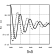
\includegraphics[width=1\linewidth]{Chapter_2/2} \\ а)}
	\end{minipage}
	\hfill
	\begin{minipage}[h]{0.5\linewidth}
		\center{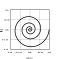
\includegraphics[width=0.9\linewidth]{Chapter_2/3} \\ б)}
	\end{minipage}
	\caption{(а,б). Затухающие колебания $(0<\gamma<\omega_0)$ при $\gamma/\omega_0=0,1$.}
	\label{fig2}
\end{figure}

Из формул \eqref{2.14}, \eqref{2.19} и рис.\ref{fig2} видно, что затухающие при условии $0<\gamma<\omega_0$ колебания напряжения и тока не являются периодическими функциями времени, однако эти величины дважды за время
\begin{equation}\label{2.23}
T_1=\dfrac{2\pi}{\omega_1}=\dfrac{T_0}{\sqrt{1-\gamma^2/\omega_0^2}}
\end{equation}
проходят через нуль. А так как согласно \eqref{2.2} нули функции $I(t)$ являются нулями функции $dU_C/dt,$ то величина $T_1$ представляет также время между двумя последовательными прохож\-дениями напряжения $U_C(t)$ через максимум (минимум). Очевидно, что экстремумы функции $I(t)$ чередуются с тем же периодом $T_1.$ Из этих результатов возникает (с понятной долей ус\-ловности) основание назвать  величину $T_1,$ определяемую формулами \eqref{2.23}, \textsf{периодом зату\-хающих колебаний.}

Взаимное расположение нулей и экстремумов $I(t)$ и $U_C(t)$ легко понять из энергетических соображений. Действительно, запасённая в контуре электромагнитная энергия заключена в электрическом поле конденсатора и магнитном поле катушки индуктивности, так что максимумы электрической энергии (экстремумы $U_C(t)$) достигаются в нулях $I(t),$ а максимумы магнитной энергии (экстремумы $I(t)$) достигаются в нулях $U_C(t).$

Отметим, что все экстремумы не находятся на серединах временных интервалов между соответствующими нулями, а сдвинуты влево на некоторую величину, возможность определить которую предоставляется читателю.

Из формулы \eqref{2.23} следует, что $T_1>T_0,$ то есть наличие потерь в контуре, обусловленных сопротивлением $R$ и представленных коэффициентом $\gamma,$ приводит к увеличению периода (уменьшению частоты) колебаний.

В качестве характеристик процесса затухания колебаний помимо коэффициента затухания $\gamma$ используют \textsf{время затухания}
\begin{equation}\label{2.24}
\tau=1/\gamma=2L/R,
\end{equation}
то есть время, за которое амплитуда колебаний убывает в $e$ раз, а также \textsf{логарифмический дек\-ремент}
\begin{equation}\label{2.25}
\Theta=\ln\dfrac{U_{Ck}}{U_{C(k+1)}}=\ln e^{\gamma T_1}=\gamma T_1,
\end{equation}
где $U_{Ck}$ и $U_{C(k+1)}$ \textbf{--} два последовательные максимальные отклонения рассматриваемой вели\-чины (в данном примере - напряжения на конденсаторе) в одну сторону от оси абсцисс. Из формул \eqref{2.24}, \eqref{2.25} следует связь между логарифмическим декрементом $\Theta$ и числом полных колебаний $N=\tau/T_1$ за время затухания $\tau:$
\begin{equation}\label{2.26}
\Theta=1/N.
\end{equation}
Таким образом, логарифмический декремент затухания $\Theta$ равен обратному числу $N$ периодов  $T_1,$ за которое амплитуда колебаний падает в $e$ раз.
 
На практике для определения $\Theta$ удобно использовать отношение максимальных отклонений, разделённых целым числом $n$ периодов $T_1$ (см. рис.\ref{fig2}). В этом случае формула для $\Theta$ принимает вид:
\begin{equation}\label{2.27}
\Theta=\dfrac{1}{n}\ln\dfrac{U_{Ck}}{U_{C(k+n)}}.
\end{equation}

Формулы \eqref{2.25} \textbf{--} \eqref{2.27} показывают, что максимумы (минимумы) функции $U_C(t)$ образуют убывающую геометрическую прогрессию со знаменателем
\begin{equation}\label{2.28}
U_{C(k+1)}/U_{Ck}=e^{-\Theta}.
\end{equation}
Такую же прогрессию образуют и экстремумы функции $I_C(t).$

Логарифмический декремент определяет \underline{шаг спи\-ра\-ли за\-ту\-ха\-ю\-ще\-го ко\-ле\-ба\-ния} на фазовой плоскости. Действительно, из формулы \eqref{2.28} следует, что
\begin{equation}\label{2.29}
U_{Ck}-U_{C(k+1)}=U_{Ck}\left(1-e^{-\Theta}\right).
\end{equation}
Рекомендуем читателю проверить, что кривые на рис.\ref{fig2} соответствуют $\gamma/\omega_0=0,1.$

С логарифмическим декрементом связана ещё одна характеристика колебательного контура \textbf{--} его \textsf{добротность}
{\large
\begin{equation}\label{2.30}
Q=\dfrac{\pi}{\Theta}=\dfrac{\pi}{\gamma T_1}=\pi N=\frac{1}{2}\sqrt{\omega_0^2/\gamma^2-1}
=\frac{1}{2}\sqrt{R_{\text{кр}}^2/R^2-1}=\sqrt{\rho^2/R^2-1/4}.
\end{equation}}

Как правило, о добротности говорят только тогда, когда добротность контура достаточно ве\-лика, то есть $Q\gg1.$ Такой добротностью обладают колебательные контуры со \textsf{слабым} за\-ту\-ха\-ни\-ем, представляющие большой практический интерес. Для них вместо неравенств $0<\gamma<\omega_0$ и \eqref{2.12} выполняются неравенства
\begin{equation}\label{2.31}
0<\gamma\ll\omega_0,
\end{equation}
или, в терминах параметров контура,
\begin{equation}\label{2.32}
0<R\ll2\sqrt{L/C}=2\rho=R_{\text{кр}}.
\end{equation}
Малость отношения $\gamma/\omega_0$ и связанных с ним характеристик контура:
\begin{equation}\label{2.33}
\gamma/\omega_0=R/2\rho=R/R_{\text{кр}}\ll1,
\end{equation}
\textbf{--} позволяет, пренебрегая вторыми и выше степенями в разложениях по этим малым величинам, значительно упростить уже полученные формулы, например, \eqref{2.15}, \eqref{2.17} \textbf{--}  \eqref{2.23}, \eqref{2.30}, и дальнейшие выкладки. Так, в этом приближении можно заменить $\omega_1$ и $T_1$ соответственно на $\omega_0$ и $T_0$, связать добротность $Q$ с другими характеристиками контура цепочкой равенств
\begin{equation}\label{2.34}
Q=\dfrac{\pi}{\gamma T_0}=\dfrac{\omega_0}{2\gamma}=\dfrac{\tau\omega_0}{2}=\dfrac{\omega_0L}{R}=\dfrac{1}{\omega_0CR}=\dfrac{1}{R}\sqrt{\dfrac{L}{C}}=\dfrac{\rho}{R},
\end{equation}
а напряжение на ёмкости и ток в контуре \eqref{2.22} представить в виде
\begin{equation}\label{2.35}
U_C(t)=U_{C0}e^{-\gamma t}[\cos\omega_0t+(\gamma/\omega_0)\sin\omega_0t],~~I(t)=-(U_{C0}/\rho)e^{-\gamma t}\sin\omega_0 t.
\end{equation}

В энергетическом смысле добротность $Q$ \underline{колебательной системы} (механической, электриче\-ской, оптической и т. д.) определяется как отношение запасённой в ней энергии $W$ к потере $\Delta W_1$ энергии за время $T/2\pi,$ за которое фаза колебания меняется на 1 радиан:
\begin{equation}\label{2.36}
Q=\dfrac{W}{\Delta W_1}=2\pi\dfrac{W}{\Delta W_T},
\end{equation}
где  $\Delta W_T$ \textbf{--} потеря энергии за период $T.$ При вычислении $\Delta W_T$ воспользуемся формулами \eqref{2.22} для представленных на рис.\ref{fig2} затухающих колебаний \underline{в рас\-сма\-три\-ва\-емом $LCR$-контуре}. Тот факт, что они получены для конкретных начальных условий: $U_C(0)=U_{C0},~~ I(0)=0,$ \textbf{--} не ска\-жется, естественно, на общности результата. Пусть в момент времени $t_0$ ток в контуре $I(t_0)=0,$ а напряжение на конденсаторе экстремально: $U_C(t_0)=\pm U_{C0}e^{-\gamma t_0}.$ Тогда ток равен нулю и в момент $t_0+T_1.$ В эти моменты времени в электрическом поле конденсатора сосредо\-точена вся энергия контура. При этом потеря энергии
\begin{equation}\label{2.37}
\Delta W_T=W(t_0)-W(t_0+T_1)=(1-e^{-2\gamma T_1})W(t_0),~~~
W(t_0)=e^{-2\gamma t_0}CU_{C0}^2/2.
\end{equation}
Формулы \eqref{2.37} справедливы и для моментов времени $t\ne t_0,$ однако, как уже говорилось выше при обсуждении нулей и экстремумов $I(t)$ и $U_C(t),$ электромагнитная энергия в этом случае распределяется между конденсатором и катушкой индуктивности, составляя в сумме величину $W(t).$

В случае \underline{слабого} затухания, когда выполняются неравенства \eqref{2.31}, формулу \eqref{2.37} можно упростить. В первом порядке по малому параметру $\gamma/\omega_0~~~\Delta W_T=4\pi(\gamma/\omega_0)W(t),$ так что $\Delta W_1=\Delta W_T/2\pi=(2\gamma/\omega_0)W(t).$ Для <<энергетической>> добротности \eqref{2.36} теперь приходим к формулам \eqref{2.34}, полученным в случае \underline{слабого} затухания из введённого в общем случае \underline{зату\-хающих} колебаний выражения для добротности \eqref{2.30}.

\textsf{Вариант 2:} $\gamma=\omega_0$ \textbf{--} \textsf{критический режим.} В этом случае параметры контура связаны соотно-шениями
\begin{equation}\label{2.38}
R=R_{\text{кр}}=2\sqrt{L/C}=2\rho,
\end{equation}
а уравнение \eqref{2.10} и его решение принимают вид: $\ddot{U}=0,~~U(t)=A_1+A_2t.$ Соответственно, напряжение на конденсаторе
\begin{equation}\label{2.39}
U_C(t)=(A_1+A_2t)e^{-\gamma t},
\end{equation}
где постоянные интегрирования $A_1$ и $A_2$ определяются начальными условиями задачи. Если, как и в \textsf{варианте 1,} приняты начальные условия: $U_C(0)=U_{C0,}~I(0)=0,$ \textbf{--} то для напряжения на конденсаторе и тока в контуре с учётом формул \eqref{2.9} и \eqref{2.2} получаем выражения:
\begin{equation}\label{2.40}
U_C(t)=U_{C0}(1+\gamma t)e^{-\gamma t},~~~I(t)=-(U_{C0}/\rho)\gamma te^{-\gamma t}.
\end{equation}
Отметим, что на практике этот режим, требующий строгого выполнения условия $\gamma=\omega_0,$ не может быть точно реализован и имеет значение как пограничный между режимом затухающих колебаний и рассматриваемого далее режимом апериодического затухания. 

\textsf{Вариант 3:} $\gamma>\omega_0$ \textbf{--} \textsf{апериодический режим.} В этом режиме $\omega_1^2=\omega_0^2-\gamma^2<0,$ так что для описания системы удобно перейти от тригонометрических функций к гиперболическим функ\-циям, введя вместо мнимой теперь величины $\omega_1$ действительную величину
\begin{equation}\label{2.41}
\alpha=\sqrt{\gamma^2-\omega_0^2}=\omega_0\sqrt{R^2/R_{\text{кр}}^2-1.}
\end{equation}
С помощью подстановки нетрудно убедиться, что общее решение уравнения \eqref{2.10} имеет при этом вид $U(t)=B_1e^{\alpha t}+B_2e^{-\alpha t},$ где постоянные величины $B_1$ и $B_2$ определяются начальными условиями. Соответственно, напряжение на конденсаторе
\begin{equation}\label{2.42}
U_C(t)=e^{-\gamma t}(B_1e^{\alpha t}+B_2e^{-\alpha t}).
\end{equation}
При начальных условиях $U_C(0)=U_{C0},~~I(0)=0$
{\large
\begin{equation}\label{2.43}
U_C(t)=U_{C0}e^{-\gamma t}[\ch \alpha t+(\gamma/\alpha)\sh \alpha t],~~~~
I(t)=-(U_{C0}/\rho)(\omega_0/\alpha)e^{-\gamma t}\sh \alpha t.
\end{equation}}

Как видно из \eqref{2.41}, апериодический режим реализуется, если параметры контура удовлетворя-ют условию
\begin{equation}\label{2.44}
R>R_{\text{кр}}=2\sqrt{L/C}=2\rho.
\end{equation}

Графики, соответствующие формулам \eqref{2.43}, а также фазовая траектория системы в аперио\-дическом режиме показаны в безразмерных переменных на рис.\ref{fig3}(a,\text{б}). На рис.\ref{fig2}a сплошная линия $u(x)=U_C(x)/U_{C0},$ где $x=\alpha t,$ соответствует напряжению на конденсаторе $U_C(t),$ а штриховая линия $j(x)=\rho I(x)/U_{C0}$ \textbf{--} току в контуре $I(t).$ На рис.\ref{fig3} \text{б} показана фазовая тра\-ектория этих колебаний на плоскости переменных $u(x),~j(x)$   при $\gamma/\omega_0=1,1~,$ представляющая собой короткий отрезок спирали.

\begin{figure}[h]
	\begin{minipage}[h]{0.49\linewidth}
		\centering
		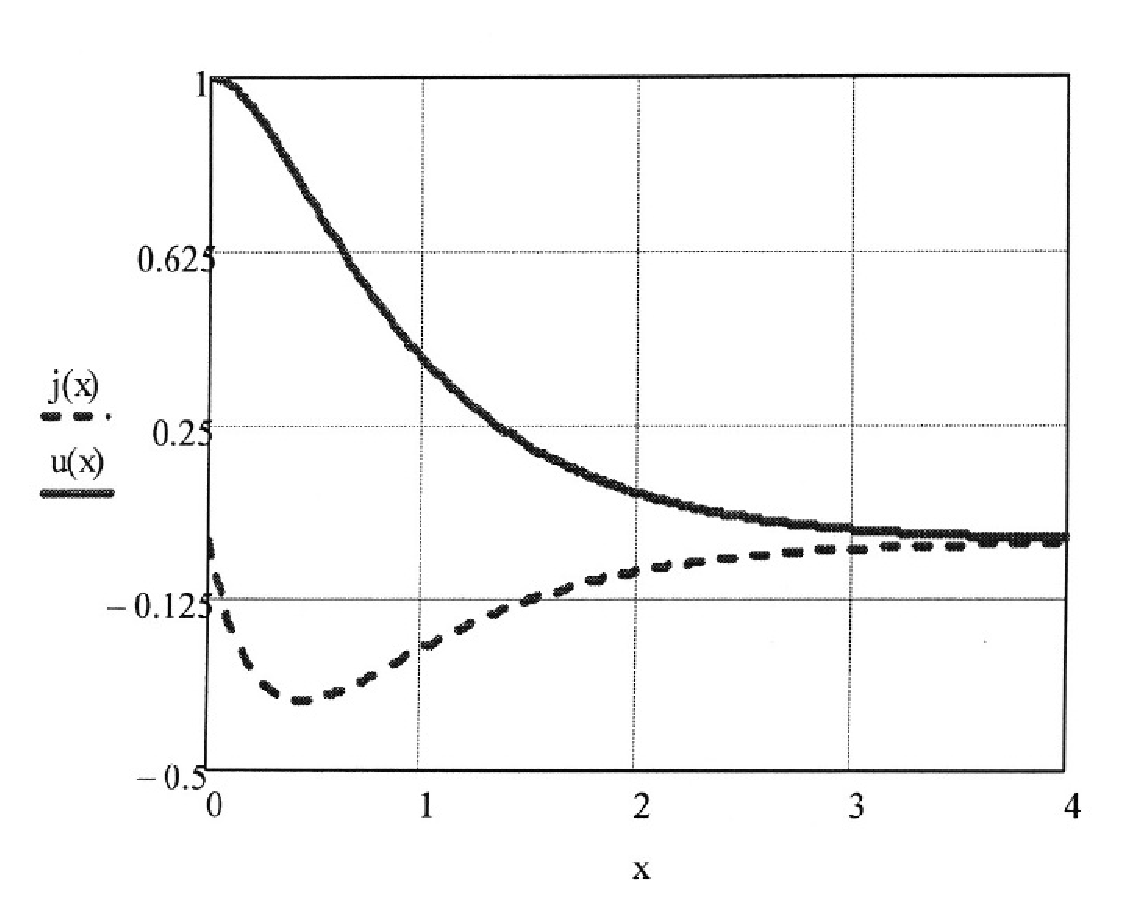
\includegraphics[width=1\linewidth]{Chapter_2/4}
		\caption{а}
	\end{minipage}
	\hfill
	\begin{minipage}[h]{0.49\linewidth}
		\centering
		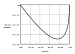
\includegraphics[width=0.9\linewidth]{Chapter_2/5}
		\caption{б}
	\end{minipage}
	\caption{(а,б).Апериодический режим $(\gamma>\omega_0)$ при $\gamma/\omega_0=1,1$.}
	\label{fig3}
\end{figure}

Как видно из рисунка, при выбранных начальных условиях в апериодическом режиме на-пряжение на емкости убывает монотонно, а ток перед монотонным убыванием совершает коле\-бание, не меняя направления. Можно показать, что в этом режиме при любых начальных усло\-виях система стремится к равновесному состоянию $U_C=0,~~I=0.$ При этом возможно не более одного прохождения через экстремальное  состояние, как на рис.\ref{fig3}, и не более одного \textbf{--} через равновесное.

\begin{center}
	\textbf{2. Вынужденные колебания. Метод комплексных амплитуд. Векторные диаграммы}
\end{center}

Рассмотрим процессы, протекающие в контуре, подключённом к источнику внешней ЭДС, изменяющейся по гармоническому закону:  $\varepsilon=\varepsilon_0\cos(\omega t+\varphi_0).$ Соответствующая схема пред\-ставлена на рис.\ref{fig4}.

\begin{figure}[h!]
	\centering
	\includegraphics[width=0.25\linewidth]{Chapter_2/6}
	\caption{Последовательный контур с внешней гармонической ЭДС}
	\label{fig4}
\end{figure}

Потерями в конденсаторе и в катушке индуктивности в аналитических выкладках будем пренебрегать, как и в п.1 при рассмотрении свободных колебаний. Потери в катушке индуктивности учтём при рассмотрении векторных диаграмм.

%\begin{center}
%		\begin{figure}[h!]
%			\centering\includegraphics[width=0.25\linewidth]{6}
%			\caption{Последовательный контур\\
%				 с внешней гармонической ЭДС\\}
%			\label{fig4}
%		\end{figure}
%\end{center}

Для напряжения на конденсаторе $U_C(t)$ вместо \eqref{2.8} получим теперь уравнение
\begin{equation}\label{2.45}
\ddot{U}_C+2\gamma \dot{U}_C+\omega_0^2U_C=\omega_0^2\varepsilon_0\cos(\omega t+ \varphi_0).
\end{equation}
Решение \underline{линейного} дифференциального уравнения \eqref{2.45} с правой частью состоит из общего решения однородного уравнения и какого-либо частного решения данного уравнения с правой частью. Как показано в предыдущем разделе, собственные свободные колебания контура (об\-щее решение) при любых начальных условиях экспоненциально затухают. Со временем их ам\-плитуда становится пренебрежимо малой, и в системе остаются только вынужденные ко\-ле\-ба\-ния (частное решение), обусловленные действием внешней ЭДС. Для нахождения этого частного решения воспользуемся \underline{методом комплексных амплитуд.} Данный метод основан на следующем ут\-вер\-жде\-нии: \emph{пусть некоторая комплексная функция является решением линейного дифференциального уравнения с вещественными коэффициентами и комплексной правой ча\-стью; тогда вещественная часть этой функции является решением того же уравнения, в пра\-вой части которого стоит вещественная часть прежнего выражения, а мнимая часть – ре\-шением уравнения с мнимой правой частью.}

Исходя из сказанного, перейдём к комплексному представлению колебаний и запишем урав\-нение \eqref{2.45} в комплексной форме, отмечая комплексные величины ''стрелкой'':
$$
U_C=Re\vec U_C,~~~~\vec U_C=Re\vec U_C+i\text{Im}\vec U_C,~~~~\varepsilon=Re\vec \varepsilon,~~~~\vec \varepsilon=\vec \varepsilon_0e^{i\omega t}=\varepsilon_0e^{i(\omega t+\varphi_0)},
$$
\begin{equation}\label{2.46}
\dfrac{d^2\vec U_C}{dt^2}+2\gamma\dfrac{d\vec U_C}{dt}+\omega_0^2\vec U_C=\omega_0^2\varepsilon_0e^{i(\omega t+\varphi_0)}.
\end{equation}
Комплексная величина $\vec \varepsilon_0=\varepsilon_0e^{i\varphi_0},$ стоящая перед $e^{i\omega t},$ называется \textsf{комплексной амплитудой} (в данном случае это относится к внешней ЭДС). Решив уравнение \eqref{2.46}, мы получим комплекс\-ное выражение для напряжения на конденсаторе. \underline{Вещественная часть} этого решения является, согласно приведённому выше утверждению, решением исходного уравнения \eqref{2.45}.

Будем искать решение уравнения \eqref{2.46} в виде:
\begin{equation}\label{2.47}
\vec U_C(t)=\vec U_{C0}e^{i\omega t},
\end{equation}
где $\vec U_{C0}$ \textbf{--} комплексная амплитуда напряжения на конденсаторе, не зависящая от времени. Подставляя \eqref{2.47} в \eqref{2.46} находим $\vec U_{C0},$ и далее, используя формулы \eqref{2.2}, \eqref{2.1}, \eqref{2.3}, \textsf{--} комплексные амплитуды тока в контуре и напряжений на сопротивлении и индуктивности:

$$%\begin{equation}
\vec U_{C0}=(1/i\omega CZ)\varepsilon_0 e^{i\varphi_0},~~~Z=R+i(\omega L-1/\omega C) \eqno(2.48a)
$$%\end{equation}
{\large
$$%\begin{equation}\label{2.48b}
\vec I_0=i\omega C\vec U_{C0}=(1/Z)\varepsilon_0 e^{i\varphi_0},~~\vec U_{R0}=R\vec I_0=(R/Z)\varepsilon_0 e^{i\varphi_0},~~
\vec U_{L0}=i\omega L\vec I_0=(i\omega L/Z)\varepsilon_0e^{i\varphi_0} \eqno(2.48\text{б})
$$%\end{equation}}

Комплексная величина $Z$ в формулах (2.48), называется \textsf{комплексным сопротивлением,} или \textsf{импедансом,} последовательного контура и пишется обычно без ``стрелки``. Аналогичные обо\-значения можно ввести и для отдельных элементов контура. Таким образом,
{\large
\setcounter{equation}{48}
\begin{equation}\label{2.49}
	Z\equiv Re Z+i\text{Im}Z=R+i(\omega L-1/\omega C),~~~Z_R=R,~~~Z_L=i\omega L,~~~
	Z_C=-i/\omega C.
\end{equation}}

В этих обозначениях уравнения (2.48) принимают вид:
\begin{equation}\label{2.50}
	\vec I_0=\vec \varepsilon_0/Z,~~~~\vec U_{R0}=Z_R\vec I_0,~~~~\vec U_{C0}=Z_C\vec I_0,~~~~\vec U_{L0}=Z_L\vec I_0.
\end{equation}
Выражения \eqref{2.50} представляют обобщение закона Ома для переменных токов. Роль сопротив\-лений в них играют импеданс контура $Z$ в первом случае и импедансы его отдельных элемен\-тов \textsf{--} в остальных случаях.

Важно отметить, что импеданс контура $Z$ не зависит от начальных условий, не содержит ве\-личин ни токов, ни напряжений, а определяется свойствами всех элементов, соединённых в контур, и частотой синусоидальной ЭДС, к которой он подключён. Таким образом, \underline{импеданс $Z$ является характеристикой ко\-ле\-ба\-тель\-но\-го кон\-ту\-ра на заданной частоте.}

Выражение для $Z$ содержит действительную часть $ReZ=R,$ называемую обычно \textsf{активным сопротивлением} контура, и мнимую часть $\text{Im}Z=\omega L-1/\omega C,$ носящую название \textsf{реактивного сопротивления.} \underline{Правила сложения импедансов отдельных элементов схе\-мы при пос\-ле\-до-} \underline{ва\-тель\-ном и параллельном включении – те же, что и для обыкновенных сопротивлений.}

Импедансы реальных конденсаторов и катушек самоиндукции содержат кроме мнимой час\-ти, также и действительную часть. Действительная часть импеданса определяется необратимы\-ми потерями энергии, которые могут быть связаны как с омическим сопротивлением проводников, так и с другими причинами: с утечками и диэлектрическими потерями в конденсаторах, с токами перемагничивания и токами Фуко в магнитных сердечниках катушек самоиндукции. Потери в конденсаторах и в катушках самоиндукции зависят как от частоты, так и от амплитуды проходящего через них тока. Поэтому, приводя величины эквивалентного сопротивления потерь в этих элементах, следует указывать частоту и амплитуду тока, при которых данные величины были измерены.

Импедансы контура и его отдельных элементов – комплексные числа – могут быть представлены в показательной форме. Для импеданса рассматриваемого последовательного контура при этом находим:
$$%\begin{equation}\label{2.51}
Z=Z_0e^{i\psi_I},~~~~Z_0=\sqrt{R^2+(\omega L-1/\omega C)^2}=R/\cos\psi_I, \eqno(2.51a)
$$%\end{equation}
$$%\begin{equation}\label{2.51b}
\tg\psi_I=\text{Im}Z/ReZ=(\omega L-1/\omega C)/R,~~\psi_I=\arctg[(\omega L-1/\omega C)/R].\eqno(2.51\text{б})
$$%\end{equation}
Интересующие нас ток в контуре и напряжения на отдельных его элементах теперь могут быть получены по формулам (2.48) \textbf{--} \eqref{2.50}. Например, действительная часть тока в контуре 
\setcounter{equation}{51}
\begin{equation}\label{2.52}
	I(t)=(\varepsilon_0/Z_0)\cos(\omega t+\varphi_0-\psi_I)=(\varepsilon_0\cos\psi_I/R)/cos(\omega t+\varphi_0-\psi_I).
\end{equation}

Как видно из этой формулы, угол $\psi_I,$ определяемый отношением мнимой и действительной частей импеданса, представляет собой сдвиг фаз между напряжением на последовательном контуре и током в нём, причём \underline{положительные зна\-че\-ния угла} $\psi_I$ \underline{соответствуют отставанию} \underline{фазы тока}, \underline{а отрицательные – опе\-ре\-же\-нию}. В общем случае, когда к источнику пос\-ле\-до\-ва\-тель\-но подключены резистор, конденсатор и катушка самоиндукции, сдвиг фазы тока $\psi_I$ лежит в пределах $-\pi/2<\psi_I<\pi/2.$ Из формулы \eqref{2.52} также видно, что от угла $\psi_I$ зависит амплитуда тока, а следовательно, и средняя мощность активных потерь в контуре
\begin{equation}\label{2.53}
	P=\langle I^2R\rangle_T=\varepsilon_0^2\cos^2\psi_I/2R,
\end{equation}
где угловые скобки с индексом <<$T$>> означают усреднение по периоду колебаний.
Решения, полученные методом комплексных амплитуд, допускают простую геометрическую интерпретацию. Комплексное число, например, напряжение $\vec \varepsilon=\vec \varepsilon_0e^{i\omega t}=\varepsilon_0e^{i(\omega t+\varphi_0)},$ представляется в комплексной плоскости вектором, длина которого равна $\varepsilon_0$ \textbf{--} амплитуде напряжения $\varepsilon(t),$ а угол, составляемый этим вектором с вещественной осью, равен $\omega t+\varphi_0$ \textbf{--} фазе напряжения $\varepsilon(t).$ Вектор $\vec \varepsilon$ вращается с угловой скоростью $\omega$ против часовой стрелки. Удобно перейти к системе координат, которая сама вращается с угловой скоростью $\omega.$ В этой системе вектор $\vec \varepsilon$ будет представлен покоящимся вектором $\vec \varepsilon_0=\varepsilon_0e^{i\varphi_0},$ а векторы $\vec I_0, \vec U_{C0}, \vec U_{R0}$ и $\vec U_{L0}$ будут неподвижны, но окажутся сдвинутыми по углу относительно вектора $\vec \varepsilon_0.$ Вектор $\vec I_0,$ как показано выше, сдвинут от вектора $\vec \varepsilon_0$ на угол $\psi_I,$ определяемый формулами (2.51).

Положения остальных векторов легко определить по формулам (2.48). Так, наличие множи\-теля $i=exp(i\pi/2)$ в первом равенстве в (2.48 \text{б}) означает, что вектор $\vec I_0$ опережает по углу на $\pi/2$ вектор $\vec U_{C0},$ то есть ток опережает напряжение на конденсаторе по фазе на $\pi/2.$ Анало\-гично, множитель $i=exp(i\pi/2)$ в третьем равенстве в (2.48 \text{б}) показывает, что напряжение на индуктивности $\vec U_{L0}$ опережает по фазе ток $\vec I_0$ на угол $\pi/2.$ Наконец, из второго равенства в (2.48 \text{б}) видно, что вектор $\vec U_{R0}$ совпадает по направлению с вектором $\vec I_0,$ и, значит, напряжение на сопротивлении совпадает по фазе с током $\vec I_0$. Построенные таким образом диаграммы назы\-ваются \textsf{векторными.}

В качестве примера построим векторную диаграмму тока и напряжений для последователь\-ного контура. Рассмотрим схему, изображённую на рис.\ref{fig5}. К источнику переменного напряжения $\varepsilon=\varepsilon_0\cos\omega t$ последовательно подключены резистор $R,$ катушка индуктивности $L,$ действительная часть импеданса которой равна $r_L$, и ёмкость $C.$ Активное сопротивление $r_L$ катушки индуктивности, которое с целью упрощения не учитывалось выше при аналитическом решении задачи и будет учтено в описаниях соответствующих лабораторных работ, легко может быть найдено в представленной на рисунке <<схеме четырёх вольтметров>> с использованием векторной диаграммы. Вольтметры измеряют напряжения на элементах цепи, амперметр измеряет ток. Поскольку во всех элементах цепи ток $I$ одинаков, удобно положить его фазу равной нулю и отсчитывать от неё фазы напряжений на всех элементах цепи, определив затем фазу   между напряжением на контуре и током.

\begin{figure}[h]
	\begin{minipage}[h]{0.37\linewidth}
		\centering
		\includegraphics[width=1\linewidth]{Chapter_2/7}
		\caption{а}
	\end{minipage}
	\hfill
	\begin{minipage}[h]{0.49\linewidth}
		\centering
		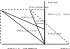
\includegraphics[width=1\linewidth]{Chapter_2/8}
		\caption{б}
	\end{minipage}
	\caption{(а,б).Схема измерения (а) и векторная  диаграмма (б) для последовательного контура}
	\label{fig5}
\end{figure}

Отложим вектор $\vec I$вдоль оси ординат (рис.\ref{fig5}\text{б}). Напряжение на резисторе совпадает по фа\-зе с током, поэтому вектор $\vec U_R$ также будет направлен вдоль оси ординат. Напряжение на кон\-денсаторе (без потерь) отстаёт по фазе от тока на угол $\pi/2,$ поэтому вектор $\vec U_C$ направлен пер\-пендикулярно вектору $\vec I$ в сторону положительных значений абсцисс. Векторное равенство напряжений $\vec U_{L+R}=\vec U_L+\vec U_R$ позволяет построить треугольник по трём сторонам. Для этого сделаем две насечки: первую – радиусом, равным модулю вектора $\vec U_{L+R},$ из начала этого век\-тора (начала координат), вторую – радиусом, равным модулю вектора $\vec U_L,$ из конца вектора $\vec U_R.$ Точка пересечения насечек определяет положение векторов $\vec U_{L+R}$ и $\vec U_L$ на диаграмме. Сложив векторы $\vec U_{L+R}$ и $\vec U_C,$ получим вектор $\vec\varepsilon$ входного напряжения на контуре. Угол $\psi_I$ показывает, каков сдвиг фаз между током и напряжением в цепи. Разложим теперь вектор $\vec U_L$ по осям координат. Проекция $\vec U_L$ на ось ординат позволяет определить $\vec U_{L,\text{акт}}$ – напряжение на активной части импеданса катушки, а проекция на ось абсцисс даёт реактивную часть $\vec U_{L,\text{реакт}}.$ Поделив эти напряжения на ток $I,$ найдём действительную $r_L$ и мнимую $\omega L$ части импеданса катушки.

\begin{center}
\textbf{3. Вынужденные колебания. Резонанс}
\end{center}
\textsf{3.1. Резонанс напряжений в последовательном контуре.} В предыдущем разделе были полу\-чены выражения (2.48), описывающие в комплексной форме вынужденные колебания в после\-довательном контуре под действием внешней гармонической ЭДС. Там же указывалось, что эти колебания устанавливаются в системе после затухания собственных свободных колебаний контура. Процесс установления вынужденных колебаний будет рассмотрен отдельно в п.4 данного раздела. Для исследования вынужденных колебаний и резонанса запишем \underline{вещественные части} решений (2.48), использовав формулы \eqref{2.7} и \eqref{2.12} для собственной частоты $\omega_0$ и волнового сопротивления $\rho,$ а также положив для сокращения записи раной нулю начальную фазу: $\varphi_0=0$. В результате приходим к уравнениям:
$$%\begin{equation}\label{2.54}
I(t)=U_R(t)/R=I_{\omega}\cos(\omega t-\psi_I),~~~~~I_{\omega}=\varepsilon_0/Z_0,\eqno(2.54a)
$$%\end{equation}
$$%\begin{equation}\label{2.54b}
Z_0=R\sqrt{1+(\rho/R)^2(\omega/\omega_0-\omega_0/\omega)^2,}~~~~~\psi_I=\arctg[(\rho/R)(\omega/\omega_0-\omega_0/\omega)],\eqno(2.54\text{б})
$$%\end{equation}
$$%\begin{equation}\label{2.54c}
U_C(t)=U_{C\omega}\cos(\omega t-\psi_C),~~~~U_{C\omega}=\varepsilon_0\dfrac{\rho}{Z_0}\dfrac{\omega_0}{\omega},~~~\psi_C=\psi_I+\pi/2,\eqno(2.54\text{в})
$$%\end{equation}
$$%\begin{equation}\label{2.54d}
U_L(t)=U_{L\omega}\cos(\omega t-\psi_L),~~~~U_{L\omega}=\varepsilon_0\dfrac{\rho}{Z_0}\dfrac{\omega}{\omega_0},~~~\psi_L=\psi_I-\pi/2.\eqno(2.54\text{г})
$$%\end{equation}

Отметим, что аналитическое выражение из (2.54 \text{б}) для фазового сдвига $\psi_I$ между внешней ЭДС и током в контуре легко упрощается в наиболее интересной области, лежащей вблизи соб\-ственной частоты контура $\omega_0,$ а фазовые сдвиги $\psi_C$ и $\psi_L$ связаны с $\psi_I$ простыми соотноше\-ниями из (2.54 \text{в}) и (2.54 \text{г}). Напомним также, что согласно формуле \eqref{2.53} от угла $\psi_I$ зависит средняя мощность активных потерь в контуре.

Следует, однако, подчеркнуть, что в выражениях (2.54) не учтены <<паразитные>> индуктивности и емкости реактивных элементов схемы, а также возможные потери энергии в них. Необходимые уточнения будут сделаны в описаниях соответствующих лабораторных работ.

Важно также отметить, что <<по умолчанию>> в нашем рассмотрении пренебрегалось внут\-ренним сопротивлением источника ЭДС, то есть считалось, что он является \textsf{генератором на\-пряжения,} который по определению обладает \underline{нулевым внутренним со\-про\-тив\-ле\-ни-} \underline{ем.} В этом случае амплитуда $\varepsilon_0$ не зависит от меняющегося с частотой сопротивления нагрузки – последовательного колебательного контура.

Анализ формул (2.54) позволяет сделать следующие выводы.

1) При заданных параметрах $\varepsilon_0$ и $\omega$ внешнего источника напряжения зависимости амплитуд и фаз тока и напряжений в системе от частоты – \textsf{амплитудные} и \textsf{фазовые характеристики сис\-темы} – определяются двумя безразмерными величинами: $\rho/R$ и $\omega/omega_0.$ Как следует из формул \eqref{2.33}, \eqref{2.34}, для контура со \underline{слабым} затуханием, для которого добротность $Q\gg1,$ отношение $\rho/R=Q,$ как уже отмечалось выше.

2) Поведение системы носит резонансный характер: при $\omega=\omega_0,$ когда мнимая часть импеданса контура $\text{Im}Z=0$ и, соответственно,
\setcounter{equation}{54}
\begin{equation}\label{2.55}
	\omega_0L=1/\omega_0C=\rho,
\end{equation}
подкоренные выражения в формулах для амплитуд принимают минимальное значение, равное единице, амплитуды тока и напряжения на сопротивлении достигают максимальных значений
\begin{equation}\label{2.56}
	I_{\omega_0}=\varepsilon_0/R,~~~~~~~U_{R\omega_0}=RI_{\omega_0}=\varepsilon_0
\end{equation}
и совпадают по фазе с ЭДС, поскольку $\psi_0.$ Таким образом, последовательный контур на собственной частоте $\omega_0$ представляет для внешней ЭДС чисто активную нагрузку, на которой согласно \eqref{2.53} выделяется мощность $P_{\text{max}}=\varepsilon_0^2/2R.$

3) Наиболее ярко резонансный характер вынужденных колебаний в \underline{пос\-ле\-до\-ва-} \underline{тель\-ном} контуре проявляется в напряжениях на конденсаторе и индуктивности, которые при $\omega=\omega_0$ в $\rho/R$ раз превышают напряжение $\varepsilon_0$ по амплитуде и сдвинуты по фазе от него на $\mp\pi/2$ соответственно и, значит, находятся в противофазе друг с другом. Последние утверждения, правда, относятся к идеальному случаю отсутствия потерь в этих элементах. При добротности $Q=\rho/R\gg1$ ам\-плитуды напряжений $U_C(t)$ и $U_L(t)$ значительно превышают амплитуду $\varepsilon_0$ напряжения на контуре. По этой причине резонанс в последовательном контуре называется \textsf{резонансом напря\-жений.}

4) Наличие множителей   в формулах (2.54 \text{в}), (2.54 \text{г}) приводит к тому, что \underline{максимумы} напряжений на конденсаторе и индуктивности равны друг другу, превышают $(\rho/R)\varepsilon_0$ и сдви\-нуты в разные стороны от собственной частоты контура $\omega_0,$ на которой достигаются максиму\-мы тока и напряжения на сопротивлении $R:$
{\large
\begin{equation}\label{2.57}
	U_{C\omega_\text{m}}=U_{L\omega_\text{m}}=(\rho/R)\varepsilon_0[1-1/4(\rho/R)^2]^{-1/2},~~~\omega_{\text{m},C,L}=\omega_0[1-1/2(\rho/R)^2]^{\pm1/2}.
\end{equation}}
Рекомендуем читателям убедиться в этом самостоятельно.

Частоты, на которых достигаются \underline{максимальные} значения величин, характеризующих выну\-жденные колебания в различных колебательных системах, принято называть \textsf{резонансными.} Таким образом, в последовательном колебательном контуре резонансной частотой для тока $I$ и напряжения на сопротивлении $U_R$ является собственная частота контура $\omega_0,$ для напряжения на конденсаторе $U_C$ – частота $\omega_{\text{m}C}=\omega_0[1-1/2(\rho/R)^2]^{+1/2},$ для напряжения на индуктивности $U_L$ – частота $\omega_{\text{m}L}=\omega_0[1-1/2(\rho/R)^2]^{-1/2},$ причём $\omega_{\text{m}C}\cdot\omega_{\text{m}L}=\omega_0^2.$
	
На рис.\ref{fig6} приведены \underline{в безразмерном виде} кривые зависимостей от $x\equiv\omega/\omega_0$ амплитуды тока $j(x)\equiv RI_\omega/\varepsilon_0$ (рис.\ref{fig6} a) и амплитуды напряжения на конденсаторе $u(x)\equiv U_{C\omega}/\varepsilon_0$  (рис.\ref{fig6} \text{б}) при трёх значениях отношения $\rho/R,$ равных 2,~5 и 10.

\begin{figure}[h]
	\begin{center}
		\begin{minipage}[h]{0.45\linewidth}
			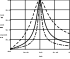
\includegraphics[width=1\linewidth]{Chapter_2/9}
			\caption{а} 
			\label{fig6} 
		\end{minipage}
		\hfill
		\setcounter{figure}{5}
		\begin{minipage}[h]{0.45\linewidth}
			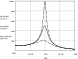
\includegraphics[width=1\linewidth]{Chapter_2/10}
			\caption{б}
			\label{fig9}
		\end{minipage}
	\end{center}
\end{figure}

Эти кривые называются \textsf{амплитудными резонансными кривыми} колебательного контура. Важ\-ными характеристиками резонансных кривых являются \underline{мак\-си\-маль\-ное значение ам\-пли-} \underline{ту\-ды} соответствующей величины и \underline{ширина ре\-зо\-нанс\-ной кривой}, при которой амплитуда этой величины уменьшается в $\sqrt{2}$ раз по сравнению со своим максимальным значением и в 2 раза уменьшается мощность сигнала. В частности, по этим характеристикам можно определить добротность колебательного контура. Например, эту величину можно определить по отношению максимального значения напряжения на конденсаторе $U_C$ к его статическому значению при $\omega=0,$ равному $\varepsilon_0,$ что следует из формул (2.54) и видно из рис.\ref{fig6} \text{б}.

Как уже отмечалось, о резонансе, как правило, говорят, если добротность $Q$ колебательного контура достаточно велика и, следовательно, выполняются соотношения \eqref{2.34}. Наибольший практический интерес представляет случай, когда отклонение $\Delta\omega\equiv\omega-\omega_0$ частоты внешней ЭДС от собственной частоты контура с добротностью $Q=\rho/R\gg1$ удовлетворяет сильному неравенству
\begin{equation}\label{2.58}
	|\Delta\omega|\ll\omega_0.
\end{equation}
При этом в первом порядке малости по \textsf{относительной расстройке частоты} $\Delta\omega/\omega_0$
\begin{equation}\label{2.59}
	\dfrac{\omega}{\omega_0}-\dfrac{\omega_0}{\omega}=\dfrac{2\Delta\omega}{\omega_0},
\end{equation}
что позволяет упростить выражения (2.54 \text{б}) и представить их в виде:
$$%\begin{equation}\label{2.60}
Z_0=R\sqrt{1+(\tau\Delta\omega)^2},~~~~~\psi_I=\arctg(\tau\Delta\omega),\eqno(2.60a)
$$%\end{equation}
где по определению \eqref{2.24} $\tau=1/\gamma$ – время затухания колебательного контура. Соответственно упрощаются и выражения для амплитуд $I_{\omega},~U_{C\omega} и U_{L\omega}$ в остальных формулах (2.54), в кото\-рые входит импеданс контура $Z_0$:
$$%\begin{equation}\label{2.60b}
I_{\omega}=\dfrac{\varepsilon_0}{R\sqrt{1+(\tau\Delta\omega)^2}},~~~~~U_{C\omega}=\dfrac{Q\varepsilon_0(\omega_0/\omega)}{\sqrt{1+(\tau\Delta\omega)^2}},~~~~~U_{L\omega}=\dfrac{Q\varepsilon_0(\omega/\omega_0)}{\sqrt{1+(\tau\Delta\omega)^2}}.\eqno(2.60\text{б})
$$%\end{equation}
На собственной частоте, когда $\omega=\omega_0,~\Delta\omega,$ выражения для амплитуд тока и напряжений на ёмкости и индуктивности, фазовых сдвигов и их производных по частоте $\omega$ принимают вид:
$$%\begin{equation}\label{2.61}
I_{\omega}(\omega_0)=U_{R\omega}(\omega_0)/R=\varepsilon_0/R,~~~~~\psi_I(\omega_0)=0,\eqno(2.61a)
$$%\end{equation}
$$%\begin{equation}\label{2.61b}
U_{C\omega}(\omega_0)=U_{L\omega}(\omega_0)=Q\varepsilon_0,~~~~\psi_C(\omega_0)=-\psi_L(\omega_0)=-\pi/2,\eqno(2.61\text{б})
$$%\end{equation}
$$%\begin{equation}\label{2.61c}
\psi'_I(\omega_0)=\psi'_L(\omega_0)=\psi'_C(\omega_0)=\tau.\eqno(2.61\text{в})
$$%\end{equation}
Напомним, что максимальные (резонансные) значения напряжений на ёмкости и индуктивности не строго равны $Q\varepsilon_0$ и достигаются не строго на частоте $\omega_0.$ Соответствующие относительные поправки, как это следует из формул \eqref{2.57}, в рассматриваемом случае высокой добротности, когда $Q\approx\rho/R\gg1,$ составляют доли малой величины $Q^{-2}$ и не учтены в (2.61).

При отклонении $\Delta\omega=\omega-\omega_0=\Delta\omega{\gamma}$ таком, что выполняется условие
\setcounter{equation}{61}
\begin{equation}\label{2.62}
\Delta\omega_{\gamma}=\pm\gamma,~~\text{или}~~\tau\Delta\omega{\gamma}=\pm1,
\end{equation}
амплитуда тока $I_{\omega},$ как видно из формул (2.60), уменьшается в $\sqrt{2}$ раз относительно своей мак\-симальной (резонансной) величины, а фаза $\psi_I$ изменяется на угол $\pm\pi/4.$ Аналогичные измене\-ния происходят с амплитудами $U_{C\omega},~U_{L\omega}$ и фазами $\psi_C,~\psi_L$   напряжений на ёмкости и индук\-тивности: амплитуды уменьшаются в $\sqrt{2}$ раз, а фазы меняются на угол $\pm\pi/4$ по отношению к своим резонансным значениям.

Величина $\delta\omega\equiv2|\Delta\omega_{\gamma}|=2\gamma=2/\tau$ представляет собой важную характеристику ко\-ле\-ба\-тель\-ного контура – \textsf{ширину резонансной кривой} $U_C(\omega),$ по которой с учётом соотношений $Q=\omega_0/2\gamma=\tau\omega_0/2$ из \eqref{2.34}, зная резонансную частоту $\omega_0$, можно найти добротность контура
\begin{equation}\label{2.63}
Q=\dfrac{\omega_0}{\delta\omega}.
\end{equation}

Ширину резонансной кривой и добротность можно определить и по фазово-частотным ха\-рактеристикам контура. Например, тангенс угла наклона кривой $\psi_C(\omega)$ в точке резонанса со\-гласно (2.61\text{в}) равен времени затухания $\tau=2/\delta\omega,$ а расстояние по оси $\omega$ между точками, в которых фаза $\psi_C$ меняется от $\pi/4$ до $3\pi/4,$ равно $2/\tau=\delta\omega.$

Следует отметить, что в соотношении $\tau\cdot\delta\omega\sim1,$ которому подчиняется произведение вре\-мени затухания и ширины резонансной кривой колебательного контура, проявляется фундаментальное \emph{соотношение неопределённости,} связывающее, в частности, <<время жизни>> $\tau$ квантового осциллятора с шириной спектральной линии $\delta\omega$ его излучения (см., например, [1], с.390).

\textsf{3.2. Резонанс токов в параллельном контуре.} Рассмотрим теперь вынужденные колебания в параллельном контуре, одна из ветвей которого содержит индуктивность $L$ и сопротивление $R,$ а другая – ёмкость $C$ (рис.\ref{fig7}).
\begin{center}
	\begin{figure}[h!]
		\centering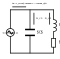
\includegraphics[width=0.25\linewidth]{Chapter_2/11}
		\caption{Параллельный контур с внешней гармонической ЭДС}
		\label{fig7}
	\end{figure}
\end{center}

Контур подключён к источнику ЭДС, задающему во внешней цепи ток, изменяющийся по гармоническому закону: $I=I_0\cos(\omega t+\varphi_0).$ Таким образом, мы предполагаем, что внутреннее сопротивлением источника столь велико, что он является \textsf{генератором тока,} который по оп\-ределению обладает \underline{бесконечно большим внутренним} \underline{сопротивлением.} Потерями в катушке индуктивности и конденсаторе будем пренебрегать, как это делалось и при рассмотрении резо\-нанса напряжений в последовательном контуре. Необходимые уточнения будут сделаны в опи\-саниях соответствующих лабораторных работ.

Воспользовавшись формулами \eqref{2.49}, правилами сложения сопротивлений и правилами Кирхгофа, для комплексных амплитуд токов в ёмкостной $\vec I_C$ и индуктивной $\vec I_L$ ветвях контура, а также для напряжения $\vec U$ на контуре, совпадающем в нашем приближении с напряжением на конденсаторе, при начальной фазе $\varphi_0=0$ тока $\vec I=I_0e^{i\varphi_0}$ во внешней цепи получаем выражения:
$$%\begin{equation}\label{2.64}
\vec I_C=\vec I\dfrac{Z_{LR}}{Z_C+Z_{LR}}=i\dfrac{\rho\omega}{R\omega_0}I_0\dfrac{1-iR\omega_0/\rho\omega}{1+i(\rho/R)(\omega/\omega_0-\omega_0/\omega)},\eqno(2.64a)
$$%\end{equation}
$$%\begin{equation}\label{2.64b}
\vec I_L=\vec I\dfrac{Z_C}{Z_C+Z_{LR}}=-i\dfrac{\rho\omega_0}{R\omega}I_0\dfrac{1}{1+i(\rho/R)(\omega/\omega_0-\omega_0/\omega)},\eqno(2.64\text{б})
$$%\end{equation}
$$%\begin{equation}\label{2.64c}
\vec U=\vec IZ=\vec I\dfrac{Z_CZ_{LR}}{Z_C+Z_{LR}}=\dfrac{\rho^2}{R}I_0\dfrac{1-iR\omega_0/\rho\omega}{1+i(\rho/R)(\omega/\omega_0-\omega_0/\omega)},\eqno(2.64\text{в})
$$%\end{equation}
где $Z_C$ и $Z_{LR}$ – импедансы емкостной и индуктивной ветвей параллельного контура соответственно.

Ограничимся рассмотрением наиболее интересного случая контура с высокой добротно\-стью вблизи резонансной частоты, когда $Q=\rho/R\gg1,$ выполняется условие \eqref{2.58} и примени\-мо разложение \eqref{2.59}. При этом \underline{вещественные части ком\-плекс\-ных амплитуд} (2.64) можно представить в виде
$$%\begin{equation}\label{2.65}
I_C(t)=QI_0\dfrac{\omega}{\omega_0}\dfrac{\cos(\omega t-\psi_C)}{R\sqrt{1+(\tau\Delta\omega)^2}},~~~~~~~~\psi_C=\arctg(\tau\Delta\omega)-\dfrac{\pi}{2}+Q^{-1},\eqno(2.65\text{а})
$$%\end{equation}
$$%\begin{equation}\label{2.65b}
I_L(t)=QI_0\dfrac{\omega_0}{\omega}\dfrac{\cos(\omega t-\psi_L)}{\sqrt{1+(\tau\Delta\omega)^2}},~~~~~~~~\psi_L=\arctg(\tau\Delta\omega)+\dfrac{\pi}{2},\eqno(2.65\text{б})
$$%\end{equation}
$$%\begin{equation}\label{2.65c}
U(t)=Q\rho I_0\dfrac{\cos(\omega t-\psi_U)}{\sqrt{1+(\tau\Delta\omega)^2}},~~~~~~~~\psi_U=\arctg(\tau\Delta\omega)+\dfrac{\omega_0}{\omega}Q^{-1}.\eqno(2.65\text{в})
$$%\end{equation}

При резонансе, когда в принятом выше приближении $\omega=\omega_0,~\Delta\omega=0,$ амплитуды токов в ветвях контура, напряжения на нём, фазовые сдвиги и их производные по циклической частоте $\omega$ принимают вид:
$$%\begin{equation}\label{2.66}
I_{C\omega}=QI_0,~~\psi_C(\omega_0)=-\dfrac{\pi}{2}+Q^{-1},~~~~~I_{L\omega}(\omega_0)=QI_0,~~\psi_L(\omega_0)=\dfrac{\pi}{2},\eqno(2.66\text{а})
$$%\end{equation}
$$%\begin{equation}\label{2.66b}
U_{\omega}(\omega_0)=Q\rho I_0=Q^2RI_0,~~~~~~~~\psi_U(\omega_0)=Q^{-1},\eqno(2.66\text{б})
$$%\end{equation}
$$%\begin{equation}\label{2.66c}
\psi'_C(\omega_0)=\psi'_L(\omega_0)=\psi'_U(\omega_0)=\tau.\eqno(2.66\text{в})
$$%\end{equation}
Из формул \eqref{2.63} следует, что на частоте $\omega_0$ токи $I_C$ и $I_L$ в ёмкостной и индуктивной ветвях контура в $Q$ раз превышают ток $I$ во внешней цепи. При этом ток $I_C$ опережает внешний ток $I$ по фазе почти на $\pi/2,$ а ток $I_L$ – отстаёт на $\pi/2.$ Между собой токи $I_C$ и $I_L$ сдвинуты по фазе на угол, близкий к $\pi.$ Можно сказать, что токи $I_C$ и $I_L$ образуют контурный ток, последовательно обтекающий элементы контура и в $Q$ раз превышающий по амплитуде внешний ток $I.$ Последнее обстоятельство послужило поводом назвать резонанс в параллельном контуре \textsf{резонансом токов.}

Отметим, однако, что максимальные значения токов в контуре не строго равны $QI_0$ и достигаются не строго на частоте $\omega_0.$ Соответствующие относительные поправки, как и в случае резонанса напряжения, обусловлены входящими в выражения (2.65), (2.65\text{б}) для токов $I_C,~I_L$ множителями $(\omega_0/\omega)^{\pm1}$ и составляют доли малой величины $Q^{-2}.$

Из формул (2.64\text{б}) вытекает, что на частоте $\omega_0$ импеданс контура $Z(\omega_0)=\vec U(\omega_0)/I_0$ явля\-ется почти чисто активным. В пренебрежении относительными поправками порядка $Q^{-2}$ его модуль и фаза относительно внешнего тока соответственно равны:
\setcounter{equation}{66}
\begin{equation}\label{2.67}
|Z(\omega_0)|=Q\rho=Q^2R=\rho^2/R,~~~~~\psi_Z(\omega_0)=Q^{-1}.
\end{equation}
Как видим, сопротивление контура в резонансе в $Q^2$ раз превышает его активное сопротивле\-ние $R.$ Это свойство параллельного контура широко используется в радиотехнике.

По формулам (2.66a), (2.66\text{б}) легко построить векторную диаграмму для резонанса токов в рассмотренном выше параллельном контуре, в котором не учитывались потери в конденсаторе и катушке индуктивности. Такая диаграмма представлен на рис.\ref{fig8}.

\begin{figure}[h!]
	\centering\includegraphics[width=0.5\linewidth]{Chapter_2/12}
	\caption{Векторная диаграмма при резонансе токов}
	\label{fig8}
\end{figure}

По оси ординат отложен внешний ток $\vec I.$ Напряжение на конденсаторе, равное напряжению на контуре $\vec U,$ с учётом принятого правила знаков отстаёт по фазе от тока $\vec I$ на угол $Q^{-1}.$ Ток $\vec I_C$ через конденсатор (без потерь) опережает по фазе напряжение $\vec U$ на $\pi/2.$ Ток через индуктивность $\vec I_L$ отстаёт от внешнего тока $\vec I$ по фазе на $\pi/2.$  Напряжение $\vec U_R$ на сопротивлении совпадает по фазе с током $\vec I_L,$ напряжение $\vec U_L$ на индуктивности (без потерь) опережает ток $\vec I_L$ на $\pi/2.$ Как видим, контур с активными потерями только в индуктивной ветви проявляет ёмкостную реакцию: напряжение на контуре отстаёт по фазе от тока. Учёт потерь в катушке индуктивности и конденсаторе несколько изменит векторную диаграмму на рис.\ref{fig8}, что будет рассмотрено в соответствующих лабораторных работах.

Таким образом, условия резонанса токов в параллельном контуре и резонанса напряжений в последовательном высокодобротном контуре совпадают: $\omega=\omega_0.$ Но, если в последовательном контуре резонансное сопротивление контура равно чисто активному сопротивлению цепи $R$ и минимально, обеспечивая максимум тока при заданном внешнем напряжении, то в параллель\-ном контуре резонансное сопротивление контура почти чисто активное, обратно пропорцио\-нально $R$ и в $Q^2$ раз его превышает, обеспечивая максимум напряжения на контуре при задан\-ном внешнем токе. Сдвиг фаз между напряжением и током при резонансе напряжений всегда отсутствует, а при резонансе токов он близок к нулю только, если $Q\gg1.$ Впрочем, как правило, о резонансе и добротности говорят только тогда, когда добротность контура достаточно велика.

\begin{center}
\textbf{4. Установление вынужденных колебаний}
\end{center}

Рассмотрим процесс установления вынужденных колебаний в \underline{вы\-со\-ко\-доб\-рот\-ном пос\-ле\-до-} \underline{ва\-тель\-ном контуре.} Общее решение уравнения \eqref{2.46} представляет собой сумму решения \eqref{2.14}, содержащего две постоянные, зависящие от начальных условий задачи, и частного решения (2.54\text{в}). При наличии внешнего источника в качестве начальных естественно выбрать <<нулевые>> условия: $U_C(0)=0,~~\dot U_C(0)=0,$ а решение искать в виде
\begin{equation}\label{2.68}
U_C(t)=U_{C\omega}\sin(\omega t-\psi_I)-U_0e^{-\gamma t}\sin(\omega_1t-\varphi_0),
\end{equation}
где $U_{C\omega}$ и $\psi_I$ – зависящие от частоты $\omega$ амплитуда и фаза вынужденных колебаний, опреде\-ляемые формулами (2.54). Из начальных условий при этом получаем систему уравнений, кото\-рая позволяет найти постоянные величины $U_0$ и $\varphi_0:$
\begin{equation}\label{2.69}
U_{C\omega}\sin\psi_I=U_0\sin\varphi_0,~~~~~U_{C\omega}\omega\cos\psi_I=U_0(\gamma\sin\varphi_0+\omega_1\cos\varphi_0).
\end{equation}
Для резонансного случая $\omega=\omega_0,$ когда согласно (2.54) $\psi_I=0,$ а $U_{C\omega}=Q\varepsilon_0,$ из уравнений \eqref{2.69} получаем искомые константы $\varphi_0=0$ и $U_0=Q\varepsilon_0\omega_0/\omega_1,$ а далее из уравнения eqref{2.68} – \underline{точное решение} задачи об установлении вынужденных колебаний на резонансной частоте в последовательном контуре с высокой добротностью при <<нулевых>> начальных условиях:
\begin{equation}\label{2.70}
U_{C}(t)=Q\varepsilon_0[\sin\omega_0t-(\omega_0/\omega_1)e^{-\gamma t}\sin\omega_1 t].
\end{equation}
В общем случае при $\omega_1\approx\omega_0$ уравнение такого вида описывает \textsf{биения} двух гармонических сигналов \underline{близких} частот с экспоненциально убывающей амплитудой одного из них. Появление биений связано с тем, что разность фаз этих сигналов медленно меняется со временем: $\Delta\varphi=(\omega_0-\omega_1)t,$ – и при нулевой разности фаз сигналы вычитаются друг из друга, а при расхождении фаз на $\pi$ радиан – складываются. В рассматриваемом случае \underline{высокодобротного контура,} в котором $\gamma\ll\omega_0,~\omega_0-\omega_1\approx\gamma^2/2\omega_0,$ набег фазы за время $\tau=1/\gamma$ затухания свободных колебаний $\Delta\varphi\approx(\gamma^2/2\omega_0)\tau=\gamma/2\omega_0\ll1,$  так что биения не успевают проявиться. Процесс установления вынужденных колебаний на резонансной частоте при этом можно представить в простейшем виде:
\begin{equation}\label{2.71}
U_C(t)=Q\varepsilon_0(1-e^{-\gamma t})\sin\omega_0 t.
\end{equation}

При отклонении частоты $\omega$ внешней ЭДС от резонансной частоты   ограничимся, как и в п.3.1, рассмотрением наиболее интересного случая, когда выполняется неравенство \eqref{2.58}, означающее, что мала относительная расстройка частоты: $|\Delta\omega|/\omega_0\ll.$ Тогда строгое решение первого уравнения системы \eqref{2.69} имеет вид: $\varphi_0=\psi_I,~U_0=\varepsilon_{\omega},$ – а второе из уравнений \eqref{2.69} приводит к равенству $\gamma\tg\psi_I=\omega-\omega_1,$ которое с учётом (2.60) и \eqref{2.15} удовлетворяется с от\-носительной погрешностью $\approx0,1Q^{-2}.$ Таким образом, в высокодобротном контуре при малой относительной расстройке частоты внешней ЭДС установление вынужденных колебаний под\-чиняется уравнениям
\begin{equation}\label{2.72}
U_C(t)=\dfrac{Q\varepsilon_0(\omega_0/\omega)}{\sqrt{1+(\tau\Delta\omega)^2}}[\sin(\omega t-\psi_I)-e^{-\gamma t}\sin(\omega_0t-\psi_I)],~~~~\psi_I=\arctg(\tau\Delta\omega).
\end{equation}

Уравнения \eqref{2.72}, как и уравнение \eqref{2.70} в общем случае, описывают биения двух гармони\-ческих сигналов близких частот с экспоненциально убывающей амплитудой одного из них. При этом за время $\tau$ затухания сигнала с частотой $\omega_0$ разность фаз сигналов $\Delta\varphi=\tau\Delta\omega=2\Delta\omega/\delta\omega.$ Следовательно, при расстройке $|\Delta\omega|\ll\delta\omega/2\ll\omega_0,$ где, напомним, $\delta\omega$ – ширина резонансной кривой высокодобротного контура, биения проявляться не будут, как и в резонансном случае, представленном уравнением \eqref{2.67}. Установление вынужденных колебаний будет при этом проходить, подчиняясь уравнению, подобному \eqref{2.71}:
\begin{equation}\label{2.73}
U_C(t)=Q\varepsilon_0(\omega_0/\omega)\left(1-e^{-\gamma t}\right)\sin(\omega_0t-\tau\Delta\omega).
\end{equation}
Как видно из формул \eqref{2.71}, \eqref{2.73}, в случаях резонанса и малого отклонения от него по сравне\-нию с шириной резонансной кривой амплитуда вынужденных колебаний со временем возрастает, экспоненциально приближаясь к величине $Q\varepsilon_0(\omega_0/\omega),$ зависящей от частоты. 

По полученной в эксперименте осциллограмме сигнала нетрудно определить логарифмический декремент затухания $\Theta,$ период колебаний $T_1,$ близкий $t_0=2\pi/\omega_0,$ и рассчитать коэффициент затухания $\gamma$ колебательного контура. Проиллюстрируем эту процедуру, построив на рис.\ref{fig9} зависимость $U_C(t)$ по формуле \eqref{2.71}.

\begin{figure}[h!]
	\centering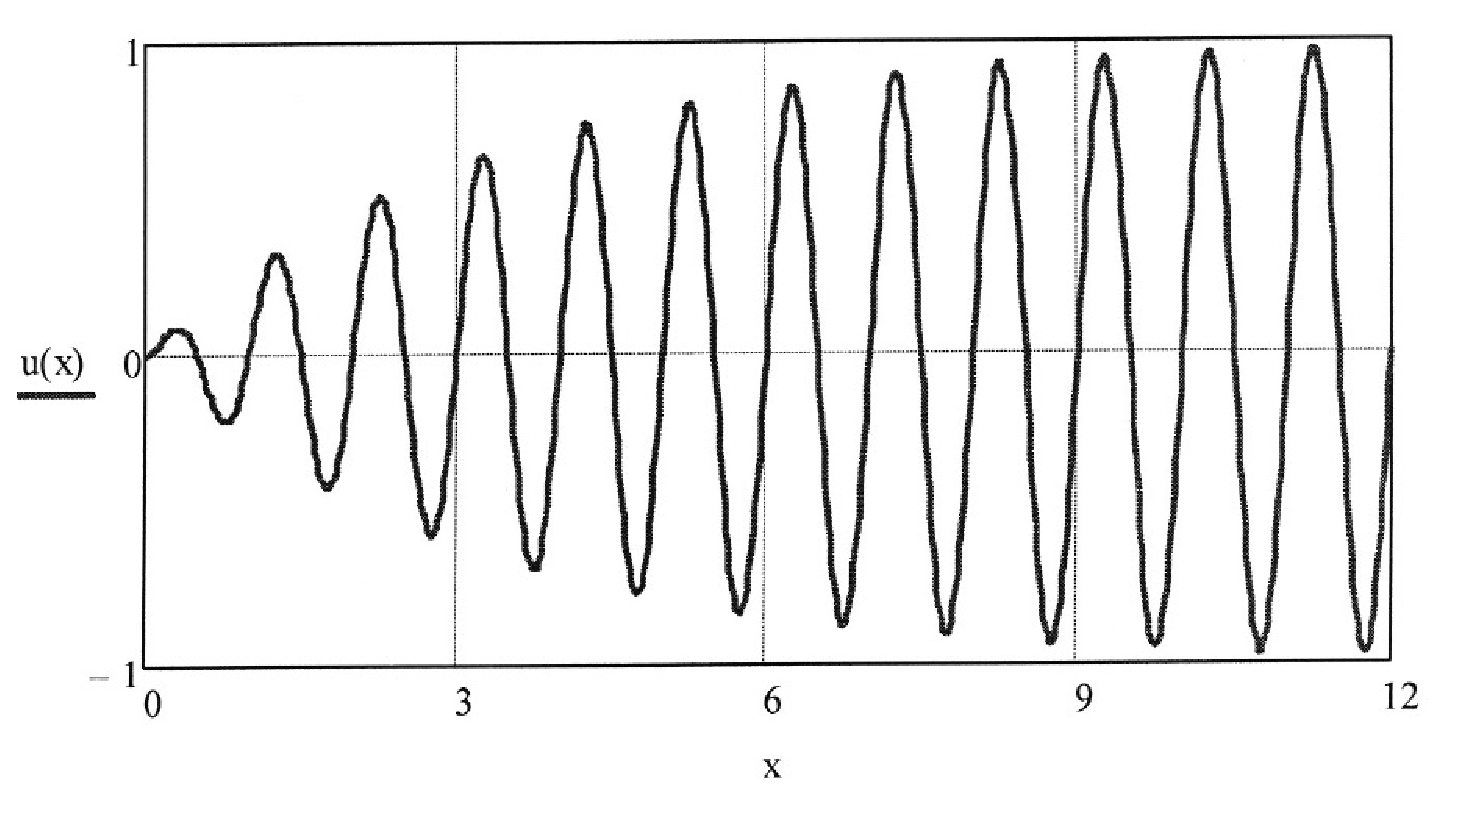
\includegraphics[width=0.6\linewidth]{Chapter_2/13}
	\caption{Установление колебаний вблизи резонанса $(|\Delta\omega|\ll\gamma=\delta\omega/2)$}
	\label{fig9}
\end{figure}

Рассмотрим два момента времени $t_1$ и $t_2,$ разделённые целым числом $n$ периодов $T_0.$ Амплиту\-ды колебаний $U_{Ck}(t_1)$ и $U_{C(k+n)(t_2)}$ при этом соответственно равны:
\begin{equation}\label{2.74}
U_{Ck}=U_0(1-e^{-\gamma t_1}),~~~~U_{C(k+n)}=U_0(1-e^{-\gamma(t_1+nT_0)}),~~~~U_0=Q\varepsilon_0.
\end{equation}
Из этих выражений находим логарифмический декремент
\begin{equation}\label{2.75}
\Theta=\dfrac{1}{n}\ln\dfrac{U_0-U_{Ck}}{U_0-U_{C(k+n)}}=\gamma T_0,
\end{equation}
а затем, измерив по осциллограмме реальный период $T_1\approx T_0,$ определяем коэффициент затуха\-ния $\gamma.$

Если расстройка $\Delta\omega$ удовлетворяет неравенствам $|\Delta\omega|\approx\gamma=\delta\omega/2\ll\omega_0,$ то есть расстройка сопоставима с шириной резонансной кривой, установление вынужденных колебаний на на\-чальной стадии процесса длительностью $\tau$ сопровождается биениями с частотой $|\Delta\omega|=|\omega-\omega_0|$ согласно уравнениям \eqref{2.72}. Вид колебаний в этом случае представлен на рис.\ref{fig10}.

\begin{figure}[h!]
	\centering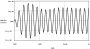
\includegraphics[width=0.6\linewidth]{Chapter_2/14}
	\caption{Биения при установлении колебаний $(\Delta\omega\approx\gamma=\delta\omega/2)$}
	\label{fig10}
\end{figure}

Амплитуда колебаний при этом то растёт, то падает, причём максимумы амплитуд постепенно уменьшаются. Лишь когда экспонента $e^{-\gamma t}$ достаточно затухнет, биения прекратятся, и колеба\-ния станут синусоидальными.
\begin{center}
СПИСОК ЛИТЕРАТУРЫ
\end{center}
 1. \emph{Сивухин Д.В.} Общий курс физики. –  Т. III, Электричество. \textbf{--} М.: Физматлит, 2006, §§122-124, 126, 127 129, 130.\\
2. \emph{Кингсепп А.С., Локшин Г.Р., Ольхов О.А.} Основы физики. Т.1. \textbf{--} М.: Физматлит, 2001,§§8.1-8.3.\\
3. \emph{Кириченко Н.А.} Электричество и магнетизм. \textbf{--} М.: МФТИ, 2011. Гл. 17.\\
4.\emph{ Горелик Г.С. Колебания и волны.} \textbf{--} М.: Физматлит, 1959. Гл. I, II, III.\\
5.\emph{ Гоноровский И.С.} Основы радиотехники. \textbf{--} М.: Связьиздат, 1957. Гл. 4. 


\newpage

\lab{Сдвиг фаз в цепи переменного тока}
\label{lab:phase}

\aim{изучить влияние активного сопротивления, индуктивности и ёмкости на сдвиг
фаз между током и напряжением в цепи
переменного тока.}

\equip{генератор звуковой частоты (ЗГ), двухканальный осциллограф (ЭО), магазин
ёмкостей, магазин сопротивлений, катушка
индуктивности, резисторы, универсальный измеритель импеданса ($LCR$-метр).}

Перед выполнением данной работы необходимо ознакомиться с теоретическим
введением к разделу (п. \ref{sec:forced}, \ref{sec:ures}).

Удобным, хотя и не очень точным, прибором для измерения фазовых соотношений 
служит электронный осциллограф. Можно предложить два способа измерения разности фаз.

В первом способе два сигнала~$U_1$ и~$U_2$ подаются 
на горизонтальную (канал~$X$) и вертикальную (канал~$Y$) развёртки осциллографа. 
Смещение луча по горизонтали и вертикали определяется выражениями
\begin{equation*}
x=x_0\cos\omega t,\qquad y=y_0\cos(\omega t+\psi),
\end{equation*}
где $\psi$~--- сдвиг фаз между напряжениями $U_1$ и $U_2$, а $x_0$ и~$y_0$~---
амплитуды напряжений, умноженные на
коэффициенты усиления соответствующих каналов осциллографа. Исключив время,
после несложных преобразований найдём
\begin{equation*}
\left(\frac{x}{x_0}\right)^2+ \left(\frac{y}{y_0}\right)^2+ \frac{2xy}{x_0 y_0}
\cos\psi=\sin^2 \psi.
\end{equation*}

\begin{wrapfigure}[13]{o}{0.45\linewidth}
	\pic{0.4\textwidth}{Chapter_2/2_1_1}
	\caption{Эллипс на экране осциллографа}
	\figmark{elips}
\end{wrapfigure}

Полученное выражение определяет эллипс, описываемый электронным лучом на 
экране осциллографа (рис.~\figref{elips}). Ориентация эллипса зависит как от искомого 
угла~$\psi$, так и от усиления каналов осциллографа. Для расчёта сдвига фаз 
можно измерить отрезки $2y_{x=0}$ и $2y_0$ (или $2x_{y=0}$ и $2x_0$, 
на рисунке не указанные) и, подставляя эти значения в уравнение эллипса, найти
\begin{equation}
\eqmark{phasexy}
\psi=\pm\arcsin\left(\frac{y_{x=0}}{y_0}\right).
\end{equation}
Для правильного измерения отрезка $2y_{x=0}$ важно, чтобы 
\emph{центр     эллипса лежал на оси~$y$}.

Второй способ заключается в непосредственном измерении сдвига 
фаз между сигналами на экране двухканального осциллографа.
Напряжения $U_1$ и $U_2$ одновременно подаются на входные каналы ЭО
при включённой внутренней горизонтальной развёртке. При этом
сигналы одновременно отображаются на экране.
Измерение разности фаз в таком случае удобно проводить следующим образом:
\begin{enumerate}[label=\arabic*),itemsep=0pt]
    \item подобрать частоту горизонтальной развёртки, при которой на экране 
    укладывается чуть больше половины периода синусоиды;
    \item отцентрировать горизонтальную ось;
    \item измерить расстояние $x_0$ (см. рис.~\figref{shift}) между нулевыми значениями 
    \emph{одного} из сигналов, что соответствует разности фаз $\pi$;
    \item измерить расстояние $x$ между нулевыми значениями двух синусоид 
    и пересчитать в сдвиг по фазе: $\psi=\pi x/x_0$. На рис.~\figref{shift} 
    синусоиды на экране ЭО сдвинуты по фазе на~$\pi/2$.
\end{enumerate}

\experiment 
Схема установки для исследования сдвига фаз между током и напряжением 
в цепи переменного тока представлена на рис.~\figref{shift}. Эталонная катушка~$L$, 
магазин ёмкостей~$C$ и магазин сопротивлений~$R$ соединены последовательно 
и через дополнительное сопротивление~$r$ подключены к источнику 
синусоидального напряжения~--- звуковому генератору (ЗГ).

\begin{figure}[hb]
    \centering\small
    \pic{0.8\textwidth}{Chapter_2/2_1_3}
    \caption{Схема установки для исследования сдвига фаз между током и
        напряжением}
    \figmark{shift}
\end{figure}

Сигнал, пропорциональный току, снимается c сопротивления~$r$, 
пропорциональный напряжению,~--- с генератора. Оба сигнала подаются 
на осциллограф (ЭО), имеющий два канала вертикального 
отклонения. Измерение разности фаз можно проводить одним из двух
описанных выше способов.

%, что позволяет одновременно наблюдать на экране два сигнала. 
%В нашей работе это две синусоиды, смещённые друг относительно друга 
%на некоторое расстояние, зависящее от сдвига фаз между 
%током и напряжением в цепи.


%\begin{wrapfigure}[13]{r}{0.45\linewidth}
%    \pic{0.4\textwidth}{Chapter_2/2_1_2}
%    \caption{Принципиальная схема фазовращателя}
%    \figmark{scheme}
%\end{wrapfigure}

На практике часто используются устройства, 
называемые \term{фазовращателями}, 
которые позволяют изменять фазу напряжения в широких пределах ($0<\psi<\pi$). 
Схема фазовращателя, применяемого в данной работе, 
изображена на рис.~\figref{rotator}. Она содержит два одинаковых 
резистора~$R_1$, смонтированных на отдельной плате,
магазин сопротивлений~$R$ и магазин ёмкостей~$C$. 

Найдём, как зависит сдвиг фаз между входным 
напряжением $U_{вх}=U_0\cos\omega t$ (точки~1 и~2 на рис.~\figref{rotator}) 
и выходным напряжением $U_{вых}$ (точки~3 и~4)
от соотношения между импедансами сопротивления~$R$ и ёмкости~$C$.
Для соответствующих комплексных амплитуд имеет место соотношение
(получите самостоятельно):
\begin{equation}
\eqmark{cplx}
\vec{U}_{вых}= \frac{\vec{U}_{вх}}{2}\dfrac{R+\frac{i}{\omega C}}{R-\frac{i}{\omega C}}.
\end{equation}
Числитель и знаменатель \eqref{cplx} --- комплексно-сопряжённые 
величины, модули которых одинаковы. Поэтому амплитуда выходного напряжения 
не зависит от~$R$, и всегда равна $U_{0}/2$.
Сдвиг фаз между выходным и входным напряжениями равен 
\begin{equation}
\eqmark{psi}
\psi = \arg \frac{\vec{U}_{вых}}{\vec{U}_{вх}} = 2\arctg \frac{1}{\omega RC}.
\end{equation}
Он может меняться от~$\psi=\pi$ при $R\to 0$ до~$\psi=0$ при $R\to\infty$.

\begin{figure}[h!]
    \centering
    \pic{0.8\textwidth}{Chapter_2/2_1_4}
    \caption{Схема установки для исследования фазовращателя}
    \figmark{rotator}
\end{figure}


\begin{lab:task}
\taskpreamble{В работе предлагается исследовать зависимости сдвига фаз между 
    током и напряжением от сопротивления в $RC$- и в $RL$-цепи; определить 
    добротность колебательного контура, сняв зависимость сдвига фаз от частоты 
    вблизи резонанса, определить диапазон работы фазовращателя.}

\tasksection{Исследование сдвига фаз в $RC$-цепи}

\item Ознакомьтесь с устройством используемых в работе приборов по техническому
описанию. Соберите схему согласно рис.~\figref{shift}.

\item В схеме, собранной по рис.~\figref{shift}, закоротите катушку, подключив оба провода, 
идущих к катушке, на одну клемму. Установите $C=0,5$~мкФ, $\nu=1$~кГц 
(см. рекомендации на установке) и 
рассчитайте реактивное сопротивление цепи $X_1=1/(\omega C)$
(циклическая частота $\omega=2\pi\nu$).

\item Увеличивая сопротивление $R$ от нуля до $\approx 10 X_1$, проведите 
измерения сдвига фаз $\psi$ для 6--8 значений $R$.
Предварительно подберите шаги $\Delta R$, для которых 
сдвиги синусоид на экране осциллографа $x$ (см. рис.~\figref{shift}) 
будут примерно равномерно лежать в диапазоне от~0 до~$x_0$. 

При изменениях параметров цепи периодически проверяйте положение 
нулевой линии синусоиды.

\tasksection{Исследование сдвига фаз в $RL$-цепи}

\item В схеме, собранной согласно \figref{shift}, закоротите магазин ёмкостей. 
Установите $L=50$~мГн, $\nu=1$~кГц (см. рекомендации на установке). 
Рассчитайте реактивное сопротивление цепи $X_2=\omega L$.

\item Меняя сопротивление $R$ от 0 до $\sim 10X_2$ 
(или до $R_{\rm max}$, указанного на установке), 
проведите измерения сдвига фаз $\psi$ для 6--8 значений $R$.

\tasksection{Исследование зависимости сдвига фаз от частоты в $RLC$-цепи}

\item В цепи, собранной согласно рис.~\figref{shift}, установите значения 
$R=0$, $L=50$~мГн, $C=0,5$~мкФ (см. рекомендации на установке). 
Рассчитайте резонансную частоту $\nu_0=1/(2\pi\sqrt{LC})$.
 
\item Подбирая частоту ЗГ, добейтесь резонанса. 
При резонансе должен наблюдаться нулевой сдвиг фаз $\psi=0$ (почему?).
При этом нулевые значения двух 
синусоид должны совместиться (а при равенстве амплитуд синусоиды 
полностью совпадают).
 
\item Меняя частоту \emph{в обе стороны} от резонансного значения, 
снимите зависимость сдвига фаз от частоты. С изменением частоты меняется 
расстояние $x_0$, которое занимает половина периода синусоиды, поэтому 
разумно каждый раз фиксировать отношение $x/x_0$. 
Вблизи резонанса ($|\psi|<\pi/3$) точки должны лежать чаще.
 
\item Повторите измерения для сопротивления $R=100$~Ом.
 
\item С помощью лабораторного $LCR$-метра измерьте сопротивление $r$,
а также индуктивность $L$ и активное сопротивление катушки $R_L$. 
Сравните измеренные значения с указанными на установке.


\tasksection{Исследование работы фазовращателя}

\item Соберите схему, изображённую на рис.~\figref{rotator}. Убедитесь, что 
выход ЗГ заземлён. Установите $C=0,5$~мкФ,  $\nu=1$~кГц
(см. рекомендации на установке). Оцените визуально диапазон изменения 
сдвига фаз при изменении $R$ от 0 до 10~кОм.
Подберите сопротивление $R$, при котором сдвиг фаз равен $\pi/2$.


\tasksection{Обработка результатов}

\item По результатам измерений сдвига фаз в $RC$-цепи постройте график
$\ctg\psi=f\left(\omega C R_{\Sigma}\right)$. Здесь $R_{\Sigma}=R+r$~--- 
суммарное активное сопротивление цепи. Получите теоретическую 
зависимость и изобразите её на том же графике. Проанализируйте
соответствие теории и результатов измерения.
%По графику определите значение $R$, при котором $\psi=\pi/2$ и сравните 
%результат с теоретическим.

\item Постройте график зависимости $\ctg\psi=f(R_{\Sigma}/\omega L)$ 
для $RL$-цепи (здесь $R_{\Sigma}=R+r+R_L$). Сравните график с теоретическим.

\item Постройте на одном листе графики $|\psi|=f(\nu/\nu_0)$ 
(фазово-частотные характеристики контура) для $R=0$ и~$100$~Ом (величину $\psi$ удобно откладывать в долях $\pi$).

Определите по графикам добротность контура: $Q=\nu_0/(2\Delta\nu)$, 
где $2\Delta\nu$~--- ширина графика при сдвиге фаз $\psi=\pi/4$.

\item Сравните добротность, определённую графически, с расчётом 
через параметры~$L$, $C$ и~$R$.

\item Постройте векторную диаграмму для фазовращателя; 
с её помощью рассчитайте сопротивление магазина $R$, при котором 
сдвиг фаз между входным и выходным напряжениями равен $\pi/2$. 
Сравните расчёт с измеренным значением.

%\n Сведите результаты эксперимента в таблицу:

\item Оцените погрешности измерений и 
сделайте выводы по результатам эксперимента.

\end{lab:task}


\begin{lab:questions}
	\item Что такое импеданс электрической цепи?
	Как складываются импедансы при последовательном и параллельном
соединении элементов?
    \item Получите формулу \eqref{phasexy} для измерения разности 
          фаз по форме эллипса.
    \item Получите выражение \eqref{cplx} для комплексной амплитуды напряжения на
    выходе фазовращателя.
    \item Дайте определение добротности колебательного контура.
    Опишите известные вам способы измерения добротности.
    \item Получите связь добротности $Q$ колебательного контура c шириной
    $\Delta \nu/\nu_0$ его фазово-частотной характеристики $\psi(\nu/\nu_0)$.
	%\item Можно ли описывать процессы затухания и установления колебаний,
%     пользуясь понятием импеданса?
    \item Как связаны фазы колебаний токов и напряжений 
    при резонансе а) в последовательном контуре, б) в параллельном контуре?
\end{lab:questions}


\begin{lab:literature}
	\item \SivuhinIII~--- \S~129, 130.
	\item \Kalashnikov~--- \S~220, 227, 228.
\end{lab:literature}

\lab{Резонанс напряжений в последовательном контуре}
\label{lab:322}

\begin{lab:aim}
исследование резонанса напряжений в последовательном колебательном контуре
с изменяемой ёмкостью, получение амплитудно-частотных и
фазово-частотных характеристик, определение основных параметров контура.
\end{lab:aim}

\begin{lab:equipment}
	генератор сигналов, источник напряжения, нагрузкой которого является
последовательный колебательный контур с переменной ёмкостью, двухканальный
осциллограф, цифровые вольтметры.
\end{lab:equipment}

%\begin{lab:warning}
% \warning{
Перед выполнением работы необходимо ознакомиться с основами теории электрических  
колебаний (см. введение п. \ref{sec:forced}, \ref{sec:ures}).
Необходимые  дополнения применительно к реальным элементам колебательного
контура будут приведены ниже.
%по вводной части Раздела II настоящего сборника и/или рекомендованной в нём
%литературе. 
% }
%\end{lab:warning}

\experiment

В данной работе изучаются резонансные явления в последовательном колебательном
контуре (резонанс напряжений). 
Схема экспериментального стенда показана на рис.~\figref{exp}.
Синусоидальный сигнал от генератора поступает на вход \important{управляемого
напряжением источника напряжения} (см., например, [3]), собранного на
операционном усилителе, питание которого осуществляется встроенным
блоком-выпрямителем от сети~$\sim220$~В (цепь питания на схеме не показана).
\emph{Источник напряжения} (источник с нулевым внутренним
сопротивлением) обеспечивает с высокой точностью постоянство
амплитуды сигнала~$\mathcal{E}=\mathcal{E}_0\cos(\omega t+\varphi_0)$ на
меняющейся по величине нагрузке~--- последовательном колебательном контуре,
изображенном на рис.~\figref{exp} в виде эквивалентной схемы. 

\begin{figure}[h!]
    \centering
	\pic{0.75\textwidth}{Chapter_2/2_2_2}
	\caption{Схема экспериментального стенда}
	\figmark{exp}
\end{figure}

Источник
напряжения, колебательный контур и блок питания заключены в отдельный корпус,
% с названием <<Резонанс напряжений>>, 
отмеченный на рисунке штриховой линией.
На корпусе имеются коаксиальные разъёмы <<Вход>>, <<$U_1$>> и <<$U_2$>>, а также
переключатель магазина ёмкостей $C_n$ с указателем номера $n=1,~2,~\ldots~7.$
Величины ёмкостей~$C_n$ указаны на установке. 
Напряжение~$\mathcal{E}$ на контуре через разъём <<$U_1$>> попадает одновременно 
на канал~1 осциллографа и вход 1-го цифрового вольтметра. Напряжение на конденсаторе~$U_C$ 
подаётся через разъём <<$U_2$>> одновременно на канал~2 осциллографа и
вход 2-го цифрового вольтметра.

\paragraph{Особенности реальных элементов цепи}
\label{par:real_elements}

Колебательный контур нашей установки собран из стандартных элементов,
используемых в современных радиоэлектронных цепях. Известно, что в реальных
конденсаторах и особенно в катушках индуктивности происходят 
\emph{необратимые потери} энергии, обусловленные различными причинами. К ним относятся: утечки и
диэлектрические потери в конденсаторах, вихревые токи и потери на
перемагничивание в сердечниках катушек индуктивности, омические потери в
проводниках, растущие с частотой за счёт скин-эффекта, и др. Рост
потерь приводит к увеличению действительных частей комплексных сопротивлений
элементов контура и, значит, к изменению его резонансных свойств, в частности,
к уменьшению добротности~$Q$.

Потери в элементах контура зависят как от частоты, так и от амплитуды тока
(напряжения), температуры и ряда других факторов, например, от вида диэлектрика
конденсатора, сердечника катушки и т.\,д. От перечисленных факторов в общем случае
зависят и основные параметры контура: индуктивность $L,$ ёмкость $C$ и суммарное
активное сопротивление~$R_{\Sigma}$.

В нашем контуре катушка индуктивности $L$ на ферритовом каркасе обладает малым
сопротивлением по постоянному току и высокой собственной резонансной
частотой~$\nu_{L0}\ge1,3$~МГц. В общем случае каждая катушка, помимо индуктивности~$L,$ характеризуется также собственной (межвитковой) ёмкостью $C_L$ и активным
сопротивлением потерь~$R_L,$ распределёнными по её длине. Принимается, что эти
величины сосредоточены в отдельных элементах схемы, образующих с индуктивностью~$L$ 
замкнутую колебательную цепь с собственной резонансной частотой
$\nu_{L0}=1/2\pi\sqrt{LC_L}.$ Вследствие влияния ёмкости~$C_L$ при измерении на
частоте~$\nu$ определяется не истинная индуктивность~$L,$ а эффективное значение
индуктивности $L_{эфф}=L/(1-\nu^2/\nu_0^2),$ которое может заметно отличаться от
истинной величины~$L.$ В рабочем диапазоне частот нашего контура выполняется
неравенство $\nu \ll \nu_0,$ так что в эквивалентной схеме контура на рис.~\figref{exp}
индуктивность представлена своим истинным значением~$L$ и активным
сопротивлением~$R_L.$

\begin{figure}[h!]
    \centering\small
    \pic{0.65\textwidth}{Chapter_2/2_2_3}
    \caption{Последовательная эквивалентная схема конденсатора с потерями}
    \figmark{equiv capacitor}
\end{figure}

Полипропиленовые конденсаторы с ёмкостями $C_n$ ($n=1\ldots7$), 
входящие в комплект магазина ёмкостей, в рабочем диапазоне частот имеют 
пренебрежимо малые собственные индуктивности (менее $10^{-5}$~мГн на~1~см 
общей длины обкладок и
выводов) и относительно малые активные потери. Для оценки возможного вклада
активных потерь в конденсаторах в общий импеданс контура воспользуемся
представлением конденсатора с ёмкостью~$C$ последовательной эквивалентной
схемой, показанной на рис.~\figref{equiv capacitor}а.
%\todo[author=Tiffani]{Нет рис 15 из ворд-файла в формате pic, проверить!}
На этой схеме $R_S$~---~так называемое \emph{эквивалентное последовательное
сопротивление} (ЭПС), обусловленное, главным образом, электрическим
сопротивлением материала обкладок и выводов конденсатора и контактов между ними,
а также потерями в диэлектрике. Из эквивалентной схемы и векторной диаграммы к
ней (рис.~\figref{equiv capacitor}б) видно, что активные потери в конденсаторе,
пропорциональные косинусу угла~$\varphi$ сдвига фаз между током и
напряжением на ёмкости, убывают с ростом~$\varphi$ и соответственно с
уменьшением угла $\delta=\frac{\pi}{2}-\varphi$. Потери в конденсаторе принято
характеризовать величиной $\tg\delta$, обычно приводимой в документации к
изделию. Из рис.~\figref{equiv capacitor} и закона Ома получаем 
выражение для ЭПС на циклической частоте $\omega=2\pi \nu$ в виде
\begin{equation}\eqmark{2.2.1}
R_S=\dfrac{U_{RS}}{I}=\dfrac{U_{RS}}{\omega CU_{CS}}=\dfrac{\tg\delta}{\omega C}.
\end{equation}
Конденсаторы магазина ёмкостей~$C_n$ в интересующем нас диапазоне частот имеют
$\tg\delta<10^{-3},$ что является очень хорошим (низким!) показателем для
конденсаторов с твёрдым диэлектриком.

\paragraph{Свойства колебательного контура}

В колебательный контур наших установок добавлен постоянный резистор $R$ (см.
рис.~\figref{exp}), снижающий его добротность. Это сделано для упрощения
процедур получения и обработки резонансных кривых. Таким образом, суммарное
активное сопротивление контура принимается равным
\begin{equation}\eqmark{2.2.2}
	R_{\Sigma}=R+R_L+R_S.
\end{equation}
Добротность контуров тем не менее остаётся достаточно высокой, чтобы можно
было пользоваться формулами \chaptereqref{2.35}, в которых
надо учитывать суммарное активное сопротивление контура:
\begin{equation}\eqmark{2.2.3}
	Q=\frac{\rho}{R_{\Sigma}}=\frac{\omega_0L}{R_{\Sigma}}=
    \frac{1}{\omega_0CR_{\Sigma}}\gg 1.
\end{equation}
Сильное неравенство в \eqref{2.2.3} в рабочем диапазоне частот выполняется для
всех контуров, используемых в работе.

Для импедансов ёмкости $Z_C$, индуктивности $Z_L$ и последовательного контура
$Z=Z_L+R+Z_C$ с учётом \eqref{2.2.1}, \eqref{2.2.2} получаем выражения
\begin{equation}\eqmark{2.2.4}
Z_C=R_S-\dfrac{i}{\omega C}, \qquad Z_L=R_L+i\omega L,\qquad
Z=R_{\Sigma}+i\left(\omega L-\dfrac{1}{\omega C}\right).
\end{equation}
Комплексные амплитуды тока в контуре~$\vec I=\vec E/Z$ и напряжений
на сопротивлении~$\vec{U}_{\! R}=R\vec I,$ ёмкости $\vec{U}_{\! C}=Z_C\vec I$ и
индуктивности $\vec{U}_{\! L}=Z_L\vec I$ при нулевой начальной фазе $\varphi_0$
напряжения на контуре $\vec{\mathcal{E}}=\mathcal{E}_0e^{i\varphi_0}$ 
по формулам~\chaptereqref{2.48a}, \chaptereqref{2.48b} 
с учётом \eqref{2.2.1}--\eqref{2.2.4} удобно записать в виде
%\begin{subequations}
%	\eqmark{2.2.5}
		\begin{equation}
			\eqmark{2.2.5a}
			\vec I=\dfrac{\vec
U_R}{R}=\dfrac{\mathcal{E}_0}{R_{\Sigma}}\dfrac{1}{
1+iQ(\omega/\omega_0-\omega_0/\omega)}, \end{equation}
		\begin{equation}
			\eqmark{2.2.5b}
			\vec
U_C=-iQ\mathcal{E}_0\dfrac{\omega_0}{\omega}\dfrac{1+i\tg\delta}{
1+iQ(\omega/\omega_0-\omega_0/\omega)},
		\end{equation}
		\begin{equation}
			\eqmark{2.2.5c}
			\vec
U_L=iQ\mathcal{E}_0\dfrac{\omega}{\omega_0}\dfrac{1-iR_L/\rho}{
1+iQ(\omega/\omega_0-\omega_0/\omega)}.
		\end{equation}
%\end{subequations}
Эти формулы уточняют результаты \chaptereqref{2.48a}--\chaptereqref{2.48b} и 
\chaptereqref{2.54a}--\chaptereqref{2.54d},
полученные без учёта потерь в конденсаторе и в катушке индуктивности. Отметим,
однако, что указанными потерями, представленными мнимыми добавками в числителях
формул~\eqref{2.2.5b} и~\eqref{2.2.5c}, при условиях $Q\gg1$ и
$\tg \delta \gg 10^{-3}$ можно пренебречь. В~то же время вклад этих потерь в
суммарное активное сопротивление контура $R_{\Sigma}$, вблизи
резонанса составляющий приблизительно $R_L+\rho\tg\delta$, 
можно оценить только по результатам эксперимента.

Основные особенности резонанса в последовательном контуре, называемого также
\important{резонансом напряжений} из-за увеличения в $Q$ раз напряжений на
ёмкости $U_C$ и индуктивности $U_L$ по отношению к внешнему напряжению
$\mathcal{E}_0,$ следуют из анализа формул \eqref{2.2.5a}--\eqref{2.2.5c}. 
Подробно этот вопрос рассматривался в п.~\ref{sec:ures} введения к разделу.
%\todo[author=Tiffani]{уточнить номер пункта (п.~3.1?)}

Наибольший практический интерес представляет случай, когда отклонение
$\delta\omega=\omega-\omega_0$ частоты внешней ЭДС от собственной частоты
контура $\omega_0$ удовлетворяет сильному неравенству
%\setcounter{equation}{5}
\begin{equation}\eqmark{2.2.6}
	|\Delta\omega| \ll \omega_0.
\end{equation}
При этом в первом порядке малости по относительной расстройке частоты
$\Delta\omega/\omega_0$
\begin{equation}\eqmark{2.2.7}
\dfrac{\omega}{\omega_0}-\dfrac{\omega_0}{\omega}=
\dfrac{2\Delta\omega}{\omega_0},
\end{equation}
что позволяет упростить выражения \eqref{2.2.5a}--\eqref{2.2.5c}
и представить вещественные части комплексных амплитуд 
и соответствующих им фаз в виде
\begin{align}
%	\eqmark{2.2.8}
%		\begin{equation}
			\eqmark{2.2.8a}
    	I & =\dfrac{U_R}{R}=\dfrac{\mathcal{E}_0}{R_{\Sigma}}
            \dfrac{\cos(\omega t-\psi_I)}{\sqrt{1+(\tau\Delta\omega)^2}}, &
        \psi_I &= \arctg (\tau\Delta\omega), \\
%		\end{equation}
%		\begin{equation}
			\eqmark{2.2.8b}
		U_C &= Q\mathcal{E}_0\dfrac{\omega_0}{\omega}
            \dfrac{\cos(\omega t-\psi_C)}{\sqrt{1+(\tau\Delta\omega)^2}}, &
        \psi_C &= \psi_I +\dfrac{\pi}{2}-\delta, \\
%		\end{equation}
%		\begin{equation}
			\eqmark{2.2.8c}
			U_L & =Q\mathcal{E}_0\dfrac{\omega}{\omega_0}
                \dfrac{\cos(\omega t-\psi_L)}{\sqrt{1+(\tau\Delta\omega)^2}}, &
        \psi_L & = \psi_I -\dfrac{\pi}{2}+\dfrac{R_L}{\rho}.
%		\end{equation}
\end{align}
Здесь $\tau$ --- время затухания \chaptereqref{2.24}. В выражениях \eqref{2.2.8b}, \eqref{2.2.8c} мы сохранили в прежнем виде
множители с отношениями частот в амплитудах и учли только линейные по малым
величинам $R_L/\rho$ и $\delta$ поправки в фазах, причём величину $\delta$
сохранили исключительно для общности, положив её константой.

При резонансе, когда для высокодобротного контура можно положить 
$\omega=\omega_0$ ($\Delta\omega=0$), 
выражения для модулей комплексных амплитуд тока и напряжения на ёмкости
и их фаз принимают вид (ср. \chaptereqref{2.61})
%и производных фаз по частоте $\omega$ принимают вид:
\begin{align}
%	\eqmark{2.2.9}
%		\begin{equation}
			\eqmark{2.2.9a}
		I(\omega_0) & =\dfrac{U_R}{R}=\dfrac{\mathcal{E}_0}{R_{\Sigma}}, &
        \varphi_I(\omega_0) & = 0, \\
%		\end{equation}
%		\begin{equation}
			\eqmark{2.2.9b}
		U_C(\omega_0) & = Q\mathcal{E}_0, &
            \psi_C(\omega_0) & = \dfrac{\pi}{2}-\delta; \\
        U_L(\omega_0) & = Q\mathcal{E}_0, &
            \psi_L(\omega_0) &=-\dfrac{\pi}{2}+\dfrac{R_L}{\rho}.
%		\end{equation}
%		\begin{equation}
%			\eqmark{2.2.9c}
%			\psi_I'(\omega_0)=\psi_C'(\omega_0)=\psi_L(\omega_0)=\tau.
%		\end{equation}
\end{align}
%Из формул \eqref{2.2.8}, \eqref{2.2.9} 
Из полученных соотношений следует, что на частоте $\omega_0,$ где
импеданс контура $Z$ становится чисто активным и равным $R_{\Sigma},$ амплитуда
тока достигает максимального значения $I_{\rm max}=\mathcal{E}_0/R_{\Sigma}.$
Напряжения $U_L$ и $U_C$ на индуктивности и ёмкости на частоте $\omega_0$
находятся почти в противофазе и в~$Q$ раз превышают по амплитуде напряжение
$\mathcal{E}$ внешней ЭДС. Напомним, однако, что максимальные (резонансные)
значения напряжений на индуктивности и ёмкости не
строго равны $Q\mathcal{E}_0$ и достигаются не строго на частоте $\omega_0$.
Соответствующие поправки, обусловленные множителями
$(\omega_0/\omega)^{\pm1}$ в амплитудах и малыми добавками к фазам в выражениях
для $U_C$ \eqref{2.2.8b} и $U_L$ \eqref{2.2.8c}, 
имеют порядок малости~$Q^{-2}$.
%\todo[author=Tiffani]{уточнить номер пункта (п.~3.1?)}

При отклонении $\Delta\omega$ частоты внешней ЭДС от $\omega_0$, таком, что
выполняется условие
%\setcounter{equation}{9}
\begin{equation}\eqmark{2.2.10}
\tau\Delta\omega=\pm1,
\end{equation}
амплитуда тока $I,$ как видно из \eqref{2.2.8a}, уменьшается в $\sqrt{2}$
раз относительно своей максимальной (резонансной) величины, а фаза $\psi_I$
изменяется на угол $\pm\pi/4$. 
В этой же точке, если не учитывать
поправки порядка $Q^{-1},$ происходят аналогичные изменения
амплитуд $U_C$, $U_L$ и фаз $\psi_C,~\psi_L$ напряжений на ёмкости и
индуктивности: амплитуды уменьшаются в $\sqrt{2}$ раз, а фазы меняются на угол
$\pm\pi/4$ по отношению к своим резонансным значениям.

Величина $\delta\omega=2|\Delta\omega|=2/\tau$ представляет собой важную
характеристику колебательного контура~--- \emph{ширину резонансной кривой}~$U_C(\omega)$
на уровне $U_C(\omega_0)/\sqrt{2}$, по которой можно определить
время затухания $\tau=2/\delta\omega$ и, зная резонансную частоту~$\omega_0$,
найти добротность контура $Q=\omega_0/\delta\omega$.

Эти же параметры можно определить по фазово-частотной характеристике: расстояние
по оси $\omega$ между точками, в которых фаза $\varphi_C$ меняется от $-\pi/4$
до $3\pi/4,$ согласно \eqref{2.2.8b} равно $2/\tau,$ а тангенс угла наклона
функции $\varphi_C(\omega)$ в точке резонанса согласно \chaptereqref{2.61c} определяет
время затухания~$\tau$.

В нашем эксперименте резонансные явления в последовательном колебательном
контуре исследуются по напряжению на контуре $\mathcal{E}$ и напряжению на
ёмкости $U_C$ (см. рис.~\figref{exp}), а также по фазовым сдвигам между ними.
%Приведённые выше формулы для других характеристик дополняют общую картину
%рассматриваемых процессов. В частности, они могут быть использованы для
%построения векторных диаграмм.

\begin{lab:task}

\item Проведите настройку экспериментального стенда по техническому описанию установки.
В двухканальном режиме работы осциллографа установите общее начало отсчёта $Y_1(t)$, $Y_2(t)$ вблизи левого края
средней линии экрана. В качестве синхронизующего сигнала выберите напряжение
$\mathcal{E}(t)$ при начальных условиях: $\mathcal{E}(0)=0,
\dot{\mathcal{E}}(0)<0.$

\item Установите на выходе генератора (на входе схемы) эффективное 
значение напряжения $\mathcal{E}$, указанное преподавателем 
(в пределах 30--300~мВ). Меняя частоту $\nu=\omega/2\pi$ генератора, 
убедитесь по осциллографу и вольтметрам, что у синусоиды $U_C(t)$ меняется амплитуда и фаза
относительно начала координат, тогда как синусоида
$\mathcal{E}(t)$~--- синхронизующий сигнал~--- <<привязана>> к началу отсчёта
при начальных условиях: $\mathcal{E}(0)=0, \dot{\mathcal{E}}(0)<0$, а её
амплитуда~$\mathcal{E}_0$ остаётся неизменной с относительной погрешностью не
менее $1\%$. 

\item Для контуров с 7 различными ёмкостями $C_n$, меняя их с помощью
переключателя на блоке, измерьте резонансные частоты $\nu_{0n}$ и напряжения
$U_C(\nu_{0n})$ при установленном в п.~2 напряжении~$\mathcal{E}$ на выходе
генератора. Регистрируйте также напряжения $\mathcal{E}(\nu_{0n})$, игнорируя
отклонения в пределах относительной погрешности~$1\%$. Приближение к резонансу
удобно наблюдать по фигуре Лиссажу на экране осциллографа в режиме $X$--$Y$.
При этом фигура Лиссажу представляет собой эллипс, оси которого на собственной
частоте~$\nu_{0n}$ направлены по~$X$ и~$Y$. 
Напомним, что максимальные значения напряжения~$U_C(\nu)$ достигаются на частотах, 
несколько отличных от собственных частот~$\nu_{0n}$.

    \item \footnote{Дополнительное упражнение, выполняется по указанию
        преподавателя.}Проделайте измерения п.~3 ещё
для двух напряжений $\mathcal{E}$ из интервала 30--300~мВ, существенно
отличающихся друг от друга и от напряжения, использованного в п.~3.

    \item Для контуров с двумя разными ёмкостями (по указанию преподавателя)
измерьте амплитудно-частотные характеристики $U_C(\nu)$ для значений
$U_C(\nu) \ge 0,6 U_C(\nu_{0n})$ (всего 16--18 точек по обе стороны от резонанса)
при том же напряжении~$\mathcal{E}$, что и в п.~3.

    \item Для тех же двух контуров измерьте фазово-частотные характеристики
$\psi_C(\nu)$ для значений $U_C(\nu)\ge0,3U_C(\nu_{0n})$ (всего 16--18 точек по
обе стороны от резонанса) при том же напряжении~$\mathcal{E},$ что и в п.~3.

Перед выполнением этого задания проверьте настройки осциллографа:
синхронизующий сигнал~$\mathcal{E}(t),$ как указано в п.~2, должен быть
<<привязан>> к общему началу отсчёта времени и напряжений на экране, лежащему на
оси~$X$ координатной сетки экрана. На той же оси должны располагаться нули
сигналов~$\mathcal{E}(t)$ и~$U_C(t)$. Если это не так, то следует повторить
процедуру центрирования горизонтальных осей каналов по техническому описанию.

Расстояние $x$ от начала отсчёта до точки первого обращения в нуль
напряжения $U_C(t)$ на участке спада характеризует разность фаз $\Delta\varphi$
сигналов $\mathcal{E}(t)$ и $U_C(t)$. Эта величина, выраженная в радианах,
даётся формулой $\Delta\varphi=\frac{x}{x_0}\pi$, где $x_0$~--- расстояние
от начала отсчёта до точки первого обращения в нуль напряжения $\mathcal{E}(t)$
на участке подъёма, соответствующее полупериоду этого сигнала.

\tasksection{Обработка и представление результатов}

% 		    \important{Настоятельно рекомендуется для обработки и представления
% результатов измерений использовать электронные таблицы.}

		    \item Результаты измерений п.~3 внесите в таблицу:\par
%		    \begin{center}
%		        \begin{table}[tb!]
		           % \caption{\eqmark{tab:1}
%		            \caption{}
%		            \tabmark{2.2.1}
%		            \begin{center}
\begingroup\small
\noindent\begin{tabular}{|c|c|c|c|c|c|c|c|c|c|c|} 
		                    \hline
		                    $C_n,$ & $f_{0n},$& $U_C,$& $\mathcal{E},$ & $L,$~&
$Q$& $\rho,$ & $R_{\Sigma},$~& $R_{S\text{max}},$& $R_L,$& $I,$\\

		                    нФ & кГц & В & В & мкГн &  & Ом & Ом & Ом & Ом & мА
\\
		                    \hline
		                    $C_1$ & & & & & & & & & & \\
		                    \hline
		                    $\cdots$ &  & & &  &  &  &  & & & \\
		                    \hline
		                    $C_7$& & & & & & & & & & \\
		                    \hline
		                    \multicolumn{4}{|c|}{Среднее значение} & & & & & & & \\
		                    \hline
		                    \multicolumn{4}{|c|}{Среднекв. отклонение} & & & & & & & \\ \hline
%		                    \multicolumn{4}{|c|}{Коэфф. Стьюдента} & & & & & & & \\
%		                    \multicolumn{4}{|c|}{$t_{n\alpha}$, $n=7$, $\alpha=0,05$} &
%& & & & & & \\ \hline
%		                    \multicolumn{4}{|c|}{для~$n=7,~\alpha=0,95$} &  & &
%& & && \\
%		                    \hline
%%		                    \multicolumn{4}{|c|}{ Коэффициент Стьюдента
%% $t_{n\alpha}$~для~$n=7,~\alpha=0,95$} & ---& & & & &---&\\
%%		                    \hline
%		                    \multicolumn{4}{|c|}{ Случайная погрешность } & ---&
%& & & &---&\\
%
		                    \multicolumn{4}{|c|}{Случ. погрешность} & & & & & & & \\ \hline
%		                    \hline
		                \end{tabular}
%		            \end{center}
%		        \end{table}
%		    \end{center}
\endgroup%\small

В первый столбец запишите значения ёмкостей~$C_n$,
приведённые в табличке на корпусе блока <<Резонанс напряжений>>. Для каждого
значения $C_n$ по формулам вводной части и данным эксперимента проведите
последовательно расчёт $L$, $Q$, $\rho$, $R_{\Sigma}$,
$R_{S\text{max}}=10^{-3}\rho$, $R_L$, $I$. Затем рассчитайте
средние значения $\left< L \right>$ и $\left< R_L \right>$ 
и их случайные погрешности ~$\Delta L$ и~$\Delta R_L$.

%Представьте результат проделанных в работе \important{косвенных
%измерений при невоспроизводимых условиях} величин $L$ и $R_L$ в виде: $\langle
%L\rangle\pm\Delta L$ и $\langle R_L\rangle\pm\Delta R_L,$ где угловыми скобками
%отмечены средние значения, а символом <<$\Delta$>>~--- случайные погрешности
%величин~$L$ и~$R_L$.

Оцените относительный вклад активных потерь в конденсаторах
(представленных в таблице сопротивлением $R_{S\text{max}}$, рассчитанным
для максимального значения $\tg\delta=10^{-3}$) в суммарное активное
сопротивление контура. Оцените влияние погрешностей приборов на результаты
измерений.

    \item *Выполните задание п.~7 для данных, полученных в п.~4. 
    Сравните с результатами п.~7. Объясните причины расхождения результатов, 
    если они обнаружатся.

    \item По данным измерений п.~5 постройте на одном графике
амплитудно-частотные характеристики $U_C(\nu)$ для выбранных
контуров. Проведите сравнительный анализ характеристик.

    \item По данным измерений п.~5 постройте на одном графике
амплитудно-частотные характеристики в безразмерных координатах 
$x\equiv \nu/\nu_{0n}$, $y\equiv U_C(x)/U_C(1)$. 
По ширине резонансных кривых на уровне $0,707$ определите добротности $Q$ 
соответствующих контуров. Оцените погрешности. 
Сравните эти величины с данными п.~7.

    \item По данным измерений п.~6 постройте на одном графике
фазово-частотные характеристики в координатах 
$x\equiv \nu/\nu_{0n}$, $y\equiv\varphi_C/\pi$ для выбранных контуров. 
По этим характеристикам определите
добротности контуров одним из двух способов: по расстоянию между точками по оси~$x$, 
в которых $y$ меняется от $1/4$ до $3/4$, равному $1/Q$, или по формуле
$Q=0,5\frac{d\varphi_C}{dx}$ при $x=0$. Оцените погрешности. 
Сравните с результатами п.~7,~10.

    \item Постройте зависимость $R_L(\nu_{0n})$ в системе координат с началом 
    в точке $(0,6\nu_{07};0);$ нанесите на график прямую $\langle R_L\rangle$. 
    Назовите возможные причины изменения $R_L$ с частотой.

    \item Постройте векторную диаграмму тока и напряжений для контура 
    с наименьшей добротностью в резонансном состоянии. Ось абсцисс направьте 
    по вектору $\vec{\mathcal{E}}$.

\end{lab:task}


\begin{lab:questions}
    \item Что такое импеданс электрической цепи?
    Как складываются импедансы при последовательном и параллельном
    соединении элементов?
    
     \item Дайте определение добротности колебательного контура.
     Опишите известные вам способы измерения добротности.
     
	\item Дайте энергетическое определение добротности колебательного контура.

	\item Объясните, почему оси эллипса на экране осциллографа (п.~3) при
условии $\omega=\omega_0$ ориентированы вдоль направлений X, Y.

	\item Как оценить добротность контура по векторной диаграмме в п.~13?

	\item По каким причинам потери в контуре зависят от частоты?

	\item *Зависит ли добротность контура от амплитуды сигнала, и если зависит,
то по каким причинам?

	\item *Получите выражение для частоты $\omega_m,$ на которой напряжение $U_C$
достигает максимума. Чему равна соответствующая амплитуда напряжения $U_C(\omega_m)$?
\end{lab:questions}


\begin{lab:literature}
    \item \SivuhinIII~--- \S~126, 127.
    \item \Kirichenko~--- \S~17.1--17.3.
	\item *\textit{Титце~У., Шенк~К.} Полупроводниковая схемотехника. Т.~II. ---
М.\,: ДМК Пресс,~2007.~--- \S~12.1.
\end{lab:literature}

\lab{Резонанс токов в параллельном контуре}

\begin{lab:aim}
	исследование резонанса токов в параллельном колебательном контуре с
изменяемой ёмкостью, получение амплитудно-частотных и
фазово-частотных характеристик, определение основных параметров контура.
\end{lab:aim}

\begin{lab:equipment}
	генератор сигналов, источник напряжения, нагрузкой которого является
параллельный колебательный контур с переменной ёмкостью, двухканальный
осциллограф, цифровые вольтметры.
\end{lab:equipment}

% \warning{
Перед выполнением работы необходимо ознакомиться с основами теории электрических  
колебаний (см. введение к разделу п. \ref{sec:forced}, \ref{sec:ires}).
Необходимые дополнения применительно к реальным элементам колебательного
контура будут приведены ниже.
% }

\experiment
В данной работе изучаются резонансные явления в параллельном колебательном
контуре (резонанс токов). Блок-схема экспериментального стенда 
показана на рис.~\figref{exp schem}. Синусоидальный сигнал
от генератора поступает на вход \important{управляемого напряжением источника
тока} (см., например, [3]), собранного на операционном усилителе с полевым
транзистором, питание которого осуществляется встроенным блоком-выпрямителем от
сети~$\sim220$~В (цепи питания на схеме не показаны).  Внутреннее (выходное)
сопротивление источника тока, бесконечно большое в идеальном случае, в нашей
схеме составляет несколько ГОм. Это обеспечивает постоянство амплитуды тока~$I$
на меняющейся нагрузке~--- параллельном контуре, изображенном на 
рис.~\figref{exp schem} в виде эквивалентной схемы.

\begin{figure}[h!]
    \centering
	\pic{0.68\textwidth}{Chapter_2/2_3_1}
	\caption{Блок-схема экспериментального стенда}
	\figmark{exp schem}
\end{figure}


Источник тока, колебательный контур и блок питания заключены в отдельный корпус,
%с названием <<Резонанс токов>> на верхней крышке, 
отмеченный на рисунке штриховой линией. 
На корпусе имеются коаксиальные разъёмы <<Вход>>,
<<${U}_1$>> и <<${U}_2$>>, а также переключатель магазина ёмкостей~$C_n$,
$n=1\ldots7$. Величины ёмкостей $C_n$ и сопротивления $R_1$ указаны на установке.
Напряжение $\mathcal{E}=\mathcal{E}_0\cos(\omega t+\varphi_0)$ от генератора поступает на
вход источника тока. Это же напряжение через разъём <<${U}_1$>> подаётся на
канал~1 осциллографа и на вход вольтметра~1. Переменное напряжение на
сопротивлении~$R_1$ в используемой схеме равно напряжению~$\mathcal{E}$ 
на выходе генератора и совпадает с ним по фазе. 
Cледовательно, ток $I$ во внешней цепи параллельного контура 
определяется формулами
\begin{equation}\eqmark{2.3.1}
	I=\frac{\mathcal{E}}{R_1}=I_0\cos(\omega t+\varphi_0), \qquad 
    I_0=\frac{\mathcal{E}_0}{R_1}.
\end{equation}

Напряжение на контуре $U$, совпадающее с напряжением на конденсаторе $U_C$,
поступает \emph{со знаком} <<$–$>> через разделительный конденсатор и разъём
<<${U}_2$>> на канал~2~осциллографа, а также на вход вольтметра~2.


Колебательный контур нашей установки собран из стандартных элементов,
используемых в современных радиоэлектронных цепях. Характеристики реальных элементов
представлены в описании работы \ref{lab:322}. \emph{Для понимания дальнейшего
изложения читателю рекомендуется ознакомиться с разделом
<<Особенности реальных элементов цепи>> на стр.~\pageref{par:real_elements}.} 
С учётом приведённых в указанном материале результатов получаем выражения
для импедансов ёмкостной $Z_C$ и индуктивной $Z_L$ ветвей параллельного 
колебательного контура:
\begin{equation}\eqmark{2.3.2}
	Z_C=R_S-\dfrac{i}{\omega C}, \qquad Z_L=R+R_L+i\omega L,
\end{equation}
где $R_S\equiv\dfrac{\tg\delta}{\omega C}$ и $R_L$~--- активные части
импедансов конденсатора и катушки индуктивности соответственно, а $R$~--- величина
постоянного активного сопротивления, добавленного в индуктивную ветвь
колебательного контура для снижения его добротности с целью упрощения  процедур
получения и обработки резонансных кривых. 
Конденсаторы магазина ёмкостей~$C_n$ в интересующем нас диапазоне
частот имеют относительно малые потери: для них $\tg\delta<10^{-3}.$

Добротность $Q$ контуров в наших установках достаточно высока, поэтому
можно пользоваться формулами \chaptereqref{2.34} и \chaptereqref{2.64}, в
которых, однако, надо учитывать, что суммарное активное сопротивление контура в
этом случае даётся формулой
\begin{equation}\eqmark{2.3.3}
	R_{\Sigma}=R+R_L+R_S
\end{equation}
и, следовательно,
\begin{equation}\eqmark{2.3.4}
	Q=\frac{\rho}{R_{\Sigma}}=
    \frac{\omega_0 L}{R_{\Sigma}}=
    \frac{1}{\omega_0 CR_{\Sigma}} \gg 1.
\end{equation}
Сильное неравенство \eqref{2.3.4} в рабочем диапазоне частот выполняется для
всех контуров, используемых в работе.

\important{Комплексные амплитуды} токов в ёмкостной $\vec{I}_{\! C}$ и индуктивной
$\vec{I}_{\! L}$ ветвях контура, а также напряжения $\vec U$ на контуре, положив без
ограничения общности $\varphi_0=0$ в выражении для внешнего тока $\vec
I=I_0e^{i\varphi_0}$ и используя формулы \chaptereqref{2.64} с учётом
\eqref{2.3.1}–-\eqref{2.3.4}, удобно представить в виде
\begin{align}
%	\eqmark{2.3.5}
%		\begin{equation}
			\eqmark{2.3.5a}
			\vec{I}_{\! C} &= \vec{I}\dfrac{Z_{LR}}{Z_C+Z_{LR}}=
                iQI_0\dfrac{\frac{\omega}{\omega_0}-i \frac{R+R_L}{\rho}}{%
                        1+iQ(\frac{\omega}{\omega_0}-\frac{\omega_0}{\omega})}, \\
%		\end{equation}
%		\begin{equation}
			\eqmark{2.3.5b}
			\vec{I}_{\! L}&=\vec{I}\dfrac{Z_C}{Z_C+Z_LR}=
                -iQI_0\dfrac{\frac{\omega_0}{\omega}(1+\tg\delta)}{%
                    1+iQ(\frac{\omega}{\omega_0}-\frac{\omega_0}{\omega})}, \\
%		\end{equation}
%		\begin{equation}
			\eqmark{2.3.5c}
			\vec U&=\vec{I}\dfrac{Z_C Z_LR}{Z_C+Z_LR}= 
                Q\rho I_0 \dfrac{[1-i\frac{\omega_0}{\omega}\frac{R+R_L}{\rho}](1+i\tg\delta)}{%
                    1+iQ(\frac{\omega}{\omega_0}-\frac{\omega_0}{\omega})}.
%		\end{equation}
\end{align}
Из формул \eqref{2.3.5b}, \eqref{2.3.5c} следует, что потерями в конденсаторах,
явно представленных величиной $\tg\delta<10^{-3}$, можно пренебречь. 
В~то же время необходимость учёта вклада этих потерь в
суммарное активное сопротивление контура~$R_{\Sigma}$ 
вблизи резонанса, примерно равного $\rho\tg\delta,$ можно будет оценить только по
результатам эксперимента.

Наибольший практический интерес для контуров с \important{высокой добротностью}
($Q\gg1$) представляет случай, когда отклонение $\Delta\omega=\omega-\omega_0$ частоты
внешней ЭДС от собственной частоты контура удовлетворяет сильному неравенству
\begin{equation}\eqmark{2.3.6}
|\Delta\omega|\ll \omega_0.
\end{equation}
При этом в первом порядке малости по относительной расстройке частоты 
$\frac{\Delta\omega}{\omega_0}$ выполняется соотношение
\begin{equation}\eqmark{2.3.7}
\frac{\omega_0}{\omega_0}-\frac{\omega}{\omega}\approx\frac{2\Delta\omega}{\omega_0},
\end{equation}
которое позволяет упростить выражения \eqref{2.3.5a}--\eqref{2.3.5c} 
и представить вещественные части комплексных амплитуд в виде
\begin{align}
%	\eqmark{2.3.8}
%		\begin{equation}
			\eqmark{2.3.8a}
			I_C(t) &= QI_0\dfrac{\omega}{\omega_0}
                \dfrac{\cos(\omega t-\psi_C)}{R\sqrt{1+(\tau\Delta\omega)^2}}, &
            \psi_C &=
                \arctg(\tau\Delta\omega)-\dfrac{\pi}{2}+\dfrac{R+R_L}{\rho}, \\
%		\end{equation}
%		\begin{equation}
			\eqmark{2.3.8b}
			I_L(t) &= QI_0\dfrac{\omega_0}{\omega} 
                \dfrac{\cos(\omega t-\psi_L)}{\sqrt{1+(\tau\Delta\omega)^2}}, &
            \psi_L &= \arctg(\tau\Delta\omega)+\dfrac{\pi}{2}-\delta, \\
%		\end{equation}
%		\begin{equation}
			\eqmark{2.3.8c}
			U(t) &= Q\rho I_0 \dfrac{\cos(\omega t-\psi_U)}{% 
                \sqrt{1+(\tau\Delta\omega)^2}}, &
            \psi_U &=\arctg(\tau\Delta\omega)+
                \dfrac{\omega_0}{\omega}\dfrac{R+R_L}{\rho}-\delta,
%		\end{equation}
\end{align}
%$$
%	I_C(t)=QI_0\dfrac{\omega}{\omega_0}\dfrac{\cos(\omega
% t-\psi_C)}{R\sqrt{1+(\tau\Delta\omega)^2}},~~~~
%	\psi_C=\arctg(\tau\Delta\omega)-\dfrac{\pi}{2}+\dfrac{R+R_L}{\rho},
% \eqno{(8a)}
%$$
%$$
%	I_L(t)=
%	QI_0\dfrac{\omega_0}{\omega}
%	\dfrac{\cos(\omega
% t-\psi_L)}{\sqrt{1+(\tau\Delta\omega)^2}},
% ~~~~\psi_L=\arctg(\tau\Delta\omega)+\dfrac{\pi}{2}-\delta, \eqno{(8\text{б})}
%$$
%$$
%	U(t)=
%	Q\rho I_0
%	\dfrac{\cos(\omega t-\psi_{{U}})}
%	{\sqrt{1+(\tau\Delta\omega)^2}},~~~~
%
% \psi_{{U}}=\arctg(\tau\Delta\omega)+\dfrac{\omega_0}{\omega}\dfrac{R+R_L}{\rho}
% -\delta \eqno{(8\text{в})}
%$$
где $\tau=2L/R_{\Sigma}=2Q/\omega_0$ --- время затухания
колебательного контура. В выражениях \eqref{2.3.8a}--\eqref{2.3.8c} 
мы сохранили в прежнем виде множители с отношениями частот в амплитудах и учли только линейные по малым
величинам $(R~+~R_L)/\rho$ и $\delta$ поправки в фазах, причём величину $\delta$
сохранили исключительно для общности, полагая её, однако, константой.

Как видно из выражений \eqref{2.3.8a}--\eqref{2.3.8c}, 
вблизи частоты~$\omega_0$ зависимости амплитуд токов и напряжения на контуре 
от частоты~$\omega$ несколько различаются, что надо иметь в виду при экспериментальном 
исследовании резонанса токов \important{по напряжению на контуре}~$U.$

Отдельно обратим внимание на тот факт, что зависимость \eqref{2.3.8c} амплитуды
напряжения $U$ на параллельном контуре от частоты $\omega$ вблизи резонанса в
принятом приближении совпадает с аналогичной зависимостью \chaptereqref{2.60b}
амплитуды тока $I_{\omega}$ для последовательного контура в том же приближении.

В резонансе, когда для высокодобротного контура можно положить
$\omega=\omega_0$, амплитуды токов и напряжения \eqref{2.3.8a}--\eqref{2.3.8c}
и их фазы 
%и производная фазы $\psi_U$ по частоте $\omega$ 
принимают вид
\begin{equation}
	\eqmark{2.3.9}
    \begin{aligned}
%			\eqmark{2.3.9a}
			 I_C(\omega_0) & = QI_0, & 
                 \psi_C(\omega_0) & = -\dfrac{\pi}{2}+Q^{-1}-\tg\delta, \\
			 I_L(\omega_0) & = QI_0, & \psi_L(\omega_0) & =
                 \dfrac{\pi}{2}-\delta, \\
%			\eqmark{2.3.9b}
			U(\omega_0) &= Q\rho I_0, & \psi(\omega_0) & = 
                    Q^{-1}-\tg\delta-\delta.
%                    \qquad \psi'_U(\omega_0)=\tau.
    \end{aligned}
\end{equation}
%$$
%	I_C(\omega_0)=
%	QI_0,~~\psi_C(\omega_0)=
%	-\dfrac{\pi}{2}+Q^{-1}-\tg\delta,~~~~~~
%	I_L(\omega_0)=
%	QI_0,~~
%	\psi_L(\omega_0)=
%	\dfrac{\pi}{2}-\delta, \eqno{(9a)}
%$$
%$$
%	U(\omega_0)=
%	Q\rho I_0,~~~~
%	\psi(\omega_0)=
%	Q^{-1}-\tg\delta-\delta,~~~~
%	\psi'_{{U}}(\omega_0)=\tau. \eqno{(9\text{б})}
%$$
%\setcounter{equation}{9}
В последнем равенстве мы пренебрегли относительными поправками порядка $Q^{-2}$
и $Q^{-1}\tg\delta$. Из формул \eqref{2.3.9} следует, что на частоте $\omega_0$
токи $\vec{I}_{\! C}$ и~$\vec{I}_{\! L}$ в ёмкостной и индуктивной ветвях контура в~$Q$ раз
превышают по амплитуде ток~$\vec{I}$ во внешней цепи. При этом ток~$\vec{I}_{\! C}$
опережает внешний ток~$\vec{I}$ по фазе почти на $\pi/2$, 
а ток~$\vec{I}_{\! L}$ отстаёт от~$\vec{I}$ почти на~$\pi/2$. 
Между собой токи~$\vec{I}_{\! C}$ и~$\vec{I}_{\! L}$ сдвинуты по фазе на угол, 
близкий к  $\pi.$ Можно сказать, что токи $\vec{I}_{\! C}$ и $\vec{I}_{\! L}$ 
образуют контурный ток, последовательно обтекающий элементы контура и 
в~$Q$ раз превышающий внешний ток $\vec{I}$. Именно
последнее обстоятельство послужило поводом назвать резонанс в 
параллельном контуре <<резонансом токов>>.

Отметим также, что максимальные (резонансные) значения токов в контуре 
не строго равны $QI_0$ и достигаются не строго на частоте $\omega_0$.
Соответствующие относительные поправки составляют доли малой 
величины $Q^{-2}$ и связаны с входящим в выражения 
\eqref{2.3.8a}, \eqref{2.3.8b} для вещественных амплитуд 
токов $\vec{I}_{\! C}$, $\vec{I}_{\! L}$ множителем $\frac{\omega}{\omega_0}$.

Из формул \eqref{2.3.9} вытекает, что на частоте $\omega_0$ импеданс контура
$Z(\omega_0)=\vec U(\omega_0)/I_0$ является почти чисто активным. В~пренебрежении 
относительными поправками порядка $Q^{-2}$ его модуль и фаза относительно внешнего 
тока определяются формулами
\begin{equation}\eqmark{2.3.10}
|Z(\omega_0)|=Q\rho=Q^2R_{\Sigma}, \qquad
\psi_Z(\omega_0)=\dfrac{R+R_L}{\rho}-\delta,
\end{equation}
которые дополняют формулы \chaptereqref{2.67} учётом активных потерь в катушке
индуктивности и в конденсаторе.

При отклонении $\Delta\omega$ частоты внешней ЭДС от частоты $\omega_0$, таком,
что выполняется условие
\begin{equation}\eqmark{2.3.11}
\tau\Delta\omega=\pm1,
\end{equation}
амплитуда напряжения $U,$ как видно из формул \eqref{2.3.8c}, уменьшается в
$\sqrt{2}$ раз относительно своей резонансной величины, а фаза $\psi_U$
изменяется примерно на угол $\pm\pi/4.$
Величина $\delta\omega\equiv2|\Delta\omega_{\gamma}|=2\gamma=2/\tau$
представляет собой важную характеристику колебательного
контура~---~\important{ширину резонансной кривой} $U(\omega),$ по которой с
учётом соотношений $Q=\omega_0/2\gamma=\tau\omega_0/2,$ зная частоту $\omega_0,$
можно найти добротность контура: 
\begin{equation}\eqmark{2.3.12}
Q=\dfrac{\omega_0}{\delta\omega}.
\end{equation}

Эти же параметры можно определить по фазово-частотной характеристике: тангенс
угла наклона $\psi_U$ в точке $\omega=\omega_0$ согласно \chaptereqref{2.66c}
определяет время затухания $\tau,$ а расстояние по оси $\omega$ между точками, в
которых фаза $\psi_U(\omega)$ меняется от $-\pi/4$ до $\pi/4,$ равно $2/\tau$ с
относительной погрешностью порядка $Q^{-2}.$

\begin{lab:task}
    \item Проведите настройку экспериментального стенда по техническому описанию
установки.

    \item Меняя частоту $\nu$ генератора, убедитесь по осциллографу и вольтметрам,
что у синусоиды $U(t)$ меняется амплитуда и фаза относительно начала координат,
тогда как синусоида $\mathcal{E}(t)$~---~синхронизующий сигнал~---~<<привязана>>
к началу отсчёта при начальных условиях: $\mathcal{E}(0)=0$,
$\dot{\mathcal{E}}(0)=0$, а её амплитуда остаётся неизменной с относительной
погрешностью  $\le1\%$. После этого можно приступить к измерениям.

    \item Для контуров с семью различными ёмкостями $C_n$, меняя их с помощью
переключателя на блоке, измерьте резонансные частоты~$\nu_{0n}$ и напряжения
$U(\nu_{0n})$. Регистрируйте для контроля также напряжения~$\mathcal{E}$,
игнорируя отклонения в пределах относительной погрешности~$1\%$. Состояние
резонанса определяйте по максимуму напряжения $U(\nu_{0n})$, измеряемого
вольтметром и наблюдаемого на экране осциллографа. Приближение к резонансу
удобно наблюдать по фигуре Лиссажу на экране осциллографа в режиме $X$--$Y$.
При этом фигура Лиссажу представляет собой эллипс, вырождающийся в прямую линию
с положительным наклоном \important{почти} на частоте $\nu_{0n}$.

    \item \footnote{Дополнительное упражнение, выполняется по указанию
        преподавателя.}Проделайте измерения п.~3 для напряжения, существенно 
    отличающегося от использованного в п.~3, но лежащего в диапазоне $100\div500$~мВ 
    по амплитуде.

    \item Для контуров с двумя разными ёмкостями (по указанию преподавателя)
снимите амплитудно-частотные характеристики $U(f)$ для значений
$U(f)\ge0,6U(\nu_{0n})$ (всего 16--18 точек по обе стороны от резонанса) при
том же напряжении $\mathcal{E}$, что и в п.~3.

    \item Для тех же двух контуров измерьте фазово-частотные характеристики
$\psi_U(f)$ для значений $U(f)\ge0,3U(\nu_{0n})$ (всего 16--18 точек по обе
стороны от резонанса) при том же напряжении, что и в п.~3. Перед выполнением
этой части работы измените с помощью ручек горизонтальной развёртки настройки
осциллографа таким образом, чтобы синхронизующий сигнал $\mathcal{E}(t)$ был
<<привязан>> к общему началу отсчёта времени и напряжений на экране, лежащему на
оси X координатной сетки экрана (см. п.~2), и оба сигнала были симметричны
относительно этой оси. Если это не так, то следует повторить процедуру
центрирования горизонтальных осей каналов по техническому описанию.

    Расстояние $x$ от начала отсчёта до точки первого обращения в нуль
напряжения $U(t)$ на участке спада на осциллограмме характеризует разность фаз
$\Delta\varphi$ сигналов $U(t)$ и $\mathcal{E}(t).$ Эта величина, выраженная в
радианах, очевидно, даётся формулой $\Delta\varphi=\frac{x}{x_0}\pi$, где
$x_0$~--- расстояние от начала отсчёта до точки первого обращения в нуль
напряжения~$\mathcal{E}(t)$ на участке подъёма, соответствующее полупериоду
этого сигнала.

	\tasksection{Обработка и представление результатов}
% 	\important{Настоятельно рекомендуется для обработки и представления
% результатов измерений использовать электронные таблицы.}

	\item Результаты измерений п.~3 внесите в таблицу:\par
%	    \begin{table}[h!]
	        %\caption{\label{tab:1}}
%	        \caption{}
%	        \tabmark{2.3.1}
%	        \begin{center}
\begingroup
\noindent\small \begin{tabular}{|c|c|c|c|c|c|c|c|c|c|c|}
	                \hline
	                $C,$ & $f,$ & $U,$ & $\mathcal{E},$ & $L,$ &
$\rho,$ & $|Z_{\text{рез}}|,$& $Q$ & $R_{\Sigma},$ & $R_{S
\text{max}},$& $R_L,$\\

	                нФ & кГц & В & В & мкГн & Ом & Ом &  & Ом & Ом & Ом \\
	                \hline
	                $C_1$ & --- & --- & --- & --- & --- & --- & --- & --- & --- & --- \\
	                \hline
	                $\cdots$ & --- & --- & --- & --- & --- & --- & --- & ---& --- & --- \\
	                \hline
	                $C_7$& --- & --- & --- & --- & --- & --- & ---& --- &--- &---\\
	                \hline
	                \multicolumn{4}{|c|}{Среднее значение} & --- & & & & & & --- \\
	                \hline
%	                \multicolumn{4}{|c|}{Среднекв. отклонение} & ---& & & & & &--- \\
%			                    \hline
%\multicolumn{4}{|c|}{Коэфф. Стьюдента} & & & & & & & \\
%\multicolumn{4}{|c|}{$t_{n\alpha}$, $n=7$, $\alpha=0,05$} & & & & & & & \\ \hline
	                \multicolumn{4}{|c|}{Случ. погрешность} & ---& & & & & &---\\
	                \hline
	            \end{tabular}\par
\endgroup

В первый столбец этой таблицы запишите значения ёмкостей $C_n$. 
Для каждого значения $C_n$ по формулам вводной части и данным 
эксперимента проведите \important{последовательно} расчёт~$L$, 
$\rho$, $|Z_{\text{рез}}|$, $Q$, $R_{\Sigma}$, 
$R_{S \text{max}}=10^{-3}\rho$, $R_L$.
Затем рассчитайте средние значения $\left< L \right>$ и $\left< R_L \right>$ 
и их случайные погрешности~$\Delta L$ и~$\Delta R_L$
как среднеквадратичные отклонения соответствующих величин.

%Представьте результат \important{косвенных измерений при невоспроизводимых
%условиях,} проделанных в работе, в виде: $\langle L \rangle\pm\Delta L$ и
%$\langle R_L\rangle\pm\Delta R_L,$ где угловыми скобками отмечено среднее
%значение, а символом $"\Delta"$ – случайная погрешность величин $L$ и $R_L.$

Оцените относительный вклад активных потерь в конденсаторах 
(представленных в таблице сопротивлением $R_{S\text{max}}$, рассчитанным для
максимального значения $\tg\delta=10^{-3}$) в суммарное активное сопротивление
контура.

\item *Выполните задание п.~7 для данных,
полученных в п.~4. Сравните с результатами п.~7. Объясните причины расхождения
результатов, если они обнаружатся.

\item По данным измерений п.~5 постройте на одном графике амплитудно-частотные
характеристики $U(\nu)$  для выбранных контуров. Проведите сравнительный 
анализ характеристик.

\item По данным измерений п.~5 постройте на одном графике амплитудно-частотные
характеристики в безразмерных координатах $x\equiv \nu/\nu_{0n}$, $y\equiv
U(x)/U(1).$ По ширине резонансных кривых на уровне 0,707 определите добротности
$Q$ соответствующих контуров. Оцените погрешности. Сравните эти величины с
расчётами п.~7.

\item По данным измерений п.~6 постройте на одном графике фазово-частотные
характеристики $\psi_U(\nu)$ в координатах $x\equiv \nu/\nu_{0n}$, $y\equiv\psi_U/\pi$
для выбранных контуров. По этим характеристикам определите добротности контуров
одним из двух способов: по формуле $Q=\frac12 \frac{d\varphi_U(x)}{dx}$ при $x=1$ или по
расстоянию $1/Q$ между точками оси $x,$ в которых  меняется от $-1/4$ до $1/4$. 
Оцените погрешности. Сравните с результатами п.~7 и~10.

\item Постройте зависимость $R_L(\nu_{0n})$ в системе координат с началом 
в точке $(0,6\nu_{07};0)$, нанесите на график прямую $\langle R_L \rangle$. 
Назовите возможные причины изменения~$R_L$ с частотой.

\item Постройте векторную диаграмму токов и напряжений для контура 
с наименьшей добротностью в резонансном состоянии. Ось ординат направьте по 
вектору $\vec{I}$.
\end{lab:task}


\begin{lab:questions}
    \item Что такое импеданс электрической цепи?
    Как складываются импедансы при последовательном и параллельном
    соединении элементов?
    
    \item Дайте определение добротности колебательного контура.
    Опишите известные вам способы измерения добротности.
    
    \item Дайте энергетическое определение добротности колебательного контура.

    \item  Получите выражение для напряжения на катушке индуктивности  в
резонансе.

    \item Дайте обоснование способам определения добротности по
фазово-частотной характеристике.

    \item По каким причинам потери в контуре зависят от частоты?

    \item *Зависят ли потери в контуре от амплитуды сигнала, и если зависят, то
по каким причинам?

    \item *Оцените, на какой частоте $\omega_m$ эллипс на экране осциллографа в
п.~3 вырождается в прямую линию с положительным наклоном.
\end{lab:questions}


\begin{lab:literature}
        \item \SivuhinIII~--- \S~126, 127.
        \item \Kirichenko~--- \S~17.1--17.3.
    \item *\emph{Титце~У., Шенк~К.} Полупроводниковая схемотехника.  --- Т.~II. ---
Москва\,: ДМК~Пресс, 2007.~--- \S~12.1.
\end{lab:literature}


\lab{Свободные колебания в электрическом контуре}

\begin{lab:aim}
исследование свободных колебаний в колебательном контуре.
\end{lab:aim}

\begin{lab:equipment}
генератор импульсов, электронное реле, магазин сопротивлений, магазин ёмкостей, катушка индуктивности, электронный осциллограф, универсальный мост.
\end{lab:equipment}

Исследуемый колебательный контур состоит из индуктивности $L$, ёмкости $C$ и резистора $R$ (рис.~\figref{fig1}). Конденсатор контура заряжается короткими одиночными импульсами, после каждого из которых в контуре возникают свободные затухающие колебания. Подав напряжение с конденсатора на осциллограф, можно по изображению на экране осциллографа определить период свободных колебаний в контуре, исследовать их затухание и определить основные параметры колебательного контура.

%\begin{figure}[h]
\begin{wrapfigure}[13]{r}{0.45\linewidth}
	\pic{0.4\textwidth}{Chapter_2/2_4_1}
	\caption{Схема установки для наблюдения затухающих колебаний на фазовой плоскости}
	\figmark{dumped oscillations}
\end{wrapfigure}
%\end{figure}

Картину колебаний можно представить не только в координатах ($U$,~$t$) (рис.~\figref{fig2}а), но и в координатах ($U$,~$U̇$)~---~на так называемой \important{фазовой плоскости} (рис.~\figref{fig2}б). В этих координатах кривая незатухающих колебаний (при $\gamma~=~0$) имеет вид эллипса, а картина реальных затухающих колебаний представляет собой сворачивающуюся спираль.
\todo[author=Tiffani]{Проверить на ошибку. Скорее всего в координатах (U, I), а не (U, U)}

Принципиальная схема подключения осциллографа для изучения колебаний на фазовой плоскости изображена на рис.~\figref{dumped oscillations}. На вертикальный вход осциллографа подаётся напряжение $U_C$ с конденсатора, а на горизонтальный~---~напряжение с резистора $U_R$ ($U_R ~ {\sim} ~ I~  {\sim}~ dq/dt ~ {\sim}~  dU_C/dt$).

\experiment  На рис.~\figref{free oscillations} приведена схема для исследования свободных колебаний в контуре, содержащем постоянную индуктивност $L$ и переменные ёмкость $C$ и сопротивление $R$. Картина колебаний наблюдается на экране осциллографа.


Для периодического возбуждения колебаний в контуре используется генератор импульсов. С выхода генератора сигналы поступают на колебательный контур через электронное реле, которое содержит диодный тиристор $D$ и ограничительный резистор $R_1$. Тиристор без управляющего электрода представляет собой полупроводниковый ключ, открывающийся при напряжении на нём выше порогового, и закрывающийся при любом напряжении другого знака. Благодаря этому генератор отключается от колебательного контура после каждого импульса, и внутреннее сопротивление генератора не влияет на процессы в колебательном контуре.

Каждый импульс заряжает конденсатор $C$, после чего в контуре возникают свободные затухающие колебания. Входное сопротивление осциллографа велико, поэтому его влиянием на контур можно пренебречь.
\todo[author=Tiffani]{Картинка отличается от той, что в ворд-файле}
\begin{figure}[h!]
	\pic{0.9\textwidth}{Chapter_2/2_4_2}
	\caption{Схема установки для исследования свободных колебаний}
	\figmark{free oscillations}
\end{figure}

\begin{lab:task}

В работе предлагается исследовать зависимость периода свободных колебаний контура от ёмкости, зависимость логарифмического декремента затухания от сопротивления, определить критическое сопротивление и добротность контура.

	\begin{enumerate}
	\tasksection{I. Подготовка приборов к работе}


	\item Соберите схему согласно рис.~\figref{free oscillations}. Подключите выход генератора через реле к магазину ёмкостей таким образом, чтобы можно было менять ёмкость в интервале $0 - 1$ мкФ.

	\item Установите на генераторе длительность импульсов $5$~мкс, а частоту
повторения импульсов $\nu_0 = 100$~Гц ($T = 0,01$~c).

	\item Настройте осциллограф, руководствуясь техническим описанием, расположенным на установке.

\tasksection{II. Измерение периодов свободных колебаний}

	\item Установите на магазине сопротивлений величину $R = 0$; на магазине ёмкостей~---~величину $C = 0,02$~мкФ.

	\item Подберите частоту развёртки осциллографа, при которой расстояние между импульсами, поступающими с генератора, занимает почти весь экран.

	\item Измерьте расстояние, которое занимают несколько полных периодов $n$. Проверьте, совпадают ли период повторения импульсов на генераторе с периодом повторения импульсов, измеренным при помощи горизонтальной шкалы осциллографа. При несовпадении периодов прокалибруйте горизонтальную шкалу осциллографа по известному периоду повторения импульсов.

	\item Измерьте на экране осциллографа расстояние $x$, которое занимают несколько полных периодов $n$. Рассчитайте период свободных колебаний контура. Малые расстояния $x$ можно увеличить кнопкой растяжки развёртки.

	\item Изменяя ёмкость от $0,02$~мкФ до $0,9$~мкФ, проведите измерения периодов свободных колебаний (8~--~10 значений).

\tasksection{III. Измерение критического сопротивления и декремента затухания.}


	\item Для данной в работе индуктивности рассчитайте ёмкость $C$, при которой собственная частота колебаний контура $\nu_0 = 1/(2\pi\sqrt{LC})$ составляет $5$~кГц. Для выбранных значений $L$ и $C$ рассчитайте критическое сопротивление контура $R_\text{кр} = 2\sqrt{L/C}$. \chaptereqref{2.38}

	\item Установите на магазине ёмкость, близкую к рассчитанной. Увеличивая сопротивление $R$ от нуля до  $R_\text{кр}$, наблюдайте картину затухающих колебаний на экране осциллографа. Зафиксируйте сопротивление магазина, при котором колебательный режим переходит в апериодический. Сравните значения найденного экспериментально и рассчитанного значения  $R_\text{кр}$.

	\item Установите сопротивление $R \simeq 0,1 R_\text{кр}$ (эксп.). Получите на экране картину затухающих колебаний. Для расчёта логарифмического декремента затухания $\Theta$ по формуле \chaptereqref{2.27} измерьте амплитуды, разделенные целым числом периодо $n$. Расчёт будет тем точнее, чем больше отличаются друг от друга измеряемые амплитуды, а минимальная не должна быть меньше $5 - 6$~мм.

	\item Повторите измерения для 6~--~8 значений $R$ в интервал $(0,1-0,3)R_\text{кр}$ .

\tasksection{IV. Свободные колебания на фазовой плоскости.}


	\item Для наблюдения затухающих колебаний на фазовой плоскости подайте на вход «Х» осциллографа напряжение с магазина сопротивлений. Переведите осциллограф в режим измерения «X--Y». Изменяя чувствительность каналов, подберите масштаб спирали. При том же значении ёмкости что и в п.~10, наблюдайте за изменением спирали при увеличении сопротивления от $0,1R_\text{кр}$  до  $0,3R_\text{кр}$. Для определения $\Theta$~измерьте радиусы витков спирали, разделённые целым числом периодов $n$, для одного-двух значений $R$ на каждом краю рабочего диапазона.

	\item Отсоедините катушку от цепи. С помощью измерителя $LCR$ измерьте омическое сопротивление $R_L$ и индуктивность $L$ катушки на частотах $50$~Гц, $1$~кГц и $5$~кГц. Подумайте, почему результат измерения омического сопротивления катушки зависит от частоты.

\tasksection{V. Обработка результатов.}

	\item Рассчитайте экспериментальные значения периодов по результатам измерений (ч. II) и теоретические по формуле $\nu_0 = 1/(2\pi\sqrt{LC})$ \chaptereqref{2.7}. Постройте график $T_\text{эксп} = f(T_\text{теор})$.

	\item Рассчитайте значения $\Theta$ (п.~12) и $R_\text{конт}$ (сопротивление контура состоит из сопротивления магазина $R$ и омического сопротивления катушки $R_L$).

Постройте график в координатах $1/\Theta^2 =f[1/(R^2_\text{конт})]$. Определите критическое сопротивление $R_\text{кр}$  по наклону прямой. С помощью равенств \chaptereqref{2.6}, \chaptereqref{2.23}, \chaptereqref{2.27}, и \chaptereqref{2.38} и приняв обозначения $1/\Theta^2~=~Y$, $1/ R^2_\text{конт}~=~X$, покажите, что $R_\text{кр} = 2\pi\sqrt{\Delta Y / \Delta X}$.

	\item Рассчитайте теоретическое значение $R_\text{кр} = 2\pi\sqrt{L / C}$ (\chaptereqref{2.38}) и сравните его с измеренным.

	\item Рассчитайте добротность контура $Q$ для максимального и минимального значений $\Theta$ по картине затухающих колебаний и сравните с расчётом $Q$ через параметры контура $R$, $L$  и $C$  \chaptereqref{2.34}.

	\item Рассчитайте добротность $Q$ по спирали.

	\item Сведите результаты эксперимента в таблицу:

\begin{center}
\begin{tabular}{|c|c|c|c|c|c|c|c|}
\hline
& \multicolumn{3}{c|}{$R_{\text{кр}}$} &  & \multicolumn{3}{c|}{$Q$} \\
\cline{2-4}
\cline{6-8}
$L_{\text{кат}}$ & $\text{Теор.}$ & $\text{Подбор}$ & $\text{Граф.}$ & $R$ & $\text{Теор.}$ & $f(\Theta)$ & $\text{Спираль}$  \\
\hline
& & & & $\text{max}$ & & &  \\
& & & & $\text{min}$ & & &  \\
\hline
\end{tabular}
\end{center}


	\item Оцените погрешности и сравните результаты. Какой из методов определения $R_\text{кр}$ и $Q$ точнее?
	\end{enumerate}
\end{lab:task}

\begin{lab:questions}
	\item Что такое собственная частота, добротность, логарифмический декремент затухания колебательного контура?
	\item Что называют фазовой плоскостью колебаний?
	\item  Как определить логарифмический декремент затухания по картине колебаний в фазовой плоскости?
	\item  Возможно ли вызвать резонанс в колебательном контуре при помощи периодических импульсов?
\end{lab:questions}

\begin{lab:literature}

	\item \emph{Сивухин~Д.В.} Общий курс физики.~---~Т.III. Электричество.~---~~М.:~Физматлит,~2004. \S\S~122~--~124.

	\item \emph{Калашников~С.Г.} Электричество. --~М.:~Физматлит, 2008. \S\S~207~--~210.
\end{lab:literature} % сначала свободные, потом вынужденные
\lab{Вынужденные колебания в электрическом контуре}

\aim{исследование вынужденных колебаний и процессов их
установления в колебательном контуре.}

\equip{генератор звуковых частот, вольтметр, частотомер, конденсатор, 
    катушка индуктивности, магазин сопротивлений, осциллограф, 
    универсальный измеритель импеданса ($LCR$-метр).}

Перед выполнением работы следует ознакомиться с теоретическим введением
к разделу (п. \ref{sec:forced}--\ref{sec:ust}).

В работе исследуются колебания, возникающие в параллельном электрическом 
контуре под действием внешней ЭДС, гармонически меняющейся во времени.

При подключении к контуру внешнего синусоидального источника в нём 
возникают колебания, которые можно представить как суперпозицию двух 
синусоид \chaptereqref{2.72}: первая --- с частотой собственных колебаний контура и 
амплитудой, экспоненциально убывающей со временем; вторая --- с частотой 
внешнего источника и постоянной амплитудой. Со временем \emph{собственные 
колебания затухают}, и в контуре устанавливаются вынужденные колебания. 
Амплитуда этих колебаний максимальна при резонансе: совпадении или 
достаточной близости частоты внешнего сигнала и собственной 
частоты контура. Зависимость амплитуды установившихся колебаний от 
частоты внешнего сигнала называется \emph{резонансной кривой}.

\labsection{А. Резонансная кривая колебательного контура}

%\includegraphics[width=1.99792in,height=1.85in]{./media/image1.png}


Для экспериментального исследования резонансной кривой тока в параллельном 
колебательном контуре используется схема, представленная на 
рис.~~\figref{forced oscillations scheme}. 
Синусоидальный сигнал с генератора подаётся на 
параллельный колебательный контур через небольшую разделительную 
ёмкость~$C_1$. 
Напряжение с конденсатора контура~$C$ поступает на вертикальный вход 
электронного осциллографа (ЭО). Для регистрации резонансной кривой необходимо,
чтобы модули импедансов возбуждающей~$Z_{ист}$ и измеряющей~$Z_{изм}$ 
цепей намного превосходили модуль импеданса самого контура вблизи 
резонанса $Z_{рез} \approx L/RC$.
С~этой целью разделительная ёмкость~$C_1$ выбирается
\begin{wrapfigure}[13]{o}{0.45\linewidth}
    \pic{0.45\textwidth}{Chapter_2/2_5_2}
    \caption{Схема установки для исследования вынужденных колебаний}
    \figmark{forced oscillations scheme}
\end{wrapfigure}
настолько малой, 
что в рабочем диапазоне частот модуль её импеданса $|Z_{C1}| = 1/\omega C_1$ 
много больше модуля импеданса контура на частоте $\omega$. 
Таким образом, амплитуда тока в цепи генератора определяется 
импедансом~$|Z_{C1}|$. Эта амплитуда относительно мало меняется 
в пределах резонансной кривой колебательного контура, что, однако, 
приводит к некоторому искажению последней по сравнению со случаем,
рассмотренным в п.~\ref{sec:ires}, где в качестве генератора
предполагается источник тока, обладающий большим 
и постоянным внутренним сопротивлением во всём исследуемом частотном диапазоне. 
Входное сопротивление осциллографа
(измеряющей цепи) достаточно велико: $|Z_{изм}|\approx R_{эо} \sim 1$~МОм, 
поэтому его влиянием можно пренебречь. 
Указанные ограничения представляются в виде следующих 
соотношений:
\begin{equation}
\eqmark{2.4.1}
|Z_{C_1}| = \frac{1}{\omega C_1} \gg \left| Z \right|_{рез} = \frac{Q}{\omega_0 C}, \qquad R_\text{эо} \gg \frac{Q}{\omega_0 C},
\end{equation}
где $\omega_0=1/\sqrt{LC}$~--- собственная частота контура,
а его добротность $Q \lesssim Q_m = \frac1R \sqrt{\frac{L}{C}}$. 

По полученной в эксперименте резонансной кривой $I_C(\omega)$,
представляющей отклик системы --- параллельного колебательного контура ---
на внешнее воздействие, которым является ток генератора $I(\omega)$,
можно определить его резонансную частоту $\omega_m\approx \omega_0$ 
и его добротность~$Q$.
При высокой добротности контура частота $\omega_0$ будет практически 
совпадать с максимумом резонансной кривой, а добротность будет определяться 
её относительной шириной: $Q\approx \omega_0 / \delta \omega$
(см. \chaptereqref{2.63}).

Для установления более точной аналитической связи воспользуемся 
методом комплексных амплитуд. С~учётом условий~\eqref{2.4.1} 
исследуемая в работе схема эквивалентна рассмотренному в п.~\ref{sec:ires} 
случаю резонанса в \emph{параллельном} контуре. 
Вычислив модуль от первой формулы \chaptereqref{2.64}, можно получить 
следующее выражение
для резонансной кривой:
\begin{equation}
\eqmark{2.4.2}
I_C(\omega) = 
%\frac{C U_C(\omega)}{C_1 U(\omega)} = 
%\frac{1+Q_0^2\left(\frac{\omega^2}{\omega_0^2}-1 \right)+iQ_0\frac{\omega_0}{\omega}}{%
%    1+Q_0^2\left(\frac{\omega}{\omega_0}-\frac{\omega_0}{\omega}\right)^2}
I(\omega) 
\sqrt{\frac{1+Q_m^2 (\omega/\omega_0)^2}{1+Q_m^2(\omega/\omega_0-\omega_0/\omega)^2}}.
\end{equation}

%$\vec U$  --- суммарное напряжение на ёмкости $C_1$ и колебательном контуре, 
%и .
Из соотношения \eqref{2.4.2} следует, 
что на \emph{собственной} частоте~$\omega_0$ ток в \emph{высокодобротном} 
контуре почти в $Q\gg 1$ раз превосходит ток во внешней цепи. 
Именно по этой причине резонанс в параллельном контуре называется 
\emph{резонансом токов}. 

%Отметим, что напряжение на контуре в принятом здесь приближении имеет ту 
%же амплитудно-частотную характеристику, что и контурный ток:
%\[
%\frac{I_C(\omega)}{I(\omega)} = \frac{CU_C(\omega)}{C_1 U(\omega)},
%\]
%где $U$~--- суммарное напряжение на ёмкости $C_1$ и колебательном контуре.
%При этом, как видно, отношение напряжений $U_C(\omega)/U(\omega)$ в $C/C_1\gg1$ 
%раз меньше, чем отношение токов $I_C(\omega)/I(\omega)$.

Как уже отмечено выше, резонанс, то есть максимальный отклик на внешнее воздействие, 
достигается в данной схеме на частоте $\omega_m$, несколько отличной от 
собственной~$\omega_0$, в чём можно убедиться при более детальном анализе 
подкоренного выражения в \eqref{2.4.2} (см. подробнее п.~\ref{sec:ires} Введения). 
Дополнительное смещение резонансной частоты и уменьшение добротности 
контура связаны с шунтирующим действием генератора, приводящим 
к зависимости амплитуды внешнего тока~$I$ от частоты~$\omega$, 
если его внутреннее сопротивление не достаточно велико.
Указанные особенности при не очень большой добротности контура легко регистрируется 
в эксперименте.

\labsection{Б. Процессы установления и затухания колебаний в контуре}

Добротность контура может быть определена и другими способами, например, 
по скорости нарастания амплитуды вынужденных колебаний при резонансе 
или по скорости затухания свободных колебаний. 

\begin{figure}[h!]
    \centering
    \pic{0.55\textwidth}{Chapter_2/2_5_3}
    \caption{Нарастание и затухание вынужденных колебаний}
    \figmark{forced oscillations damping}
\end{figure}

Нарастание и затухание колебаний (рис.~\figref{forced oscillations damping}) 
можно наблюдать на экране осциллографа, если на контур подаются \emph{цуги}~--- 
отрезки синусоиды, разделённые интервалами, в течение которых сигнал отсутствует.
Чем выше добротность~$Q$, тем медленнее нарастают и медленнее затухают колебания 
в контуре. Получить значение~$Q$ можно, измерив логарифмический декремент 
затухания по скорости нарастания или затухания колебаний. В~условиях резонанса 
огибающая затухающих колебаний --- это <<перевёрнутая>> огибающая нарастающего 
участка (см. формулу \chaptereqref{2.73}).
Она может быть использована для расчёта логарифмического декремента затухания
по формуле \chaptereqref{2.75}.
%При этом нет необходимости использовать амплитуду установившихся 
%колебаний~$U_0$, которая в контуре с высокой добротностью может не успеть 
%установиться за время продолжительности цуга.


\experiment 

Схема установки для исследования вынужденных колебаний приведена 
на рис.~\figref{forced oscillations exp scheme}. 
Колебательный контур состоит из конденсатора с ёмкостью~$C$, 
катушки с индуктивностью~$L$ и магазина сопротивлений~$R$. 
Синусоидальный сигнал генерируется звуковым генератором (ЗГ), 
а сигнал, состоящий из отрезков синусоиды (цугов), формируется цифровым 
генератором электрических сигналов произвольной формы или комбинацией 
генератора синусоидального сигнала звукового диапазона и электронного реле, 
прерывающего сигнал с заданной периодичностью. Результирующие сигналы ---
цуги или непрерывная синусоида --- поступают по отдельным каналам через 
одинаковые небольшие ёмкости~$C_1$ соответственно на клеммы 
<<цуги>> и <<непр.>>, смонтированные на панели <<П>>, 
на которой расположены также клеммы <<синхр.>> (синхронизация) 
и <<$\perp$>> (земля). При подключении контура к клемме <<$\perp$>> 
и через амперметр $A$ к клемме <<непр.>> на него подаётся непрерывный 
сигнал --- синусоида; если контур подключён <<цуги>> и <<$\perp$>> --- 
на контур поступают отрезки синусоиды.

\begin{figure}[h!]
    \centering\small	
    \pic{\textwidth}{Chapter_2/2_5_4}
    \caption{Схема экспериментальной установки для исследования вынужденных
        колебаний}
    \figmark{forced oscillations exp scheme}
\end{figure}

Эффективное значение тока $I(\omega)$, текущего к контуру от генератора 
в режиме непрерывного сигнала, измеряется амперметром~$A$, 
а соответствующее значение тока в контуре определяется по формуле
$I_C(\omega)=\omega C U_C(\omega)$,
где $U_C(\omega)$ --- эффективное напряжение на конденсаторе, 
измеряемое вольтметром~$V$.

Для визуального наблюдения за процессом колебаний напряжение с ёмкости 
контура~$C$ подаётся на вход электронного осциллографа. Чтобы картина на 
экране была устойчивой, частота развёртки осциллографа принудительно 
синхронизуется с частотой повторения цугов. Для этого на генератор 
развёртки ЭО подаются следующие с частотой повторения цугов управляющие 
импульсы, формируемые в блоке электронного реле, клемма <<синхр.>> которого 
смонтирована на панели <<П>>.

Используя представленную схему в режиме непрерывного синусоидального 
сигнала, можно по показаниям приборов и известным параметрам элементов 
цепи измерить амплитудно-частотную характеристику (резонансную кривую) 
$I_C(\omega)$ в необходимом диапазоне частот. 
Сравнивая результат измерения с теоретической кривой \eqref{2.4.2}, можно 
определить характеристики колебательного контура $\omega_m\approx \omega_0$ и~$Q$.

  
    
\begin{lab:task}

\taskpreamble{%
     В работе предлагается исследовать резонансные кривые при подаче 
     на колебательный контур непрерывного гармонического сигнала и определить 
     по ним резонансную частоту и добротность контура при двух значениях 
     его активного сопротивления; затем определить добротность, измерив 
     логарифмический декремент затухания при нарастании и при затухании 
     колебаний в режиме генерации цугов.}
    
\tasksection{I. Подготовка приборов к работе}

	\item Соберите схему согласно рис.~\figref{forced oscillations exp scheme}
	и подключите контур к клеммам <<$\perp$>> и <<непр.>>. Включите приборы в сеть. 
    Руководствуясь техническим описанием установки, настройте генератор, 
    осциллограф, проверьте работоспособность источника питания, 
    а также установите необходимые значения на магазинах сопротивлений 
    и индуктивностей.

\tasksection{II. Исследование резонансных кривых}

	\item Рассчитайте собственную частоту $\nu_{0} = 1/2\pi\sqrt{LC}$.

	\item Изменяя частоту генератора вблизи собственной и наблюдая за синусоидой 
    на экране осциллографа, убедитесь, что в резонансе, когда амплитуда колебаний 
    максимальна, частота колебаний $\nu_m=\omega_m/2\pi$ близка к собственной 
    частоте контура $\nu_0$. 
    Подберите частоту развёртки осциллографа и уровень синхронизации, 
    при которых картина неподвижна.

	\item Меняя частоту генератора в обе стороны от резонансной, получите 
    зависимость показаний амперметра~$A$ и вольтметра~$V$ от частоты сигнала~$\nu$. 
    Расчёт добротности ведётся на уровне $\sim 0,707$ от резонансной амплитуды, 
    поэтому стоит аккуратнее провести измерения вблизи этого уровня, 
    а также продолжать измерения, по крайней мере, до тех пор, пока амплитуда 
    сигнала упадёт до величины 0,3--0,4 от резонансной.

	\item Установите на магазине сопротивлений другое значение~$R$, заданное
преподавателем, и повторите измерения предыдущего пункта.
%Закончив измерения, отключите вольтметр от сети.

\tasksection{III. Процессы установления и затухания колебаний}

	\item Подключите контур к клеммам <<цуги>> и <<$\perp$>>. 
    Установите нулевое сопротивление магазина.

	\item Установите на генераторе собственную частоту контура. Подберите частоту 
    развёртки осциллографа, при которой на экране умещается один цуг колебаний. 
    Убедитесь, что огибающая затухающих колебаний~--- это перевёрнутая огибающая 
    нарастающего участка. Если они заметно отличаются (реле может внести искажения), 
    то следует уменьшить амплитуду сигнала, поступающего от генератора.

	\item \label{p-damp} Для расчёта добротности по скорости нарастания амплитуды измерьте
амплитуды двух колебаний $U_k$ и $U_{k+n}$, разделённых целым числом периодов $n$,
и амплитуду установившихся колебаний $U_{\infty}$ 
(см. рис.~\figref{forced oscillations damping}).

Перед началом измерений заземлите канал $Y$, чтобы уточнить положение 
горизонтальной оси~--- начала отсчёта амплитуды. 
Следует увеличить амплитуду, сместив горизонтальную ось симметрии цуга в нижнюю часть 
экрана. Расчёт будет тем точнее, чем больше отличаются друг от друга все 
три амплитуды.

Проведите измерения для 4--5 пар амплитуд.

	\item \label{p-raise} Для определения добротности по скорости затухания измерьте две
амплитуды, разделённые целым числом периодов (для 4--5 пар амплитуд).

	\item Повторите измерения п.~\ref{p-damp}, \ref{p-raise} для другого 
    значения сопротивления, заданного преподавателем.

	\item Сместите частоту генератора от резонансного значения и получите на
экране картину биений. Зарисуйте и объясните эту картину.

	\item Отключите приборы от сети и разберите схему.

	\item Измерьте активное сопротивление~$R_L$ и индуктивность~$L$ магазина
индуктивностей с помощью измерителя импедансов ($LCR$-метра) 
на частотах $50$~Гц, $500$~Гц и $1500$~Гц. По указанию преподавателя 
используйте $LCR$-метр для измерения других параметров установки.

\tasksection{IV. Обработка результатов}

	\item Постройте на одном графике для использованных 
    значений сопротивления $R$ резонансные кривые 
    $I_C/I_{Cm} = f(\nu/\nu_m)$,
    где $I_m$~--- ток в контуре на резонансной частоте $\nu_m$.
    Сравните резонансные кривые и определите сопротивление~$R_L$ катушки 
    индуктивности. 
    Нанесите на этом же графике частотные характеристики генератора
    $I/I_m = f(\nu/\nu_m)$.
    Оцените влияние шунтирующего воздействия генератора 
    на результаты эксперимента.
    
    \item Определите добротность по формуле $Q \approx \nu_0/\delta\nu$,
    где $\delta \nu$~--- ширина резонансной кривой на уровне $0,707$.
    Сравните теоретическое значение собственной частоты~$\nu_0$
    и экспериментально измеренное значение резонансной частоты~$\nu_m$.

	\item Рассчитайте добротность контура по скорости нарастания и 
    затухания колебаний.

	\item Рассчитайте теоретическое значение добротности через параметры
контура~$L$, $C$ и~$R$.

\item Сведите результаты определения $Q$ в таблицу, где $R_{\Sigma}=R_L+R$:\par
{\centering\small
\begin{tabular}{|c|c|c|c|c|c|}
\hline
& & \multicolumn{4}{c|}{$Q$}\\
\cline{3-6}
$R$, Ом & $R_{\Sigma}$ & 
\parbox{2cm}{Ширина\\[-4pt] рез. кривой} & Нарастание & Затухание &$f(LCR)$\\
\hline
 & & & & & \\
 & & & & &\\
\hline
\end{tabular}
}
%
%\begin{figure}[h!]
%	\centering
%	%\pic{0.6\linewidth}{Chapter_2/image4}
%	\caption{Таблица}
%\end{figure}
%\includegraphics[width=3.37592in,height=0.99167in]{./media/image4.png}
	\item Оцените погрешности, сравните результаты расчётов. Объясните
    различие результатов, полученных разными методами.
\end{lab:task}

\etp{1}

\begin{lab:questions}
    \item Опишите известные вам способы измерения добротности колебательного контура.
    \item Дайте энергетическое определение добротности колебательной системы.
    \item Что называется импедансом электрической цепи?
        Как складываются импедансы при последовательном и параллельном
        соединении элементов электрической цепи?
    \item С каким «запасом» выполняются условия \eqref{2.4.1} в данной работе?
    \item Выведите формулу \eqref{2.4.2}.
\end{lab:questions}


\begin{lab:literature}
	\item \SivuhinIII~--- \S~122--124.

	\item \Kalashnikov~--- \S~207--210.
\end{lab:literature}

\lab{Исследование гальванометра}
\label{lab:galvanometr}

\aim{изучение работы высокочувствительного зеркального
гальванометра магнитоэлектрической системы в режимах измерения
постоянного тока и электрического заряда.}

\equip{зеркальный гальванометр с осветителем и
шкалой, источник постоянного напряжения, делитель напряжения, магазин
сопротивлений, эталонный конденсатор, вольтметр, переключатель, ключи,
линейка.}

Баллистическим гальванометром называют электроизмерительный прибор
магнитоэлектрической системы, отличающийся высокой чувствительностью к
току и сравнительно большим периодом колебаний подвижной системы
(рамки).

Главной частью баллистического гальванометра является подвешенная на
вертикальной нити рамка, помещённая в поле постоянного магнита. Вырез
цилиндрической формы в полюсах магнита и ферромагнитный цилиндр на оси
системы делают поле в зазоре радиальным (рис.~\figref{current loop}). 
Скреплённое с рамкой
зеркальце служит для измерения угла поворота рамки. К рамке прикреплён
полый цилиндр, который сильно увеличивает момент инерции и,
следовательно, период колебаний подвижной системы, не очень её утяжеляя.
Магнит и подвижная система заключены в защитный кожух. В баллистических
гальванометрах применяют сильные постоянные магниты и рамки с большим
количеством витков, подвешенные на тонких нитях с малой упругостью.

Баллистический гальванометр позволяет измерять как постоянный ток
(стационарный режим), так и заряд, протекший через рамку за некоторое
время (баллистический режим). В баллистическом режиме гальванометр может
работать, если время протекания заряда много меньше периода собственных
колебаний подвижной рамки. Поэтому период колебаний рамки делают большим
(5~--~15~с). Это время учитывает реакцию экспериментатора, которому надо
успеть сделать отсчёт максимального отклонения рамки.

\labsection{Уравнение движения подвижной системы}
На помещённую в магнитное
поле обтекамую током рамку гальванометра действуют следующие моменты
сил: момент закрученной нити, момент магнитных сил и тормозящий момент,
зависящий от сил сопротивления воздуха и от вихревых токов, вызывающих
электромагнитное торможение. Рассмотрим каждый из этих моментов в
отдельности.

Механический момент $M_1$ упругих сил нити
пропорционален углу поворота рамки:

\begin{equation}
	\eqmark{2.6.1}
	M_1 = -D\varphi,
\end{equation}
где $D$~---~модуль кручения нити, а $\varphi$~---~угол поворота рамки 
от положения равновесия.

\begin{figure}[h]
	\pic{0.8\textwidth}{Chapter_2/2_6_1}
	\caption{Рамка с током в магнитном поле}
	\figmark{current loop}
\end{figure}

Если рамка с числом витков $N$, обтекаемая током $I$, помещена
в магнитное поле с индукцией $B$, то на боковые стороны рамки
(перпендикулярные чертежу на рис.~
\figref{current loop}) действуют силы, равные $lNBI$,
где $l$~---~длина боковой стороны. Обозначив через $r$ расстояние от
боковой стороны до оси вращения, найдём момент пары сил
\begin{equation}
	\eqmark{2.6.2}
	M_2 = 2rlBNI = BSNI,
\end{equation}
где $S$~---~площадь одного витка рамки.

Тормозящий момент складывается из моментов сил электромагнитного
торможения и сил трения о воздух. В рамке, движущейся в магнитном поле с
угловой скоростью $\dot{\varphi}$, наводится ЭДС индукции
\begin{equation}
	\eqmark{2.6.3}
	E_{\text{инд}} = -\frac{d\Phi}{dt} = -BSN\dot{\varphi},
\end{equation}
где $\Phi$~---~магнитный поток, пронизывающий рамку. Пренебрегая самоиндукцией
рамки, можно считать, что эта ЭДС вызывает ток индукции 
$I_{\text{инд}} = -E_{\text{инд}}/R_{\scriptscriptstyle \sum}$, 
где $R_{\scriptscriptstyle \sum}$~---~полное
сопротивление цепи, состоящее из сопротивления рамки и сопротивления
внешнего участка цепи $R$:
\begin{equation}
	\eqmark{2.6.4}
	R_{\scriptscriptstyle \sum} = R_0 + R.
\end{equation}
Связанный с ЭДС индукции тормозящий момент
\begin{equation}
	\eqmark{2.6.5}
	M_3 = BSNI_{\text{инд}} = - (BSN)^2 R^{-1}_{\scriptscriptstyle \sum}\dot{\varphi}.
\end{equation}
Обычно этот момент значительно превосходит момент сил трения рамки о
воздух, которым мы и пренебрежём для простоты расчёта.

Уравнение движения рамки $J\ddot{\varphi} = M_{\scriptscriptstyle \sum}$, 
где $J$~---~момент инерции подвижной системы, а $M_{\scriptscriptstyle \sum}$~---~
сумма моментов, даваемых формулами \eqref{2.6.1}, \eqref{2.6.2}, \eqref{2.6.4}, 
представляется в виде:
\begin{equation}
	\eqmark{2.6.6}
	\ddot{\varphi} + 2\gamma \dot{\varphi} + \omega^2_{0}\varphi = KI.
\end{equation}
Здесь ток $I = E/R_{\scriptscriptstyle \sum}$ определяется величиной 
ЭДС $E$ внешнего источника, к которому подключён гальванометр, и полным 
сопротивлением цепи $R_{\scriptscriptstyle \sum}$, а параметры $\gamma$, 
$\omega_0$ колебательной системы и коэффициент $K$ связаны с параметрами 
гальванометра формулами:
\begin{equation}
	\eqmark{2.6.7}
	K = \frac{BNS}{J}, \qquad 2\gamma = \frac{(BSN)^2}{JR_{\scriptscriptstyle \sum}}, 
    \qquad \omega^2_0 = \frac{D}{J}.
\end{equation}
Отметим, что заменой переменой $\varphi$ на 
$\tilde{\varphi} = \varphi - KI/\omega^2_0$ уравнение \eqref{2.6.6} приводится 
к однородному уравнению вида \chaptereqref{2.8}, описывающему свободные 
затухающие колебания в $RCL$-контуре, рассмотренные в теоретической части 
Раздела II.

\labsection{Режим измерения постоянного тока}
Если через рамку пропускать постоянный ток (достаточно долго, чтобы затухли 
колебания подвижной системы), то в уравнении \eqref{2.6.6} можно положить 
$\dot{\varphi} = 0$, $\ddot{\varphi} = 0$, так что угол поворота рамки 
определится формулами
\begin{equation}
	\eqmark{2.6.8}
	\varphi = \frac{K}{\omega^2_0}I = \frac{BSN}{D}I = S_I I = \frac{I}{C_I},
\end{equation}
где величина $S_I = \varphi/I = BSN/D$ называется 
\important{чувствительностью гальванометра} к току, а
обратная её величина $C_I = 1/S_I = I/\varphi = D/BSN$~--- 
\important{постоянной гальванометра}.

\labsection{Свободные колебания рамки} Исследуем свободное движение рамки,
т.~е. движение в отсутствие внешних источников тока, когда $I = 0$. В этом
случае уравнение \eqref{2.6.6} для угла поворота рамки $\varphi$ примет вид
\begin{equation}
	\eqmark{2.6.9}
	\ddot{\varphi} + 2\gamma \dot{\varphi} + \omega^2_{0}\varphi = 0,
\end{equation}
аналогичный уравнению \chaptereqref{2.8}, так что мы можем воспользоваться решениями,
полученными в соответствующем разделе сборника, учтя, однако, начальные
условия рассматриваемой здесь задачи. Примем, что эти условия таковы:
\begin{equation}
	\eqmark{2.6.10}
	 \varphi(0) = 0, \qquad \dot{\varphi} = \dot{\varphi_0},
\end{equation}
т.~е. рамке сообщили начальную угловую скорость без заметного
начального смещения. Рассмотрим возможные случаи движения рамки.
\begin{enumerate}
	\item $\gamma < \omega_0$ (колебательный режим).

Решение уравнения \eqref{2.6.9}, удовлетворяющее начальным условиям \eqref{2.6.10}, 
имеет в этом случае вид
\begin{equation}
	\eqmark{2.6.11}
	 \varphi(t) = \frac{\dot{\varphi_0}}{\omega_1} e^{- \gamma t} \sin{\omega_1 t}, 
     \qquad \omega_1 = \sqrt{\omega_0^2 - \gamma^2}.
\end{equation}
Движение рамки носит колебательный характер и затухает со временем.
Период колебаний при этом равен
\begin{equation}
	\eqmark{2.6.12}
	 T_1 = \frac{2\pi}{\omega_1} = 
     \frac{2\pi}{\sqrt{D/J - (BSN)^4/(2JR_{\scriptscriptstyle \sum})^2}},
\end{equation}
а коэффициент затухания $\gamma$ определяется формулами \eqref{2.6.7} и \eqref{2.6.4}. 
При малом затухании, когда $\gamma \ll \omega_0$, $\omega_1 \approx \omega_0$, 
движение рамки близко к синусоидальному:
\begin{equation}
	\eqmark{2.6.13}
	 \varphi(t) = \frac{\dot{\varphi_0}}{\omega_0} \sin{\omega_0 t}.
\end{equation}

	\item $\gamma = \omega_0$(критический режим). Этот режим реализуется при 
    сопротивлении внешнего участка цепи $R$ из формулы \eqref{2.6.4}, равном 
    \important{критическому сопротивлению}
\begin{equation}
	\eqmark{2.6.14}
	 R_{\text{кр}} = R_{\scriptscriptstyle \sum\text{кр}} - R_0 = \frac{(BSN)^2}{2\sqrt{DJ - R_0}}.
\end{equation}
Решение уравнения \eqref{2.6.9} при начальных условиях \eqref{2.6.10} в этом 
случае имеет вид
\begin{equation}
	\eqmark{2.6.15}
	 \varphi(t) = \dot{\varphi_0} t e^{- \gamma t}.
\end{equation}
Движение не имеет колебательного характера: отклонённая после начального
толчка подвижная система почти экспоненциально возвращается к нулю.

	\item $\gamma \gg \omega_0$(затухание велико~---~случай переуспокоенного 
    гальванометра). Решение уравнения \eqref{2.6.9} при этом имеет вид

\begin{equation}
	\eqmark{2.6.16}
	 \varphi(t) = \frac{\dot{\varphi_0}}{\alpha} e^{- \gamma t} \sh{\alpha t}, 
     \qquad \alpha = \sqrt{\gamma^2 - \omega_0^2}.
\end{equation}
Движение остаётся апериодическим, однако подвижная система приближается
к равновесию медленнее, чем в критическом режиме.
\end{enumerate}

\labsection{Режим измерения заряда}
Как уже было отмечено, период свободных
колебаний баллистического гальванометра благодаря искусственному
увеличению момента инерции рамки оказывается очень большим (порядка
десяти секунд). Если пропустить через рамку короткий импульс тока, то
можно считать, что весь ток успевает пройти при неотклонённом положении
рамки. Рамка, однако, при этом получает толчок, в результате которого
возникает движение, описываемое уравнением свободных колебаний \eqref{2.6.9} при
начальных условиях \eqref{2.6.10}.

Для вычисления угловой скорости $\dot{\varphi_0}$, полученной в результате толчка,
проинтегрируем уравнение \eqref{2.6.6} по времени от $0$ до $\tau$~---~момента 
окончания токового импульса. В результате приходим к соотношению
\begin{equation}
	\eqmark{2.6.17}
	 \dot\varphi(\tau) + 2\gamma\varphi(\tau) + 
     \omega_0^2 \int\limits_0^\tau \varphi(t) dt = 
     Kq,
\end{equation}
где $q = \int\limits_0^\tau I dt$~---~полный электрический заряд, прошедший 
через рамку гальванометра за
время импульса. При малом начальном отклонении рамки и малой
длительности импульса можно пренебречь вторым и третьим слагаемыми в
\eqref{2.6.16}, связанными соответственно с током индукции и упругостью нити.
Уравнение \eqref{2.6.16} в этом случае принимает вид:
\begin{equation}
	\eqmark{2.6.18}
	 \dot\varphi(\tau) = Kq.
\end{equation}
Таким образом, при пропускании короткого импульса тока через
баллистический гальванометр начальная угловая скорость движения рамки
пропорциональна полному электрическому заряду, прошедшему через рамку за
всё время импульса. Подставляя выражения \eqref{2.6.11}, \eqref{2.6.14} или \eqref{2.6.15}, легко
увидеть, что наибольший угол, на который отклоняется рамка, также
пропорционален $q$.

Величина $C_Q = q/\varphi_{max}$ называется \important{баллистической постоянной} 
гальванометра. Баллистическая постоянная наряду с динамической является важнейшей
характеристикой гальванометра, но в отличие от динамической она
существенно зависит от режима работы гальванометра (от сопротивления
цепи). Величина $S_Q = 1/C_Q$ называется \important{чувствительностью гальванометра к
заряду}.

Выбирая оптимальный режим работы, приходится одновременно исходить из
двух противоречивых требований: желания получить максимальную
чувствительность гальванометра к заряду и стремления по возможности
сократить время, затрачиваемое на измерения.

Расчёт показывает, что максимальный отброс достигается при полном
отсутствии затухания (тормозящий индукционный ток отсутствует при обрыве
в цепи):
\begin{equation}
	\eqmark{2.6.19}
	 \varphi_{max} = \frac{\dot\varphi(\tau)}{\omega_0} = \frac{Kq}{\omega_0}.
\end{equation}
В этом случае, однако, возникшие в результате отброса колебания рамки не
будут успокаиваться, и прибор не скоро сможет быть использован для
повторных измерений. Поэтому обычно заботятся о том, чтобы затухание
гальванометра не было слишком малым. Кроме того, отметим, что затухание
приводит к тому, что зайчик начинает вести себя более спокойно и слабее
реагирует на посторонние электрические и механические импульсы.

Обычно удобнее всего работать в режиме, близком к критическому. При этом
обеспечивается быстрое затухание колебаний, и чувствительность прибора
достаточно велика.

Как следует из уравнения \eqref{2.6.14}, в случае критического затухания
\begin{equation}
	\eqmark{2.6.20}
	 \varphi_{max \text{кр}} = \frac{\dot\varphi(\tau)}{\omega_0} = 
     \frac{Kq}{\omega_0 e}.
\end{equation}
Таким образом, в критическом режиме максимальное отклонение зайчика в $e$
раз меньше, чем в режиме свободных колебаний. Отсюда, в частности,
следуют соотношения
\begin{equation}
	\eqmark{2.6.21}
	 \frac{C_{Q \text{кр}}}{C_{Q \text{св}}} = 
     \frac{S_{Q \text{св}}}{S_{Q \text{кр}}} = e
\end{equation}
между баллистическими постоянными и чувствительностями гальванометра,
работающего в режиме свободных колебаний (св) и в критическом (кр)
режиме.

\labsection{A. Определение динамической постоянной гальванометра}

\experiment
Схема для исследования
гальванометра в стационарном режиме представлена на 
рис.~\figref{scheme galvanometer steady}. Постоянное
напряжение $U \simeq 1,5$ В снимается с блока питания и измеряется вольтметром $V$. 
Ключ $K_3$ позволяет менять направление тока через гальванометр Г, делитель
напряжения~---~менять величину тока в широких пределах. Ключ $K_2$ служит для
включения гальванометра, кнопка $K_1$~---~для его успокоения. Магазин
сопротивлений $R$ позволяет менять режим работы гальванометра от
колебательного до апериодического.

\begin{figure}[h]
	\pic{0.9\textwidth}{Chapter_2/2_6_2}
	\caption{Схема установки для работы гальванометра в стационарном режиме}
	\figmark{scheme galvanometer steady}
\end{figure}

При $R_1 \ll R, R_0, R_2$ сила тока, протекающего через гальванометр, может 
быть вычислена по очевидной формуле:
\begin{equation}
	\eqmark{2.6.22}
	 I = \frac{R_1}{R_2} \frac{U_0}{R + R_0},
\end{equation}
где $U_0$~---~показания вольтметра, $I = R_1/R_2$~---~положение делителя, 
$R$~---~сопротивление магазина, $R_0$~---~внутреннее сопротивление гальванометра.

Угол отклонения рамки от положения равновесия измеряется с помощью
осветителя, зеркальца, укреплённого на рамке, и шкалы, на которую
отбрасывается луч света от зеркальца. Координата $x$ светового пятна на
шкале связана с углом $\varphi$ отклонения рамки формулой
\begin{equation}
	\eqmark{2.6.23}
	x = a \arctg{(2\varphi)},
\end{equation}
где $a$~---~расстояние от шкалы до зеркальца. При малых углах можно считать,
что $\varphi = x/2a$. Динамическую постоянную
\begin{equation}
	\eqmark{2.6.24}
	C_I = \frac{I}{\varphi} = \frac{2aI}{x},
\end{equation}
как правило, выражают в единицах $\frac{\text{А}}{\text{мм}/\text{м}}$ 
(ток $I$ измеряется в амперах, $x$~---~в мм, $a$~---~в
метрах).

\labsection{Б. Определение критического сопротивления гальванометра}

Критическим сопротивлением баллистического гальванометра называется
сопротивление его электрической цепи $R_{\text{кр}}$, при котором после начального
толчка подвижная система почти экспоненциально возвращается к нулю,
подчиняясь уравнению \eqref{2.6.14}. Как отмечалось в теоретическом введении к
Разделу II, на практике критический режим, требующий строгого выполнения
условия $\gamma = \omega_0$, не может быть точно реализован и имеет значение как
пограничный между режимом затухающих колебаний ($\gamma < \omega_0$) и режимом
апериодического затухания ($\gamma > \omega_0$).

Измерение критического сопротивления гальванометра можно выполнить с
помощью той же схемы (рис.~\figref{scheme galvanometer steady}).

При больших $R$ свободное движение рамки имеет колебательный
характер. С уменьшением $R$ затухание увеличивается 
(см. \eqref{2.6.4}, \eqref{2.6.7}), и колебательный режим переходит в апериодический.

В качестве характеристики процесса затухания колебаний рамки
гальванометра воспользуемся представленым формулой \chaptereqref{2.25}
логарифмическим декрементом затухания
\begin{equation}
	\eqmark{2.6.25}
	\Theta = \gamma T_1 = \ln \frac{x_n}{x_{n+1}},
\end{equation}
где $x_n$ и $x_{n+1}$~---~два последовательные отклонения колеблющейся величины 
в одну сторону. Измеряя зависимость $\Theta(R)$ логарифмического декремента 
затухания от сопротивления внешней цепи $R$, можно найти критическое 
сопротивление $R_{\text{кр}}$ по формуле, которая следует из 
выражений \eqref{2.6.14} и \eqref{2.6.25}:
\begin{equation}
	\eqmark{2.6.26}
	\frac{R_{\text{кр}}}{R_0} = \frac{1 + R/R_0}{\sqrt{1 + [2\pi/\Theta(R)]^2}} - 1.
\end{equation}
Напомним, что сопротивление $R_{\text{кр}}$ связано с параметрами баллистического
гальванометра формулой \eqref{2.6.14}.

\labsection{В. Определение баллистической постоянной и критического
сопротивления гальванометра, работающего в баллистическом режиме}

Для изучения работы гальванометра в режиме измерения заряда, а значит, в
баллистическом режиме, используется схема, представленная на 
рис.~\figref{scheme ballistic constante}.

Система ключей устроена так, что нормально ключ
$K_2$ замкнут, а ключи $K_3$ и
$K_4$ разомкнуты. При нажатии на кнопку
$K_0$ сначала размыкается ключ
$K_2$, затем замыкаетс $K_3$ и
через некоторое время~---~$K_4$. При нормальном
положении кнопки $K_0$ конденсатор $C$
заряжается до напряжения $U_C$ и получает заряд $q$:
\begin{equation}
	\eqmark{2.6.27}
	U_C = \frac{R_1}{R_2}U_0, \qquad q = C U_C = \frac{R_1}{R_2}U_0 C.
\end{equation}

При нажатии на ключ $K_0$ конденсатор отключается от
источника постоянного напряжения (размыкается ключ
$K_2$) и подключается к гальванометру (замыкается
ключ $K_3$).

\begin{figure}[h]
	\pic{0.9\textwidth}{Chapter_2/2_6_3}
	\caption{Схема установки для определения баллистической постоянной}
	\figmark{scheme ballistic constante}
\end{figure}

Ёмкость конденсатора выбрана так, что к моменту замыкания ключа
$K_4$ весь заряд успевает пройти через гальванометр,
и рамка получает начальную скорость $\dot\varphi(\tau)$ (см.~\eqref{2.6.18}). 
При этом можно считать,
что отклонение рамки, происходящее за время, протекающее между
замыканием ключей $K_3$ и $K_4$,
равно нулю. При замыкании ключа $K_4$ гальванометр
шунтируется внешним сопротивлением $R$, и в зависимости от величины
этого сопротивления движение рамки описывается одним из уравнений: \eqref{2.6.11},
\eqref{2.6.13}, \eqref{2.6.15} или \eqref{2.6.16}.

Первый отброс зайчика $l_{max}$ после нажатия на кнопку $K_0$
зависит от сопротивления внешней цепи, подключённой к гальванометру. Для
определения $R_{\text{кр}}$ используется то обстоятельство,
что в критическом режиме максимальное отклонение зайчика в раз меньше,
чем у гальванометра без затухания (см. \eqref{2.6.17} и \eqref{2.6.18}).

Следует помнить, что наблюдать колебания рамки при полном отсутствии
затухания, конечно, невозможно, так как даже при разомкнутой внешней
цепи ($R = \infty$) остаётся трение в подвеске и трение рамки о воздух. Величину
максимального отклонения рамки гальванометра без затухания $\varphi_0$ можно,
однако, рассчитать, если при разомкнутой цепи измерены максимальное
отклонение рамки $\varphi_1$ и логарифмический декремент затухания $\Theta_0$. 
Из уравнений \eqref{2.6.11} и \eqref{2.6.25} при $\gamma \ll \omega_0$ вытекают 
равенства
\begin{equation}
	\eqmark{2.6.28}
	\varphi_1 = \varphi(T_1/4) = \varphi_0 e^{-\Theta_0/4},
\end{equation}
так что максимальное отклонение рамки гальванометра без затухания
\begin{equation}
	\eqmark{2.6.29}
	\varphi_0 = \varphi_1 e^{\Theta_0/4}.
\end{equation}

Баллистическая постоянная гальванометра 
$C_{Q \text{кр}} \left[ \frac{\text{Кл}}{\text{мм/м}} \right]$ определяется 
при критическом сопротивлении ($R = R_{\text{кр}}$):
\begin{equation}
	\eqmark{2.6.30}
	C_{Q \text{кр}} = \frac{q}{\varphi_{max~\text{кр}}} = 2a \frac{R_1}{R_2} \frac{CU_0}{l_{max~\text{кр}}},
\end{equation}
где $l_{max~\text{кр}}$~---~величина первого отброса в критическом режиме, выраженная в
делениях шкалы (мм), $a$~---~расстояние от зеркальца до шкалы, выраженное в
метрах, произведение $CU_0$~---~заряд, выраженный в кулонах.

\begin{lab:task}

\taskpreamble{В работе предлагается определить динамическую постоянную $C_I$, 
    критическое сопротивление $R_{\text{кр}}$ и оценить линейность шкалы гальванометра, 
    работающего в стационарном (токовом) режиме; определить баллистическую 
    постоянную $C_Q$ и критическое сопротивление $R_{\text{кр}}$ гальванометра, 
    работающего в баллистическом режиме (режиме измерения заряда).}

\tasksection{I. Подготовка приборов к работе}

	\item Настройте осветитель гальванометра: для этого перемещая штатив со
шкалой вдоль луча, добейтесь появления на шкале чёткой вертикальной
риски. Перемещая штатив (или шкалу) перпендикулярно лучу, совместите
риску с нулевым делением шкалы. Настроив, временно отключите осветитель
от сети.

	\item Установите делитель на небольшое выходное напряжение 
    ($\frac{R_1}{R_2} \approx \frac{1}{5000}$ 
    или $\frac{R_1}{R_2} \approx \frac{1}{2000}$), 
    а сопротивление магазина установите близким к максимальному ($R \approx 50$ кОм).

	\item Соберите электрическую цепь согласно рис.~\figref{scheme galvanometer steady}.
\warning{Кнопка $K_1$ вмонтирована в блок питания!}

	\item При разомкнутых ключах $K_2$ и
$K_3$ включите в сеть блок питания и, убедившись,
что шкала вольтметра $V$ выбрана правильно, замкните ключ
$K_3$.

	\item Включите осветитель гальванометра.

	\item Замкните ключ $K_2$ и, не меняя положения
делителя, подберите сопротивление магазина, при котором зайчик
отклоняется почти на всю шкалу.

	\tasksection{II. Определение динамической постоянной}

	\item Снимите зависимость отклонения зайчика $x$ от сопротивления
магазина $R$, увеличивая сопротивление магазина, но не меняя
делителя. Запишите показания вольтметра $U_0$,
положение делителя $R_1/R_2$,
величину $R_2$ и внутреннее сопротивление
гальванометра $R_0$, указанное на установке.

	\tasksection{III. Определение критического сопротивления}

	\item В схеме, собранной по рис.~\figref{scheme galvanometer steady}, вновь установите такое значение
$R$, при котором зайчик отклоняется почти на всю шкалу.

	\item Разомкните ключ $K_2$ и наблюдайте свободные
колебания рамки. Для быстрого торможения рамки замыкайте ключ
$K_3$ в момент прохождения зайчика через ноль.
Измерьте два последовательных отклонения зайчика в одну сторону для
расчёта логарифмического декремента затухания $\Theta_0$ разомкнутого гальванометра
(см. \eqref{2.6.25}).

	\item Измерьте период $T_0$ свободных колебаний рамки
(приближённо).

	\item Снова замкните ключ $K_2$ и убедитесь, что
зайчик находится на краю шкалы. Теперь разомкните ключ
$K_3$. Колебания рамки затухнут быстрее, так как
тормозящий движение ток увеличился с уменьшением сопротивления цепи.

	\item Подберите \important{наибольшее} сопротивление магазина $R$, при
котором при размыкании ключа $K_3$ зайчик не
переходит за нулевое значение (при этом для большей точности каждый раз
следует подбирать положение делителя так, чтобы в стационарном положении
зайчик отклонялся почти на всю шкалу). Это наибольшее сопротивление
близко к критическому сопротивлению $R_{\text{кр}}$.

	\item Установите сопротивление магазина $R \approx 3R_{\text{кр}}$ (близкое целое) и подберите
делитель так, чтобы в стационарном режиме зайчик отклонялся почти на всю
шкалу. Для расчёта декремента затухания $\Theta$ измерьте два последовательных
отклонения зайчика в одну сторону после размыкания ключа $K_3$.

	\item Повторите измерения п.~13 для 8~--~10 других значений $R$,
постепенно увеличивая сопротивление магазина до $10R_{\text{кр}}$ (в интервале $(3-6)R_{\text{кр}}$
точки должны лежать почаще).

	\tasksection{IV. Баллистический режим}

	\item Соберите схему по рис.~\figref{scheme ballistic constante}. Установите на магазине сопротивление
$R=50$~кОм. Включите в сеть блок питания и замкните ключ
$K_5$.

	\item Для измерения первого отброса зайчика в режиме свободных колебаний
($R = \infty$) разомкните цепь $R$, отсоединив одну из клемм от магазина.

Подберите делитель так, чтобы при замыкании ключа
$K_0$ первый отброс $l_{max}$ соответствовал отклонению
зайчика почти на всю шкалу.
\warning{Ключ $K_0$ держите замкнутым, когда считываете результат!}

	\item Вновь подключите магазин $R$. Не меняя положения делителя,
снимите зависимость первого отброса от величины $R$. В критическом
режиме первый отброс в $e$ раз меньше, чем в режиме свободных
колебаний. Поэтому уменьшайте $R$ до тех пор, пока первый отброс
уменьшится до $1/3-1/4$ от максимальной величины.

	\item Запишите положение делителя
$R_1/R_2$ и значение ёмкости
$C$. Измерьте расстояние $a$ от шкалы до зеркальца
гальванометра.

	\item Разберите схему.

	\tasksection{V. Обработка результатов}

	\item По данным п.~7 рассчитайте токи $I$ по формуле \eqref{2.6.22} и постройте
график $I=f(x)$. Оцените линейность шкалы гальванометра. По наклону
прямой рассчитайте динамическую постоянную $C_I$[A/(мм/м)] по формуле
\eqref{2.6.24}, а также чувствительность гальванометра к току $S_I~=~1/C_I$[(мм/м)/A].

	\item По данным пп.~8,~9 рассчитайте логарифмический декремент затухания $\Theta_0$
разомкнутого гальванометра по формуле \eqref{2.6.25}.

	\item По данным пп.~12~--~14 составьте таблицу, в первой строке которой
внесите 7~--~10 выбранных значений $R$, во второй~---~соответствующие
этим значениям $R$ измеренные величины $\Theta(R)$, в третьей строке~--- 
рассчитанные по формуле \eqref{2.6.26} значения $R_{\text{кр}}$. Результат косвенного 
измерения величины критического сопротивления гальванометра представьте в 
виде $R_{\text{кр}}=\overline R_{\text{кр}}\pm t_{\alpha n}\Delta R_{\text{кр}}$,
где $\overline R_{\text{кр}}$~--- среднее значение $R_{\text{кр}}$, 
$\Delta R_{\text{кр}}$~--- случайная погрешностсь, а $t_{\alpha n}$~--- коэффициент
Стьюдента для доверительного уровня $\alpha$ и числа измерений $n$.

	\item Постройте график $l_{max}~=~f \left [(R + R_0)^{-1} \right]$. Определите по графику критическое сопротивление
гальванометра (с учётом \eqref{2.6.29}).

	\item Сравните значения $R_{\text{кр}}$, определённые подбором (п.~12),
     по результатам п.~22 для стационарного режима и по графику для баллистического 
     режима.

	\item Рассчитайте баллистическую постоянную в критическом режиме 
    $C_{Q \text{кр}}$[Кл/(мм/м)] по формуле \eqref{2.6.30}.

	\item Сравните период свободных колебаний гальванометра $T_0$ (п.~10) 
    и время релаксации $\tau~=~R_0C$.
\end{lab:task}


\begin{lab:questions}
	\item Дайте определение динамической постоянной гальванометра. От чего она
зависит и в каких единицах указывается в паспорте гальванометра?

	\item Какие режимы движения рамки возможны при работе гальванометра в
стационарном режиме? В каком из этих режимов удобно проводить измерения
постоянного тока?

	\item Как изменяется коэффициент затухания подвижной системы гальванометра
при увеличении омического сопротивления его цепи?

	\item Почему рамка гальванометра быстро успокаивается при замыкании ключа
$K_1$ (см. рис.~\figref{scheme galvanometer steady})?

	\item Зачем в полюсах магнита гальванометра делают вырез цилиндрической
формы? (рис.~\figref{current loop})

	\item В чём сущность баллистического режима работы гальванометра? Дайте
определение баллистической постоянной гальванометра.

	\item При каких условиях первый отброс гальванометра, работающего в
баллистическом режиме, максимален?

	\item При значениях $R>10R_{\text{кр}}$
возможно заметное отклонение значений критического сопротивления 
от $\overline R_{\text{кр}}$, полученного в п.~22. Что следовало бы учесть 
для объяснения этого отклонения?
\end{lab:questions}


\begin{lab:literature}
	\item \SivuhinIII~--- \S~125.

	\item \emph{Калашников~С.Г.} Электричество. --~М.:~ФИЗМАТЛИТ,~2003, \S~56.
\end{lab:literature}

\lab{Дробовой шум}

\aim{измерение заряда электрона по дробовому шуму.}

\equip{стенд для измерения дробового шума, состоящий из шумового диода, блока
питания, широкополосного усилителя,
квадратичного детектора и кварцевого генератора синусоидальных колебаний.}

Как известно, прохождение электрического тока через вакуумную лампу
обусловлено с движением электронов, испускаемых
накалённым катодом и движущихся к аноду под действием электрического поля.
Прохождение электрического тока не является
поэтому непрерывным процессом. Ток состоит из наложения кратковременных
импульсов, возникающих при прохождении отдельных
электронов. Эти импульсы случайным образом распределены во времени, вследствие
чего электрический ток флуктуирует. При этом на средний (постоянный)
ток накладывается флуктуационный шум, связанный с дискретностью заряда электронов
--- \term{дробовой шум}. 
Анализ этого шума~--- один из немногих способов измерения абсолютного заряда электрона, 
наряду с опытом Милликена и электролизом.
Флуктуации анодного тока~--- при заданной его
величине~--- пропорциональны заряду электрона, поэтому, исследуя их, можно
измерить заряд электрона.

\begin{figure}[h!]
    \centering
	\pic{0.4\textwidth}{Chapter_2/2_7_1}
	\caption{Схема включения колебательного контура}
	\figmark{scheme LCR circuit}
\end{figure}

Рассмотрим, как меняется во времени ток, проходящий во внешней цепи электронной
лампы (диода) при движении через неё
отдельного электрона. Пока из катода не вылетит электрон, тока в цепи лампы нет.
Ток появляется, когда электрон покидает
катод, и кончается, когда он приходит на анод. Распределение этого тока во
времени носит сложный характер, зависящий от
геометрии электродов, от распределения потенциалов в межэлектродном пространстве
и от скорости электронов.

В дальнейшем нас не будет интересовать форма токового импульса. Нам достаточно
знать, что этот импульс является кратковременным (${\sim}10^{-8}$~с) 
и что за время этого импульса $\int I\,dt=e$, где $e$~--- заряд электрона. 
Будем рассматривать режим насыщения диода, когда пространственный заряд в
межэлектродном пространстве отсутствует и анодный
ток зависит только от количества электронов, испущенных катодом.

Для обнаружения дробового шума в анодную цепь лампы включена
нагрузка~--- параллельный колебательный контур (рис.~\figref{scheme LCR
circuit}).
Токовый импульс, связанный с прохождением электрона через диод, приводит к
зарядке конденсатора $C$, который входит в
состав $LCR$-контура. В контуре возникают электрические колебания. Следующие
электроны~--- в зависимости от фазы
колебаний контура~--- усиливают или ослабляют колебательный процесс. Постепенно
в контуре возбуждаются колебания, амплитуда и фаза которых случайным образом 
меняются во времени. Кроме заряда, связанного с колебательным процессом, на
конденсаторе есть, конечно, заряд, возникающий из-за наличия среднего тока. Этот
заряд нас интересовать не будет.
Среднее значение амплитуды колебаний контура может быть найдено из
энергетических соображений. Установившееся значение
амплитуды определяется тем, что средняя энергия, которую приносят электроны на
конденсатор, равна энергии, которая
рассеивается в колебательном контуре.

Пусть при электрических колебаниях в контуре мгновенное значение напряжения на
конденсаторе равно
\begin{equation}
	\eqmark{2.7.1}
	U=U_0\cos\omega t.
\end{equation}
До пролёта очередного электрона заряд на конденсаторе равен\\*$q_1 =
CU_0\cos\omega t$, а после пролёта он принимает значение
$q_2$:
\begin{equation}
	\eqmark{2.7.2}
	q_2=q_1+e=CU_0\cos\omega t+e.
\end{equation}
Рассчитывая энергию конденсатора по формуле
\begin{equation}
	\eqmark{2.7.3}
	W=\frac{q^2}{2C},
\end{equation}
найдём, что приход электрона увеличивает энергию конденсатора на $\Delta W$:
\begin{equation}
	\eqmark{2.7.4}
	\Delta W=\frac{q_2^2-q_1^2}{2C}=\frac{2eCU_0\cos\omega t+e^2}{2C}.
\end{equation}

Пусть в секунду через лампу проходят $N$ электронов. Полное увеличение средней
энергии конденсатора складывается из $N$
слагаемых, определяемых формулой \eqref{2.7.4}. При этом вклад от первого члена
формулы обращается в нуль, так как электроны
приходят на конденсатор в произвольные моменты времени, а среднее значение
$\cos\omega t$ равно нулю. Средняя мощность,
приносимая электронами на конденсатор, определяется поэтому только вторым
слагаемым и равна
\begin{equation}
	\eqmark{2.7.5}
	P=N\frac{e^2}{2C}.
\end{equation}

Рассчитаем теперь потери в сопротивлении. Проходящий через него ток $I_R$
складывается из постоянного тока $I_{=}$ и
колебательного тока контура $I_{\sim}$. Выделяемая в сопротивлении мощность в
среднем равна
\begin{equation}
	\eqmark{2.7.6}
	\langle  P_R\rangle=\langle I^2R\rangle=R\langle (I_{=}+I_{\sim})^2\rangle,
\end{equation}
где угловые скобки обозначают усреднение по времени. Переменная составляющая
тока может быть выражена через напряжение
на конденсаторе:
\begin{equation}
	\eqmark{2.7.7}
	I_{\sim}=\frac{dq}{dt}=-CU_0\omega\sin\omega t.
\end{equation}

Подставим \eqref{2.7.7} в \eqref{2.7.6}, возведем сумму $I_{=}$ и $I_{\sim}$ в
квадрат и усредним результат по времени. Замечая, что
среднее значение $\langle \sin\omega t\rangle=0$, а $\langle \sin^2\omega
t\rangle=1/2$, найдём
\begin{equation}
	\eqmark{2.7.8}
	\langle P_R\rangle=RI^2_{=}+R\langle
I_{\sim}^2\rangle=RI^2_{=}+\frac{1}{2}RC^2U_0^2\omega^2.
\end{equation}
Таким образом, мощность, выделяемая в сопротивлении $R$,~--- это мощность,
которую выделяют в нём постоянный ток диода и
ток колебаний, возникающий в контуре из-за дробового шума.

Приравняем мощность \eqref{2.7.5}, возбуждаемую электронами в контуре, к
мощности $R\langle I_{\sim}^2\rangle$, теряемой в сопротивлении
из-за наличия колебаний:
\begin{equation}
	\eqmark{2.7.9}
	N\frac{e^2}{2C}=\frac{1}{2}R(CU_0\omega)^2.
\end{equation}

Заметив, что $Ne=I_{\text{а}}$, а амплитудное значение напряжения на
конденсаторе $U_0$ связано с эффективным значением $U_{\text{эфф}}$
обычным соотношением $U^2_{\text{эфф}}=U_0^2/2$, найдём для заряда электрона $e$
следующую формулу:
\begin{equation}
	\eqmark{2.7.10}
	e=\frac{2\omega^2C^3RU^2_{\text{эфф}}}{I_{\text{а}}}.
\end{equation}
Таким образом, измеряя ток $I_{\text{а}}$, проходящий через диод, и
среднеквадратичное напряжение шума на контуре $U^2_{\text{эфф}}$,
можно определить заряд электрона. Формула \eqref{2.7.10} может быть записана
через добротность контура. Как известно,
добротность контура $Q$ связана с его параметрами формулой
\begin{equation}
	\eqmark{2.7.11}
	Q=\frac{1}{\omega RC}.
\end{equation}
Окончательная формула для расчёта заряда электрона имеет вид
\begin{equation}
	\eqmark{2.7.12}
	e=\frac{2\omega C^2U^2_{\text{эфф}}}{I_{\text{а}}Q}.
\end{equation}

Вернёмся к сделанному при написании формулы~\eqref{2.7.2} предположению о том,
что при прохождении электрона через диод заряд конденсатора и, следовательно, 
его энергия возрастают мгновенно. Как ясно из вывода, это предположение 
не приводит к ошибкам, если аргумент косинуса в~\eqref{2.7.2} за время 
прохождения токового импульса меняется незначительно. Уже упоминалось, 
что время пролёта электрона через диод~$\tau$ по порядку величины
равно $10^{-8}$~с. Контур настроен на частоту $f\simeq10^5$~Гц. Следовательно,
\begin{equation*}
\omega\tau=2\pi f\tau\simeq2\pi\cdot 10^5\cdot 10^{-8}\approx10^{-2}\ll1.
\end{equation*}

\experiment
Блок-схема установки изображена на рис~\figref{exp Schottky noise}. В качестве
шумового диода используется диод 2Д3Б, работающий в
режиме насыщения. В его анодную цепь включён параллельный колебательный контур
$LC$. Активное сопротивление катушки $L$
играет роль резистора $R$. Конденсатор $C$ непосредственно включён в цепь
контура при нижнем положении
переключателя~<<$U_{\text{к}}$>> (его кнопка не нажата). Измерение напряжения на
контуре производится квадратичным детектором
(отклик которого пропорционален квадрату напряжения).
Перед измерениями сигнал, поступающий с контура, усиливается усилителем.

Усилитель и квадратичный детектор используются не только для измерения шумовых
колебаний контура, но и для других целей.
При измерении шумов важно, чтобы на усилитель не попали колебания с генератора,
изображённого в правой части схемы. Для этого лучше всего заземлить выход аттенюатора. 
Это делается нажатием кнопки~<<$U_{\text{ш}}$>>, что соответствует на схеме
рис.~\figref{exp Schottky noise} переводу его переключателя в верхнее положение.

\begin{figure}[h!]
    \centering\small
	\pic{1.1\textwidth}{Chapter_2/2_7_2}
	%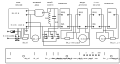
\includegraphics[width=\textwidth]{2_7_2}
	\caption{Блок-схема установки для измерения дробового шума. Внизу изображена
нижняя часть передней панели с ручками и кнопками управления}
	\figmark{exp Schottky noise}
\end{figure}

Сила анодного тока шумового диода в режиме насыщения определяется эмиссией 
(а значит, температурой) его катода. Анодный ток~$I_{\text{а}}$ измеряется 
миллиамперметром и регулируется потенциометром~$R_{\text{а}}$, ручка которого 
на панели прибора обозначена~<<$R_{\text{а}}$>>. Чувствительность измерительной 
схемы регулируется делителем напряжения~$R_{\text{д}}$, расположенным между 
усилителем и квадратичным детектором. Его ручка на панели 
обозначена~<<$R_{\text{д}}$>>. На выходе квадратичного детектора установлен
микроамперметр. Отклонение стрелки микроамперметра пропорционально квадрату
напряжения на входе детектора, поэтому он
пригоден для измерения переменных напряжений. Таким образом, показания
микроамперметра пропорциональны квадрату шумового
напряжения, причём коэффициент пропорциональности зависит от положения реостата
$R_{\text{д}}$ и, вообще говоря, неизвестен.
Поэтому при измерениях экспериментатор замечает показание микроамперметра, а
затем вместо сигнала с колебательного
контура подаёт на вход усилителя калибровочный сигнал с настроенного на ту же
частоту генератора. Этот сигнал измеряется
вольтметром (обозначение <<$U_{\text{г}}$>> на панели) и ослабляется в точно
известное число раз прецизионным аттенюатором. При
измерениях напряжение на генераторе подбирается так, чтобы стрелка
микроамперметра вернулась к отмеченному делению. В
этом случае напряжение шумов равно известному напряжению, подаваемому на
усилитель с аттенюатора. Делитель $R_{\text{д}}$ во
время этой процедуры, конечно, нельзя трогать.

Генератор используется не только для калибровки квадратичного детектора, но и
для измерения добротности контура.
Измерения производятся по методу $Q$-метра. Включим в контур генератор~Г
(настроенный на собственную частоту контура),
как это изображено на рис.~\figref{scheme Q}. Выходное напряжение генератора
$U_{\text{г}}$ целиком падает на активном сопротивлении контура $R$.
Поэтому $U_{\text{г}}=IR$, где $I$~--- ток в контуре. Найдём теперь напряжение
$U_{\text{к}}$, подаваемое на усилитель и измеряемое
квадратичным детектором:
\begin{equation*}
U_{\text{к}}=U_{\text{г}}-\frac{I}{i\omega
C}=U_{\text{г}}-\frac{U_{\text{г}}}{i\omega
RC}\approx\frac{iU_{\text{г}}}{\omega RC}.
\end{equation*}
При написании последнего равенства считалось, что контур обладает высокой
добротностью, $Q=1/\omega RC\gg1$. Заменяя $1/\omega
RC$ через добротность контура, найдём
\begin{equation}
	\eqmark{2.7.13}
	Q=\frac{|U_{\text{к}}|}{|U_{\text{г}}|}.
\end{equation}

\begin{figure}[h!]
    \centering\small
	\pic{0.6\textwidth}{Chapter_2/2_7_3}
	%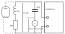
\includegraphics[width=\textwidth]{2_7_3}
	\caption{Схема для измерения добротности колебательного контура}
	\figmark{scheme Q}
\end{figure}

Итак, для измерения добротности контура нужно сравнить напряжение на генераторе
с напряжением на катушке самоиндукции.
Напряжение на генераторе $U_{\text{г}}$ измеряется вольтметром генератора
(рис.~\figref{exp Schottky noise}). Измерение напряжения на катушке самоиндукции
не так просто.

При измерении напряжения $U_{\text{к}}$, создаваемого генератором на катушке
самоиндукции, необходимо учитывать и шумовое
напряжение $U_{\text{ш}}$, имеющееся на катушке. Это напряжение при измерениях
продолжает возбуждаться диодом, так как при
измерениях добротности контура диод находится в рабочем режиме. Отключить диод
при измерении нельзя, поскольку
добротность контура от этого заметно изменится: при измерениях шума контур
шунтирован диодом, что снижает его
добротность; в этом положении и должна измеряться добротность контура. При
включении генератора в контур на вход
усилителя поступает не $U_{\text{к}}$, как показано на рис.~\figref{scheme Q}, и
не $U_{\text{ш}}$, а их сумма. При этом ток детектора $I_{\text{д}}$
пропорционален
$\langle (U_{\text{ш}}+U_{\text{к}})^2\rangle$. Сдвиг фаз между колебаниями
$U_{\text{ш}}$ и $U_{\text{к}}$ непрерывно изменяется. Поэтому
\begin{equation*}
I_{\text{д}}\propto\langle (U_{\text{ш}}+U_{\text{к}})^2\rangle=\langle
U_{\text{ш}}^2\rangle+2\langle U_{\text{ш}}U_{\text{к}}\rangle+\langle
U_{\text{к}}^2\rangle=\langle U_{\text{ш}}^2\rangle+\langle
U_{\text{к}}^2\rangle,
\end{equation*}
в то время как до включения генератора ток детектора $I_{\text{д}}$ был
пропорционален $U_{\text{ш}}^2$.

Таким образом, $U_{\text{к}}^2$ пропорционально \important{приращению} тока
квадратичного детектора, происходящему при включении
напряжения $U_{\text{г}}$. Чтобы подставить это приращение в формулу
\eqref{2.7.13}, оно должно быть пересчитано в напряжение
генератора. Это делается следующим образом. Нужно заметить показание
квадратичного детектора при нулевом напряжении на
выходе генератора. Затем нужно установить на выходе генератора некоторое
напряжение $U_{\text{г}}$ и зафиксировать приращение
тока детектора $\Delta I_{\text{д}}$, вызванное напряжением генератора. После
этого вместо колебательного контура на вход усилителя
следует подключить генератор с аттенюатором. Сигнал с генератора и положение
аттенюатора нужно подобрать таким образом,
чтобы показание микроамперметра было равно измеренному ранее приращению $\Delta
I_{\text{д}}$. Показание вольтметра генератора равно
искомому напряжению $U_{\text{к}}$.

%\todo[author=Tiffani]{Сделать нормальный рисунок. Этот даже не отображается}
\begin{figure}[h!]
    \centering\small
	\pic{0.85\textwidth}{Chapter_2/2_7_4}
	\caption{Схема установки для измерения напряжения шума}
	\figmark{scheme U noise}
\end{figure}

\begin{lab:task}
\taskpreamble{В работе предлагается, измерив напряжение шумов, раскачивающих колебательный
контур, и определив добротность этого
контура, рассчитать заряд электрона.}

\tasksection{Проверка квадратичности детектора}

	\item Включите питание стенда (кнопка <<Сеть>>).

	\item Убедитесь в том, что выпрямительная схема с полупроводниковыми диодами
действительно имеет квадратичную
характеристику. Для этого включите стенд в режим измерения напряжения генератора
(кнопка <<$U_{\text{г}}$>>). Установите
максимальную  чувствительность квадратичного детектора
(регулятор~$R_{\text{д}}$) и подберите предел измерений для вольтметра
(кнопка <<100>> или <<300>>~мкВ аттенюатора). Изменяя выходное напряжение
генератора с помощью регулятора напряжения генератора~$R_{г}$, 
измерьте зависимость тока квадратичного детектора~$I_{\text{д}}$ 
от входного напряжения усилителя~$U_{\text{г}}$.

\tasksection{Измерение напряжения шума}

	\item Включите режим измерения шума (кнопка <<$U_{ш}$>>).
Электрическая схема для этого случая показана на рис.~\figref{scheme U noise}.

	\item Установите анодный ток шумового диода $I_{а}=1$~мА, изменяя
регулятором $R_{А}$ напряжение накала диода.

С помощью регулятора $R_{д}$ подберите чувствительность квадратичного
детектора так, чтобы стрелка микроамперметра
отклонялась на б\'{о}льшую часть шкалы. Отметьте значение шумового
тока~$I_{д}$.

Для пересчёта отклика детектора на шум в единицы напряжения вместо шумового
диода подключите к усилителю генератор напряжений (кнопка~<<$U_{г}$>>).
Измерительная схема приведена на рис.~\figref{scheme U generator}.

С помощью регулятора $R_{г}$ и аттенюатора (пределы <<30>>, <<100>> или
<<300>>~мкВ) установите \important{то же значение тока} $I_{д}$,
которое было выбрано в режиме измерения шума. Регулятор~$R_{д}$ во время
этой процедуры, конечно, трогать нельзя. Отсчитанное по вольтметру
с аттенюатором напряжение~$U_{эфф}$ равно корню квадратному из среднего
квадрата напряжения шумов.

\begin{figure}[h!]
    \centering\small
    \pic{0.8\textwidth}{Chapter_2/2_7_5}
    \caption{Схема установки для измерения напряжения на генераторе}
    \figmark{scheme U generator}
\end{figure}

\tasksection{Измерение добротности контура}

	\item При том же анодном токе диода переключите аттенюатор в положение <<1>>
или <<3>>~мкВ. Установите режим измерения
напряжения на контуре при его последовательном возбуждении
(кнопка~<<$U_{\text{к}}$>>). При нулевом напряжении на вольтметре
подберите чувствительность детектора: регулятором $R_{\text{д}}$ установите
стрелку микроамперметра детектора на любое целое
деление. Измерьте \important{приращение} тока детектора $\Delta I_{\text{д}}$
при изменении напряжения генератора от нуля до любого
напряжения~$V_1$.

Затем включите режим измерения напряжения на генераторе
(кнопка~<<$U_{\text{г}}$>>) и регулятором $R_{\text{г}}$ подберите напряжение
$V_2$, при котором ток квадратичного детектора равен \important{приращению}
$\Delta I_{\text{д}}$ в режиме измерения сигнала с~контура.
Добротность контура равна $Q=V_2/V_1$.

	\item Повторите измерения п.~2--3 ещё 5--6 раз при том же
анодном токе (можно при другой чувствительности детектора).

	\item Проведите измерения п.~2--4 при других значениях анодного
тока в интервале 1--4~мА.

	\item Запишите значения ёмкости и резонансной частоты колебательного
контура, указанные на установке.

\tasksection{Обработка результатов}

	\item Постройте график зависимости $I_{\text{д}}=f(U^2_{\text{г}})$ для
проверки характера детектирования.

	\item Вычислите среднюю величину заряда электрона для каждого значения тока
анода. Представьте результаты в виде таблицы.

%\bigskip
\begin{center}
\begin{tabular}{|c|c|c|c|c|}
\hline $\;I_{\text{а}}$,~мА&$\;U_{\text{эфф}}$,~мкВ&$\quad\langle
Q\rangle\quad$&$e~$, Кл&$\langle e\rangle\pm\Delta e$\\\hline
 & & & &\\
 & & & &\\
\hline
\end{tabular}
\end{center}

	\item Определите заряд электрона, используя все полученные результаты, и
оцените погрешность. Сравните полученное значение
с табличным.
\end{lab:task}

%\todo[author=Tiffani]{Нет вопросов к лабораторной.}

\begin{lab:literature}
    \item \Kirichenko~--- \S 18.1.
	\item *\textit{Власов~В.Ф.} Электронные и ионные приборы.~--- М.:~Связьиздат,
1960, \S 13.5.
	\item *\textit{Рытов~С.М.} Введение в статистическую радиофизику.~---
М.:~Наука, 1976, \S 5.
\end{lab:literature}

\lab{Релаксационные колебания}

\aim{изучение вольт-амперной характеристики нормального тлеющего разряда;
исследование релаксационного генератора на стабилитроне.}

\equip{стабилитрон СГ-2 (газонаполненный диод) на монтажной панели, амперметр,
вольтметр, магазин сопротивлений, магазин ёмкостей, источник питания,
осциллограф (ЭО), генератор звуковой частоты (ЗГ).}

Колебательные системы, как правило, имеют два накопителя энергии, между
которыми происходит её перекачка. В контуре,
содержащем конденсатор и катушку индуктивности, электрическая энергия переходит
в магнитную и обратно.

\begin{figure}[h!]
	\pic{0.9\textwidth}{Chapter_2/5_1_1}
	\caption{Вольт-амперная характеристика стабилитрона с последовательно
включённым резистором}
	\figmark{VACH stabilitron}
\end{figure}
%\rpic{38mm}{5_1_1}{\cct Вольт-амперная характеристика стабилитрона с
%последовательно включённым резистором}{1}

Встречаются, однако, колебательные системы, содержащие всего один накопитель
энергии. Рассмотрим в качестве примера
электрическую цепь, содержащую конденсатор и сопротивление без самоиндукции.
Разряд конденсатора через сопротивление
представляет собой апериодический процесс. Разряду, однако, можно придать
периодический характер, возобновляя заряд
конденсатора через постоянные промежутки времени. Колебания в этом случае
являются совокупностью двух апериодических
процессов~--- процесса зарядки конденсатора и процесса его разрядки. Такие
колебания называются релаксационными.

В нашей установке роль <<ключа>>, обеспечивающего попеременную зарядку и
разрядку конденсатора, играет газоразрядный
диод. Зависимость тока от напряжения для газоразрядной лампы не подчиняется
закону Ома и характеризуется рядом
особенностей (рис.~\figref{VACH stabilitron}). При малых напряжениях лампа
практически не пропускает тока (см. участок ОАБ на рис.~$v5_r2 и v5_r6$).
\todo[author=Tiffani]{Ссылки на непонятные}
Ток в лампе возникает только в том случае, если разность потенциалов на её
электродах достигает \important{напряжения зажигания} $V_1$. 
При этом скачком устанавливается конечная сила тока $I_1$~---~в лампе возникает
\important{нормальный тлеющий разряд}. При дальнейшем незначительном увеличении
напряжения сила тока заметно возрастает по закону, близкому к линейному. 
Нормальный тлеющий разряд~---~стабилизатор напряжения, отсюда второе название 
лампы~---~\important{стабиловольт}.


\begin{figure}[h!]
	\pic{0.9\textwidth}{Chapter_2/5_1_2}
	\caption{Принципиальная схема релаксационного генератора}
	\figmark{generator scheme}
\end{figure}
%\rpic{4.0cm}{5_1_2}{\cct Принципиальная схема релаксационного генератора}{2}


Если начать уменьшать напряжение на горящей лампе, то при напряжении, равном
$V_1$, лампа ещё не гаснет, и сила тока
продолжает уменьшаться. Лампа перестанет пропускать ток лишь при
\important{напряжении гашения}~$V_2$, которое обычно
существенно меньше $V_1$. Сила тока при этом скачком падает от значения~$I_2$
($I_2<I_1$) до нуля.

Характеристика, изображённая на рис.~\figref{VACH stabilitron}, несколько
идеализирована. У~реальной лампы зависимость $I(V)$ не вполне линейна.
При $V>V_1$ графики, соответствующие возрастанию и убыванию напряжения, не
всегда совпадают. Эти отличия, впрочем, носят
второстепенный характер и для нашей задачи несущественны.

\begin{figure}[h!]
	\pic{0.9\textwidth}{Chapter_2/5_1_3}
	\caption{Режимы работы релаксационного генератора}
	\figmark{generator work}
\end{figure}
%\rpic[14]{4.0cm}{5_1_3}{\cct Режимы работы релаксационного генератора}{3}

Рассмотрим схему релаксационного генератора, представленную
на\\*рис.~\figref{generator scheme}. Пусть напряжение батареи $U$ больше
напряжения
зажигания $V_1$. В обозначениях, принятых на схеме, справедливо уравнение
\begin{equation*}
I_C+I(V)=\frac{U-V}{R}
\end{equation*}
или
\begin{equation}
	\eqmark{2.8.1}
	C\frac{dV}{dt}+I(V)=\frac{U-V}{R}.
\end{equation}
В стационарном режиме работы, когда напряжение $V$ на конденсаторе постоянно и
$dV/dt = 0$, ток через лампу равен
\begin{equation}
	\eqmark{2.8.2}
	I_{\text{ст}}=\frac{U-V}{R}.
\end{equation}

Равенство \eqref{2.8.2} может быть представлено графически
(рис.~\figref{generator work}).
При разных $R$ графики имеют вид прямых, пересекающихся в точке $V=U$,\\*$I=0$.
Область, где эти \important{нагрузочные прямые}
пересекают вольт-амперную характеристику лампы, соответствует стационарному
режиму~---~при малых $R$ (прямая~1) лампа
горит постоянно, колебания отсутствуют. Прямая~2, проходящая через точку
($I_2$,~$V_2$), соответствует критическому
сопротивлению
\begin{equation}
	\eqmark{2.8.3}
	R_{\text{кр}}= \frac{U-V_2}{I_2}.
\end{equation}
При сопротивлении $R>R_{\text{кр}}$ нагрузочная прямая~3 не пересекает
характеристику лампы, поэтому стационарный режим
невозможен. В этом случае в системе устанавливаются колебания.

Рассмотрим, как происходит колебательный процесс. Пусть в начале опыта ключ~К
разомкнут (рис.~\figref{generator scheme}) и $V=0$. Замкнём ключ.
Конденсатор~$C$ начинает заряжаться через сопротивление~$R$, напряжение на нём
увеличивается (рис.~\figref{relax osc}). Как только оно
достигнет напряжения зажигания $V_1$, лампа начинает проводить ток, причём
прохождение тока сопровождается разрядкой
конденсатора. В самом деле, батарея~$U$, подключённая через большое
сопротивление~$R$, не может поддерживать необходимую
для горения лампы величину тока. Во время горения лампы конденсатор разряжается,
и когда напряжение на нём достигнет
потенциала гашения, лампа перестанет проводить ток, а конденсатор вновь начнёт
заряжаться. Возникают релаксационные
колебания с~амплитудой, равной $(V_1-V_2)$.

\begin{figure}[h!]
	\pic{0.9\textwidth}{Chapter_2/5_1_4}
	\caption{Осциллограмма релаксационных колебаний}
	\figmark{relax osc}
\end{figure}
%\rpic{5.0cm}{5_1_4}{\cct Осциллограмма релаксационных колебаний}{4}

Рассчитаем период колебаний. Полное время одного периода колебаний $T$ состоит
из суммы времени зарядки $\tau_{\text{з}}$ и
времени разрядки $\tau_{\text{р}}$, но если сопротивление $R$ существенно
превосходит сопротивление зажжённой лампы, то
$\tau_{\text{з}}\gg \tau_{\text{р}}$ и $T\approx\tau_{\text{з}}$ (этим случаем
мы и ограничимся).

Во время зарядки конденсатора лампа не горит ($I(V)=0$), и уравнение
\eqref{2.8.1} приобретает вид
\begin{equation}
	\eqmark{2.8.4}
	RC\frac{dV}{dt}=U-V.
\end{equation}
Будем отсчитывать время с момента гашения лампы, так что $V=V_2$ при $t=0$
(рис.~\figref{relax osc}). Решив уравнение \eqref{2.8.4}, найдём
\begin{equation}
	\eqmark{2.8.5}
	V=U-(U-V_2)e^{-t/RC}.
\end{equation}
В момент зажигания $t=\tau_{\text{з}}$, $V=V_1$, поэтому
\begin{equation}
	\eqmark{2.8.6}
	V_1=U-(U-V_2)e^{-\tau_{\text{з}}/RC}.
\end{equation}
Из уравнений \eqref{2.8.5} и \eqref{2.8.6} нетрудно найти период колебаний:
\begin{equation}
	\eqmark{2.8.7}
	T\approx \tau_{\text{з}}=RC\ln\frac{U-V_2}{U-V_1}.
\end{equation}

Развитая выше теория является приближённой. Ряд принятых при расчётах упрощающих
предположений оговорен в тексте.
Следует иметь в виду, что мы полностью пренебрегли паразитными емкостями и
индуктивностями схемы. Не рассматривались
также процессы развития разряда и деионизация при гашении. Поэтому теория
справедлива лишь в~тех случаях, когда в схеме
установлена достаточно большая ёмкость и когда период колебаний существенно
больше времени развития разряда и времени
деионизации (практически $\gg10^{-5}$~с). Кроме того, потенциал гашения $V_2$,
взятый из статической вольт-амперной
характеристики, может отличаться от потенциала гашения лампы, работающей в
динамическом режиме релаксационных колебаний.

\begin{lab:task}

\taskpreamble{В работе предлагается снять вольт-амперную характеристику
стабилитрона и познакомиться с работой релаксационного генератора: определить
критическое сопротивление, исследовать зависимость периода колебаний от
сопротивления при фиксированной ёмкости и от ёмкости при фиксированном
сопротивлении.}

\tasksection{Характеристика стабилитрона}
\begin{figure}[h!]
	\pic{0.9\textwidth}{Chapter_2/5_1_5} % закоммент. т.к. не работает
	\caption{Схема установки для~изучения характеристик стабилитрона}
	\figmark{stabilitron scheme charact}
\end{figure}
%\rpic{5.0cm}{5_1_5}{\cct Схема установки для~изучения характеристик
%стабилитрона}{5}

		\item Соберите схему, изображённую на рис.~\figref{stabilitron scheme
charact}. Добавочное сопротивление $r$ подпаяно между ножкой лампы и
соответствующей
клеммой для того, чтобы предохранить стабилитрон от перегорания. Это
сопротивление остаётся включённым при всех
измерениях. Запишите величину $r$, указанную на панели лампы.

		\item Установите регулятор источника питания на минимум напряжения и
включите источник в сеть.

		\item Снимите вольт-амперную характеристику стабилитрона с
сопротивлением $r$ при возрастании и убывании напряжения. При
этом как можно точнее определите потенциалы зажигания и гашения $V_1$ и $V_2$ и
соответствующие токи $I_1$ и $I_2$.

\tasksection{Осциллограммы релаксационных колебаний}

		\item Соберите релаксационный генератор согласно
         рис.~\figref{scheme exp osc}.

		\item Установите на магазине ёмкостей значение $C=0,05$~мкФ, а на
магазине сопротивлений $R=900$~кОм.

		\item Включите в сеть осциллограф, звуковой генератор и источник питания
и установите напряжение $U\approx 1,2\,V_1$.

\begin{figure}[h!]
	\pic{0.9\textwidth}{Chapter_2/5_1_6}
	\caption{Схема установки для исследования релаксационных колебаний}
	\figmark{scheme exp osc}
\end{figure}
%\fcpic[1]{5_1_6}{Схема установки для исследования релаксационных колебаний}{6}

		\item Подберите частоту развёртки ЭО, при которой на экране видна
картина пилообразных колебаний (рис.~\figref{relax osc}).

		\item Получив пилу на экране, оцените соотношение между временем
зарядки~$\tau_{\text{з}}$ и временем разрядки $\tau_{\text{р}}$.
Зарисуйте картину колебаний.

		\item Уменьшая сопротивление магазина, определите $R_{\text{кр}}$, при
котором пропадают колебания, и сравните его с величиной,
рассчитанной по формуле~\eqref{2.8.3}. Это сравнение полезно сделать в процессе
работы и подумать о причинах расхождения
результатов.

Убедитесь, что колебания пропадают не только при уменьшении $R$ при постоянном
$U$, но и при увеличении $U$ при
постоянном $R$, когда это $R$ не слишком превышает $R_{\text{кр}}$.

\tasksection{Фигуры Лиссажу и частота колебаний}

		\item Восстановите исходные параметры релаксационного
генератора:\\*$C=5\cdot 10^{-2}$~мкФ, $R=900$~кОм, $U\approx 1,2 \cdot
V_1$. Подайте сигнал с генератора на вход $X$ осциллографа. Меняя частоту ЗГ,
получите на экране фигуру Лиссажу без
самопересечений, соответствующую отношению частот 1:1.

		\item Не меняя параметров релаксационного генератора, уменьшите частоту
ЗГ вдвое (втрое) и получите фигуры Лиссажу при
соотношении частот 2:1 (3:1). Зарисуйте эти кривые в тетрадь.

Получите и зарисуйте фигуры Лиссажу при увеличении частоты ЗГ в два и три раза
(1:2 и 1:3).

		\item При любом целом значении $R$ из интервала (2~--~4)~$R_{\text{кр}}$
снимите с помощью фигур Лиссажу 1:1 зависимость частоты
колебаний $\nu$ от ёмкости~$C$, меняя величину ёмкости в пределах от
$5\cdot10^{-2}$ до $5\cdot10^{-3}$~мкФ.

Напряжение $U$, необходимое для расчёта теоретического значения периода по
формуле \eqref{2.8.7}, следует поддерживать
постоянным.

		\item Проведите серию измерений $\nu=f(R)$ при постоянной ёмкости\\*
$C=5\cdot10^{-2}$, меняя величину $R$ от максимального
значения до критического.

\tasksection{Обработка результатов}

		\item Постройте графики $I=f(V)$ для системы, состоящей из стабилитрона
и дополнительного сопротивления $r$ (по результатам
измерений) и для стабилитрона без сопротивления~$r$ (вычитая падение напряжения
на сопротивлении~$r$ при каждом токе).
Сравните относительные изменения тока и напряжения на стабилитроне.

		\item Рассчитав экспериментальные и теоретические значения периодов,
постройте графики $T_{\text{эксп}}=f(C)$ и $T_{\text{теор}}=f(C)$ на
одном листе.
На другом листе постройте графики $T_{\text{эксп}}$ и $T_{\text{теор}}=f(R)$.

		\item Если наклоны теоретической и экспериментальной прямых заметно
отличаются, рассчитайте из экспериментальной прямой
динамический потенциал гашения. Потенциалы зажигания можно считать одинаковыми.
\end{lab:task}


\begin{lab:questions}
	\item Какие колебания называются релаксационными?

	\item От каких параметров газа зависит напряжение зажигания стабиловольта?

	\item Почему напряжение гашения существенно меньше напряжения зажигания?

%	\item Какие режимы работы релаксационного генератора Вы знаете?

	\item Как по вольт-амперной характеристике стабиловольта и известным
параметрам генератора найти ток в лампе в стационарном
режиме?

	\item Что такое критическое сопротивление релаксационного генератора? От
чего оно зависит?

	\item Почему критическое сопротивление зависит от величины напряжения $U$ на
входе генератора? Рассмотрите рис.~\figref{generator work}.

	\item Почему при малой ёмкости колебания не возникают (лампа не гаснет) даже
при $R>R_{\text{кр}}$? Оцените <<малость>> ёмкости,
сравнив время релаксации и время деионизации.
\end{lab:questions}


\begin{lab:literature}

	\item \SivuhinIII~--- \S~134.

	\item \emph{Калашников~С.Г.} Электричество.~--- М.:~Наука, 1974. \S~244.

	\item \emph{Горелик~Г.С.} Колебания и волны.~--- М.:~Физматгиз, 1959.
Гл.~IV, \S~6.
\end{lab:literature}

% \lab{Электромагнитные волны в волноводе} 

\begin{lab:aim} ознакомление с особенностями распространения
    электромагнитных волн в волноводе, аппаратурой и методами измерения основных
    характеристик протекающих при этом процессов. 
\end{lab:aim}

\begin{lab:equipment} генератор сигналов сверхвысокой частоты, измерительная
    линия, усилитель, заглушка, отрезок волновода с поглощающей нагрузкой, отрезки
    волноводов различных сечений, детекторная головка. 
\end{lab:equipment}

Передача энергии электромагнитных колебаний низкой частоты, например, 50~Гц, не
представляет проблем и делается широко известным способом: по проводам. На более
высоких частотах (до 300~МГц) эта задача решается с помощью двухпроводных линий
и коаксиальных кабелей. На ещё более высоких частотах (до 300~ГГц) при
колебаниях с длинами волн (в вакууме) от 1~метра до 1~миллиметра (этот диапазон
называется \important{диапазоном сверхвысоких частот} или, сокращённо, СВЧ)
передача энергии с помощью двухпроводной линии или коаксиальных кабелей
становится малоэффективной из-за больших потерь: резко возрастает сопротивление
проводов из-за \important{скин-эффекта}~---~вытеснения тока на поверхность, а в
двухпроводной линии, кроме того, потери растут вследствие излучения энергии в
окружающее пространство.

В СВЧ-диапазоне энергия передаётся с помощью металлических труб, называемых
волноводами (в миллиметровом диапазоне длин волн волноводы могут быть сделаны и
из диэлектрика). Электромагнитные волны могут распространяться по металлическим
трубам любого профиля, но из технологических соображений сечения волноводов
делаются либо круглыми, либо прямоугольными.

Чтобы найти структуру электромагнитного поля в волноводе, надо решить уравнения
Максвелла с соответствующими граничными условиями. Решение этой задачи приведено
во многих учебниках.

Для радиоволн, бегущих по волноводу вдоль оси $Z$ с проводящими стенками,
расположенными на расстоянии $a$ друг от друга (простейший волновод), с вектором
напряженности электрического поля $\vec E=E_y \vec e_y,$ перпендикулярным
плоскости $ZX$. Такое решение может быть записано в виде: 
\begin{equation}
\eqmark{2.0.1} E_y=A\sin\left(\dfrac{n\pi x}{a}\right)\sin(\omega t-k_zz),
\qquad n=0,~1,~2,~3 \ldots, 
\end{equation} 
где $k_z=\sqrt{k^2-k^2_x},
k=2\pi/\lambda_0=\omega/c, \lambda_0$~---~длина волны в вакууме, $\omega=2\pi
f$, $f$~---~частота генератора, $c$~---~скорость света. Множитель
$\sin\left(\dfrac{n\pi x}{a}\right)$ физически соответствует стоячей волне между
стенками волновода по координате $Х$ и определяет граничные условия $E_y=0$ на
проводящих стенках.

\begin{figure}[h!]
    %\centering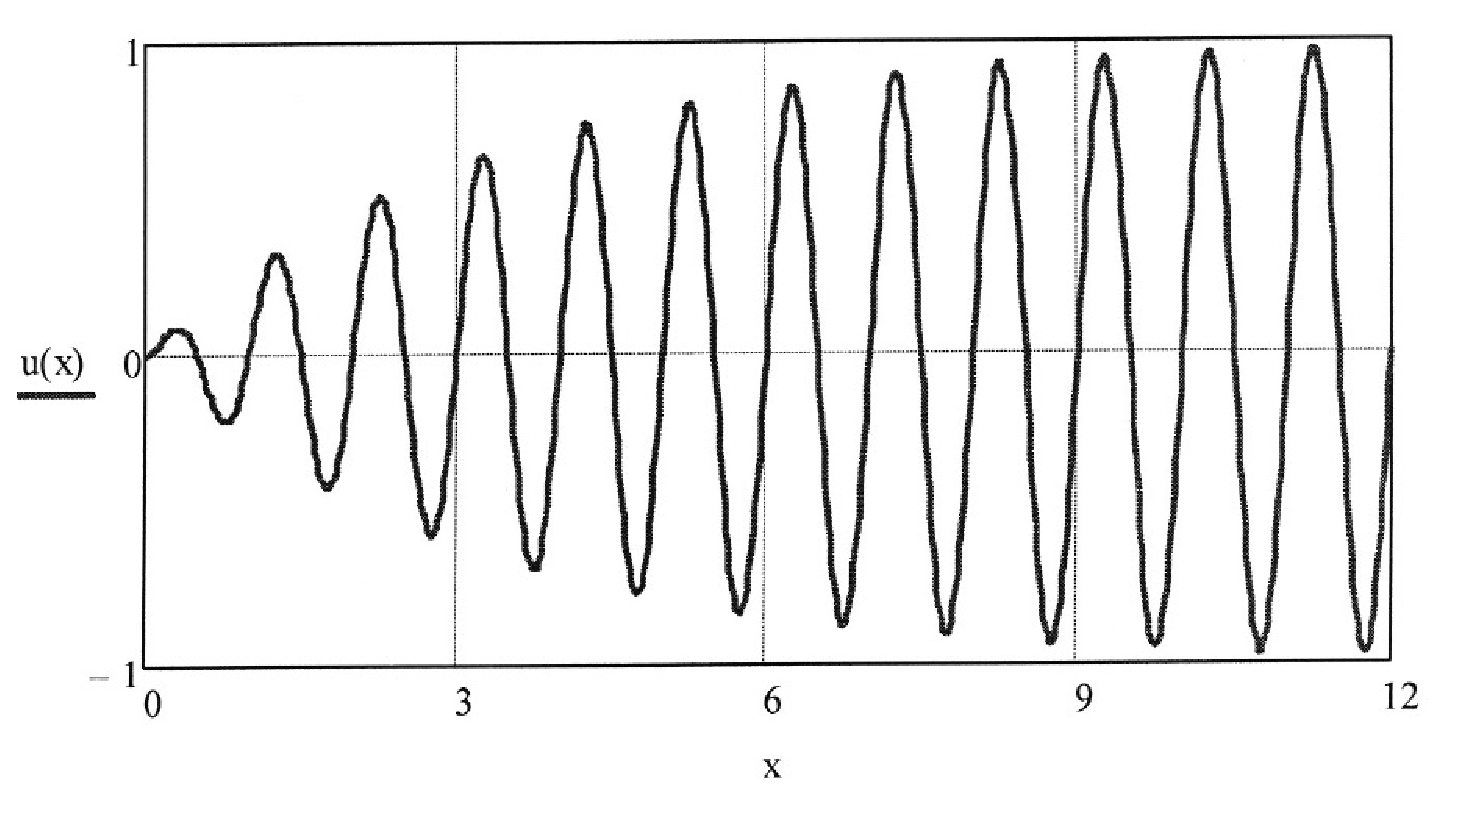
\includegraphics[width=0.6\linewidth]{Chapter_2/13}
    \caption{Волновод и примеры распределения поля} \figmark{waveguide}
\end{figure}

Для бегущих вдоль волновода волн $k_z$~---~действительная величина. Предельный
случай $k_z=0$ соответствует $k=k_x,$ что при условии $n=1$ приводит к формулам
для \important{критических длины и циклической частоты волн}, распространяющихся
в вакуумном волноводе: 
\begin{equation} 
\eqmark{2.0.2} \lambda_{\text{кр}}=2a,
\qquad \omega_{\text{кр}}=\pi c/a. 
\end{equation} 
Если $\lambda>2a$ и,
соответственно, $\omega<\pi c/a,$ то электромагнитная волна при распространении
вдоль волновода затухает.

Для бегущей волны фазовая скорость \begin{equation} \eqmark{2.0.3}
V_{\text{Ф}}=\omega/k_z=c/\sqrt{1-\omega^2_{\text{кр}}/\omega^2} \end{equation}
больше скорости света в вакууме $c,$ а длина волны в волноводе \begin{equation}
\eqmark{2.0.4} \lambda_{\text{В}}=\lambda_0/\sqrt{1-(\lambda_0/2a)^2}
\end{equation} больше длины волны в вакууме $\lambda_0.$ В представленном на
рис.~\figref{waveguide} случае отлична от нуля продольная составляющая
магнитного поля, и такую волну называют \important{магнитной ($H$-волна).}
Обычно для передачи СВЧ-энергии по прямоугольному волноводу используется волна
(мода) $H_{10}.$  Второй индекс $0$ соответствует отсутствию составляющей
электромагнитного поля $E_x.$ Критическая длина волны моды
$H_{10}$~---~максимальная среди всех типов волн в прямоугольном волноводе, и
поэтому ее называют \important{основной.} Тем самым, для волновода заданного
сечения существует диапазон частот, ограниченный снизу критической частотой
волны $H_{10}$ ($\lambda_{\text{кр}}=2a$). Следующая по возрастанию
частоты~---~мода $H_{01}$ с $\lambda_{\text{кр}}=2b$ или $H_{20}$ с
$\lambda_{\text{кр}}=a,$ если $a>b.$

В заданном частотном диапазоне СВЧ-энергия может переноситься одним типом волн,
что существенно облегчает её дальнейшее использование.

Если в волноводе имеется какое-либо препятствие, нерегулярность, то в нём
появляется \important{отражённая волна.} Падающая $E_0$ и отраженная волна с
коэффициентом отражения $\rho$ по амплитуде интерферируют и создают в волноводе
стоячую волну.

Максимальное (в пучности) и минимальное (в узле) значения поля равны
соответственно 
\begin{equation} \eqmark{2.0.5} 
E_{\text{max}}=E_0(1+\rho),
\qquad E_{\text{min}}=E_0(1-\rho). 
\end{equation} 
Отношение
$K=E_{\text{max}}/E_{\text{min}}$ называется \important{коэффициентом стоячей
    волны} (к.с.в.). Коэффициент отражения от препятствия по амплитуде
\begin{equation} \eqmark{2.0.6}
\rho=\dfrac{E_{\text{max}}-E_{\text{min}}}{E_{\text{max}}+E_{\text{min}}}=\dfrac{K-1}{K+1}. 
\end{equation}

В случае полного отражения (металлическая заглушка) $\rho=1,$ а если в волновод
вставлено вещество, поглощающее СВЧ-­излучение (согласованная нагрузка), то
$\rho=0.$

Для определения коэффициента стоячей волны обычно используют измерительную
линию~---~отрезок волновода с продольной щелью длиной в несколько полуволн. В
щели располагается зонд~---~большой металлический штырь (антенна), реагирующий
на электрическое поле в волноводе. Напряжение высокой частоты, наводимое на
зонд, детектируется, усиливается и подаётся на микровольтметр. Зонд может
перемещаться вдоль линии, что позволяет исследовать распределение электрического
поля в волноводе.

\labsection{А. Волны в волноводе при частоте выше критической}

\experiment Схема для исследования структуры волн в волноводе при частоте выше
критической представлена на рис.~\figref{scheme microwave}. Модулированный
сигнал от высокочастотного генератора (цуги с частотой повторения 1~кГц)
поступает на вход измерительной линии, вдоль которой перемешается зонд~8.
Высокочастотный сигнал с зонда поступает на кристаллический детектор $D$.

\begin{figure}[h!]
    %\centering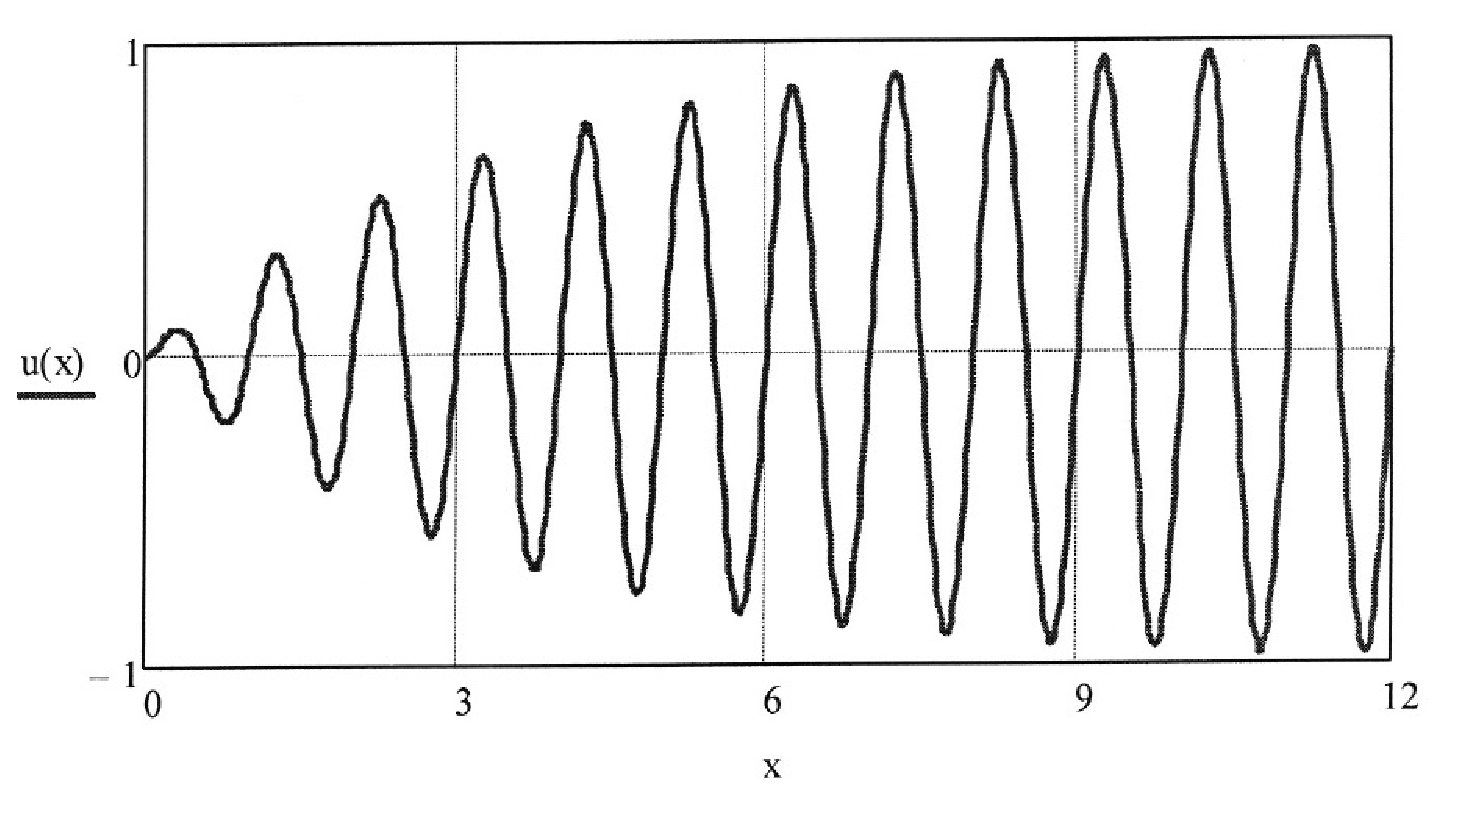
\includegraphics[width=0.6\linewidth]{Chapter_2/13}
    \caption{Схема для исследования структуры волн СВЧ} \figmark{scheme microwave}
\end{figure}

С нагрузки детектора (с $RС$-цепочки) снимается огибающая высокочастотного
сигнала и подаётся на усилитель низкой частоты. Величина сигнала регистрируется
вольтметром, вмонтированным в усилитель. Ручка~$С$~---~настройка измерительной
линии~--- служит для согласования зонда (как антенны) со входом усилителя. Как
правило, они согласованы, и в настройке нет необходимости. В волноводе с
закрытым выходом образуется стоячая волна. Определив расстояние между узлами,
можно рассчитать длину волны и фазовую скорость СВЧ-сигнала в волноводе.
Устройство детекторной головки, установленной на измерительной линии, таково,
что отклик вольтметра $U$ на величину напряжённости электрического поля $Е$ в
волноводе \begin{equation*} U\sim E^{n}, \end{equation*} а показатель степени
$n$ сам зависит от величины сигнала: при малых сигналах детектирование
квадратичное $(n=2),$ при больших~---~линейное $(n=1).$

Меняя нагрузку на выходе измерительной линии (ручка~$B$ на рис.~\figref{scheme
    microwave}) и сравнивая максимальное и минимальное показания вольтметра, можно
рассчитать коэффициент стоячей волны $K$ и коэффициент отражения $\rho.$

\labsection{Б. Волны в волноводе при частоте ниже критической}

Для исследования затухания волн в волноводе при частоте ниже критической
используются те же генератор, усилитель, измерительная линия и дополнительный
набор волноводов с отдельной детекторной головкой $G$ (рис.~\figref{scheme
    damping}). Дополнительный набор начинается и заканчивается волноводами
переменного сечения I и II. Между ними

\begin{figure}[h!]
    %\centering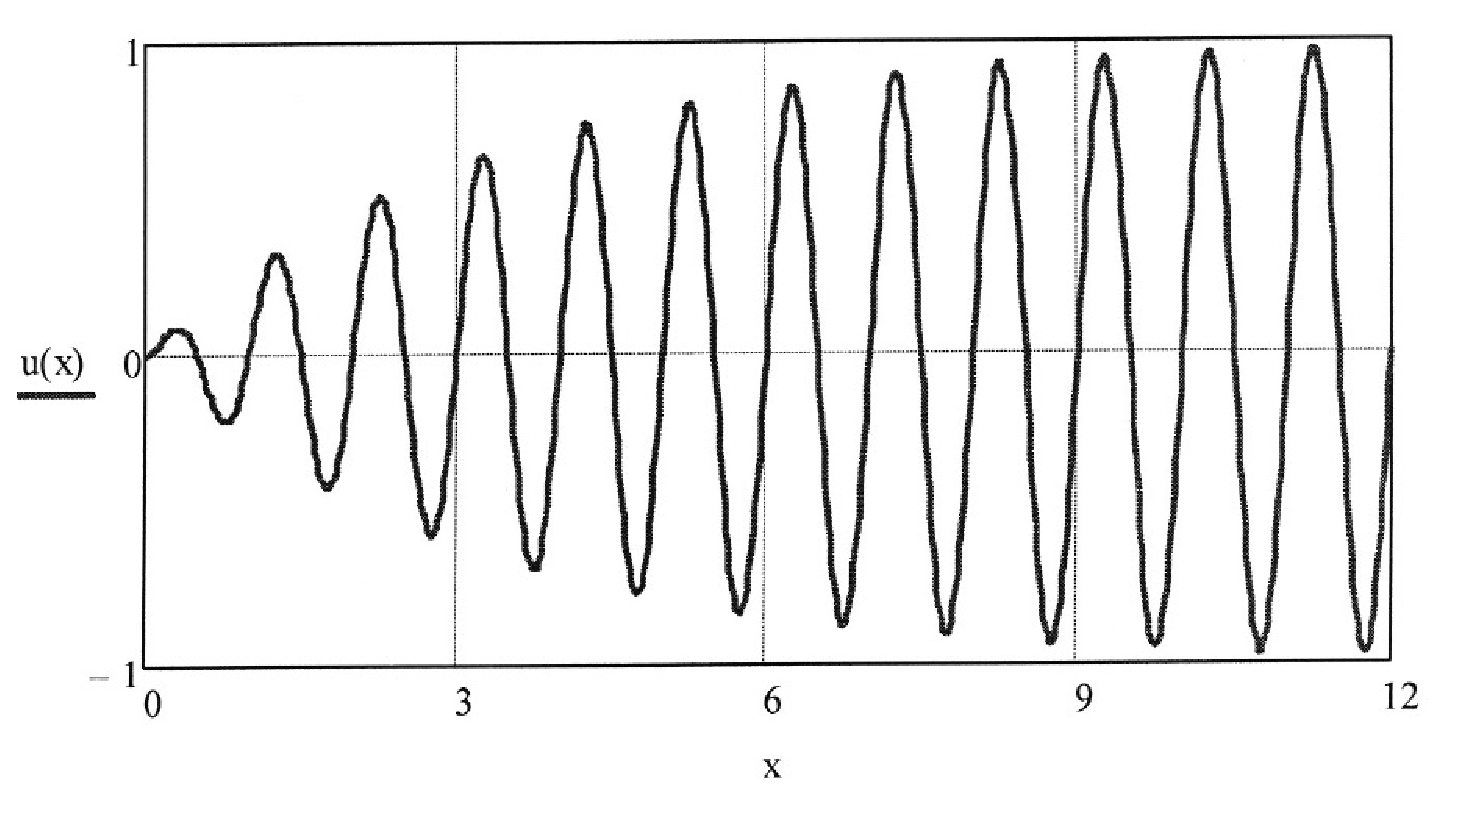
\includegraphics[width=0.6\linewidth]{Chapter_2/13}
    \caption{Схема для исследования затухания} \figmark{scheme damping}
\end{figure}

можно разместить 1,~2 или 3 одинаковых отрезка с постоянным сечением. В такой
системе волны с частотами меньше критической экспоненциально затухают.

Мощность сигнала на выходе из волновода $W$ можно связать с мощностью входного
сигнала $W_0$ двумя способами: $W=W_0e^{-\alpha z}$ или $W=W_0~10^{-\beta z},$
где $z$~---~длина волновода. Величина $(\alpha z)$ измеряется в Неперах (Нп):
один Непер соответствует отношению интенсивностей, равному основанию натуральных
логарифмов. Величину $(\beta z)$ принято измерять в децибелах (дБ): один Бел
соответствует уменьшению мощности в 10 раз; децибел~---~одна десятая Бела.
Измеренное в децибелах затухание определяется формулой $\beta
z(\text{дБ})=10\times\lg(W_0/W).$ Отсюда следует, что
$\alpha(\text{Нп})=2,3\beta(\text{Б}).$

Если при уменьшении количества вставок волновода поддерживать интенсивность
выходного сигнала постоянной, то входной сигнал следует ослабить. Степень
ослабления $\gamma$ зависит от длины волновода $z~(\gamma~=~\beta~z)$ и
измеряется по шкале генератора в децибелах. Именно таким образом в эксперименте
определяется коэффициент затухания $\beta.$ Его можно сравнить с коэффициентом
$\alpha,$ рассчитанным теоретически. В закритическом волноводе при квадратичном
детектировании интенсивность сигнала падает по закону $E^2\sim e^{-\alpha z},$
где $\alpha$~---~коэффициент затухания: 
\begin{equation} \eqmark{2.0.7}
\alpha=2ik_{Z}=\dfrac{2\omega}{c}\sqrt{\left(\dfrac{\omega_{kp}}{\omega}\right)^2-1}=
\dfrac{2\pi}{a}\sqrt{1-\left(\dfrac{2a}{\lambda_0}\right)^2}. 
\end{equation} 
Здесь $\lambda_0=c/f=3,22$~см – длина волны в свободном пространстве, 
соответствующая рабочей частоте $f=9320$~МГц, $a=1,6$~см~---~размер широкой 
стенки волновода-вставки.

\begin{lab:task}
    
    \taskpreamble{В работе предлагается при частоте выше критической исследовать
        стоячую волну в измерительной линии (рис.~\figref{scheme microwave}): измерив
        распределение сигнала вдоль волновода, рассчитать фазовую скорость; затем, меняя
        нагрузку на выходе волновода (заглушка, открытый конец или поглотитель),
        определить коэффициенты отражения волн $\rho.$ При частоте ниже критической
        предлагается определить коэффициент затухания волны $\beta$ в сборном волноводе
        (рис.~\figref{scheme damping}) и сравнить с его теоретическим значением.}
    
    \tasksection{А. Исследование структуры волн при частоте выше критической}
    
    %TODO: это не item!
    \item Мощность сигнала, снимаемого с генератора Г4-83, невелика, поэтому
    излучение не представляет опасности для здоровья человека. Тем не менее,
    заглядывать в открытый волновод при включённом генераторе не рекомендуется.
    
    \tasksection{I. Определение длины волны СВЧ-сигнала в волноводе}
    
    \item Проведите подготовку приборов к работе по техническому описанию (ТО),
    лежащему на рабочем столе.
    
    \item Установите рабочую частоту $f=9320$~МГц; перемещая зонд, настройтесь на
    пучность стоячей волны. Если при этом показания вольтметра превышают 1~мВ,
    следует ослабить сигнал, идущий от генератора, с помощью аттенюатора~4 (при
    напряжениях $\ge1$~мВ меняется характер детектирования).
    
    \item С помощью переключателей~5 и 9 подберите чувствительность вольтметра так,
    чтобы в максимуме стрелка отклонялась почти на всю шкалу. Используя весь
    возможный диапазон перемещения зонда вдоль измерительной линии, снимите
    зависимость показаний вольтметра $U$ от положения зонда $z$ (100 делений винта
    у выхода измерительной линии соответствуют 1~мм). Менять чувствительность
    вольтметра в течение этой серии нецелесообразно.
    
    \item Постройте график $U(z)$ и определите по нему длину волны
    $\lambda_{\text{В}}$ в волноводе. Сравните результат с теоретическим расчётом.
    Рассчитайте фазовую скорость $V_{\text{Ф}}$ волн в волноводе по формуле
    \eqref{2.0.3}. Рассчитайте групповую скорость $u,$ используя соотношение
    $uV_{\text{Ф}}=c^2.$
    
    \tasksection{II. Определение коэффициентов отражения}
    
    \item Снимите металлическую заглушку с фланца измерительной линии. Перемещая
    зонд, измерьте максимальное ($U_{\text{max}}<1$~мВ) и минимальное напряжения
    в волне.
    
    \item Наденьте на выходной фланец измерительной линии отрезок волновода с
    поглощающей нагрузкой и снова измерьте максимальное и минимальное напряжения.
    
    \item Считая детектирование квадратичным, определите коэффициенты отражения
    $\rho$ для открытого и закрытого волновода и для волновода с поглощающей
    нагрузкой. Объясните полученные результаты.
    
    \tasksection{Б. Исследование затухания волн при частоте ниже критической}
    
    \item Соберите схему согласно рис.~\figref{scheme damping} и настройте её по
    техническому описанию (ТО).
    
    \item Измерьте длину каждой волноводной секции.
    
    \item Рассчитайте критическую частоту для этого волновода
    ($f_{\text{кр}}=c/2a$, $a=1,6$~см) и убедитесь, что рабочая частота
    $f=9320$~МГц меньше критической.
    
    \tasksection{III. Измерение коэффициента затухания}
    
    \item Настройте детекторную головку на максимальную чувствительность согласно
    ТО, расположенному на установке (в этом упражнении ограничение $U<1$~мВ
    необязательно). Установите минимальное затухание ($\gamma=20$~дБ) сигнала от
    генератора и подберите чувствительность вольтметра так, чтобы стрелка
    отклонялась почти на всю шкалу; зарегистрируйте величины $U$ и $\gamma.$
    
    \item Последовательно уменьшая число промежуточных секций от трёх до нуля,
    каждый раз подбирайте такое ослабление сигнала от генератора, при котором
    показания вольтметра усилителя остаются неизменными.
    
    \item Постройте график в функции $\gamma=f(z),$ где $z$~---~полная длина
    подключенных волноводных секций. По наклону прямой рассчитайте коэффициент
    затухания $\beta=\Delta\gamma/\Delta z$ в единицах $\text{Б}/\text{см}$ и
    сравните с таким же коэффициентом, рассчитанным теоретически. \end{lab:task}


\begin{lab:questions} 
    \item Используя выражения для фазовой и групповой
    скоростей: $V_{\text{Ф}}=\omega/k$, $u=d\omega/dk,$~--- покажите, что в
    волноводе выполняется соотношение $uV_{\text{Ф}}=c^2.$
    
    \item Как направлен вектор Пойнтинга в волноводе? 
\end{lab:questions}


\begin{lab:literature} 
    \item \emph{Сивухин~Д.В.} Общий курс физики. – Т.~III,
    Электричество. – М.:~Физматлит, 2006, §§~139,~140.
    
    \item \emph{Кингсепп~А.С., Локшин~Г.Р., Ольхов~О.А.} Основы физики. Т.~1. –
    М.:~Физматлит, 2001, §~6.7.
    
    \item Фейнмановские лекции по физике. Т.~6. Электродинамика. – М.:~Наука, 1966,
    гл.~24. 
\end{lab:literature}


\cleardoublepage
\chapter{???}
\todo[author=Nozik, inline]{Название главы?}

Электрический ток представляет собой направленный перенос зарядов. Микрочастицы,
осуществляющие этот перенос, называют \term{носителями тока}. В~простейшем
случае носителями тока являются заряженные частицы,
движущиеся в свободном от вещества пространстве (ток в вакуумном диоде,
ионный пучок в масс-спектрометре, и т.\,д.).
Как правило, это электроны~--- элементарные частицы с известными значениями заряда
$q_e=-e\approx-1,6\cdot 10^{-19}\;Кл$
и массы
$m_e\approx 9,1\cdot 10^{-31}\;кг$.

Понятие \term{носители тока в веществе} уже не является таким наглядным.
Хотя в металлах и полупроводниках перенос заряда происходит
вследствие перемещения всё тех же электронов, их движение уже не является
движением свободных частиц, как в вакууме. Электроны движутся в сильном
периодическом поле, образованном ионами кристаллической решётки, и
взаимодействуют между собой, причём это движение и это взаимодействие
подчиняются законам квантовой механики. По этим законам получается, что такое
движение можно по-прежнему интерпретировать как движение свободных заряженных
частиц, но масса этих частиц, называемая \term{эффективной массой},
\important{не совпадает с массой свободного электрона},
$m_{e}^{эфф}\ne m_e$.
Более того, полупроводники и некоторые металлы ведут себя так,
будто вместо электронов ток в них переносят некоторые положительные частицы~---
так называемые \term{дырки}. Дырки подобны элементарным
частицам позитронам~--- в электрических и магнитных полях они движутся
как положительно заряженные частицы с зарядом $q_p=+e$,
но с некоторой эффективной массой $m_p^{эфф}\ne m_e$.

Таким образом, в физике металлов и полупроводников в качестве носителей тока
рассматривают \term{квазичастицы},
\important{не существующие отдельно от рассматриваемого вещества}.
Заряд этих носителей численно точно равен заряду электрона и может быть как
отрицательным, так и положительным. В~первом случае они по-прежнему называются
\term{электронами} (хотя их масса не равна $m_e$),
во втором~--- \term{дырками}. В~полупроводниках присутствуют оба типа этих
носителей, в большинстве металлов имеются только отрицательные носители.

\todo[inline,author=Popov,color=cyan]{Интегрировать с текстом выше --->}
% \paragraph{Определение элементарного заряда.}
Первые точные измерения элементарного заряда были выполнены Робертом Милликеном
в классических опытах в 1908--1916 годов. Идея этих опытов достаточно проста.
Если элементарный заряд действительно существует, то величина заряда~$q$ любого
тела может принимать только дискретную последовательность значений:
\begin{equation*}
	q = 0,\,\pm e,\,\pm2e,\,\pm3e,\, \ldots
\end{equation*}
где $e$~--- элементарный заряд.

В~опыте Милликена измерялся электрический заряд капелек масла микроскопических
размеров, несущих всего несколько элементарных зарядов.
Сравнивая между собой заряды капель, можно убедиться в том, что все они кратны
одному и тому же числу~--- заряду электрона.
\todo[inline,color=cyan]{<---}

\todo[inline,author=Popov,color=cyan]{Перенести в описание работы --->}
Измерение заряда капель производится путём исследования их движения в
электрическом поле. В~расположенный горизонтально плоский конденсатор через
отверстие в верхней пластине впрыскиваются мелкие капельки масла, получаемые с
помощью специального распылителя. На пластины конденсатора подаётся постоянное
напряжение (порядка нескольких киловольт). В~ходе опыта это напряжение можно
изменять. При распылении капельки масла вследствие трения о воздух приобретают
случайный по величине и знаку электрический заряд. Попадая в конденсатор,
капельки масла движутся в воздухе, опускаясь под действием силы тяжести или
поднимаясь под действием электрического поля. Время~$t_0$ опускания капли и
время её обратного подъёма~$t$ легко измерить с необходимой точностью.
Оказывается, что именно к измерению этих двух интервалов времени и сводится
измерение заряда капли.

Разумеется, дискретность заряда разных капель и, следовательно, величина
элементарного заряда, то есть заряд электрона, могут быть обнаружены только в
том случае, если абсолютная ошибка в измерении заряда капли будет существенно
меньше самого элементарного заряда. В~опытах Милликена необходимая точность
вполне может быть обеспечена в условиях лабораторного практикума.
\todo[inline,color=cyan]{<---}


\introsection{Движение заряженных частиц в электрических и магнитных полях}

Рассмотрим несколько примеров движения электронов в вакууме под действием
электрического и магнитного полей. Такие условия движения реализуются,
например, в электронных вакуумных приборах, таких, как электронно-лучевая
трубка или вакуумный диод.

% Эти относительно несложные и наглядные примеры позволят нам понять, как можно
% измерить такую важную характеристику заряженной частицы, как отношение её
% заряда к её массе~$e/m$ (удельный заряд частицы).

\introsubsection{Движение заряда в однородном магнитном поле}

Как известно, на заряд~$q$, движущийся со скоростью~$\vec{v}$ в магнитном поле
$\vec{B}$, действует \term{сила Лоренца}:
\begin{equation*}
    \eqmark{3.1}
	\vec{F}=q{\vec{v}}\times{\vec{B}}.
\end{equation*}

Рассмотрим точечный заряд, движущийся с некоторой скоростью~$\vec{v}$
в однородном магнитном поле $\vec{B}=\const$, перпендикулярном направлению скорости,
$\vec{v}\bot \vec{B}$. На движущийся электрон действует сила
\begin{equation*}
	F=qvB.
\end{equation*}
Эта сила перпендикулярна скорости движения, и не изменяет поэтому
её абсолютной величины. Траектория движения заряда в этом случае является
\important{окружностью}. Такое движение частицы называется \term{циклотронным вращением}.

Вычислим радиус~$R$ этой окружности, называемый
\term{ларморовским радиусом}, и угловую скорость циклотронного
вращения~$\omega_c$~--- так называемую \term{циклотронную частоту}.
Сила~$F$ является центростремительной, поэтому
$m\frac{v^2}{R}=evB$, где $m=m_e$, откуда находим
\begin{equation}
	\eqmark{3.2}
    R =\frac{m v}{qB}= \frac{v}{\omega_c},
\end{equation}
где
\begin{equation*}
	\omega_c=\frac{eB}{m}
\end{equation*}
---~циклотронная частота электрона. Важно заметить, что циклотронная частота не
зависит от энергии частицы, так что в однородном магнитном поле все электроны,
находящиеся в рассматриваемом объёме, вращаются с одинаковой частотой.

Скорость движения электрона можно найти, зная разность потенциалов~$V$,
пройденную электроном:
\begin{equation*}
	\frac{mv^2}{2}=eV,
\end{equation*}
откуда
\begin{equation}
	\omega_c=\frac{qB}{m}.
\end{equation}
Заметим, что циклотронная частота не зависит от энергии частицы,
так что в однородном магнитном поле все частицы одного типа (например,
электроны) вращаются с \important{одинаковой} частотой.
Частицы с разными знаками заряда вращаются в разные стороны.

Пусть теперь заряд движется в магнитном поле под некоторым углом~$\alpha$ к
вектору индукции~$\vec{B}$. Скорость заряда~$\vec{v}$ можно разложить
на две составляющие: перпендикулярную и параллельную магнитному полю:
\begin{equation*}
	v_{\bot}=v\sin\alpha,\qquad v_{\parallel}=v\cos\alpha.
\end{equation*}

Параллельная составляющая скорости не вызывает появление силы Лоренца, поэтому
проекция траектории на плоскость, перпендикулярную~$\vec{B}$,
по-прежнему представляет собой окружность с ларморовским радиусом,
определяемым поперечной составляющей скорости:
\begin{equation}
	\eqmark{3.4}
	R =\frac{m v_{\bot}}{eB}.
\end{equation}
В~направлении поля~$\vec{B}$ на заряд не действуют никакие силы,
следовательно, в этом направлении он движется равномерно со скоростью
$v_{\parallel}$.
Траектория заряда представляет собой \important{винтовую линию}.

\todo[inline,author=Popov,color=cyan]{Убрать в описание работы --->}
\paragraph{Метод магнитной фокусировки для измерения $e/m$.}
Найдём расстояние~$L$, которое проходит электрон в направлении вдоль поля за один
оборот (шаг винтовой линии). Время одного оборота~$T_c$,
называемое \term{циклотронным периодом}, равно
$T_c= \frac{2\pi R}{v_{\bot}}$. Заменяя $R/v_{\bot}$ c помощью \eqref{3.4}, найдём
\begin{equation}
	\eqmark{3.5}
	T_c =\frac{2\pi m}{eB}.
\end{equation}

За это время электрон проходит вдоль магнитного поля расстояние
\begin{equation}
	\eqmark{3.6}
    L = v_{\parallel}T_c =\frac{2\pi v\cos\alpha}{(e/m)B}.
\end{equation}

Если углы невелики $\alpha \ll 1$, то $\cos\alpha \approx 1$ и
\begin{equation}
	\eqmark{3.7}
    L \approx \frac{2\pi v}{(e/m)B}.
\end{equation}
Таким образом, при малых углах расстояние~$L$ не зависит от~$\alpha$, так
что все электроны, вышедшие из одной точки, после одного оборота вновь соберутся
в одной точке~--- сфокусируются. Как следует из \eqref{3.7}, индукция поля~$B$,
при которой точка фокусировки отстоит от точки вылета на расстоянии~$L$, зависит
от величины~$e/m$~--- удельного заряда электрона.

Скорость движения электрона определяется разность потенциалов~$V$,
пройденную им до попадания в магнитное поле:
\begin{equation*}
  \frac{mv^2}{2}=eV,
\end{equation*}
откуда
\begin{equation}
  \eqmark{3.3}
  v=\sqrt{\frac{2eV}{m}}.
%   = 6\cdot10^5\sqrt{V}~\frac{m}{c}.
\end{equation}

Обозначим через~$B_{ф}$ индукцию магнитного поля, при которой наступает фокусировка.
Используя \eqref{3.3} и \eqref{3.7}, выразим удельный заряд электрона~$e/m$ через~$B_{ф}$:
\begin{equation}
\eqmark{3.8}
\frac{e}{m}=\frac{8\pi^2 V}{L^2B_{ф}^2}.
\end{equation}
Эта формула положена в основу экспериментального измерения удельного заряда
электрона по \important{методу магнитной фокусировки}.
\todo[inline,color=cyan]{<---}

\introsubsection{Движение электрона в скрещенных электрическом и магнитном полях}

\todo[inline,author=Popov,color=green]{Вставить этот текст -->}
Рассмотрим движение заряда $q$ во взаимно перпендикулярных однородных электрическом
и магнитном полях $\vec{E}\bot\vec{B}$ (рис.~\figref{Crossed fields}).

Уравнение движения заряда в таком случае имеет вид
\[
m\frac{d\vec{v}}{dt} = q\vec{E} + q \vec{v}\times \vec{B}.
\]
Направим ось $z$ вдоль~$\vec{B}$, а ось $y$~--- вдоль~$\vec{E}$.
Тогда получим
\begin{equation}
    \eqmark{3.9}
    \begin{aligned}
    m\frac{dv_x}{dt}&=qv_y B,\\
    m\frac{dv_y}{dt}&=qE-qv_x B,\\
    m\frac{dv_z}{dt}&=0.
\end{aligned}
\end{equation}

Зададим нулевые начальные условия:
\[x(0)=y(0)=0,\quad v_x(0)=v_y(0)=0.\]
Непосредственной подстановкой несложно убедиться в том, что решением системы
дифференциальных уравнений является \important{циклоида}.
В параметрической форме:
\begin{equation}
    \eqmark{3.11}
    x = Vt - R\sin\omega_c t,\qquad y = R(1-\cos\omega_c t),
\end{equation}
где $V=E/B$, $R=V/\omega_c$.

Таким образом, движение в скрещенных электрическом и магнитном полях
$\vec{E}\bot \vec{B}$ представляет собой наложение
а) вращения с циклотронной частотой~$\omega_c$ в плоскости,
перпендикулярной~$\vec{B}$, и б) смещения (\term{дрейфа}) центра ларморовской
окружности с постоянной скоростью
\begin{equation}
    V_{др} = \frac{E}{B},
\end{equation}
в направлении, перпендикулярном $\vec{E}$ и $\vec{B}$. Это явление
называют \term{дрейфом в скрещенных полях}. Примечательно, что
скорость и направления дрейфа \important{не зависят от свойств частицы}:
ни от её массы, ни от величины или знака заряда.

Заметим, что наши результаты получены в нерелятивистском приближении.
Для их применимости необходимо выполнение условия $V_{др}\ll c$,
то есть электрическое поле должно быть мало по сравнению с магнитным: $E\ll cB$.
\todo[inline,color=green]{<--}

\todo[inline,author=Popov,color=cyan]{Убрать в описание работы --->}
В~так называемом {\important{методе магнетрона}} отношение~$e/m$ измеряется на
основе исследования движения электрона в скрещенных электрическом и магнитном
полях, перпендикулярных друг другу. Название метода связано с тем, что такая
конфигурация электрического и магнитного полей реализуется в магнетронах~---
генераторах электромагнитных колебаний
сверхвысоких частот.

\begin{figure}[h!]
	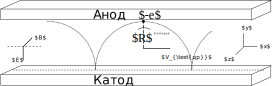
\includegraphics[width=\textwidth]{v3_3}
	\caption{Движение заряда в скрещенных полях}
	\figmark{Crossed fields}
\end{figure}
\todo[inline,author=Popov]{Рисунок странный. Что там по центру? Надо бы нарисовать другой}

Для уяснения идеи метода магнетрона, рассмотрим вначале движение заряда в
<<плоском магнетроне>>, который можно
представить себе в виде плоского конденсатора, помещённого в магнитное поле так,
что $\vec{E}\bot\vec{B}$ (рис.~\figref{Crossed fields}). При этом отрицательная
пластина конденсатора играет роль катода, положительная соответственно анода.
Если бы магнитного поля не было, то все электроны, вылетевшие без начальной
скорости из катода такого плоского диода, попадали бы на анод. При наличии
магнитного поля траектории электронов искривляются, вследствие чего при
достаточно большом магнитном поле ни один электрон не достигнет анода. Для
заданного напряжения между катодом и анодом существует некоторое критическое
значение магнитной индукции~$B_\text{кр}$, при котором траектории касаются
поверхности анода. Если~$B<B_\text{кр}$, то все электроны достигают анода и ток
через магнетрон имеет то же значение, что и без магнитного поля. Если же
$B>B_\text{кр}$, то электроны не достигают анода и ток через лампу равен нулю.

Рассчитаем это критическое значение индукции магнитного поля. Уравнения движения
электрона в нашем случае имеет вид
\begin{equation}
	\eqmark{3.9}
	m\frac{dv_x}{dt}=ev_y B,
\end{equation}
\begin{equation}
	\eqmark{3.10}
	m\frac{dv_y}{dt}=eE-ev_x B
\end{equation}
при начальных условиях $x(0)=y(0)=0$, $v_x(0)=v_y(0)=0$.

Непосредственной подстановкой несложно убедиться в том, что решением системы
дифференциальных уравнений с заданными
начальными условиями является уравнение циклоиды (в параметрической форме):
\begin{equation}
	\eqmark{3.11}
	x = vt - R\sin\omega t,\qquad y = R(1-\cos\omega t),
\end{equation}
где $ v=E/B$, $R=v/\omega=Em/(eB^2)$.

Касание анода происходит при $2R=d$ ($d$~--- расстояние между анодом и катодом).
Этому значению соответствует
критическое поле
\begin{equation}
	B_\text{кр}=\frac{\sqrt{2V}}{d\sqrt{e/m}}.
	\eqmark{3.12}
\end{equation}
Из последней формулы находим удельный заряд:
\begin{equation}
	\eqmark{3.13}
	\frac{e}{m}=\frac{2V}{d^2B_\text{кр}^2}.
\end{equation}
\todo[inline,author=Popov]{Убрать детали в описание работы. Во введении ---
    только общие соотношения}

Эта формула позволяет вычислить~$e/m$, если при заданном значении напряжения на
аноде~$V$ найти такое значение
магнитного поля, при превышении которого ток в магнетроне отсутствует.
\todo[inline,color=cyan]{<---}


\introsection{Электрический ток в вакуумном диоде}

\todo[inline,author=Popov]{Текст написан плохо и изыточно. Можно короче и лучше --->}
Электрический ток в вакуумном диоде представляет собой упорядоченное движение
электронов, испускаемых катодом. Явление испускания электронов поверхностью
твёрдого тела или жидкости называется \term{электронной эмиссией}.
Существует несколько видов электронной эмиссии. В~частности, в случае
испускания электронов поверхностями нагретых тел эмиссия называется
\term{термоэлектронной}.

Для удаления электрона из твёрдого вещества в вакуум необходимо совершить работу.
Работу по переводу электрона в свободное состояние с нулевой кинетической
энергией называют \term{работой выхода}. В~случае термоэлектронной эмиссии
работа выхода совершается за счёт кинетической энергии электронов,
которой они обладают внутри тела. Также работа может быть совершена внешним полем.
У~чистых металлов работа выхода составляет несколько электрон-вольт.

При повышении температуры металла увеличивается энергия теплового движения
электронов, количество быстрых электронов и заметное их количество сможет
преодолеть задерживающее электрическое поле и выйти из металла. Если приложить
электрическое поле, направленное к поверхности металла, то оно будет увлекать
вышедшие электроны и через вакуум потечёт электрический ток.
Этот ток называется \term{термоэлектронным}.

При \important{холодном} катоде ток через диод при подаче на анод
положительного потенциала практически отсутствует. Если же \important{нагреть}
катод, то в диоде возникает заметный ток. Ток прекращается при изменении
полярности батареи. Это как раз и указывает на то, что носителями тока в диоде
являются отрицательно заряженные частицы --- электроны.

Если бы все электроны, вылетающие из поверхности катода, попадали на анод, то
сила термоэлектронного тока~$I$ не зависела бы от величины приложенного
напряжения~$V$. На самом деле это не так. С~возрастанием напряжения ток растёт.
Однако возрастание идёт не пропорционально~$V$, так что закон Ома для вакуумного
диода не выполняется. Нелинейная зависимость тока от напряжения объясняется тем, что в пространстве
между катодом и анодом образуется отрицательный пространственный заряд,
изменяющий распределение потенциала в диоде.

При достижении определённого напряжения дальнейшее
нарастание тока практически прекращается. Ток достигает предельного значения,
называемого \term{током насыщения}. Величина тока насыщения определяется количеством
электронов, которое способно выйти из поверхности катода в единицу времени, и,
следовательно, увеличивается с ростом температуры. Если электрическое поле настолько
сильное, что способно отвести все эмитированные электроны, то дальнейшее
увеличение напряжения уже не приводит к увеличению термоэлектронного тока.
\todo[inline]{<--}

\todo[inline,color=green,author=Popov]{Вставить вместо текста выше -->}
Электрический ток в вакуумном диоде представляет собой упорядоченное движение
свободных электронов, испускаемых катодом. Характерной особенностью
такой системы является наличие в системе пространственного заряда. При этом
электроны, в отличие от обычного проводника, практически не испытывают
сопротивления своему движению. Как следствие, для вакуумного диода
не применим закон Ома.

Явление испускания электронов поверхностью твёрдого тела или жидкости называется
\term{электронной эмиссией}. Для удаления электрона из твёрдого вещества в
вакуум необходимо совершить работу, называемую \term{работой выхода}. По порядку
величины работа выхода составляет несколько электрон-вольт (у чистых металлов).
Один из механизмов эмиссии --- испускание электронов нагретыми телами. Такая
эмиссия называется \term{термоэлектронной}.
Работа выхода при этом совершается за счёт кинетической энергии электронов,
которой они обладают внутри тела.

Если создать электрическое поле вне металла, оно будет увлекать вышедшие
электроны и через вакуум потечёт электрический ток.
С повышением температуры поверхности экспоненциально быстро растёт доля частиц,
способных преодолеть потенциальный барьер и выйти из металла,
и следовательно растёт интенсивность эмиссии электронов. Это приводит к тому, что
в пространстве диода~--- особенно вблизи катода~--- накапливается отрицательный
объёмный заряд, экранирующий внешнее поле. Из-за этого результирующий ток в диоде
оказывается значительно меньше тока эмиссии с катода.
Такой режим работы диода называют \term{режимом объёмного заряда}.

При достижении определённого напряжения дальнейшее нарастание тока практически
прекратится~--- ток достигает предельного значения $I_{нас}$, называемого
\term{током насыщения}. Это обусловлено ограниченностью эмиссионной способности
катода~--- величина тока насыщения определяется количеством электронов,
которое способно выйти из поверхности катода в единицу времени.
\todo[inline,color=green]{<---}


\paragraph{Закон 3/2 для вакуумного диода.}
Рассмотрим режим объёмного заряда в простейшем случае \important{плоского} диода.
Его электроды представимы в виде двух параллельных плоскостей,
между которыми задано напряжение $V$. Расстояние~$d$ между электродами много
меньше их площади. Направим ось~$x$ перпендикулярно к поверхности катода
в сторону анода, совместив начало координат с поверхностью
катода. В~этой модели задача стала одномерной~--- все величины являются
функциями только координаты~$x$.

Запишем для электрического поля теорему Гаусса в дифференциальной форме:
\[
\frac{dE}{dx} = \frac{\rho}{\varepsilon_0},
\]
где~$\rho(x)$~--- плотность электрического заряда. По определению потенциала
электростатического поля имеем
\[
E = -\frac{d\varphi}{dx}.
\]
Отсюда находим, что $\varphi(x)$ удовлетворяет уравнению
\begin{equation}
	\eqmark{3.14}
	\frac{d^2\varphi}{dx^2}=-\frac{\rho}{\varepsilon_0}.
\end{equation}
Это частный (одномерный) случай \term{уравнения Пуассона}.

Плотность тока в диоде равна $j=\rho v$, где $v$~--- скорость электронов.
В стационаре заряд нигде не накапливается, поэтому плотность тока всюду одинакова: $j=\const$.
Из закона сохранения энергии имеем:
\begin{equation*}
	\frac{mv^2}{2}=e\varphi.
\end{equation*}
Здесь мы выбрали начало отсчёта потенциала на катоде, а также
пренебрегли \important{начальными тепловыми скоростями},
с которыми вылетают электроны с поверхности катода. Это можно сделать, если
приложенное напряжение достаточно велико: $eV\gg mv_{T}^2/2$.

Исключив из полученных соотношений плотность электронов~$\rho$ и скорость~$v$,
приходим к уравнению
\begin{equation}
	\eqmark{3.15}
    \frac{d^2\varphi}{dx^2}=\sqrt{\frac{m}{2e\varphi}} \frac{j}{\varepsilon_0}
\end{equation}
с граничными условиями
\begin{equation*}
 \varphi(0)=0,\qquad \varphi(d)=V.
\end{equation*}

Для однозначного решения этого дифференциального уравнения второго порядка
необходимо ещё одно граничное условие.
\todo[inline,author=Popov]{Это неправильное объяснение выбора граничного
    условия! В общем случае решения с конечными $E$ и $j$
на катоде существуют! На самом деле здесь физическое условие бесконечной
эмиссионной способности катода
--->}
 Если сопоставить уравнения \eqref{3.14} и \eqref{3.15}, то можно сделать вывод
об обращении плотности заряда на катоде в бесконечность. Точка~$x=0$ является
особой точкой уравнения \eqref{3.15}, в которой оно теряет смысл. Это связано с
тем, что мы пренебрегли тепловыми скоростями на катоде, приняв их равными нулю.
Оказывается, что в этой модели плотность тока через диод получается конечной,
только если напряжённость поля у катода равна нулю.
Это условие означает, что поле возникающего вблизи катода пространственного заряда полностью экранирует
электрическое поле, создаваемое разностью потенциалов между анодом и катодом.
Таким образом, получаем второе граничное условие в виде
\begin{equation*}
    \left.\frac{d\varphi}{dx}\right|_{x = 0}=0.
\end{equation*}
\todo[inline]{<---}

\todo[inline,author=Popov,color=green]{Вставить этот текст --->}
В общем случае это должна быть связь между плотностью тока~$j$ и электрическим
полем на поверхности катода $E_0 = -\left.\frac{d\varphi}{dx}\right|_{x=0}$,
которую однако  теоретически установить затруднительно.
Учтём, что в режиме объёмного заряда количество электронов, способных покинуть
катод из-за его нагрева, значительно превосходит ток в диоде.
Следовательно, \important{эмиссионная способность катода практически не ограничена},
поэтому чтобы плотность тока оставалась конечной,
напряжённость электрического поля внутри катода нужно устремить к нулю, $E_0\to 0$.
Таким образом, получаем второе граничное условие в виде
\begin{equation*}
    \left.\frac{d\varphi}{dx}\right|_{x = 0}=0.
\end{equation*}

Прямой подстановкой можно проверить, что решением \eqref{3.15},
удовлетворяющим данным граничным условиям, является функция вида
\begin{equation*}
    \varphi^{3/2} =\const \cdot j x^2.
\end{equation*}
Подставляя $\varphi(d)=V$, получим связь между током и напряжением
(вольт-амперную характеристику) в вакуумном диоде:
\begin{equation}
    I \propto V^{3/2}.
\end{equation}
Это так называемый <<\term{закон 3/2}>> \term{Чайлда--Ленгмюра}.

Как следует непосредственно из проведенного вывода,
в реальной системе <<закон 3/2>> нарушается как при слишком малых напряжениях,
когда нельзя пренебрегать начальными тепловыми скоростями электронов,
так и при слишком больших напряжениях, когда диод переходит в режим насыщения.
В~промежуточной области закон хорошо подтверждается на опыте, в том числе
и для электродов неплоской геометрии.
\todo[inline,color=green]{<---}

\todo[inline,author=Popov,color=cyan]{Убрать в описание работы и там дополнить --->}
Теперь задача о распределении потенциала становится однозначной и приводит к
решению
\begin{equation*}
	j=\frac{4\varepsilon_0}{9x^2}\sqrt{\frac{2e}{m}}\varphi^{3/2}.
\end{equation*}
\todo[inline,author=Popov]{Убрать детали в описание работы,
во введении --- только общие законы}

Так как $\varphi(d)=V$, где~$d$~--- расстояние между электродами, то для
зависимости тока от напряжения получаем
\begin{equation*}
	I=\frac{4\varepsilon_0 S}{9d^2}\sqrt{\frac{2e}{m}}V^{3/2},
\end{equation*}
где~$S$~--- площадь катода. Мы получили зависимость тока через плоский диод от
приложенного к нему напряжения, известную как <<закон трёх вторых>> для плоского
диода. Оказывается, что не только для плоского вакуумного диода, а и для
вакуумного диода с электродами любой другой геометрии ток подчиняется <<закону
степени трёх вторых>>.

Полученная формула подсказывает процедуру измерения удельного заряда электрона.
Для этого достаточно по
результатам эксперимента построить график зависимости тока от напряжения в
степени трёх вторых, который должен
представлять собой прямую линию, проходящую через начало координат. Угол наклона
этой прямой линии пропорционален (с известным коэффициентом) квадратному корню
из~$e/m$~--- искомой величины удельного заряда электрона.
\todo[inline,color=cyan]{<---}

\introsection{Свободные носители заряда в металлах и~полупроводниках}

Проводимость большинства твёрдых тел связана с движением электронов. Электроны
входят в состав атомов всех тел, однако одни тела не проводят электрический ток
(диэлектрики), а другие являются хорошими его проводниками. Причина различия
заключается в особенностях энергетического состояния внешних электронов атомов в
этих веществах.

При объединении атомов в твёрдое тело (кристалл) внешние электроны теряют связь
со <<своими>> атомами и теперь принадлежат всему кристаллу в целом. Каждому
уровню энергии электрона одиночного атома соответствует в кристалле группа
близких по энергии уровней (разрешённая зона), в которой число уровней равно
числу мест на соответствующем атомном уровне, умноженному на число атомов в
кристалле. Число уровней, объединившихся в зону, при слиянии не меняется. Оно
определяет максимальное число электронов, которое может <<поместиться>> в зоне
(в силу принципа Паули).

Если одна из энергетических зон до конца заполнена электронами, а следующая зона
совершенно пуста, то под действием слабого внешнего электрического поля
электронам некуда перетекать, и вещество является \important{диэлектриком}.
Верхняя из заполненных зон называется \important{валентной зоной}.

Положение меняется, если в кристалле имеется зона, частично заполненная
электронами. В~этом случае внешнее электрическое поле может изменить
распределение электронов по уровням энергии и создать упорядоченное движение
электрических зарядов. Частично заполненная зона называется \important{зоной
проводимости}. Частично заполненная электронами зона имеется у всех твёрдых
проводников электрического тока; в том числе её имеют все металлы.

Если ширина запрещённой зоны относительно невелика, тепловое движение
перебрасывает часть электронов из валентной зоны в свободную~--- зону
проводимости. При этом в зоне проводимости появляются электроны, а в валентной
зоне~--- свободные места~--- \important{дырки}. Электроны в зоне проводимости и
дырки валентной зоны участвуют в переносе заряда. Такие вещества называются
\important{полупроводниками}. Обычно к полупроводникам относят материалы с
шириной запрещённой зоны $\Delta E \lesssim 2$~эВ. Число носителей тока в
полупроводниках экспоненциально увеличивается с~повышением температуры.

Рассматривая коллективное движение электронов почти заполненной зоны, полезно
мысленно заполнить свободные места
воображаемыми парами, состоящими из электронов с одинаковыми по величине
положительным и отрицательным зарядами. Обычныеотрицательные заряженные
электроны заполняют теперь все уровни и, следовательно, не могут принимать
участия в проводимости. Они образуют структуру, характерную для изоляторов.
Проводимость связана только с введёнными нами
<<электронами>>, обладающими положительным зарядом. Такие <<электроны>> носят
название \important{дырок}. При рассмотрении явлений, происходящих в~металлах
с~почти заполненной валентной зоной, удобно представлять себе дело так, как если
бы проводниками тока были не настоящие электроны, а положительно заряженные
дырки. В~этом случае говорят о \important{дырочном типе проводимости.}

Электронным типом проводимости обладает большинство чистых металлов. Однако в
ряде металлов (бериллий, кадмий и
некоторые другие) основными носителями электрического тока являются дырки. Это
связано с особенностями их зонной
структуры.

\introsubsection{Эффект Холла}

Рассмотрим прохождение тока в рамках модели свободных электронов.
Закон Ома в дифференциальной форме выражает связь векторов~$j$~--- плотности тока
и~$E$~--- электрического поля:
\begin{equation}
	j=\lambda E.
	\eqmark{3.16}
\end{equation}

В~нулевом магнитном поле, если проводящая среда изотропна (то есть не имеет
выделенных направлений), проводимость~$\lambda$ является числом (скаляром). Это
значит, что векторы~$j$ и~$E$ сонаправлены. В~общем же случае
$\widehat{\lambda}$ является тензором второго ранга, то есть матрицей, при
умножении которой на вектор~$E$ получается вектор~$j$. В~присутствии магнитного
поля эта матрица становится недиагональной в результате эффекта Холла. Тензор
удельного сопротивления~$\widehat{\rho}$ является обратным к тензору
проводимости: $E=\widehat{\rho}j$, то есть
$\widehat{\rho}=\widehat{\lambda}^{-1}$.
\todo[inline,author=Popov]{Как-то слишком резко --- бац и тензор. Нужно
    дать более гуманное введение в тему}

Электроны в металлах и легированных полупроводниках движутся с большими
скоростями во всех направлениях, а под действием тянущего
электрического поля приобретают ненулевую среднюю скорость дрейфового движения
$v_{dr}=  Eb$, где~$b$~--- подвижность.

\todo[inline,author=Popov]{Дать чёткое определение эффекту Холла и
    магнито(или магнето?)-сопротивлению}
Разберем магнитосопротивление и эффект Холла на микроуровне. Если магнитное поле
направлено вдоль тока, то
оно не влияет на ток, поскольку сила Лоренца равна нулю. Поэтому мы рассмотрим
случай, когда поле перпендикулярно
току. Пусть рассматриваемая система для простоты содержит носители только одного
сорта (большинство металлов
являются хорошими примерами).
\begin{figure}[h!]
	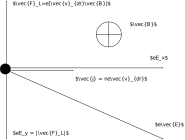
\includegraphics[width=0.9\textwidth]{Chapter_3/Hall_forces}
	\caption{Силы, действующие на носитель заряда в проводящей среде в тянущем
электрическом и перпендикулярном ему магнитном полях.}
	\figmark{Hall forces}
\end{figure}

Если в системе локально течет ток электронов $j_x=nev_{dr\, x}$, направленный
вдоль оси~$x$, а магнитное поле~$B$ направлено вдоль оси~$z$, то на заряды
действует действует сила Лоренца $ F_{L}=e[v_{dr}B]$ вдоль оси~$y$.
Сила Лоренца должна приводить к образованию компоненты тока вдоль оси~$y$, но по
условиям ток течет вдоль~$x$. Это значит, что заряды должны перераспределиться
таким образом, чтобы полностью скомпенсировать силу
Лоренца, создав в~$y$ направлении электрическое холловское поле $E_y=v_{dr}B$.
Поскольку сила Лоренца
оказывается полностью скомпенсирована $eE_y$, то электрон движется так, как если
бы магнитного поля не
было, то есть $j_x=E_xbne$, $j_y=j_z=0$. Это позволяет написать в явном виде
тензор удельного сопротивления:
\begin{equation}
	\widehat{\rho}(B)=\frac{1}{bne}\left(
	\begin{tabular}{ccc}
		{\it 1} & {\it bB} & {\it 0} \\
		{\it -bB} &{\it 1}& {\it 0} \\
		{\it 0} &{\it 0}& {\it 1}\\
	\end{tabular}
	\right).
	\eqmark{3.17}
\end{equation}

Здесь коэффициент, стоящий перед матрицей,
\begin{equation}
	\frac{1}{bne} = \rho_0
	\eqmark{UdSoprot}
\end{equation}
есть удельное сопротивление полупроводника при отсутствии магнитного поля.

Обращением этой матрицы нетрудно получить тензор проводимости:
\begin{equation}
	\widehat{\lambda}(B)=\frac{bne}{1+b^2B^2}\left(
	\begin{tabular}{ccc}
		{\it 1} & {\it bB} & {\it 0} \\
		{\it -bB} &{\it 1}& {\it 0} \\
		{\it 0} &{\it 0}& {\it 1}\\
	\end{tabular}
	\right).
	\eqmark{3.18}
\end{equation}

Существуют две основных и принципиально различных геометрии для исследования
магнитосопротивления: геометрия
мостика Холла и геометрия диска Корбино (см. рис.~\figref{Geometries}).

В~геометрии мостика Холла ток вынуждают течь вдоль образца, сила Лоренца
прибивает носители к краю образца, создавая тем самым холловское поле, которое
компенсирует силу Лоренца. Напряжение между точками $V_{xy}$ равно~$E_yw$, где,
согласно уравнению \eqref{3.17}, $E_y=\rho_{yx}\times j_x=j_x B/(ne)$. Плотность
тока, текущего через образец, равна полному току~$I$, деленному на площадь
поперечного сечения образца~$wh$. Таким образом, для холловского напряжения
имеем:
\begin{equation}
	V_{xy}=\frac{IB}{neh}.
	\eqmark{3.19}
\end{equation}

В~этой же модели для падения напряжения вдоль образца имеем:
\begin{equation}
	V_{xx}=\frac{Il}{nebwh}.
	\eqmark{3.20}
\end{equation}

Tаким образом, удельное сопротивление~$\rho_{xx}$ образца не зависит от
магнитного поля (магнитосопротивление равно 0). Этот факт объясняется тем, что
сила Лоренца и сила ЭДС Холла (рис. \figref{Hall forces}) полностью
уравновешивают друг друга. В~реальных системах, тем не менее, предположения
модели не выполняются и магнитосопротивление зачастую отлично от 0. Причины
могут быть различными:
\begin{enumerate}
\item Система может быть анизотропной, то есть в разных направлениях ($x,y,z$)
токопроводящие свойства различны. В~этом случае величина силы Лоренца содержит
не среднюю дрейфовую скорость, а зависит от направления большой мгновенной
скорости электрона.

\item Система может быть многокомпонентной. Например, в полупроводниках часто
одновременно существуют электроны и дырки, концентрации ($n$ и~$p$) и
подвижности ($b_n$ и~$b_p$) которых в общем случае различаются. Тогда полный
тензор проводимости будет суммой тензоров проводимости двух компонент вида
\eqref{3.18}. Обращением тензора проводимости в пределе малых магнитных полей
можно показать, что холловское сопротивление двухкомпонентной системы в
полупроводнике равно:
\begin{equation}
	R_{xy}\equiv \frac{V_{xy}}{I}=\frac{n{b_n}^2-p{b_p}^2}{eh(nb_n+pb_p)^2}B
	\eqmark{3.21}
\end{equation}

\item Существуют квантовые эффекты в проводимости, которые приводят к тому, что
подвижность зависит от магнитного поля. Например если сам проводящий материал
является ферромагнетиком, то с ростом поля он намагничивается, количество
доменов уменьшается, а доменные стенки являются причиной сильного рассеяния, то
есть уменьшают подвижность.
\end{enumerate}

Поскольку холловское сопротивление содержит толщину образца~$h$, то договорились
называть холловское сопротивление, умноженное на толщину образца, постоянной
Холла. Постоянная Холла характеризует материал, так как зависит только от
концентрации носителей в нем:
\begin{equation}
	R_x=\frac{1}{ne}
	\eqmark{HallConstant}
\end{equation}
или от соотношений между концентрациями и подвижностями, если в материале
несколько типов носителей. В~таблице в приложении даны постоянные Холла для
различных металлов. Для полупроводников постоянные Холла сильно зависят от
наличия малых концентраций примеси и температуры.

Отдельно следует упомянуть, что существуют двумерные системы (например, графен),
в которых движение носителей заряда происходит только в плоскости, а движение в
перпендикулярном направлении квантовомеханически запрещено. В~этих системах
концентрация измеряется в количестве носителей на единицу площади, а холловская
постоянная есть просто холловское сопротивление, делённое на магнитное поле. В
двумерных системах тензоры в формулах \eqref{3.17} и \eqref{3.18} содержат
только~$x$ и~$y$ компоненты, то есть являются матрицами~$2\times2$.
\todo[inline, author=Popov]{А стоило ли отдельно упоминать графен,
    прерывая повествование? Лирические
    отступления вынести в конец или в начало раздела}

Измерения в геометрии мостика Холла представляют собой четырехконтактные
измерения, то есть два контакта используются для задания тока через образец, а с
двух контактов снимается падение напряжения. Поскольку вольтметр обладает
бесконечным сопротивлением (то есть ток через него не течет), измеряемое падение
напряжения совершенно не зависит от свойств контактов, а определяется только
свойствами материала.

Геометрия диска Корбино представляет собой двухточечную схему, то есть
сопротивление образца в ней суммируется с сопротивлениями контактов. Поэтому
исключительно важно создать низкоомные контакты к образцу, сопротивлением
которых можно пренебречь. В~геометрии Корбино из-за аксиальной симметрии не
формируется холловское напряжение. Электрическое поле направлено строго по
радиусу системы. В~магнитном поле ток вынужден протекать под углом к
электрическому полю, то есть по спирали. Из-за симметрии полный ток включает
только компоненту вдоль радиуса $j_r=\lambda_{xx} E_r$. Плотность тока может
быть выражена через полный ток и толщину образца $j_r=I/(2\pi rh)$.
Теперь запишем для напряжения:
\begin{equation*}
V={\int_{r_1}}^{r_2}E_r dr={\int_{r_1}}^{r_2}\frac{j_r}{\lambda_{xx}}
dr={\int_{r_1}}^{r_2}I\rho_0\frac{1+b^2B^2}{2\pi
rh}dr=I\rho_0\frac{1+b^2B^2}{2\pi h}\ln{\frac{r_2}{r_1}}.
\end{equation*}
\todo[inline,author=Popov]{Убрать этот ужас в описание работы}

Если система однокомпонентная, то магнетосопротивление в геометрии Корбино есть
\begin{equation}
	R(B) = R_0(1+b^2B^2)
	\eqmark{MagnetoSoprot}.
\end{equation}

Здесь
\begin{equation}
	R_0 = \frac{\rho_0}{2\pi h} \ln{\frac{r_2}{r_1}}
	\eqmark{KorbinoSoprot}
\end{equation}

Для наблюдения этого магнитосопротивления выбирают систему с большой подвижнотью
носителей (как правило, это полупроводник с низкой эффективной массой электронов
типа InSb).

\begin{figure}[h!]
	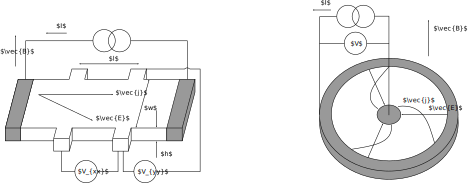
\includegraphics[width=0.9\linewidth]{Chapter_3/2schemes}
	\caption{Две геометрии для исследования влияния магнитного поля на
проводящие свойства: мостик Холла (слева) и диск Корбино (справа).}
	\figmark{Geometries}
\end{figure}

При наложении внешнего электрического поля~$E$ электроны начинают ускоряться.
Однако после некоторого <<свободного пробега>> происходит соударение с решёткой,
электрон теряет набранную энергию, и процесс ускорения начинается заново.
Соударения с решёткой, подобно вязкому трению, приводят к тому, что
результирующее движение электрона можно описать некоторой средней скоростью
$\left< v \right>$, пропорциональной внешнему полю:
\begin{equation}
	\eqmark{3.22}
	\left< \vec{v} \right>=-b\vec{E}.
\end{equation}

\todo[inline,author=Popov]{Что это? Куски старого текста? Раздел остро
    нуждается в редактировании!}

Введённая здесь величина~$b$ называется \important{подвижностью}. В~определённых
пределах изменения температуры,
напряжённости поля и его частоты эта характеристика вещества остаётся постоянной
и приводится в справочниках. Для
положительно заряженных носителей тока в формуле \eqref{3.22}, очевидно, стоит
знак <<плюс>>.

При установившемся движении средняя сила, действующая на электроны со стороны
кристаллической решётки, равна внешней силе~$-eE$ и направлена в противоположную
сторону. Поэтому действие кристаллической решётки на движение электронов в
среднем эквивалентно силе трения, пропорциональной скорости:
\begin{equation}
	\eqmark{3.23}
	F_\text{тр}=-\frac{e}{b}\average{\vec{v}}.
\end{equation}

Если концентрация электронов равна~$n$, величина плотности тока определится
очевидным соотношением
\begin{equation}
	\eqmark{3.24}
	j=en\average{v}=enbE.
\end{equation}

Таким образом, выполняется закон Ома~--- величина плотности тока~$j$
пропорциональна напряжённости поля~$E$:
\begin{equation}
	\eqmark{3.25}
	j=\sigma E.
\end{equation}

Сравнивая \eqref{3.24} и \eqref{3.25}, получаем выражение для проводимости
\begin{equation}
	\eqmark{3.26}
	\sigma=enb.
\end{equation}

Химически чистые полупроводники обладают проводимостью, которая связана с
небольшим числом электронов в зоне
проводимости и таким же числом дырок в валентной зоне. Такая проводимость
называется собственной~--- она не связана с примесями. Добавление небольшого
количества специально подобранных примесей (так называемое
легирование) может существенно увеличить проводимость полупроводников или даже
создать ощутимую проводимость при комнатной температуре в веществах с
запрещённой зоной, ширина которой заметно превышает 2~эВ. Такое происходит,
когда атомы примеси имеют энергетические уровни в запрещённой зоне основного
материала.

Если заполненные примесные уровни расположены вблизи потолка запрещённой зоны,
находящиеся на этих уровнях электроны легко переходят в зону проводимости.
Наоборот, на свободные уровни у дна зоны проводимости легко переходят электроны
валентной зоны с образованием в этой зоне дополнительного количества дырок. В
обоих случаях число переносчиков заряда увеличивается, и проводимость
возрастает. В~первом случае говорят о полупроводниках \important{электронного},
или $n$-типа, а во втором~--- о  полупроводниках дырочного, или $p$-типа. В
общем случае в процессе электрической проводимости участвуют как электроны, так
и дырки. Удельная электрическая проводимость полупроводника при этом равна
\begin{equation}
	\eqmark{3.27}
	\sigma=e(nb_e+pb_p),
\end{equation}
где~$n$ и~$p$~--- концентрации электронов и дырок, а~$b_e$ и~$b_p$~--- их
подвижности. В~случае \important{примесной
проводимости} один тип носителей обычно существенно преобладает над другим и в
формуле \eqref{3.27} можно пренебречь одним из слагаемых.



\begin{lab:literature}
	\item{ \emph{Сивухин Д.В.} Общий курс физики.~--- T.~III. Электричество.~---
М.: Наука, 1983. \S\S~86, 95, 98, 100.}
	\item{ \emph{Кингсеп А.С., Локшин Г.Р., Ольхов О.А.} Основы физики.
Т.~1.~--- М.: Физматлит, 2001. \S\S~8.1--8.3.}
\end{lab:literature}




\newpage

\lab{Измерение удельного заряда электрона методами магнитной фокусировки и
магнетрона}

\aim{определение отношения заряда электрона к его массе методом магнитной
фокусировки и методом магнетрона.}

\equip{А)~электронно-лучевая трубка (с блоком питания), соленоид, 
    регулируемый источник постоянного тока, вольтметр, 
    магнитометр (миллитесламетр или милливеберметр);
Б)~электронная лампа с цилиндрическим анодом, 
регулируемый источник постоянного тока, соленоид, вольтметр, два амперметра.}

Перед выполнение работы необходимо ознакомиться с теоретическим введением
к Разделу (п. \ref{sec:freemotion}).

\labsection{А.~Метод магнитной фокусировки}


В постоянном однородном магнитном поле траектории заряженных частиц представляют
собой спирали, радиус которой определяется формулой \chaptereqref{3.4}.
За время $T_B= \frac{2\pi r_B}{v_{\perp}}$, которое можно назвать
\term{циклотронным периодом}, заряд сместится вдоль магнитного поля на 
расстояние $L$ (шаг спирали):
\begin{equation}
    \eqmark{3.6}
    L = v_{\parallel}T_B =\frac{2\pi v\cos\alpha}{(e/m)B},
\end{equation}
где $\alpha$ --- угол между вектором скорости $\vec{v}$ и направлением поля $\vec{B}$.
Если углы малы, $\alpha \ll 1$, то $\cos\alpha \approx 1$ и
\begin{equation}
    \eqmark{3.7}
    L \approx \frac{2\pi v}{(e/m)B}.
\end{equation}
Таким образом, при малых углах расстояние~$L$ не зависит от~$\alpha$, так
что все электроны, вышедшие из одной точки, после одного оборота вновь соберутся
в одной точке~--- \emph{сфокусируются}. Как следует из \eqref{3.7}, 
индукция поля~$B$, при которой точка фокусировки отстоит от точки вылета 
на расстоянии~$L$, определяется величиной~$e/m$~--- удельным зарядом частицы.

В работе исследуется пучок электронов, создаваемый электронно-лучевой трубкой, 
помещённой в магнитное поле соленоида.
Скорость движения электронов определяется разность потенциалов~$U$,
пройденную им до попадания в магнитное поле:
\begin{equation*}
  \frac{mv^2}{2}=eU,
\end{equation*}
откуда
\begin{equation}
  \eqmark{3.3}
  v=\sqrt{\frac{2eU}{m}}.
%   = 6\cdot10^5\sqrt{V}~\frac{m}{c}.
\end{equation}

Пусть $B_{ф}$ --- индукция поля, при которой наступает фокусировка.
Из \eqref{3.3} и \eqref{3.7} выразим удельный заряд электрона~$e/m$
через $B_{ф}$:
\begin{equation}
\eqmark{3.8}
\frac{e}{m}=\frac{8\pi^2 U}{L^2B_{ф}^2}.
\end{equation}
Эта формула и лежит в основе экспериментального измерения удельного заряда
электрона по \important{методу магнитной фокусировки}.

\experiment 

Основной частью установки является электронный осциллограф, трубка
которого вынута и установлена в длинном соленоиде, создающим магнитное поле,
 направленное вдоль оси трубки. 
Вылетая с катода, электроны имеют разные скорости (тепловая энергия $\sim 0,1\;эВ$).
Однако далее они ускоряются большой анодной разностью потенциалов ($U_А~\sim 1\;кВ$) и отсеиваются
на двух диафрагмах, благодаря чему получается пучок частиц с малой расходимостью
по углу ($\Delta \alpha \ll 1$) и практически одинаковыми продольными скоростями
$v_{\parallel}=\sqrt{2eU_А/m}$.

В магнитном поле соленоида все электроны будут двигаться по спиралям 
с практически одним и тем же шагом~$L$
(см. \eqref{3.6}), и, следовательно, будут встречаться вновь, 
пересекая ось пучка на расстояниях~$nL$, $n=1,\,2,\,3,\ldots$
В~этих точках сечение пучка будет наименьшим, и при изменении магнитного 
поля изображение пучка на экране будет периодически стягиваться 
в ярко светящуюся точку. 
Таким образом, удельный заряд может быть получен из соотношения
\begin{equation}
\frac{e}{m}=\frac{8\pi^2U}{L^2}\cdot\frac{n^2}{B_ф^2(n)}.
\eqmark{3.1.1}
\end{equation}

\begin{figure}[h]
    \centering
	\pic{6cm}{Chapter_3/3_1_1}
	\caption{Схема измерений по~методу магнитной фокусировки}
	\figmark{Magnetic focusing scheme}
\end{figure}

Анодное напряжение, определяющее продольную скорость электронов, измеряется
вольтметром. Магнитное поле в соленоиде создаётся постоянным током
(рис.~\figref{Magnetic focusing scheme}), сила которого задается источником
питания постоянного тока и измеряется амперметром~A источника. Ключ~К
служит для изменения направления поля в соленоиде.

Величина магнитного поля определяется с помощью магнитометра, датчик которого
расположен внутри соленоида. В~качестве магнитометра может использоваться
\emph{милливеберметр} (\emph{флюксметр}), у которого датчиком является 
измерительная катушка, намотанная на один каркас с соленоидом. 
Таким образом измеряется изменение магнитного потока,
пронизывающего измерительную катушку. Описание милливеберметра и правила работы
с ним приведены на с.~\pageref{MWB}. Альтернативно индукция поля может измеряться
миллитесламетром (датчиком Холла).

На точность результатов может влиять внешнее магнитное поле, особенно
продольное. Оно не вызывает размытия фокуса, но изменяет величину фокусирующего
поля. Присутствие внешнего магнитного поля проще всего обнаружить с помощью
переполюсовки соленоида: при изменении направления поля показания
милливеберметра будут отличаться, но их полусумма не зависит от наличия
постоянного продольного поля.

Измерение магнитного поля производится в предварительных опытах: 
при отключенном ключе~К устанавливается связь между силой тока, протекавшего через
соленоид, и индукцией магнитного поля в соленоиде. 
По измеренным значениям строится \emph{калибровочный график} $B(I)$, 
который используется при обработке результатов
основных измерений для пересчёта индукции магнитного поля по известному току.

\begin{lab:task}

Измерьте значения магнитных полей, при которых происходит фокусировка 
электронного пучка, и по результатам измерений рассчитайте удельный
заряд электрона $e/m$.

\begin{enumerate}
    
\item Ознакомьтесь с назначением ручек источника питания и с устройством 
    используемого в работе магнитометра. 
    
\item Измерьте калибровочную кривую $B(I)$ зависимости магнитного поля
от тока через соленоид. В~случае использования установки с
милливеберметром,~$B$ вычисляется через поток $\Phi=BSN$, пронизывающего пробную
катушку (значение параметра~$SN$ катушки указано на установке).

Проведите измерения во всём доступном диапазоне изменения тока при двух
направлениях тока через обмотку.

\item При минимальном или нулевом токе через соленоид включите осциллограф и
подайте напряжение с внешнего или внутреннего генератора на вертикальный (или
горизонтальный) вход усилителя. На экране появится светящаяся линия.

\item Постепенно увеличивая ток через соленоид, найдите значение тока~$I_ф$, при
котором линия в первый раз стягивается в точку (сила тока~$I_ф$ зависит,
конечно, от ускоряющего напряжения~$U_А$, которое в свою очередь пропорционально 
яркости луча, поэтому не следует настройку яркости до конца измерений).

Продолжая увеличивать ток, получите зависимость~$I_ф(n)$ от порядкового номера
фокуса~$n$.

\item Повторите измерения $I_ф(n)$ для обратного направления магнитного поля
в соленоиде.

\item Запишите значение ускоряющего напряжения~$U_А$, длину трубки
$L$ и характеристики приборов.

\item Установите регуляторы источника питания на минимум и выключите его. 
Выключите осциллограф.

\end{enumerate}

\tasksection{Обработка результатов}

\begin{enumerate}
\item Постройте калибровочный график $B(I)$.

\item Пользуясь графиком $B(I)$ определите усреднённые значения~$B_ф$ для каждого
фокуса и постройте график зависимости $B_ф(n)$ фокусирующего поля от номера $n$. 
Используйте наклон графика для расчёта~$e/m$ с помощью формулы~\eqref{3.1.1}.

\item Оцените погрешности и сравните результат с табличным.

\end{enumerate}
\end{lab:task}

\labsection{Б. Измерение ${e/m}$ методом магнетрона}

В~так называемом {\important{методе магнетрона}} отношение~$e/m$ измеряется на
основе исследования движения электрона в перпендикулярных друг другу (скрещенных) 
электрическом и магнитном полях. Название метода связано с тем, что такая
конфигурация полей реализуется в магнетронах~--- 
генераторах электромагнитных колебаний сверхвысоких частот.

\begin{figure}[h!]
    \centering
    \pic{8cm}{Chapter_3/v3_3}
    \caption{Движение заряда в скрещенных полях (без начальной скорости)}
    \figmark{Crossed fields}
\end{figure}
%\todo[inline,author=Popov]{Рисунок странный. Что там по центру? Надо бы
%    нарисовать другой}

Для уяснения идеи метода магнетрона, рассмотрим вначале упрощённую
задачу о движение заряда в <<плоском магнетроне>>. 
Пусть имеется плоский конденсатор, в пространстве между пластинами которого создан
высокий вакуум (вакуумный диод). Поместим его в однородное магнитное поле (например,
внутрь соленоида) так, что $\vec{E}\perp\vec{B}$ (рис.~\figref{Crossed fields}). 
При этом отрицательная пластина конденсатора играет роль катода, 
положительная~--- анода. Если бы магнитного поля не было, то все электроны, 
вылетевшие без начальной скорости из катода, попадали бы на анод. 
При наличии же магнитного поля траектории электронов искривляются, 
вследствие чего при достаточно большом $B$ ни один электрон не достигнет анода.
Таким образом, при
заданном напряжения $V$ между пластинами существует некоторое критическое
значение магнитной индукции~$B_\text{кр}(V)$, при котором траектории касаются
поверхности анода. Если~$B<B_\text{кр}$, то все электроны достигают анода и ток
через магнетрон имеет то же значение, что и без магнитного поля. Если же
$B>B_\text{кр}$, то электроны не достигают анода и ток через диод равен нулю.

Рассчитаем это критическое магнитное поле для плоского конденсатора.
Движение электрона будет иметь характер электрического дрейфа. 
Если начальная скорость равна нулю 
(начальные условия $x(0)=y(0)=0$, $v_x(0)=v_y(0)=0$), 
то как нетрудно получить из уравнений \chaptereqref{3.9}, 
траекторией частицы будет \emph{циклоида}:
\begin{equation}
\eqmark{3.11}
x = Vt - R\sin \omega_B t,\qquad y = R(1-\cos\omega_B t),
\end{equation}
где $V=E/B$ --- дрейфовая скорость, $R=V/\omega_B=Em/(eB^2)$.
Касание анода происходит при $2R=h$ ($h$~--- расстояние между анодом и катодом).
Этому значению соответствует критическое поле
\begin{equation}
B_\text{кр}=\frac{\sqrt{2U}}{h\sqrt{e/m}},
\eqmark{3.12}
\end{equation}
где $U=Eh$ --- напряжение между пластинами.
Отсюда находим удельный заряд:
\begin{equation}
\eqmark{3.13}
\frac{e}{m}=\frac{2U}{h^2B_\text{кр}^2}.
\end{equation}

Формула \eqref{3.13} позволяет вычислить~$e/m$, если при заданном 
значении напряжения на диоде~$U$ найти такое значение
магнитного поля, при превышении которого ток в магнетроне отсутствует.

\experiment

\begin{figure}[h!]
	\begin{minipage}[b]{0.49\textwidth}
		\pic{0.9\textwidth}{Chapter_3/3_1_2}
		\caption{Схема устройства двухэлектродной лампы}
		\figmark{Two-electrode lamp}
	\end{minipage}
	\hfill
	\begin{minipage}[b]{0.49\textwidth}
		\pic{0.9\textwidth}{Chapter_3/3_1_3}
		\caption{Траектории электронов, вылетающих из~катода, при~разных
значениях индукции магнитного~поля}
		\figmark{Path of electrons}
	\end{minipage}
\end{figure}

В данной работе движение электронов случае происходит в кольцевом пространстве,
заключённом между катодом и анодом двухэлектродной электронной вакуумной лампы 
(рис.~\figref{Two-electrode lamp}).
Нить накала лампы (катод) располагается вдоль оси цилиндрического анода, так что
электрическое поле между катодом и анодом имеет \emph{радиальное} направление. 
Лампа помещается внутри соленоида, создающего магнитное поле, \emph{параллельное оси} лампы.

Таким образом, реализуется геометрия скрещенных полей $\vec{E}$ и $\vec{B}$.
Поскольку поле $\vec{E}$ в данном случае не является однородным (оно зависит от расстояния
до оси), траектории частиц будут несколько отличаться от рассмотренного выше плоского
случая. Тем не менее, все качественные особенности траектории сохранятся:
выражение для критического поля будет отличаться от \eqref{3.12} только
численным коэффициентом порядка единицы.
Подробно задача о движении электронов в такой лампе рассмотрено в приложении к работе.
В частности, там получено следующая связь критического поля 
$B_{кр}$ и напряжения на лампе $U_{А}$:
\begin{equation}
    B_\text{кр}=\frac{2\sqrt{2U_{А}}}{r_{А}\sqrt{e/m}},
	\eqmark{3.1.2}
\end{equation}
где $r_{А}$~--- радиус анода. Для удельного заряда имеем
\begin{equation}
	\frac{e}{m}=\frac{8U_{А}}{B_\text{кр}^2r_{А}^2}.
	\eqmark{3.1.3}
\end{equation}

До сих пор мы рассматривали идеальный случай: при $B<B_\text{кр}$ все
электроны без исключения попадают на анод, а при $B>B_\text{кр}$ все они
возвращаются на катод, не достигнув анода. Анодный ток~$I_{А}$ с увеличением
магнитного поля изменялся бы при этом так, как это изображено штриховой линией 
на рис.~\figref{Anode current from induction}. В~реальных условиях
невозможно обеспечить полную коаксиальность анода и катода, вектор индукции
магнитного поля всегда несколько наклонён по отношению к катоду, магнитное поле
не вполне однородно и т.~д. Всё это приводит к сглаживанию кривой 
$I_{А}(B)$ (сплошная линия на рис.~\figref{Anode current from induction}).
Тем не менее, в~хорошо собранной установке перелом функции~$I_A(B)$ остаётся
достаточно резким и может быть использован для измерения~$e/m$.

\begin{figure}[h]
    \centering
    \pic{7cm}{Chapter_3/3_1_4}
    \caption{Зависимость анодного тока от индукции магнитного поля в соленоиде}
    \figmark{Anode current from induction}
\end{figure}

Схема установки изображена на рис.~\figref{Scheme}. Двухэлектродная
лампа имеет цилиндрический анод. Анод лампы состоит из трёх немагнитных металлических 
цилиндров одинакового диаметра.
Два крайних цилиндра электрически изолированы от среднего небольшими зазорами и
используются для устранения краевых эффектов на торцах среднего цилиндра, ток с
которого используется при измерениях. В~качестве катода используется тонкая
(диаметр $2r_{К}=50~\text{мкм}$) натянутая вольфрамовая проволока, расположенная по оси
всех трёх цилиндров анодной системы. Катод лампы разогревается переменным током,
отбираемым от стабилизированного источника питания. 
На анод лампы подаётся постоянное напряжение с регулируемого источника, 
измеряемое вольтметром $V_{А}$. 
Ток $I_{А}$ через среднюю секцию анода  измеряется с помощью миллиамперметра.

\begin{figure}[h]
    \centering
	\pic{6cm}{Chapter_3/3_1_5}
	\caption{Схема измерительной установки}
	\figmark{Scheme}
\end{figure}

Лампа закреплена в соленоиде. Ток $I_{С}$, проходящий через соленоид, подаётся с
независимого источника и измеряется амперметром. Индукция магнитного поля в
соленоиде рассчитывается по току, протекающему через обмотку соленоида.
Коэффициент пропорциональности между ними указан на установке.

\begin{lab:task}

В~работе предлагается исследовать зависимость анодного тока от тока,
протекающего через соленоид, при различных
напряжениях на аноде лампы и по результатам измерений рассчитать удельный заряд
электрона.

\begin{enumerate}
\item{ Установите на аноде лампы минимальный потенциал~$V_A$, рекомендуемый в
описании конкретной установки. Снимите зависимость анодного тока~$I_A$ от
индукции магнитного поля в соленоиде (от тока~$I_{M}$ через соленоид). В~области
резкого изменения тока точки должны лежать чаще (рис.~\figref{Anode current from
induction})}.
\item{ Снимите аналогичные зависимости $I_A=f(I_M)$ для 5 -- 6 фиксированных
значений~$V_A$ в диапазоне, указанном в описании установки.}

\item{ Запишите параметры установки и характеристики приборов.}
\end{enumerate}

\tasksection{Обработка результатов}
\begin{enumerate}
\item{Используйте полученные результаты для построения семейства кривых
$I_{A}(B)$. Для каждого значения~$V_A$ определите по графику критическое
значение индукции магнитного поля~$B_\text{кр}$}.
\item Постройте  график зависимости~$B_\text{кр}^2$ от~$V_A$. По угловому
коэффициенту полученной прямой определите удельный заряд электрона~$e/m$.
Сравните результат с табличным.
\end{enumerate}
\end{lab:task}

\begin{lab:questions}
\item{ Нарисуйте и объясните схемы измерения удельного заряда электрона методом
магнитной фокусировки и методом магнетрона.}
\item{Объясните принцип действия электронно-лучевой трубки осциллографа.}
\item{ Объясните принцип работы милливеберметра.}
\item{ Почему в методе магнетрона используется анод из трёх цилиндров, а не из
одного?}
\end{lab:questions}

\begin{lab:literature}
\item{ \emph {Сивухин~Д.В.} Общий курс физики. Т. III. Электричество.~--- М.:
Физматлит, 2015, \S\S~86, 89.}
\item{ \emph {Калашников~С.Г.} Электричество.~--- М.: Физматлит, 2003,
\S\S~181--184.}
\end{lab:literature}




\labsection{Движение электрона в магнетроне}

Рассмотрим траекторию электронов, движущихся в лампе под действием
электрического и магнитного полей. Для вычислений воспользуемся цилиндрической
системой координат, т.~е. будем характеризовать положение точки расстоянием от
оси цилиндра~$r$, полярным углом~$\varphi$ и смещением вдоль оси~$z$
(рис.~\figref{Two-electrode lamp}). Рассмотрим сначала силы, действующие на
электрон со стороны электрического поля. Напряжённость электрического поля в
цилиндрическом конденсаторе имеет только радиальную компоненту~$E_r=-E$. Поэтому
сила, действующая на электрон в таком поле, направлена по радиусу, так что
\begin{equation}
	F_r^{el}=eE,\qquad F_z^{el}=F_{\varphi}^{el}=0.
	\eqmark{3.1.4}
\end{equation}

Рассмотрим теперь силы, действующие на электрон со стороны магнитного поля.
Поскольку магнитное поле в нашем случае
направлено по оси~$z$, для проекции силы на ось~$z$ имеем
\begin{equation}
	F_z^{mag}=0.
	\eqmark{3.1.5}
\end{equation}

Остальные две составляющие силы найдём с помощью формулы Лоренца. Как нетрудно
убедиться,
\begin{equation}
	F_{\varphi}^{mag}=ev_rB,\qquad F_{r}^{mag}=-ev_{\varphi}B.
	\eqmark{3.1.6}
\end{equation}

Из простых кинематических соображений ясно, что
\begin{equation}
	v_r=\dot{r}=\frac{dr}{dt},\qquad
v_{\varphi}=r\dot{\varphi}=r\frac{d\varphi}{dt}.
	\eqmark{3.1.7}
\end{equation}

Как видно из формул \eqref{3.1.4} и \eqref{3.1.5} ни магнитные, ни электрические
силы, действующие на электрон, не имеют составляющих по оси~$z$. Движение вдоль
оси~$z$ является равномерным.

Движение в плоскости ($r$,~$\varphi$) удобно описывать с помощью уравнения
моментов. Для проекции на ось~$z$ имеем
\begin{equation}
	\frac{dL_{z}}{dt}=M_z,
	\eqmark{3.1.8}
\end{equation}
где~$L_{z}$~--- момент импульса электрона относительно оси~$z$, равный, как
известно, $mr^2\dot{\varphi}$. Величина~$M_z$ равна $rF_{\varphi}$. С~помощью
\eqref{3.1.4} и \eqref{3.1.6} найдём
\begin{equation}
	M_z=erv_rB.
	\eqmark{3.1.9}
\end{equation}

Подставляя \eqref{3.1.7} и \eqref{3.1.9} в \eqref{3.1.8}, найдём
\begin{equation}
\frac{d}{dt}\left(mr^2\dot{\varphi}\right)=eBr\frac{dr}{dt}=
\frac12eB\frac{dr^2}{dt}.
	\eqmark{3.1.10}
\end{equation}

Интегрируя уравнение \eqref{3.1.10}, получаем
\begin{equation}
	r^2\dot{\varphi}+A=\frac{eBr^2}{2m},
	\eqmark{3.1.11}
\end{equation}
где~$A$~--- постоянная интегрирования, которую следует определить из начальных
условий. В~начале движения радиус~$r$ равен радиусу катода, т.~е. очень мал.
Правая часть \eqref{3.1.11} поэтому тоже очень мала. Электроны вылетают из
катода с небольшой скоростью, так что $r^{2}\dot{\varphi}$ в начальный момент
также мало. С~хорошей точностью можно поэтому полагать $A=0$. Наше уравнение
приобретает при этом простой вид:
\begin{equation}
	\dot{\varphi}=\frac{eB}{2m}.
	\eqmark{3.1.12}
\end{equation}

Рассмотрим теперь движение электрона по радиусу. Работа сил электрического поля,
совершаемая при перемещении электрона от катода до точки с потенциалом~$V$,
равна~$W=eV$. Магнитное поле никакой работы не производит. Поэтому найденная
работа должна быть равна кинетической энергии электрона (начальной скоростью
электрона мы снова пренебрегаем):
\begin{equation*}
	eV=\frac{mv^2}{2}=\frac{v_r^2+v_\varphi^2}{2m}.
\end{equation*}

С~помощью \eqref{3.1.7} и \eqref{3.1.12} найдём
\begin{equation}
	eV=\frac{m}{2}\left[\dot{r}^2+\left(\frac{reB}{2m}\right)^2\right].
	\eqmark{3.1.13}
\end{equation}

Уравнение \eqref{3.1.13} полностью определяет радиальное движение электрона.




\lab{Исследование вольт-амперной характеристики вакуумного диода}
\aim{определение удельного заряда электрона на основе закона <<трёх вторых>>
    для вакуумного диода.}
\equip{вакуумная лампа с цилиндрическим анодом; амперметр; многопредельные
микроамперметр и вольтметр постоянного тока; стабилизированные источники
постоянного тока и постоянного напряжения.}

Перед выполнением работы необходимо ознакомиться с теоретическим Введением
к разделу (п.~\ref{sec:vac_di}).

%\todo[inline,author=Popov,color=cyan]{Интегрировать в описание работы и там дополнить
%--->}
%Теперь задача о распределении потенциала становится однозначной и приводит к
%решению
%\begin{equation*}
%    j=\frac{4\varepsilon_0}{9x^2}\sqrt{\frac{2e}{m}}\varphi^{3/2}.
%\end{equation*}
%\todo[inline,author=Popov]{Убрать детали в описание работы,
%во введении --- только общие законы}
%
%Так как $\varphi(d)=V$, где~$d$~--- расстояние между электродами, то для
%зависимости тока от напряжения получаем
%\begin{equation*}
%    I=\frac{4\varepsilon_0 S}{9d^2}\sqrt{\frac{2e}{m}}V^{3/2},
%\end{equation*}
%где~$S$~--- площадь катода. Мы получили зависимость тока через плоский диод от
%приложенного к нему напряжения, известную как <<закон трёх вторых>> для плоского
%диода. Оказывается, что не только для плоского вакуумного диода, а и для
%вакуумного диода с электродами любой другой геометрии ток подчиняется <<закону
%степени трёх вторых>>.
%
%Полученная формула подсказывает процедуру измерения удельного заряда электрона.
%Для этого достаточно по
%результатам эксперимента построить график зависимости тока от напряжения в
%степени трёх вторых, который должен
%представлять собой прямую линию, проходящую через начало координат. Угол наклона
%этой прямой линии пропорционален (с известным коэффициентом) квадратному корню
%из~$e/m$~--- искомой величины удельного заряда электрона.
%\todo[inline,color=cyan]{<---}

В~работе исследуется зависимость величины тока, проходящего через вакуумный диод,
от напряжения на нём (положительная ветвь вольт-амперной характеристики).
Наибольший интерес представляет та область значений положительного напряжения
на диоде, для которой пространственный заряд (электронное облако) в лампе 
существенно влияет на распределение электрического поля между катодом и анодом
(\emph{режим пространственного заряда}). 
Ток через диод при этом существенно меньше тока эмиссии катода из-за того, 
что электрическое поле пространственного заряда <<экранирует>> поле,
создаваемое электродами, препятствуя таким образом движению электронов, 
испущенных катодом. Как показано во Введении к разделу, величина 
тока в этом режиме пропорциональна напряжению на диоде в степени 3/2:
\begin{equation}
\eqmark{IU}
	I\propto U^{3/2}
\end{equation}
(<<\emph{закон трёх вторых}>> Чайлда--Ленгмюра). 
Коэффициент пропорциональности в этой формуле зависит
от удельного заряда электрона $e/m$, что позволяет измерть его величину
по вольт-амперной характеристике диода.

В отличие от задачи о плоском диоде, рассмотренной в п.~\ref{sec:vac_di},
в работе используется диод цилиндрической геометрии.
Схема вывода и результаты п.~\ref{sec:vac_di} в целом сохраняются, 
однако в коэффициенте пропорциональности закона 3/2 появится 
дополнительный множитель, зависящий от размера электродов.


\labsubsection{Обобщение на случай цилиндрической геометрии.}
Рассмотрим подробнее задачу о цилиндрическом вакуумном диоде.
Пусть катод имеет форму нити с радиусом~$r_{К}$, а анод~--- форму полого 
цилиндра с радиусом~$r_{А}$ (рис.~\figref{Scheme of electrodes}). 
Между катодом и анодом приложена разность потенциалов~$U$.
Будем считать, что длина диода $l$ намного превосходит его радиальные
размеры ($l\gg r_{А}$), так что электрическое поле можно считать чисто радиальным.

%\begin{figure}[h!]
%	\pic{0.9\textwidth}{Chapter_3/3_2_1}
%	\caption{Схема расположения электродов в диоде}
%	\figmark{Scheme of electrodes}
%\end{figure}

Тогда вместо уравнения \chaptereqref{3.14} для электрического потенциала 
$\varphi(r)$ необходимо записать уравнение Пуассона в цилиндрических координатах:
\begin{equation}
\frac{d}{dr}\left(r\frac{d\varphi}{dr}\right)=-
\frac{r\rho}{\varepsilon_0},
\eqmark{3.2.1}
\end{equation}
где $\rho(r)$~--- объёмная плотность заряда. Граничные условия 
возьмём в виде 
\begin{equation}
\eqmark{border_phi}
\varphi(r_{К})=0, \quad\varphi(r_{А}) = U.
\end{equation}

В стационарном случае полный ток, пересекающий цилиндрическую поверхность
радиуса $r_{К}\le r \le r_{А}$, будет постоянен:
\begin{equation*}
I=-2 \pi r \rho(r) v l = \mathrm{const}.
\eqmark{3.2.2}
\end{equation*}
Здесь $v$ --- скорость электронов, определяемая разностью пройденной 
ими разностью потенциалов:
\[
\frac{mv^2}{2} = e \varphi(r).
\]
Напомним, что начальной скоростью вылета электронов из катода мы пренебрегаем
($mv_0^2/2\ll eU$). При малых напряжениях~$U$ вклад начальная скорость
может оказаться существенной и закон 3/2 нарушается.

Исключая~$v$ и~$\rho$ из уравнения \eqref{3.2.1}, найдём
(ср. с \chaptereqref{3.15})
\begin{equation}
\frac{d}{dr}\left(r\frac{d\varphi}{dr}\right)=
\frac{I}{2\pi\varepsilon_0l}\sqrt{\frac{m}{2e\varphi}}.
	\eqmark{3.2.5}
\end{equation}

Таким образом, мы получили дифференциальное уравнение второго порядка
на функцию $\varphi(r)$. Дополнительным граничным условием для него 
является равнество нулю электрического поля на катоде,
следующее из неограниченности эмиссионной способности катода (см. обсуждение
во Введении к разделу):
\begin{equation}
E(r_{К})=\left.\frac{d\varphi}{dr}\right|_{r=r_{К}}=0.
\eqmark{3.2.6}
\end{equation}
%Как правило, в реальных электронных лампах при нормальных рабочих 
%режимах $E$ о`бращается в нуль не на самом катоде, а
%на расстоянии 0,01--0,1~мм от него.
%В~условиях нашего опыта этим расстоянием можно пренебречь.

Отметим, что величина тока~$I$ в правой части уравнения \eqref{3.2.5} 
не является независимой и подлежит определению исходя из
заданных граничных условий на $\varphi(r)$.

Уравнение \eqref{3.2.5} является нелинейным дифференциальным уравнением,
общее решение которого не выражается в квадратурах. 
Однако не выписывая решения \eqref{3.2.5}, можно показать, что <<закон 3/2>> для 
цилиндрического диода также выполняется. Воспользуемся для этого соображениями 
физического подобия. Пусть нам известно его решение~$\varphi_0(r)$ при некотором анодном 
напряжении~$U_{0}$, для которого ток оказался равным~$I_{0}$. 
Сделаем в уравнении \eqref{3.2.5} замену 
\[
\varphi(r) = k\varphi_0(r),\qquad I = k^{3/2} I_0,
\]
где $k$ --- произвольная положительная константа. Получим
\[
k\frac{d}{dr}\left(r\frac{d\varphi_0}{dr}\right)=
\frac{k^{3/2} I_0}{2\pi\varepsilon_0l}\sqrt{\frac{m}{2ek\varphi_0}}.
\]
Видно, что коэффициент $k$ в левой и правой частях сокращается, так что вид уравнения остаётся
неизменным. Граничное условие \eqref{3.2.6} при такой замене останется прежним, 
а вместо \eqref{border_phi} получим $\varphi(r_{А})=kU_0$.
Следовательно, функция $\varphi(r)=k\varphi_0(r)$ является решением задачи для 
тока $I=k I_0$. 
Поскольку $\varphi(r_{А})=U$, исключая множитель $k$, приходим к соотношению
\begin{equation}
I = I_0 \left(\frac{U}{U_0}\right)^{3/2},
\end{equation}
что и представляет собой содержание <<закона 3/2>>. Видно, что 
его применимость не зависит от формы или размера электродов, и ограничивается
только сделанным предположениями 1) о малости начальных скоростей электронов
и 2)~о неограниченной эмиссионной способности катода (равенство
нулю электрического поля на поверхности катода).

В пределе $r_{А}/r_{К} \to \infty$ (или $r_{К} \to 0$) уравнение \eqref{3.2.5} 
имеет аналитическое решение. Подставив в него функцию вида
$\varphi = U\cdot (r/r_{А})^{\alpha}$, найдём, что решение существует 
при $\alpha = 2/3$ и 
\begin{equation}
\eqmark{UI_inf}
I = A_0 U^{2/3},\quad \text{где~} A_0 = 
\frac49  \varepsilon_0 \frac{2\pi l}{r_{А}} \sqrt{\frac{2e}{m}}.
\end{equation}
(ср. с формулой для плоского диода \chaptereqref{IU_flat}).
В~общем случае исследуемый закон может быть представлен следующим образом:
\begin{equation}
I = \beta A_0 U^{3/2},
\eqmark{3.2.8}
\end{equation}
где~$\beta$~--- функция отношения $r_{А}/r_{К}$ 
($\beta\to1$ при $r_{А}/r_{К}\to \infty$), которая может быть найдена численными 
методами. Результат вычислений представлен на рис.~\figref{beta}.

\begin{figure}[h]
    \centering
    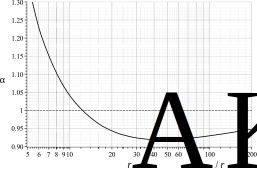
\includegraphics[width=9cm]{beta.pdf}\par
    \caption{Зависимость поправочного коэффициента $\beta$ от отношения радиусов
        электродов}
    \figmark{beta}
\end{figure}


\experiment 

Исследования проводятся на диоде с косвенным накалом (ток пропускается через 
расположенную вблизи катода \emph{нить накала}). Радиус его 
катода~$r_{К}$, анода~$r_{А}$, а также длина его активной области~$l$ 
указаны на установке. Отметим, что длина
активной области диода (участка катода, покрытого оксидным слоем, обеспечивающим
термоэмиссию электронов) обычно существенно меньше полной
высоты анода (примерно в два раза). Благодаря этому рабочая часть катода достаточно 
удалена от его торцов, и следовательно,
электрическое поле в активной части диода с хорошей точностью можно считать радиальным.

Схема экспериментальной установки изображена на рис.~\figref{Scheme}. Для
питания цепи накала и анода используются два регулируемых источника напряжения. 
Ток накала $I_{н}$ измеряется амперметром, включённым последовательно с
балластным сопротивлением $R$. Анодное напряжение~$U$ измеряется вольтметром, 
а анодный ток $I$~--- миллиамперметром.
В~работе предлагается измерять анодные токи и напряжения в широком диапазоне 
значений (перекрывающем примерно три порядка величины), 
поэтому вольтметр и миллиамперметр должны быть оснащены устройствами 
ручного или автоматического переключения диапазонов измерения.

\begin{figure}[h!]
    \centering
    \pic{9cm}{Chapter_3/3_2_2}
    \caption{Схема экспериментальной установки}
    \figmark{Scheme}
\end{figure}

\begin{lab:task}

\taskpreamble{В~работе предлагается исследовать вольт-амперные характеристики диода при
различных токах накала и по результатам
измерений определить удельный заряд электрона.}


    
\item Настройте измерительные приборы согласно прилагаемой к установке
инструкции.

\item Перед включением питания установите ручки регулировки источников
в минимальное положение.

\item Установите минимальный ток накала диода~$I_\text{н}$, 
и минимальное значение анодного напряжения~$V_{A}$, 
указанные в инструкции. Дайте лампе прогреться в течение 5--10 минут.

\item Проведите подробные измерения вольт-амперных характеристик диода 
$I(U)$ во всём допустимом диапазоне изменения напряжений  (см. инструкцию
к установке). 

Всего должно быть измерено не менее 25--30 точек, 
не менее чем по 8--10 на каждый диапазон изменения напряжений. 
Как правило, рекомендуется провести и измерения в диапазоне от 0,5 до 50~В, 
при этом для малых напряжений (до 5~В) измерения рекомендуется производить 
с шагом 0,5~В, для средних (до 15~В)~--- с шагом 1~В и 
для более высоких~--- с шагом 5~В.

\item Повторите измерения вольт-амперных характеристик 
еще при 2--3 рекомендованных значениях токах накала.

\tasksection{Обработка результатов}

\item По результатам проведенных измерений постройте 
вольт-амперные характеристики диода 
в двойном логарифмическом масштабе
$\log I (\log U)$
для каждого тока накала. По графикам определите участки, на которых
выполняется <<закон 3/2>>.

\item Используя данные, соответствующие участкам применимости
<<закона 3/2>>, постройте для каждого тока накала вольт-амперные 
характеристики в координатах $I(U^{3/2})$. 
Убедитесь в том, что зависимость имеет линейный характер. 

\item Найдите наклоны прямолинейных участков зависимости
$I(U^{3/2})$. Используя формулы \eqref{UI_inf}, \eqref{3.2.8}, 
определите удельный заряд электрона~$e/m$.

\item Оцените погрешность результата и сравните его с табличным.

\end{lab:task}


\begin{lab:questions}
    
    \item Каковы условия применимости <<закона 3/2>> для вакуумного диода?
    Почему закон неприменим при малых и больших напряжениях?
    
    \item Изобразите качественно зависимость тока диода от напряжения
    во всём диапазоне положительных напряжений $U_{А}>0$ на аноде.
    
	\item Нарисуйте качественные графики распределения потенциала $\varphi(r)$ 
    между катодом и анодом: а)~в режиме объёмного заряда;
б)~в режиме насыщения тока диода. Объясните эти зависимости.

    \item Как выглядит вольт-амперная характеристика диода при отрицательных
    напряжениях на аноде, $U_{А}<0$?

	\item Как влияет ток накала катода на ток диода при неизменном напряжении
на аноде? Приводит ли это к погрешности измерения~$e/m$?

    \item Получите уравнение \eqref{3.2.1} из интегральной формы теоремы Гаусса
    для электрического поля.
    
    \item Оцените, при каком токе через диод нельзя пренебрегать
    действием магнитного поля этого тока на движение электронов.

\end{lab:questions}

\begin{lab:literature}
    \item \Kirichenko~--- \S~2.4.
	\item \SivuhinIII~--- \S\S~100--102.
	\item \Kalashnikov~--- \S~157.
\end{lab:literature}


\lab{Опыт Милликена.}

\aim{измерение элементарного заряда методом масляных капель.}

\equip{плоский конденсатор в защитном кожухе, осветитель, измерительный
микроскоп, электростатический вольтметр,
электронный секундомер, переключатель напряжения, пульверизатор с маслом.}


Идея опыта очень проста. Если элементарный заряд действительно существует, то
заряд~$q$ любого тела может принимать
только дискретную последовательность значений:
\begin{equation}
	q=0,\,\pm e,\,\pm 2e,\,\pm 3e,\,\ldots\pm ne,\,\ldots,
	\eqmark{3.3.1}
\end{equation}
где~$e$~--- элементарный заряд. В предлагаемом опыте измеряется заряд небольших
капелек масла, несущих всего несколько элементарных зарядов. Сравнивая между
собой заряды капель, можно убедиться, что все они по модулю кратны одному и тому
же числу, которое равно, очевидно, элементарному заряду.

Для измерения заряда капель будем исследовать их движение в вертикальном
электрическом поле.

Движение заряженной капли в электрическом поле зависит как от электрических сил,
так и от массы капли. Масса капли может быть определена по скорости её падения в
отсутствие поля.

Рассмотрим свободное падение капли. Уравнение её движения при падении имеет вид
\begin{equation}
	m\frac{dv}{dt}=mg-F_\text{тр},
	\eqmark{3.3.2}
\end{equation}
где~$m$~--- масса капли, $v$ --- её скорость, $g$~--- ускорение свободного
падения, а~$F_\text{тр}$~--- сила вязкого трения капли в воздухе, которая для
сферической капли определяется формулой Стокса:
\begin{equation}
	F_\text{тр}=6\pi\eta rv=kv.
	\eqmark{3.3.3}
\end{equation}

Здесь~$r$~--- радиус капли, $\eta$~--- коэффициент вязкости воздуха, $k=6\pi\eta
r$. Подставляя \eqref{3.3.3} в \eqref{3.3.2}, получим
\begin{equation}
	m\frac{dv}{dt}=mg -kv.
	\eqmark{3.3.4}
\end{equation}

Можно убедиться, что при нулевой начальной скорости решение этого уравнения
имеет вид
\begin{equation}
	v=\frac{mg }{k}\left(1-e^{-kt/m}\right).
	\eqmark{3.3.5}
\end{equation}

Установившееся значение скорости равно
\begin{equation}
	v_\text{уст}=\frac{mg }{k}=\frac{\frac 43 \pi\rho r^3g }{6\pi\eta
r}=\frac29\frac{\rho}{\eta}g r^2,
	\eqmark{3.3.6}
\end{equation}
где $\rho$~--- плотность масла. Заметим, что \eqref{3.3.6} может быть немедленно
получено из \eqref{3.3.4}, если положить $dv/dt=0$.

Как следует из \eqref{3.3.5}, установление скорости происходит с постоянной
времени
\begin{equation}
	\tau=\frac{m}{k}=\frac 29 \frac{\rho}{\eta}r^2.
	\eqmark{3.3.7}
\end{equation}
Время установления скорости, таким образом, быстро падает с уменьшением радиуса
капли~$r$. Для мелких капель оно столь мало, что движение капли всегда можно
считать равномерным. Выражение \eqref{3.3.6} в этом случае позволяет определить
радиус капли, зная скорость её падения. Обозначая через~$h$ путь, пройденный
каплей за время~$t_0$, найдём
\begin{equation}
	r=\sqrt{\frac{9\eta h}{2\rho g t_0}}.
	\eqmark{3.3.8}
\end{equation}

Рассмотрим теперь движение капли при наличии электрического поля плоского
конденсатора, пластины которого расположены горизонтально. Напряжённость поля
$E$ в конденсаторе равна
\begin{equation}
	E=\frac{V}{l},
	\eqmark{3.3.9}
\end{equation}
где~$l$~--- расстояние между пластинами, $V$~--- разность потенциалов между
ними.

Нас будет интересовать случай, когда под действием электрического поля капля
поднимается. Уравнение движения при этом примет вид
\begin{equation}
	m\frac{dv}{dt}=\frac{qV}{l}-mg -kv,
	\eqmark{3.3.10}
\end{equation}
где~$q$~--- заряд капли. Появление в правой части постоянного слагаемого не
изменяет постоянной времени~$\tau$. Для
определения установившейся скорости мы можем снова положить левую часть
\eqref{3.3.10} равной нулю.

Измерим время~$t$ подъёма капли на начальную высоту. Используя равенства
\eqref{3.3.4}, \eqref{3.3.8} и \eqref{3.3.10}, найдём, что заряд капли равен
\begin{equation}
	q=9\pi\sqrt{\frac{2\eta^3 h^3}{g \rho}}\cdot\frac{l(t_0+t)}{Vt_0^{3/2} t}.
	\eqmark{3.3.11}
\end{equation}

Вывод формулы \eqref{3.3.11} предоставляем читателю.

\experiment Схема установки представлена на рис.~\figref{Scheme}. Масло
разбрызгивается пульверизатором. Капли масла попадают в конденсатор~$C$ через
небольшое отверстие в верхней пластине. При этом часть из них вследствие трения
о воздух приобретает случайный по абсолютной величине и знаку электрический
заряд.

Напряжение на пластины подаётся с регулируемого выпрямителя и измеряется
вольтметром~$V$. Ключ~$K$ позволяет менять направление поля в конденсаторе,
чтобы можно было работать  как с отрицательно, так и с положительно заряженными
каплями. При размыкании ключа~$K$ конденсатор разряжается через дополнительное
сопротивление $R\approx 10$~МОм.
\begin{figure}[h!]
	\pic{0.9\textwidth}{Chapter_3/3_3_1}
	\caption{Схема экспериментальной установки для измерения заряда электрона}
	\figmark{Scheme}
\end{figure}
Время отсчитывается по электронному секундомеру.

Естественно, что слабые электрические силы, действующие на каплю, несущую всего
один или несколько электронных зарядов, способны существенно изменить её
движение только в том случае, если сама она очень мала. Опыт производится
поэтому с мелкими каплями, наблюдение за которыми возможно только с помощью
микроскопа.

В фокальной плоскости окуляра измерительного микроскопа~$M$ виден ряд
горизонтальных линий, расстояние между которыми было предварительно определено с
помощью объектного микрометра. Для облегчения процесса измерений микроскоп может
снабжаться камерой с выводом изображения на дисплей ПК. Наблюдая за перемещением
капли между линиями, нетрудно определить путь, пройденный каплей. Время~$t_0$
свободного падения капли от одной выбранной линии до другой и время~$t$ её
обратного подъёма, происходящего под действием сил электрического поля,
измеряется электронным секундомером.

Из постановки опыта очевидно, что дискретность заряда может быть обнаружена лишь
в том случае, если ошибка~$\delta q$ в измерении заряда капли существенно меньше
абсолютной величины заряда электрона~$e$. Допустимая относительная ошибка опыта
$\delta q/q$ должна быть поэтому много меньше $e/q=1/n$, где~$n$~--- заряд
капли, выраженный в числе зарядов электрона. Этому условию тем легче
удовлетворить, чем меньше число~$n$. В нашем случае трудно определить~$q$ с
точностью лучше 5\%. Заряд капли должен поэтому быть существенно меньше 20
зарядов электрона~--- лучше всего, если он не превосходит пяти электронных
зарядов.

Из всех величин, входящих в формулу \eqref{3.3.11}, на опыте измеряются только
$t_0$, $t$, и~$V$. От точности определения этих величин зависит в основном
ошибка измерения~$q$. Из формулы \eqref{3.3.11} можно найти
\begin{equation}
	\frac{\sigma_q}{q}=\sqrt{\frac{\sigma^2_V}{V^2}+\frac{\sigma^2_t
t_0^2}{t^2(t_0+t)^2}+
	\frac{\sigma^2_{t_0}}{4t^2_0}\left(\frac{3t+t_0} {t+t_0}\right)^2}.
	\eqmark{3.3.12}
\end{equation}

При $t\approx t_0$ эта формула приобретает вид
\begin{equation}
	\frac{\sigma_q}{q}=\sqrt{\frac{\sigma^2_V}{V^2}+ \frac{\sigma^2_t}{4t^2_0}+
\frac{\sigma^2_{t_0}}{t^2_0}}.
	\eqmark{3.3.13}
\end{equation}

В условиях нашей работы наибольшее влияние на точность эксперимента оказывают
два последних стоящих под корнем члена. Ошибка измерения времени~$t_0$ и~$t$ при
визуальном наблюдении капель не может быть сделана меньше 0,1 -- 0,2 секунды.
Погрешность в измерении~$q$ будет поэтому тем меньше, чем большие значения
принимают~$t_0$ и~$t$. Для увеличения~$t_0$ и~$t$ можно было бы увеличить
расстояние, проходимое каплями, но это сильно усложнило бы экспериментальную
установку. Удобнее идти в другом направлении~--- работать с медленно движущимися
каплями, т.е. с каплями малого веса. Время падения~$t_0$ таких капель достаточно
велико. Чтобы время подъёма~$t$ было также достаточно большим, нужно
использовать не очень большие разности потенциалов~$V$.

Заметим, что выбор слишком маленьких капель приводит к снижению точности
измерений. Броуновское движение малых капель оказывает существенное влияние на
их движение и способно заметно исказить картину их падения и подъёма. Маленькие
капли могут испаряться, так что их размеры во время наблюдения могут
уменьшаться. При малых скоростях движения делаются особенно опасными
конвекционные потоки воздуха, которые возникают при неоднородном нагреве
установки (происходящем, например, от осветителя камеры). Практически в наших
условиях удобно выбирать $t_0\approx t\approx 10$ -- 30 секунд.

Для капель очень малого размера формула Стокса не вполне применима.
Использование формулы Стокса без поправок, впрочем, в наших условиях приводит к
искажению значений~$q$ и~$e$ не более чем на 10\% и почти не мешает обнаружению
дискретности электрического заряда. Мы рекомендуем поэтому не вводить в формулу
никаких поправок.

\begin{lab:task}

В работе предлагается по измерениям времени свободного падения заряженных капель
и времени их подъёма в электрическом поле определить заряд электрона.

\begin{enumerate}

\item{Перед началом работы оцените с помощью формулы \eqref{3.3.11} величину
напряжения~$V$, которое нужно для подъёма капель, несущих от 1 до 5 зарядов
электрона на высоту $h=1$~мм, задав $t_0\approx t=20$~с. Если для подъёма капель
потребуются меньшие напряжения, то соответствующие капли слишком сильно заряжены
и для эксперимента непригодны.

При вычислениях потребуются значения некоторых величин: расстояние между
пластинами $l=0,725$~см; плотность масла
$\rho=0,898$~г/см$^3$; коэффициент внутреннего трения воздуха $\eta=1,83\cdot
10^{-4}$~Пуаз~(СГС) или $1,83\cdot 10^{-5}$~Па$\cdot$с (СИ).}

\item{Включите осветитель. При этом падающий в камеру свет направлен под углом к
оси микроскопа и в объектив не попадает. Поле зрения микроскопа остаётся поэтому
тёмным. Капли масла рассеивают свет и кажутся светящимися точками на темном
фоне.

Не включая электрическое поле \important{слегка} надавите на грушу
пульверизатора  и наблюдайте за движением облачка масляных капель в поле зрения
микроскопа (изображение перевёрнуто).}

\item{Настройте окуляр микроскопа на резкое изображение делений окулярной шкалы.
Затем сфокусируйте объектив на появившиеся в рабочем пространстве капли.}

\item{Наблюдая за движением капель, следует выбирать капли, время падения
которых на $h=1$~мм лежит в пределах
10 -- 30 секунд, и научиться отличать их от более крупных, непригодных для
работы. Цена деления окулярной шкалы указана на установке.

В случае отсутствия в составе установки ПК с камерой регулировкой и коммутацией
напряжения занята одна рука наблюдателя. Вторая рука управляет секундомером.
Запись результатов измерений ($t_0$, $t$ и~$V$) ведёт второй экспериментатор.
Наблюдатель быстро устаёт, поэтому рекомендуется периодически меняться местами.
В случае наличия ПК указанные трудности отсутствуют, и работа может быть
выполнена одним экспериментатором.

Для уменьшения ошибок в определении~$t_0$ и~$t$ нужно для пуска и остановки
секундомера использовать один и тот же признак~--- всегда нажимать головку
секундомера либо в тот момент, когда капля скрывается за линией шкалы, либо,
наоборот, когда она появляется из-за линии. Рекомендуется следить за каплей, не
отрываясь от окуляра микроскопа, так как в противном случае легко её потерять из
виду и весь эксперимент придётся повторить.}

\item{В начале опыта следует позволить капелькам свободно падать \mbox{5 --
10}~секунд при выключенном электрическом поле для того, чтобы наиболее крупные
капли успели упасть на нижнюю пластину.

Из оставшихся в поле зрения капель выберите одну и произведите с ней серию
измерений, наблюдая её падение под действием силы тяжести и подъём под действием
электрического поля. Серия должна состоять из 5 -- 10 измерений~$t_0$ и такого
же числа измерений~$t$ для одной капли.}

\item{Необходимо проделать не менее 15 таких серий измерений (для 15~различных
капель), каждый раз регистрируя величину~$V$. При этом нужно иметь в виду, что
заряд капли может измениться во время наблюдений; в последнем случае для одной
капли получится несколько значений~$q$.

Изменение заряда капли может произойти при её подъёме в электрическом поле.
Вычисленное с помощью \eqref{3.3.11} значение заряда будет в этом случае
соответствовать некоторому среднему из величины заряда капли в начале и в конце
опыта. Соответствующий результат непригоден для обработки и только запутывает
опыт. Нужно поэтому стараться вовремя отбросить все случаи, когда перезарядка
капли произошла во время её подъёма. Это можно сделать, внимательно наблюдая за
движением капли и отбрасывая опыты, в которых капля изменила скорость подъёма во
время измерения.}

\item{Для оценки точности измерений <<подвесьте>> одну из капель в электрическом
поле. Определите соответствующее напряжение, отключите его  и измерьте время
падения капли на расстояние 2 -- 3-х делений шкалы. Поменяв полярность
напряжения, верните каплю на прежнее место и снова подвесьте её. Снова запишите
напряжение. Повторите  процедуру  для одной капли несколько раз  и на месте
оцените из этого опыта заряд капли по формуле \eqref{3.3.11}, полагая время
подъёма $t=\infty$. По разбросу результатов ($\Delta V$ и~$\Delta t$) оцените
точность измерения заряда этой капли.}

\end{enumerate}

\tasksection{Обработка результатов}

\begin{enumerate}

\item{Для всех исследованных капель рассчитайте значения~$q$, отложите их на
горизонтальной числовой оси и найдите для них общий наибольший делитель. Этот
наибольший делитель, вообще говоря, может оказаться равным~$e$, $2e$, $3e$ и
т.~д. Однако, чем больше значений~$q$ было измерено на опыте, тем меньше
вероятность получить в качестве делителя число, отличное от~$e$. Найденное
значение~$e$ приведите в системе единиц СИ и в системе СГС.}

\item{Оцените время релаксации $\tau=v_\text{уст}/g$ и расстояние~$s$, которое
прошла бы капля за это время с установившейся скоростью:
\begin{equation*}
	s=v_\text{уст}\tau=\frac{1}{g}\left(\frac{h}{t_0}\right)^2.
\end{equation*}}

\end{enumerate}

\end{lab:task}

\begin{lab:questions}

\item{Почему не следует выбирать капли слишком большого и слишком маленького
размера?}

\item{Какие напряжения соответствуют оптимальным условиям опыта? Приведите
расчёты.}

\item{Нарисуйте график зависимости скорости капли в поле силы тяжести от времени
и укажите на нём время и путь релаксации.}

\item{Зная параметры установки, оцените ёмкость конденсатора~$C$ и время его
разрядки через сопротивление~$R$ (площадь пластин ${\approx} 20$~см$^2$).}

\item{$^*$ Какие ещё способы измерения заряда электрона вам известны?}

\end{lab:questions}

\begin{lab:literature}

\item{ \emph{Сивухин Д.В.} Общий курс физики. Т.~III. Электричество. ---
М.:Физматлит, 2015. Гл.~V, \S~90.}

\item{ \emph{Калашников С.Г.} Электричество.~--- М.: Физматлит, 2003. Гл.~XVII,
\S~178.}

\end{lab:literature}

\lab{Эффект Холла в полупроводниках}

\aim{измерение подвижности и концентрации носителей заряда в полупроводниках.}

\equip{электромагнит с регулируемым источником питания; 
вольтметр; амперметр; миллиамперметр; милливеберметр или миллитесламетр;
источник питания (1,5~В), образцы легированного германия.}

Перед выполнением работы необходимо ознакомиться с основами
элементарной теории движения носителей заряда в~металлах и полупроводниках
(п. \ref{sec:halleffect} Введения к разделу).

В работе изучаются особенности проводимости полупроводников
в геометрии \emph{мостика Холла}.
Ток пропускается по плоской полупроводниковой пластинке, 
помещённой в перпендикулярное пластинке магнитное поле.
Измеряется разность потенциалов между краями пластинки в поперечном
к току направлении. По измерениям определяется \emph{константа Холла},
тип проводимости (\emph{электронный} или \emph{дырочный}) и на основе
соотношения \chaptereqref{HallConstant} вычисляется концентрация основных
носителей заряда.

\experiment
Электрическая схема установки для измерения ЭДС Холла представлена
на рис.~\figref{Scheme}. В зазоре электромагнита (рис.~\figref{Scheme}а) 
создаётся постоянное магнитное поле, величину которого можно менять с помощью 
регулятора источника питания электромагнита. Ток питания электромагнита 
измеряется амперметром А$_1$ (внешним, или встроенным в источник).
Направление тока в обмотках электромагнита меняется переключением
разъёма~К$_1$.

Градуировка электромагнита (связь тока с индукцией поля) проводится 
при помощи милливеберметра (его описание и правила работы 
с ним приведены на с.~\pageref{MWB}) или миллитесламетра на основе
датчика Холла.

\begin{figure}[h]
    \centering
	\pic{\textwidth}{Chapter_3/3_4_1}
	\caption{Схема установки для исследования эффекта Холла в~полупроводниках}
	\figmark{Scheme}
\end{figure}

Прямоугольный образец из легированного германия, смонтированный в специальном держателе
(рис.~\figref{Scheme}б), подключается к источнику питания ($\simeq 1,5$~В). При
замыкании ключа~К$_2$ вдоль длинной стороны образца течёт ток, величина которого
регулируется реостатом~$R_2$ и измеряется миллиамперметром~А$_2$.

В образце, помещённом в зазор электромагнита, между 
контактами~3 и~4 возникает разность потенциалов~$U_{34}$, 
которая измеряется с помощью вольтметра~V.

Контакты~3 и~4 вследствие неточности подпайки могут лежать не на одной
эквипотенциали. Тогда напряжение между ними связано не только с эффектом
Холла, но и с омическим падением напряжения вдоль пластинки. 
Исключить этот эффект можно, изменяя направление магнитного поля, 
пронизывающего образец. 
При обращении поля ЭДС Холла меняет знак, а омическое падение напряжения
остаётся неизменным. Поэтому ЭДС Холла~$U_{\perp}$ может быть определена
как половина алгебраической разности показаний вольтметра, полученных для двух
противоположных направлений магнитного поля в~зазоре:
$U_{\perp} = \frac12 (U_{34}^{(+)}-U_{34}^{(-)})$.

Альтернативно, можно исключить влияние омического падения напряжения, 
если при каждом значении тока через образец измерять напряжение
между точками~3 и~4 в отсутствие магнитного поля. При фиксированном токе через
образец это дополнительное к ЭДС Холла напряжение~$U_0$ остаётся неизменным. 
От него следует (с учётом знака) отсчитывать величину ЭДС Холла:
\begin{equation}
	U_{\perp} = U_{34} - U_0.
	\eqmark{3.4.1}
\end{equation}
При таком способе измерения нет необходимости проводить повторные измерения
с противоположным направлением магнитного поля.

По знаку $U_{\perp}$ можно определить характер проводимости~--- 
электронный или дырочный. Для этого необходимо знать направление тока 
в образце и направление магнитного поля.

Измерив ток~$I$ в образце и напряжение~$U_{35}$ между контактами~3 и~5 в
отсутствие магнитного поля, можно, зная
параметры образца, рассчитать проводимость материала образца по формуле
\begin{equation}
	\rho_0=\frac{U_{35}ah}{Il},
	\eqmark{3.4.2}
\end{equation}
где $l$~--- расстояние между контактами~3 и~5, $w$~--- ширина образца, $h$~---
его толщина.

\begin{lab:task}

\taskpreamble{В работе предлагается исследовать зависимость ЭДС Холла от величины магнитного
поля при различных значениях тока через образец для определения константы Холла;
определить знак носителей заряда и проводимость материала образца.}

\item Подготовьте приборы к работе согласно описанию на установке.

\item Проверьте работу цепи питания образца. Ток через образец не должен
превышать 1~мА.

\item Установите ручки регулировки источника питания электромагнита 
в минимальное положение и включите источник. 
Плавно изменяя ток магнита, определите диапазон его изменения.

\item Измерьте калибровочную кривую электромагнита~---
зависимость между индукцией~$B$ магнитного поля в его зазоре и 
током~$I_{М}$ через обмотки магнита.
Магнитное поле измеряется милливеберметром или миллитесламетром
(датчиком Холла). Калибровочная кривая должна содержать не менее
15 точек во всём диапазоне изменения токов.

В~случае использования милливеберметра измерьте зависимость 
магнитного потока~$\Phi$, пронизывающего пробную катушку, 
находящуюся в зазоре, от тока~$I_{М}$ ($\Phi=BSN$). 
Значение~$SN$ (произведение площади сечения контура катушки на
число витков в ней) указано на держателе катушки.

\item \label{p1} Вставьте образец в зазор \emph{выключенного} электромагнита 
и определите напряжение $U_0$ между холловскими
контактами~3 и~4 при минимальном токе через образец ($I\simeq 0,2$~мА). Это
напряжение~$U_0$ вызвано несовершенством контактов~3, 4 и при фиксированном токе
через образец остаётся неизменным. Значение~$U_0$ с учётом знака следует принять
за начало отсчёта напряжения.

\item \label{p2} Проведите измерение ЭДС Холла: снимите зависимость напряжения~$U_{34}$ 
от тока электромагнита~$I_{М}$ (6--8 точек) при фиксированном токе~$I$ 
через образец.

\item Повторите измерения пп. \ref{p1}, \ref{p2} при 6--8 токах $I$ через образец
(рекомендованные токи указаны в описании установки).  
Учтите, что при каждом новом токе $I$ величина~$U_0$ будет иметь 
своё значение.

\item При максимальном токе через образец проведите измерения $U_{34}(I_{M})$ 
при обратном направлении магнитного поля.

\item Определите знак носителей заряда в образце. Для этого необходимо знать
направление тока через образец, направление магнитного поля и знак ЭДС Холла.

Направление тока в образце показано знаками~<<$+$>> и~<<$-$>> на
рис.~\figref{Scheme}. Направление тока в обмотках электромагнита при 
установке разъёма~К$_1$ в положение~1 показано стрелкой на торце магнита.
Знак напряжения $U_{34}$ показан на дисплее цифрового вольтметра.

Зарисуйте в тетради образец. Укажите на рисунке направления тока, магнитного
поля и отклонение носителей. Определите характер проводимости образца
(дырочный или электронный)

\item Измерьте удельную проводимость образца. Для этого: 
удалите держатель с образцом из зазора электромагнита;
установите максимальный ток через образец, используемый в предыдущих измерениях;
и с помощью вольтметра измерьте падение напряжения между проводниками, 
подключёнными к точкам~3 и~5 образца.

\item Запишите характеристики приборов и параметры образца, указанные на держателе:
длину~$l$ (расстояние между точками~3 и~5), ширину~$a$, толщину~$h$.


\tasksection{Обработка результатов}

\item Постройте калибровочный график зависимости $B(I_{M})$. 
Используйте эту зависимость для дальнейшего пересчёта (интерполяции)
значений поля по измеренным токам $I_{М}$.


\item Рассчитайте ЭДС Холла по формуле \eqref{3.4.1} и постройте на одном листе
семейство характеристик $U_{\perp}(B)$ при разных значениях тока~$I$ через
образец. Убедитесь в линейности зависимостей и определите угловые 
коэффициенты $k=dU_{\perp}/dB$ полученных прямых.

\item Постройте график $k(I)$. Рассчитайте угловой коэффициент прямой 
и по формуле \chaptereqref{3.19} определите величину постоянной Холла~$R_{\rm H}$.

\item Рассчитайте концентрацию $n$ носителей тока в образце,
удельное сопротивление $\rho_0$ и удельную проводимость $\lambda_0$ материала.

\item Используя найденные значения концентрации~$n$ и удельной проводимости
$\lambda_0=1/\rho_0$, вычислите 
подвижность~$\mu$ носителей тока. Ответ представьте в общепринятых для этой величины 
внесистемных единицах $[\mu]=$~см$^2/(В\cdotс)$
(размерность напряжённости $[E]=$~B/см, скорости $[v]=$~см/с,
поэтому $[\mu]=[v/E]=$~см$^2/(В\cdot с)$).

\item Оцените погрешности и сравните результаты с табличными.

\end{lab:task}


\begin{lab:questions}

\item Какие вещества называют диэлектриками, проводниками, полупроводниками?
Чем объясняется различие их электрических свойств? Как зависит от температуры
проводимость металлов и полупроводников?

\item Дайте определение константы Холла. Как зависит константа Холла от
температуры у металлов и полупроводников?

\item Зависит ли результат измерения константы Холла от геометрии образца?

\item Зависит ли сопротивление образца от магнитного поля 
в условиях опыта?

\item Как устроен милливеберметр? Зависят ли его показания от сопротивления
измерительной катушки? Каким должно быть это сопротивление по сравнению с
сопротивлением катушки прибора?

\item По результатам измерений оцените частоту столкновений, длину пробега
и коэффициент диффузии носителей тока в образце.

\item Получите выражение константы Холла для материалов с~двумя типами
носителей. \emph{Указание}: воспользуйтесь условием равенства нулю поперечного тока.

\end{lab:questions}


\begin{lab:literature}
\item \SivuhinIII~--- \S\S~98, 100.
\item \textit{Парселл Э.} Электричество и магнетизм.~--- М.: Наука, 1983. Гл.~4,
\S\S~4--6; Гл.~6, \S~9
\end{lab:literature}


\lab{Эффект Холла в металлах}

\aim{измерение подвижности и концентрации носителей заряда в металлах.}

\equip{электромагнит с источником питания, источник постоянного тока,
микровольтметр, амперметры, милливеберметр или цифровой магнитометр, образцы из
меди, серебра и цинка.}

Перед выполнением работы необходимо ознакомиться с основами
элементарной теории движения носителей заряда в~металлах и полупроводниках
(п. \ref{sec:halleffect} Введения к разделу).

В работе изучаются особенности проводимости металлов
в геометрии \emph{мостика Холла}.
Ток пропускается по плоской металлической пластинке, 
помещённой в перпендикулярное пластинке магнитное поле,
и измеряется разность потенциалов между краями пластинки в поперечном
к току направлении. По измерениям определяется \emph{константа Холла},
тип проводимости (\emph{электронный} или \emph{дырочный}) и на основе
соотношения \chaptereqref{HallConstant} вычисляется концентрация основных
носителей заряда.

\experiment Электрическая схема установки для измерения ЭДС Холла представлена
на рис.~\figref{Scheme}.

\begin{figure}[h!]
	\pic{0.9\textwidth}{Chapter_3/3_5_1}
	\caption{Схема установки для исследования эффекта Холла в~металлах}
	\figmark{Scheme}
\end{figure}

В зазоре электромагнита (рис.~\figref{Scheme}а) создаётся постоянное магнитное
поле, величину которого можно менять с помощью источника питания электромагнита.
Разъём~$K_1$ позволяет менять направление тока в обмотках электромагнита. Ток
питания электромагнита измеряется амперметром~$A_1$.

Градуировка магнита проводится с помощью милливеберметра (его описание и правила
работы с ним приведены на с.~\pageref{MWB}) или цифрового магнитометра на основе
датчика Холла.

Металлические образцы в форме тонких пластинок, смонтированные в специальных
держателях, подключаются к блоку питания через разъём (рис.~\figref{Scheme}б).
Ток через образец регулируется реостатом~$R_2$ и измеряется амперметром~$A_2$.

Для измерений ЭДС Холла используется микровольтметр $\text{Ф}116/1$, в котором
высокая чувствительность по напряжению сочетается с малой величиной тока,
потребляемого измерительной схемой: минимальный предел измерения напряжения
составляет 1 мкВ, а потребляемый ток~--- всего $10^{-8}$~А.

В образце с током, помещённом в зазор электромагнита, между контактами~2 и~4
возникает холловская разность потенциалов, которая измеряется с помощью
микровольтметра, если переключатель~$K_3$ подключён к точке 2 образца. При
подключении~$K_3$ к точке~3 микровольтметр измеряет омическое падение напряжения
$U_{34}$, вызванное основным током через образец. При нейтральном положении
ключа входная цепь микровольтметра разомкнута.

Ключ~$K_2$ позволяет менять полярность напряжения, поступающего на вход
микровольтметра.

Иногда контакты~2 и~4 вследствие неточности подпайки не лежат на одной
эквипотенциали, и тогда напряжение между ними связано не только с эффектом
Холла, но и с омическим падением напряжения, вызванным протеканием основного
тока через образец. Измеряемая разность потенциалов при одном направлении
магнитного поля равна сумме ЭДС Холла и омического падения напряжения, а при
другом~--- их разности. В этом случае ЭДС Холла~$V_{xy}$ может быть определена
как половина алгебраической разности показаний вольтметра, полученных для двух
противоположных направлений магнитного поля в зазоре.

Можно исключить влияние омического падения напряжения иначе, если при каждом
токе через образец измерять
напряжение~$U_0$ между точками~2 и~4 в отсутствие магнитного поля. При
фиксированном токе через образец это
дополнительное к ЭДС Холла напряжение остаётся неизменным. От него следует (с
учётом знака) отсчитывать величину ЭДС Холла:
\begin{equation}
	V_{xy}=U_{24}\pm U_0.
	\eqmark{3.5.1}
\end{equation}

При таком способе измерения нет необходимости проводить повторные измерения с
противоположным направлением магнитного поля.

По знаку~$V_{xy}$ можно определить характер проводимости~--- электронный или
дырочный. Для этого необходимо знать направление тока в образце и направление
магнитного поля.

Измерив ток~$I$ в образце и напряжение~$U_{34}$ между контактами~3 и~4 в
отсутствие магнитного поля, можно, зная параметры образца, рассчитать удельное
сопотивление материала образца по очевидной формуле:
\begin{equation}
	\rho_0=\frac{U_{34}wh}{Il},
	\eqmark{3.5.2}
\end{equation}
где $l$~--- расстояние между контактами~3 и~4, $w$~--- ширина образца, $h$~---
его толщина.

\labtask

В работе предлагается исследовать зависимость ЭДС~Холла от величины магнитного
поля при различных токах через образец для определения константы Холла;
определить знак носителей заряда и проводимость различных металлических
образцов.

\begin{lab:task}

\item{Подготовьте приборы к работе.}

\item{ Проверьте работу цепи питания образца. Для этого подключите к разъёму
блока управления один из образцов~--- медный или серебряный. Убедитесь, что ток
через образец можно изменять в указанных в описании пределах.}
\item{ Проверьте работу цепи магнита. Установите разъём~$K_1$ в положение~I и
определите диапазон изменения тока через электромагнит.}
\item{ Прокалибруйте электромагнит. Для этого вставьте в зазор электромагнита
пробную катушку милливеберметра и исследуйте зависимость магнитного потока
$\Phi$, пронизывающего пробную катушку, от тока~$I_M$ через обмотки магнита
($\Phi=BSN$). Значение~$SN$ (площадь сечения пробной катушки на число витков в
ней) указано на держателе катушки.

Проведите измерения магнитного потока для 6 -- 8 значений тока через
электромагнит.}

\item{ Проведите измерение ЭДС Холла. Для этого вставьте образец в зазор
выключенного электромагнита и определите напряжение~$U_0$ между холловскими
контактами~2 и~4 при минимальном токе через образец. Это напряжение~$U_0$
вызвано несовершенством контактов~2, 4 и при фиксированном токе через образец
остаётся неизменным. Значение~$U_0$ с учётом знака следует принять за нулевое.

Включите электромагнит и снимите зависимость напряжения~$U_{24}$ от тока~$I_M$
через обмотки магнита при фиксированном токе через образец. Измерения следует
проводить при \important{медленном} увеличении магнитного поля. Резкие изменения
магнитного поля наводят ЭДС индукции в подводящих проводах и вызывают большие
отклонения стрелки микровольтметра.

Повторите измерения $U=f(I_{M})$ при постоянном токе через образец для 5 -- 6
его значений в интервале, указанном в описании конкретной установки. При каждом
новом значении тока через образец величина~$U_0$ будет иметь своё значение.

При максимальном токе через образец проведите измерения $U=f(I_{M})$ при другом
направлении магнитного поля.

Для образца из цинка снимите зависимость $U=f(I_{M})$ при одном значении тока
через образец.}

\item{Определите знак носителей в образце. Для этого необходимо знать
направление тока через образец, направление магнитного поля и знак ЭДС Холла.
Направление тока в образце показано знаками~<<$+$>> и~<<$-$>> на
рис.~\figref{Scheme}. Направление тока в обмотках электромагнита при установке
разъёма~$K_1$ в положение~I показано стрелкой на торце магнита.

Напомним, что знак потенциала, соответствующий точкам~2 или~4, можно определить
по рис.~\figref{Scheme}.

Зарисуйте в тетради образец. Укажите на рисунке направление тока, магнитного
поля (положение разъёма~$K_1$) и знак
потенциала, соответствующий клемме~4 (положение ключа~$K_2$ при отклонении
стрелки вольтметра вправо).

Определите знак носителей заряда для каждого из двух образцов.}
\item{Определите удельную сопротивление образца. Для этого удалите держатель с
образцом из зазора. Переключите микровольтметр (в случае необходимости) в режим
измерения милливольтовых напряжений. Ключ~$K_3$ поставьте в положение $U_{34}$.
При токе через образец порядка максимального значения в предыдущих измерениях
измерьте падение напряжения между контактами~3 и~4 для каждого из двух
образцов.}

\item{ Запишите характеристики приборов и параметры образцов $l$, $w$, $h$
(длину, ширину и толщину), указанные на держателях.}

\tasksection{Обработка результатов}

\item{Рассчитайте индукцию магнитного поля~$B$ для каждого значения тока и
постройте график зависимости $B=f(I_{M})$.}

\item{Рассчитайте ЭДС Холла по формуле \eqref{3.5.1} и постройте на одном листе
семейство характеристик $V_{xy}=f(B)$ при разных значениях тока~$I$ через
образец (для меди или серебра). Определите угловые коэффициенты $k(I)=\Delta
V_{xy}/\Delta B$ полученных прямых.}

\item{ Постройте график $k=f(I)$. Рассчитайте угловой коэффициент прямой и по
формуле \chaptereqref{3.19} определите величину постоянной Холла~$R_X$.

Для цинка изобразите на графике зависимость $V_{xy}=f(B)$ и по наклону прямой
рассчитайте постоянную Холла.

Для обоих образцов рассчитайте концентрацию~$n$ носителей тока по формуле
\chaptereqref{HallConstant}.

Оцените погрешности и сравните результаты с табличными.}

\item{ Рассчитайте удельное сопротивление~$\rho_0$ материала образцов по формуле
\eqref{3.5.2}.

Используя найденные значения концентрации~$n$ и проводимости~$\rho_0$, с помощью
формулы \chaptereqref{UdSoprot} рассчитайте подвижность $b$ носителей тока
в~общепринятых для этой величины внесистемных единицах: размерность
напряжённости электрического поля $[E] = [U/L]=\text{В/см}$, размерность
скорости $[v]=\text{см/с}$, поэтому размерность подвижности
$[b]=$см$^2$/(\text{В}$\cdot$\text{с}).

Оцените погрешности и сравните результаты с табличными.
}

\end{lab:task}


\begin{lab:questions}

\item{ Какие вещества называют диэлектриками, проводниками, полупроводниками?
Чем объясняется различие их электрических свойств? Как зависит от температуры
проводимость металлов и полупроводников?}

\item{ Дайте определение константы Холла. Как зависит константа Холла от
температуры у металлов и полупроводников?}

\item{ Зависит ли результат измерения константы Холла от геометрии образца?}

\item{ Как устроен милливеберметр? Зависят ли его показания от сопротивления
измерительной катушки? Каким должно быть это сопротивление по сравнению с
сопротивлением рамки прибора: большим или маленьким?}

\end{lab:questions}

\begin{lab:literature}

\item{ \emph{Сивухин Д.В.} Общий курс физики. Т.~III. Электричество~--- М.:
Наука, 1983. \S\S~98, 100.}

\item{ \emph{Парселл Э.} Электричество и магнетизм.~--- М.: Наука, 1983. Гл.~4,
\S\S~4--6; Гл.~6, \S~9 (Берклеевский курс физики. Т.~II).}
\end{lab:literature}

\lab{Влияние магнитного поля на проводимость полупроводников}

\aim{измерение зависимости сопротивления 
    полупроводниковых образцов различной формы от магнитного поля.}

\equip{электромагнит, милливеберметр или миллитесламетр (на основе датчика
Холла), вольтметр, амперметр, миллиамперметр, реостат, образцы
монокристаллического антимонида индия (InSb) $n$-типа.}

Перед выполнением работы необходимо ознакомиться с основами
элементарной теории движения носителей заряда в~металлах и полупроводниках
(п. \ref{sec:halleffect} Введения к разделу).

В работе изучается зависимость проводимости полупроводников от магнитного поля
в геометрии \emph{диска Корбино}.
По диску, помещенному в перпендикулярное ему магнитное поле, пропускается
ток в радиальном направлении. Магнитное поле искривляет линии 
тока, благодаря чему эффективное сопротивление образца возрастает
(эффект \emph{геометрического магнетосопротивления}). По результатам
измерений зависимости сопротивления от магнитного поля 
могут быть вычислены подвижность и концентрация носителей тока в образце.

\experiment
Схема установки для исследования магнетосопротивления
полупроводников и геометрического резистивного эффекта представлена на
рис.~\figref{Scheme}.

\begin{figure}[h!]
    \centering
    \pic{0.9\textwidth}{Chapter_3/3_6_1}
    \caption{Схема установки для~исследования влияния магнитного~поля
        на~проводимость полупроводников}
    \figmark{Scheme}
\end{figure}

В зазоре электромагнита (рис.~\figref{Scheme}а) создаётся постоянное магнитное
поле, величину которого можно менять с помощью источника питания электромагнита.
Ток электромагнита измеряется амперметром А$_1$ (отдельным или встроенным в источник).
Магнитная индукция в зазоре измеряется при помощи милливеберметра (его описание
и правила работы с ним приведены на с.~\pageref{MWB}) или 
миллитесламетра на основе датчика Холла.

Образец в форме кольца (диск Корбино) или пластинки, смонтированный в
специальном держателе, подключается к источнику постоянного напряжения 5~В. При
замыкании ключа~К$_2$ сквозь образец течёт ток, величина которого измеряется
миллиамперметром~А$_2$ и регулируется реостатом~$R_2$. Балластное сопротивление~$R_0$
ограничивает ток через образец. Измеряемое напряжение подаётся на вход
вольтметра~V.

\labtask


В работе предлагается при постоянном токе через образец исследовать зависимость
напряжения на образце от величины магнитного поля и от ориентации образца в
магнитном поле; по результатам измерений рассчитать подвижность электронов,
удельное сопротивление материала образца и концентрацию электронов.

\begin{lab:task}

\item Подготовьте приборы к работе согласно описанию на установке.

\item Концы от точек~3 и~4 разъёма подсоедините к клеммам вольтметра.
Присоедините диск Корбино через разъём к цепи питания. Определите
диапазон изменения силы тока через образец.

\item Установите ручки регулировки источника питания электромагнита 
в минимальное положение и включите источник. 
Плавно меняя ток магнита, определите диапазон его изменения.

\item Измерьте калибровочную кривую электромагнита~---
зависимость между индукцией~$B$ магнитного поля в его зазоре и 
током~$I_{М}$ через обмотки магнита.
Магнитное поле измеряется милливеберметром или миллитесламетром
(датчиком Холла). Калибровочная кривая должна содержать не менее
15 точек во всём диапазоне изменения токов.

В~случае использования милливеберметра измерьте зависимость 
магнитного потока~$\Phi$, пронизывающего пробную катушку, 
находящуюся в зазоре, от тока~$I_{М}$ ($\Phi=BSN$). 
Значение~$SN$ (произведение площади сечения контура катушки на
число витков в ней) указано на держателе катушки.

\item \label{p1} Вставьте образец в зазор \emph{выключенного} электромагнита 
и измерьте падение напряжения $U_0$ в образце при некотором токе,
рекомендованном в описании ($I_0\sim 25$~мА). 

\item \label{p2} Включите электромагнит и измерьте зависимость напряжения~$U$ 
на образце от тока через обмотки магнита~$I_M$ при фиксированном токе
через образец~$I_0$.

\item Проверьте, что результат измерения не зависит от направления магнитного
поля.

%\item Повторите измерения пп. \ref{p1}, \ref{p2} 
%для 3--4 других значений тока $I_0$ через образец.

\item Вместо диска Корбино подключите к измерительной цепи образец, имеющий
форму пластинки. Поместите образец в зазор выключенного электромагнита и
измерьте падение напряжения~$U_0$ на образце при токе через образец $10$~мА.

\item Включите электромагнит и снимите зависимость напряжения~$U$ на образце от
тока через магнит при постоянном токе $I=10$~мА. При измерениях длинная сторона
образца должна быть направлена поперёк поля, а средняя (ширина) в~одной серии
опытов располагается вдоль, а в другой~--- поперёк поля.

\item Запишите геометрические размеры образцов и характеристики приборов.

\tasksection{Обработка результатов}

\item Постройте калибровочный график зависимости $B(I_{M})$. 
    Используйте эту зависимость для дальнейшего пересчёта (интерполяции)
    значений поля по измеренным токам $I_{М}$.

\item Для всех серий измерений постройте графики, отложив по оси абсцисс
величину~$B^2$, а по оси ординат~--- величину $(U-U_0)/U_0$. Какие выводы
можно сделать на основании построенных зависимостей?

\item По наклону прямолинейного участка графика для диска Корбино рассчитайте
с помощью формулы \chaptereqref{MagnetoSoprot} подвижность носителей.

\item Определите сопротивление диска $R_0$ в отсутствие магнитного поля.
По геометрическим размерам образца рассчитайте удельное сопротивление~$\rho_0$ 
и удельную проводимость $\lambda_0=1/\rho_0$ материала образца.

\item С помощью формулы \chaptereqref{3.26} найдите концентрацию носителей
тока.

\item Оцените погрешности и сравните результаты с табличными.

\end{lab:task}


\begin{lab:questions}

\item Какие вещества называют диэлектриками, проводниками, полупроводниками?
Чем объясняется различие их электрических свойств? Как зависит от температуры
проводимость металлов и полупроводников?

\item В чем причина зависимости сопротивления образца от магнитного
поля в геометрии диска Корбино?

\item Зависит ли эффект магнетосопротивления от геометрии образца? 
В каких случаях эффект магнетосопротивления может проявиться
при протекании тока по плоской пластинке?

\item Как устроен милливеберметр? Зависят ли его показания от сопротивления
измерительной катушки? Каким должно быть это сопротивление по сравнению с
сопротивлением рамки прибора: большим или маленьким?

\item По результатам измерений оцените частоту столкновений,
длину пробега и коэффициент диффузии носителей тока в исследуемом материале.

\item Получите выражение для сопротивления пластинки, изготовленной
из материала с~двумя типами носителей. 
Для простоты можно ограничиться случаем $\mu_e \gg \mu_h$.

\end{lab:questions}


\begin{lab:literature}
\item \SivuhinIII~--- \S\S~98, 100.
\item \textit{Парселл Э.} Электричество и магнетизм.~--- М.: Наука, 1983. Гл.~4,
\S\S~4--6; Гл.~6, \S~9.
\end{lab:literature}



\cleardoublepage
\chapter{Магнитные свойства вещества}

Известно, что вещество может обладать как собственной намагниченностью, так
и изменять свою намагниченность при помещении во внешнее магнитное поле.
Источниками магнитного поля в среде могут служить орбитальное движение электронов
в молекулах и атомах, а также собственное вращение (спин) электронов и ядер.
Не вдаваясь в детальное описание микроскопических свойств среды, можно считать,
что каждый элемент объёма среды может являться элементарным источником
магнитного поля --- \important{магнитным диполем}. Для описания усреднённых
(макроскопических) свойств среды используют
\important{вектор намагниченности} $\vec{M}$, равный
\emph{магнитному моменту единичного объёма вещества} (объёмная плотность магнитного момента).

Среднее значение магнитного поля в некоторой точки среды есть вектор
$\vec{B}$, называемый (по историческим причинам) \important{индукцией поля}.
Помимо этого, принято вводить вспомогательный вектор $\vec{H}$
(\important{напря\-жённость поля}), определяемый из соотношения
\begin{equation}
    \eqmark{fieldB}
    \vec{B} = \mu_0(\vec{H} + \vec{M}).
\end{equation}

В простейшем практически важном случае намагниченность $\vec{M}$ в каждой
точке среды прямо пропорциональна вектору напряжённости магнитного
поля~$\vec{H}$ в этой же точке:
\begin{equation}
    \eqmark{magnetization}
    \vec{M} = \chi\vec{H}.
\end{equation}
Коэффициент $\chi$ называют \important{магнитной восприимчивостью} среды.
Вещества, для которых закон \eqref{magnetization} выполняется
с хорошей точностью, называют \important{парамагнетиками} ($\chi > 0$) и
\important{диамагнетиками} ($\chi < 0$).
В~парамагнетиках элементарные диполи
ориентированы в основном по приложенному полю,
а в диамагнетиках --- против него.

Если закон \eqref{magnetization} применим,
то можно записать
\begin{equation}
    \vec{B} = \mu\mu_0 \vec{H},\qquad \text{где }\mu = 1 + \chi
\end{equation}
--- \important{магнитная проницаемость} вещества%
\footnote{В системе СГС имеют место соотношения
    $\vec{B}=\vec{H}+4\pi\vec{M}=\mu\vec{H}$, $\mu = 1 + 4\pi \chi$.}.

Отметим. что в общем случае зависимость $\vec{M}$ от $\vec{H}$ в среде может
не только быть нелинейной, но и зависеть от ``предыстории'' образца ---
значения полей в предыдущие моменты времени
(явление \important{гистерезиса} в ферромагнетиках).




\labsection{Диамагнетизм}

Полноценное рассмотрение движения электрона в атоме возможно только с
использованием квантовой механики. В этом разделе мы ограничимся рассмотрением
упрощённых полуклассических моделей, которые, тем не менее,
наглядны и дают правильные по порядку величины результаты.

Рассмотрим электрон в атоме, находящийся в состоянии с нулевым
орбитальным моментом импульса $L=0$ ($s$-состояние). Соответствующий магнитный
момент также равен нулю $\mu_L = 0$ (собственный, т.\,е. спиновый,
момент электрона рассматривать не будем).
С классической точки зрения такое состояние можно представить как симметрично
``размазанное'' облако заряда вокруг ядра.
% Пусть средний радиус облака равен $a$, масса электрона $m_e$, заряд $-e$.

Плавно (квазистатически) включим внешнее однородное магнитное поле $\vec{B}$.
Под действием вихревого электрического поля, возникающего из-за наличия
переменного магнитного поля, электронное облако придёт во вращение.
Согласно закону электромагнитной индукции, величина этого поля на расстоянии $r$ от оси системы определяется соотношением
\[
2\pi r E = - \pi r^2 \frac{dB}{dt}\qquad \to \qquad E = - \frac12 r\frac{dB}{dt}.
\]
Запишем уравнение моментов для точечного электрона,
находящегося на ``орбите'' радиуса $r$:
\[
m_e r^2 \frac{d\omega}{dt} = - e r E = \frac12 er^2\frac{dB}{dt}.
\]
Интегрируя по времени, находим, что независимо от расстояния $r$ электрон при
включении поля $B$ приобретает угловую скорость вращения
\begin{equation}
    \eqmark{Larmor-Omega}
    \omega_L = \frac{eB}{2m_e c}.
\end{equation}
Величину $\omega_L$ называют \important{ларморовской} частотой.

При вращении с ларморовской частотой электрон создаёт магнитное поле,
равное полю витка с током $I_L = e \frac{\omega_L}{2\pi}$.
Этот ток в свою очередь создаёт магнитный момент
\begin{equation*}
  \Delta\mu_L = \Delta I \cdot S = - \frac{e^2 S}{4\pi m_e}B,
\end{equation*}
где $S$~--- площадь эквивалентного витка.
Примем для оценки $S\sim \pi a^2$, где $a$ --- среднее расстояние электронов до ядра
(аккуратный учёт сферической симметрии электронного облака
даёт поправочный множитель $2/3$: $S=\frac23 \pi \left<r^2\right>$).
Тогда, для атома, содержащего $Z$ электронов, имеем намагниченность среды
$M=Zn\cdot \Delta \mu_L$, откуда находим оценку для магнитной
восприимчивости диамагнетиков:
\begin{equation}
    \eqmark{chi-dia}
\chi_{диа} \sim -\frac{Z \mu_0 e^2 n a^2}{6 m_e},
\end{equation}
где $n$~--- число атомов в единице объема.

Взяв характерные для твердых тел значения
$a \sim 10^{-10}$~м, $n\sim a^{-3}$, получим,
что $\chi_{диа} \sim -10^{-6}~Z$.
Эта оценка находится в хорошем согласии с экспериментальными результатами.

\begin{wrapfigure}[15]{r}{0.3\textwidth}
    \centering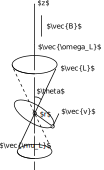
\includegraphics[width=0.15\textwidth]{v4_1}
    \caption{Прецессия электронной орбиты в магнитном поле}
    \figmark{electron orbit}
\end{wrapfigure}

Рассмотрим теперь случай, когда электрон исходно обладает некоторым
орбитальным моментом импульса $L=mvr$ и, соответственно,
магнитным моментом $\mu_L= \frac12 e v r$.
Пусть момент импульса $\vec{L}$ лежит в плоскости
рис.~\figref{electron orbit} и направлен под углом $\theta$ к некоторой оси $z$.
Орбитальное движение электрона эквивалентно витку с током,
магнитный момент которого $\vec{\mu}_L$ пропорционален $\vec{L}$
и направлен против него (поскольку заряд электрона отрицателен).
При включении внешнего магнитного поля с индукцией $B$,
направленной вдоль оси $z$, на электрон начинает
действовать момент силы $\vec{\mu}_L\times \vec{B}$,
перпендикулярный плоскости рис.~\figref{electron orbit} и направленны от
нас. Уравнение движения электрона будет иметь вид
\begin{equation*}
	\frac{d\vec{L}}{dt} = \vec{\mu}_L\times \vec{B}.
\end{equation*}
Как известно из механики, это уравнение описывает движение симметричного волчка
(гироскопа). Его решением является
прецессия электронной орбиты с угловой скоростью
$\omega_{L} = \frac{\mu_L B}{L}$,
направленной вдоль магнитного поля.
Подставляя значения $L$ и $\mu_L$, находим
$\omega_L = \frac{eB}{2m_e}$.
Таким образом, прецессия магнитного момента также происходит с ларморовской частотой
\eqref{Larmor-Omega}
и не зависит от угла $\theta$. Эта прецессия приводит
к дополнительному вращению электрона вокруг поля $B$,
налагающемуся на его орбитальное движение. Нетрудно убедиться, что она
даёт полностью аналогичный \eqref{chi-dia} вклад в диамагнитную восприимчивость.


% Сложно и ненужно // ППВ
%
% Если рассматривать сферически-симметричное распределение заряда
% электрона, то расчёт показывает, что $S = 2/3\pi\average{r^2}$, где
% $\average{r^2}$~--- средний квадрат расстояния электрона от ядра. Поэтому
% \begin{equation*}
% 	\Delta\mu = - \frac{\mu_0 e^2 \average{r^2}}{6m_e}H.
% \end{equation*}
%
% Появление этого момента и приводит к намагничиванию вещества в направлении,
% противоположном полю, т.е. к диамагнетизму. Магнитный момент атома, содержащего
% $Z$ электронов, находится суммированием магнитных моментов отдельных электронов:
% \begin{equation*}
% 	\mu_{\text{ат}} = - \frac{\mu_0 e^2 H}{6m_e}\sum\limits_{i=1}^Z
% \average{r_i^2}.
% \end{equation*}
%
% Сумму можно заменить произведением $Z\average{a^2}$, где $\average{a^2}$~---
% средний квадрат расстояния электронов от ядра. Тогда
% \begin{equation*}
% 	\mu_{\text{ат}} = - \frac{\mu_0 e^2 \average{a^2} Z}{6m_e}H.
% \end{equation*}
% Умножив полученное выражение на число атомов $n$ в единице объёма, получим
% намагниченность $M$:
% \begin{equation*}
% 	M = n\mu_{\text{ат}} = - \frac{\mu_0 e^2 \average{a^2} nZ}{6m_e}H.
% \end{equation*}
% Магнитная восприимчивость
% \begin{equation*}
% 	\chi = \frac{M}{H} = - \frac{\mu_0 e^2 \average{a^2} nZ}{6m_e}.
% \end{equation*}


Из полученного выражения \eqref{chi-dia} для восприимчивости диамагнетиков
следует, что она не зависит ни от температуры, ни от величины напряжённости поля
и растёт пропорционально порядковому номеру элемента.
Диамагнитный эффект свойствен всем веществам (независимо от того, имелся ли у
атома собственный магнитный момент или нет и как он был ориентирован), однако у
некоторых веществ он перекрывается более сильным \important{парамагнитным}
эффектом.


\labsection{Парамагнетизм}

Парамагнетизм характерен для веществ, частицы которых (атомы, ионы, молекулы)
обладают собственным магнитным моментом в отсутствие внешнего магнитного поля.

В парамагнетиках энергия взаимодействия между соседними магнитными моментами
атомов мала по сравнению с тепловой энергией,
поэтому в отсутствие внешнего магнитного поля магнитные моменты
являются полностью разупорядоченными, а намагниченность среды равна нулю.
При помещении во внешнее поле магнитным моментам энергетически выгодно
ориентироваться преимущественно по полю, что и приводит к парамагнитному эффекту.

% Ненужные подробности // ППВ
%
% Этот магнитный момент обусловлен как движением электронов в оболочке атома
% (орбитальный магнитный момент), так и наличием собственных магнитных моментов
% у электронов и ядер (\important{спиновый} магнитный момент).
% Например, в кристаллах медного купороса (CuSO$_4$) содержатся ионы меди,
% у которых электроны на внутренних оболочках имеют суммарный магнитный момент,
% не равный нулю. Изолированный атом меди имеет
% нечётное число электронов (29). На внешней оболочке $4s$ имеется всего один
% электрон, и именно его магнитный момент является магнитным моментом атома меди.
% Поэтому пары меди, как и пары натрия, являются парамагнетиками. Однако при
% переходе в твёрдое состояние (в процессе кристаллизации) атомы меди теряют этот
% электрон, он уходит от своего атома и уже принадлежит всему кристаллу.
% «Застывшие» в узлах решётки ионы меди уже не имеют магнитного момента и поэтому
% не обладают парамагнитным эффектом. Обобществлённые электроны (электроны
% проводимости) образуют электронный газ, который является парамагнетиком,
% поскольку состоит из частиц, обладающих собственным магнитным моментом. Такой
% парамагнетизм называют \important{парамагнетизмом Паули}. Но медь является
% диамагнетиком, и это означает, что диамагнетизм ионов меди преобладает над
% парамагнетизмом свободных электронов.

% Отличительной особенностью парамагнетиков является их слабая намагниченность во
% внешнем магнитном поле при комнатной температуре. В отсутствие магнитного поля
% энергия диполь-дипольного взаимодействия между двумя соседними магнитными
% моментами атомов с межатомным расстоянием $\sim 5 \cdot 10^{-8}$~см составляет
% $\sim 10^{-5}$~эВ, а энергия
% теплового движения на атом $\sim 7,5 \cdot 10^{-2}$~эВ. Такое превосходство
% тепловой энергии приводит к равномерному пространственному распределению
% магнитных моментов, а следовательно, к отсутствию намагниченности у
% парамагнетиков. Но когда начинает действовать внешнее магнитное поле, оно
% выстраивает магнитные моменты так, что магнитных моментов, направленных по полю,
% становится больше, чем направленных против поля, и с ростом поля намагниченность
% парамагнетиков растёт по закону \eqref{magnetization-magnetic vector}.
% Магнитная восприимчивость парамагнетиков всегда положительна, а по величине
% $\chi \sim 10^{-6} \sim 10^{-4}$~(система СИ).

% Упростим вывод до предела!

Оценим температурную зависимость магнитной восприимчивости парамагнетика
в классической модели. Пусть
среднее число атомов в единице объёма равно $n$, а абсолютная величина
магнитного момента атома $\mu_{\text{а}}$.
В магнитном поле с индукцией $B$ энергия магнитного диполя,
составляющего с направлением поля угол $\alpha$, равна
\begin{equation*}
	U = - \mu_{\text{а}}B \cos \alpha
\end{equation*}
и может меняться в диапазоне от $-\mu_{а}B$ до $+\mu_{а}B$
(квантовая механика говорит, что энергия может принимать
ряд дискретных значений в этом же диапазоне).

% \begin{wrapfigure}[]{r}{0.35\textwidth}
% \centering\includegraphics[width=0.2\textwidth]{v4_2}
% 	\caption{Телесный угол $d\Omega$.}
% 	\figmark{dN in dOmega}
% \end{wrapfigure}

Из термодинамики известно, что доля атомов, у которых момент ориентирован
под некоторым углом $\alpha$ к полю, определяется распределением Больцмана:
\begin{equation*}
    dn = \mathrm{const}\cdot  e^{-\tfrac{U(\alpha)}{\kB T}} d\alpha.
\end{equation*}
Пусть внешнее магнитное поле достаточно мало,
так что энергия магнитных моментов атомов в
нём много меньше тепловой: $\mu_{а}B \ll \kB T$.%
\footnote{Для оценки возьмём собственный магнитный момент электрона
$\mu_{e} = e\hbar/2m_e = 9,3 \cdot 10^{-24}\;Дж/Тл$
(магнетон Бора). В магнитном поле с индукцией $B = 1,0$~Тл магнитная энергия
$\mu_{e}~B \sim {10^{-4}}$~эВ --- такая энергия
соответствует температуре $T\sim 1\;К$.
Поэтому в не слишком больших полях и не слишком низких
температурах показатель больцмановской экспоненты действительно много меньше единицы.}
Число атомов, имеющих положительную ($\alpha > 0$) проекцию на направление $\vec{B}$ может
быть записана как
\[
n_{+} = n_0 e^{\mu_{а}B/\kB T}\approx n_0\left(1+\frac{\mu_{а} B}{\kB T}\right),
\]
где мы воспользовались разложением экспоненты от малого параметра,
а $n_0$ --- некоторая нормировочная константа. Для атомов с отрицательной
проекцией момента ($\alpha < 0$):
\[
n_{-} = n_0 e^{-\mu_{а}B/\kB T}\approx n_0\left(1-\frac{\mu_{а} B}{\kB T}\right)
\]
Здесь с учётом нормировки $n_{+} + n_{-} = n$, имеем $n_0 \approx n/2$.

Суммарный магнитный момент единицы объёма можно оценить как
\[
M \sim n_{+}\mu_{а} + n_{-}\cdot (-\mu_{а}) \approx
\frac{\mu_{а}^2 n}{\kB T} B.
\]
Более аккуратное усреднение по углам даст поправочный множитель порядка единицы
(в классической модели получается коэффициент $1/3$).

Таким образом, парамагнитная восприимчивость равна
\begin{equation}
    \eqmark{chi-para}
    \chi_{пар} \sim \frac{\mu_{\text{а}}^2 \mu_0 n}{3\kB T}\propto \frac{1}{T}.
\end{equation}
Температурная зависимость восприимчивости парамагнетиков вида~$\chi\propto 1/T$ называется
\important{законом Кюри}.

% Сложный вывод, при том нестрогий!
%
% Число атомов, магнитные моменты которых направлены под углами
% от $\alpha$ до
% $\alpha + d\alpha$ к полю, определяется распределением Больцмана:
% \begin{equation*}
%     dn = n_0 e^{-\tfrac{U}{\kB T}} \frac{d\Omega}{4\pi},
% \end{equation*}
% где $d\Omega = 2\pi\sin \alpha~d\alpha$ --- телесный угол, соответствующий интервалу
% $(\alpha;\alpha+d\alpha)$ (рис.~\figref{dN in dOmega}),
% $n_0$ -- нормировочная константа.
% Из условия нормировки находим
% \[
% n = n_0 \int\limits_0^\pi e^{\frac{\mu_{\text{а}} B \cos \alpha}{\kB T}}
% \sin \alpha~d\alpha.
% \]
% Полное число атомов в единице объёма
% \begin{equation}
% 	\eqmark{total number of atoms}
% 	N = 2\pi N_0 \int\limits_0^\pi e^{\frac{\mu_{\text{Б}} B \cos \alpha}{\kB T}}
% \sin \alpha~d\alpha.
% \end{equation}
% Проекция магнитного момента атома на направление поля равна
% $\mu_{\text{a}} \cos \alpha $, поэтому суммарный магнитный момент всех атомов единицы
% объема будет равен
% \[
% M = \int\limits_{0}^{\pi} \mu_{а} \cos \alpha dn.
% \]
% Вычисления сильно упрощаются, если энергия атома в магнитном поле мала по сравнению
% с тепловой энергией $\mu_{а} B \ll \kB T$. Тогда, если воспользоваться разложением
% экспоненты $e^{-U/\kB T}\approx 1 + \frac{U}{\kB T}$, нетрудно получить:
% \begin{equation}
% \eqmark{total magnetic moment}
% %
% % n_0 \int\limits_0^\pi \mu_{\text{а}} \cos \alpha \exp
% % \left(\frac{\mu_{\text{а}} B \cos \alpha}{\kB T}\right) \sin \alpha~d\alpha.
% \end{equation}
% В этом приближении из совместного решения \eqref{total number of atoms} и
% \eqref{total magnetic moment} получим, что намагниченность


В сверхсильных полях, когда магнитная энергия внутриатомного диполя сравнима с
тепловой ($B \sim 10^3$~Тл при комнатной температуре), все магнитные моменты в
парамагнетике могут ориентироваться по полю~--- наступает \important{магнитное насыщение}.

В случае парамагнетизма свободных электронов, образующих электронный газ в
металлах, не все электроны могут участвовать в переориентировке своих магнитных
моментов, а только небольшая часть, которая пропорциональна тепловой энергии
$\kB T$ (квантовый эффект). Поэтому у некоторых металлов парамагнетизм не зависит
от температуры.

\labsection{Ферромагнетизм}

Помимо диа- и парамагнетиков, которые слабо реагируют на внешнее магнитное поле,
в природе существуют вещества, способные сильно намагничиваться даже в небольших
магнитных полях. Такие вещества относят к классу ферромагнетиков. Это~---
железо, никель, кобальт, гадолиний и многочисленные сплавы этих металлов между
собой и с другими металлами. Ферромагнитными свойствами обладают некоторые
сплавы элементов, которые порознь не являются ферромагнитными (например, сплавы
меди и марганца), и ряд неметаллических веществ (ферриты). Ферромагнитные явления
сложны и многообразны, и мы ограничимся изложением лишь некоторых основных фактов.

Зависимость намагниченности $M$ от напряжённости магнитного поля $H$ у всех
ферромагнетиков оказывается нелинейной: магнитная восприимчивость
$\chi=\chi(H)$ у ферромагнетиков не является константой и зависит от $H$.
Если у диа- и парамагнетиков $\chi$ составляет всего $10^{-8}$~--~$10^{-4}$, то у
ферромагнетиков магнитная восприимчивость достигает значений $10^3$~--~$10^4$.
Кроме того, у ферромагнетиков (особенно монокристаллических)
магнитная восприимчивость $\chi$ может иметь тензорный характер
(векторы $\vec{M}$ и $\vec{H}$ не сонаправлены),
обусловленный анизотропией кристаллической решетки.

% Этому место в начале раздела // ППВ
%
% Степень намагничивания ферромагнитного вещества можно
% характеризовать не только вектором намагниченности $M$, но и вектором магнитной
% индукции $B$ в данном веществе:
% \begin{equation*}
% 	B =\mu_0 (H + M).
% \end{equation*}
% При $M = \chi H$
% \begin{equation}
% 	B = \mu_0 (1 + \chi)H = \mu \mu_0 H.
% \end{equation}
% \todo [author=Tiffani]{В формуле 4.4 была ошибка. Исправила.}
%
% Величина $\mu = 1+ \chi$ носит название магнитной проницаемости вещества. Если у
% диа- и парамагнетиков $\mu$ отличается от единицы всего на сотые доли процента,
% то у ферромагнетиков $\mu$ практически совпадает с $\chi$ (в системе СИ).
%
% Отметим, что в системе СГС, где $B = (1 + 4\pi \chi) H$, $\chi$ в $4\pi$ раз
% меньше, чем в системе СИ.

Как и в случае парамагнетиков, атомы ферромагнетика обладают собственным магнитным
моментом. Однако даже в отсутствие внешнего магнитного поля атомы ферромагнетика
способны образовывать упорядоченные структуры (\important{домены}),
в которых все магнитные моменты ориентированы практически в одном направлении.
Таким образом, каждый отдельный атом испытывает влияние не только внешнего
поля, но и поля, созданного ``дружным коллективом'' его соседей.
В качестве простейшей эмпирической модели, описывающей такую ситуацию, можно
рассмотреть
так называемую модель \important{среднего поля}: предположим, что намагниченность
элемента среды пропорциональна некоторому эффективному полю $H_{эфф}$
складывающемуся из поля $\vec{H}$ в данной точке, созданного сторонними токами, и среднего ``коллективного'' поля,
пропорционального величине намагниченности $\vec{M}$:
\begin{equation}
\eqmark{average-field}
\vec{M} = \chi_{пар} \vec{H}_{эфф},\qquad \vec{H}_{эфф} = \vec{H} + \beta \vec{M},
\end{equation}
где $\chi_{пар}$ --- парамагнитная восприимчивость отдельного атома
\eqref{chi-para}, $\beta$~--- некоторая безразмерная константа, определяемая из опыта.

Модель среднего поля позволяет уточнить закон Кюри.
Определяя магнитную восприимчивость по-прежнему как $\chi = M/H$, найдём
из \eqref{average-field}:
\begin{equation}
    \eqmark{Kuri-Weiss}
    \chi = \frac{1}{\frac{1}{\chi_{пар}}-\beta} \propto
    \frac{1}{T-\Theta},
\end{equation}
где параметр $\Theta = \beta \frac{\mu_{a}^2\mu_0 n}{3\kB}$ имеет размерность
температуры.

Соотношение \eqref{Kuri-Weiss} называют
\important{законом Кюри--Вейсса}. В частности, этот закон предсказывает
существование особой точки, в которой $\chi$ обращается в бесконечность.
Действительно, существует температура $\Theta_К$, называемая
\important{точкой Кюри}, в которой имеет место фазовый переход (2-го рода) между
парамагнитным (при $T>\Theta_К$) и ферромагнитным состоянием среды
при $T < \Theta_К$. Закон Кюри--Вейсса удовлетворительно выполняется
вдали от $\Theta_К$, однако нарушается при приближении к точке перехода
$T \to \Theta_К$, где модель среднего поля становится слишком груба.
Поэтому параметр $\Theta$ в \eqref{Kuri-Weiss} несколько
отличается от температуры Кюри: как правило, $\Theta_К < \Theta$.

Остановимся кратко на причине, по которой соседним магнитным моментам выгодно
объединяться в домены. В первую очередь подчеркнём, что
магнитное (диполь-дипольное) взаимодействие между атомами
не может привести к упорядочению системы.
Чтобы в этом убедиться, достаточно оценить энергию такого взаимодействия:
из квантовой механики известно, что магнитный момент атома
по порядку величины равен~$\mu_Б = 9,3\cdot 10^{-24}\; Дж/Тл$
(\emph{магнетон Бора}),
характерное расстояние между атомами~$a\sim 2 \cdot 10^{-10}\;м$,
тогда характерное межатомное магнитное поле
$B \sim \mu_0 \frac{\mu_Б}{a^3} \sim 1\;Тл$, и характерная энергия
энергия диполь-дипольного взаимодействия
$U_{дип.}\sim \mu_Б B \sim 10^{-4}\;эВ$.
При такой энергии связи тепловое движение обеспечит полное
разупорядочение уже при $T\sim 1\;К$.

Единственное взаимодействие, которое способно выстроить в ряд магнитные
моменты электронов в атомах при температурах порядка комнатной, --- это
\emph{электростатическое} взаимодействие
(его энергия на несколько порядков больше магнитной:
$e^2/(4\pi\varepsilon_0 a) \sim 1\;эВ$).
Как следует из квантовой механики, если магнитные моменты (или спины) электронов
соседних атомов сонаправлены,
их электростатическое отталкивание становится \emph{меньше}.
Таким образом, магнитным моментам атомов энергетически выгодно ориентироваться
в одном направлении. Такое явление получило название
\important{обменного взаимодействия}.

% Написано крайне не аккуратно // ППВ
%
% Учёт взаимодействия
% элементарных магнитных моментов, заключающийся в прибавлении к макроскопическому
% полю $H$ поля, пропорционального намагниченности (подобно приёму учёта поля
% соседей в диэлектрике введением поля поляризуемости с коэффициентом $4\pi/3$),
% противоречит опыту, поэтому вводится эмпирическая постоянная $\lambda$, т.е.
% вместо поля $H$ нужно использовать величину $H + \lambda M$.  Используя
% полученную формулу для намагниченности, получим
% \begin{equation*}
% 	M = \frac{\mu_{\text{Б}}^2 \mu_0 N}{3\kB T}(H + \lambda M)
% \end{equation*}
% и соответственно
% \begin{equation*}
% 	\chi = \frac{\mu_{\text{Б}}^2 \mu_0 N}{3k(T - \Theta)},
% \end{equation*}
% где $\Theta = \mu_{\text{Б}}^2 \mu_0 N / 3k$ имеет размерность температуры.

% Зависимость  $1/\chi$  от температуры называется законом Кюри-Вейса и
% представляется прямой, пересечение которой с осью абсцисс определяет
% характеристическую температуру. Если эта величина положительна, существует
% температура, ниже которой восприимчивость принимает огромные значения. Это
% справедливо для ферромагнетиков, остальные вещества ведут себя подобным образом
% вблизи абсолютного нуля. Для $T>\Theta$ ферромагнетики ведут себя как
% парамагнетики.

% Результаты экспериментов для постоянной $\lambda$ для ферромагнетиков дают
% величину $10^4$, т.е.поле, пропорциональное намагниченности, оказывается порядка
% $10^7$~эрстед (хотя поле соседних узлов решетки около $10^3$~эрстед).

% Огромная величина поля, связанная с намагниченностью, нашла своё объяснение в
% квантовой теории при введении так называемого обменного взаимодействия
% электронов, т.е. эти силы имеют электростатическую природу. Характерная энергия
% этого взаимодействия порядка $10^{-13}$~эрг. В результате этого взаимодействия
% устойчивое состояние ферромагнетика соответствует полной намагниченности, хотя в
% реальности   оказываются намагничены микроскопические области размером порядка
% несколько микрометров, а в целом образец ненамагничен. Следует  отметить, что
% величина магнитного поля в домене примерно совпадает с полем насыщения
% ферромагнетика. Области полной намагниченности назвали доменами, размер которых
% является следствием конкурирующих вкладов в полную энергию ферромагнетика:
% обменной энергии, энергии анизотропии и магнитной энергии. Пример разбиения
% кристалла на домены приведён на рисунке (??4.3.1??), где полная энергия
% уменьшается от a) до в).
% \todo [author=Tiffani]{Присутствует ссылка на рис. 4.3.1, которого нет в папке.
% См. примечание ниже.}
%
% \todo [author=Tiffani]{Здесь должна быть картинка 4.3.1, но она не соответствует
% той, что в ворде. Нужную картинку в папке с картинками не нашла.}

\begin{wrapfigure}[]{r}{0.4\textwidth}
    \centering\includegraphics[width=0.35\textwidth]{Chapter_4/domains}
    \caption{Доменная структура ферромагнетика при слабом (слева)
    и сильном (справа) внешнем поле}
    \figmark{domains}
\end{wrapfigure}

С другой стороны, магнитное диполь-дипольное взаимодействие между доменами препятствуют
выстраиванию всех магнитных моментов среды в одном направлении.
Действительно, энергия такого взаимодействия будет минимальной
при \emph{анти}параллельном расположении магнитных моментов соседних элементов среды.
Поэтому при определённом поперечном размере домена оказывается
энергетически выгодно иметь соседний домен с противоположно ориентированным моментом
(см. рис.~\figref{domains}, слева).
Наложение внешнего поля заставляет домены ориентироваться
по нему, что приводит к резкому увеличению намагниченности образца, а при
достаточно большом поле достигается состояние \important{насыщения},
когда все домены ориентируются по полю (см. рис.~\figref{domains}, справа).

% Между доменами существуют переходные слои (в железе их толщина $\sim
% 10^{-5}$~см), в которых направление магнитного момента атомов плавно переходит
% от направления в одном домене к направлению в соседнем. Такие слои называют
% «стенками Блоха». Энергия этих слоёв пропорциональна их площади.
% \todo [author=Tiffani]{Неплохо было бы выделять термины вроде «стенками Блоха» и
% «скачки Баркгаузена» курсивом или жирным шрифтом при первом упоминании в
% тексте.}

\labsection{Ферромагнитный гистерезис}

Если состояние некоторой системы зависит не только от мгновенных значений
внешних параметров, но от истории их изменений, говорят, что
в системы имеет место \important(гистерезис).

Именно такими свойствами обладает магнитный момент ферромагнитного образца
как функция напряжённости поля $M(H)$. В частности,
система может оказаться намагниченной, даже когда внешнее поле выключено ---
этим объясняется существование постоянных магнитов. Рассмотрим данное явление подробнее.

Пусть ферромагнетик находится исходно в ненамагниченном состоянии
($M = 0$). Медленно увеличивая поле $H$ в образце, получим зависимость
$M(H)$, которую называют \emph{начальной кривой намагничивания}. Эту кривую обычно
разделяют на пять условных участков (рис.~\figref{magnetization curve}).

Участок 1~--- область обратимого намагничивания, где $M =\chi H$. В этой области
происходят процессы упругого смещения границ доменов: увеличивается размер тех
доменов, магнитный момент которых близок к направлению магнитного поля, и
уменьшаются размеры доменов с противоположным направлением магнитного момента.

\begin{wrapfigure}[]{r}{0.5\textwidth}
    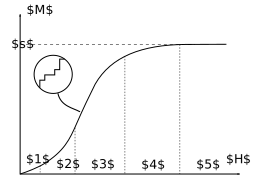
\includegraphics[width=0.4\textwidth]{v4_3}
    \caption{Начальная кривая намагничивания ферромагнетика}
    \figmark{magnetization curve}
\end{wrapfigure}

Участок 2 характеризуется квадратичной зависимостью $M$ от $H$. В этой области
также идёт процесс обратимого смещения границ, но проявляется нелинейный характер
зависимости намагниченности от поля.

Область максимальной скорости роста намагниченности 3 соответствует необратимым
смещениям стенок между доменами (<<стенок Блоха>>):
им приходится преодолевать <<препятствия>> в виде примесей,
дислокаций и дефектов кристаллической решётки.
Когда стенка наталкивается на такое препятствие, она останавливается и держится,
пока поле не достигнет порогового значения, при котором она внезапно
срывается. Таким образом, движение доменной стенки приобретает скачкообразный
характер (<<скачки Баркгаузена>>).

% Фрагмент кривой намагничивания в этой области в увеличенном масштабе показан на
% рис.~\figref{magnetization curve}. Скачкообразное движение стенок приводит к
% быстрому изменению намагниченности образца, что вызывает появление вихревых
% токов, а следовательно, диссипацию энергии. Выделение тепла внутри образца и
% приводит к необратимому движению доменных стенок.

В достаточно сильных полях движение стенок прекращается и энергетически
выгодным становится поворот магнитных моментов тех оставшихся доменов, у которых
магнитный момент не совпадает с направлением поля (область 4).

И, наконец, при некотором значении поля (участок 5) все магнитные моменты
выстраиваются по полю~--- намагниченность образца достигает \emph{насыщения}.

% Повторы! // ППВ
%
% \begin{wrapfigure}[12]{r}{0.35\textwidth}
% 	\includegraphics[width=0.2\textwidth]{v4_4}
% 	\caption{Зависимость намагниченности насыщения ферромагнетика от
% температуры}
% 	\figmark{magnetization-temperature}
% \end{wrapfigure}
%
% Магнитные и другие физические свойства ферромагнетиков существенным образом
% зависят от температуры. Например, намагниченность насыщения $M_s$ имеет
% наибольшее значение при $T = 0~(M_s (0))$ и монотонно уменьшается до нуля при
% температуре $\Theta$, которую называют ферромагнитной точкой Кюри
% (рис.~\figref{magnetization-temperature}).
%
% \todo [author=Tiffani]{Обозначения на рис. 4.4 не имеют ничего общего с
% действительностью.}
%
% Выше  этой температуры $\Theta$ тепловое движение разупорядочивает магнитную
% структуру доменов и ферромагнетик переходит в парамагнитное состояние. В
% отсутствие внешнего магнитного поля переход ферромагнетик~---парамагнетик
% является фазовым переходом II рода.
%
% Мы уже знаем, что для парамагнетиков зависимость магнитной восприимчивости от
% температуры имеет вид закона Кюри ($\chi \sim 1/T$). Аналогичная зависимость
% восприимчивости ферромагнетиков от температуры при температурах выше $\Theta$
% описывается законом Кюри-Вейсса:
% \begin{equation*}
% 	\chi = \frac{C}{T - \Theta_p},
% \end{equation*}
% где $C$ -- постоянная Кюри, $\Theta_p$ -- температура Кюри (как правило
% $\Theta_p > 0$).

На практике магнитные свойства ферромагнетиков обычно изучают путём измерения
зависимости индукции магнитного поля $B(H)$ от напряжённости магнитного поля $H$ в
веществе. Исследование образца, естественно, начинают с полностью
размагниченного состояния ($H = 0$, $B = 0$). Если теперь монотонно увеличивать
напряжённость поля $H$, то изменение $B$ происходит по рассмотренной выше
начальной кривой намагничивания с учётом соотношения \eqref{fieldB}
(кривая $OA$ на рис.~\figref{hysteresis curve}).

Наклон кривой намагничивания принято характеризовать
\important{дифференциальной} магнитной проницаемостью
\begin{equation}
    \eqmark{mu-diff}
    \mu_{\text{дифф}} \equiv \frac{1}{\mu_0} \frac{dB}{dH}.
\end{equation}
С ростом $H$ величина $\mu_{дифф}$ сначала растёт (участки 1 и 2),
затем с середины участка 3 начинает резко падать,
приближаясь к единице при насыщении.

\begin{wrapfigure}{r}{0.4\textwidth}
    \pic{0.38\textwidth}{v4_8}
    \caption{Начальная кривая намагниченности и кривая гистерезиса}
    \figmark{hysteresis curve}
\end{wrapfigure}

Доведём систему до некоторой точки $A$, лежащей в области
насыщения (здесь $B_s$~--- \important{индукция насыщения}\footnote[1]{s~--- saturated
(англ.)~--- насыщенный}), и начнём уменьшать напряжённость поля $H$.
Поскольку между доменами есть трение, обратный путь
пойдёт не по начальной кривой, а выше неё.

При выключения внешних полей, то есть при достижении $H = 0$,
в образце сохраняется некоторое собственное намагничивание.
Соответствующее значение индукции $B_r$
называют \important{остаточной индукцей}\footnote[2]{r~--- remained (англ.)~--- оставшийся}.

Значение $B = 0$ достигается лишь при некотором отрицательном значении
$H = - H_c$. Величина $H_c$ называется
\important{коэрцитивным полем}\footnote[3]{c~--- coercive (англ.)~--- принудительный}.
Среди ферромагнетиков принято различать \emph{магнитожёсткие}
(с $H_c > 10^3$~А/м) и \emph{магнитомягкие матералы}. В точке $C$
наступает насыщение для намагничивания в противоположную сторону.

Если теперь попробовать вернуться в точку $A$, вновь наращивая поле,
получим некоторый замкнутый цикл (\important{кривую гистерезиса}). Если
в точке $A$ насыщение не достигается, то аналогичным образом можно получить
цикл меньшей площади (заметим, что поскольку процессы, происходящие
в системе, необратимы, цикл будет вообще говоря незамкнутым).

Отметим, что \emph{площадь петли} гистерезиса ферромагнетика на плоскости
$H$--$B$ есть энергия, необратимо выделяющейся в виде тепла в единице
объёма вещества за один цикл:
\begin{equation}
    \eqmark{HdB}
    \Delta w = -\oint {HdB}
\end{equation}
(см. далее вывод формулы \eqref{magnetic-energy}).

% Можно короче. // ППВ
%
% Магнитное состояние вещества
% характеризуется теперь точками кривой $CA$, лежащими низке начальной кривой
% намагничивания. Строго говоря, кривая не пройдёт и через точку $A$, а окажется
% ниже неё. Вновь уменьшая магнитное поле, мы пройдём поэтому по кривой,
% расположенной ниже кривой $AC$, не попадём в точку $C$ и начнём движение к $A$
% по некоторому новому пути. Магнитные циклы, таким образом, обычно оказываются
% незамкнутыми. Многократно проходя один и тот же цикл, образец приближается к
% предельному замкнутому циклу (кривой гистерезиса), не зависящему от начального
% состояния. Описанная картина наиболее отчётливо проявляется в тех случаях, когда
% образец не доводится до насыщения. При заходе в область насыщения намагничивание
% зависит главным образом от $H$ и лишь в очень слабой степени от истории образца.
% Предельные циклы устанавливаются при этом сразу (т. е. при однократном
% прохождении цикла) или почти сразу. В соответствии с этим на
% рис.~\figref{magnetization curve} не сделано различия между частным циклом и
% предельным.


\labsection{Измерение напряжённости и индукции магнитного поля}

\paragraph{Размагничивающий фактор.}
Когда говорят о кривой намагничивания $B(H)$,
речь идёт о \emph{локальной} связи между
индукцией и напряжённостью магнитного поля в каждой точке среды.
При этом под $H$ имеется в виду не внешнее магнитное поле,
а именно поле \emph{внутри} данного материала. Поскольку непосредственному
измерению легче всего поддаётся именно внешнее поле $\vec{H}_{0}$,
создаваемое сторонними токами без образца, необходимо установить связь
между $\vec{H}$ и $\vec{H}_0$ (заметим, что $\vec{B}_0=\vec{H}_0$).

Из условия непрерывности касательной компоненты вектора $\vec{H}$ следует,
что $\vec{H}$ совпадает $\vec{H}_{0}$ только если во всех точках образца
$\vec{H} \parallel \vec{H}_{0}$.
Такое возможно, например, в пределе \emph{бесконечно длинного соленоида} либо
для \emph{тонкого тора}.
В общем случае $\vec{H}_0 \ne \vec{H}$.

Рассмотрим магнетик, помещённый в однородное внешнее поле $\vec{H}_0$.
Разность между внешним полем и полем в образце принято называть
\important{размагничивающим полем}:
$\vec{H}_{разм} = \vec{H}_0 - \vec{H}$.
Если форма образца такова, что его намагниченность можно считать
практически постоянной $\vec{M}\approx\mathrm{const}$ (за исключением,
возможно, незначительных ``краевых эффектов''), можно ввести
коэффициент пропорциональности между $\vec{H}_{разм}$ и намагниченностью $\vec{M}$,
называемый \important{размагничивающим фактором}:
\[
N_{разм} = \frac{H_0-H}{M}.
\]
Для однородного образца размагничивающий фактор зависит
только от его формы и ориентации в поле.
С учётом \eqref{fieldB} нетрудно убедиться, что его величина может меняться в пределах $0\le N_{разм} \le 1$.

Для образца с известным $N_{разм}$, изготовленного из материала
c проницаемостью $\chi$, помещённого во внешнее поле $H_0$, имеем
$H_0 - H = N M$, $M=\chi H$, откуда
\[
M = \frac{\chi H_0}{1+N_{разм}\chi}.
\]

Аналитические выражения для $N_{разм}$ могут быть получены только для тел
простейшей формы. В частности
\begin{itemize}
    \item бесконечно длинный цилиндр: продольное поле~--- $N_{разм} = 0$,
          поперечное поле~--- $N_{разм} = 1/2$;
    \item шар $N_{разм} = 1/3$;
    \item бесконечно тонкая пластинка в поперечном поле $N_{разм} = 1$,
          в продольном --- $N_{разм} = 0$.
\end{itemize}

Заметим, что для диа- и парамагнетиков $|\chi|\ll 1$, поэтому отличием $H$ от
$H_0$ для них можно, как правило, пренебречь.

% Сложно и ненужно // ППВ
%
% На практике
% для снятия петли гистерезиса мы обычно помещаем во внешнее однородное магнитное
% поле ферромагнитный образец, имеющий конечные размеры. Однородная
% намагниченность по всему объёму образца будет иметь место только для образцов,
% имеющих форму эллипсоидов вращения, в частности, для шара, для очень тонкой
% пластинки и для тонкого и длинного цилиндра. Во всех этих случаях величина
% магнитного поля внутри образца будет меньше внешнего магнитного поля. Рассмотрим
% в качестве примера образец, имеющий форму цилиндра длиной $l$ и диаметром $d (d
% \ll l)$.
%
% Пусть ось симметрии цилиндра направлена вдоль внешнего магнитного поля величиной
% $H_0$. Цилиндр будет практически однородно намагничен с некоторой
% намагниченностью $M$. Найдём величину индукции магнитного поля на оси цилиндра в
% точке, равноудалённой от торцов. С одной стороны, используя связь между $B$, $M$
% и $H$, можно записать
% \begin{equation}
% 	\eqmark{cylinder-B(H)}
% 	B_{\text{вн}} = \mu_0 (H_{\text{вн}} + M),
% \end{equation}
% где $H_{\text{вн}}$~--- величина поля внутри образца. С другой стороны,
% намагниченный цилиндр можно рассматривать как цилиндрическую поверхность
% диаметра $d$ с однородным кольцевым поверхностным током плотностью:
% \begin{equation*}
% 	j = M.
% \end{equation*}
% Эти молекулярные токи создают собственное магнитное поле, которое по направлению
% совпадает с внешним полем $H_0$, а по величине равно\footnote[4]{См. [4]. Задача
% № 5.5.}:
%
% \todo [author=Tiffani]{Возможно, лучше вместо ``См. [4]. Задача № 5.5.''
% написать ``См. в приложении'', т.к. задача будет в приложении к этой главе}
% \begin{equation*}
% 	H_{\text{мол}} = \frac{Ml}{\sqrt{l^2 + d^2}}.
% \end{equation*}
%
% Индукцию магнитного поля найдём как суперпозицию внешнего поля и поля
% молекулярных токов:
% \begin{equation}
% 	\eqmark{B(H)-molecular current}
% 	B_{\text{вн}} = \mu_0\left( H_0 + \frac{Ml}{\sqrt{l^2 + d^2}} \right).
% \end{equation}
% Приравнивая \eqref{cylinder-B(H)} и \eqref{B(H)-molecular current}, получим
% \begin{equation*}
% 	H_0 + \frac{Ml}{\sqrt{l^2 + d^2}} = H_{\text{вн}} + M.
% \end{equation*}
%
% Разность между внешним и внутренним полями называют размагничивающим полем:
% \begin{equation*}
% 	H_{\text{разм}} = H_0 - H_{\text{вн}} = \left( 1 - \frac{1}{\sqrt{1 + \left(
% \frac{d}{l} \right)^2}} \right) M = N_p M.
% \end{equation*}
% И тогда связь поля внутри и поля внешнего
% \begin{equation*}
% 	H_{\text{вн}} = \frac{H_0}{1 + N_p M},
% \end{equation*}
% а  магнитная проницаемость образца
% \begin{equation*}
% 	\chi_{\text{обр}} = \frac{\chi}{1 + N_p \chi}.
% \end{equation*}
% \important{Коэффициент пропорциональности между размагничивающим полем и
% намагниченностью образца обозначают через $N_p$ и называют размагничивающим
% фактором или коэффициентом размагничивания. Его величина зависит только от
% геометрических размеров образца и может изменяться в пределах от 0 до 1.}

% Полученное выражение для $N_p$ цилиндра с параметрами $d/l \ll 1$ всё равно
% остаётся приближённым выражением, хотя и с достаточно хорошим приближением. А
% вот точные значения размагничивающего фактора могут быть рассчитаны только в
% отдельных частных случаях:

\paragraph{Измерения в тороидальном образце.}

\begin{wrapfigure}[13]{r}{0.4\textwidth}
    \pic{0.38\textwidth}{v4_5}
    \caption{Тороидальный образец с намагничивающей обмоткой}
    \figmark{toroid}
\end{wrapfigure}

В лабораторных условиях для исследования зависимости $B(H)$ ферромагнитных
материалов обычно используют образцы тороидальной формы. Если на тор намотать
равномерную намагничивающую обмотку (рис.~\figref{toroid}), то поле $H$ внутри
тора на окружности радиуса $R$ будет пропорционально току $I$ в обмотке, а его
величину можно рассчитать по теореме о циркуляции вектора $H$:
\begin{equation}
    \eqmark{H-toroid}
    H = \frac{IN_0}{2\pi R},
\end{equation}
где $N_0$~--- число витков намагничивающей обмотки. Напряжённость магнитного
поля в тороидальном образце зависит от $R$, поэтому
намагниченность образца можно считать однородной при $r \ll R$, где $r$ ---
радиус сечения тора.

\begin{wrapfigure}{r}{0.4\textwidth}
    \pic{0.38\textwidth}{v4_6}
    \caption{Тороидальная катушка с разрезом}
    \figmark{toroidal coil-cut}
\end{wrapfigure}

\paragraph{Поле в зазоре электромагнита.}
Рассмотрим теперь тороидальную катушку, в которой сделан узкий разрез толщиной
$\delta$ ($\delta \ll r \ll R$) (рис.~\figref{toroidal coil-cut}).

Пусть $H_1$~--- напряжённость магнитного поля в
образце, а $H_2$~--- в зазоре. По теореме о циркуляции вектора $H$ имеем
\begin{equation}
	\eqmark{H-toroid-cut}
	\oint {Hdl} = H_1 (2\pi R - \delta) + H_2 \delta  = N_0 I.
\end{equation}

Воспользуемся нeпрерывностью нормальных составляющих вектора магнитной
индукции $B$ на границах разреза. В образце имеем $B_1 = \mu_0 \mu H_1$,
а в зазоре $B_2 = \mu_0 H_2$, поэтому приравнивая $B_1$ и $B_2$, найдём:
\[H_2 = \mu H_1.\]
Подставляя это в \eqref{H-toroid-cut}, получим
\begin{equation}
	\eqmark{H1-toroid-inside}
	H_1 = \frac{N_0 I}{2\pi R + (\mu - 1)\delta},\quad H_2 = \mu H_1
\end{equation}
Отметим, прежде всего, что напряжённости поля в образце и в зазоре
(при $\mu = \mathrm{const}$) пропорциональны силе намагничивающего тока.
После того, как установлена величина коэффициента
пропорциональности, измерение напряжённости может быть заменено измерением тока.

При наличии даже небольшого зазора второе слагаемое в знаменателе
\eqref{H1-toroid-inside} может существенно превосходить первое из-за большой величины
$\mu\gg1$. Тогда полагая $\mu\gg \frac{2\pi R}{\delta}\gg 1$, из
\eqref{H-toroid-cut} найдём поле в зазоре:
\begin{equation}
	\eqmark{H2-toroid-big gap}
	H_2 \approx \frac{N_0 I}{\delta}.
\end{equation}
Интересно, что из \eqref{H2-toroid-big gap} следует, что поле в зазоре
электромагнита практически не зависит ни от размеров и формы магнитного ярма (части
магнитной цепи, заполненной веществом с большим $\mu$), ни от его материала.

% Воздушные зазоры электромагнитов можно использовать для исследования
% ферромагнитных образцов. А можно и не использовать.


\paragraph{Измерение индукции в образце.}
Одни из простейших и в то же время надёжных методов измерения
индукции $B$ внутри некоторого образца основан
на законе электромагнитной индукции.
Электродвижущая сила, возникающая в контуре при изменении
пронизывающего контур магнитного потока $\Phi(B)$, равна
\begin{equation}
	\eqmark{EMF-magnetic flux}
	\mathcal{E} = - \frac{d\Phi (B)}{dt},
\end{equation}
Так как магнитный поток $\Phi (B)=BS$ равен произведению индукции $B$ на площадь
образца $S$, формула \eqref{EMF-magnetic flux} позволяет определить производную от
индукции $B$. Чтобы измерить саму величину $B=-\frac1{S}\int \mathcal{E} dt$,
необходимо иметь некоторое интегрирующее устройство.
В качестве такового может быть применён милливеберметр (работа 3.4.1),
баллистический гальванометр (работа 3.4.4), интегрирующая $RC$-цепочка
(работа 3.4.5). В современной практике всё чаще применяется цифровое интегрирование.

Следует обратить внимание, что при измерениях в переменном поле
в образцах с большим $\mu$ и хорошей электропроводностью
нельзя не учитывать конечную глубину
проникновения поля в образец (\emph{скин-эффект}), равную%
\footnote{См. \textit{Сивухин Д.В.} Общий курс физики, Т.~3, \S 144.}
\[
\delta \sim \sqrt{\frac{\rho}{\mu \mu_0 f}},
\]
где $\rho$ --- удельное сопротивление, $f$ --- частота колебаний поля.
Например, при $f=50\;Гц$ для чистого железа ($\rho \approx 10^{-7}\;Ом\cdot м$,
$\mu \sim 10^3$) имеем $\delta \sim 1\;мм$.


\labsection{Энергия и силы в магнитном поле}

\paragraph{Энергия поля.}
Рассмотрим соленоид длиной $l$, площадью $S$ и числом витков $N$,
заполненный магнетиком с известным законом зависимости индукции от напряжённости
поля $B(H)$ (или $H(B)$). Подключим соленоид к источнику $\mathcal{E}$.
Пусть омическое сопротивление цепи равно $R$.
Плавно (квазистатически) увеличим ток в цепи до некоторого значения
$I$, так что напряжённость в соленоиде станет равна
$H = \frac{N}{l} I$. Закон Ома в цепи соленоида имеет вид
\begin{equation}
    \eqmark{OhmLaw-solenoid}
\mathcal{E} - IR = \frac{d\Phi}{dt},
\end{equation}
где правая часть отвечает ЭДС индукции, $\Phi = NBS$ --- магнитный поток в
цепи.

Магнитная энергия $W_М$, запасённая в соленоиде, равна работе
источника $A_{ист}=\int \mathcal{E}I\, dt$ за вычетом тепловыделения $Q=\int I^2 R\, dt$.
С~учётом \eqref{OhmLaw-solenoid}, получим
\begin{equation}
    \eqmark{magnetic-energy-full}
W_М = \int\limits_0^t I(\mathcal{E} - I R) dt =
\int\limits_0^t I\frac{d\Phi}{dt} dt = \int I\,d\Phi.
\end{equation}
В последнем равенстве мы перешли от интегрирования
по времени к интегрированию по значениям $\Phi$. Если связь между потоком и током
\emph{линейна}: $\Phi = L I$, где $L=\mathrm{const}$ --- индуктивность, то
справедлива обычная формула для магнитной энергии
\begin{equation}
    \eqmark{magnetic-energy-full-simple}
    W_М = \frac{LI^2}{2} = \frac{\Phi I}{2} = \frac{\Phi^2}{2 L}.
\end{equation}


В случае произвольной геометрии магнетик
можно разбить на элементарные ячейки и определить
\important{объёмную плотности энергии} магнетика: разделив
\eqref{magnetic-energy-full} на объём $V=Sl$ и воспользовавшись соотношениями
$\Phi = NBS$ и $I=lH/N$, получим
\begin{equation}
    \eqmark{magnetic-energy}
 w_М = \int H\,dB.
\end{equation}
В частном случае простых диа- и парамагнетиков, для которых связь
$B=\mu \mu_0 H$ линейна, имеем упрощённую формулу
\begin{equation}
    \eqmark{magnetic-energy-simple}
    w_М = \frac{\mu\mu_0 H^2}{2} = \frac{HB}{2} = \frac{B^2}{2\mu\mu_0}
\end{equation}

Найдём изменение энергии \eqref{magnetic-energy} системы при переходе
по некоторому замкнутому контуру:
\[\Delta w_М = \oint H\,dB.\]
Если все процессы в магнетике обратимы, а функция $H(B)$ будет
определена однозначно, а энергия будет сохраняться: $\Delta w_М =0$.
В ферромагнетиках имеет место гистерезис и функция $B(H)$ однозначной не является.
В таком случае в магнетике имеют место необратимые процессы, а величина
$\Delta w_М = \oint H\,dB <0$ (площадь петли) будет равна потерям энергии на тепловыделение
в образце за один период.

\paragraph{Силы в магнитном поле.}
Задача о силах, действующих на магнетики в магнитном поле, наиболее просто
решается энергетическим методом \emph{виртуальных перемещений}.

Рассмотрим некоторую систему, находящуюся в равновесии,
для которой известна зависимость её магнитной энергии $W_М(x)$
от некоторой (обобщённой) координаты $x$. Пусть под действием
некоторой внешней силы $F$ (положительное направление по оси $x$)
система сместилась от равновесия на малую величину $\delta x$.
При этом сила совершила работу $\delta A = F\delta x$.
Эта работа может пойти на приращение магнитной энергии $\delta W_М$,
а также рассеяться в виде тепла $\delta Q$. Кроме того,
дополнительную работу может совершить источник $\delta A_{ист}$.
Таким образом, закон сохранения энергии имеет вид
\[
F\delta x = \delta W_М - \delta A_{ист} + \delta Q.
\]

Предположим сперва, что магнитный поток в цепи поддерживается постоянным
($\Phi = \mathrm{const}$). Тогда из закона Ома \eqref{OhmLaw-solenoid}
в любой момент имеем $\mathcal{E} = IR$. Домножая на $I$, получим
$\mathcal{E} I = I^2R$,
то есть работа источника $\delta A_{ист}=\mathcal{E}Idt$
идёт целиком на тепловыделение $\delta Q=I^2Rdt$.
Значит, вся работа внешней силы пойдёт на приращение магнитной энергии:
$F \delta x = \delta W_М$. В таком случае внешняя сила равна производной
энергии системы по координате при  $\Phi=\mathrm{const}$ (или $B=\mathrm{const}$):
\begin{equation}
    \eqmark{force-Phi}
    F^{(внеш)}_x = \left(\frac{\partial W_М}{\partial x}\right)_{\Phi}.
\end{equation}

Пусть теперь поддерживается постоянным ток в цепи
($I = \mathrm{const}$). Здесь ситуация оказывается несколько сложнее.
Опять пользуясь законом Ома \eqref{OhmLaw-solenoid}, запишем:
\[
\delta A_{ист}-\delta Q=(\mathcal{E} I - I^2R) dt = I \delta \Phi
% =\delta Q + \delta W_М.
\]
Видно, что вклад источника не учитывать нельзя. Вычисления существенно
упрощаются, если мы имеем дело с материалами, для которых
реализуется \emph{линейная} связь между $\Phi$ и $I$ (и между $H$ и $B$).
В таком случае из \eqref{magnetic-energy-full-simple} имеем
\[
\delta W_М|_{I=\const} = \delta\left(\frac{\Phi I}{2}\right) = \frac12 I \delta \Phi.
\]
Видно, что вклад работы источника по модулю вдвое превосходит изменение
магнитной энергии и противоположен по знаку. Таким образом получаем
$F\delta x = \frac12 I\delta \Phi - I\delta \Phi = - \delta W_М$,
и внешняя сила равна производной
энергии системы по координате при  $I=\mathrm{const}$ (или $H=\mathrm{const}$),
\emph{взятой с обратным знаком}:
\begin{equation}
    F^{(внеш)}_x = -\left(\frac{\partial W_М}{\partial x}\right)_{I}.
\end{equation}
Заметим, что полученная выше формула \eqref{force-Phi} более общая и
справедлива в том числе для ферромагнетиков с нелинейным законом
$H(B)$.


\cleardoublepage
\chapter{Плазма. Газовый разряд}

% \section{Введение}

Как известно, вещество может находиться в трёх агрегатных состояниях~--- твёрдом,
жидком и газообразном, причём эти
состояния последовательно сменяются по мере возрастания температуры. Если~и
дальше нагревать газ, то сначала молекулы диссоциируют на атомы, а~затем и атомы
распадаются на электроны и ионы, так что газ становится \emph{ионизованным},
представляя собой смесь из свободных электронов и ионов, а~также нейтральных
частиц. Если \important{степень ионизации} газа
(отношение числа ионизованных атомов к их полному числу) оказывается достаточно велика, то
такой газ может обладать качественно новыми свойствами.
Взаимодействие между заряженными частицами приобретает \emph{коллективный} характер,
так что описание свойств среды не может быть сведено к обычному газу,
содержащему некоторое количество отдельных заряженных частиц.
Такое состояние ионизованного газа называется \important{плазмой}.
Плазму называют также четвёртым состоянием вещества.
Более точное определение этого понятия будет дано далее.

Из характерных свойств плазмы можно выделить высокую электропроводность и
\important{квазинейтральность}. Ввиду наличия большого числа свободных
заряженных частиц плазма, в противоположность нейтральному газу, сильно
взаимодействует с электрическим и магнитным полями.
При этом частицы в плазме стремятся распределиться в пространстве таким образом,
чтобы средняя плотность заряда была равна нулю. Равенство концентраций
положительных и отрицательных частиц нарушается, как правило,
лишь в микроскопических масштабах из-за тепловых флуктуаций.

Первое описание газовой плазмы дал И.~Ленгмюр (1923~г.), исследуя электрический
разряд в газе низкого давления (тлеющий разряд). Он назвал плазмой <<ярко
светящийся газ, состоящий из электронов, ионов разных сортов и нейтральных
атомов и молекул>>. Он же ввёл сам термин~--- плазма (от греческого глагола,
обозначающего <<разрыхляться>>, <<расползаться>>)~--- и основные параметры,
характеризующие плазму: плотности составляющих её частиц~--- электронов~---
$n_e$, ионов~--- $n_i$, нейтральных частиц~--- $n_0$ и их температуры~---
соответственно $T_e$, $T_i$,~$T_0$.

Свечение плазмы, являющееся следствием непрерывно идущей
рекомбинации электронов и ионов в нейтральные атомы, сопровождается выделением
энергии и уменьшением концентрации электронов и ионов. Стационарное состояние
плазмы может существовать лишь при наличии непрерывно действующего источника
энергии. Им может быть электрический разряд в газе (газоразрядная плазма),
происходящий в постоянном электрическом поле (обычный газовый разряд,
дуга и т.~д.) или в высокочастотном поле (индукционные катушки,
запитанные током высокой частоты электроды и т.~д.).
Плазма может образовываться и при термической ионизации газа, если газовая среда
поддерживается при достаточно высокой температуре (пламя газовой
горелки). Плазма образуется в фокальной области мощных лазерных установок и при
многих других условиях. Звёздная плазма существует за счёт выделения энергии
в реакциях ядерного синтеза.

В низкотемпературной плазме ($T\lesssim 10^4$~К) степень ионизации плазмы
обычно невелика. Например, в тлеющем газовом разряде (люминесцентные лампы)
плотность электронов составляет $~10^9~\text{см}^{-3}$,
а плотность нейтральных молекул ${\sim}10^{14}~\text{см}^{-3}$.
Лишь внутри звёзд и в установках, используемых для исследования проблем,
связанных с управляемым термоядерным синтезом,
где температуры могут достигать значений $T \sim 10^{6}\;К$ и более,
доля атомов, находящихся в ионизированном состоянии, приближается
к единице (\emph{полностью ионизованная плазма}).
% Мощность, подводимая к таким установкам, измеряется мегаваттами.

Плазма исследуется также в связи с проблемой создания магнитогидродинамических
генераторов~--- преобразователей
механической энергии движущегося в магнитном поле проводящего газа в
электрическую энергию. Ещё одно важное направление использования плазмы~---
применение её для проведения химических реакций, которые в горячей
сильно ионизованной газовой среде происходят очень быстро и эффективно.

% Температура плазмы, как правило, измеряется не в градусах,
% а в эле-ктрон-вольтах ($1~\text{эВ}\approx 11\,600~\text{К}$). При расчётах
% плазменных явлений обычно используется система СГС.

Стационарное состояние плазмы может быть равновесным или неравновесным.
В первом случае компоненты плазмы (электроны и ионы) имеют одну и ту же температуру,
а во втором~--- разную. При достаточно больших
давлениях (звёзды, пламя газовой горелки) между компонентами плазмы может
успевать установиться тепловое равновесие. При
малых давлениях ($\lambda\gtrsim d$, где $\lambda$~--- длина свободного пробега, а
$d$~--- характерный размер занятой
плазмой области) тепловое равновесие устанавливаться не успевает.
Так, в тлеющем газовом разряде мы обычно имеем дело с
<<горячими>> электронами и <<холодными>> ионами.
Электроны быстро ускоряются электрическим полем и почти не теряют
энергии при соударении с тяжёлыми ионами и атомами газа, а также при
столкновении со стенками газоразрядной трубки. Наоборот, ионы быстро отдают
полученную от поля энергию нейтральным атомам газа и атомам стенок, поскольку
массы их близки. В результате реализуются условия, при которых электроны
и ионы характеризуются разными температурами ($T_e > T_i$).

Большой интерес представляет плазма, существующая в атмосфере Земли и планет, а
также в космосе. Атмосферная плазма создаётся ультрафиолетовым излучением
Солнца. Электроны плазмы захватываются магнитным полем Земли (движутся вокруг и
вдоль силовых линий магнитного поля) и образуют радиационные пояса на
расстояниях тысяч километров от поверхности Земли. Широко известны также
плазменные проводящие слои Хевисайда, обеспечивающие дальнюю радиосвязь
на коротких волнах.


\begin{figure}[t]
%     \psfragfig[width=1\textwidth]{Images/Chapter_5/v5_0}{%
% 	\psfrag{x}[br]{\footnotesize $n$, см$^{-3}$}
% 	\psfrag{y}{\footnotesize $T$, эВ}
% 	\psfrag{a}[cr]{\footnotesize $10^{-2}$}
% 	\psfrag{b}[cr]{\footnotesize $10^{-1}$}
% 	\psfrag{c}[cr]{\footnotesize $1$}
% 	\psfrag{d}[cr]{\footnotesize $10$}
% 	\psfrag{e}[cr]{\footnotesize $10^{2}$}
% 	\psfrag{f}[cr]{\footnotesize $10^{3}$}
% 	\psfrag{g}[cr]{\footnotesize $10^{4}$}
% 	\psfrag{h}[cr]{\footnotesize $10^{5}$}
% 	\psfrag{A}[ct]{\footnotesize $1$}
% 	\psfrag{B}[ct]{\footnotesize $10^{10}$}
% 	\psfrag{C}[ct]{\footnotesize $10^{20}$}
% 	\psfrag{D}[ct]{\footnotesize $10^{30}$}%
% }
    \centering
	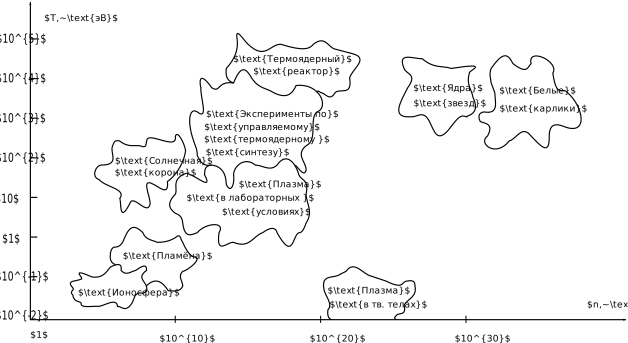
\includegraphics[width=0.95\textwidth]{Chapter_5/v5_0.pdf}
	\caption{Различные типы плазмы в лаборатории и природе. Температура
    дана в энергетических единицах ($1\;эВ\approx 11\,600\;К$)}
	\figmark{Types of plasma}
\end{figure}

Свойствами, характерными для газовой плазмы, обладают и некоторые другие среды,
называемые по этой причине
\emph{плазмоподобными} средами, или просто плазмами: в этом смысле термин
\important{плазма} встречается в научной литературе во множественном числе.
В~качестве примеров различных плазм можно назвать плазму металлов,
электронно-дырочную плазму полупроводников, нуклонную плазму атомного ядра.
Различные типы плазм, встречающихся как в лабораторных условиях,
так и в природе, можно достаточно наглядно представить на плоскости параметров:
температура плазмы~--- плотность числа частиц (рис.~\figref{Types of plasma}).
% Под температурой плазмы в каждом конкретном случае понимают температуру тех
% заряженных частиц, которые определяют плазменные свойства рассматриваемой среды:
% в большинстве случаев это электроны.

\section{Основные свойства плазмы}

Определяющими свойствами плазмы являются коллективный характер её движения
и квазинейтральность (равенство нулю средней плотности заряда).
Рассмотрим простейший вид коллективных плазменных колебаний. Здесь и далее
в этом разделе будем использовать систему СГС, как это принято в физике плазмы.

\begin{figure}[h!]
    \psfrag{E}[cb]{$E$}
    \psfrag{0}[ct]{0}
    \psfrag{X}{$X$}
    \psfrag{x}[ct]{$x$}
    \centering
    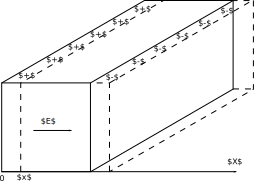
\includegraphics[width=0.3\textwidth]{Chapter_5/v5_1}
    \caption{Плазменные колебания}
    \figmark{1}
\end{figure}

\paragraph{Плазменная частота.}
Выделим в нейтральной плазме некоторый объём в виде параллелепипеда
(см. рис.~\figref{1}).
Обозначим концентрацию электронов как $n_e$; ионы для простоты будем считать
однозарядными ($Z=1$), тогда их концентрация такая же, как у электронов: $n_i=n_e$.
Предположим, что все электроны сместились на расстояние $x$ относительно ионов
(ионы как существенно более тяжёлые частицы можно считать неподвижными).
% (ионы занимают объём, изображённый сплошными, а электроны~--- пунктирными линиями).
В результате на гранях параллелепипеда возникнут нескомпенсированные
поверхностные заряды с плотностью
\begin{equation*}
%     \eqmark{5.13}
    \sigma = n_e e x.
\end{equation*}
Эти заряды --- как две пластины конденсатора --- создадут электрическое поле
\begin{equation*}
%     \eqmark{5.14}
    E=4\pi\sigma=4\pi n_e e x.
\end{equation*}
В свою очередь это поле будет действовать на электроны,
придавая им ускорение, равное
\begin{equation*}
%     \eqmark{5.15}
    \frac{d^2x}{dt^2}=-\frac{eE}{m}=-\frac{4\pi ne^2}{m}x.
\end{equation*}
Полученное уравнение описывает гармонические колебания с частотой
\begin{equation}
    \eqmark{5.16}
    \omega_p=\sqrt{\frac{4\pi n_e e^2}{m_e}}.
\end{equation}

Таким образом, мы получили частоту коллективных колебаний
электронов относительно квазинейтрального состояния. Такие колебания
называют \important{ленгмюровскими}, а частоту $\omega_p$ ---
\important{плазменной} или \important{ленгмюровской}. Эта частота ---
одна из важнейших характеристик плазмы.
Она задает естественный масштаб времени для плазмы: это~--- время
отклика на флуктуацию плотности заряда в плазме,
и определяет многие происходящие в ней процессы: от собственно плазменных
колебаний до распространения электромагнитных волн в ней.

% Для рассчётов можно использовать практическую формулу
% \begin{equation}
%     \eqmark{omegap-practical}
%  \omega_p =5,65\cdot10^4\sqrt{n[\text{см}^{-3}]}\;рад/с.
% \end{equation}

\paragraph{Дебаевский радиус.}
%  Учитывая это, дебаевский радиус экранирования можно интерпретировать
% следующим образом.
Плазменные колебания могут быть раскачены как с счёт внешнего воздействия
(например, при прохождении электромагнитной волны), так и за счёт
тепловой энергии, содержащейся непосредственно в плазме.
Оценим амплитуду колебаний электронов относительно ионов,
возникающих за счёт тепловых флуктуаций.

Пусть электроны колеблются с некоторой амплитудой $x_0$ и частотой $\omega_p$.
Тогда амплитуда их скорости равна $v_0 = \omega_p x_0$.
Полная энергия колебаний, как известно из механики,
равна максимальному значению кинетической энергии.
В расчёте на один электрон имеем энергию $W= \frac12 m_e \omega_p^2 x_0^2$.
С другой стороны, из термодинамики известно, что эта энергия должна
быть равна тепловой энергии, приходящейся на одну степень свободы
$W_Т = \frac12 \kB T_e$. Отсюда находим $x_0^2 = \frac{\kB T_e/m_e}{\omega_p^2}$.
Выразим с учётом \eqref{5.16} амплитуду колебаний и обозначим полученный
результат как
\begin{equation}
    \eqmark{5.17}
    r_D=\sqrt{\frac{\kB T_e}{4\pi n_e e^2}}.
\end{equation}
Величину $r_D$ называют \important{дебаевским радиусом}
(или \important{дебаевской длиной}).
Это ещё один важный плазменный параметр, задающий характерный масштаб
многих плазменных явлений.

Видно, что дебаевская длина есть амплитуда ленгмюровских колебаний,
возбуждаемых тепловыми флуктуациями. Она задаёт масштаб, на котором возможно
\emph{нарушение квазинейтральности} плазмы (в отсутствие внешнего поля).
Заметим также, что формулу \eqref{5.17} можно переписать как
\[
r_D = \frac{v_{Te}}{\omega_p},
\]
где $v_{Te}=\sqrt{\kB T_e/m_e}$~--- скорость, по порядку величины равная
средней тепловой скорости движения электронов.

Таким образом, плазменная частота $\omega_p$ и дебаевская длина $r_D$
есть две важнейшие характеристики плазмы, определяющие в том числе
временной и пространственный масштабы коллективного движения электронов
относительно ионов.

% Как следует из \eqref{5.16}, плазменная частота определяется только плотностью
% электронов (и универсальными постоянными).
% Можно строго доказать, что она не зависит от формы рассматриваемого возмущения и
% является, таким образом,
% локальной характеристикой плазмы. Плазменная частота является не
% единственной~--- но важнейшей~--- характерной частотой
% плазмы. Она определяет коллективное движение электронов относительно ионов.

\paragraph{Плазменное экранирование.}
Рассмотрим ещё одну задачу, в которой дебаевская длина играет роль
ключевого параметра.

Поместим в плазму с температурой $T$ некоторую пробную частицу, имеющую фиксированный
положительный $+q$ и найдём, как распределятся плазменные частицы вокруг неё.
Будем считать, что частица достаточно массивна, так что её можно
считать неподвижной (в качестве такого пробного заряда можно рассмотреть
и один из ионов плазмы, поскольку $m_i \gg m_e$).

Заряд будет притягивать к себе плазменные электроны, в результате чего
вокруг него образуется отрицательно заряженная <<подушка>>,
\emph{экранирующая} поле заряда на большом расстоянии от него ---
электрическое поле вокруг $q$ будет убывать с расстоянием $r$
не по закону $q/r^2$, а существенно быстрее.
Если бы электроны не имели кинетической энергии, то они так <<облепили>>
бы пробный заряд, что его собственное поле было бы полностью скомпенсировано.
Тепловое движение мешает такой компенсации.

Чтобы максимально наглядно выявить характерные особенности решения данной задачи,
предположим, что радиус $r_0$ пробной частицы велик (по сравнению с $r_D$)
и будем рассматривать распределение поля вблизи её поверхности ---
так мы сведём задачу к одномерной, сильно упростив выкладки, но не потеряв
качественные особенности решения.

% Как уже говорилось, во всяком сколько-нибудь большом объёме заряды ионов и электронов
% всегда практически компенсируют друг друга. Если хотя бы на некоторое
% время это оказывается не так, возникают сильные электрические поля,
% восстанавливающие квазинейтральность плазмы.
% Покажем, что именно дебаевская длина $r_D$ определяет размер области,
% внутри которой могут существовать заметные электрические
% поля и нарушаться квазинейтральность.

Пространственное распределение электронов в равновесии подчиняется
\emph{закону Больцмана}:
\begin{equation}
    \eqmark{5.5}
    n_e=n_{e0} \cdot \exp\left(\frac{e\varphi}{\kB T}\right)
\end{equation}
Здесь $\varphi$~--- потенциал электростатического поля,
$n_{e0}$ --- концентрация электронов вдали от заряда, где $\varphi\to 0$.
Аналогичное соотношение можно записать и для ионов с заменой $-e\to e$
(по-прежнему считаем, что $Z=1$).
% \begin{equation}
%     \eqmark{5.5}
%     n_i(r) \approx n_0 \left(1-\frac{e\varphi}{\kB T}\right).
% \end{equation}
Будем считать, что температура электронов в плазме достаточно велика, так что
можно положить
\[
e\varphi\ll \kB T.
\]
Раскладывая больцмановскую экспоненту в ряд по этому малому параметру,
найдём объёмную плотность заряда в плазме:
\begin{equation}
\eqmark{rho_ei}
\rho = -en_e + en_i \approx -(n_{e0}+n_{i0}) \frac{e\varphi}{\kB T}.
\end{equation}

С другой стороны, распределение потенциала $\varphi$ в пространстве
однозначно связано с распределением плотности электрического заряда~$\rho$.
Применяя \emph{теорему Гаусса} в дифференциальной форме
\[
\frac{dE}{dx}= 4\pi \rho,
\]
и пользуясь определением потенциала электростатического поля
$E = - \frac{d\varphi}{dx}$, получим
\begin{equation}
    \eqmark{poisson-1d}
    \frac{d^2\varphi}{dx^2} = - 4\pi \rho.
\end{equation}
Уравнение \eqref{poisson-1d} представляет собой частный (одномерный)
случай \emph{уравнения Пуассона}.

Объединяя \eqref{poisson-1d} и \eqref{rho_ei}, получим окончательно
дифференциальное уравнение на потенциал поля $\varphi(x)$ вблизи пробной частицы:
\begin{equation}
    \frac{d^2\varphi}{dx^2} = \frac{\varphi}{r_D^2},
\end{equation}
где $r_D$ определяется соотношением \eqref{5.17}, в котором вместо
$n_e$ стоит полная концентрация частиц в плазме $n=n_{e0}+n_{i0}$.
Решение, удовлетворяющее граничным условиям
$\varphi(\infty)=0$ и~$\varphi(0)=\frac{q}{r_0}$, есть%
\footnote{Решая уравнение Пуассона в сферических координатах,
можно показать, что для точечного пробного заряда
(в том числе, для отдельного иона) распределение потенциала будет
\[
\varphi(r) = \frac{q}{r} e^{-\tfrac{r}{r_D}}.
\]}
\begin{equation}
\varphi(x) = \frac{q}{r_0} e^{-\tfrac{x}{r_D}}.
\end{equation}

Таким образом, из полученного следует, что электрическое поле (и его потенциал),
а также концентрация плазменных частиц изменяются при удалении от
пробного заряда по экспоненциальному закону с характерной длиной порядка
дебаевского радиуса $r_D$. На расстояниях, превышающих $r_D$ в несколько раз,
плазму можно считать квазинейтральной, а поле заряда $q$ практически
полностью экранированным. В связи с этим дебаевскую длину также называют
\important{радиусом экранирования}.

% Формула для дебаевского радиуса \eqref{5.10} не учитывает движение ионов.
В заключение отметим одно обстоятельство, часто вводящее в заблуждение.
В общем случае неравновесной плазмы, когда температуры электронов~$T_e$
и ионов~$T_i$ различны, радиус экранирования \emph{стороннего заряда} будет определяться следующим
соотношением (предлагаем получить самостоятельно):
\begin{equation}
\eqmark{5.18}
r_{D} = \sqrt{\frac{\kB}{4\pi n_e e^2} \frac{T_i T_e}{T_i+T_e}}.
\end{equation}
то есть вместо $T_e$ в формулу для дебаевского радиуса войдёт <<приведённая>>
температура. В частности,
% при $T_e=T_i$ появляется множитель $\sqrt{2}$, а
при $T_e\gg T_i$ (например, в плазме газового разряда)
радиус экранирования стороннего заряда определяется температурой
холодных ионов~$T_i$. При этом стоит подчеркнуть, что рассуждения предыдущего параграфа, сделанные
при выводе \eqref{5.17}, остаются в силе и в случае $T_e\gg T_i$:
масштаб, на котором нарушается квазинейтральность из-за тепловых
флуктуаций электронов относительно ионов, определяется \emph{именно
формулой} \eqref{5.17}, то есть зависит от температуры электронов~$T_e$.
% Чтобы разделить эти два не всегда сопадающие понятия,
% выражение \eqref{5.17} иногда
% называют \important{электронной поляризационной длиной}.

% формуле \eqref{5.10}
% вместо $T_e$ будет стоять~$T_i$.

% Подставляя \eqref{5.5} и \eqref{5.6} в \eqref{5.4}, получим:
% \begin{equation}
% 	\eqmark{5.7}
% 	\frac{d^2\varphi}{dr^2}+\frac{2}{r}\frac{d\varphi}{dr}=-4\pi
% ne\left[1-e^{e\varphi/kT_e}\right].
% \end{equation}
%
% Это уравнение нелинейно и в аналитическом виде не решается. Решение может быть
% найдено, если считать, что:
% \begin{equation}
% 	\eqmark{5.8}
% 	\frac{e\varphi}{kT_e}\ll1.
% \end{equation}
%
% В этом случае экспоненту можно разложить в ряд и уравнение \eqref{5.7}
% становится линейным:
% \begin{equation}
% 	\eqmark{5.9}
% \frac{d^2\varphi}{dr^2}+\frac{2}{r}\frac{d\varphi}{dr}=\frac{1}{r_D^2}\varphi,
% \end{equation}
% где введено обозначение
% \begin{equation}
% 	\eqmark{5.10}
% 	r_D=\sqrt{\frac{kT_e}{4\pi
% ne^2}}=743\sqrt{\frac{T_e~(\text{эВ})}{n~(\text{см}^{-3})}}~(\text{см}).
% \end{equation}

% Это решение правильно ведёт себя около иона (где $\varphi\propto e/r$) и
% обращается в нуль на бесконечности. Мы нашли,
% следовательно, искомое решение задачи. Оно показывает, что вследствие
% экранирующего действия электронов поле иона
% убывает с расстоянием экспоненциально с характерной длиной, равной $r_D$~---
% дебаевскому радиусу
% (сам Дебай ввёл понятие радиуса экранирования, рассматривая поле иона в
% электролите). В связи с этим дебаевскую длину также называют
% \import{радиусом экранирования}.

% Таким образом, плазму можно считать почти нейтральной (квазинейтральной)
% в областях, размеры которых существенно превосходят дебаевскую длину.
% При $T=10^4$~К ($\approx 1$~эВ) и $n=10^9 ~\text{см}^{-3}$, $r_D\approx
% 1,6\cdot10^{-2}$~см.

\paragraph{Идеальная и неидеальная плазма.}
Теперь можно дать \emph{количественное} определение понятия плазма
(это определение также принадлежит Ленгмюру).

\important{Плазмой} называется \emph{ионизованный газ, дебаевский радиус которого
    $r_D$ существенно меньше характерного размера области $a$, занимаемой этим газом}:
\begin{equation*}
	\sqrt{\frac{kT_e}{4\pi ne^2}}\ll a.
\end{equation*}

Именно при $a\gg r_D$ поведение среды носит существенно коллективный характер.
В противном случае среда может рассматриваться как газ с примесью индивидуальных
заряженных частиц.

Оценим энергию кулоновского взаимодействия частиц в плазме.
Как показано выше, распределение потенциала вокруг иона с зарядом $q$
определяется законом экранирования
\[
\varphi = \frac{q}{r} e^{-r/r_D}.
\]
Вычитая потенциал самого иона $\varphi_0=\frac{q}{r}$, найдём
потенциал <<экранирующего облака>>. При $r\lesssim r_D$ имеем
\[
\varphi-\varphi_0 = \frac{q}{r}\left( e^{-r/r_D} - 1\right)
\approx - \frac{q}{r_D}.
\]
Воспользуемся известной формулой для электростатической энергии системы
зарядов $\varepsilon=\sum_i \varphi_i q_i$, где $\varphi_i$ --- потенциал
в точке нахождения заряда $q_i$. Суммируя по всем ионам,
найдём плотность энергии взаимодействия зарядов в плазме:
\begin{equation}
w_{кул} \approx -\frac12 n \frac{q^2}{r_D}.
\end{equation}

Сравним полученную энергию с тепловой $w_T \sim n \kB T$:
\begin{equation}
\frac{w_T}{w_{кул}} \sim
\frac{\kB T r_D}{q^2} \sim 4\pi n r_D^3.
\end{equation}
Видно, что отношение тепловой и кулоновской энергии в плазме по порядку величины
есть число частиц в сфере радиуса $r_D$:
\begin{equation}N_D = \frac43 \pi n r_D^3.
\end{equation}


Плазму называют \important{идеальной}, если энергия кулоновского взаимодействия
мала по сравнению с тепловой, что выполняется, если число частиц
в <<дебаевской сфере>> велико, $N_D\gg 1$. Идеальная плазма во многом подобна
по своим свойствам идеальному газу. В неидеальной плазме ($N_D\lesssim 1$)
взаимодействие между частицами велико, так что она становится в чём-то
подобна жидкости, а её описание значительно усложняется.

% Плазму можно
% Ещё одним важным параметром плазмы является число заряженных частиц (в среднем)
% в дебаевской сфере (сфера с радиусом,
% равным $r_D$). Применённый при выводе дебаевского радиуса статистический подход
% (распределение Больцмана) предполагает,
% что частиц должно быть много. Число частиц $N_D$ в дебаевской сфере можно
% оценить с помощью формулы \eqref{5.10},
% подставляя в неё вместо истинного среднее число частиц (эти величины мало
% различаются):
% \begin{equation}
% 	\eqmark{5.12}
% 	N_D\approx n\frac43\pi r_D^3\approx0,1\frac{(kT_e)^{3/2}}{n^{1/2}e^3}.
% \end{equation}
% Для плазмы газового разряда это число оказывается порядка $10^4$, т.~е. очень
% велико.

% В заключение заметим, что требование, чтобы число частиц в дебаевской сфере было велико по
% сравнению с единицей, эквивалентно
% условию, что потенциальная энергия взаимодействия двух заряженных частиц в
% плазме существенно меньше их тепловой
% энергии, то есть что плазма является газом, причём идеальным.

% Другой важнейшей характеристикой плазмы является \important{плазменная} или
% \important{ленгмюровская} частота, выражение для
% которой и её смысл можно получить из следующих соображений. Выделим в плазме
% объём в виде параллелепипеда, изображённого на рис.~\figref{1}.
%
% \begin{figure}[h!]
% 	\psfrag{E}[cb]{$E$}
% 	\psfrag{0}[ct]{0}
% 	\psfrag{X}{$X$}
% 	\psfrag{x}[ct]{$x$}
% 	\centering
% 	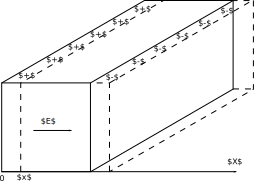
\includegraphics[width=0.3\textwidth]{Chapter_5/v5_1}
% 	\caption{???}
% 	\figmark{1}
% \end{figure}
%
% Сместим все электроны на расстояние $x$ относительно ионов (ионы занимают объём,
% изображённый сплошными, а
% электроны~--- пунктирными линиями).
% \todo[author = Andrew]{В картинке для нанесения некоторых обозначений был
% использован psfrag, который несовместим с pdf. Также отсутствует подпись к
% картинке. Необходимо исправить изображение.}
% Пусть плотность электронов (и ионов) равна $n$; ионы для простоты будем считать
% однозарядными. Легко видеть, что в результате такого смещения на гранях
% параллелепипеда возникнут поверхностные заряды:
% \begin{equation}
% 	\eqmark{5.13}
% 	\sigma=nex.
% \end{equation}
%
% Вследствие этого появится электрическое поле:
% \begin{equation}
% 	\eqmark{5.14}
% 	E=4\pi\sigma=4\pi nex.
% \end{equation}
%
% Это поле действует на электроны, придавая им ускорение, равное
% \begin{equation}
% 	\eqmark{5.15}
% 	\frac{d^2x}{dt^2}=-\frac{eE}{m}=-\frac{4\pi ne^2}{m}x.
% \end{equation}
%
% Уравнение \eqref{5.15} определяет плазменную (ленгмюровскую) частоту
% коллективных колебаний электронов:
% \begin{equation}
% 	\eqmark{5.16}
% 	\omega_p=\sqrt{\frac{4\pi n
% e^2}{m_e}}=5,65\cdot10^4\sqrt{n~(\text{см}^{-3})}.
% \end{equation}
%
% Плазменная частота задает естественный масштаб времени для плазмы: это~--- время
% отклика на флуктуацию плотности заряда в
% плазме. Учитывая это, дебаевский радиус экранирования можно интерпретировать
% следующим образом. Пусть какая-то группа
% электронов получила направленную скорость, равную тепловой: $v=\sqrt{kT_e/m_e}$.
% При этом, как легко можно убедиться,
% обращаясь к формулам \eqref{5.16}, \eqref{5.10}, за время, равное
% $\omega_p^{-1}$, эта группа электронов пройдёт в направлении
% полученной скорости до полной остановки расстояние, как раз равное дебаевской
% длине, то есть
% \begin{equation}
% 	\eqmark{5.17}
% 	r_D=\frac{v}{\omega_p}.
% \end{equation}
%
% Таким образом, дебаевская длина~--- это амплитуда ленгмюровских колебаний
% плазмы, возбуждаемых тепловыми флуктуациями.
% Эта амплитуда и является масштабом нарушения квазинейтральности плазмы в
% отсутствие внешнего поля.
%
% Как следует из \eqref{5.16}, плазменная частота определяется только плотностью
% электронов (и универсальными постоянными).
% Можно строго доказать, что она не зависит от формы рассматриваемого возмущения и
% является, таким образом,
% локальной характеристикой плазмы. Плазменная частота является не
% единственной~--- но важнейшей~--- характерной частотой
% плазмы. Она определяет коллективное движение электронов относительно ионов.

\section{Электропроводность плазмы}

Приложим к плазме электрическое поле с напряжённостью $\vec{E}$. Под его
действием приходят в движение как электроны, так и
ионы. Действующие на них силы мало отличаются друг от друга, а массы различаются
очень сильно. Основными носителями тока
являются поэтому электроны. Свободно двигаясь на пути свободного пробега,
электроны приобретают направленную (дрейфовую)
скорость. После очередного соударения скорость электрона может иметь самые
разные направления, так что среднее значение
этой скорости в начале пробега близко к нулю. В конце пробега оно равно
\begin{equation*}
	\vec{v}_\text{кон}=-\frac{e\lambda}{m_e\average{v_e}}\vec{E},
\end{equation*}
где $\lambda$~--- длина свободного пробега, а $\average{v_e}$~--- тепловая
скорость электрона, по сравнению с
которой дрейфовая скорость обычно мала. Среднее значение дрейфовой скорости
равно поэтому половине $v_\text{кон}$:
\begin{equation}
	\eqmark{5.19}
	v_\text{др}=\frac{e\lambda E}{2m_e\average{v_e}}.
\end{equation}

Средняя тепловая скорость $\average{v_e}$ определяется из обычной формулы:
\begin{equation}
	\eqmark{5.20}
	\average{v_e}=\sqrt{\frac{8kT_e}{\pi m_e}}.
\end{equation}

Объединяя эти формулы, найдём
\begin{equation}
	\eqmark{5.21}
	\vec{v}_\text{др}=-b\vec{E},
\end{equation}
где подвижность электронов $b$ равна
\begin{equation}
 	\eqmark{5.22}
	b=\frac{e\lambda}{2\sqrt{\frac{8m_e}{\pi} kT_e}}.
\end{equation}

Электропроводность плазмы $\sigma$ определяется совместным дрейфовым движением
всех электронов, так что
\begin{equation}
	\eqmark{5.23}
	\sigma=\frac{j}{E}=\frac{n_eev_{др}}{E}=neb=\frac{e^2\lambda
n_e}{2\sqrt{\frac{8m_e}{\pi} kT_ei}}.
\end{equation}

Полученная формула показывает, что электропроводность плазмы пропорциональна
концентрации электронов и уменьшается с
ростом температуры плазмы. Длина свободного пробега $\lambda$ в
слабоионизированной плазме определяется не столько
плотностью электронов $n_e$, сколько плотностью газа.

\section{Одиночный зонд}

Распределение электрического потенциала в плазме обычно определяют с помощью
зондов~--- небольших проводников, вводимых в
плазму. Как уже говорилось выше, метод зондов был разработан Ленгмюром в начале
двадцатых годов XX века.

Рассмотрим явления, происходящие при внесении в плазму уединённого
проводника~--- зонда. Пусть электрический потенциал
зонда вначале равен потенциалу той точки плазмы, в которую будет помещён зонд.
Поступающие на зонд токи электронов и
ионов в этом случае равны
\begin{equation}
	\eqmark{5.24}
	I_{e0}=\frac{n\average{v_e}}{4}eS,
\end{equation}

\begin{equation}
	\eqmark{5.25}
	I_{i0}=\frac{n\average{v_i}}{4}eS,
\end{equation}
\begin{wrapfigure}{o}{0.5\textwidth}
	\psfrag{x}{$X$}
	\psfrag{r}[tc]{$r_D$}
	\psfrag{f}[rb]{$\varphi(x)$}
	\psfrag{v}[cc]{$U_f$}
	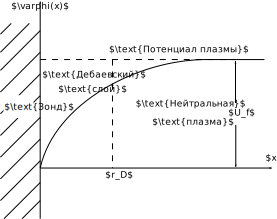
\includegraphics[width=0.5\textwidth]{Chapter_5/v5_8}
	\caption{Распределение потенциала в~окрестности зонда}
	\figmark{Potential distribution}
\end{wrapfigure}
\todo[author = Andrew]{В картинке для нанесения некоторых обозначений был
использован psfrag, который несовместим с pdf. Необходимо исправить
изображение.}
где $\average{v_e}$ и $\average{v_i}$~--- средние скорости электронов и ионов,
$S$~--- площадь зонда, $n$~--- плотность
электронов и ионов (которые в силу квазинейтральности плазмы равны или почти
равны друг другу). Множитель $\frac{1}{4}
n\average{v}$, согласно кинетической теории, определяет число ударов в секунду о
единицу поверхности. Так как скорости
электронов существенно превосходят скорости ионов, то $I_{e0}\gg I_{i0}$, так
что зонд заряжается до некоторого
отрицательного равновесного или, как обычно говорят, \important{плавающего}
потенциала~$-U_f$. При плавающем потенциале
количество попадающих на зонд ионов и электронов уравнивается, так как до него
могут доходить лишь наиболее быстрые
электроны и практически все ионы. Зонд, таким образом, приобретает отрицательный
заряд. Вокруг него образуется область
положительного пространственного заряда (её ширина по порядку величины равна
дебаевскому радиусу), экранирующего плазму
от зонда (рис.~\figref{Potential distribution}).

При установлении равновесия ионный ток мало меняется и в первом приближении
по-прежнему определяется формулой
\eqref{5.25}\footnote{Как мы увидим ниже, эта формула при $U\approx -U_f$ на
самом деле нуждается в поправках.}, а
выражение для электронного тока приобретает вид

\begin{equation}
	\eqmark{5.26}
	I_e=I_0\exp\left(-\frac{eU_f}{kT_e}\right),
\end{equation}
которое для плоских электродов следует из распределения Больцмана.

Возникновение <<дебаевского слоя>> вокруг зонда вносит некоторую
неоп-ределённость в величину $S$: становится неясно,
какая площадь должна подставляться в формулы~--- площадь зонда или площадь
поверхности этого слоя. При больших зондах
указанное различие несущественно, а при малых может оказаться важным.

Оценим величину плавающего потенциала. При равновесии электронный и ионный токи
равны друг другу:
\begin{equation*}
\frac{1}{4}n\average{v_i}eS=\frac{1}{4}n\average{v_e}eS\cdot
\exp\left(-\frac{eU_f}{kT_e}\right),
\end{equation*}
откуда
\begin{equation}
\eqmark{5.27}
eU_f=kT_e\ln\frac{\average{v_e}}{\average{v_i}}=
\frac12 kT_e\ln\frac{T_em_i}{T_im_e}.
\end{equation}

В тлеющем газовом разряде $kT_e\approx 1$~эВ, а $kT_i\approx \frac{1}{40}$~эВ
(комнатная температура). Положим для оценки
$m_i=10^4m_e$. Тогда
\begin{equation}
	\eqmark{5.28}
	eU_f%=\frac12\cdot 1~эВ\ln(40\.10^4)=
	\approx 6,5~\text{эВ}.
\end{equation}

Формулу \eqref{5.27} нельзя считать надёжной. При её выводе было сделано плохо
оправданное предположение, что движение
ионов близко к тепловому. Это справедливо вдали от дебаевского слоя, но не около
него и тем более не в нём, так как при
приближении к зонду дрейфовая скорость ионов быстро начинает превышать тепловую.
Формула для величины ионного тока при
этом должна быть изменена. Тем не менее для грубых оценок она может быть
использована.

Рис.~\figref{Potential distribution} иллюстрирует картину распределения
потенциала вокруг зонда.

\section{Исследование плазмы с~помощью одиночных~зондов}

При исследовании плазмы с помощью зондов на них подаются напряжения и
исследуются вольт-амперные
характеристики (ВАХ). Схема опытов изображена на \figref{Plasma study with
single probe}, на котором изображены два погружённых в плазму электрода и
источник $\mathcal{E}$, создающий между ними регулируемую разность потенциалов.
Пусть контактирующая с плазмой поверхность одного
электрода существенно меньше, чем у другого. Электрод с малой поверхностью будем
называть зондом, а электрод с большой
поверхностью~--- опорным электродом. Рассмотрим, как зависит ток $I_з$ в цепи
зонда от потенциала зонда~$U_з$
относительно опорного электрода.

\begin{figure}[h!]
	\centering
	\psfrag{I}[cc]{$I$}
	\psfrag{U}[cc]{$U$}
	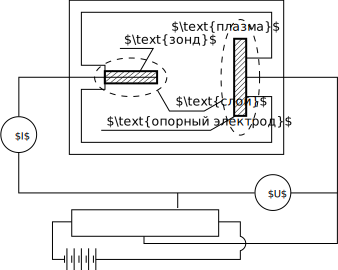
\includegraphics[width=0.7\textwidth]{Chapter_5/v5_9}
	\caption{К исследованию плазмы с~помощью одиночного~зонда}
	\figmark{Plasma study with single probe}
\end{figure}

Рассмотрим вначале случай, когда плазма эквипотенциальна. Пусть движок
потенциометра (рис.~\figref{Plasma study with single probe}) установлен так, что
зонд и
опорный электрод соединены накоротко. Ясно, что в этом случае они представляют
собой один электрод сложной формы,
внесённый в плазму.
\todo[author = Andrew]{В картинке для нанесения некоторых обозначений был
использован psfrag, который несовместим с pdf. Необходимо исправить
изображение.}
Зарядившись отрицательно, они принимают относительно плазмы потенциал, равный
плавающему потенциалу,
т.~е. $-U_f$. Полный ток на каждый электрод равен нулю, значит, электронный ток
равен ионному.

Если плазма не эквипотенциальна, то ток зонда обращается в нуль лишь в том
случае, если потенциалы зонда и опорного
электрода смещены на величину $U_f$ относительно потенциалов соответствующих
участков плазмы. Необходимая для этого
разность потенциалов между зондом и опорным электродом равна разности
потенциалов между соответствующими участками
плазмы. Измеряя потенциал зонда относительно опорного электрода (при нулевом
токе), можно исследовать распределение
потенциала в плазме.

Сведения о температуре и плотности зарядов в плазме получают, снимая
вольт-амперную характеристику зонда. Начнём
перемещать движок потенциометра (рис.~\figref{Plasma study with single probe}),
т.~е. подавать на зонд некоторый потенциал. Через плазму и по внешней цепи
начинает проходить ток, так как баланс между электронным и ионным током
нарушается. При этом
токи, проходящие через зонд и опорный электрод, конечно, равны друг другу, а
плотности тока различны, так как площади
электродов существенно различаются. Плотность тока, идущего через опорный
электрод, из-за большой площади последнего
всегда очень мала, и, следовательно, его потенциал относительно плазмы
практически всегда равен $-U_f$. При небольшом
размере зонда наибольшая плотность тока возникает около него, так что
практически всё падение напряжения приходится на
дебаевский слой, окружающий зонд.

Зависимость зондового тока $I_\text{з}$ от величины $U_\text{з}$ имеет вид,
показанный на рис.~\figref{Single probe VAC} (мы снова рассматриваем
эквипотенциальную плазму). Эта кривая носит название зондовой характеристики.
При $U_\text{з}<0$ весь ионный ток, приходящий на
границу дебаевского слоя, достигает зонда. Ионный ток равен, следовательно,
своему максимальному значению, или, как
говорят, ионному току насыщения $I_{i\text{н}}$.

\todo[author = Andrew]{В картинке для нанесения некоторых обозначений был
использован psfrag, который несовместим с pdf. Необходимо исправить
изображение.}
\begin{wrapfigure}{o}{0.5\textwidth}
	\psfrag{U}{$U_з$}
	\psfrag{I}[br]{$I_з$}
	\psfrag{0}[br]{0}
	\psfrag{a}[cr]{$I_{eн}-I_{iн}$}
	\psfrag{b}[cr]{$I_{eн}$}
	\psfrag{c}[cl]{$-I_{iн}$}
	\psfrag{d}[tc]{$U_f$}
	\psfrag{A}[rb]{$A$}
	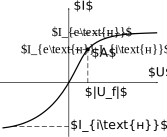
\includegraphics[width=0.5\textwidth]{Chapter_5/v5_10}
	\caption{Вольт-амперная характеристика одиночного~зонда}
	\figmark{Single probe VAC}
\end{wrapfigure}

При увеличении (по абсолютной величине) потенциала зонда электронный ток
уменьшается и, наконец, прекращается. Весь ток зонда является в этом случае
ионным током. На первый взгляд, величина
тока при этом не должна зависеть от потенциала зонда. На самом деле это не так,
поскольку при изменении потенциала
изменяется площадь поверхности дебаевского слоя и изменяются скорости ионов,
которые быстро увеличиваются при
перемещении из плазмы к электроду~--- от тепловых значений до значений,
определяемых величиной потенциала. Поэтому с
увеличением потенциала зонда (при смещении движка потенциометра влево на
рис.~\figref{Plasma study with single probe}) ток зонда возрастает, хотя и не
очень
сильно.

На правой ветви характеристики (при $U_\text{з}>0$) потенциал зонда превышает
потенциал опорного электрода, но вначале (вплоть
до точки $A$) остаётся ниже потенциала плазмы. При этом ионный ток на зонд не
меняется (вернее, слабо меняется), а
электронный ток возрастает. В точке $A$, т.~е. при $U_\text{з}=U_f$, слой
пространственного заряда (дебаевский слой) исчезает и
оба тока~--- электронный и ионный~--- подходят к зонду беспрепятственно. При
этом электронный ток, конечно, существенно
превосходит ионный, поскольку плотности электронов и ионов близки друг к другу,
а тепловые скорости существенно
различаются.

При дальнейшем увеличении $U_з$ ионный ток подавляется, а ток электронов не
изменяется и остаётся равным тепловому (на
самом деле, медленно возрастает по тем же причинам, по которым изменяется ионный
ток насыщения).

Участок характеристики, расположенный влево от точки $A$, носит название
\important{ионной} ветви (ионный ток равен току
насыщения), а участок вправо от точки $A$ называется \important{электронной}
ветвью вольт-амперной характеристики
(электронный ток равен току насыщения).

Оценим величину электронного и ионного тока насыщения. Электронный ток насыщения
определяется формулами \eqref{5.24},
\eqref{5.20}:
\begin{equation}
	\eqmark{5.29}
	I_{e\text{н}}=\frac14neS\average{v_e}\approx\frac14neS\sqrt{\frac{8kT_e}{\pi
m_e}}.
\end{equation}

Ионный ток насыщения по аналогичной формуле оценивать не следует, поскольку
скорости ионов в окрестности зонда
определяются не температурой плазмы, а разностью потенциалов между плазмой и
зондом:
\begin{equation}
	\eqmark{5.30}
	v_i\approx\sqrt{\frac{2eU}{m_i}}.
\end{equation}
Опыт показывает, что вместо формулы \eqref{5.29} для вычисления этого тока лучше
применять полуэмпирическую формулу,
предложенную Бомом:
\begin{equation}
	\eqmark{5.31}
	I_{i\text{н}}=0,4 neS\sqrt{\frac{2kT_e}{m_i}}.
\end{equation}

Структуру этой формулы нетрудно понять, замечая, что, согласно формуле
\eqref{5.27}, $U_f$ пропорционально $T_e$ (логарифмической
зависимостью $U_f$ при оценках следует пренебрегать). Численный коэффициент в
формуле \eqref{5.31} требует более подробных расчётов.

Вид выражения \eqref{5.31}, в которое входят температура электронов и масса
ионов, характерна для многих явлений в плазме.
Внешние поля приводят к быстрому перемещению электронов и к существенно более
медленному движению ионов. Значительное
перемещение электронов относительно ионов, однако, невозможно, так как оно
нарушило бы квазинейтральность плазмы.
Движение плазмы определяется поэтому массой ионов. В то же время перемещение
электронов существенно зависит как от
приложенных полей, так и от электронной температуры. Процессы, которые
определяются параметрами, одни из которых
характерны для электронов (в нашем случае~$T_e$), а другие~--- для ионов (в
рассматриваемой формуле~--- $m_i$), обычно
называются \important{амбиполярными}.

При измерениях с помощью одиночного зонда в качестве опорного электрода часто
используется анод газоразрядной трубки. Мы
уже отмечали, что падение напряжения в положительном столбе разряда невелико,
поэтому разности потенциалов, возникающие
между анодом и зондом, также оказываются небольшими и легко доступны измерениям.
Одиночные зонды используются для
исследования распределения потенциала в плазме, для измерения электронной
температуры и плотности электронов. Ещё лучше
делать это с помощью двойных зондов.

\section{Двойной зонд}

Двойным зондом называется система, состоящая из двух одинаковых зондов,
расположенных на небольшом расстоянии друг от
друга. Между зондами создаётся разность потенциалов, которая по величине много
меньше плавающего потенциала $U_f$. При
этом оба зонда имеют относительно плазмы близкий к плавающему отрицательный
потенциал, т.~е. находятся на ионной ветви
вольт-амперной характеристики.

При отсутствии разности потенциалов ток между зондами равен нулю. Рассчитаем
величину тока, проходящего через двойной
зонд вблизи точки $I=0$. При небольших разностях потенциалов ионные токи на оба
зонда равны ионному току насыщения и
компенсируют друг друга. Величина результирующего тока целиком связана с
различием в электронных токах. Пусть потенциал
на первом зонде равен
\begin{equation}
	\eqmark{5.32}
	U_1=-U_f+\Delta U_1,
\end{equation}
а на втором
\begin{equation}
	\eqmark{5.33}
	U_2=-U_f+\Delta U_2.
\end{equation}

По предположению $\Delta U_1$ и $\Delta U_2$ меньше $U_f$. Напряжение $U$ между
зондами равно
\begin{equation}
	\eqmark{5.34}
	U=U_2-U_1=\Delta U_2-\Delta U_1.
\end{equation}
Найдём ток, приходящий на первый электрод:

\begin{equation*}
	\begin{gathered}
I_1=I_{i\text{н}}+I_{e1}=I_{i\text{н}}-\frac{1}{4}neS\average{v_e}\cdot
\exp\left[\frac{e(-U_f+\Delta U_1)}{kT_e}\right]=  \\
	 	=
I_{i\text{н}}-\left\{\frac{1}{4}neS\average{v_e}\exp
\left(-\frac{eU_f}{kT_e}\right)\right\}
\exp\left(\frac{e\Delta U_1} {kT_e} \right).
	\end{gathered}
\end{equation*}

Заметим теперь, что при $\Delta U_1=0$ (при $U_1=U_f$) электронный и ионный ток
компенсируют друг друга. Это означает, что
заключённый в фигурные скобки множитель равен $I_{i\text{н}}$. Имеем поэтому
\begin{equation}
	\eqmark{5.35}
	I_1=I_{i\text{н}}\left[1-\exp\left(\frac{e\Delta U_1}{kT_e}\right)\right].
\end{equation}

Аналогично
\begin{equation}
	\eqmark{5.36}
	I_2=I_{i\text{н}}\left[1-\exp\left(\frac{e\Delta U_2}{kT_e}\right)\right].
\end{equation}

Заметим также, что зонды 1 и 2 соединены последовательно и через них проходит
один и тот же ток $I$, но в разном
направлении. Положим
\begin{equation}
	\eqmark{5.37}
	I_1=-I_2=I.
\end{equation}

Выразим $\Delta U_1$ и $\Delta U_2$ из \eqref{5.35} и \eqref{5.36} и заменим
входящие в эти выражения $I_1$ и $I_2$ через $I$ с
помощью \eqref{5.37}:
\begin{equation}
	\eqmark{5.38}
	\Delta U_1=\frac{kT_e}{e}\ln\left(1-\frac{I}{I_{i\text{н}}}\right),
\end{equation}

\begin{equation}
	\eqmark{5.39}
	\Delta U_2=\frac{kT_e}{e}\ln\left(1+\frac{I}{I_{i\text{н}}}\right).
\end{equation}

Вычитая второе равенство из первого, найдём
\begin{equation}
	\eqmark{5.40}
	U=\Delta U_1-\Delta
U_2=\frac{kT_e}{e}\ln\frac{1-I/I_{i\text{н}}}{1+I/I_{i\text{н}}}.
\end{equation}

Разрешая это равенство относительно $I$, найдём
\begin{equation}
	\eqmark{5.41}
	I=I_{i\text{н}}\th\frac{eU}{2kT_e}.
\end{equation}

Эта формула может служить для определения температуры электронов по форме
вольт-амперной характеристики двойного зонда.

Наблюдаемая на опыте зависимость тока от напряжения изображена на
рис.~\figref{Double probe VAC}. Эта кривая отличается от \eqref{5.41} наклоном
асимптот в области больших $|U|$. Этот наклон уже обсуждался в конце предыдущего
пункта. Наклон асимптот в первом приближении
является линейным. Поэтому вместо \eqref{5.41} лучше писать
\begin{equation}
	\eqmark{5.42}
	I=I_{i\text{н}}\th\frac{eU}{2kT_e}+AU,
\end{equation}
где $A$~--- некоторая константа, величина которой может быть найдена из опыта.

\todo[author = Andrew]{В картинке для нанесения некоторых обозначений был
использован psfrag, который несовместим с pdf. Необходимо исправить
изображение.}
\begin{wrapfigure}{o}{0.5\textwidth}
	\psfrag{U}{$U$}
	\psfrag{I}{$I$}
	\psfrag{0}[br]{0}
	\psfrag{1}[cr]{$I_{iн}$}
	\psfrag{2}[cl]{$-I_{iн}$}
	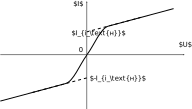
\includegraphics[width=0.5\textwidth]{Chapter_5/v5_11}
	\caption{Вольт-амперная характеристика двойного зонда}
	\figmark{Double probe VAC}
\end{wrapfigure}

Графики типа рис.~\figref{Double probe VAC} проще всего обрабатывать следующим
образом. Сначала находится $I_{i\text{н}}$ из пересечения асимптот
с осью $U=0$. Затем, по наклону асимптот, находится величина $A$. После этого из
\eqref{5.42} нетрудно определить $T_e$.
Дифференцируя эту формулу по $U$ в точке $U=0$ и принимая во внимание, что при
малых аргументах $\th\alpha\approx\alpha$,
а при малых наклонах кривой насыщения $A\to 0$, найдём
\begin{equation}
	\eqmark{5.43}
	kT_e=\frac12\frac{eI_{i\text{н}}}{\left.\frac{dI}{dU}\right|_{U=0}}.
\end{equation}

Концентрацию плазмы $n$ можно найти из формулы \eqref{5.31}. Как это уже ясно из
сказанного, двойные зонды удобно применять
для измерения электронной температуры и концентрации электронов в плазме.


\newpage

\lab{Изучение плазмы газового разряда в неоне}

\aim{изучение вольт-амперной характеристики тлеющего разряда; изучение свойств
плазмы методом зондовых характеристик.}

\equip{стеклянная газоразрядная трубка, наполненная изотопом неона,
высоковольтный источник питания, источник питания
постоянного тока, делитель напряжения, резистор, потенциометр, амперметры,
вольтметры, переключатели.}

Перед выполнением работы необходимо ознакомиться с разделами
\ref{sec:plasma}, \ref{sec:single} и \ref{sec:double} теоретического Введения
к разделу.
Подробное описание свойств тлеющего разряда можно найти в Приложении к разделу
(см. стр.~\pageref{sec:discharge}).

Схема установки для исследования плазмы газового разряда в неоне представлена на
рис.~\figref{Neon gas discharge}. Стеклянная газоразрядная
трубка имеет холодный (ненакаливаемый) полый катод, три анода и
\important{геттерный узел}~--- стеклянный баллон, на
внутреннюю поверхность которого напылена газопоглощающая плёнка
(\important{геттер}). Трубка наполнена изотопом неона
$^{22}$Ne при давлении 2~мм~рт. ст. Катод и один из анодов (I или II) с~помощью
переключателя $\text{П}_1$ подключаются через
балластный резистор~$R_\text{б}$ ($\sim500$ кОм) к~регулируемому высоковольтному
источнику питания (ВИП) с~выходным
напряжением до нескольких киловольт.

\begin{figure}[h!]
    \centering
    \footnotesize
	\pic{\textwidth}{Chapter_5/3_5_1}
	\caption{Схема установки для исследования газового разряда}
	\figmark{Neon gas discharge}
\end{figure}

При подключении к ВИП анода-I между ним и катодом возникает газовый разряд. Ток
разряда измеряется миллиамперметром
$A_1$, а падение напряжения на разрядной трубке~--- цифровым вольтметром
$V_{1}$, подключённым к трубке через
высокоомный (несколько десятков МОм) делитель напряжения с коэффициентом
$(R_1+R_2)/R_2$.

При подключении к ВИП анода-II разряд возникает в~проcтранстве между катодом и
анодом-II, где находится двойной зонд,
используемый для диагностики плазмы положительного столба. Зонды изготовлены из
молибденовой проволоки диаметром
$d$ и имеют длину~$l$. Они подключены к источнику питания через
потенциометр~$R$. Переключатель
$\text{П}_2$ позволяет изменять полярность напряжения на зондах. Величина
напряжения на зондах изменяется с~помощью дискретного
переключателя <<$V$>> выходного напряжения источника питания и потенциометра
$R$, а измеряется вольтметром~$V_2$. Для
измерения зондового тока используется микроамперметр~$A_2$.
Анод-III в нашей работе не используется.

\begin{lab:task}

\taskpreamble{В~работе предлагается снять вольт-амперную характеристику тлеющего разряда и
зондовые характеристики при разных токах
разряда и по результатам измерений рассчитать концентрацию и температуру
электронов в плазме, степень ионизации,
плазменную частоту и дебаевский радиус экранирования.}
    
\tasksection{Вольт-амперная характеристика разряда}

\item Установите переключатель~$\text{П}_1$ в положение <<Анод-I>> и подготовьте
приборы к работе согласно техническому описанию, которое находится в
лаборатории. Плавно увеличивая выходное напряжение ВИП, определите напряжение
зажигания разряда (показания вольтметра~$V_{1}$ перед зажиганием).

\item С помощью вольтметра~$V_{1}$ и амперметра~$A_{1}$ снимите вольт-амперную
характеристику разряда $U_{1}=f(I_\text{р})$. Ток разряда~$I_\text{р}$ изменяйте
в диапазоне, указанном в описании работы в лаборатории (при больших токах может
сгореть сопротивление).

\tasksection{Зондовые характеристики}

\item Уменьшите напряжение ВИП до нуля, переведите переключатель~$\text{П}_1$
в~положение <<Анод-II>> и подготовьте приборы~$\text{П}_{2}$, $V_{2}$ и~$A_{2}$
к работе согласно техническому описанию, которое находится в лаборатории.

\item Плавно увеличивайте напряжение ВИП до возникновения разряда. Установите
значение разрядного тока~$I_\text{р}$ согласно техническому описанию.
Подготовьте к работе источник питания. После этого при помощи
потенциометра~$R$ установите на зонде максимальное напряжение $U_{2 max}$.

\item Снимите вольт-амперную характеристику двойного зонда $I_{2}(U_{2})$
(в диапазоне от~$-U_{2 \rm max}$ до~$U_{2 \rm max}$) при фиксированном токе~$I_\text{p}$
согласно описанию работы в лаборатории.

\item Повторите измерения при другой полярности (переключатель~$\text{П}_2$).
Менять полярность подключения зондов можно только при \important{нулевом токе},
поддерживая при этом величину тока разряда~$I_\text{p}$ в трубке.

Записывая результаты в таблицу, одновременно стройте приближенный график
$I(U)$  в тетради в интервале от $-U_{2 \rm max}$ до~$U_{2 \rm max}$. Отцентрируйте
кривую: проведите ось абсцисс на уровне $I=\sum \Delta I/2$, восстановите ось
ординат из точки пересения кривой с новой осью абсцисс. Убедитесь, что можно
провести асимптоты к участкам кривой при больших напряжениях. Если точек мало~---
проведите дополнительные измерения.

\item Снимите зондовые характеристики при токах разряда, равных~3 и 1,5~мА.

\tasksection{Обработка результатов}

\item Постройте вольт-амперную характеристику разряда $U_{1}(I_\text{p})$.
По наклону кривой определите максимальное дифференциальное сопротивление разряда
$R_{\rm max}$.

\item Постройте семейство зондовых характеристик $I(U)$ на одном листе.

\item По зондовым характеристикам определите температуру электронов~$T_{e}$ по
формуле \chaptereqref{5.43}: ток $I_{i\text{н}}$ найдите из пересечения
асимптоты к току насыщения с осью $U=0$; ($dI/dU)|_{U=0}$~--- наклон
характеристики~$I(U)$ в точке $U=0$, $I=0$; рассчитайте
тепловую энергию электронов $\kB T_{e}$ в электрон-вольтах.

\item Полагая концентрацию электронов $n_{e}$ равной концентрации ионов $n_{i}$,
определите её из формулы \chaptereqref{5.31}:
\begin{equation*}
	I_{i\text{н}}=0,4n_{i}eS\sqrt{\frac{2\kB T_{e}}{m_{i}}}.
\end{equation*}
Здесь $S\approx \pi d l$~--- площадь поверхности зонда (в пренебрежении
дебаевским слоем); значения $d$ и $l$
приведены в описании экспериментальной установки.

\item Постройте графики зависимостей электронной температуры и
концентрации электронов от тока разряда $T_e(I_p)$, $n_e(I_p)$.

\item Рассчитайте плазменную частоту колебаний электронов по формуле
\chaptereqref{plasma-freq}.
% \begin{equation}
% 	\omega_{p}=\sqrt{\frac{n_{e} e^2}{\varepsilon_{0} m_{e}} }.
% \end{equation}

\item Рассчитайте дебаевский радиус экранирования~$r_{D}$ по формуле
\chaptereqref{debye-general},
которая в случае $T_{e}\gg T_{i}$ принимает вид
\begin{equation*}
	r_{D}=\sqrt{\frac{\kB T_{i}}{4\pi ne^{2}}}.
\end{equation*}
Сравните ответ с электронным дебаевским радиусом $r_{De}$
из формулы \chaptereqref{debye-rad}. Какие процессы характеризует каждая
из этих величин?

\item Оцените среднее число ионов в дебаевской сфере по формуле:
\begin{equation*}
	N_{D}=\frac{4\pi}{3} n_{i}r_{D}^{3}.
\end{equation*}
Является ли плазма разряда идеальной?

\item Оцените степень ионизации плазмы~$\alpha$ (долю ионизованных атомов),
если давление в трубке $p\simeq 1$~мбар.

\item Оцените погрешности эксперимента.

\end{lab:task}


\begin{lab:questions}
    \item Назовите различные виды плазм в лаборатории, приложениях и природе.
    
    \item Что такое дебаевский радиус экранирования?
    
    \item Дайте количественное определение понятия \term{плазма}.
    
    \item Что такое плазменная частота? Выведите формулу для плазменной частоты.
    Какие процессы в плазме характеризуются плазменной частотой?
    
    \item Чем определяется потенциал зонда, погружённого в плазму?
    
    \item Чем определяется зондовый ток насыщения для одиночного зонда? Для двойного
    зонда?
    
    \item Что такое равновесная и неравновесная плазма? 
    Является ли исследуемая в работе плазма равновесной?
    
    \item Опишите основной механизм зажигания тлеющего разряда.    
\end{lab:questions}



\lab{Индукционный газовый разряд}

%Я компилировала файл в Preamble.tex (сбросила его вместе со всеми файлами). При исправлении этой лабы опиралась на работу с магнитометром. Поэтому сейчас в PDF-формате сначала видно 
%Глава 1
%5
%Работа 3.1 (и далее название этой лабы)
%Таким образом, номер главы и номер лабы неверные.

%Также, в работе ниже стоят комментарии около всех формул из теоретического минимума (или введения), который обычно пишется перед лабами с близкими темами. Все номера формул закомментированы и записаны под тем номером, который у них сейчас в лабнике.

%Номер рисунка не читается. В PDF-файле около него стоят ??. Есть комментарий ниже.

%Контрольные вопросы так же стоят после теоретического минимума. В этой лабе и лабе 3.5.2 их не было. Тем не менее, можно в эти лабы добавить вопросы 1, 3--5, 7.

\begin{lab:aim}
{изучение свойств плазмы методом зондовых характеристик.}
\end{lab:aim}

\begin{lab:equipment}{газоразрядная трубка с высокочастотным (ВЧ)-генератором, источник постоянного тока, генератор звуковой частоты
(ЗГ), осциллограф (ЭО), форвакуумный насос, вакуумметр, натекатель, вакуумный кран, делитель (Д), повторители--фазовращатели --- нерегулируемый (ПФ1) и регулируемый (ПФ2).}
\end{lab:equipment}

% Первая строчка ``Оборудования'' каким-то образом в pdf вылезла на поля справа.

Газоразрядную плазму можно получить, используя электрические разряды в переменных высокочастотных (ВЧ) полях. Существуют
различные способы введения ВЧ-поля в разрядный объём. Один из них основан на использовании электромагнитной индукции:
через катушку-соленоид, в которую вставлена диэлектрическая газоразрядная камера, пропускается ток высокой частоты, и
внутри катушки индуцируется вихревое электрическое поле. Силовые линии этого поля, а вместе с~ними линии разрядного
тока, представляют собой замкнутые окружности. Такой разряд называется кольцевым, индукционным или разрядом $H$-типа,
что указывает на определяющую роль магнитного поля. Именно такой способ возбуждения газового разряда используется в нашей
установке.

\experiment
Схема установки представлена на рис. \ref{fig:gazovyj} % номер рисунка не виден после компиляции
. Заполненная газом диэлектрическая камера представляет собой цилиндрическую
стеклянную трубку (ее диаметр и длина указаны в описании), на одном из торцов которой впаяны две молибденовые проволочки (зонды)
диаметром~$d$ и длиной~$l$, расположенные на некотором расстоянии друг от друга. Другой конец трубки не запаян.
Он служит для откачки и для заполнения камеры газом. Трубка вставлена в катушку индуктивности колебательного контура
ВЧ-генератора, работающего на частоте~$\sim10$~МГц. Камера откачивается форвакуумным насосом и с помощью натекателя
заполняется воздухом до давления, указанного в описании работы в лаборатории. Значение давления контролируется вакуумметром
(термопарным манометром).

%\fcpic[1]{5_3_1}{Схема установки для исследования газового разряда}{1}
%\begin{wrapfigure}{r}{0.4\textwidth}
%	\pic{0.38\textwidth}{1_1_1}
%	\caption{Схема установки для исследования газового разряда}
%	\figmark[пфящмно]
%\end{wrapfigure}

\begin{figure}{c}
	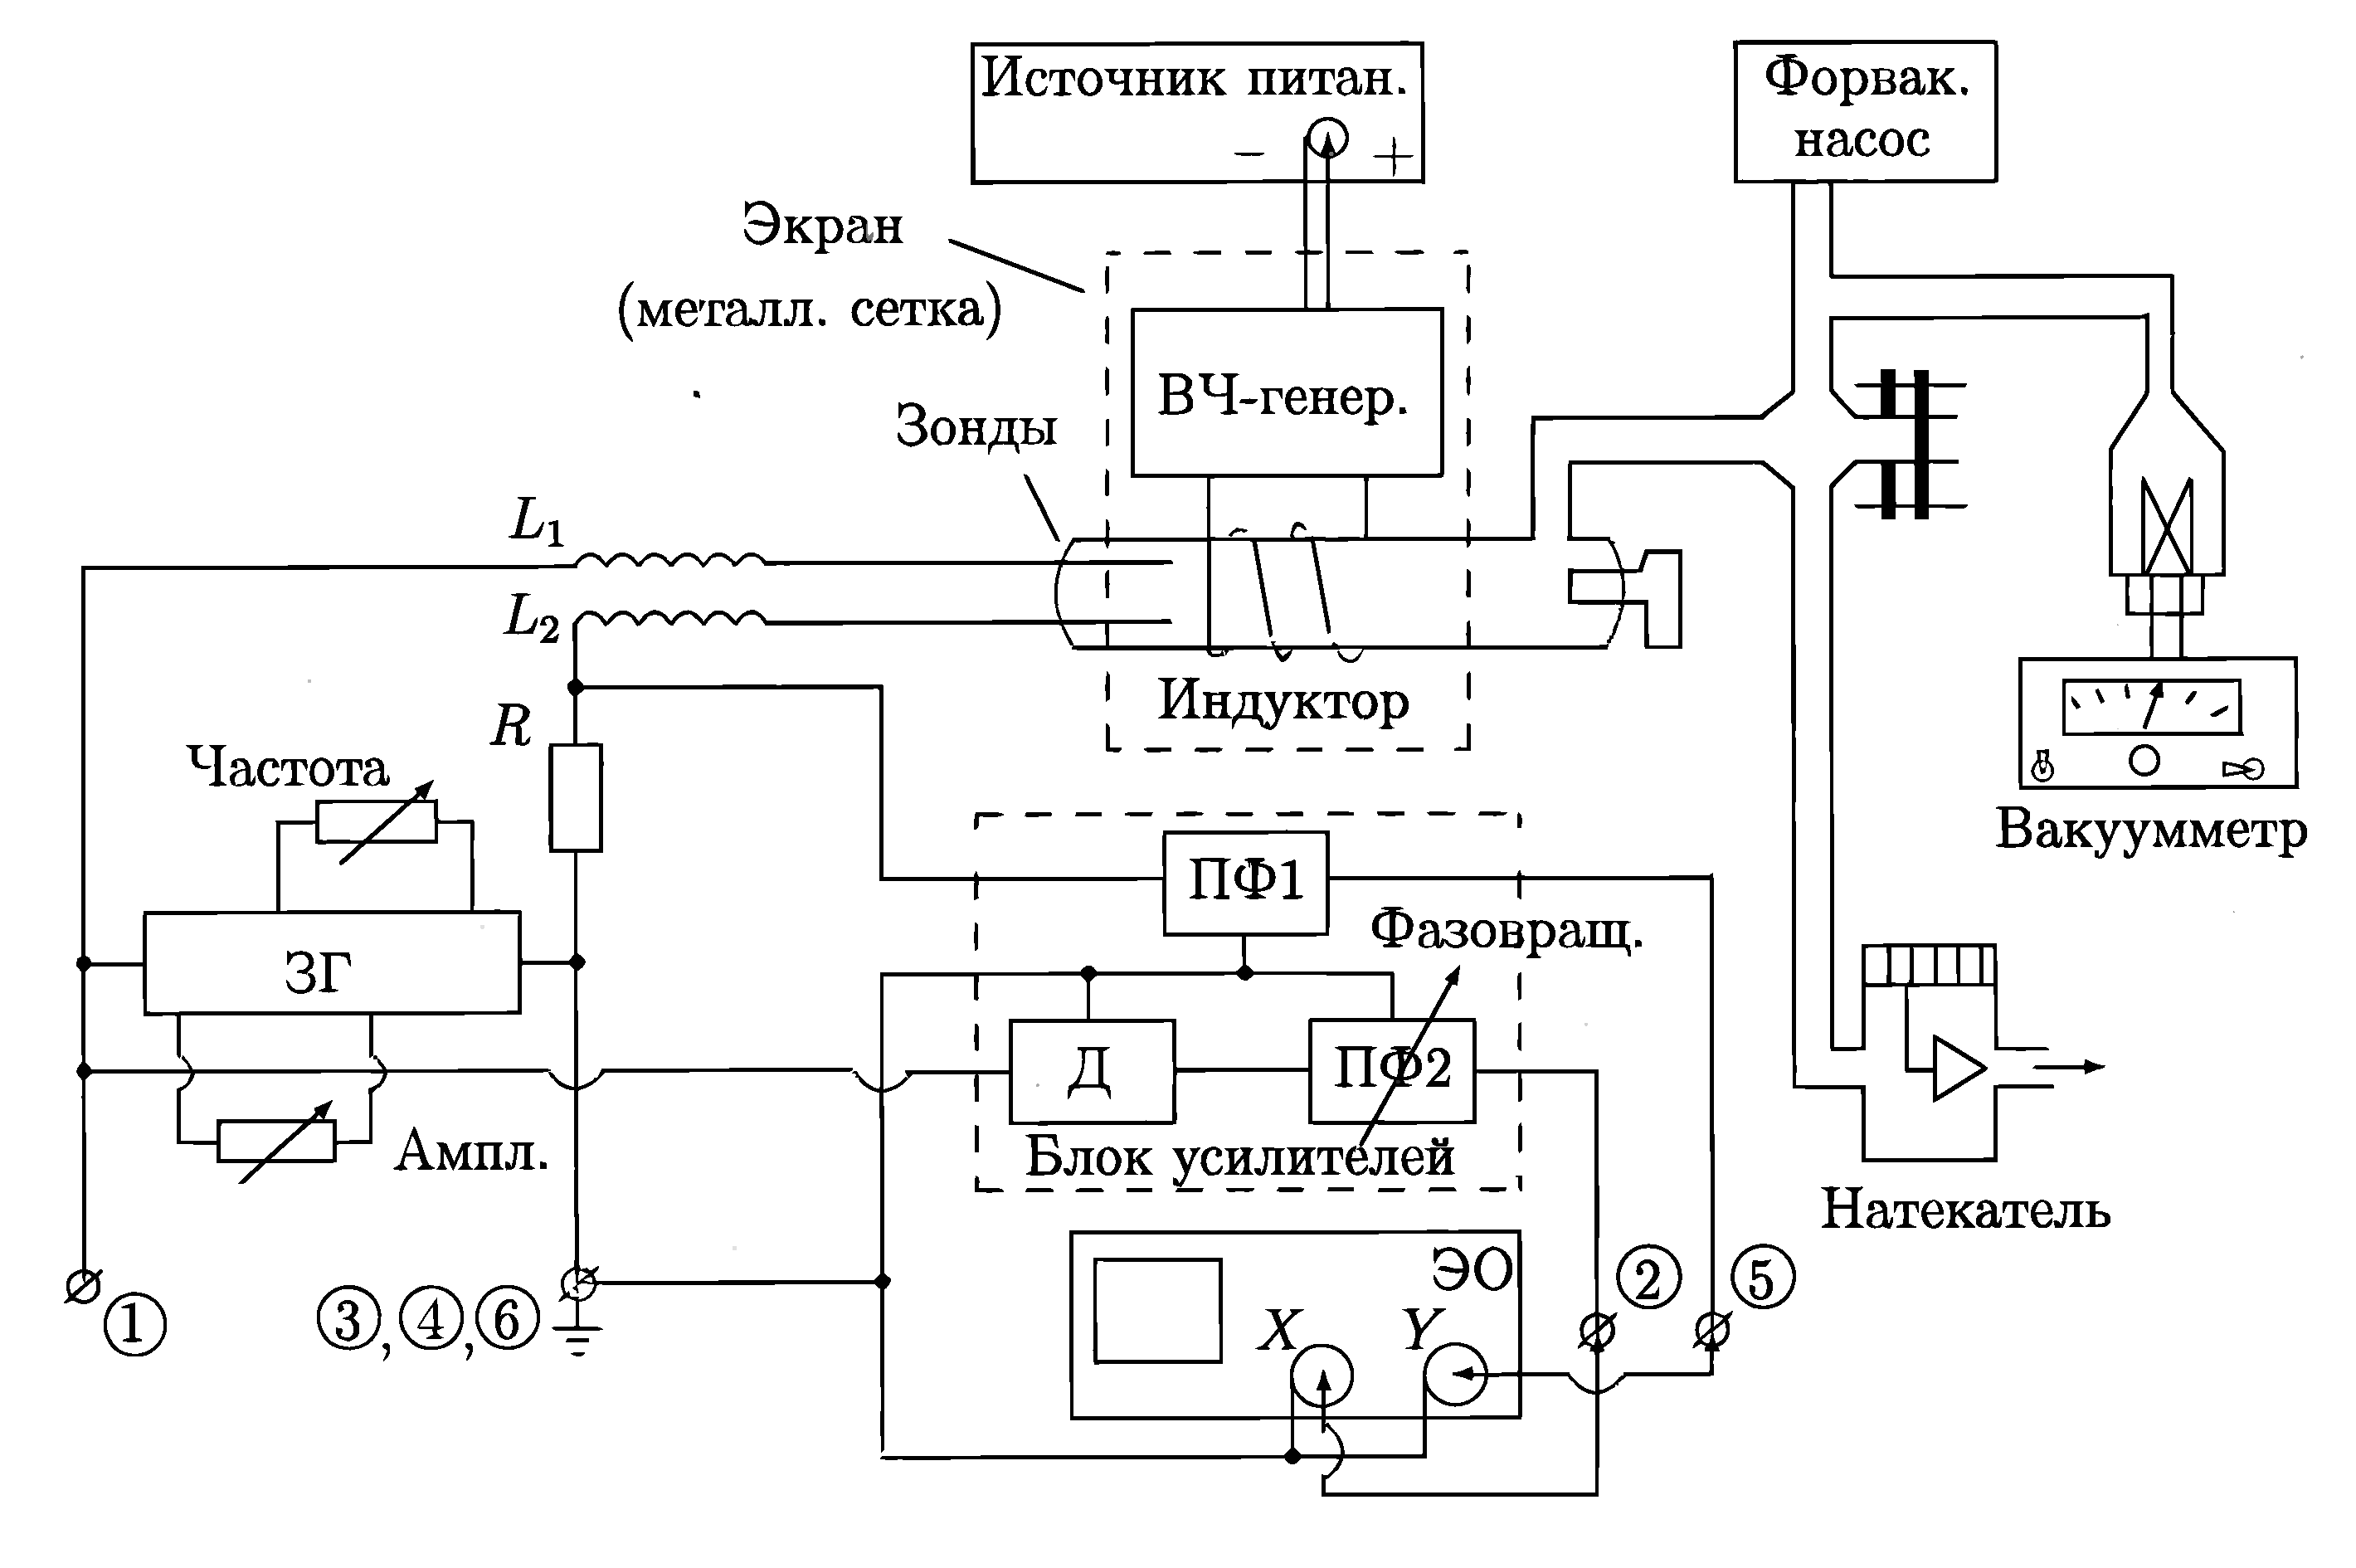
\includegraphics[width=120mm]{Chapter_5/3_5_2.eps}
	\caption{Схема установки для исследования газового разряда}
	\figmark[gazovyj]
\end{figure}

%Когда я компилирую файл с eps, то в левом нижнем углу вылазит буква ``с'' (отдельно от схемы). При просмотре eps и png никакой буквы ``с'' там нет. Появляется только после компиляции.

Следует отметить некоторые особенности процедуры установки рабочего давления в разрядной камере. Установка требуемого давления осуществляется путем изменения проходного сечения натекателя, соединенного с атмосферой, при непрерывной работе откачивающего насоса. При этом скорость откачки сохраняется постоянной, а приток воздуха в разрядную камеру определяется изменением аэродинамического сопротивления нагревателя. Таким образом, устанавливается новое значение давления, при котором скорость откачки насоса уравновешивается расходом воздуха через натекатель.

Изменение сечения натекателя выполняется микрометрическим винтом, который сжимает расположенную под ним пружину и изменяет ее давление на подвижную мембрану клапана. Такая система обладает очень большой инерциальностью и реагирует на вращение винта со значительным запозданием.
 
На зонды поступает синусоидальное напряжение от звукового генератора~ЗГ. Это же напряжение через делитель Д и регулируемый повторитель--фазовращатель ПФ2
подаётся на вход~$X$ осциллографа ЭО. Последовательно с зондом подключен датчик тока - резистор $R$ (значение сопротивления указано в описании работы). Напряжение, пропорциональное току, текущему через плазму, подаётся на вход~$Y$ ЭО через нерегулируемый повторитель-фазовращатель ПФ1. Две катушки $L_{1}$  и $L_{2}$, подключённые к~зондам, не пропускают на осциллограф высокочастотный сигнал. 

На
экране осциллографа наблюдается кривая, представляющая собой вольт-амперную характеристику двойного зонда (см.
рис.~% (5.12) из настоящего лабника \figref{v5_r6}
). Следует отметить, что на некоторых частотах в~измерительной цепи могут возникать фазовые сдвиги, и
характеристика зондов приобретает вид петли. Такие частоты для измерений непригодны. Для устранения фазовых сдвигов используется регулятор фазовращателя ПФ2.  



\begin{lab:task}

В работе предлагается при различных давлениях газа в~трубке получить зондовые вольт-амперные характеристики на экране
осциллографа и рассчитать с~их помощью температуру и~концентрацию электронов в~плазме, степень ионизации, плазменную
частоту и дебаевский радиус экранирования.

\subsection*{Подготовка приборов к работе}

\begin{enumerate}
\item Не включания приборов, ознакомьтесь с установкой (см. описание в лаборатории). 

\item Перед откачкой ознакомьтесь с техническим описанием вакууметра, расположенного на установке, и подготовьте его для работы. Включите форвакуумный насос и вакуумметр. Откачайте трубку до давления, указанного в описании работы в лаборатории. Давление
регулируется с~помощью натекателя (микровентиля) при постоянной откачке.

\item Включите источник питания ВЧ-генератора и проследите за разрядом в трубке: после зажигания разряд должен устойчиво
гореть по всей трубке, включая область расположения зондов.


\item  Включите осциллограф и звуковой генератор, при этом на зонды подается переменное напряжение от ЗГ с частотой, указанной в описании в лаборатории. Подберите напряжение, при котором на экране осциллографа должна появиться кривая, похожая на теоретическую зависимость, изображённую на рис. % рисунок (5.12) настоящего лабника)~\figref{v5_r11}.
Если на кривой не наблюдаются области насыщения, следует увеличить выходное напряжение~ЗГ. Если вместо кривой на экране
возникает петля, ее следует изменить регулировкой фазовращателя.

\item Посмотрите, как ведёт себя разряд, насколько он устойчив при изменении давления в
рабочем диапазоне. Отметьте, в какой области давлений наблюдаемая на экране кривая соответствует
теоретической.
\end{enumerate}

\subsection*{Измерения}

\begin{enumerate}
\item Получите на экране осциллографа вольт-амперную характеристику зондов (см. рис.~%рис.(5.12) настоящего лабника)\eqref{v5_r6}
) для максимального давления из выбранного диапазона.

\item Убедитесь, что ручка плавной регулировки усиления по осям~$X$ и $Y$ выведены вправо до щелчка (при таком положении ручки
чувствительность каналов соответствует величине, указанной возле искретного переключателя усиления). Регулируя напряжение звукового
генератора, добейтесь того, чтобы кривая занимала почти весь экран. При чрезмерно большом напряжении генератора возникает искажение зондовой характеристики, в ее оконечных областях появляются изломы и выпучины. Это происходит вследствие влияния электрического поля зондов на характер плазменного разряда. Такого допускать не следует, уменьшая при необходимости напряжение питания зондов до исчезновения искажений.

\item Зарисуйте кривую с~экрана на кальку. Укажите на
кальке давление (в мВ и м рт.ст.) и чувствительность осциллографа по осям $X$ и $Y$.

\item Повторите измерения п.~6 раздела ``Подготовка приборов к работе'' для 3--4-х давлений внутри интервала, выбранного Вами в п.~5 того же раздела.

\item Закончив работу, выключите сначала насос и немедленно откройте натекатель, затем отключите вакууметр и остальные приборы.

\end{enumerate}

\subsection*{Обработка результатов}

\begin{enumerate}

\item Для каждой кривой пересчитайте масштаб по оси~$Y$ из В/см в А/см, зная сопротивление, с которого сигнал,
пропорциональный зондовому току, подавался на ось~$Y$ осциллографа.

\item Рассчитайте масштаб по оси~$X$ в~В/см с учётом наличия делителя в канале зандового напряжения.

\item По зондовым характеристикам определите температуру~$T_e$ электронов по формуле %(5.43) настоящего лабника \eqref{v5_040}
: ток~$I_{iн}$ %в этом месте буква н в индексе русская, и она не видна после компиляции
найдите
из пересечения асимптоты к~току насыщения с~осью $U=0$ (см. рис.~%(5.12) настоящего лабника \eqref{v5_r11}
); $(dI/dU)|_{u=0}$~--- наклон
характеристики $I=f(U)$ в~точке $U=0$, $I=0$; взяв $\Delta U$ в~вольтах и приняв заряд электрона $e=1$, определите
энергию (<<температуру>>) электронов~$kT_e$ в~электрон-вольтах.

\item Концентрацию электронов $n_e$ определите из формулы (%(5.43) настоящего лабника \eqref{v5_040})\oref{v5_028}
), в которую вместо $n$ следует подставить $n_e$:
\begin{equation}
I_{iн}=0,4n_e eS\sqrt{\frac{2kT_e}{m_i}}.
\end{equation}
Здесь $S=\pi\cdot d\cdot l$~--- площадь поверхности зонда; значения $d$ и $l$ приведены в описании экспериментальной
установки; $m_i=14\cdot 1,66\cdot 10^{-24}$~г~--- масса иона азота.

\item Рассчитайте плазменную частоту колебаний электронов:
\begin{equation}
\omega_p=\sqrt{\frac{n_e e^2}{\epsilon_0 m_e}}.
\end{equation}

\item Рассчитайте дебаевский радиус~$r_{D}$ экранирования по формуле%(5.18) настоящего лабника \eqref{v5_5l})
, которая в случае $T_{e} \gg T_{i}$ принимает вид:
\begin{equation}
r_{D}=\sqrt{\frac{\epsilon_{0}kT_{i}}{n e^{2}}}.
\end{equation}

\item Оцените среднее число ионов в дебаевской сфере по формуле %(5.12) настоящего лабника \eqref{v5_41l})
.

\item Оцените степень ионизации плазмы (долю ионизованных атомов~$\alpha$), если давление в трубке $p \simeq1$~мбар.

\item Оцените погрешности.

\end{enumerate}

\end{lab:task}

\newpage

\labsupplement[Газовый разряд]

\begingroup
\small

\label{sec:discharge}

Под термином <<газовый разряд>> обычно понимают все явления и процессы,
связанные с протеканием электрического тока через газ.

Само название <<разряд>> произошло от названия медленно протекающего
процесса потери заряда заряженными металлическими телами,
расположенными на подставке из изолятора, что наблюдалось ещё в
XVI~веке. Позднее Кулон экспериментально доказал, что заряд стекает
с проводника через воздух, а не через подставку из изолятора.
Разряд при низких давлениях воздуха (порядка 1~мбар) открыл и исследовал
Фарадей~--- этот разряд стал известен как \term{тлеющий}. В конце XIX~века
исследование проводимости разреженных газов привело Дж.Дж.~Томсона к
открытию первой элементарной частицы~--- электрона, а дальнейшие исследования
физики газового разряда во многом послужили экспериментальной основой
атомной и квантовой физики.

% Основателем физики собственно газового разряда считается Таунсенд, ученик
% Дж.~Дж.~Томсона, создавший в начале XX~века
% теорию пробоя газа и установивший закономерности ионизации. Следующий
% принципиальный вклад в физику газового разряда был
% внесён Ленгмюром, который вместе с Тонксом в 1928~году, исследуя газовый разряд
% низкого давления, ввёл такое
% фундаментальное понятие физики, как плазма,
% а также развил методы исследования плазмы, в частности, метод зондов.

Современная физика термин \term{газовый разряд} трактует в более широком
смысле. Это~--- не только процесс протекания тока через газ, но и любой процесс
возникновения ионизации газа под действием приложенного электрического поля.
При этом поле может быть не только постоянным во времени,
но и переменным~--- высокочастотным (ВЧ-разряд, мегагерцы),
сверхвысокочастотным (СВЧ-разряд, гигагерцы) и даже оптического диапазона
(оптический разряд). Отдельно можно отметить пучково-плазменный разряд (ППР),
загорающийся при прохождении электронного пучка через газ малой плотности
вследствие возникновения в такой системе плазменных колебаний СВЧ-диапазона.
% Термины \important{горение} и \important{зажигание} получили распространение
% применительно к газовому разряду, потому что при достаточно сильной ионизации
% газ светится.

Разряды в постоянном поле разделяют на \term{несамостоятельные} и
\term{самостоятельные}. Дело в том, что при нормальных
условиях газы состоят в основном из электрически нейтральных атомов и
молекул и практически не проводят ток.
Проводниками могут быть только хоть в какой-то мере ионизованные газы.
Носителями тока в газах в могут быть положительные и отрицательные ионы и электроны.
Ионы могут возникать в результате действия различных
источников энергии, например: ультрафиолетового или рентгеновского излучения,
космических лучей, столкновений атомов газа с электронами и другими частицами, энергия
которых превышает потенциал ионизации атомов газа.

\subsection*{Несамостоятельный разряд и электронные лавины}
Предположим, что ионы в газовом проводнике создаются исключительно внешним
источником. Тогда при прекращении действия этого <<ионизатора>> ток и,
следовательно, разряд прекращаются.

Типичная кривая, отображающая связь между током через газовый промежуток и
напряжением на нём для \emph{несамостоятельного} разряда показана на
рис.~\figref{Non-self discharge VAC}. С повышением напряжения
на газовом промежутке ток сначала возрастает (кривая ОА), а потом достигает
насыщения и остаётся практически постоянным (участок АБ), что соответствует
полному вытягиванию на электроды зарядов, создаваемых внешним ионизатором.

\begin{figure}[h]
    \centering
    \pic{0.4\textwidth}{Chapter_5/v5_2}
    \caption{Вольт-амперная характеристика несамостоятельного газового разряда}
    \figmark{Non-self discharge VAC}
\end{figure}

\begin{figure}[h]
    \centering
    \pic{}{Chapter_5/v5-avalanche}
    \caption{Схема образования электронной лавины}
    \figmark{avalanche}
\end{figure}

При дальнейшем повышении напряжения ток снова начинает возрастать (участок БВ).
Это значит, что имеющиеся ионы, и прежде всего электроны, за период между двумя
последовательными столкновениями набирают такую энергию, что возникнет
\important{столкновительная ионизация}, то есть рождение новых 
(\important{вторичных}) ионов: $e^{-}+a\to i^{+} + 2 e^{-}$. При этом,
если количество выбитых при столкновениях электронов достаточно велико,
возникают и развиваются \term{электронные лавины},
то есть происходит <<размножение>> носителей и усиление тока,
часто называемое \term{газовым усилением} (см. рис.~\figref{avalanche}).
% При каком значении поля наступит размножение, зависит от давления
% газа и энергии, необходимой для ионизации
% данной молекулы (потенциала ионизации).
% В результате усиления концентрация ионов возрастает до величины, которая линейно
% или даже более сильно зависит от первичной ионизации.
При этом разряд остаётся несамостоятельным --- если убрать первичный источник
ионизации, пропадут и лавины.



В достаточно сильном электрическом поле проводимость газа может возрасти
скачком~--- возникает \term{пробой}.
% Соответствующее напряжение на газовом промежутке называется
% \term{напряжением пробоя} ( или \important{напряжением зажигания}).
Если после возникновения пробоя убрать внешний ионизатор, то разряд не
прекращается. Разряд переходит в режим \term{самостоятельного разряда}:
ионизация поддерживается процессами в самом разряде.

\subsection*{Критерий Таунсенда зажигания разряда}
Рассмотрим модель перехода несамостоятельного разряда в самостоятельный,
предложенную Таунсендом.
Определим \term{коэффициент объёмной ионизации} $\alpha$ ---
количество вторичных электронно-ионных пар, образуемых одним электроном
на единице длины пути.
Этот коэффициент зависит от плотности газа
(плотность определяет число соударений)
% растёт с увеличением давления $P$ газа
и растёт с увеличением напряжённости электрического поля $E$
(так как при этом увеличивается энергия электронов).
% , $\alpha=\alpha(P,\,E)$.

Рассмотрим, как происходит ионизация в газовом промежутке между плоскими
электродами~--- катодом и анодом (рис.~\figref{Townsend criterion}). На
расстоянии~$x$ от катода в слое толщины $dx$ один электрон создаёт $\alpha dx$
пар ионов. Если со стороны катода в этот
слой втекает электронный ток~$I_e$, то в слое он возрастёт на величину
\begin{equation}
\eqmark{dIx}
dI_e=I_e\alpha dx.
\end{equation}
Предположим, что токи в системе достаточно малы, так что в газовом промежутке
не накапливаются существенные объёмные заряды --- тогда электрическое поле~$E$,
а следовательно и коэффициент~$\alpha$, не зависят от~$x$
(это справедливво при малых токах, когда в газе нет объёмных зарядов).
Тогда интегрируя \eqref{dIx} при $\alpha=\const$, находим:
\begin{equation*}
	I_e(x)=I_e(0)e^{\alpha x},
\end{equation*}
где $I_e(0)$~--- электронный ток, втекающий в систему с катода.

\begin{wrapfigure}{o}{0.3\textwidth}
    \centering
    \pic{\linewidth}{Chapter_5/v5_3}
    \caption{К выводу критерия Таунсенда зажигания разряда}
    \figmark{Townsend criterion}
\end{wrapfigure}

Видно, что на аноде ($x=d$) ток возрастает в $e^{\alpha d}$~раз.
% Например, при
% $\alpha=3~\text{см}^{-1}$ и $d=3$~см ток возрастёт приблизительно
% на 4 порядка.
Это и есть режим \important{газового усиления}, то есть размножения
электронно-ионных пар вследствие развития
электронных лавин. Однако при этом разряд ещё не обязательно переходит в режим
самостоятельного. Чтобы разряд не прекращался, нужно,
чтобы ток с катода $I_e(0)$ поддерживался \important{самим разрядом},
то есть чтобы образовалась \important{положительная обратная связь}.
Такая связь может установиться только благодаря потоку частиц, двигающихся
из разряда в обратном направлении --- к катоду. Это могут быть 
положительные ионы и излучение. 
Далее для простоты будем учитывать только положительные ионы.

Полный ток через любое поперечное сечение разряда одинаков.
Он складывается из электронной и ионной составляющих.
Полный ток на аноде равен чисто электронному току $I_e(d)$,
а ионный ток на катоде $I_i(0)$ равен
\begin{equation*}
	I_i(0)=I_e(d)-I_e(0)=I_e(0)(e^{\alpha d}-1).
\end{equation*}
Пусть теперь каждый попавший на катод ион выбивает из него в среднем
$\gamma$ вторичных электронов
($\gamma$~--- \term{коэффициент вторичной ионно-электронной эмиссии}).
Тогда из катода пойдёт ток этих вторичных электронов $I_2$:
\begin{equation*}
	I_2=\gamma I_i(0)=\gamma I_e(0)(e^{\alpha d}-1).
\end{equation*}
Полный электронный ток из катода складывается из тока $I_1$,
образуемого внешним ионизатором, и тока вторичных электронов $I_2$:
\begin{equation*}
	I_e(0)=I_1+I_2=I_1+\gamma I_e(0)(e^{\alpha d}-1),
\end{equation*}
так что
\begin{equation*}
	I_e(0)=\frac{I_1}{1-\gamma(e^{\alpha d}-1)}.
\end{equation*}
Таким образом, полный ток через газовый промежуток $I$ будет равен
% равный электронному току через анод, будет равен
\begin{equation}
    \eqmark{taunsendI}
	I=I_e(d)=I_e(0)e^{\alpha d}=\frac{I_1e^{\alpha d}}{1-\gamma(e^{\alpha
d}-1)}.
\end{equation}

С повышением напряжения на газовом промежутке, то есть с ростом электрического
поля $E$, растут коэффициенты $\alpha$ и $\gamma$, и ток возрастает.
Разряд тем не менее остаётся несамостоятельным: при $I_1=0$ ток разряда
обращается в нуль. Однако при достижении некоторого значения поля
знаменатель \eqref{taunsendI} обратится в нуль,
а ток~--- в бесконечность при любом сколь угодно малом значении $I_1$.
% , так что внешний ионизатор можно вообще убрать.
Это и есть \important{переход от несамостоятельного разряда к
самостоятельному}, или \emph{наступление пробоя}, а его
условие~--- \term{критерий Таунсенда} --- имеет вид
\begin{equation}
    \eqmark{taunsend}
	\gamma(e^{\alpha d}-1)\ge 1.
\end{equation}
Если известны зависимости $\gamma(E)$ и $\alpha(E)$, из условия \eqref{taunsend}
можно определить \term{потенциал зажигания} разряда $U_{з}$
(\term{напряжение пробоя}).

Формула \eqref{taunsend} имеет наглядную интерпретацию. 
Коэффициент $\gamma (e^{\alpha d}-1)$ можно назвать
<<коэффициентом воспроизводства электронов>> --- от одного электрона,
вылетевшего с катода, рождается $e^{\alpha d}-1$ ионов,
каждый из которых впоследствии выбивает с катода ещё $\gamma$ электронов.
Если электронов рождается больше, чем погибает (коэффициент воспроизводства больше единицы), 
разряд может стать самостоятельным.
Описанный механизм пробоя называют \term{таунсендовским}. 

На практике потенциал зажигания определяют из экспериментально измеренных
\term{кривых Пашена}: зависимости $U_{з}$ от произведения
давления $P$ на длину разрядного промежутка $d$: $U_{з}(Pd)$.
Типичная кривая Пашена приведена на рис.~\figref{Paschen curve}.
Она имеет минимум, поэтому для заданного $P$ имеется такая длина
$d_{\rm min}$ разрядного промежутка,
при которой потенциал зажигания и соответствующее ему поле минимальны
(это важно для структуры тлеющего разряда, см. ниже).

\begin{figure}[h!]
	\centering
\footnotesize	\pic{0.95\textwidth}{Chapter_5/v5_4}
	\caption{Зависимость потенциала зажигания $U_\text{з}$ от произведения
давления~$P$ на~длину $d$ разрядного промежутка (кривая Пашена) для воздуха}
	\figmark{Paschen curve}
\end{figure}

%  Напомним, что в модели
% Таунсенда поле в промежутке однородно и не искажается объёмными зарядами, что
% верно только для разряда с очень маленьким
% током. Такой самостоятельный разряд известен как \term{тёмный
% таунсендовский разряд}.


%Существуют и другие
%механизмы: например, в газах высокого давления (больше или порядка атмосферного) 
%и при больш\'{и}х длинах промежутков реализуется \term{стриммерный}
%(или \term{искровой}) механизм.


\subsection*{Типы самостоятельных разрядов}

Физика самостоятельных разрядов чрезвычайно разнообразна. Среди всего
множества типов разрядов выделим лишь несколько наиболее часто встречающихся.

\term{Тлеющий разряд} возникает в результате электрического пробоя в
постоянном поле в откачанной до низкого вакуума трубке. Его свойства
подробно разобраны в следующих разделах.

При достаточно больших токах в тлеющем разряде катод может раскалиться
настолько, что станет основным поставщиком электронов в разряд
(благодаря \emph{термоэлектронной эмиссии}). Тогда разряд
переходит в \term{дуговой}. Он характеризуется большими
токами ($10\div 10^3$~А) и при сравнительно небольших падениях
напряжения. Параметры дугового разряда во многом определяются материалом
электродов.


\term{Искровой разряд} возникает в сильных электрические полях
и характеризуется короткими временами. 
Механизм возникновения искры отличен от таунсендовского (см. выше).
Разряд происходит по треку предварительно образовавшегося канала~--- 
\term{стримера}. За его образование отвечают множественные электронные лавины,
однако в отличие от таунсендского механизма, начало лавине даёт ионизация
\emph{фотоном}, испущенным предыдущей лавиной. Поскольку фотоны, в отличие
от электронов, распространяются со скоростью света, развитие стриммера идёт
намного быстрее, чем единичной электронной лавины. 
Примером такого разряда является молния (но в отличие от обычной
искры, молния провоцируется флуктуациями электрического поля).



\term{Коронный разряд} (<<огни святого Эльма>>)
образуется обычно на тонких остриях, где велика пространственная
неоднородность электрического поля. Здесь самостоятельный разряд
существует лишь в небольшой области вблизи острия, а в остальном
пространстве ток через газ оказывается <<навязан>> областью пробоя.



\subsection*{Вольт-амперная характеристика газового разряда}

Рассмотрим электрические свойства газового промежутка,
заключённого между двумя электродами.
Построим связь между током через газ и напряжением $I(U)$ --- вольт-амперную
характеристику (ВАХ) разряда. Она может быть качественно различной
в зависимости от состояния газа в разрядном промежутке.

Введём понятие \term{дифференциального сопротивления} как 
производную от напряжения по току:
\begin{equation}
\eqmark{Rdiff}
R_{диф} = \frac{dU}{dI}
\end{equation}
(для проводников, подчиняющихся закону Ома, $R_{диф}$
совпадает с обычным сопротивлением и всегда положительно).
Характерной особенностью вольт-амперной характеристики газового
разряда, не свойственной обычным проводникам, являются участки 
с \emph{отрицательным дифференциальным сопротивлением},
$R_{диф} < 0$.

\begin{wrapfigure}{o}{0.4\textwidth}
    \centering
    \pic{0.4\textwidth}{Chapter_5/v5_5}
    \caption{Схема для снятия ВАХ газового промежутка}
    \figmark{Gas gap VAC scheme}
\end{wrapfigure}

Участки с $R_{диф} < 0$ являются \emph{неустойчивыми}: незначительное
уменьшение (флуктуация) подаваемого на элемент напряжения приводит 
к росту тока --- и поскольку для поддержания возросшего тока требуется еще меньшее
напряжение, это провоцирует неограниченный рост тока.
Эта особенность, в частности, позволяет использовать вакуумные лампы
в качестве генераторов. 


Чтобы система была устойчивой, для экспериментального исследования ВАХ разряда 
используют включенное последовательно разряду балластное сопротивление $R$
(см. схему на рис.~\figref{Gas gap VAC scheme}).
Меняя ЭДС источника $\mathcal{E}$ и балластное сопротивление $R$
можно получить любой режим протекания тока через 
исследуемый газовый проводник.
На плоскости $U$\,--\,$I$ такой режим определяется точкой пересечения 
графика $I(U)$ с \emph{нагрузочной} прямой $I=(\mathcal{E}-U)/R$.
Для устойчивости необходимо, 
чтобы суммарное дифференциальное сопротивление цепи было положительно 
$\frac{dU}{dI} + R >0$, что
всегда можно обеспечить выбором достаточно большого~$R$.

%В широком смысле термин \term{электрический пробой} означает превращение
%изолятора в проводник в результате приложения к
%нему достаточно сильного поля. Для газа это означает переход в ионизованное
%состояние. При этом возрастание тока
%приводит к ещё большему возрастанию концентрации ионов, что приводит к
%возрастанию проводимости и, следовательно, к
%понижению напряжения, необходимого для поддержания такого тока.





\begin{figure}[h!]
    \centering
    \pic{}{Chapter_5/v5_6m}
    \caption{Вольт-амперная характеристика разряда в неоне при давлении 1 тор. 
%        Нагрузочная прямая проходит через область тлеющего разряда. 
        Шкала по оси ординат --- логарифмическая.
        Пунктиром изображен пример нагрузочной прямой,
        соответствующей режиму нормального тлеющего разряда
        ($R=10$~кОм, $\mathcal{E}=1$~кВ)}
    \figmark{Neon discharge VAC}
\end{figure}

Вид ВАХ для конкретного газового проводника зависит от ряда условий, прежде
всего от давления газа. На рис.~\figref{Neon discharge VAC} представлен пример
полученной экспериментально ВАХ разряда в неоне (при давлении $P\sim 1$~торр
между плоскими медными электродами площади 10~см$^2$, расположенными на
расстоянии 50~см).
%, а также типичная нагрузочная прямая. 

В~отсутствие внешнего ионизатора начальный участок
характеристики несамостоятельного разряда (участок ОА) соответствует столь
малым токам, что на графике его не удаётся изобразить. Участок 
АБ соответствует току насыщения и режиму \emph{газового усиления}. 
В точке~В происходит пробой и начинается самостоятельный
разряд. На участке~ВГ уже выполнен критерий Таунсенда, но 
токи и степень ионизации еще слишком малы, чтобы вызвать свечение 
и такой разряд называют \emph{тёмным таунсендовским}.

\term{Тлеющему} разряду соответствует участок ГДЕЖ.
Участок ГД называется \emph{поднормальным} тлеющим разрядом,
почти вертикальная часть ДЕ~--- \emph{нормальным} тлеющим разрядом и
остальная часть ЕЖ~--- \emph{аномальным} тлеющим разрядом.

Нормальный тлеющий разряд обладает примечательным свойством самоорганизации:
при увеличении полного тока в разряде, его плотность остаётся практически
неизменной, меняется лишь площадь <<катодного пятна>>, из которого вытекает ток.
Меняя $\mathcal{E}$ или $R$, можно видеть, как светящееся пятно
на поверхности катода расширяется или сокращается.
При этом напряжение в разряде практически не меняется
(горизонтальный участок ВАХ на рис.~\figref{Neon discharge VAC}).
При полном заполнении катода дальнейшее увеличение тока будет возможно только за
счёт повышения интенсивности ионизации газа, что возможно только при повышении
напряжения. Разряд при этом переходит в режим аномального тлеющего разряда
(участок ЕЖ на ВАХ).

Далее идёт спадающий участок ЖЗ, соответствующий разогреву катода и 
переходу к \term{дуговому разряду}. Заметим, что при больш\'{и}х давлениях газа
(атмосферном и больше) после пробоя сразу устанавливается дуговой разряд.
Это явление может быть опасно при резком разрыве электроцепей (например, с помощью
обычного рубильника) с достаточно большими токами (от 10~А и более): пробой
возникает из-за явления электромагнитной индукции, а большие токи 
переводят разряд в режим дугового.
%Для дугового разряда характерны большие токи и сравнительно небольшие падения
%напряжения. Электроны, поддерживающие ток, поставляются термоэмиссией
%с горячего катода.

\subsection*{Пространственная структура тлеющего разряда}
%Отличительной характеристикой таунсендовского разряда
%является \important{однородность} поля по длине промежутка, 
%что обусловлено малостью тока
%и отсутствием объёмных зарядов. Однако при большом токе разряда поле
%перераспределяется после пробоя и почти полностью сосредотачивается у катода.
%Это обусловлено образованием у катода положительного объёмного заряда за счёт
%ионного тока (электронный ток у катода мал по сравнению с ионным). Кроме того,
%остальная часть газового промежутка переходит в состояние с высокой
%электропроводностью~--- образуется так называемый
%\term{положительный столб}, замыкающий электрическую цепь.

\emph{Самостоятельный разряд с холодным катодом}, испускающим электроны
в результате вторичной электронной эмиссии 
(ударов ионов о катод), называют \term{тлеющим}.
Тлеющий разряд имеет существенно неоднородную пространственную структуру. 
Рассмотрим кратко некоторые её особенности.

На рис.~\figref{Glow discharge} представлена качественная картина тлеющего
разряда в длинной стеклянной трубке, а также приведены зависимости
основных величин, характеризующих разряд, от продольной координаты:
потенциал $\varphi$, электронный $j_e$ и ионный $j_i$ токи,
плотность объёмного заряда $\rho$ и интенсивность свечения~$L$.

Непосредственно вблизи катода имеется область, называемая \term{катодным слоем}.
В нем сосредоточен положительный объёмный заряда за счёт
ионного тока (электронный ток у катода мал по сравнению с ионным).
%Катодный слой~--- самая важная часть тлеющего разряда,
%без него разряд существовать не может.
Почти вся разность потенциалов, приложенная к разряду, 
сосредоточена именно в катодном слое.
Напряжение на этом участке называют
\term{катодным падением напряжения} $U_{к}$ ($U_{к} \approx U$).
При этом толщина катодного слоя~$d_{к}$ соответствует минимуму на кривой
Пашена \figref{Paschen curve}, где~$U_{к}$ есть напряжение зажигания
на длине~$d_{к}$. Тем самым реализуются условия для самоподдержания разряда
(критерий Таунсенда) при гораздо меньших напряжениях, 
чем в случае распределения поля на всю длину газового промежутка.
%Этим эффектом объясняется упомянутое выше явление постоянства плотности
%тока в нормальном тлеющем заряде: при заданном $P$ толщина катодного
%слоя $d_{к}$ и напряжение на нём $V_{к}$ фиксированы, следовательно
%остаются неизменны напряжённость поля $E\sim V_{к}/d_{к}$, а значит
%и плотность тока $j\propto E$.

% напряжение, необходимое для удовлетворения критерю Таунсенда,
% определяется
% устанавливается не на
% что поскольку напряжение на катодном слое и его толщина задаются условием
% минимума на кривой Пашена, они почти не меняются при заданном давлении газа.
% Следовательно, должна оставаться постоянной и плотность тока.



\begin{figure}[h!]
	\centering
    \pic{}{Chapter_5/v5_7m}
	\caption{Структура тлеющего разряда и распределение по длине основных 
        характеризующих его величин. 
        1~--- катодный слой,
        2~--- отрицательное свечение,
%        3~--- тёмное фарадеево пространство,
        3~--- положительный столб,
        4~--- анодный слой
        }
	\figmark{Glow discharge}
\end{figure}

Далее следуют ряд чередующихся светлых и тёмных поперечных полос. 
В тёмных областях электроны имеют недостаточную энергию 
для возбуждения атомов. Там, где ускоренные электрическим полем электроны 
набирают достаточную энергию, возникает участок свечения.
Характерная ширина этих полос определяется длиной свободного пробега электронов.
Наиболее яркой, как правило, бывает область,
называемая \term{отрицательным свечением}.
Для воздуха она имеет голубоватый цвет, за что разряд и получил своё 
название~--- тлеющий.

Постепенно электроны набирают энергию, достаточную для ионизации
и происходит размножение электронов и ионов.
Начиная с некоторого участка устанавливается квазинейтральное
и практически однородное по своим характеристикам состояние 
--- \term{положительный столб}.

%Поскольку все процессы в разряде
%связаны со столкновениями электронов с атомами газа, расстояния от катода до
%этих полос определяются числом
%укладывающихся на них длин пробега электронов. Поэтому характерные размеры полос
%увеличиваются с уменьшением давления.
%Непосредственно к катоду прилегает узкое \term{астоново пространство,}
%затем идёт слой \term{катодного свечения}, а
%затем~--- \term{тёмное катодное пространство}. Далее следует область
%\term{отрицательного свечения,} переходящая в
%\term{тёмное фарадеево пространство}. За ним начинается светящийся
%\term{положительный столб}, заканчивающийся у анода
%\term{тёмным анодным пространством}, переходящим на аноде в узкий слой
%\term{анодного свечения}.



%Качественно распределение свечения по длине разряда объясняется следующим
%образом.
%
%Электроны, выбиваемые из катода приходящими на него ионами, имеют энергию,
%недостаточную для возбуждения атомов. Поэтому слой у катода~--- тёмный
%(\term{астоново пространство}).
%
%Далее электроны набирают достаточную
%для этого энергию, и возникает первый светящийся слой,
%\term{катодное свечение}.
%
%Затем энергия электронов становится настолько
%большой, что они в основном ионизуют, а не возбуждают атомы. Так образуется
%\term{тёмное катодное пространство}, в котором происходит
%основное размножение электронов и ионов.
%
%Рождающиеся ионы движутся к катоду,
%создавая большой положительный объёмный заряд. В конце тёмного
%катодного пространства поля уже почти нет, оно экранировано объёмным зарядом,
%зато образовалось очень много движущихся к аноду сравнительно медленных
%электронов, которые снова возбуждают атомы. Так
%начинается область \term{отрицательного свечения}.
%
%Далее электроны растрачивают свою энергию (поле слабое) и возбуждение прекращается,
%а свечение переходит в \term{тёмное фарадеево пространство}.
%
%Основную часть разряда занимает квазинейтральный и практически однородный
%по своим характеристикам \term{положительный столб} (см. ниже).
% В фарадеевом пространстве поле медленно нарастает до своего значения в
% , который можно рассматривать
% просто как участок омического проводника с электронной проводимостью.
% Здесь непрерывно происходят столкновения электронов с атомами,
% происходит их возбуждение, и положительный столб испускает свечение.

У анода ионов нет, электроны образуют отрицательный объёмный заряд 
--- \term{анодный слой}. Здесь создаётся небольшое 
\term{анодное падение потенциала}, в котором электроны
набирают энергию и вызывают \term{анодное свечение}.

Остановимся кратко на описании свойств положительного столба.
Этот участок газового разряда представляет собой пример
\important{низкотемпературной слабоионизированной неравновесной плазмы}.
Электрическое поле в нём однородно по длине,
как это имеет место в обычном омическом проводнике.
Под действием этого поля ток переносится в основном электронами.
Состояние плазмы в положительном столбе практически не зависит от процессов в
приэлектродных областях, и определяется только процессами внутри него.
Потери носителей тока (электронов) из-за диффузии к стенкам трубки и рекомбинации
компенсируются ионизацией. При этом необходимо электрическое поле~$E$,
способное обеспечивать разгон электронов до соответствующей энергии.
Характерная энергия ионизации составляет несколько эВ,
поэтому температура электронов здесь достигает значений 
$T_e \sim 10^4 \div 10^5\;К$, и существенно превосходит газовую температуру 
разряда $T$ (в газоразрядной трубке $T$ будет практически совпадать 
с температурой стенок).
Столкновения горячих электронов с нейтральными атомами вызывают их возбуждение,
благодаря чему столб может испускать свечение.

%В тлеющем разряде ВАХ положительного столба (и всего разряда) может быть
%спадающей ($R_{диф}<0$, участок ГД и начало участка ДЕ на рис.~\figref{Neon discharge VAC}).
%Это реализуется, когда потери электронов в основном обусловлены их диффузией к стенкам,
%и объясняется нагревом газа: с увеличением тока плазма в центральной области
%нагревается сильнее, её концентрация понижается, длина пробега электронов возрастает
%--- и они получают возможность набирать необходимую для ионизации энергию при меньшем поле,
%чем до нагрева. Следовательно, напряжение, необходимое для поддержания
%такого тока, понижается. При достаточно больших токах увеличиваются
%потери электронов за счёт рекомбинации, что требует увеличения поля ---
%дифференциальное сопротивление вновь становится положительным
%(конец участка ДЕ и участок ЕЖ рис.~\figref{Neon discharge VAC}).

% Случайные локальные перегревы, а также другие процессы, приводящие к появлению
% отрицательного дифференциального сопротивления, могут быть причиной развития
% различных \term{неустойчивостей}. Они могут вызывать вызвать стягивание
% разряда в токовый шнур (\term{контракция}). Этим объясняется переход
% аномального разряда в дуговой: катодное пятно уменьшается настолько,
% что катод в этом месте накаляется и начинается термоэмиссия.
% Другие неустойчивости
% ведут к образованию в положительном столбе поперечных слоёв, или
% \term{страт}, которые, как правило, движутся в
% продольном направлении.

\begin{lab:questions}
 \item Перечислите виды газового разряда.
 
 \item Опишите основной механизм зажигания тлеющего разряда.
 
 \item Каковы основные особенности вольт-амперной характеристики газового разряда?
 
  \item Приведите основные параметры нормального тлеющего разряда. Находится
 ли плазма в тлеющем разряде в состоянии термодинамического равновесия?
  
\end{lab:questions}

\begin{lab:literature}
   \item \textit{Райзер Ю.П.} Физика газового разряда.~--- Долгопрудный: Издательский
   Дом Интеллект, 2009.
   
   \item \textit{Князев Б.А.} Низкотемпературная плазма и газовый разряд: Учебное
   пособие/ Новосибирский государственный университет. ~--- Новосибирск, 2003.
\end{lab:literature}

\endgroup %\small



\cleardoublepage
\chapter{Спектральный анализ и синтез электрических сигналов}

Задача описания поведения некоторой системы сводится к выяснению связи
межу~<<сигналом>>, подаваемым на <<вход>> системы (обозначим его как $f(t)$),
и её реакцией на <<выходе>> ($g(t)$):
\[
f(t)\to\fbox{?} \to g(t).
\]
В этой главе мы рассмотрим спектральный метод решения данной задачи применительно
к линейным системам.

\begin{wrapfigure}{o}{0.35\textwidth}
% \psfragfig[width=0.25\textwidth]{Images/Chapter_6/1}{%
%     \psfrag{f}[cc]{$f(t)$}
%     \psfrag{g}[cl]{$g(t)$}
%     \psfrag{r}[ct]{$R$}
%     \psfrag{c}[cr]{$C$}
%     \psfrag{l}[cb]{$L$}}
\centering\includegraphics[width=0.3\textwidth]{Chapter_6/1}
    \caption{Входной и выходной сигналы в $RLC$-контуре}
    \figmark{RLC circuit}
\end{wrapfigure}

Прежде, чем излагать теорию в общем виде, рассмотрим конкретный пример.
Пусть на вход колебательного $RLC$-кон\-ту\-ра подано некоторое
напряжение $U_{вх}=f(t)$. Будем снимать напряжение с конденсатора:
$U_{вых}=U_C = g(t)$. Попробуем выяснить, как связаны $f(t)$ и $g(t)$.

Ответ хорошо известен, если $f(t)$~--- гармоническая функция некоторой частоты~$\omega$.
Пусть в комплексном представлении $f(t)=c e^{i\omega t}$, где $c$~---
комплексная амплитуда сигнала ($c=ae^{i\varphi}$, где $a$~--- амплитуда,
$\varphi$~--- фаза). Тогда, как известно, $g(t)$ будет гармонической
функцией с той же частотой: $g(t)=g_0 e^{i\omega t}$, где $g_0$
нетрудно найти методом комплексных амплитуд (см. Гл.~2).
% \[
%  g_0 = \frac{Z_C}{R+Z_C+Z_L}c_0,
% \]
% где $Z_C=\frac{1}{i\omega C}$~--- импеданс конденсатора,
% $Z_L=i\omega L$~--- импеданс катушки.
В абстрактной форме ответ можно записать как
\[
g_0 = c\lambda(\omega)
\]
где~$\lambda(\omega)$ --- зависящий от частоты комплексный коэффициент,
называемый \important{частотной характеристикой}
(или \important{функцией отклика}) системы.

Можем ли мы, зная вид частотной характеристики $\lambda(\omega)$, установить
связь между входным $f(t)$ и выходным $g(t)$ сигналами при \emph{произвольном} $f(t)$?

Важнейшим свойством рассматриваемого колебательного контура, позволяющим
дать утвердительный ответ на поставленный вопрос, является
\important{линейность} законов, которые описывают его состояние.
Линейными называют системы, для которых справедлив \important{принцип суперпозиции}:
если отклик системы на воздействие $f_1$ есть $g_1$, а на воздействие
$f_2$ --- $g_2$, то откликом на сумму воздействий $f_1 + f_2$ будет
также сумма $g_1 + g_2$.

Как известно, состояние колебательного контура подчиняется
\emph{линейному дифференциальному уравнению второго порядка}:
\[
L\ddot{q} + R\dot{q} + q/C=f(t),
\]
где $q(t)$ --- заряд на конденсаторе. Очевидно, что дифференцирование ---
линейная операция (а также сложение и домножение на константу),
% Для данного уравнения нетрудно доказать
% справедливость принципа суперпозиции (см. курсы дифференциальных уравнений),
поэтому $RLC$-контур действительно являет собой частный случай линейной системы.

Пусть $f(t)$~--- сумма некоторого числа гармонических функций с разными частотами:
\[
f(t) = \sum\limits_n c_n e^{i\omega_n t},
\]
где $c_n$ --- набор некоторых (комплексных) коэффициентов.
Линейность системы позволяет найти её отклик $g(t)$.
Отклик на каждое слагаемое есть
\[
 g_n = c_n\lambda(\omega_n)
\]
и в сумме имеем
\[
g(t) = \sum\limits_n  c_n \lambda (\omega_n) e^{i\omega_n t}.
\]
Мы видим, что рассматриваемый колебательный контур некоторым образом
преобразует гармонические компоненты, содержащиеся во входном сигнале.
В частности, он может подавлять одни частоты и усиливать другие.
Можно сказать, что он выполняет роль \important{частотного фильтра}.

Если произвольную функцию $f(t)$ удастся представить в виде
некоторой суммы (конечной или бесконечной) гармонических слагаемых, то
задача о связи воздействия и отклика системы будет решена.
Такое разложение называют \important{спектральным}.


\section{Линейные фильтры. Частотная характеристика}

Итак, назовём \important{линейным фильтром} систему,
преобразующую внешнее воздействие $f(t)$ в некоторый отклик $g(t)$,
и подчиняющуюся \emph{принципу суперпозиции}.

Изобразим произвольный линейный фильтр с помощью блок-схемы:
\begin{equation*}
    f(t)\to\fbox{$\hat\Lambda$} \to g(t),
\end{equation*}
где $f(t)$~--- внешнее воздействие (<<входной сигнал>>, например, внешняя
ЭДС, действующая на колебательный контур), $g(t)$~--- выходной сигнал
(отклик фильтра, например, напряжение на конденсаторе контура).
Эту связь можно также обозначить как
\[
g=\hat\Lambda [f],
\]
где $\hat\Lambda$~--- некоторое линейное преобразование (<<оператор>>),
преобразующее входной сигнал $f(t)$ в выходной сигнал $g(t)$.
Свойство его линейности (принцип суперпозиции) можно записать в
виде равенства
\begin{equation*}
\hat\Lambda [c_1f_1+c_2f_2]=c_1\cdot \hat \Lambda [f_1]+c_2\cdot \hat \Lambda [f_2],
\end{equation*}
которое должно выполняться для любы функций $f_1(t)$ и $f_2(t)$ и
для любых комплексных констант $c_1$ и $c_2$.

Мы будем рассматривать далее линейные \emph{стационарные} фильтры, т.~е.
фильтры с постоянными, не зависящими от времени параметрами (например, $L$, $C$, $R$).

Из свойства линейности следует простое правило для нахождения
отклика фильтра на \emph{произвольное} внешнее воздействие $f(t)$.
Необходимо представить это воздействие в виде суперпозиции некоторых
<<элементарных>> слагаемых $f(t)=\sum c_n f_n$, а затем найти отклик на каждое
слагаемое $g_n = c_n \cdot \hat \Lambda f_n$. Окончательный результат
получается суммированием откликов: $g(t)=\sum c_n \hat\Lambda f_n$.
В этом состоит суть \important{спектрального метода} решения задачи
нахождения отклика линейной системы на внешнее воздействие.

Выбор элементарных слагаемых --- \important{базиса} --- неоднозначен.
Естественно попытаться разложить внешнее воздействие на такие
слагаемые, отклик на которые находится наиболее простым образом. Такими
слагаемыми являются так называемые
\important{собственные функции фильтра}, т.\,е. функции $\psi_n(t)$,
удовлетворяющие равенству
\begin{equation}
    \hat \Lambda[\psi_n]=\lambda_n \psi_n.
\end{equation}
Это равенство означает, что, если внешнее воздействие описывается собственной
функцией, то отклик описывается той же функцией с некоторым множителем
$\lambda_n$, который математики называют \important{собственным значением}.

Для линейных стационарных фильтров, которые подчиняются линейным
дифференциальным уравнениям (например, колебательный контур),
такими собственными функциями являются функции $e^{i\omega t}$~--- гармонические
колебания (в комплексной форме):
\begin{equation*}
\hat\Lambda\left[e^{i\omega t}\right]=\lambda(\omega)e^{i\omega t},
\end{equation*}
где $\lambda(\omega)$ --- комплексная функция частоты, которая, напомним,
называется \important{частотной характеристикой} фильтра.
Действительно, для операции дифференцирования $n$-го порядка справедливо
$\left(\frac{d}{dt}\right)^n e^{i\omega t} = (i\omega)^n e^{i\omega t}$.
Поэтому частотная характеристика $\lambda(\omega)$ дифференциального уравнения
с постоянными коэффициентами будет в общем случае некоторой рациональной
функцией от $i\omega$.

\begin{exmpl}\label{exmpl:RLC}
Найдём частотную характеристику $\lambda(\omega)$ фильтра,
изображённого на рис.~\figref{RLC circuit} ($RLC$-контура).

Частотная характеристика определяет отклик на входной гармонический сигнал
единичной амплитуды~--- внешнюю ЭДС $f_0(t)=e^{i\omega t}$.
Закон Кирхгофа:
\begin{equation}
    \eqmark{RLC}
L\ddot{q} + \dot{q}R+\frac{q}{C}=e^{i\omega t}.
\end{equation}
Для выходного сигнала $g(t)=\frac{q}{C}$ получаем уравнение
\begin{equation*}
\ddot{g}+2\gamma\dot{g}+\Omega^2g=\Omega^2 e^{i\omega t},
\end{equation*}
где $\gamma = R/2L$ --- коэффициент затухания,
$\Omega = \sqrt{LC}$ ---- частота свободных колебаний.
Ищем решение в виде
\begin{equation*}
g(t)=\lambda(\omega)e^{i\omega t}.
\end{equation*}
Подставляя в исходное уравнение, имеем
\begin{equation*}
    (-\omega^2 +2i\omega\gamma + \Omega^2) \lambda e^{i\omega t}=\Omega^2 e^{i\omega t}.
\end{equation*}
Окончательно находим:
\begin{equation}
    \eqmark{RLC-lambda}
\begin{gathered}
\lambda(\omega)=\frac{\Omega^2}{\Omega^2-\omega^2+i2\gamma\omega},\\
\left|\lambda(\omega)\right|=\frac{\Omega^2}{\sqrt{
(\Omega^2-\omega^2)^2+4\gamma^2\omega^2}},
\qquad \varphi(\omega)=\arctg\frac{2\gamma\omega}{\omega^2-\Omega^2}.
\end{gathered}
\end{equation}
\end{exmpl}

\begin{wrapfigure}[14]{o}{0.25\textwidth}
\centering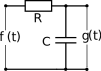
\includegraphics[scale=0.8]{Chapter_6/v6-RC.pdf}
\caption{\footnotesize Интегрирующая $RC$-цепочка}
\figmark{RC}
\end{wrapfigure}

\begin{exmpl}\label{exmpl:RC}
Найдём частотную характеристику $RC$-цепочки (рис.~\figref{RC}).
Повторяя рассуждения из Примера~\ref{exmpl:RLC} при $L=0$, получим
\[
\lambda(\omega) = \frac{1}{1+i\omega \tau_C},
\]
где $\tau_C=RC$ --- постоянная времени $RC$-цепочки.

При $\omega \gg 1/\tau_C$ имеем $\lambda \approx \frac{1}{i\omega\tau_C} \to 0$,
то есть $RC$-цепочка является простейшим \emph{фильтром высоких частот}.

В этом пределе можно выразить результат действия цепочки в явном виде.
При $\omega\tau_C\gg1$ напряжение на конденсаторе $q/C$ мал\'{о} по сравнению
с напряжением $\dot{q}R$ на резисторе, поэтому
\[
\dot{q} R \approx f(t) \qquad \to \qquad g(t) = \frac{q}{C} = \frac{1}{\tau_C}\int\limits_0^t f(t')\,dt'.
\]
Таким образом, фильтрация высокочастотных гармоник сводится к интегрированию
входного сигнала (подумайте, почему интеграл от быстропеременной функции
по достаточно большому интервалу оказывается мал).
\end{exmpl}

\section{Спектральное разложение}

Итак, при изучении линейных систем (фильтров) возникает необходимость
представления произвольного сигнала $f(t)$ в виде
\begin{equation}
    \eqmark{Fourier series}
    f(t)=\sum\limits_n c_n e^{i\omega_n t}.
\end{equation}
Представление \eqref{Fourier series} называется разложением сигнала~$f(t)$ в
\important{ряд Фурье}, а отдельные слагаемые ряда (составляющие
гармонические колебания) $c_n e^{i\omega_n t}$ называют \important{гармониками}.
Совокупность коэффициентов~$\{c_n\}$ называется \important{спектром} функции~$f(t)$.
Коэффициент~$c_n$ представим в виде $c_n=a_ne^{i\varphi_n}$, где
модуль $a_n=|c_n|$ определяет \emph{амплитуду} гармоники частоты~$\omega_n$,
а аргумент $\varphi_n=\arg c_n$~--- \emph{начальную фазу}.

В курсах математического анализа доказывается, что
разложение~\eqref{Fourier series} может быть осуществлено в общем случае (при
некоторых физически несущественных
ограничениях на~$f(t)$), причем \emph{единственным} образом.
То есть, существует единственный набор необходимых частот~$\omega_n$ и
единственный набор отвечающих этим частотам амплитуд~$a_n$ и фаз~$\varphi_n$,
обеспечивающих представление функции~$f(t)$ в виде суперпозиции гармонических
функций. Соответствующие формулы для этих коэффициентов мы получим ниже.

Отметим важное свойство гармонических функций.
Колебание $e^{i\omega_0 t}$ частоты~$\omega_0$ не может быть
представлено суперпозицией гармонических колебаний $\sum c_n e^{i\omega_n t}$
других частот $\omega_n\ne\omega_0$, какие бы коэффициенты~$c_n$, т.\,е.
амплитуды и фазы слагаемых гармоник, мы ни подбирали. В~математике это
свойство называют \important{ортогональностью}: функция $e^{i\omega_0 t}$
не имеет <<проекции>> на любую другую функцию $e^{i\omega_nt}$ при
$\omega_0\ne\omega_n$ (подобно тому как вектор, параллельный оси~$z$,
невозможно представить в виде суммы векторов, параллельных осям~$x$ и~$y$).

Для \emph{действительных} функций $f(t)$, которые как правило и представляют интерес,
наряду с разложением \eqref{Fourier series} часто используется разложение
в ряд Фурье вида%
\footnote{Также можно использовать эквивалентное разложение
\[f(t)=\sum\limits_{n=0}^{\infty} A_n \cos(\omega_n t) + B_n \sin(\omega_n t),\]
где $a_n=\sqrt{A_n^2+B_n^2}$, $\tg \varphi_n = \frac{B_n}{A_n}$.}
\begin{equation}
    \eqmark{Fourier-real-valued function}
    f(t)=\sum\limits_{n=0}^{\infty} a_n \cos(\omega_n t+\varphi_n ),
\end{equation}
где $a_n$, $\varphi_n$~--- действительные константы. Найдём связь между
коэффициентами разложений \eqref{Fourier series} и \eqref{Fourier-real-valued function}.
Пользуясь формулой Эйлера
\begin{equation}
    \eqmark{euler}
    \cos\alpha=\frac{e^{i\alpha}+e^{-i\alpha}}{2},
\end{equation}
представим каждое слагаемое \eqref{Fourier-real-valued function} в виде
\begin{equation*}
    a_n\cos(\omega_nt+\varphi_n)=\frac{a_n}{2}e^{i\varphi_n}\,e^{i\omega_n
t}+\frac{a_n}{2}e^{-i\varphi_n}\,e^{-i\omega_n t},
\end{equation*}
откуда ясно, что разложения \eqref{Fourier series} и
\eqref{Fourier-real-valued function} будут тождественны, если суммирование в
\eqref{Fourier series} проводить как по положительным частотам~$\omega_n$
(имеющим понятный физический смысл), так и по отрицательным (формально введённым)
частотам $\omega_{-n}=-\omega_n$, причём соответствующие коэффициенты имеют вид
\begin{equation}
    \eqmark{Fourier-coefficient}
    c_n =\frac{1}{2}a_n e^{i\varphi_n},
    \qquad c_{-n}=\frac{1}{2}a_n e^{-i\varphi_n}
\end{equation}
(коэффициенты $c_{-n}$ соответствуют отрицательным частотам~$-\omega_n)$,
т.\,е каждому слагаемому $a_n\cos(\omega_nt+\varphi_n)$ ряда \eqref{Fourier series}
соответствуют два слагаемых $c_ne^{i\omega_n t}$ и
$c_{-n}e^{-i\omega_n t}$ ряда \eqref{Fourier-real-valued function}.
% Нетрудно получить формулы обратного перехода от $\{c_n\}$ к
% $\{a_n,\varphi_n\}$:
% \begin{equation}
%      \eqmark{Fourier-coefficient-reverse}
%     a_n = 2|c_n|\qquad \varphi_n = \arg c_n.
% \end{equation}

\begin{figure}[ht]
%     \psfragfig[width=0.7\textwidth]{Images/Chapter_6/7}{%
%     \psfrag{a}[ct]{$\omega_1$}
%     \psfrag{b}[ct]{$\omega_2$}
%     \psfrag{c}[ct]{$\omega_3$}
%     \psfrag{d}[ct]{$\omega_4$}
%     \psfrag{e}[ct]{$-\omega_{1}$}
%     \psfrag{f}[ct]{$-\omega_{2}$}
%     \psfrag{g}[ct]{$-\omega_{3}$}
%     \psfrag{h}[ct]{$-\omega_{4}$}
%     \psfrag{o}[ct]{0}
%     \psfrag{1}[cb]{$\varphi_1$}
%     \psfrag{2}[cb]{$\varphi_2$}
%     \psfrag{3}[cb]{$\varphi_3$}
%     \psfrag{4}[cb]{$\varphi_4$}
%     \psfrag{x}{$\omega$}
%     \psfrag{y}{$\{c_n\}$}
%     \psfrag{z}{$\{a_n\}$}
%     \psfrag{A}{а)}
%     \psfrag{B}{б)}}
\centering\includegraphics[width=0.6\textwidth]{Chapter_6/7}
    \caption{Спектр в комплексном и действительном представлениях}
    \figmark{spectrum}
\end{figure}

Мы видим, что при разложении \emph{действительных} функций~$f(t)$ в ряд Фурье
коэффициенты разложения~$c_{-n}$ на отрицательных
частотах связаны с коэффициентами~$c_n$ простым соотношением
\[
c_{-n}=c_{n}^*,
\]
где звёздочка обозначает \emph{комплексное сопряжение}.
Таким образом, гармоники с отрицательными частотами не несут какой-либо
дополнительной информации о действительном сигнале~$f(t)$.

Спектр функции~$f(t)$ принято изображать в виде графика
(рис.~\figref{spectrum}): длина стрелочки на каждой частоте~$\omega_n$
определяется модулем коэффициента~$c_n$ (т.~е. амплитудой соответствующего
гармонического колебания). Следует указать также начальные фазы~$\varphi_n$
спектральных компонент.

Соответствующее разложение \eqref{Fourier-real-valued function} (в ряд
косинусов) представлено на графике рис. \figref{spectrum}б: здесь нет
отрицательных частот, а длины стрелочек на положительных частотах в соответствии с
\eqref{Fourier-coefficient} удваиваются. При этом постоянные составляющие
(на частоте $\omega=0$) в разложениях \eqref{Fourier series} и
\eqref{Fourier-real-valued function} одинаковы: $a_0=c_0$.

\subsection{Спектр периодического процесса}
Получим коэффициенты разложения в ряд Фурье для периодического колебательного
процесса общего вида $f(t)=f(t+T)$, где $T$~--- период процесса.
Покажем, что в этом случае функция~$f(t)$ может быть представлена
бесконечной суммой гармонических колебаний с кратными частотами~$\omega_n=n\omega_0$,
где $\omega_0=2\pi/T$, $n$~--- целое число:
\begin{equation}
    \eqmark{Fourier-periodic osc}
    f(t)=\sum_{n=-\infty}^{\infty} c_n e^{in\omega_0 t}.
\end{equation}
Нетрудно видеть, что все слагаемые в \eqref{Fourier-periodic osc}~---
периодические функция с периодом, кратным $T$, и они полностью исчерпывают
набор гармонических функций, удовлетворяющих условию $f(t)=f(t+T)$.
Таким образом, периодическая функция имеет \important{дискретный}
спектр с кратными частотами.

Спектр --- то есть набор коэффициентов~$\{c_n\}$ ---
можно найти следующим образом: домножим обе части равенства
\eqref{Fourier-periodic osc} на $e^{-im\omega_0 t}$ и
проинтегрируем по времени~$t$ за период (например от~$0$ до~$T$). Получим
\begin{equation*}
    \int\limits_{0}^{T} f(t)e^{-im\omega_0t}\,dt=\sum_n c_n\int\limits_{0}^{T}
e^{i(n-m)\omega_0 t}\,dt.
\end{equation*}
Вычислим интеграл в правой части:
\begin{equation*}
    \int\limits_{0}^{T}e^{i(n-m)\omega_0 t}dt =
%     = \left.\frac{e^{i(n-m)\omega_0 t}}{i(n-m)\omega_0} \right|_0^{T}
    \begin{cases}
        0 & \text{при~}n\ne m,\\
        T & \text{при~}n = m.
    \end{cases}
\end{equation*}
% (время $T$ есть целое число периодов колебания функций
% $\cos(n-m)\omega_0t$ и $\sin(n-m)\omega_0t$, поэтому интегралы от них
% на отрезке $[0,\,T]$ зануляются).
Таким образом, находим
\begin{equation}
    \eqmark{coef-Fourier-periodic osc}
    c_n=\frac{1}{T}\int\limits_{0}^{T} f(t)e^{-in\omega_0 t}\,dt.
\end{equation}
Это и есть искомое правило нахождения коэффициентов разложения периодической
функции в гармонический ряд Фурье.

\begin{wrapfigure}[10]{o}{0.5\textwidth}
%     \psfragfig[width=0.5\textwidth]{Images/Chapter_6/12}{%
%     \psfrag{x}{$t$}
%     \psfrag{1}[rb]{1}
%     \psfrag{f}{$f(t)$}
%     \psfrag{a}[cb]{$\tau$}
%     \psfrag{b}[cb]{$T$}}
\centering\includegraphics[width=0.5\textwidth]{Chapter_6/12}
    \caption{\footnotesizeПериодическая последовательность импульсов}
    \figmark{meander}
\end{wrapfigure}

\begin{exmpl}\label{exmpl:square-zug}
Найдём спектр периодической последовательности прямоугольных
импульсов длительности~$\tau$ с периодом следования импульсов $T>\tau$
(рис.~\figref{meander}, начало отсчёта выбрано так, что~$f(t)$ --- чётная
функция).

Используя \eqref{coef-Fourier-periodic osc} на интервале интегрирования
$-T/2\le t \le T/2$, с учётом того, что функция~$f(t)$ отлична от нуля и
равна единице лишь в области $|t|<\tau/2$, находим
\begin{equation}
    \eqmark{impulses-spectrum}
    c_n =\frac{1}{T}\int\limits_{-\tau/2}^{\tau/2} e^{-in\omega_0 t}\,dt
    =\frac{\tau}{T}\cdot \frac{\sin \left(n\omega_0\tau/2\right)}{n\omega_0\tau/2} =
     \frac{\sin \left(\pi n \tau/T\right)}{\pi n}.
\end{equation}

\begin{figure}[h!]
%     \psfragfig[width=\textwidth]{Images/Chapter_6/13}{%
%     \psfrag{x}{$\omega$}
%     \psfrag{y}{$c_n$}
%     \psfrag{0}[tr]{0}
%     \psfrag{1}[ct]{$\vphantom{2}\omega_0$}
%     \psfrag{2}[ct]{$2\omega_0$}
%     \psfrag{c}{$C(\omega)$}
%     \psfrag{d}[ct]{$2\Delta\omega$}}
\centering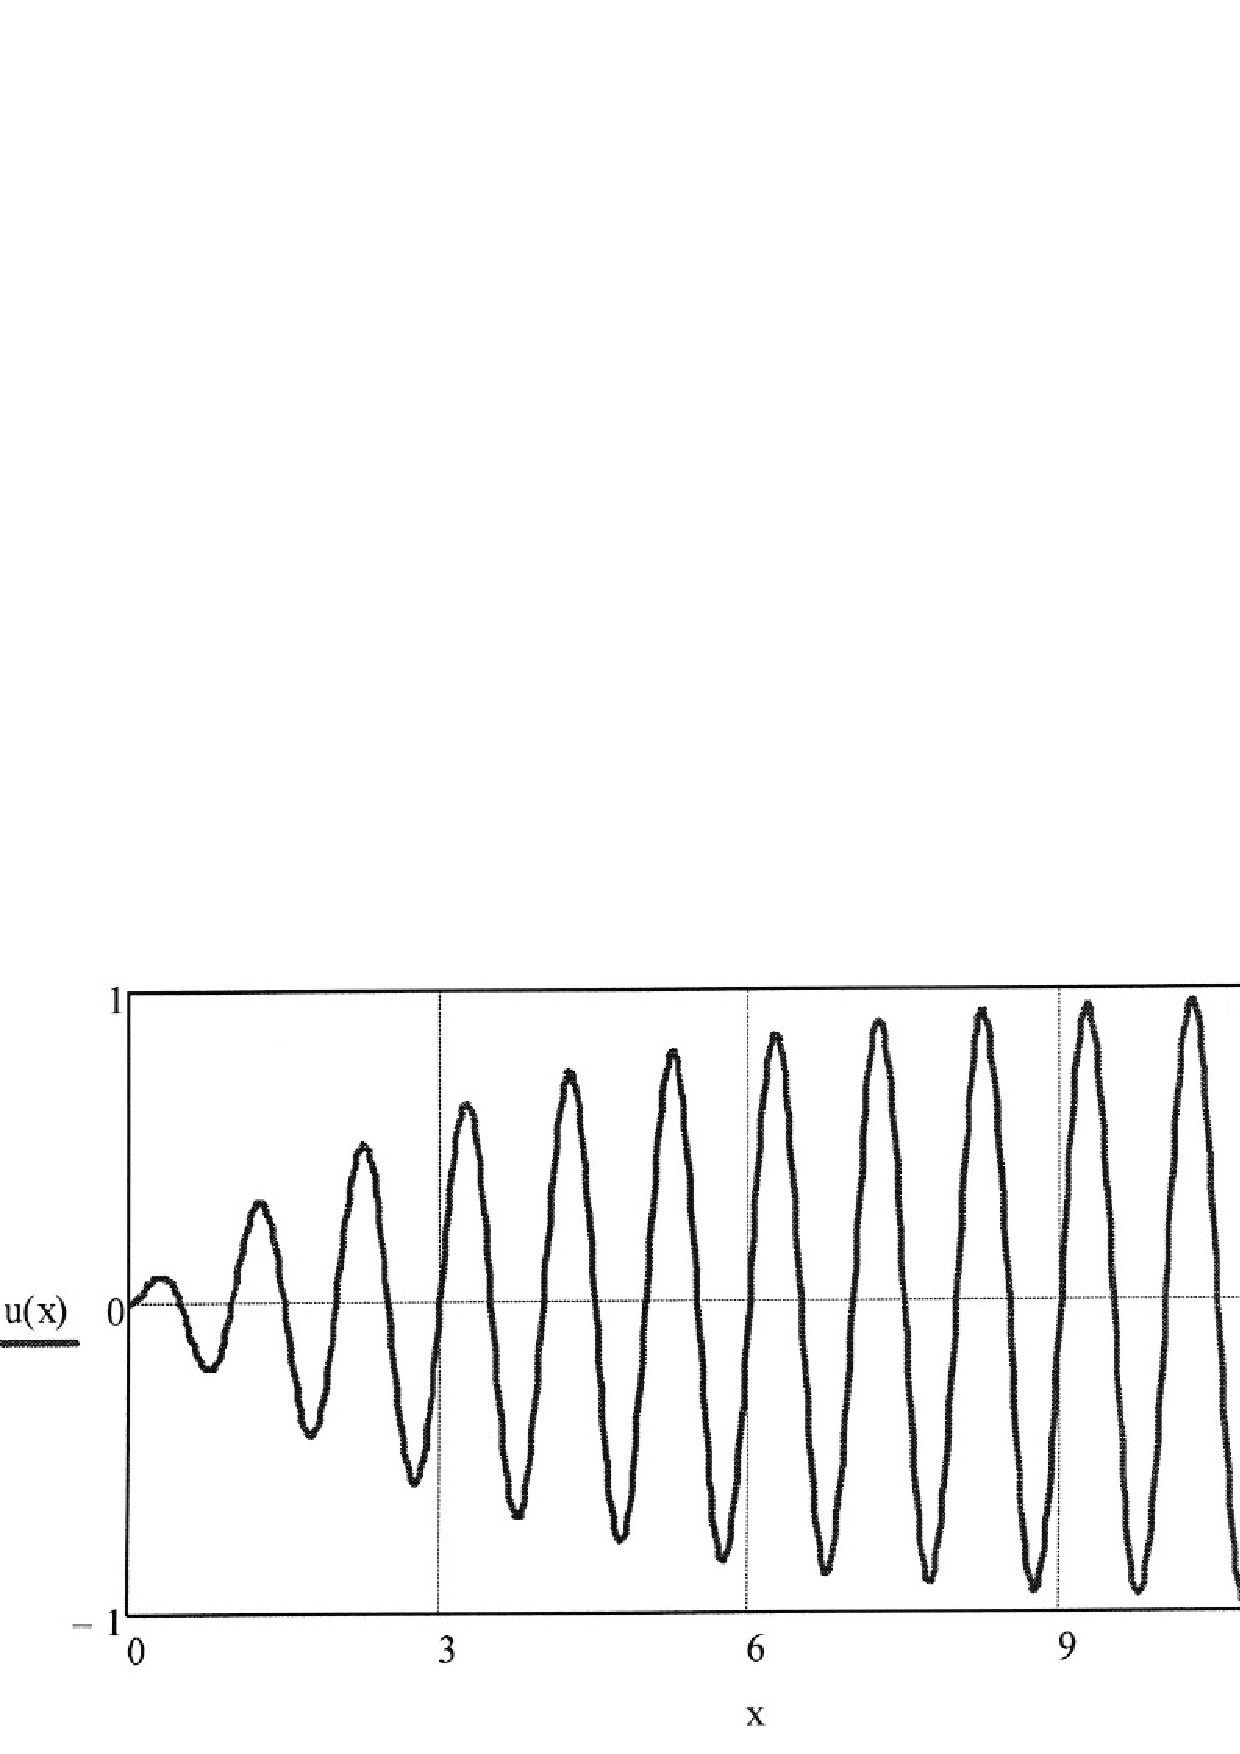
\includegraphics[width=0.9\textwidth]{Chapter_6/13.pdf}
    \caption{Спектр периодической последовательности импульсов
        (рисунок приведён для случая $\tau=\frac13 T$)}
    \figmark{spectrum-meander}
\end{figure}

Спектр $\{c_n\}$ показан на рис.~\figref{spectrum-meander}.
Пунктирной кривой изображена огибающая функция
\begin{equation*}
    C(\omega) =\frac{\tau}{T}\cdot \frac{\sin\omega\tau/2}{\omega\tau/2}.
\end{equation*}
При $\omega=n\omega_0$ эта функция принимает значение $C(n\omega_0)=c_n$.
Полуширина $\Delta \omega$ главного максимума этой функции определяется
условием $\sin\omega\tau/2=0$:
\begin{equation*}
    \Delta\omega \cdot \frac{\tau}{2}=\pi\qquad \text{или} \qquad \Delta \omega
\cdot \tau =2\pi.
\end{equation*}
Как видно из рисунка, спектральные гармоники,
имеющие заметную амплитуду, сосредоточены в интервале частот
$|\omega|\lesssim\Delta\omega=2\pi/\tau$.
\end{exmpl}


\subsection{Спектр непериодического процесса}

Рассмотрим задачу разложения в спектр произвольного непериодического
сигнала $f(t)$.

Ответ можно получить, воспользовавшись результатом
\eqref{coef-Fourier-periodic osc} для разложения периодической функции
и устремляя период к бесконечности $T\to \infty$.

\begin{wrapfigure}[9]{o}{0.5\textwidth}
    \centering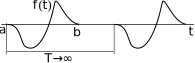
\includegraphics[width=\linewidth]{Chapter_6/v6-finf.pdf}
    \caption{Непериодический процесс как предел периодического}
    \figmark{finf}
\end{wrapfigure}

Пусть функция $f(t)$ отлична от нуля на некотором конечном интервале
$t\in[a,\,b]$, а вне его обращается в ноль. Рассмотрим периодическую функцию
с достаточно большим периодом повторения $T>b-a$, составленную из <<кусков>>
функции $f(t)$. Посмотрим, что происходит со спектральным разложением
такой функции по мере увеличения $T$.

Видно, что частоты $\omega = n \frac{2\pi}{T}$ гармоник, по которым идёт
разложение, будут в пределе $T\to \infty$ располагаться всё плотнее друг к другу.
Интервал между соседними частотами равен $\Delta \omega = \frac{2\pi}{T}$.
Таким образом, имеем $\Delta \omega\to 0$ и, следовательно,
спектр должен стать \important{непрерывным}.

Тогда спектральное разложение превратится из суммы в интеграл:
\[
 f(t) = \frac{1}{\Delta \omega}\sum c_n e^{i\omega_n t} \Delta \omega \to
 \frac{T}{2\pi} \int\limits_{-\infty}^{\infty} c_n e^{i\omega_n t} d\omega,
\]
Обозначая $C(\omega)=c_n T$, запишем искомое разложение как
\begin{equation}
\eqmark{Fourier integral}
f(t) = \frac{1}{2\pi} \int\limits_{-\infty}^{\infty} C(\omega) e^{i\omega t} d\omega,
\end{equation}
где $C(\omega)$ найдём из \eqref{coef-Fourier-periodic osc}:
\begin{equation}
\eqmark{Fourier integral-coef}
 C(\omega) =
%  \frac{c_n}{\Delta \omega} =
%  \frac{1}{\Delta \omega T}\int\limits_{-\infty}^{\infty}
%  f(t) e^{-i\omega t} dt \to
\int\limits_{-\infty}^{\infty} f(t) e^{-i\omega t} dt.
\end{equation}

Множитель $C(\omega)=a(\omega)e^{i\varphi(\omega)}$ показывает, с каким
<<весом>> (т.~е. с какой амплитудой $a(\omega)$ и с какой начальной фазой
$\varphi(\omega)$) необходимо складывать гармонические
колебания разных частот, чтобы при суммировании (интегрировании) образовать
заданный сигнал $f(t)$. Функция $C(\omega)$ называется \important{спектром}
или \important{преобразованием Фурье} сигнала~$f(t)$.
Видно, что в общем случае необходим непрерывный набор (\emph{континуум}) гармоник.

Соотношение \eqref{Fourier integral-coef} также называют
\important{прямым преобразованием Фурье}, а формулу \eqref{Fourier integral}~---
\important{обратным преобразованием Фурье}.
Связь функцией и её спектром символически можно записать как
\[
C(\omega) = \hat{\mathcal{F}}[f(t)],\qquad f(t) = \hat{\mathcal{F}}^{-1}[C(\omega)],
\]
где $\hat{\mathcal{F}}$ и~$\hat{\mathcal{F}}^{-1}$~--- условное обозначение
для прямого и обратного преобразования Фурье (заметим, что
эти преобразования \emph{линейны}).

\begin{exmpl}\label{exmpl:square}
Найдём спектр прямоугольного импульса длительности $\tau$
единичной амплитуды (рис.~\figref{spectrum-one meander}а). Используя
\eqref{Fourier integral-coef}, получаем
\begin{equation}
    \eqmark{spectrum-impulse}
    C(\omega)=\int\limits_{-\tau/2}^{\tau/2} e^{-i\omega
t}\,dt=\frac{1}{-i\omega}\int\limits_{-\tau/2}^{\tau/2} e^{-i\omega t}\,
d(-i\omega t)=\tau\frac{\sin\omega\tau/2}{\omega\tau/2}.
\end{equation}
Функция $C(\omega)$ показана на рис.~\figref{spectrum-one meander}б.
\begin{figure}[h!]
   \centering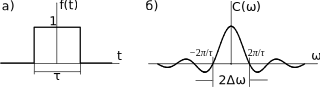
\includegraphics{Chapter_6/v6-single.pdf}
    \caption{Одиночный импульс (а) и его спектр (б)}
    \figmark{spectrum-one meander}
\end{figure}

Полезно сравнить спектр отдельного импульса со спектром периодической
последовательности одинаковых импульсов (рис.~\figref{spectrum-meander}).
Вместо \emph{дискретного} спектра $\{c_n\}$ мы получили
\emph{непрерывный} спектр~$C(\omega)$, причём
спектр импульса $C(\omega)$ (с множителем $1/T$) представляет собой
<<огибающую>> частокола спектральных компонент $c_n$
периодической последовательности импульсов.

Заметим также, что, как видно из графика, основной вклад дают гармоники, частоты
которых заполняют интервал $|\Delta\omega|<2\pi/\tau$. Это~--- полуширина
главного максимума функции $\frac{\sin\omega\tau/2}{\omega\tau/2}$. Диапазон
частот $\Delta\omega$ можно назвать характерной \emph{шириной спектра}
$C(\omega)$.
\end{exmpl}


\subsection{Соотношение неопределённостей}

При рассмотрении Примеров~\ref{exmpl:square-zug} и~\ref{exmpl:square},
мы получили замечательное соотношение, связывающее между собой
длительность~$\Delta t$ сигнала с шириной его спектра~$\Delta \omega$:
\begin{equation}
    \eqmark{indeterminacy relation}
    \Delta t \cdot \Delta\omega \sim 2\pi.
\end{equation}

Оказывается, это соотношение имеет универсальный характер.
Оно остаётся справедливым по порядку величины для произвольного сигнала $f(t)$.
% (соответствующую строгую теорему можно найти в курсах математического анализа).
Чем больше длительность сигнала~$\Delta t$ (либо больше интервал времени,
в течение которого происходит его заметное изменение), тем \'{у}же спектр
сигнала~$\Delta\omega$, и, наоборот, чем короче сигнал (или быстрее происходит
изменение сигнала), тем шире его спектр, т.\,е. требуется более широкий интервал
частот гармонических колебаний, образующих в сумме данный сигнал.
В этом состоит смысл формулы \eqref{indeterminacy relation},
которая называется \important{соотношением неопределённостей}.

В общем случае, если у сигнала есть какое-то характерное время~$\Delta t$,
в его спектре обязательно возникнет некоторый характерный масштаб
$\Delta \omega \sim 2\pi /\Delta t$. Например, рассмотрим ограниченную
последовательность периодических импульсов с полной длительностью~$t_0$,
периодом~$T\ll t_0$ и длительностью каждого импульса~$\tau\ll T$.
Сигнал и его спектр представлены на рис.~\figref{indeterm}
(он может быть без труда рассчитан из формулы \eqref{Fourier integral-coef}
с использованием результатов разобранных выше Примеров~\ref{exmpl:RLC}
и~\ref{exmpl:square-zug}). На спектре видно три характерных масштаба частоты:
наибольший масштаб~$\Delta \omega_{\tau} = 2\pi/\tau$ задаёт ширину всего спектра,
масштаб~$\Delta \omega_T = 2\pi / T$ есть расстояние между соседними
спектральными пиками, и наконец наименьший машстаб $\Delta \omega_0 = 2\pi /t_0$,
соответствующий наибольшему характерному времени~$t_0$,
определяет ширину каждого пика.

\begin{figure}[h!]
\centering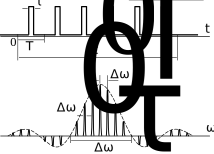
\includegraphics[scale=1.0]{Chapter_6/v6-indeterm.pdf}
\caption{Связь ширины спектра с характерными временными масштабами}
\figmark{indeterm}
\end{figure}

\subsection{Спектральный метод в задаче линейной фильтрации}

Сформулируем ещё раз алгоритм решения задачи линейной фильтрации
спектральным методом (методом Фурье) с учётом полученных соотношений.

Для нахождения отклика линейной системы $g(t)$ на воздействие $f(t)$
нужно:
\begin{enumerate}
    \item представить входной сигнал $f(t)$ в виде ряда
    \eqref{Fourier series} или интеграла Фурье \eqref{Fourier integral},
где спектр $\hat{\mathcal{F}}[f]$ (функция $C(\omega)$ или набор $\{c_n\}$)
находится с помощью соотношений \eqref{coef-Fourier-periodic osc}
или~\eqref{Fourier integral-coef};

    \item найти частотную характеристику фильтра
$\lambda(\omega)$, т.\,е. функцию отклика фильтра на гармоническое внешнее воздействие
единичной амплитуды:
\begin{equation*}
    e^{i\omega t}\to\fbox{$\hat\Lambda$}\to \lambda(\omega)e^{i\omega t};
\end{equation*}

    \item просуммировать отклики на каждое гармоническое
    слагаемое входного сигнала, что даёт спектр выходного сигнала:
    \begin{equation*}
    \sum c_n e^{i\omega_n t} \to\fbox{$\hat\Lambda$}\to \sum \lambda(\omega_n)c_n e^{i\omega_n t},
    \end{equation*}
    или
    \begin{equation*}
    \int C(\omega) e^{i\omega t} \to\fbox{$\hat\Lambda$}\to
    \int \lambda(\omega)\cdot C(\omega)e^{i\omega t};
    \end{equation*}
    \item восстановить выходной сигнал $g(t)$ по его спектру
    (обратное преобразование Фурье).
\end{enumerate}
Всю схему можно записать кратко одной формулой:
    \begin{equation}
        \eqmark{linear-filter-fourier}
    g(t) = \hat{\mathcal{F}}^{-1}\!
    \left[\lambda(\omega)\cdot \hat{\mathcal{F}}[f(t)]\right].
    \end{equation}


\begin{wrapfigure}[14]{o}{0.25\textwidth}
     \centering\includegraphics{Chapter_6/v6-delta.pdf}
     \caption{\footnotesize Предельный переход к дельта-импульсу}
\end{wrapfigure}

\begin{exmpl}\label{exmpl:delta}
Устремим длительность импульса из предыдущего примера к нулю $\tau\to 0$,
при этом его амплитуду $A$ будем наращивать так, чтобы площадь
под его графиком была постоянной (единичной): $\int f(t) = A \tau = 1$.
Такой импульс физике обозначают как $\delta(t)$ и называют \emph{дельта-импульсом}
(или \emph{дельта-функцией}).

Поскольку $\sin x/x\to 1$ при $x\to 0$,
предельный переход \eqref{spectrum-impulse} даёт простой результат:
\begin{equation}
    \eqmark{spectrum-impulse}
    C(\omega)\to A\tau =1.
\end{equation}
То есть спектр бесконечно узкого импульса единичной площади (дельта-функции)
есть единичная константа. Заметим, что и здесь выполняется соотношение
неопределённостей: бесконечно узкий импульс даёт бесконечно широкий спектр.

Этот результат позволяет придать новый смысл частотной характеристике
(функции отклика) $\lambda(\omega)$ некоторого фильтра.
Если спектр входного сигнала $f(t)$ есть единичная константа,
то как следует из соотношения \eqref{linear-filter-fourier},
откликом системы будет функция $g(t)$, спектр которой совпадает
с $\lambda(\omega)$. Таким образом, \emph{обратное преобразование Фурье
от функции отклика системы есть её реакция на единичный дельта-имульс}.
\end{exmpl}


\subsection{Физический смысл спектрального разложения}

Разложение функции $f(t)$ в ряд или интеграл Фурье может показаться
абстрактной математической операцией --- некоторым трюком, не имеющим
под собой физического содержания. Попробуем ответить на вопрос,
можно ли \emph{измерить} амплитуды спектральных компонент $f(t)$,
тем самым приписав им прозрачный физический смысл.

Рассмотрим колебательный $RLC$-контур и подадим на его вход некоторый сигнал $f(t)$.
Для простоты ограничимся периодической функцией.

Пусть собственная частота контура равна $\Omega$, а добротность его
достаточно велика: $Q=\Omega/2\gamma \gg 1$ ($\gamma$ --- коэффициент затухания).

Пусть известно спектральное разложение $f(t)=\sum c_n e^{i\omega_n t}$.
После <<фильтрации>> через контур на выходе получим сигнал со
спектральными компонентами $g(t)=\sum g_n e^{i\omega_n t}$,
где $g_n = \lambda(\omega_n) c_n$ для каждого $n$,
$\lambda(\omega)$ --- частотная характеристика $RLC$-контура, найденная
выше (см. Пример~\ref{exmpl:RLC}). Нетрудно видеть, что такое преобразование резко
(примерно в $Q$ раз) усиливает частоты входного сигнала, близкие к
$\Omega$ (т.\,е. к \emph{резонансу}), и ослабляет далёкие.
В~пределе идеального контура ($Q\to \infty$), в спектре сигнала на выходе
останется единственная~--- резонансная~--- частота.
Сигнал $g(t)$ будет гармоническим колебанием с частотой $\Omega$:
$g(t) \propto c(\Omega) e^{i\Omega t}$,
причём его амплитуда будет пропорциональна амплитуде гармоники с этой
частотой в разложении исходной функции $f(t)$ (а если в этом разложении не было
гармоники $\omega_n=\Omega$, результирующая амплитуда будет нулевой).

Мы видим, что высокодобротный колебательный контур <<отфильтровывает>> из подаваемого
на него сигнала те спектральные компоненты, частоты которых близки к
его собственной $\Omega$. По амплитуде отклика можно измерить и амплитуду
гармоники в исходном сигнале. Меняя собственную частоту контура $\Omega$
(например, изменяя ёмкость конденсатора), можно в принципе просканировать весь
диапазон частот, измерив таким образом амплитуды всех спектральных
компонент~$c_n$ в разложении $f(t)=\sum c_n e^{i\omega_n t}$. Итак,
спектр сигнала может быть измерен непосредственно и описанная схема измерения
позволяет придать спектральному разложению наглядный физический смысл.

\begin{exmpl}\label{exmpl:zug-RLC}
Рассмотрим колебательный $RLC$-контур с собственной
частотой~$\Omega$ и добротностью $Q\gg 1$, в котором мы попытаемся раскачать колебания,
подавая на вход периодическую последовательность коротких импульсов
с периодом $T$ и длительностью $\tau$. Можно ли раскачать колебания в контуре
до сколь-нибудь значимых амплитуд, если частота повторения импульсов
$\omega_0=2\pi/T$ много меньше резонасной частоты контура $\Omega$,
$\omega_0\ll \Omega$?

\begin{figure}[h!]
 \centering\includegraphics[width=\textwidth]{Chapter_6/v6-impulse-filter.pdf}
 \caption{\footnotesize Изменение спектра периодической последовательности импульсов (слева)
 в результате фильтрации колебательным контуром (справа) при резонансе с одной
 из высокочастотных гармоник. Расчёт проведён
 для $Q=50$, $\omega_0=\Omega/7$, $\tau=T/4$}
 \figmark{impulse-filter}
\end{figure}

Для нахождения амплитуды результирующих колебаний нужно перемножить
спектр периодической последовательности $\{c_n\}$
(см. Пример~\ref{exmpl:square-zug}, \eqref{impulses-spectrum})
и частотную характеристику колебательного контура $\lambda(\omega)$
(см. Пример~\ref{exmpl:RLC}, \eqref{RLC-lambda}).
Возможный результат такого преобразования представлен на рис.~\figref{impulse-filter}.
Видно, что благодаря существованию в спектре входного сигнала высокочастотных
гармоник $\omega_n = n \omega_0$, при выполнении условия
$\Omega = n \omega_0$, где $n$ --- целое, и при достаточно высокой добротности,
такая раскачка колебаний возможна.

Из \eqref{impulses-spectrum} видно, что амплитуды гармоник $|c_n|$ убывают
с ростом $n$ как $1/n$. С другой стороны, из \eqref{RLC-lambda} можно получить,
что в резонансе сигнал усиливается в $Q$ раз.
Таким образом, раскачать колебания в высокодобротном $RLC$-контуре можно
с помощью периодических импульсов, частота повторения $\omega_0=2\pi/T$
которых может быть существенно меньше резонансной,
вплоть до $\omega_0 \sim \Omega / Q \ll \Omega $.
\end{exmpl}

\subsection[Свойства преобразования Фурье]{%
    Свойства преобразования Фурье}
% \protect\footnote{При первом чтении данный раздел можно пропустить.}}

Рассмотрим некоторые свойства спектрального разложения (преобразования Фурье),
которые могут быть полезны при расчёте спектров.

\begin{wrapfigure}{o}{0.3\textwidth}
 \centering\includegraphics{Chapter_6/v6-modul.pdf}
 \caption{}
 \figmark{modul}
\end{wrapfigure}

\paragraph{Спектр огибающей, заполненной высокочастотным сигналом.}
Пусть $C_0(\omega)$ --- спектр некоторой функции $f_0(t)$.
Найдём спектр $C(\omega)$ функции
\[
f(t)=f_0(t)\cos(\omega_0 t).
\]
Здесь $f_0(t)$ имеет смысл <<огибающей>>, заполненной колебаниями
с частотой~$\omega_0$ (см. рис.~\figref{modul}).

Используя формулу Эйлера \eqref{euler}, запишем
\begin{equation*}
    f(t)=\frac{1}{2}f_0(t)e^{i\omega_0t}+\frac{1}{2}f_0(t)e^{-i\omega_0t}.
\end{equation*}
Пользуясь \eqref{Fourier integral-coef}, найдём спектр
функции $f_0(t)e^{i\omega t}$:
\begin{equation}
    \eqmark{task-spectrum-shift}
    \int\limits_{-\infty}^\infty f_0(t)e^{i\omega_0 t}\cdot e^{-i\omega
t}\,dt=\int\limits_{-\infty}^\infty
f_0(t)e^{-i(\omega-\omega_0)t}\,dt=C_0(\omega-\omega_0),
\end{equation}
т.~е. при умножении на $e^{i\omega_0 t}$ исходный спектр
\emph{сдвигается} по оси частот на величину $\omega_0$
(рис.~\figref{task-shift-spectrum}).

\begin{figure}[h!]
\centering\includegraphics{Chapter_6/v6-shift.pdf}
\caption{Смещение спектра при домножении сигнала на $e^{i\omega_0 t}$}
\figmark{task-shift-spectrum}
\end{figure}

%\begin{equation}
%   \eqmark{task-freq-shift}
%   C(\omega)=e^{-i\omega\tau}\int_{-\infty}^\infty f_0(t')e^{-i\omega
% t'}\,dt'=C_0(\omega)\cdot e^{-i\omega\tau},
%\end{equation}
%или символически $f_0(t-\tau) \leftrightarrow C_0(\omega)e^{-i\omega\tau}$,
% т.е. смещение сигнала во времени на $\tau$ (запаздывание) приводит к умножению
% его спектра на $e^{-i\omega\tau}$ (теорема смещения).
%

Отсюда находим искомый спектр:
\begin{equation}
    \eqmark{task-2shift-spectrum-cos}
    C(\omega)=\frac{1}{2}C_0(\omega-\omega_0)+\frac{1}{2}C_0(\omega+\omega_0).
\end{equation}
Если частота $\omega_0$ существенно превосходит характерную ширину $\Delta \omega$
спектра огибающей, $\omega_0 \gg \Delta \omega$, то слагаемые
\eqref{task-2shift-spectrum-cos} не накладываются друг на друга.
Тогда искомый спектр $C(\omega)$ получается из $C_0(\omega)$
простым смещением по оси частот влево и вправо на <<несущую>>
частоту $\omega_0$ (с домножением на 1/2, см. рис.~\figref{task-2shift-spectrum-cos}).

\begin{figure}[h!]
%     \psfragfig[width=0.8\textwidth]{Images/Chapter_6/15b}{%
%     \psfrag{x}{$\omega$}
%     \psfrag{y}{$C_0(\omega)$}
%     \psfrag{z}{$C(\omega)$}
%     \psfrag{a}[ct]{$-\omega_0$}
%     \psfrag{b}[ct]{$\omega_0$}}
\centering\includegraphics[width=0.8\textwidth]{Chapter_6/15b.pdf}
    \caption{Преобразование спектра при домножении на $\cos \omega_0 t$}
    \figmark{task-2shift-spectrum-cos}
\end{figure}

\begin{wrapfigure}{o}{0.5\textwidth}
%     \psfragfig[width=0.5\textwidth]{Images/Chapter_6/16}{%
%     \psfrag{t}{$t$}
%     \psfrag{f}{$f_0(t)$}
%     \psfrag{F}{$f(t)$}
%     \psfrag{a}[ct]{$\llap{$-$}\frac{\tau}{2}$}
%     \psfrag{b}[ct]{$\frac{\tau}{2}$}
%     \psfrag{A}{а)}
%     \psfrag{B}{б)}}
\includegraphics[width=0.5\textwidth]{Chapter_6/16}
    \caption{\footnotesize Прямоугольный импульс (а), ограничивающий синусоиду (б)}
    \figmark{one-zug}
\end{wrapfigure}

\begin{exmpl}\label{exmpl:one-zug}
Найдём спектр обрывка синусоиды с частотой $\omega_0$
длительностью $\tau$ (такой сигнал называют \important{цугом}).
Сигнал может быть представлен как
\[f(t)=f_0(t)\cos(\omega_0 t),\] где $f_0(t)$ --- единичный прямоугольный
импульс длительностью $\tau$ (см. рис.~\figref{one-zug}).

Пользуясь полученными ранее формулами для спектра прямоугольного импульса
\eqref{spectrum-impulse} и для смещения спектра \eqref{task-2shift-spectrum-cos},
получим
\begin{equation*}
C(\omega)=\frac{\tau}{2}\left[\frac{\sin(\omega-\omega_0)\tau/2}{
(\omega-\omega_0)\tau/2}+
\frac{\sin(\omega+\omega_0)\tau/2}{(\omega+\omega_0)\tau/2}
\right].
\end{equation*}
Спектры $C_0(\omega)$ и $C(\omega)$ представлены на
рис.~\figref{task-meander-train-spectrum}.

\begin{figure}[h!]
%     \psfragfig[width=0.8\textwidth]{Images/Chapter_6/17}{%
%     \psfrag{p}[br]{$\tau$}
%     \psfrag{q}{$\tau/2$}
%     \psfrag{w}{$\omega$}
%     \psfrag{f}{$C_0(\omega)$}
%     \psfrag{F}{$C(\omega)$}
%     \psfrag{a}[ct]{$\llap{$-$}\omega_0$}
%     \psfrag{b}[ct]{$\omega_0$}
%     \psfrag{A}{а)}
%     \psfrag{B}{б)}}
\centering\includegraphics[width=0.8\textwidth]{Chapter_6/17}
    \caption{Спектры а) прямоугольного импульса, б) импульса,
        заполненного синусоидой (цуга)}
    \figmark{task-meander-train-spectrum}
\end{figure}

\begin{figure}[h!]
\hfil
    \pic{0.5\textwidth}{Chapter_6/v6-zug}
    \caption{Периодическая последовательность цугов}
    \figmark{zug-zug}
\end{figure}

\paragraph{Упражнение.} Предлагаем читателю самостоятельно получить
спектр периодической последовательности цугов (см. рис.~\figref{zug-zug}).
\end{exmpl}


\begin{exmpl}\label{exmpl:exp}
Найдём спектр затухающих колебаний
\[
f(t) = e^{-\gamma t} \sin \omega_0 t\qquad (\text{при~}t\ge 0).
\]
По формуле \eqref{Fourier integral-coef} находим спектр затухающей
экспоненты (начинающейся с $t=0$):
\[
\hat{\mathcal{F}}[e^{-\gamma t}] =
\int\limits_0^{\infty} e^{-\gamma t - i\omega} dt =
\frac{1}{\gamma + i\omega}
\]
(ср. с Примером~\ref{exmpl:RC}).
Пользуясь формулой Эйлера для синуса
\[
\sin \alpha = \frac{e^{i\alpha} - e^{-i\alpha}}{2i},
\]
получим искомый спектр по формуле смещения \eqref{task-spectrum-shift}:
\[
C(\omega) = \frac{1}{2i} \left[\frac{1}{\gamma + i(\omega-\omega_0)} -
\frac{1}{\gamma + i(\omega+\omega_0)}\right] =
\frac{\omega_0}{\omega_0^2 + \gamma^2 - \omega^2 +2i\gamma \omega }.
\]

Обратим внимание, что если положить $\omega_0^2 =\Omega^2 - \gamma^2$,
полученный ответ совпадает (с точностью до константы)
с частотной характеристикой колебательного контура \eqref{RLC-lambda}.
Это не удивительно, поскольку именно затухающие колебания
$f(t) = e^{-\gamma t} \sin \omega_0 t$
возникают в колебательном контуре, если сообщить ему единичный дельта-импульс
(см. также Пример~\ref{exmpl:delta}).
\end{exmpl}

\paragraph{Теорема смещения.}
Найдём спектр $C(\omega)$ сигнала, смещённого по времени: $f(t)=f_0(t-\tau)$,
где $f_0(t)$ --- функция с известным спектром~$C_0(\omega)=\hat{\mathcal{F}}[f_0]$.

По определению имеем
\begin{equation*}
  C(\omega)=\hat{\mathcal{F}}[f(t)]=\int\limits_{-\infty}^\infty f_0(t-\tau)e^{-i\omega t}\,dt.
\end{equation*}
После замены переменных $t'=t-\tau$ ($dt=dt'$) получаем
\begin{equation*}
  C(\omega)=\int\limits_{-\infty}^\infty f_0(t') e^{-i\omega(t'+\tau)}\,dt'.
\end{equation*}
Множитель $e^{-i\omega\tau}$ (не зависящий от переменной интегрирования $t'$)
выносится из-под знака интеграла:
\begin{equation}
  \eqmark{task-freq-shift}
  C(\omega)=e^{-i\omega\tau}\int\limits_{-\infty}^\infty f_0(t')e^{-i\omega
t'}\,dt'= e^{-i\omega\tau} \cdot C_0(\omega),
\end{equation}
или символически
\[
\hat{\mathcal{F}}[f_0(t-\tau)] = e^{-i\omega\tau} \hat{\mathcal{F}}[f_0(t)],
\]
т.\,е. смещение сигнала во времени на $\tau$ (запаздывание)
приводит к умножению его спектра на $e^{-i\omega\tau}$ (\important{теорема смещения}).

Заметим, что поскольку $|e^{-i\omega t}|=1$, смещение по времени не меняет
амплитуд спектральных компонент, а лишь сдвигает их фазы (пропорционально частоте
компоненты).

\paragraph{Спектр произведения сигналов.}
Пусть $F(\omega)=\hat{\mathcal{F}}[f(t)]$ --- спектр функции $f(t)$, а
$G(\omega)=\hat{\mathcal{F}}[g(t)]$ ---
спектр функции $g(t)$. Найдём спектр $H(\omega)=\hat{\mathcal{F}}[fg]$
произведения $h(t)=f(t)\cdot g(t)$.

Воспользуемся разложением функции на гармоники в форме
интеграла Фурье~\eqref{Fourier integral}:
\[
f(t) = \frac{1}{2\pi} \int\limits_{-\infty}^{\infty} F(\omega)e^{i\omega t} d\omega
\]
Согласно \eqref{Fourier integral-coef} искомый спектр равен
\[
H(\omega) = \int\limits_{-\infty}^{\infty} f(t) g(t) e^{-i\omega t} dt =
\frac{1}{2\pi} \int\limits_{-\infty}^{\infty} dt
\int\limits_{-\infty}^{\infty} d\omega' F(\omega') g(t) e^{-i(\omega-\omega')t}.
\]
Меняя порядок интегрирования по $dt$ и $d\omega'$, получим искомую связь:
\begin{equation}
    \eqmark{folding}
H(\omega) = \int\limits_{-\infty}^{\infty} F(\omega')G(\omega-\omega') d\omega'.
\end{equation}
Интеграл в правой части называется \important{свёрткой}
функций~$F(\omega)$ и~$G(\omega)$. Таким образом, спектр произведения сигналов
равен свёртке их спектров.

% Свёртка \eqref{folding} означает, что при вычислении произведения сигналов~
% $f(t)\cdot g(t)$ каждая отдельная спектральная компонента~$f$
% взаимодействует со \emph{всеми} спектральными компонентами~$g$,
% а результат их взаимодействия суммируется.

Свертку функций часто обозначают как $F * G$. Тогда можно сокращённо записать
\[
 \hat{\mathcal{F}}[f\cdot g] = \hat{\mathcal{F}}[f] * \hat{\mathcal{F}}[g].
\]

Аналогичным образом нетрудно доказать <<обратную>> теорему:
спектр свёртки $f*g = \int f(\tau) g(t-\tau) d\tau$ равен произведению
спектров~$f(t)$ и~$g(t)$:
\[
\hat{\mathcal{F}}[f*g] = \hat{\mathcal{F}}[f] \cdot \hat{\mathcal{F}}[g].
\]

\paragraph{Связь спектра с энергией. Теорема Парсеваля.}
Если $C(\omega)$ --- спектр функции $f(t)$, для них справедливо следующее
соотношение, называемое \important{равенством Парсеваля}:
\begin{equation}
    \eqmark{parseval-int}
\int\limits_{-\infty}^{\infty} |f(t)|^2 dt =
\int\limits_{-\infty}^{\infty} |C(\omega)|^2 d\omega
\end{equation}
или, если функция $f(t)$ периодическая со спектром $\{c_n\}$, то
\begin{equation}
    \eqmark{parseval-dicrete}
\frac{1}{T}\int\limits_{0}^{T} |f(t)|^2 dt =
\sum\limits_n |c_n|^2.
\end{equation}

Поскольку квадрат сигнала $|f(t)|^2$, как правило, пропорционален
его~\emph{мощности}, это соотношение имеет важное значение для физики.
Оно показывает, что \emph{полная энергия сигнала за период
пропорциональна сумме интенсивностей} (т.\,е. квадратов модулей $|c_n|^2$)
\emph{всех его спектральных компонент}.

Получим равенство \eqref{parseval-dicrete} для случая дискретного спектра
периодической функции. За доказательством общего случая отсылаем
к специализированной литературе. Домножим разложение
\eqref{Fourier-periodic osc} функции $f(t)$ по гармоникам на комплексно
сопряжённое ему:
\[f(t)f^{\star}(t) = \sum\limits_n c_n e^{i n \omega_0 t} \cdot \sum\limits_k c_k^{\star} e^{-i k \omega_0 t}.\]
В~результате получится сумма, содержащая слагаемые вида
$c_n c_k^{\star} e^{i(n-k)\omega_0 t}$ для всех возможных пар целых~$n$ и~$k$.
Итеграл по отрезку $t\in[0,T]$ от фукнций $e^{i(n-k)\omega_0 t}$
обращается в нуль, если $n\ne k$, и равен $T$, если $n=k$.
С учётом того, что $f(t)f^{\star}(t) = |f(t)|^2$ и
$c_n c_n^{\star} = |c_n|^2$, получаем окончательно формулу
\eqref{parseval-dicrete}.



\section{Модуляция}

Для передачи сигналов~--- музыки, речи, телевизионного изображения~---
необходимо нарушение синусоидальности. Отклонение
от синусоидальности и выражает содержание передаваемой информации. Колебательный
процесс, отличный от гармонического,
назовём \important{модулированным колебанием}. Примеры таких процессов (их
осциллограммы) приведены на рис.~\figref{modulated oscillation}.

\begin{figure}[h!]
    \psfragfig[width=\textwidth]{Images/Chapter_6/5}{%
    \psfrag{a}[ct]{а)}
    \psfrag{b}[ct]{б)}
    \psfrag{c}[ct]{в)}}
%     \includegraphics[width=1.0\textwidth]{Chapter_6/5}
    \caption{Примеры модулированных колебаний: а,~б)~--- по амплитуде,
    в)~--- по фазе (частоте)}
    \figmark{modulated oscillation}
\end{figure}

Будем записывать модулированные колебания в виде
\begin{equation}
    \eqmark{modulated oscillation}
    f(t)=a(t)\cos(\omega_0t+\varphi(t)).
\end{equation}
В отличие от гармонического колебания, здесь $a(t)$ и $\varphi(t)$~---
меняющиеся во времени величины. Форма записи \eqref{modulated oscillation}
особенно целесообразна в том случае, когда $a(t)$ и $\varphi(t)$~---
\emph{медленно} меняющиеся функции времени, т.\,е.
эти функции остаются практически неизменными --- $a(t)\approx a_{0}$ и
$\varphi(t)\approx\varphi_0$ --- на интервалах времени~$\tau$,
существенно превышающих период гармонического (\important{несущего})
колебания частоты $\omega_0$:
\begin{equation}
    \eqmark{quasiharmonic oscillation - tau}
    \tau \gg \frac{2\pi}{\omega_0}.
\end{equation}
Такое колебание называется \important{квазигармоническим}.
В этом случае медленно меняющиеся величины~$a(t)$ и~$\varphi(t)$
принято называть \emph{амплитудой} и \emph{начальной фазой} модулированного колебания
соответственно.

Итак, квазигармоническое колебание можно характеризовать двумя параметрами:
периодом несущего колебания $T_0=2\pi/\omega_0$ и временем $\tau \gg T_0$,
характеризующим быстроту изменения амплитуды $a(t)$ и (или) начальной
фазы $\varphi(t)$.

Для описания модулированных колебаний используется
следующая терминология: говорят, что функция $a(t)$ описывает закон амплитудной
модуляции, а функция $\varphi(t)$~--- закон
фазовой модуляции. Именно в этих функциях и может быть заложена
передаваемая информация.

Если $\varphi(t)=\varphi_0=\const$, то
\begin{equation}
    \eqmark{amplitude-modulated}
    f(t)=a(t)\cos(\omega_0t+\varphi_0),
\end{equation}
где $a(t)\ge0$. Такое колебание называют
\important{модулированным по амплитуде}.

Если $a(t)=a_0=\const$, то
\begin{equation}
    \eqmark{phase-modulated}
    f(t)=a_0 \cos(\omega_0t+\varphi(t)).
\end{equation}
Такое колебание называют \important{модулированным по фазе}.%
\footnote{Иногда выделяют также \important{частотную модуляцию}:
    \[
     f(t)=a_0 \cos\left(\int\omega(t) dt\right).
    \]
Заменой $\omega(t) = \omega_0 + \frac{d\varphi}{dt}$ она сводится
к фазовой.}

Осциллограммы процессов на рис. \figref{modulated oscillation}а, б являются
примерами амплиту\-дно-модулированных колебаний, а на
рис.~\figref{modulated oscillation}в~--- пример колебания, модулированного по фазе.

\subsection{Спектры модулированных сигналов}
\paragraph{Амплитудная модуляция.}
Рассмотрим простейшее амплитудно-модулированное колебание, в котором
амплитуда модуляции является гармонической функцией:
\begin{equation}
    \eqmark{example-amplitude-modulated}
    f(t)=a(t)\cos\omega_0t,\qquad \text{где~}a(t)=a_0(1+m\cos\Omega t).
\end{equation}
Константа $0<m\le 1$ называется \important{глубиной модуляции}.
Глубину модуляции можно выразить через максимальную $a_{\rm max}$ и
минимальную $a_{\rm min}$
амплитуды сигнала:
\begin{equation}
    \eqmark{modul-deep}
    m = \frac{a_{\rm max} - a_{\rm min}}{a_{\rm max} + a_{\rm min}}.
\end{equation}

Раскрывая скобки в \eqref{example-amplitude-modulated}
и пользуясь формулой для произведения косинусов, можно получить
\begin{equation}
    \centering
    \begin{aligned}
        f(t)=a_0(1+m\cos\Omega t)\cos\omega_0t=&\\
=a_0\cos\omega_0t+\frac{ma_0}{2}\cos(\omega_0+\Omega)t+
\frac{ma_0}{2}\cos&(\omega_0-\Omega)t.
    \end{aligned}
    \eqmark{ex-amplitude-modulated-sum}
\end{equation}

Итак, амплитудно-модулированное колебание с законом модуляции
\eqref{example-amplitude-modulated} представляется в виде суммы трёх
гармонических колебаний (трёх гармоник):
\begin{equation*}
    f_{0}(t)=a_0\cos\omega_0t,\quad
f_1(t)=\frac{ma_0}{2}\cos(\omega_0+\Omega)t,\quad
    f_2(t)=\frac{ma_0}{2}\cos(\omega_0-\Omega)t
\end{equation*}
с частотами соответственно $\omega_0$, $\omega_0+\Omega$, $\omega_0-\Omega$ и
амплитудами $a_0$, $ma_0/2$,
$ma_0/2$. Колебание $f_0(t)$ называется \important{несущим колебанием}, а
$f_1(t)$ и $f_2(t)$~--- \important{боковыми
гармониками}. Условие квазигармоничности колебания $f(t)$: $\Omega\ll\omega_0$.

\paragraph{Фазовая модуляция.}
Рассмотрим теперь простейший пример фазовой модуляции:
\begin{equation}
    \eqmark{example-phase-modulated}
    f(t)=a_0\cos(\omega_0t+\varphi(t)),\qquad \text{где}\quad
\varphi(t)=m\cos\Omega t.
\end{equation}
Константа $m$~--- \important{глубина модуляции фазы}~--- определяет диапазон
изменения начальной фазы (от $-m$ до $+m$).

Раскрывая косинус суммы, запишем $f(t)$ в виде
\begin{equation*}
    f(t)=a_0\bigl(\cos\omega_0t\cos\varphi(t)-\sin\omega_0t\sin\varphi(t)\bigr).
\end{equation*}

В общем случае закон модуляции \eqref{example-phase-modulated} приводит к
довольно сложному спектру (с большим числом слагаемых гармонических
колебаний). Мы рассмотрим случай $m\ll 1$ (малая глубина модуляции фазы),
когда можно использовать приближённые
выражения: $\cos\varphi(t)\approx 1$ и $\sin\varphi(t)\approx\varphi(t)$
(мы отбрасываем величины порядка $m^2$ и выше). Тогда
\begin{equation*}
    f(t)=a_0\cos\omega_0t-a_0 m\sin\omega_0t\cos\Omega t,
\end{equation*}
или (т.~к. $2\sin\alpha\cos\beta=\sin(\alpha+\beta)+\sin(\alpha-\beta)$):
\begin{multline}
    \eqmark{ex-phase-modulated-sum}
f(t)=a_0\cos\omega_0t+\frac{ma_0}{2}\cos
\left((\omega_0+\Omega)t+\frac{\pi}{2}\right)+\\
+\frac{ma_0}{2}\cos\left((\omega_0-\Omega)t+\frac{\pi}{2}\right).
\end{multline}
Это и есть искомое представление колебания $f(t)$ в виде суммы гармонических
колебаний.

\begin{wrapfigure}[16]{r}{0.4\textwidth}
%     \psfragfig[width=0.5\textwidth]{Images/Chapter_6/10}{%
%     \psfrag{a}[ct]{$\omega_0$}
%     \psfrag{b}[ct]{$-\omega_0$}
%     \psfrag{c}[ct]{$\omega_0-\Omega$}
%     \psfrag{d}[ct]{$\omega_0+\Omega$}
%     \psfrag{o}[ct]{0}
%     \psfrag{1}{$a_0$}
%     \psfrag{2}{$\dfrac{ma_0}{2}$}
%     \psfrag{3}{$\dfrac{a_0}{2}$}
%     \psfrag{4}{$\dfrac{ma_0}{4}$}
%     \psfrag{x}[tl]{$\omega$}
%     \psfrag{y}{$a_n$}
%     \psfrag{z}{$c_n$}
%     \psfrag{A}{а)}
%     \psfrag{B}{б)}}
\includegraphics[width=0.4\textwidth]{Chapter_6/10}
    \caption{Спектр модулированных колебаний: действительное (вверху)
    и комплексное (внизу) представления}
    \figmark{spectrum-modulated}
\end{wrapfigure}

Сравним формулы \eqref{ex-amplitude-modulated-sum} и \eqref{ex-phase-modulated-sum}.
Первая из них~--- разложение в спектр колебания, модулированного по амплитуде,
вторая~--- колебания, модулированного по фазе. Эти колебания сильно различаются
по форме (сравните осциллограммы на рис.~\figref{modulated oscillation}б
и \figref{modulated oscillation}в), однако их спектры весьма похожи
(см. рис.~\figref{spectrum-modulated}). В обоих случаях в правой части три
слагаемых, три гармонических колебания, имеющих одинаковые частоты ($\omega_0$,
$\omega_0\pm\Omega$) и амплитуды ($a_0$~--- несущие колебания, $ma_0/2$~---
боковые гармоники). Различие выглядит небольшим: боковые гармоники отличаются
фазовым сдвигом $\frac{\pi}{2}$. Однако это различие приводит к кардинальному
отличию в форме (в осциллограмме $f(t)$) результирующего сигнала.

Приведённый пример показывает, для восстановления сигнала $f(t)$ по его спектру важно
знать \emph{не только амплитуды} спектральных компонент, \emph{но и их фазы}
(это важно, поскольку на практике фазы измерять сложнее, и информация о
них часто бывает утеряна).


\subsection{Детектирование модулированных сигналов}

Процедуру, обратную модуляции, называют \important{детектированием}.
При получении модулированного (по фазе или амплитуде) сигнала необходимо
выделить из него информацию, содержащуюся в функциях $a(t)$ или
$\varphi(t)$, отбросив по возможности высокочастотное колебание
на несущей частоте $\omega_0$ (не несущее информации).

Весь спектр модулированного сигнала сосредоточен в узкой области
вблизи большой несущей частоты $\omega_0\pm \Omega$, где $\Omega$ ---
характерная частота модуляции. Необходимо преобразовать сигнал так,
чтобы полезная информация оказалась в области низких частот. Это можно
сделать только \emph{нелинейными} элементами. Одним из простейших способов
детектирования является использование элементов с квадратичным законом связи
(\important{квадратичное детектирование}) между входным и выходным сигналом:
$g(t)\propto f^2(t)$ (другой способ --- использование \important{выпрямляющих}
преобразователей, например, полупроводниковых диодов).

Для того, чтобы избавиться от <<ненужных>> (не содержащих полезную
информацию) высокочастотных составляющих можно применять обычные линейные
фильтры. Действие такого фильтра может быть сведено к усреднению во времени
сигнала по интервалу $\Delta t$, который существенно превосходит период
колебаний несущей, но значительно меньше периода колебаний <<информативных>>
функций $a(t)$ или $\varphi(t)$:
\begin{equation}
    \eqmark{averages-sq}
g(t) = \left<f^2(t)\right>_{\Delta t} = \frac{1}{\Delta t}
\int\limits_{t}^{t+\Delta t} f^2(t')\,dt',
\end{equation}
где
\begin{equation}
    \eqmark{averages-cond}
    \frac{2\pi}{\omega_0} \ll \Delta t \ll \frac{2\pi}{\Omega}.
\end{equation}
Схема квадратичного детектирования приведена на рис.~\figref{detect2}.
\begin{figure}[h]
 \includegraphics[width=\textwidth]{Chapter_6/v6-detect2.pdf}
 \caption{Схема детектирования модулированного сигнала:
     а) исходный сигнал $f(t)$, б) квадратичный сигнал
 $f^2(t)$, в) результат $g(t)$ усреднения по интервалу $\Delta t$.
Отличие $g(t)$ от $\frac12a^2(t)$ (отклонение и шум)
связаны с недостаточно хорошим выполнением сильного неравенства
\eqref{averages-cond}}
 \figmark{detect2}
\end{figure}

\paragraph{Квадратичное детектирование амплитудно-модулированного сигнала.}
Рассмотрим, как преобразование \eqref{averages-sq} действует на
амплитудно модулированный сигнал $f(t) = a(t) \cos \omega_0 t$. Имеем
\[
 g(t) = \left<f^2(t)\right>_{\Delta t} =
 \frac{1}{\Delta t}
\int\limits_{t}^{t+\Delta t} a^2 (t') \cos^2(\omega_0 t')\,dt'.
\]
Ввиду соотношения \eqref{averages-cond} амплитуда~$a(t)$ практически не меняется
на отрезке $[t,\,t+\Delta t]$, поэтому её можно вынести из-под знака интеграла:
\begin{equation}
 g(t)= \frac{a^2(t)}{\Delta t} \int\limits_{t}^{t+\Delta t} \cos^2(\omega_0 t')\,dt'\approx
 \frac12 a^2(t).
\end{equation}
Последний переход справедлив, поскольку $\Delta t \gg 2\pi/\omega_0$ и
можно приближённо считать, что интегрирование ведётся по целому числу периодов
$2\pi /\omega_0$.
Таким образом, предложенная схема измеряет \emph{квадрат амплитуды модуляции}.

Если имеет место модуляция гармонической функцией
\eqref{example-amplitude-modulated}
с малой глубиной модуляции $m\ll 1$, то
\[
 g(t) = \frac12 a_0^2 (1+m\cos\Omega t)^2 \approx
 \frac12 a_0^2 (1+2m\cos\Omega t).
\]
Видно, что после квадратичного детектирования остаётся гармонический
сигнал $m a_0^2 \cos\Omega t$ на частоте модуляции, существующий на фоне
постоянного сигнала $a_0^2/2$.

\paragraph{Квадратичное детектирование фазово-модулированного сигнала.}
У сигнала, модулированного по фазе, амплитуда постоянна: $a(t)=\const$.
Можно ли в таком случае использовать квадратичное детектирование?

Как мы выяснили выше, спектры фазово- и амплитудно-модулированного сигналов
отличаются лишь начальными фазами гармоник. Изменив с помощью линейного фильтра
фазу несущего колебания (или боковых гармоник) на $\frac{\pi}{2}$,
мы можем преобразовать колебание, модулированное по фазе,
в амплитудно-модулированное колебание. Это известный в
радиотехнике \important{приём с изменением фазы несущей}.

Ещё один один метод --- \important{приём без несущей}, при котором из
спектра <<убирается>> (также линейным фильтром)
несущее колебание $a_0\cos\omega_0t$. Предлагаем читателю самостоятельно
проанализировать, что будет представлять собой результирующее колебание.

Аналогичные приёмы преобразования фазовой модуляции в амплитудную
применяются в оптике при наблюдении прозрачых структур ---
методы <<фазового контраста>> и <<тёмного поля>>.


\section{Синтез сигналов}

Возможность разложить произвольную функцию $f(t)$ в ряд (или интеграл)
Фурье единственным и однозначным способом подразумевает и возможность
<<собрать>> сигнал любой формы, используя гармонические колебания с подобранными
амплитудами и фазами, совершив таким образом \emph{обратное} преобразование Фурье.

Спектр реального сигнала в общем случае содержит бесконечное количество
гармоник, поэтому синтезировать исходный сигнал можно, как правило,
лишь в некотором приближении. Степень совпадения будет определяться
количеством синтезирующих гармоник (чем больше, тем лучше).

\begin{figure}[h!]
 \centering\includegraphics[scale=0.9]{Chapter_6/v6-meandr.pdf}
 \caption{Прямоугольный сигнал (меандр)}
 \figmark{meandr-delta}
\end{figure}

Рассмотрим в качестве примера прямоугольный сигнал, принимающий
значения $\pm 1$ со скважностью $\tau/T=1/2$ (<<меандр>>,
рис.~\figref{meandr-delta}). Из формулы \eqref{impulses-spectrum} имеем спектр
\[
c_n = \frac{\sin \pi n/2}{\pi n/2}.
% =
% \begin{cases}
%     0 & n\text{~--- чётное},\\
%     \frac{(-1)^{\frac{n-1}{2}}}{\pi n}& n\text{~--- нечётное}.
% \end{cases}
\]
Переходя к амплитудам и фазам согласно \eqref{Fourier-coefficient},
найдём
\[
a_{2k}=0,\quad a_{2k-1} = \frac{4}{\pi (2k-1)},\quad
\varphi_{2k-1} = \pi k,\qquad k=1,\,2,\,\ldots
\]
($c_0=a_0=0$). Первые несколько слагаемых в спектральном разложении:
\[
f(t) \approx \frac{4}{\pi} \left[ \cos \omega_0 t -
\frac{1}{3}\cos 3\omega_0 t +
\frac{1}{5}\cos 5\omega_0 t -
\frac{1}{7}\cos 7\omega_0 t + \ldots\right]
\]
На рис.~\figref{meandr-synthesis} представлен результат аппроксимации
рассматриваемой функции $k$ первыми слагаемыми её ряда Фурье.
Видно, что с увеличением числа слагаемых аппроксимация становится всё точнее.

При внимательном рассмотрении можно заметить интересную особенность:
колебания частичной суммы ряда усиливаются около точек разрыва $f(t)$. Причём
амплитуда первого максимума этих колебаний (в непосредственной близости от
разрыва) \emph{не убывает} с ростом числа слагаемых (и составляет около 18\%
от величины скачка). Это явление получило название \important{явление Гиббса}.
Математически оно является следствием \emph{неравномерной} сходимости ряда
Фурье разрывной функции. Если функция непрерывна и ограничена, то сходимость
её ряда Фурье будет равномерной (\emph{признак Дирихле}) и подобных проблем
не возникает\footnote{См., например,
\emph{Фихтенгольц Г.М.} Курс дифференциального и интегрального исчисления,
Т.~III, Гл.~19, \S4.}.

\begin{figure}[h!]
 \hfill\includegraphics{Chapter_6/v6-synthes.pdf}
 \caption{Аппроксимация разрывной функции частичными суммами ряда Фурье
 ($k$ --- число ненулевых слагаемых)}
\end{figure}

С физической точки зрения по-настоящему \emph{мгновенный} скачок функции
невозможен~--- всегда есть какое-то конечное (возможно, очень малое) время
перехода~$\delta\tau$. В таком случае явление Гиббса исчезнет, когда в
частичную сумму ряда Фурье попадут слагаемые, с помощью которых можно
<<разрешить>> столь малые масштабы по времени, то есть с частотами
порядка $\omega \sim 2\pi /\delta \tau$.

\begin{lab:literature}
    \item~\emph{Сивухин~Д.В.} Общий курс физики.~Т.III. Электричество ---
М.:~Физматлит, 2003.~--- \S~128.
    \item~\emph{Кингсеп~А.С., Локшин~Г.Р., Ольхов~О.А.} Основы физики.~Т.I.---
М.:~Физматлит, 2007.~--- Гл I, \S\S~1.5, 1.6.
    \item \emph{Кириченко Н.А.} Электричество и магнетизм: учебн. пособие.---
    М.:~МФТИ, 2011.~--- \S\S~17.4--17.7.
    \item~\emph{Локшин~Г.Р., Козел~С.М.} Модулированные колебания. Спектральный
анализ. Линейная фильтрация --- М.:~МФТИ, 2009.
\end{lab:literature}

% ---------------------------------------------





\cleardoublepage
\chapter{Переменные электромагнитные поля}

\newcommand*{\ddt}[1]{\frac{\partial #1}{\partial t}}

В этом разделе даётся максимально сжатое --- справочное --- изложение теории электромагнитного
поля в веществе. Для более подробного ознакомления с вопросом 
советуем обратиться к рекомендуемой в конце раздела литературе.

\introsection{Уравнения Максвелла в веществе}

Начало классической электродинамики сплошных сред было положено открытием двух
экспериментальных законов: в 1820 году Ампер установил закон взаимодействия 
электрических токов. Одной из формулировок этого закона является теорема 
о циркуляции вектора напряжённости магнитного поля $\vec{H}$:
\[
\oint\limits_{\Gamma}\vec{H}\,d\vec{l}=I,
\]
где $I$~--- полный ток через замкнутый контур $\Gamma$. В~1831~году Фарадей 
экспериментально открыл явление электромагнитной индукции. Математическая формулировка
этого закона:
\[
\oint\limits_{\Gamma}\vec{E}\,d\vec{l}=- \frac{\partial}{\partial t} \int\limits_S \vec{B}\, d\vec{S},
\]
где $S$ --- натянутая на произвольный замкнутый контур~$\Gamma$ ориентированная площадь.
В середине XIX века Максвелл издал цикл теоретических работ, в которых постулировал, что эти законы имеют силу совершенно независимо 
от присутствия в пространстве проводящих пробных контуров, т.\,е. магнитное поле 
и вихревое электрическое поле являются объективной реальностью. 
Этот постулат лежит в основе теории электромагнитного поля, а вытекающие 
из него уравнения Максвелла~--- фундамент современной электродинамики сплошных сред. 
В системе единиц СИ эти уравнения имеют вид:
\begin{tabular}{p{4.3cm}p{5cm}}
\small дифференциальная форма: & \small интегральная форма:
\end{tabular}
\begin{align}
\Div \vec{D} &= \rho,         & 
    \oint\limits_S \vec{D}\,d\vec{S} &= \int\limits_V\rho\, dV, \eqmark{1} \\
\Div \vec{B} &= 0,            & 
    \oint\limits_S \vec{B}\,d\vec{S} &= 0, \eqmark{2} \\
\Rot \vec{E} &= -\ddt{\vec{B}}, & 
    \oint\limits_{\Gamma} \vec{E}\,d\vec{l} & = 
           - \frac{\partial}{\partial t} \int\limits_S \vec{B}\, d\vec{S}, \eqmark{3}\\
\Rot \vec{H} &= \vec{j} + \ddt{\vec{D}}, & 
    \oint\limits_{\Gamma} \vec{H}\,d\vec{l} &= \int\limits_S \vec{j}\,d\vec{S} + 
                  \frac{\partial}{\partial t} \int\limits_S \vec{D}\, d\vec{S}. \eqmark{4}
\end{align}
Здесь $\vec{D}$ --- электрическая индукция, 
$\vec{E}$ --- напряжённость электрического поля, 
$\vec{B}$ --- магнитная индукция, $\vec{H}$ --- напряжённость магнитного поля,
$\rho$ --- плотность свободных зарядов, $\vec{j}$ --- плотность электрического тока.

Система уравнений \eqref{1}--\eqref{4} является фундаментальной. Она справедлива
для любой сплошной среды. Уравнение \eqref{1}~--- это одна из форм записи закона Кулона. 
Уравнение \eqref{2} утверждает факт отсутствия магнитных зарядов.
Уравнение \eqref{3}~--- формулировка закона электромагнитной индукции Фарадея: 
изменяющееся во времени магнитное поле порождает вихревое электрическое поле.
Наконец, уравнение \eqref{4} показывает, что магнитное поле порождается не только 
движущимися зарядами (первый член в правой части уравнения), но и изменяющимся 
во времени электрическим полем. Слагаемое $\ddt{\vec{D}}$ было введёно Максвеллом.
По аналогии с плотностью тока $\vec{j}$ его называют \term{плотностью тока смещения}.

\begin{lab:note}
Наличие тока смещения в уравнениях является следствием \emph{закона сохранения заряда}.
Чтобы убедиться в этом, достаточно вычислить дивергенцию \eqref{4}:
левая часть (дивергенция ротора) обращается в нуль, а правая с учётом 
\eqref{1} даёт
\begin{equation}
\eqmark{cont}
\Div \vec{j} + \ddt{\rho} = 0,
\end{equation}
что представляет собой \emph{уравнение непрерывности} для переноса электрического заряда.
\end{lab:note}
 
Векторы $\vec{E}$ и $\vec{D}$, $\vec{B}$ и $\vec{H}$, $\vec{j}$ и $\vec{E}$ 
не являются независимыми и попарно связаны между собой. Эта связь определяется средой, 
в которой происходит электромагнитный процесс. 
Соответствующие уравнения связи называют \term{материальными}.
В простейшем случае материальные уравнения являются линейными:
\begin{align}
\eqmark{5}
\vec{D}&=\varepsilon\varepsilon_0\vec{E},\\
\eqmark{6}
\vec{B}&=\mu\mu_0\vec{H},\\
\eqmark{7}
\vec{j}&=\lambda\vec{E},
\end{align}
где $\varepsilon$ и $\mu$~--- электрическая и магнитная проницаемости среды,
$\varepsilon_0$ и $\mu_0$~--- электрическая и магнитная постоянные,
$\lambda$ --- удельная проводимость среды.
\begin{lab:note}
Уравнения \eqref{5}--\eqref{7} (в отличие от \eqref{1}--\eqref{4})
не являются фундаментальными: они применимы лишь для ограниченного класса 
однородных изотропных сред при малых полях, когда отклик среды на внешнее
воздействие является \emph{линейным}.
\end{lab:note}

Характерная для электродинамики величина
\[
c=\frac{1}{\sqrt{\varepsilon_0\mu_0}}
\]
имеет размерность скорости и называется \term{электродинамической постоянной}, 
а численно она равна \emph{скорости света в вакууме}.

\introsection{Электромагнитные волны}
\label{sec:emwaves}

Одним из важнейших следствий теории Максвелла является возможность существования
электромагнитных полей независимо от их источников (зарядов и токов).
Положим в уравнениях \eqref{1}--\eqref{4} $\rho\equiv 0$ и $\vec{j}\equiv 0$,
и воспользуемся материальными уравнениями \eqref{5}, \eqref{6}.
Последнее уравнение Максвелла \eqref{4} примет вид
\[
%\Div \vec{E} = 0,\quad \Div \vec{B} = 0, \quad 
%\Rot \vec{E} = -\ddt{\vec{B}}, \quad 
\frac{1}{\mu \mu_0} \Rot \vec{B} =  \varepsilon \varepsilon_0 \ddt{\vec{E}}.
\]
Продифференцируем обе его части по времени и подставим закон электромагнитной индукции \eqref{3}:
\[
\Rot\Rot \vec{E} = -\varepsilon\varepsilon_0 \mu\mu_0 \frac{\partial^2 \vec{E}}{\partial t^2}.
\]
Далее воспользуемся известной из векторного анализа формулой
\begin{equation} \eqmark{rotrot}
\Rot\Rot\vec{E}=\Grad\Div\vec{E}-\nabla^2\vec{E},
\end{equation}
где $\nabla^2$~--- \emph{оператор Лапласа}, в декартовых координатах равный
$\nabla^2 = \frac{\partial^2}{\partial x^2} + 
\frac{\partial^2}{\partial y^2}+
\frac{\partial^2}{\partial z^2}$.
Учитывая, что в отсутствие зарядов $\Div\vec{E}=0$, получим окончательно
\begin{equation} \eqmark{wave}
\nabla^2\vec{E}=\frac{1}{v^2} \frac{\partial^2 \vec{E}}{\partial t^2},
\end{equation}
где введена величина с размерностью скорости
\begin{equation}\eqmark{speed}
v = \frac{1}{\sqrt{\varepsilon\varepsilon_0 \mu \mu_0}}= \frac{c}{\sqrt{\varepsilon\mu}}.
\end{equation}

Уравнение \eqref{wave} называется \emph{волновым}. Уравнению такого же вида 
подчиняются и остальные характеристики поля $\vec{D}$, $\vec{B}$, $\vec{H}$. 
Это уравнение описывает распространение электромагнитных волн в среде со скоростью $v$,
определяемой \eqref{speed}. Факт распространения электромагнитных полей независимо
от создавших их зарядов и токов был впервые экспериментально подтверждён
Герцем в 1887 году.

\introsubsection{Волны в безграничной среде}

Простейшим частным решением волнового уравнения \eqref{wave} в безграничном пространстве 
является \term{плоская волна}:
\begin{equation} \eqmark{flat}
\vec{E}(t,\,\vec{r}) = \vec{E}_{0} \sin(\omega t - \vec{k}\cdot\vec{r}).
\end{equation}
Эта волна распространяется вдоль \term{волнового вектора} $\vec{k}=(k_x,\,k_y,\,k_z)$.
Его модуль связан с \term{длиной волны} соотношением $\ell=2\pi/k$.

Заметим, что из условия $\Div \vec{E}=0$ следует, что волна должна быть
\emph{поперечной}: $\vec{k} \perp \vec{E}_0$. 

Подставив \eqref{flat} в
\eqref{wave} нетрудно получить условие, которому должны удовлетворять компоненты
волнового вектора плоской волны:
\begin{equation} \eqmark{disp}
k_x^2 + k_y^2 + k_z^2 = \frac{\omega^2}{v^2}.
\end{equation}
Условие \eqref{disp} называют \term{дисперсионным соотношением} для
плоских электромагнитных волн.

Поскольку волновое уравнение \eqref{wave} \emph{линейно}, его общее решение 
в свободном пространстве является линейной комбинацией плоских
волн \eqref{flat}, удовлетворяющих дисперсионному соотношению \eqref{disp}.

\introsubsection{Распространение волн в волноводах}

Рассмотрим волну, распространяющуюся в вакууме вдоль оси $z$ по каналу 
прямоугольного сечения $a\times b$ с идеально проводящими стенками 
(простейший \term{волновод}).
Стенки задаю граничные условия на поле волны:
поскольку электрическое поле внутри идеального проводника отсутствует,
на границе имеет место равенство нулю касательной составляющей
электрического поля $\vec{E}_{\tau} = 0$. 

Рассмотрим частный случай, когда вектор напряжённости направлен 
по оси $y$: $\vec{E} = E_y \vec{e}_y$. Граничные условия:
\begin{equation} \eqmark{border}
E_y\big|_{x=0} = E_y\big|_{x=a} = 0.
\end{equation}
Аналогично тому, как это имеет место, например, на струне с закреплёнными концами, 
колебания поля вдоль оси $x$ будут представлять собой 
\emph{стоячую волну}. При этом вдоль оси $z$, где нет ограничений на границах,
решение можно искать в виде бегущей волны, как для свободного пространства.
Такое решение может быть записано в виде: 
\begin{equation}
\eqmark{2.0.1} E_y=E_0 \sin\left(k_x x\right)\sin(\omega t-k_z z),
\end{equation} 
где в силу условий \eqref{border} имеет место соотношение
\[
k_x = \frac{\pi n}{a},\quad n=1,\,2,\,\ldots
\]
%Иными словами, на ширине волновода $a$ укладывается \emph{целое число полуволн}.

При этом компоненты $k_x$ и $k_z$ по-прежнему связаны дисперсионным соотношением
\eqref{disp}:
\[
k_x^2 + k_z^2 = \frac{\omega^2}{c^2},
\]
или
\begin{equation}\eqmark{kz}
k_z = \sqrt{k_0^2 - \left(\frac{\pi n}{a}\right)^2}.
\end{equation}
где $k_0=\omega/c$ --- волновое число в пустом пространстве.

\begin{figure}[h!]
    %\centering\includegraphics[width=0.6\linewidth]{Chapter_2/13}
    \caption{Волновод и примеры распределения поля} \figmark{waveguide}
\end{figure}

Для бегущих вдоль волновода волн $k_z$~--- действительная величина. Предельный
случай $k_z=0$ соответствует $k=k_x,$ что при условии $n=1$ приводит даёт 
\term{критические} длину и циклическую частоту волны, распространяющейся
в вакуумном волноводе: 
\begin{equation} 
\eqmark{2.0.2} \ell_{\text{кр}}=2a,
\qquad \omega_{\text{кр}}=\frac{\pi c}{a}. 
\end{equation} 
Если $\ell > \ell_{кр}$ и, соответственно, $\omega<\omega_{кр}$, 
то электромагнитная волна не может распространяться вдоль волновода ---
при попадании в него она быстро (экспоненциально) затухает.

Для бегущей волны фазовая скорость 
\begin{equation} \eqmark{2.0.3}
v_{\text{Ф}}=\frac{\omega}{k_z}=\frac{c}{\sqrt{1-\omega^2_{\text{кр}}/\omega^2}}
\end{equation}
больше скорости света в вакууме $c$, а длина волны в волноводе 
\begin{equation}
\eqmark{2.0.4} \ell_{\text{в}}=\frac{\ell_0}{\sqrt{1-(\ell_0/2a)^2}}
\end{equation} 
больше длины волны в вакууме $\ell_0$. 

В представленном на
рис.~\figref{waveguide} случае отлична от нуля продольная составляющая
магнитного поля, и такую волну называют \important{магнитной ($H$-волна).}
Обычно для передачи СВЧ-энергии по прямоугольному волноводу используется волна
(мода) $H_{10}.$  Второй индекс $0$ соответствует отсутствию составляющей
электромагнитного поля $E_x.$ Критическая длина волны моды
$H_{10}$~---~максимальная среди всех типов волн в прямоугольном волноводе, и
поэтому ее называют \important{основной.} Тем самым, для волновода заданного
сечения существует диапазон частот, ограниченный снизу критической частотой
волны $H_{10}$ ($\lambda_{\text{кр}}=2a$). Следующая по возрастанию
частоты~---~мода $H_{01}$ с $\lambda_{\text{кр}}=2b$ или $H_{20}$ с
$\lambda_{\text{кр}}=a,$ если $a>b.$

В заданном частотном диапазоне СВЧ-энергия может переноситься одним типом волн,
что существенно облегчает её дальнейшее использование.

Если в волноводе имеется какое-либо препятствие, нерегулярность, то в нём
появляется \important{отражённая волна.} Падающая $E_0$ и отраженная волна с
коэффициентом отражения $\rho$ по амплитуде интерферируют и создают в волноводе
стоячую волну.

Максимальное (в пучности) и минимальное (в узле) значения поля равны
соответственно 
\begin{equation} \eqmark{2.0.5} 
E_{\text{max}}=E_0(1+\rho),
\qquad E_{\text{min}}=E_0(1-\rho). 
\end{equation} 
Отношение
$K=E_{\text{max}}/E_{\text{min}}$ называется \important{коэффициентом стоячей
    волны} (к.с.в.). Коэффициент отражения от препятствия по амплитуде
\begin{equation} \eqmark{2.0.6}
\rho=\dfrac{E_{\text{max}}-E_{\text{min}}}{E_{\text{max}}+E_{\text{min}}}=\dfrac{K-1}{K+1}. 
\end{equation}

В случае полного отражения (металлическая заглушка) $\rho=1,$ а если в волновод
вставлено вещество, поглощающее СВЧ-­излучение (согласованная нагрузка), то
$\rho=0.$

Для определения коэффициента стоячей волны обычно используют измерительную
линию~---~отрезок волновода с продольной щелью длиной в несколько полуволн. В
щели располагается зонд~---~большой металлический штырь (антенна), реагирующий
на электрическое поле в волноводе. Напряжение высокой частоты, наводимое на
зонд, детектируется, усиливается и подаётся на микровольтметр. Зонд может
перемещаться вдоль линии, что позволяет исследовать распределение электрического
поля в волноводе.


\introsection{Квазистационарное приближение}

Рассмотрим переменные электромагнитные поля в хорошо проводящих средах.
Если характерная частота изменения поля достаточно мала, а проводимость
среды $\lambda$, наоборот, велика, то можно пренебречь током смещения
%$\ddt{\vec{D}}\sim \omega \vec{D}$ 
по сравнению с токами проводимости $\vec{j}$.
Уравнение~\eqref{4} без тока смещения представляет собой законом Ампер 
для постоянного поля. В~дифференциальной форме:
\begin{equation}\eqmark{ampere-dif}
\Rot \vec{H} = \vec{j}.
\end{equation}
Поле и ток в среде будем считать связанными законом Ома \eqref{7} 
$\vec{j}=\lambda\vec{E}$.
При этом будем считать, что переменное магнитное поле вызывает
вихревое электрическое поле согласно закону электромагнитной индукции~\eqref{3}.
Такое приближение принято называть \term{квазистационарным}.



Выразим уравнения динамики электромагнитных полей в рассматриваемом приближении.
Подставим закон Ома в \eqref{ampere-dif} и возьмём ротор обеих частей.
С учётом соотношения \eqref{rotrot} имеем
\begin{equation*} \eqmark{8}
\nabla^2\vec{H}= -\lambda \Rot \vec{E}.
\end{equation*}
Используя уравнение электромагнитной индукции \eqref{3} с учётом материального 
уравнения \eqref{6}, получим окончательно:
\begin{equation}\eqmark{skin-H}
\nabla^2\vec{H}= \lambda\mu\mu_0 \ddt{\vec{H}}.
\end{equation}
Аналогичное уравнение имеет место и для $\vec{E}$:
возьмём ротор \eqref{skin-H} и с учётом \eqref{ampere-dif} получим
\begin{equation}\eqmark{skin-E}
\nabla^2\vec{E}= \lambda\mu\mu_0 \ddt{\vec{E}}.
\end{equation}

В отличие от случая, рассмотренного в п.~\ref{sec:emwaves}, 
полученные уравнения не являются волновыми. Математически они аналогичны
\emph{уравнению диффузии} (или \emph{уравнению теплопроводности}). Роль 
<<коэффициента диффузии поля>> играет величина
\begin{equation}
D = \frac{1}{\lambda \mu \mu_0}.
\end{equation}

\begin{lab:note}
    Уточним область применимости квазистационарного приближения.
    Пренебрежение током смещения эквивалентно предположению о бесконечной скорости 
    распространения электромагнитных волн $c\to \infty$ вне проводника. 
    На практике оно применимо, если характерные размеры системы~$l$ малы по
    сравнению с расстоянием, на которое электромагнитная волна распространится
    за характерное время $T\sim 1/\nu$ изучаемого процесса.
    Кроме того, плотность тока смещения 
    $\ddt{\vec{D}} \sim \frac{\varepsilon\varepsilon_0 \vec{E}}{T}$ 
    должна быть меньше плотности тока проводимости $\vec{j}=\lambda\vec{E}$.
    Отсюда получаем два условия на характерную частоту изменения поля:
    \[
    \nu \ll \frac{c}{l},\qquad \nu \ll \frac{\lambda}{\varepsilon\varepsilon_0}.
    \]
    Последнее условие для металлов обычно выполняется с большим запасом. 
    Например, для медного проводника $\lambda \approx 6,7\cdot 10^7$~См/м,
    имеем $\nu \ll 7\cdot 10^{18}$~Гц. Первое же ограничение является гораздо 
    более сильным: например, при характерных размерах $l\sim 1$~м необходимо
    $\nu \ll 3 \cdot 10^8$~Гц.
    
    Наконец, ещё одно ограничение обусловлено применимостью закона Ома в виде
    $\vec{j}=\lambda \vec{E}$: частота колебаний поля должна быть много меньше 
    частоты столкновений носителей тока с решёткой
    (подробнее см. Раздел~III).
\end{lab:note}

%TODO: figure

%\rfr[11]{30mm}{1}{}{1}{
%\psfrag{x}[tr]{$x$}
%\psfrag{z}{$z$}
%\psfrag{a}[cl]{$E_0e^{i\omega t}$}
%\psfrag{b}[cl]{$E_x(z,\,t)$}
%}


\introsubsection{Скин-эффект}

%TODO
Рассмотрим квазистационарное поле внутри проводящей среды в простейшем --- одномерном --- случае.
Пусть вектор~$\vec{E}$ направлен всюду вдоль оси $x$ (рис.~1) и зависит 
только от координаты~$z$, т.\,е. $E_y=E_z\equiv 0$, $E_x\equiv E_x(z,\,t)$. 
Тогда уравнение \eqref{skin-E} для электрического поля будет иметь вид
\begin{equation} \eqmark{14}
\frac{\partial^2E_x}{\partial z^2}=\mu_0\mu\lambda\ddt{E_x}.
\end{equation}
Пусть полупространство $z>0$ заполнено проводящей средой с проводимостью $\lambda$, 
а на границе $z=0$ задано электрическое поле, изменяющееся по гармоническому закону: 
$E_x=E_0e^{i\omega t}$. Будем
искать решение уравнения \eqref{14} также в виде гармонической функции:
\begin{equation*} \eqmark{15}
E_x(z,\,t)=E(z)e^{i\omega t},
\end{equation*}
где $E(z)$ --- комплексная амплитуда колебаний поля, зависящая от координаты~$z$.
После подстановки в \eqref{14} получим уравнение на функцию~$E(z)$:
\begin{equation} \eqmark{16}
\frac{d^2E}{dz^2}=i\omega\cdot \lambda\mu\mu_0 E.
\end{equation}

Как известно из теории линейных дифференциальных уравнений, общее решение
\eqref{16} нужно искать в виде 
\begin{equation} \eqmark{17}
E(z)=E_0 e^{\alpha z},
\end{equation}
где $\alpha$~--- комплексная константа. 
Подставляя \eqref{17} в \eqref{16}, получим, что уравнение имеет
нетривиальные решения такого вида при
\begin{equation*} \eqmark{18}
\alpha^2=i\omega\lambda\mu\mu_0.
\end{equation*}
Отсюда
\begin{equation*}
\alpha=\pm\frac{1+i}{\sqrt{2}}\sqrt{\omega\lambda\mu\mu_0}.
\end{equation*}

Для полубесконечной среды ($z>0$) физический смысл имеет только решение
со знаком <<$-$>>, соответствующее стремлению к нулю амплитуды поля 
при $z\to \infty$. 
Окончательное решение уравнения \eqref{14} для нашего случая:
\begin{equation} \eqmark{19}
E_x(z,\,t)=E_0e^{-z/\delta}\,e^{i(\omega t- z/\delta)},
\end{equation}
где
\begin{equation} \eqmark{20}
\delta = \sqrt{\frac{2}{\omega\lambda\mu\mu_0}} = \sqrt{\frac{2D}{\omega}}.
\end{equation}
Из полученного решения \eqref{19} видно, что амплитуда переменного
электрического поля с частотой $\omega$ убывает вглубь
проводника по экспоненциальному закону. 
Такой закон спадания характеризуется расстоянием~$\delta$, 
на котором амплитуда поля уменьшается в~$e$ раз. 
Это расстояние называют \term{глубиной проникновения} поля
или \term{скиновой} длиной.
Как видно \eqref{20}, 
с ростом частоты $\omega$ электрическое поле всё более <<вытесняется>> 
к поверхности проводника. Это явление называется \term{скин-эффектом}
(от \emph{англ.} skin --- кожа). 

Поскольку уравнение для магнитного поля \eqref{skin-H} совершенно аналогично
уравнению для напряжённости электрического поля \eqref{skin-E}, то очевидно, 
что магнитное поле $H_y(z)$ убывает вглубь проводника точно по такому же закону, 
как и $E_x(z)$. Если поместить проводящий образец в переменное внешнее магнитное поле
(например, металлический сердечник в катушке),
оно будет проникать в проводник на глубину скин-слоя $\delta$, индуцируя в нём
переменное электрическое поле, которое в свою очередь 
вызывает появление токов (\term{токи Фуко}). Возникновение токов Фуко
сопровождается по закону Джоуля--Ленца диссипацией энергии поля с превращением
её в тепло.

Обобщение на неплоский случай представляет собой
существенно более сложную задачу, имеющую в общем случае лишь численное решение.
Однако выражение для характерной глубины проникновения поля \eqref{20} 
остаётся верным по порядку величины для любой формы проводника.



\newpage 

\lab{Скин-эффект в полом цилиндре}

\aim{исследование проникновения переменного магнитного поля в медный полый цилиндр.}

\equip{генератор звуковой частоты, соленоид, намотанный на полый цилиндрический каркас из диэлектрика, медный экран в
виде трубки, измерительная катушка, амперметр, вольтметр, осциллограф.}


В случае цилиндрического сплошного или полого проводника следует решать уравнения \eqref{12} и \eqref{13}, записанные в
цилиндрической системе координат. Решение таких уравнений выражается уже не экспоненциальной функцией, а через функции
Бесселя первого и нулевого порядков. Нас будет интересовать случай тонкостенного цилиндра, когда толщина стенки $h\ll a$,
где $a$~--- радиус цилиндра. В этом случае заменим проводящий цилиндрический слой проводящей плоскопараллельной пластиной
толщиной $h$. Пусть эта пластина находится в продольном поле $H_x(t)=H_0e^{i\omega t}$ (рис.~2). Для нашего одномерного случая
уравнение \eqref{13} запишется в виде
\begin{equation} \eqmark{21}
\frac{\partial^2H_x}{\partial z^2}=\mu_0\mu\lambda\ddt{H_x}.
\end{equation}

%TODO: figure

%\rfr{35mm}{2}{}{2}{
%\psfrag{x}{$x$}
%\psfrag{y}{$z$}
%\psfrag{a}[bl]{$a$}
%\psfrag{b}[tl]{$a-h$}
%\psfrag{h}[bc]{$H_0e^{i\omega t}$}
%\psfrag{o}[ct]{$0$}
%}

Решение этого уравнения ищем в виде
\begin{equation} \eqmark{22}
H(z,\,t)=H(z)e^{i\omega t}.
\end{equation}
После подстановки \eqref{22} в \eqref{21} получим уравнение для функции $H(z)$:
\begin{equation} \eqmark{23}
\frac{\partial^2H(z)}{\d z^2}=i\mu_0\mu\lambda\omega H(z).
\end{equation}
Решение этого уравнения будем искать в виде
\begin{equation} \eqmark{24}
H(z)=Ae^{\frac{\sqrt{2i}}{\delta}z}+Be^{-\frac{\sqrt{2i}}{\delta}z},
\end{equation}
где $A$ и $B$~--- константы, а $\delta$~--- глубина проникновения поля \eqref{20}. Ранее при решении аналогичного
уравнения \eqref{16} мы использовали только один корень уравнения \eqref{18}: со знаком плюс, а в этом случае мы имеем дело
уже не с полупространством, а с конечной областью в виде плоского слоя, поэтому решение \eqref{24} должно содержать оба
корня уравнения \eqref{18}. Решение \eqref{24} мы ищем для $a-h\le z\le a$, а при $z\ge a$ поле $H(z)=H_0$, где $H_0$~---
величина поля в соленоиде без экрана; при $z\le a-h$ поле $H(z)=H_{0с}$, здесь $H_{0с}$~--- величина поля в соленоиде с
экраном. Граничные условия для решения \eqref{24} запишутся в следующем виде:
\[
H(a)=H_0,\qquad H(a-h)=H_{0с}.
\]
Введя обозначение $q=\sqrt{2i}/\delta$, запишем граничные условия в виде
\[
H_0=Ae^{qa}+Be^{-qa},\qquad H_{0с}=Ae^{q(a-h)}+Be^{-q(a-h)}.
\]
Из совместного решения этой системы найдём $A$ и $B$:
\[
A=\frac{H_0e^{-q(a-h)}-H_{0с}e^{-qa}}{e^{qh}-e^{-qh}},\qquad B=\frac{H_{0с}e^{qa}-H_0e^{q(a-h)}}{e^{qh}-e^{-qh}}.
\]
Как видно из полученных выражений для $A$ и $B$, обе константы зависят от неизвестной величины $H_{0с}$, поэтому
следующий этап решения~--- это нахождение $H_{0с}$. Мы не будем проводить дальнейшего подробного решения (в силу
громоздких математических выкладок), а ограничимся схематическим изложением.

Снова переходим к цилиндрическому проводящему слою радиуса $R=a$ и толщиной $h$. Используя уравнение Максвелла \eqref{2},
находим распределение электрического поля $E(r)$ внутри проводящего слоя. Дифференциальный закон Ома \eqref{7} позволяет
найти распределение плотности тока проводимости $j(r)$. Проинтегрировав $j(r)$ по слою, найдём полный ток $I$ в слое. На
последнем этапе мы находим поле $H_{0с}$ как суперпозицию внешнего поля $H_0$ и поля, создаваемого суммарным током $I$.
Полученное уравнение будет содержать $H_{0с}$ в качестве неизвестного. В приближении $\frac{h}{a}\ll 1$
\begin{equation} \eqmark{25}
H_{0с}=\frac{2H_0}{ak\sh(kh)+2\ch(kh)},
\end{equation}
где $\displaystyle k=\frac{1+i}{\delta}$, а $\displaystyle\delta=\sqrt{\frac{2}{\mu_0\mu\lambda\omega}}$.

Соотношение \eqref{25} выражает связь между амплитудой магнитного поля $H_0$ вне проводящего цилиндра радиуса $a$ и
толщиной $h$ и амплитудой поля $H_{0с}$ внутри цилиндра. При малых частотах, когда $\frac{h}{\delta}\ll 1$, формула
\eqref{25} запишется в виде
\begin{equation} \eqmark{26}
H_{0с}\approx\frac{H_0}{1+i\frac{ah}{\delta^2}}.
\end{equation}
В этом случае отношение абсолютных величин амплитуд
\begin{equation} \eqmark{27}
\frac{|H_{0с}|}{|H_0|}\approx 1-\frac{(\mu_0\lambda ah)^2\omega^2}{8}.
\end{equation}
При больших частотах, когда $\frac{h}{\delta}\gg 1$, $\sh(kh)\approx\ch(kh)\approx\frac12e^{kh}$, выражение \eqref{25}
можно записать в виде
\begin{equation} \eqmark{28}
H_{0с}=(1-i)\frac{\delta}{2a}e^{-kh}\,H_0=\sqrt{2}e^{-\frac{h}{\delta}}\,e^{-i(\frac{\pi}{4}+\frac{h}{\delta})}.
\end{equation}
Как видно из формулы \eqref{28}, поле внутри цилиндра запаздывает по фазе:
\begin{equation} \eqmark{29}
\Delta\psi=\frac{\pi}{4}+\frac{h\sqrt{\mu_0\lambda\omega}}{\sqrt{2}}.
\end{equation}

%TODO:figure

%{
%\psfrag{a}[cb]{I}
%\psfrag{b}[cb]{II}
%\psfrag{A}[cc]{$A$}
%\psfrag{V}[cc]{$V$}
%\psfrag{R}[cb]{$R$}
%\psfrag{c}[cb]{Осциллограф}
%\psfrag{d}[cb]{Генератор}
%\psfrag{1}[tr]{1}
%\psfrag{2}[br]{2}
%\psfrag{3}[cr]{3}
%\fcris{4}{Схема экспериментальной установки для исследования скин-эффекта в полом цилиндре}{3}
%}

\experiment
Схема экспериментальной установки для исследования проникновения переменного магнитного поля в медный полый цилиндр
изображена на рис.~3. Переменное магнитное поле создаётся с помощью соленоида, намотанного на полый цилиндрический каркас 1
из полихлорвинила, который подключается к генератору звуковой частоты. Внутри соленоида расположен медный цилиндрический
экран 2. Для измерения магнитного поля внутри экрана используется измерительная катушка 3. Необходимые параметры
соленоида, экрана и измерительной катушки указаны на установке. Действующее значение переменного тока в цепи соленоида
измеряется цифровым амперметром <<$A$>>, а действующее значение напряжения на измерительной катушке измеряет цифровой
вольтметр <<$V$>>. Для измерения сдвига фаз между током в цепи соленоида и напряжением на измерительной катушке
используется двухканальный осциллограф. На вход одного канала подаётся напряжение с резистора $R$, которое
пропорционально току, а на вход второго канала~--- напряжение с измерительной катушки.

\labsection{Измерение отношения абсолютных величин амплитуд магнитного поля внутри и вне экрана}

С помощью вольтметра <<$V$>> мы измеряем действующее значение ЭДС индукции, которая возникает в измерительной катушке,
находящейся в переменном магнитном поле:
\[
H_{0с}(t)=H_{0с}e^{i\omega t}.
\]
ЭДС индукции в измерительной катушке равна
\[
\mathcal{E}_i=-SN\frac{dB_{0с}(t)}{dt}=-\mu_0SN\frac{dH_{0с}(t)}{dt}=-i\mu_0SN\omega H_{0с}e^{i\omega t},
\]
где $SN$~--- произведение площади витка на число витков измерительной катушки. Обозначим показание вольтметра <<$V$>>
через $U_к$, тогда
\[
U_к=\frac{\mu_0SN\omega}{\sqrt{2}}|H_{0с}|.
\]
Из этого соотношения следует, что абсолютная величина амплитуды магнитного поля внутри экрана
\[
|H_{0с}|\sim\frac{U_к}{\omega}\sim\frac{U_к}{f},
\]
где $f$~--- частота генератора в герцах ($\omega=2\pi f$). Но поле внутри экрана пропорционально полю вне экрана $H_0$, а
$H_0\sim I_A$, где $I_A$~--- показание амперметра <<$A$>> в цепи соленоида. Следовательно, амплитуда поля внутри экрана,
приведённая к единичному току через соленоид,
\[
|H_{0с}|\sim\frac{U_к}{fI_A}.
\]
Обозначим величину, пропорциональную $|H_{0с}|$, через $\xi_{0с}$:
\begin{equation} \eqmark{30}
\xi_{0с}=\frac{U_к}{fI_A}.
\end{equation}
Нам теперь необходимо найти амплитуду поля вне экрана при том же единичном токе через соленоид. Для этого воспользуемся
соотношением \eqref{27}. Проведя измерения $\xi_{0с}$ в диапазоне самых малых частот, мы строим график зависимости
$\xi_{0с}$ от $f^2$. Согласно \eqref{27} эта зависимость имеет вид прямой. Экстраполируя её к $f\to 0$, мы и получим
величину $\xi_{0с}(0)=\xi_0$, которая пропорциональна амплитуде поля вне экрана при единичном токе через соленоид.
Отношение амплитуд магнитного поля внутри экрана и вне при фиксированной частоте $f$ будет равно
\begin{equation} \eqmark{31}
\frac{|H_{0с}|}{|H_0|}=\frac{\xi_{0с}(f)}{\xi_0}=\frac{U_к}{fI_A\xi_0}.
\end{equation}
Такой способ измерения коэффициента ослабления магнитного поля проводящим экраном не требует поддерживать постоянный ток
через соленоид при измерении частотной зависимости этого коэффициента.

\labsection{Определение проводимости материала экрана}

В нашем случае в качестве экрана используется медная труба промышленного производства. Технология изготовления труб
оказывает заметное влияние на электропроводимость. Электропроводимость меди нашей трубы отличается от табличного
значения в область заниженного значения. Для определения электропроводимости меди нашего экрана предлагается
использовать частотную зависимость фазового сдвига между магнитными полями внутри экрана и вне в области больших частот
\eqref{29}. Как видно из выражения \eqref{29}, в области больших частот зависимость $\Delta\psi(\sqrt{f})$ аппроксимируется
прямой проходящей через точку $\Delta\psi(0)=\pi/4$. По наклону этой прямой можно вычислить проводимость материала экрана.

Несколько слов об измерении сдвига фаз $\Delta\psi$. На схеме, изображённой на рис.~3, видно, что на II входной канал
осциллографа подаётся сигнал с измерительной катушки, который пропорционален не полю внутри экрана, а его производной по
времени, а это означает, что появляется дополнительный сдвиг по фазе на $\pi/2$. Поэтому измеренный по экрану
осциллографа сдвиг по фазе между двумя синусоидами будет на $\pi/2$ больше фазового сдвига между магнитными полями вне и
внутри экрана.

\begin{lab:task}
\item В области низких частот 20--100~Гц (через $\Delta f=10$~Гц) снимите зависимость <<амплитуды>> $\xi_{0с}$ магнитного поля
внутри экрана от частоты.

\item Одновременно исследуйте зависимость $\xi_{0с}$ и фазового сдвига $\Delta\psi$ от частоты $f$ в диапазоне 100~Гц--30~кГц
(100, 500, 1~кГц, 2\dots10~кГц, 12, 14\dots 30~кГц).

\tasksection{Обработка результатов}

\item Результаты измерений <<амплитуды>> $\xi_{0с}$ в области низких частот постройте на графике в координатах $\xi_{0с}$
от $f^2$. Через отложенные точки проведите прямую и, экстраполируя её к $f=0$, определите <<амплитуду>> внешнего поля
$\xi_0$.

\item Частотную зависимость фазового сдвига $\Delta\psi$ в диапазоне частот 100~Гц--30~кГц изобразите на графике в координатах
$\Delta\psi$ и $\sqrt{f}$. Через точку $\Delta\psi=\pi/4$ при $f=0$ проведите прямую, которая будет касаться экспериментальной
кривой при больших частотах. По наклону этой прямой вычислите значение проводимости $\lambda$ материала экрана. Сравните с
табличным значением $\lambda$ для меди.

\item Используя ранее найденное значение <<амплитуды>> внешнего поля $\xi_0$ и результаты измерений $\xi_{0с}$ в диапазоне
100~Гц--30~кГц, вычислите коэффициент ослабления магнитного поля $\frac{|H_{0с}|}{|H_0|}$ по формуле \eqref{31}. Изобразите
эти результаты на графике $\frac{|H_{0с}|}{|H_0|}$ в зависимости от $\sqrt{f}$. Рассчитайте аналогичную теоретическую
зависимость \eqref{25} и для сравнения нанесите её на экспериментальный график.

\item Воспользовавшись найденным значением $\lambda$, вычислите глубину проникновения поля $\delta$ при двух частотах: 50~Гц и
$10^5$~Гц.
\end{lab:task}


\begin{lab:questions}
\item Какие два экспериментальных закона лежат в основе современной электродинамики? Запишите два уравнения Максвелла,
которые отражают эти два закона?

\item Какое уравнение описывает поведение электромагнитного возмущения в проводящей среде?

\item Какой физический смысл имеет параметр $\delta$, называемый глубиной проникновения поля, и от чего он зависит?

\item Для увеличения чувствительности измерительной катушки имеет смысл увеличивать её число витков. Какой физический
эффект сдерживает неограниченный рост числа витков измерительной катушки? Как нужно наматывать измерительную катушку,
чтобы уменьшить влияние этого эффекта?
\end{lab:questions}


\begin{lab:literature}
\item {\em Сивухин Д.В.} Общий курс физики. Т.~III. Электричество.~--- М.: Наука, 1983. \S~144.

\item {\em Кингсеп А.С., Локшин Г.Р., Ольхов О.А.} Основы физики. Т.~I. М.: ФИЗМАТЛИТ, 2001. \S~8.4.
\end{lab:literature}

\lab{Электромагнитные волны в волноводе} 

\begin{lab:aim} ознакомление с особенностями распространения
    электромагнитных волн в волноводе, аппаратурой и методами измерения основных
    характеристик протекающих при этом процессов. 
\end{lab:aim}

\begin{lab:equipment} генератор сигналов сверхвысокой частоты, измерительная
    линия, усилитель, заглушка, отрезок волновода с поглощающей нагрузкой, отрезки
    волноводов различных сечений, детекторная головка. 
\end{lab:equipment}

Передача энергии электромагнитных колебаний низкой частоты, например, 50~Гц, не
представляет проблем и делается широко известным способом: по проводам. На более
высоких частотах (до 300~МГц) эта задача решается с помощью двухпроводных линий
и коаксиальных кабелей. На ещё более высоких частотах (до 300~ГГц) при
колебаниях с длинами волн (в вакууме) от 1~метра до 1~миллиметра (этот диапазон
называется \important{диапазоном сверхвысоких частот} или, сокращённо, СВЧ)
передача энергии с помощью двухпроводной линии или коаксиальных кабелей
становится малоэффективной из-за больших потерь: резко возрастает сопротивление
проводов из-за \important{скин-эффекта}~---~вытеснения тока на поверхность, а в
двухпроводной линии, кроме того, потери растут вследствие излучения энергии в
окружающее пространство.

В СВЧ-диапазоне энергия передаётся с помощью металлических труб, называемых
волноводами (в миллиметровом диапазоне длин волн волноводы могут быть сделаны и
из диэлектрика). Электромагнитные волны могут распространяться по металлическим
трубам любого профиля, но из технологических соображений сечения волноводов
делаются либо круглыми, либо прямоугольными.

Чтобы найти структуру электромагнитного поля в волноводе, надо решить уравнения
Максвелла с соответствующими граничными условиями. Решение этой задачи приведено
во многих учебниках.

Для радиоволн, бегущих по волноводу вдоль оси $Z$ с проводящими стенками,
расположенными на расстоянии $a$ друг от друга (простейший волновод), с вектором
напряженности электрического поля $\vec E=E_y \vec e_y,$ перпендикулярным
плоскости $ZX$. Такое решение может быть записано в виде: 
\begin{equation}
\eqmark{2.0.1} E_y=A\sin\left(\dfrac{n\pi x}{a}\right)\sin(\omega t-k_zz),
\qquad n=0,~1,~2,~3 \ldots, 
\end{equation} 
где $k_z=\sqrt{k^2-k^2_x},
k=2\pi/\lambda_0=\omega/c, \lambda_0$~---~длина волны в вакууме, $\omega=2\pi
f$, $f$~---~частота генератора, $c$~---~скорость света. Множитель
$\sin\left(\dfrac{n\pi x}{a}\right)$ физически соответствует стоячей волне между
стенками волновода по координате $Х$ и определяет граничные условия $E_y=0$ на
проводящих стенках.

\begin{figure}[h!]
    %\centering\includegraphics[width=0.6\linewidth]{Chapter_2/13}
    \caption{Волновод и примеры распределения поля} \figmark{waveguide}
\end{figure}

Для бегущих вдоль волновода волн $k_z$~---~действительная величина. Предельный
случай $k_z=0$ соответствует $k=k_x,$ что при условии $n=1$ приводит к формулам
для \important{критических длины и циклической частоты волн}, распространяющихся
в вакуумном волноводе: 
\begin{equation} 
\eqmark{2.0.2} \lambda_{\text{кр}}=2a,
\qquad \omega_{\text{кр}}=\pi c/a. 
\end{equation} 
Если $\lambda>2a$ и,
соответственно, $\omega<\pi c/a,$ то электромагнитная волна при распространении
вдоль волновода затухает.

Для бегущей волны фазовая скорость \begin{equation} \eqmark{2.0.3}
V_{\text{Ф}}=\omega/k_z=c/\sqrt{1-\omega^2_{\text{кр}}/\omega^2} \end{equation}
больше скорости света в вакууме $c,$ а длина волны в волноводе \begin{equation}
\eqmark{2.0.4} \lambda_{\text{В}}=\lambda_0/\sqrt{1-(\lambda_0/2a)^2}
\end{equation} больше длины волны в вакууме $\lambda_0.$ В представленном на
рис.~\figref{waveguide} случае отлична от нуля продольная составляющая
магнитного поля, и такую волну называют \important{магнитной ($H$-волна).}
Обычно для передачи СВЧ-энергии по прямоугольному волноводу используется волна
(мода) $H_{10}.$  Второй индекс $0$ соответствует отсутствию составляющей
электромагнитного поля $E_x.$ Критическая длина волны моды
$H_{10}$~---~максимальная среди всех типов волн в прямоугольном волноводе, и
поэтому ее называют \important{основной.} Тем самым, для волновода заданного
сечения существует диапазон частот, ограниченный снизу критической частотой
волны $H_{10}$ ($\lambda_{\text{кр}}=2a$). Следующая по возрастанию
частоты~---~мода $H_{01}$ с $\lambda_{\text{кр}}=2b$ или $H_{20}$ с
$\lambda_{\text{кр}}=a,$ если $a>b.$

В заданном частотном диапазоне СВЧ-энергия может переноситься одним типом волн,
что существенно облегчает её дальнейшее использование.

Если в волноводе имеется какое-либо препятствие, нерегулярность, то в нём
появляется \important{отражённая волна.} Падающая $E_0$ и отраженная волна с
коэффициентом отражения $\rho$ по амплитуде интерферируют и создают в волноводе
стоячую волну.

Максимальное (в пучности) и минимальное (в узле) значения поля равны
соответственно 
\begin{equation} \eqmark{2.0.5} 
E_{\text{max}}=E_0(1+\rho),
\qquad E_{\text{min}}=E_0(1-\rho). 
\end{equation} 
Отношение
$K=E_{\text{max}}/E_{\text{min}}$ называется \important{коэффициентом стоячей
    волны} (к.с.в.). Коэффициент отражения от препятствия по амплитуде
\begin{equation} \eqmark{2.0.6}
\rho=\dfrac{E_{\text{max}}-E_{\text{min}}}{E_{\text{max}}+E_{\text{min}}}=\dfrac{K-1}{K+1}. 
\end{equation}

В случае полного отражения (металлическая заглушка) $\rho=1,$ а если в волновод
вставлено вещество, поглощающее СВЧ-­излучение (согласованная нагрузка), то
$\rho=0.$

Для определения коэффициента стоячей волны обычно используют измерительную
линию~---~отрезок волновода с продольной щелью длиной в несколько полуволн. В
щели располагается зонд~---~большой металлический штырь (антенна), реагирующий
на электрическое поле в волноводе. Напряжение высокой частоты, наводимое на
зонд, детектируется, усиливается и подаётся на микровольтметр. Зонд может
перемещаться вдоль линии, что позволяет исследовать распределение электрического
поля в волноводе.

\labsection{А. Волны в волноводе при частоте выше критической}

\experiment Схема для исследования структуры волн в волноводе при частоте выше
критической представлена на рис.~\figref{scheme microwave}. Модулированный
сигнал от высокочастотного генератора (цуги с частотой повторения 1~кГц)
поступает на вход измерительной линии, вдоль которой перемешается зонд~8.
Высокочастотный сигнал с зонда поступает на кристаллический детектор $D$.

\begin{figure}[h!]
    %\centering\includegraphics[width=0.6\linewidth]{Chapter_2/13}
    \caption{Схема для исследования структуры волн СВЧ} \figmark{scheme microwave}
\end{figure}

С нагрузки детектора (с $RС$-цепочки) снимается огибающая высокочастотного
сигнала и подаётся на усилитель низкой частоты. Величина сигнала регистрируется
вольтметром, вмонтированным в усилитель. Ручка~$С$~---~настройка измерительной
линии~--- служит для согласования зонда (как антенны) со входом усилителя. Как
правило, они согласованы, и в настройке нет необходимости. В волноводе с
закрытым выходом образуется стоячая волна. Определив расстояние между узлами,
можно рассчитать длину волны и фазовую скорость СВЧ-сигнала в волноводе.
Устройство детекторной головки, установленной на измерительной линии, таково,
что отклик вольтметра $U$ на величину напряжённости электрического поля $Е$ в
волноводе \begin{equation*} U\sim E^{n}, \end{equation*} а показатель степени
$n$ сам зависит от величины сигнала: при малых сигналах детектирование
квадратичное $(n=2),$ при больших~---~линейное $(n=1).$

Меняя нагрузку на выходе измерительной линии (ручка~$B$ на рис.~\figref{scheme
    microwave}) и сравнивая максимальное и минимальное показания вольтметра, можно
рассчитать коэффициент стоячей волны $K$ и коэффициент отражения $\rho.$

\labsection{Б. Волны в волноводе при частоте ниже критической}

Для исследования затухания волн в волноводе при частоте ниже критической
используются те же генератор, усилитель, измерительная линия и дополнительный
набор волноводов с отдельной детекторной головкой $G$ (рис.~\figref{scheme
    damping}). Дополнительный набор начинается и заканчивается волноводами
переменного сечения I и II. Между ними

\begin{figure}[h!]
    %\centering\includegraphics[width=0.6\linewidth]{Chapter_2/13}
    \caption{Схема для исследования затухания} \figmark{scheme damping}
\end{figure}

можно разместить 1,~2 или 3 одинаковых отрезка с постоянным сечением. В такой
системе волны с частотами меньше критической экспоненциально затухают.

Мощность сигнала на выходе из волновода $W$ можно связать с мощностью входного
сигнала $W_0$ двумя способами: $W=W_0e^{-\alpha z}$ или $W=W_0~10^{-\beta z},$
где $z$~---~длина волновода. Величина $(\alpha z)$ измеряется в Неперах (Нп):
один Непер соответствует отношению интенсивностей, равному основанию натуральных
логарифмов. Величину $(\beta z)$ принято измерять в децибелах (дБ): один Бел
соответствует уменьшению мощности в 10 раз; децибел~---~одна десятая Бела.
Измеренное в децибелах затухание определяется формулой $\beta
z(\text{дБ})=10\times\lg(W_0/W).$ Отсюда следует, что
$\alpha(\text{Нп})=2,3\beta(\text{Б}).$

Если при уменьшении количества вставок волновода поддерживать интенсивность
выходного сигнала постоянной, то входной сигнал следует ослабить. Степень
ослабления $\gamma$ зависит от длины волновода $z~(\gamma~=~\beta~z)$ и
измеряется по шкале генератора в децибелах. Именно таким образом в эксперименте
определяется коэффициент затухания $\beta.$ Его можно сравнить с коэффициентом
$\alpha,$ рассчитанным теоретически. В закритическом волноводе при квадратичном
детектировании интенсивность сигнала падает по закону $E^2\sim e^{-\alpha z},$
где $\alpha$~---~коэффициент затухания: 
\begin{equation} \eqmark{2.0.7}
\alpha=2ik_{Z}=\dfrac{2\omega}{c}\sqrt{\left(\dfrac{\omega_{kp}}{\omega}\right)^2-1}=
\dfrac{2\pi}{a}\sqrt{1-\left(\dfrac{2a}{\lambda_0}\right)^2}. 
\end{equation} 
Здесь $\lambda_0=c/f=3,22$~см – длина волны в свободном пространстве, 
соответствующая рабочей частоте $f=9320$~МГц, $a=1,6$~см~---~размер широкой 
стенки волновода-вставки.

\begin{lab:task}
    
    \taskpreamble{В работе предлагается при частоте выше критической исследовать
        стоячую волну в измерительной линии (рис.~\figref{scheme microwave}): измерив
        распределение сигнала вдоль волновода, рассчитать фазовую скорость; затем, меняя
        нагрузку на выходе волновода (заглушка, открытый конец или поглотитель),
        определить коэффициенты отражения волн $\rho.$ При частоте ниже критической
        предлагается определить коэффициент затухания волны $\beta$ в сборном волноводе
        (рис.~\figref{scheme damping}) и сравнить с его теоретическим значением.}
    
    \tasksection{А. Исследование структуры волн при частоте выше критической}
    
    %TODO: это не item!
    \item Мощность сигнала, снимаемого с генератора Г4-83, невелика, поэтому
    излучение не представляет опасности для здоровья человека. Тем не менее,
    заглядывать в открытый волновод при включённом генераторе не рекомендуется.
    
    \tasksection{I. Определение длины волны СВЧ-сигнала в волноводе}
    
    \item Проведите подготовку приборов к работе по техническому описанию (ТО),
    лежащему на рабочем столе.
    
    \item Установите рабочую частоту $f=9320$~МГц; перемещая зонд, настройтесь на
    пучность стоячей волны. Если при этом показания вольтметра превышают 1~мВ,
    следует ослабить сигнал, идущий от генератора, с помощью аттенюатора~4 (при
    напряжениях $\ge1$~мВ меняется характер детектирования).
    
    \item С помощью переключателей~5 и 9 подберите чувствительность вольтметра так,
    чтобы в максимуме стрелка отклонялась почти на всю шкалу. Используя весь
    возможный диапазон перемещения зонда вдоль измерительной линии, снимите
    зависимость показаний вольтметра $U$ от положения зонда $z$ (100 делений винта
    у выхода измерительной линии соответствуют 1~мм). Менять чувствительность
    вольтметра в течение этой серии нецелесообразно.
    
    \item Постройте график $U(z)$ и определите по нему длину волны
    $\lambda_{\text{В}}$ в волноводе. Сравните результат с теоретическим расчётом.
    Рассчитайте фазовую скорость $V_{\text{Ф}}$ волн в волноводе по формуле
    \eqref{2.0.3}. Рассчитайте групповую скорость $u,$ используя соотношение
    $uV_{\text{Ф}}=c^2.$
    
    \tasksection{II. Определение коэффициентов отражения}
    
    \item Снимите металлическую заглушку с фланца измерительной линии. Перемещая
    зонд, измерьте максимальное ($U_{\text{max}}<1$~мВ) и минимальное напряжения
    в волне.
    
    \item Наденьте на выходной фланец измерительной линии отрезок волновода с
    поглощающей нагрузкой и снова измерьте максимальное и минимальное напряжения.
    
    \item Считая детектирование квадратичным, определите коэффициенты отражения
    $\rho$ для открытого и закрытого волновода и для волновода с поглощающей
    нагрузкой. Объясните полученные результаты.
    
    \tasksection{Б. Исследование затухания волн при частоте ниже критической}
    
    \item Соберите схему согласно рис.~\figref{scheme damping} и настройте её по
    техническому описанию (ТО).
    
    \item Измерьте длину каждой волноводной секции.
    
    \item Рассчитайте критическую частоту для этого волновода
    ($f_{\text{кр}}=c/2a$, $a=1,6$~см) и убедитесь, что рабочая частота
    $f=9320$~МГц меньше критической.
    
    \tasksection{III. Измерение коэффициента затухания}
    
    \item Настройте детекторную головку на максимальную чувствительность согласно
    ТО, расположенному на установке (в этом упражнении ограничение $U<1$~мВ
    необязательно). Установите минимальное затухание ($\gamma=20$~дБ) сигнала от
    генератора и подберите чувствительность вольтметра так, чтобы стрелка
    отклонялась почти на всю шкалу; зарегистрируйте величины $U$ и $\gamma.$
    
    \item Последовательно уменьшая число промежуточных секций от трёх до нуля,
    каждый раз подбирайте такое ослабление сигнала от генератора, при котором
    показания вольтметра усилителя остаются неизменными.
    
    \item Постройте график в функции $\gamma=f(z),$ где $z$~---~полная длина
    подключенных волноводных секций. По наклону прямой рассчитайте коэффициент
    затухания $\beta=\Delta\gamma/\Delta z$ в единицах $\text{Б}/\text{см}$ и
    сравните с таким же коэффициентом, рассчитанным теоретически. \end{lab:task}


\begin{lab:questions} 
    \item Используя выражения для фазовой и групповой
    скоростей: $V_{\text{Ф}}=\omega/k$, $u=d\omega/dk,$~--- покажите, что в
    волноводе выполняется соотношение $uV_{\text{Ф}}=c^2.$
    
    \item Как направлен вектор Пойнтинга в волноводе? 
\end{lab:questions}


\begin{lab:literature} 
    \item \emph{Сивухин~Д.В.} Общий курс физики. – Т.~III,
    Электричество. – М.:~Физматлит, 2006, §§~139,~140.
    
    \item \emph{Кингсепп~А.С., Локшин~Г.Р., Ольхов~О.А.} Основы физики. Т.~1. –
    М.:~Физматлит, 2001, §~6.7.
    
    \item Фейнмановские лекции по физике. Т.~6. Электродинамика. – М.:~Наука, 1966,
    гл.~24. 
\end{lab:literature}
% \lab{Спектральный анализ электрических сигналов (компьютерный вариант)}

\begin{lab:aim}
	изучить спектральный состав периодических электрических сигналов.
\end{lab:aim}

\begin{lab:equipment}
персональный компьютер, USB-осциллограф АКИП-4107, функциональный генератор WaveStation 2012, соединительные кабели.
\end{lab:equipment}

В работе изучаются спектры периодических электрических сигналов различной формы (последовательности прямоугольных импульсов и цугов, а также амплитудно- и фазо-модулированных гармонических колебаний). Спектры этих сигналов наблюдаются с помощью спектроанализатора, входящего в состав USB-осциллографа и сравниваются с рассчитанными теоретически.

\begin{figure}
	\label{fig:631}
\end{figure}

\experiment
Функциональный генератор WaveStation 2012 позволяет сформировать два различных электрических сигнала, которые выводятся на два независимых канала~--- CH1 и CH2. Сигнал с канала CH1 подается на вход А, а сигнал с канала CH2~--- на вход В USB-осциллографа. Затем эти сигналы подаются на вход компьютера через USB-соединение. При работе USB-осциллографа в режиме осциллографа, на экране компьютера можно наблюдать каждый из сигналов в отдельности, а также их произведение. В режиме спектроанализатора можно наблюдать спектры этих сигналов.

\begin{lab:task}
\subsection*{Исследование спектра периодической последовательности
прямоугольных импульсов}

В этом упражнении исследуется зависимость ширины спектра периодической последовательности прямоугольных импульсов от длительности отдельного импульса.

\begin{enumerate}
	\item Проверьте соединение блоков экспериментальной установки согласно рис.~\ref{fig:631} (канал CH1 соединен с разъемом А, а канал CH2 – с разъемом В). Включите компьютер и функциональный генератор.
	\item Ознакомьтесь с элементами управления передней панели функционального генератора и форматом вывода информации на его экране по техническому описанию.
	\item Подготовьте установку к измерениям спектра периодической последовательности прямоугольных импульсов, следуя техническому описанию.
	\item Установите на генераторе следующие параметры импульсов: частота повторения $f_{\text{повт}}=1$~кГц, длительность импульса $\uptau=100$~мкс.

	Проанализируйте, как меняется спектр ($\Delta\nu$ и $\delta\nu$ на рис.???:)
	\todo{Ссылка на правильный рисунок из введения}
	%~\oref{v6_r3}): 
	\begin{itemize}
		\item при увеличении $\uptau$ вдвое при неизменном $f_{\text{повт}}=1$~кГц;
		\item  при увеличении $f_{\text{повт}}$ вдвое при неизменном $\uptau=100$~мкс.
	\end{itemize}
	
	Опишите результаты или зарисуйте в~тетрадь качественную картину.
	
%	\warning{При изменении на генераторе $f_{повт}$, автоматически изменяется $\uptau$, поэтому после изменения частоты повторения импульсов, надо установить прежнее значение длительности импульса.}
%
	\item Проведите измерения зависимости ширины спектра от длительности импульса~$\Delta \nu(\uptau)$ при увеличении $\uptau$ от 40 до 200~мкс (6--8 значений при $f_{\text{повт}}=1$~кГц).
	\item\label{task:rect_spectrum} Для частоты повторения $f_{\text{повт}} = 1$~кГц и длительности импульса 50, а затем 100~мкс измерьте частоты и амплитуды спектральных составляющих сигнала и запишите результаты в таблицу следующего вида: \emph{номер гармоники, частота, амплитуда}. По полученным данным постройте картины спектров.
	\item Постройте график $\Delta \nu(1/\uptau)$ и по его наклону убедитесь в~справедливости соотношения неопределённостей.
\end{enumerate}

\subsection*{Исследование спектра периодической последовательности
цугов гармонических колебаний}

В этом упражнении исследуется зависимость расстояния между ближайшими спектральными компонентами от частоты повторения цугов.

\begin{enumerate}
	\item Подготовьте установку к измерениям спектра периодической последовательности цугов гармонических колебаний, следуя техническому описанию. 
	\item Установите несущую частоту $\nu_0 = 25$~кГц, частоту повторения прямоугольных импульсов $f_{\text{повт}} = 1$~кГц, длительность импульса $\uptau = 100$~мкс.
	\item Проанализируйте, как изменяется вид спектра при увеличении длительности импульса $\uptau$ вдвое от 100 до 200 мкс.
	\item Установите длительность импульса $\uptau= 100$~мкс. Проследите, как меняется картина спектра при изменении несущей частоты $\nu_0$ ($\nu_0$ = 10, 25 и 40~кГц). Опишите результаты или зарисуйте в тетради качественную картину.
	\item Установите частоту несущей $\nu_0 = 30$~кГц. Установите длительность импульса $\uptau = 100$~мкс. Определите расстояние  между соседними спектральными компонентами для разных частот повторения импульсов $f_{\text{повт}}$. Проведите измерения для $f_{\text{повт}} =$ 0,5, 1, 2, 4 и 5~кГц.
	\item\label{task:zug_spectrum} Установите частоту повторения $f_{\text{повт}} = 1$~кГц и $\uptau = 100$~мкс, измерьте частоты и амплитуды спектральных составляющих сигнала и запишите результаты в таблицу следующего вида: \emph{номер гармоники, частота, амплитуда}. Проведите аналогичные измерения для $f_{\text{повт}} = 2$~кГц и $\uptau = 100$~мкс. По полученным данным постройте картины спектров.
	\item Постройте график $\delta \nu(f_{\text{повт}})$. Найдите угловой коэффициент полученной зависимости и сравните с теоретическим значением.
	\item Сравните построенные спектры:
%	(пп.~\ref{task:rect_spectrum} и \ref{task:zug_spectrum}):
	\begin{itemize}
		\item прямоугольных импульсов при одинаковых периодах и разных длительностях импульса $\uptau$;
		\item цугов при одинаковых $\uptau$ и разных $f_{\text{повт}}$;
		\item цугов и прямоугольных импульсов при одинаковых значениях $\uptau$ и  $f_{\text{повт}}$.
	\end{itemize}
\end{enumerate}

\subsection*{Исследование спектра гармонических сигналов,
модулированных по амплитуде}

В этом упражнении исследуется зависимость отношения амплитуд спектральных линий синусоидального сигнала, модулированного низкочастотными гармоническими колебаниями, от коэффициента модуляции.
%, который определяется с помощью осциллографа.

\begin{enumerate}
	\item Подготовьте установку к измерениям спектра гармонических сигналов, модулированных по амплитуде, следуя техническому описанию.
	\item Установите частоту несущей $\nu_0 = 25$~кГц, а частоту модуляции $f_{\text{мод}} = 1$~кГц.
	\item Меняя амплитуду модулирующего сигнала (возьмите 5--6 значений), измеряйте для каждого значения максимальную $A_{max}$ и минимальную $A_{min}$ амплитуды сигналов модулированного колебания и амплитуды спектральных компонент.  Рассчитайте соответствующие значения глубины модуляции $m$ по формуле (???).
	\todo{Правильная ссылка}
	\item При 100\% глубине модуляции ($A_{min} = 0$) посмотрите, как меняется спектр при увеличении частоты модуляции $f_{\text{мод}}$.
	\item Постройте график отношения $A_{\text{бок}}/A_{\text{осн}}$ в зависимости от $m$. Определите угловой коэффициент наклона графика и сравните с рассчитанным с помощью формулы (???).
	\todo{правильная ссылка}
\end{enumerate}

%	\labsection{Исследование спектра периодической последовательности прямоугольных импульсов}
%	\begin{enumerate}
%		\item На генераторе кнопкой CH1/2 выберите вкладку для канала CH1 и нажмите кнопку Pulse (импульсный сигнал). Кнопками 4 экранного меню (рис. 3) установите: а) Ampl : 1 Vpp (разность максимального и минимального значений сигнала 1 В); б) Offset : 0.5 Vdc (смещение сигнала на 0,5 В); в) Freq : 1 kHz (частота повторения импульсов fповт = 1 кГц); г) PulWidth : 100 s (длительность импульса  = 100 мкс).
%		\item В окне программы нажмите кнопку  – режим Спектр, затем кнопку  – Параметры спектра, и в появившемся окне установите параметры: а) Масштаб: линейный; б) Элементы разрешения спектра: 2048. В верхней части экрана установите удобный масштаб (≈   2 В) по вертикальной оси (справа от кнопки ), а по горизонтальной оси – “48,83 кГц”. Отдельные области спектра на экране можно увеличивать (уменьшать) с помощью кнопок  и .
%		\item Проанализируйте, как меняется спектр  (∆ и  на рис. 6.3 Ввеления): а) при увеличении  вдвое при неизменной частоте fповт = 1 кГц; б) при увеличении fповт вдвое при неизменном  = 100 мкс. Опишите результаты или зарисуйте в тетрадь качественную картину.
%		\item Проведите измерения зависимости ширины спектра ∆ от длительности импульса  при увеличении  от 40 до 200 мкс (6 – 8 значений при fповт = 1 кГц).
%		\item 1.	Для fповт = 1 кГц установите  = 50 мкс. В окне программы нажмите кнопку  – Выбор. Если левой кнопкой мышки щелкнуть на вершине выбранной гармоники, то в отдельном окошке появляются значения ее амплитуды и частоты. Измерьте частоты и амплитуды спектральных составляющих сигнала и запишите результаты в таблицу: № гармоники, частота, амплитуда. Проведите аналогичные измерения для импульса с  = 100 мкс. По полученным данным постройте картины спектров.
%		\item Постройте график ∆(1/) и по его наклону убедитесь в справедливости соотношения неопределенностей.
%	\end{enumerate}
\end{lab:task}

%\begin{lab:questions}
%	
%\end{lab:questions}
%
%\begin{lab:literature}
%	
%\end{lab:literature}


\newpage

\setcounter{lab}{-1}
\chapter*{Приложение}
	\section*{О системах единиц в электродинамике}
\label{sec:app_units}

При изучении нового класса физических явлений перед исследователем
неизбежно встаёт проблема выбора единиц измерения (эталонов) новых
физических величин.

Проводя измерения, исследователь в первую очередь пользуется некоторым
базовым набором эталонов (например, секунда, метр и килограмм), и
в идеале новые единицы измерения должны определяться через базовые.
Однако пока законы, описывающие новое явление, остаются не понятыми,
выбор новых единиц измерения происходит по большому счету \emph{произвольно}.
Когда связь между <<новыми>> и <<старыми>>
явлениями устанавливается прочно, эти искусственно введённые эталоны
становятся избыточными, поскольку могут быть сведены к базовым. Однако,
поскольку главным условием выбора единиц служит, как правило,
их \emph{практическое удобство} и непосредственная
\emph{привязка к методикам измерения}~--- они часто остаются в употреблении,
а порой заносятся и в международные стандарты.

Например, на заре исследования тепловых явлений было создано множество
температурных шкал. Лишь позднее, когда была установлена связь температуры
с энергией идеального газа, все эти шкалы оказались по сути избыточны:
в качестве единиц измерения температуры можно использовать единицы
измерения энергии (например, джоули). Тем не менее, по историческим
причинам в международную систему СИ вошла <<независимая>>
единица измерения температуры~--- \emph{кельвин}. Из-за этого во
всех термодинамических формулах нам приходится иметь дело с \emph{лишней}
переводной константой~--- \emph{постоянной Больцмана}:
\[
k_{\text{Б}}=1{,}38\cdot10^{-23}\;\text{Дж}/\text{К}.
\]

Аналогичная ситуация имела место и при исследовании электричества
и магнетизма. Более того, пока не было установлено единство электро-магнитных
явлений, в каждой из этих областей была внедрена своя, независимая
система единиц. Последующие попытки переработать и оптимизировать
систему электромагнитных единиц, чтобы избавить её от нефизичных
констант, имели весьма ограниченный успех, поскольку явление быстро
нашло широкое практическое применение и поменять что-либо радикально
было уже невозможно. В результате в качестве международного стандарта
была принята система (СИ), содержащая <<лишнюю>>
базовую единицу~--- \emph{ампер}. При этом в теоретических работах,
не привязанных непосредственно к технике, сохранилась в употреблении
гауссова система (СГС), не содержащая избыточных эталонов (такие системы
единиц называют \emph{абсолютными}). При это имеется весьма неприятная
особенность: в разных системах различными оказываются не только \emph{единицы
измерения} (как в механике), но и \emph{формулы}, их связывающие.

Практическая направленность данной книги вынуждает и нас придерживаться
системы СИ (все лабораторные приборы проградуированы именно в СИ).

\subsection*{Абсолютная (гауссова) система единиц}

Построим абсолютную систему единиц электродинамики, базирующуюся исключительно
на механических эталонах. За основу примем два твёрдо установленных
закона: Кулона и Ампера.

По сравнению с механикой, существенно новым понятием является \emph{электрический
заряд}. Согласно закону Кулона, сила взаимодействия двух одинаковых
точечных зарядов пропорциональна квадрату заряда~$q$ и обратно пропорциональна
квадрату расстояния~$r$ между ними:
\begin{equation}
F_{\text{К}}=k_{q}\cdot\frac{q^{2}}{4\pi r^{2}},\label{eq:coulomb}
\end{equation}
где $k_{q}$~--- некоторая константа. Коэффициент $4\pi$ в знаменателе
поставлен из эстетических соображений,
чтобы подчеркнуть, что зависимость $\propto1/r^{2}$ в законе Кулона
(и в законе всемирного тяготения) возникает как площадь сферы в трёхмерном
пространстве.

На закон (\ref{eq:coulomb}) можно смотреть как на \emph{определение}
того, \emph{что такое электрический заряд}.

Константа $k_{q}$ может быть выбрана \emph{произвольным} образом.
При этом, если мы не хотим вводить никаких дополнительных эталонов,
она должна быть \emph{безразмерна}. В гауссовой системе
полагают $k_{q}=4\pi$. Неплох также вариант $k_{q}=1$, сохраняющий
<<сферичность>> закона Кулона. Он предлагался в своё время
Лоренцем и другими известными физиками, но не прижился.

Тогда (\ref{eq:coulomb}) позволяет ввести единицу измерения заряда
с размерностью
\[
\left[q\right]=\left[F^{1/2}r\right]=\frac{M^{1/2}L^{3/2}}{T}.
\]
Здесь $\left(M,L,T\right)$~--- размерности базовых единиц массы,
длины и времени соответственно. По историческим причинам наибольшее
распространение получила абсолютная система с эталонами \emph{сантиметр--грамм--секунда}
(СГС). Тогда единицу заряда можно определить как
\[
\left[q\right]=\frac{\text{г}^{1/2}\cdot\text{см}^{3/2}}{\text{с}}.
\]

Закон Ампера говорит о силовом взаимодействии \emph{токов}~--- то
есть \emph{движущихся} зарядов. Его можно сформулировать следующим
образом: сила взаимодействия двух проводников на единицу их длины
пропорциональна квадрату заряда, проходящему через них в единицу времени
(т.\,е. току $I=q/t$), и обратно пропорциональна расстоянию между ними:
\begin{equation}
\frac{F_{\text{А}}}{l}=k_{I}\frac{I^{2}}{2\pi r}\label{eq:ampere}
\end{equation}
($2\pi r$ --- длина окружности радиуса~$r$ вокруг провода).

Здесь уже все входящие в формулу величины вполне \emph{определены},
поэтому константа $k_{I}$ не может быть произвольной~--- её значение
должно быть получено \emph{из опыта}. Найдём её размерность:
\[
\left[k_{I}\right]=\left[\frac{F}{q^{2}}t^{2}\right]=\frac{T^{2}}{L^{2}}.
\]
То есть $k_{I}$ есть величина, обратная квадрату некоторой скорости.
Положим
\begin{equation}
k_{I}=\frac{k_{q}}{c^{2}},\label{eq:kikq}
\end{equation}
где $c$~--- константа, которую можно назвать \term{электродинамической
постоянной}, так как она связывает взаимодействия неподвижных и движущихся
зарядов. Отметим, что соотношение \ref{eq:kikq} должно выполняться
для всех систем измерения.

Как мы знаем сегодня, электродинамическая постоянная,
равная $c\approx3\cdot10^{10}\;\text{см}/\text{с}$,~--- ни что иное
как \term{скорость света}, то есть максимальная скорость
распространения всех известных науке взаимодействий. В~настоящее время
эта константа относится к числу \emph{фундаментальных} и ей приписывают
\emph{точное} значение $c\equiv299\,792\,458\;\text{м/с}$
и используют для определения эталона метра через (пока ещё не вполне
фундаментальный) эталон секунды.

Таким образом, выбранные нами в качестве базовых законы Кулона и Ампера
выглядят как
\begin{equation}
F_{\text{К}}=\frac{q_{1}q_{2}}{r^{2}},\qquad F_{\text{А}}=\frac{2I_{1}I_{2}}{rc^{2}}l.\label{eq:col-amp}
\end{equation}

Теперь можно определить и остальные электродинамические величины.

\emph{Напряжённость электрического поля} определяют (во всех системах)
как отношение силы Кулона к заряду:
\[
E=\frac{F}{q},\qquad\left[E\right]=\frac{M^{1/2}}{L^{1/2}T}=\frac{\text{г}^{1/2}}{\text{см}^{1/2}\cdot\text{с}}.
\]

\emph{Индукцию магнитного поля} можно определить как отношение силы
на единицу длины провода к току в нём:
\begin{equation}
B=k_{B}\cdot\frac{F_{\text{А}}/l}{I}.\label{eq:kB}
\end{equation}
Выбор коэффициента $k_{B}$ опять-таки за нами. Зная о единстве электрического
и магнитного полей, его стоит выбрать таким, чтобы их размерности
совпадали:
\[
\left[B\right]=\left[k_{B}\right]\cdot\left[\frac{F}{Il}\right]=\left[k_{B}\right]\cdot\frac{T}{L}\left[E\right]
\]
Видно что $k_{B}$ в таком случае должен иметь размерность скорости:
$\left[k_{B}\right]=L/T$, поэтому уместно положить $k_{B}=c$. Тогда
формулу для силы Ампера в терминах $B$ можно записать как
\begin{equation}
F_{\text{А}}=\frac{1}{c}IBl.
\end{equation}
Закон Ампера (\ref{eq:col-amp}) получится, если поле прямого провода
вычисляется как
\[
B_{\text{пр}}=\dfrac{2I}{cr}.
\]

Итак, на основе законов Кулона и Ампера мы определили единицы измерения
всех основных электродинамических величин: электрического заряда,
электрического и магнитного полей. Кроме того, \emph{теория размерностей}
позволила нам попутно установить существование фундаментальной константы~---
электродинамической постоянной~$c$.

\subsection*{Система СИ}

Абсолютная система, предложенная выше, не могла быть разработана во
времена Ампера и Кулона, когда еще не было осознано единство электрических
и магнитных явлений (исследования Ампера были \emph{первым} шагом
в этом направлении).

Следуя системе СИ, выберем закон Ампера в качестве определения того,
что такое электрический ток. Помимо базовых единиц (\emph{метр--килограмм--секнуда}),
СИ определяет независимый эталон тока: при токе в 1~\emph{ампер} два
тонких провода на расстоянии 1~м взаимодействую с силой $2\cdot10^{-7}$~Н
на 1~м их длины. Это значит, что константа $k_{I}$ в законе (\ref{eq:ampere}),
которую называют \term{магнитной постоянной} и традиционно обозначают
как~$\mu_{0}$, выбрана равной
\[
\mu_{0}=4\pi\cdot10^{-7}\;\text{Н}/\text{А}^{2}.
\]
Закон Ампера в этих единицах:
\begin{equation}
F_{\text{А}}=\mu_{0}\frac{I_{1}I_{2}}{2\pi r}l.
\end{equation}

Перечислим последствия того, что мы ввели лишний эталон: у нас во
все магнитные формулы будет входить
дополнительная \emph{размерная константа}, заданная \emph{точно}.
Она не имеет явного физического смысла, а её единственная функция~---
перевод между единицами измерения. Зато <<ампер>>~--- очень удобная
единица измерения тока: в частности, характерные значения токов в
большинстве бытовых электроприборах варьируются в пределах $0{,}1\div10\;\text{А}$.

Имея эталон тока, можно определить единицу измерения заряда (\emph{кулон}):
$1\;\text{Кл}=1\;\text{А}\cdot\text{с}$. При таком подходе константа
$k_{q}$ в законе Кулона (\ref{eq:coulomb}) может быть определена
из опыта. Как мы уже обсуждали выше, опыт даёт результат (\ref{eq:kikq}),
поэтому $k_{q}=\mu_{0}c^{2}$. Традиционно вводят обозначение
\begin{equation}
\varepsilon_{0}=\frac{1}{\mu_{0}c^{2}}\approx8{,}85\cdot10^{-12}\;\frac{\text{Кл}^{2}}{\text{Н}\cdot\text{м}^{2}}.
\end{equation}
Величину $\varepsilon_{0}$ называют \term{электрической постоянной}.
Она также является просто переводной константой, не имеющей
явного физического смысла: физический смысл имеет электродинамическая
постоянная~$1/\sqrt{\varepsilon_{0}\mu_{0}}$ (она же скорость
света в вакууме).
\begin{lab:note}
Исторически использовались термины <<диэлектрическая
проницаемость вакуума>> и <<магнитная проницаемость
вакуума>>, доставшиеся в наследство от теории эфира,
когда вакуум считался заполненным некоторой упругой средой. По современным
представлениям, отвергающим примитивную концепцию эфира, говорить
о проницаемости у вакуума бессмысленно.
\end{lab:note}


Таким образом, закон Кулона в системе СИ имеет вид
\begin{equation}
F_{\text{К}}=\frac{1}{\varepsilon_{0}}\frac{q_{1}q_{2}}{4\pi r^{2}}.
\end{equation}

Наконец, константа $k_{B}$ в определении индукции магнитного поля
(\ref{eq:kB}) принимается равной единице. Поэтому справедливы формулы
\begin{equation}
F_{\text{А}}=IBl.
\end{equation}
Поле прямого провода вычисляется как
\[
B_{\text{пр}}=\mu_{0}\dfrac{I}{2\pi r}.
\]

Наконец, выразим единицы измерения измерения полей:
\[
\left[E\right]=\frac{\text{Н}}{\text{Кл}}=\frac{\text{В}}{\text{м}}=
\frac{\text{кг}\cdot\text{м}}{\text{А}\cdot\text{с}^{3}}.
\]
Здесь $1\;\text{В}=1\;\text{Дж}/1\;\text{Кл}$~--- единица напряжения
(\emph{вольт}). Единица индукции магнитного поля (\emph{тесла}):
\[
\left[B\right]\equiv\text{Тл}=
\frac{\text{Н}}{\text{А}^{2}}\cdot\frac{\text{А}}{\text{м}}=
\frac{\text{кг}}{\text{А}\cdot\text{с}^{2}}.
\]
Видно, что размерности $E$ и $B$ разные. Их отношение имеет размерность
скорости: $\left[E/B\right]=\text{м/c}$.

\subsection*{Уравнения электродинамики в произвольной системе единиц\protect\footnote{Если читатель ещё не знаком с системой уравнений Максвелла, этот параграф
можно пропустить.}}

Основными уравнениями электродинамики являются уравнения Максвелла
для электромагнитного поля, а также выражение для силы Лоренца, связывающее
эту теорию с механикой. Запишем эти уравнения для вакуума в произвольной
системе единиц (ограничимся дифференциальной формой):
\begin{align}
\mathop{\mathrm{div}\vec{E}} & =k_{q}\rho,\label{eq:gauss}\\
\mathop{\mathrm{div}\vec{B}} & =0,\\
\mathop{\mathrm{rot}}\vec{E} & =-\frac{1}{k_{B}}\frac{\partial\vec{B}}{\partial t},\label{eq:faradey}\\
\mathop{\mathrm{rot}}\vec{B} & =k_{B}k_{I}\left(\vec{j}+\frac{1}{k_{q}}\frac{\partial\vec{E}}{\partial t}\right).\label{eq:ampere-dif}
\end{align}
% \begin{comment}
% \begin{align*}
% \oint_{S}\vec{E}\cdot d\vec{S} & =k_{q}q, & \mathop{\mathrm{div}\vec{E}} & =k_{q}\rho,\\
% \oint_{S}\vec{B}\cdot d\vec{S} & =0, & \mathop{\mathrm{div}\vec{B}} & =0,\\
% \oint_{\Gamma}\vec{E}\cdot d\vec{l} & =-\frac{\partial}{\partial t}\int_{S}\frac{\vec{B}}{k_{B}}\cdot d\vec{S}, & \mathop{\mathrm{rot}}\vec{E} & =-\frac{1}{k_{B}}\frac{\partial\vec{B}}{\partial t},\\
% \oint_{\Gamma}\frac{\vec{B}}{k_{B}}\cdot d\vec{l} & =k_{I}\left(I+\frac{\partial}{\partial t}\int_{S}\frac{\vec{E}}{k_{q}}\cdot d\vec{S}\right), & \mathop{\mathrm{rot}}\vec{B} & =k_{B}k_{I}\left(\vec{j}+\frac{1}{k_{q}}\frac{\partial\vec{E}}{\partial t}\right).
% \end{align*}
% \end{comment}
\begin{equation}
\vec{F}=q\left(\vec{E}+\frac{1}{k_{B}}\vec{v}\times\vec{B}\right).\label{eq:lorentz}
\end{equation}

Поясним кратко, почему коэффициенты будут именно такими.

Из уравнения (\ref{eq:gauss}) (\emph{теорема Гаусса}) непосредственно
следует закон Кулона $E=k_{q}\frac{q}{r^{2}}$.

Одинаковые коэффициенты $1/k_{B}$ в уравнениях (\ref{eq:faradey})
(\emph{закон электромагнитной индукции Фарадея}) и (\ref{eq:lorentz})
(\emph{сила Лоренца}) отражают известную связь этих явлений\footnote{См. \emph{Сивухин Д.В.} Общий курс физики, Т. 3, $\S$64.}.

В постоянном поле ($\partial/\partial t=0$) уравнение (\ref{eq:ampere-dif})
представляет собой \emph{теорему о циркуляции магнитного поля}. Из
неё, в частности, может быть выведен \emph{закон Био--Савара}\footnote{См. \emph{Кириченко Н.А.} Электричество и магнетизм, \S3.3.}:
\[
\vec{B}=k_{B}k_{I}\oint\frac{\vec{j}\times\vec{r}dV}{4\pi r^{3}}=k_{B}k_{I}\oint\frac{Id\vec{l}\times\vec{r}}{4\pi r^{3}}.
\]
Поле прямого провода равно $B=k_{B}k_{I}\frac{I}{2\pi r}$, что в
совокупности с (\ref{eq:lorentz}) даёт закон Ампера для двух параллельных
токов:
\[
F_{\text{А}}=\frac{1}{k_{B}}I_{1}B_{2}l=k_{I}\frac{2I_{1}I_{2}}{4\pi r}l.
\]

Наконец, второе слагаемое в правой части (\ref{eq:ampere-dif})
(\emph{ток смещения}) вводится в теорию для того, чтобы выполнялся
\emph{закон сохранения заряда}. Если взять дивергенцию от (\ref{eq:ampere-dif}),
должно получиться \emph{уравнение непрерывности}:
\[
\frac{\partial\rho}{\partial t}+\mathop{\mathrm{div}}\vec{j}=0
\]
(так как $\mathop{\mathrm{div}}\mathop{\mathrm{rot}}\vec{B}=0$),
что с учётом (\ref{eq:gauss}) и объясняет выбор множителя $1/k_{q}$.

Если заряды и токи в системе отсутствуют, то система уравнений Максвелла
переходит, как известно, в \emph{волновое уравнение} для электрического
и магнитного полей. В частности,
\[
\frac{\partial^{2}E}{\partial t^{2}}=\frac{k_{q}}{k_{I}}\nabla^{2}\vec{E}.
\]
В вакууме электромагнитные волны распространяются со скоростью $c$,
поэтому, как уже говорилось выше, в любой системе единиц должно выполняться
соотношение (\ref{eq:kikq}): $k_{q}/k_{I}=c^{2}$.

\subsection*{Сравнение систем единиц}

Перечислим возможные комбинации коэффициентов $k_{q}$, $k_{I}=k_{q}/c^{2}$
и $k_{B}$ для наиболее часто встречающихся систем единиц измерения
(также приведены коэффициенты перед током в правой части (\ref{eq:ampere-dif})
$k_{B}k_{I}$ и перед током смещения $k_{B}k_{I}/k_{q}$).

\begin{table}
\small
\renewcommand{\arraystretch}{2}
\caption{Коэффициенты в различных системах единиц}
\centering
\begin{tabular}{c|ccccc}
\toprule
 & $k_{q}$ & $k_{I}$ & $k_{B}$ & $k_{B}k_{I}$
 & $\dfrac{k_{B}k_{I}}{k_{q}}$\\
\midrule
СИ & $\dfrac{1}{\varepsilon_{0}}$ & $\mu_{0}$ & 1 & $\mu_{0}$
& $\varepsilon_{0}\mu_{0}$\\[1ex] \hline
СГС (гауссова) & $4\pi$ & $\dfrac{4\pi}{c^{2}}$ & $c$ & $\dfrac{4\pi}{c}$ & $\dfrac{1}{c}$ \\[1ex] \hline
СГСЭ & $4\pi$ & $\dfrac{4\pi}{c^{2}}$ & 1 & $\dfrac{4\pi}{c^{2}}$
& $\dfrac{1}{c^{2}}$ \\[1ex] \hline
СГСМ & $4\pi c^{2}$ & $4\pi$ & 1 & $4\pi$ & $\dfrac{1}{c^{2}}$ \\[1ex] \hline
МКС (рационализированная) & 1 & $\dfrac{1}{c^{2}}$ & $c$ & $\dfrac{1}{c}$ & $\dfrac{1}{c}$\\
\bottomrule
\end{tabular}
\end{table}
Установим связи между наиболее часто употребляемыми единицами в системах
СИ и гауссовой СГС. Прежде напомним соответствия между механическими
единицами:
\[
1\,\text{Н}=10^{5}\,\frac{\text{г}\cdot\text{см}}{\text{с}^{2}}\equiv10^{5}\,\text{дин},\qquad1\,\text{Дж}=10^{7}\,\text{дин}\cdot\text{см}\equiv10^{7}\,\text{эрг}.
\]


\paragraph{Сила тока}

По определению, провод\'{а} с током $I=1\;\text{А}$ на расстоянии
$r=1\,\text{м}$ взаимодействуют с силой $F/l=2\cdot10^{-7}\,\frac{\text{Н}}{\text{м}}$.
Пользуясь формулой (\ref{eq:col-amp}), находим соответствующий ток
в единицах СГС:
\[
I=c\sqrt{\frac{F}{2l}r}=3\cdot10^{8}\frac{\text{м}}{\text{с}}\cdot\sqrt{10^{-7}\text{Н}}=3\cdot10^{10}\frac{\text{см}}{\text{с}}\cdot\sqrt{10^{-2}\text{дин}}=3\cdot10^{9}\;\text{ед. СГС}.
\]
Таким образом,
\[
1\;\text{А}=3\cdot10^{9}\;\text{ед. СГС},\qquad\text{или}\qquad1\;\text{ед. СГС}=\frac{1}{3}10^{-9}\;\text{А}.
\]

Все единицы измерения абсолютной системы могут быть выражены через
базовые (сантиметр, грамм, секунда). В частности, для тока
\[
1\;\text{ед. СГС}=\frac{\text{г}^{1/2}\cdot\text{см}^{3/2}}{\text{с}^{2}}.
\]
Видно, что базовые размерности не очень эстетичны, поэтому, как правило,
пишут просто: \emph{ед. СГС}.

\paragraph{Заряд}

Поскольку заряд в обеих системах определяется по одной и той же формуле
$dq=Idt$, имеем очевидную связь
\[
1\;\text{Кл}=3\cdot10^{9}\;\text{ед. СГС},\qquad\text{или}\qquad1\;\text{ед. СГС}=\frac{1}{3}10^{-9}\;\text{Кл}.
\]
Элементарный заряд (заряд электрона):
\[
e\approx1{,}6\cdot10^{-19}\;\text{Кл}=4{,}8\cdot10^{-10}\;\text{ед. СГС}.
\]


\paragraph{Напряжение}

В системе СИ напряжение между точками равно $U[\text{СИ}]=1\,\text{В}$,
если работа $A=qU$ по перемещению заряда 1~Кл равна 1~Дж. Поэтому
\[
1\,\text{В}=\frac{1\,\text{Дж}}{1\,\text{Кл}}=
\frac{1}{300}\;\text{ед. СГС},\qquad1\,\text{ед. СГС}=300\,\text{В}.
\]


\paragraph{Магнитное поле}

Единицы измерения магнитных полей в СИ и СГС называются соответственно
\emph{тесла} (Тл) и \emph{гаусс} (Гс). Для их связи воспользуемся
законом Ампера: в СИ $F=IBl$, и в СГС $F=\frac{1}{c}IBl$. Тогда
полагая $l=1\;\text{м}$, $I=1\;\text{А}$, $F=1\;\text{Н}$ и, соответственно,
$B=1\;\text{Тл}=1\;\frac{\text{Н}}{\text{А}\cdot\text{м}}$, находим
\[
B=\frac{cF}{Il}=\frac{3\cdot10^{10}\cdot10^{5}}{3\cdot10^{9}\cdot10^{2}}=
10^{4}\;\text{ед. СГС}\cdot
\]
Таким образом,
\[
1\;\text{Тл}=10^{4}\;\text{Гс}.
\]


\paragraph{Емкость}

Определения ёмкости в обеих системах одинаковы\footnote{Но формулы для
ёмкости конденсатора заданной формы разные! Например, для плоского
кодненсатора
\[
C=\frac{\varepsilon_{0}S}{d}\qquad\mathrm{vs.}\qquad C=\frac{S}{4\pi d}.
\]
}: $C=q/U$. Единица СИ измерения ёмкости --- \emph{фарад} (Ф), в
СГС ёмкость выражается в \emph{сантиметрах} (проверьте!):
\[
1\;\text{Ф}=\frac{1\;\text{Кл}}{1\;\text{В}}=\frac{3\cdot10^{9}}{1/300}=
9\cdot10^{11}\;\text{см},\qquad1\;\text{см}\approx1{,}1\;\text{пФ}.
\]


\paragraph{Индуктивность}

Индуктивность --- коэффициент пропорциональности между током $I$
в контуре и потоком магнитного поля $\Phi$ через него. В СИ и СГС
индуктивность определяется \emph{по-разному}(!):
\[
\text{СИ}:\quad\Phi=LI,\qquad\text{СГС}:\quad\Phi=\frac{1}{c}LI.
\]
Единица измерения в СИ называется \emph{генри} (Гн). Задавая, как
обычно, единичные значения величин в системе СИ, пересчитаем их в
СГС:
\[
L=\frac{c\Phi}{I}=
\frac{3\cdot10^{10}\frac{\text{см}}{\text{с}}\cdot1\;\text{Тл}\cdot\text{м}^{2}}{1\;\text{А}}=
\frac{3\cdot10^{10}\cdot10^{4}\cdot10^{4}}{3\cdot10^{9}}=10^{9}\;\text{ед. СГС}.
\]
Нетрудно проверить (проверьте), что индуктивности в СГС также имеет
размерность длины:
\[
1\;\text{Гн}=10^{9}\;\text{см},\qquad1\;\text{см}=1\;\text{нГн}.
\]

% \textbf{Упражнение.} Избавьтесь от <<лишней>> переводной константы
% $G=6{,}67\cdot10^{-11}\;\frac{\text{м}^{3}}{\text{кг}\cdot\text{с}^{2}}$
% в законе всемирного тяготения $F=G\frac{m_{1}m_{2}}{r^{2}}$ и постройте
% абсолютную единицу измерения массы, основанную только на эталонах
% длины и времени.

\newpage

\begin{table}
\begingroup
% \def\tabstrut{\vrule width 0pt height 1.3em depth 0.5em\relax}
% % \def\vs{\vphantom{$\ds\frac{A}{B}$}}%
% \let\vs=\tabstrut
% \def\bbx{\raggedright\baselineskip=9pt}%
% \def\pbl#1#2{\parbox{#1}{\bbx #2}}%
% \def\vr{\vbox to 3pt{}}%
% \def\pb#1{$\vcenter{\vr\hbox{\pbl{30mm}{#1\hfill}}\vr}$}%
% \def\pb#1{\parbox{30mm}{#1}}%
% \def\tabline#1#2#3{%
% \parbox{0.4\textwidth}{\raggedright\utabstrut #1\dtabstrut}&%
% \parbox{0.1\textwidth}{\utabstrut\centering #2\dtabstrut}&%
% \parbox{0.36\textwidth}{\raggedright\utabstrut #3\dtabstrut}\\ \hline
% }
\caption{Связь основных единиц измерения в системах СИ и СГС}
\centering
\renewcommand{\arraystretch}{1.2}
\def\tabstrut{\vrule width 0pt height 1em depth 0.5em\relax}
\begin{tabular}{>{\small}m{29mm} >{\small}m{9mm} >{\small}m{29mm} >{\small}m{29mm}}
% \begin{tabulary}{0.9\textwidth}{LCCC}
\hline
\tabstrut \bf Наименование & \small\bf Обозн. & \small\bf СИ & \small\bf СГС \\ \hline
Длина &$l$&1 м (метр)&$10^2$~см\\ \hline
Масса &$m$&1 кг (килограмм)&$10^3$ г\\ \hline
Время &$t$&1 с (секунда)&1 с\\ \hline
Работа, энергия &$A$, $W$&1 Дж (джоуль)&$10^7$ эрг\\ \hline
Мощность &$N$&1 Вт (ватт)&$10^7~\frac{эрг}{с\mathstrut}$\\ \hline
Давление &$P$&1 Па (паскаль)&$10~\frac{дин}{см^2\mathstrut}$\\ \hline
Сила тока &$I$&1 А (ампер)&$3\cdot 10^9$\\ \hline
Электр. заряд &$q$&1 Кл (кулон)&$3\cdot 10^9$\\ \hline
Поляризация &${P}$&$1~\frac{Кл}{м^2}$&$3\cdot 10^5$\\ \hline
Электрическая\newline индукция &${D}$&$1~\frac{Кл}{м^2}$&$12\pi\cdot 10^5$\\ \hline
Электрическая\newline ёмкость &$C$&1 Ф (фарад)&$9\cdot 10^{11}$ см\\ \hline
Электрическое\newline сопротивление &$R$&1 Ом &$\frac{1}{9\cdot 10^{11}}~\frac{с}{см\mathstrut}$\\ \hline
Удельное\newline сопротивление &$\rho$&1 Ом$\cdot$ м&$\frac{1}{9\cdot 10^{9}\mathstrut}~с$\\ \hline
Электрическая\newline проводимость &$\frac{1}{R}$&1 См (сименс)&$9\cdot 10^{11}~\frac{см}{с\mathstrut}$\\ \hline
Удельная\newline проводимость &$\lambda$&$1~\frac{См}{м}$&$9\cdot 10^9~с^{-1}$\\ \hline
Магнитный\newline поток &$\Phi$&1 Вб (вебер)&$10^8$ Мкс (максвелл)\\ \hline
Магнитная\newline индукция &${B}$&1 Тл (тесла)&$10^4$ Гс (гаусс)\\ \hline
Напряжённость\newline магнитного поля &${H}$&$1~\frac{А}{м}$&$4\pi\cdot10^{-3}$ Э (эрстэд)\\ \hline
Намагниченность &${M}$&$1~\frac{А}{м}$&$\frac{1}{4\pi}\cdot 10^4$ Гс (гаусс)\\ \hline
Индуктивность &$L$&1 Гн (генри)&$10^9$ см\\ \hline
Электрический\newline потенциал &$\varphi$&$1~В$ (вольт)&$\frac{1}{300}$\\ \hline
Напряжённость\newline электр. поля & ${E}$ & $1~\frac{В}{м}$ & $\frac{1}{3}\cdot 10^{-4}$ \\
\hline
\end{tabular}
\endgroup
\end{table}


\newpage

\begin{table}
\newcommand{\divv}{\mathop{\mathrm{div}}}
\newcommand{\rot}{\mathop{\mathrm{rot}}}
\caption{Основные формулы электродинамики в системах СИ и СГС}
\begin{tabular}{>{\small}m{30mm} m{35mm} m{35mm}}
Наименование & СИ & СГС\\ \hline
Уравнения Максвелла &$\divv\vec{D}=\rho$&$\divv\vec{D}=4\pi\rho$\\
в дифференциальной &$\divv\vec{B}=0$&$\divv\vec{B}=0$\\
форме &$\rot\vec{E}=-\frac{\partial\vec{B}}{\partial t}$&$\rot\vec{E}=
    -\frac{1}{c}\frac{\partial\vec{B}}{\partial t}$\\
 &$\rot\vec{H}=\vec{j}+\frac{\partial\vec{D}}{\partial t}$&$\rot\vec{H}=
 \frac{4\pi}{c}\vec{j}+\frac{1}{c}\frac{\partial\vec{D}}{\partial t}$\\
Электрическая индукция &$\vec{D}=\varepsilon_0\vec{E}+\vec{P}$&$\vec{D}=\vec{E}+4\pi\vec{P}$\\
Напряжённость магнитного поля &$\vec{H}=\frac{1}{\mu_0}\vec{B}-\vec{M}$&$\vec{H}=\vec{B}-4\pi\vec{M}$\\
\\
Материальные &$\vec{P}=\alpha\varepsilon_0\vec{E}$&$\vec{P}=\alpha\vec{E}$\\
уравнения &$\vec{D}=\varepsilon\varepsilon_0\vec{E}$&$\vec{D}=\varepsilon\vec{E}$\\
%\pb{Связь между $\vec{D}$ и $\vec{E}$ в~вакууме}&$\vec{D}=\varepsilon_0\vec{E}$&$\vec{D}=\vec{E}$\\
&$\vec{M}=\kappa\vec{H}$&$\vec{M}=\kappa\vec{H}$\\
&$\vec{B}=\mu\mu_0\vec{H}$&$\vec{B}=\mu\vec{H}$\\
&$\vec{j}=\sigma\vec{E}$&$\vec{j}=\sigma\vec{E}$\\
\\
%\pb{Связь между $\vec{B}$ и $\vec{H}$ в~вакууме}&$\vec{B}=\mu_0\vec{H}$&$\vec{B}=\vec{H}$\\
Уравнения Максвелла &$\oint\limits_{S}\vec{D}\,d\vec{S}=\int_{V}\rho\,dV$&
$\oint\limits_{S}\vec{D}\,d\vec{S}=4\pi\int_{V}\rho\,dV$\\
в интегральной форме &$\oint\limits_{S}\vec{B}\,d\vec{S}=0$&$\oint\limits_{S}\vec{B}\,d\vec{S}=0$\\
 &$\oint\limits_{L}\vec{E}\,d\vec{l}=-\int_{S}\frac{\partial\vec{B}}{\partial t}\,d\vec{S}$&
 $\oint\limits_{L}\vec{E}\,d\vec{l}=-\frac{1}{c}\int_{S}\frac{\partial\vec{B}}{\partial t}\,d\vec{S}$\\
&$\oint\limits_{L}\vec{H}\,d\vec{l}=$~~~~~~~~~~&$\oint\limits_{L}\vec{H}\,d\vec{l}=$~~~~~~~~~~\\
&$=\int_{S}\vec{j}\,d\vec{S}+\int_{S}\frac{\partial\vec{D}}{\partial t}\,d\vec{S}$&
$=\frac{4\pi}{c}\int_{S}\vec{j}\,d\vec{S}+\frac{1}{c}\int_{S}\frac{\partial\vec{D}}{\partial t}\,d\vec{S}$\\
Сила Лоренца &$\vec{F}=q\vec{E}+\vp{\vec{v}}{\vec{B}}$&
$\vec{F}=q\vec{E}+\frac{q\mathstrut}{c\mathstrut}\vp{\vec{v}}{\vec{B}}$\\
Закон Кулона &$\vec{F}=\frac{1}{4\pi\varepsilon_0}\frac{q_1q_2}{\varepsilon r^3}\vec{r}$&$\vec{F}=\frac{q_1q_2}{\varepsilon r^3}\vec{r}$\\[2ex]
Закон Био--Савара & $d\vec{H}=\frac{I}{4\pi}\frac{\vp{d\vec{l}}{\vec{r}}}{r^3}$&
$d\vec{H}=\frac{I}{c}\frac{\vp{d\vec{l}}{\vec{r}}}{r^3}$\\[2ex]
Закон Ампера &$d\vec{F}=I\vp{d\vec{l}}{\vec{B}}$&$d\vec{F}=\frac{I}{c}\vp{d\vec{l}}{\vec{B}}$\\
Плотность энергии электромагнитного поля &$w=\frac12\bigl(\vec{E}\vec{D}+\vec{B}\vec{H}\bigr)$&
$w=\frac{1}{8\pi}\bigl(\vec{E}\vec{D}+\vec{B}\vec{H}\bigr)$\\
Вектор Пойнтинга &$\vec{\Pi}=\vp{\vec{E}}{\vec{H}}$&$\vec{\Pi}=\frac{c}{4\pi}\vp{\vec{E}}{\vec{H}}$\\[1ex]
Энергия магнитного поля тока & $W=\frac{LI^2}{2}$&$ W=\frac{1}{c^2}\frac{LI^2}{2}$\\[1ex]
Плотность импульса электромагнитного поля &$\vec{g}=\frac{1}{c^2}\vp{\vec{E}}{\vec{H}}$&
$\vec{g}=\frac{1}{4\pi c}\vp{\vec{E}}{\vec{H}}$\\
\hline
\end{tabular}
\end{table}
%}

\newpage

% \conttab{\small%
% \let\vs=\tabstrut
% \def\bbx{\raggedright\baselineskip=10pt}%
% \def\pbl#1#2{\parbox{#1}{\bbx #2}}%
% \def\vr{\vbox to 3pt{}}%
% \def\pb#1{\vs$\vcenter{\vr\hbox{\pbl{35mm}{#1\hfill}}\vr}$}%
% \bt{l|c|c}\hline
% \vs Наименование&СИ&СГС\\ \hline
% \pb{Индуктивность (определение)}&$\Phi=LI$&$\ds\Phi=\frac{1}{c}LI$\\
% \pb{Индуктивность длинного соленоида}&$\ds L=\frac{\mu\mu_0N^2S}{l}$&$\ds L=\frac{4\pi\mu N^2S}{l}$\\
% \pb{Магнитный момент витка с током}&$\vec{\Mgot}=I\vec{S}$&$\ds\vec{\Mgot}=\frac{1}{c}I\vec{S}$\\
% \pb{Момент сил, действующий на виток с~током}&$\vec{M}=\vp{\vec{\Mgot}}{\vec{B}}$&$\vec{M}=\vp{\vec{\Mgot}}{\vec{B}}$\\
% \pb{Поле точечного магнитного диполя}&
% $\vec{B}=\frac{\mu_0}{4\pi}\left(\frac{3(\vec{\Mgot}\vec{r})}{r^5}\vec{r}-\frac{\vec{\Mgot}}{r^3}\right)$
% &$\vec{B}=\frac{3(\vec{\Mgot}\vec{r})}{r^5}\vec{r}-\frac{\vec{\Mgot}}{r^3}$\\
% \pb{Сила, действующая на магнитный диполь в неоднородном поле}&$\vec{F}=(\vec{\Mgot}\vec{\nabla})\vec{B}$&
% $\vec{F}=(\vec{\Mgot}\vec{\nabla})\vec{B}$\\
% \pb{Поле точечного электрического диполя}&
% $\vec{E}=\frac{1}{4\pi\varepsilon_0}\left(\frac{3(\vec{p}\vec{r})}{r^5}\vec{r}-\frac{\vec{p}}{r^3}\right)$&
% $\vec{E}=\frac{3(\vec{p}\vec{r})}{r^5}\vec{r}-\frac{\vec{p}}{r^3}$\\
% \pb{Ёмкость плоского конденсатора}&$\ds C=\frac{\e\varepsilon_0S}{d}$&$\ds C=\frac{\e S}{4\pi d}$\\
% \pb{Энергия заряженного конденсатора}&$W=\frac{q^2}{2C}=\frac{qU}{2}=\frac{CU^2}{2}$&
% $W=\frac{q^2}{2C}=\frac{qU}{2}=\frac{CU^2}{2}$\\ \hline
% \et
% }

%Это обусловлено тем, что единственной электродинамической постоянной вакуума является скорость света $c$.


	\section*{Основные сведения о комплексных числах}

\begin{enumerate}
\item
    \textbf{Алгебраическая форма} комплексного числа:
    $\hat{z} = x + \text{iy}$, где \textbf{мнимая единица}
    $i = \sqrt{- 1}$ -- число, для которого $( \pm i)^{2} = - 1$,
    $x$ и $y$ -- любые действительные числа. Число $x$ называется
    \textbf{действительной частью} комплексного числа $\hat{z}$,
    число $\text{iy}$ -- его \textbf{мнимой частью}, число $y$ --
    \textbf{коэффициентом при мнимой части}. Используются обозначения:
    
    \begin{equation*}        
        x = \operatorname{Re}(\hat{z}),~y = \operatorname{Im}(\hat{z}),
    \end{equation*}

    при этом символ «\^{}» над комплексным числом и скобки обычно
    опускаются. Если $y = 0$, то $z = x$ -- действительное число, если
    $x = 0$, то $z = \text{iy}$ -- «чисто мнимое» число.

\item
    \textbf{Геометрически} комплексные числа могут быть изображены точками
    плоскости: число $z = x + \text{iy}$ изображается точкой с абсциссой
    $x$ и ординатой $y$ \textbf{декартовой системы координат}.
    Действительные числа изображаются точками оси абсцисс
    (\textbf{действительная ось}), чисто мнимые -- точками оси ординат
    (\textbf{мнимая ось}). Так как каждая точка плоскости вполне
    определяется радиусом-вектором этой точки, то каждому комплексному
    числу соответствует определённый \textbf{вектор}, лежащий в плоскости
    и идущий из полюса (0, 0) в точку, соответствующую комплексному числу.

\item
    \textbf{Тригонометрическая форма} комплексного числа связана с
    \textbf{полярной системой координат}:
    $z = r(\cos\varphi + i\sin\varphi)$, где
    $r = \left| z \right| = \sqrt{x^{2} + y^{2}}$ -- длина
    радиус-вектора, изображающего число $z$ на комплексной плоскости,
    называется \textbf{модулем}, а угол $\varphi$ (в радианах) --
    \textbf{аргументом} комплексного числа $z$, который определяется
    равенством $\varphi = \arg z + 2\text{kπ}$,
    где функция $\arg z$, называемая \textbf{главной ветвью (главным
    значением) аргумента}, определена и однозначна в промежутке
    $( - \pi,\pi\rbrack$\textbf{,} а $k$ -- произвольное целое число.
    При этом {положительное направление отсчёта угла} $\varphi$
    {соответствует вращению против часовой стрелки}, так что
    $x = r\cos\varphi$, а $y = r\sin\varphi$.

\item
    \textbf{Показательная форма} комплексного числа:
    $z = re^{\text{iφ}}$.
    Таким образом, например, число $\sqrt{3} + i$ может записано в виде:
    $\sqrt{3} + i = 2(\cos\frac{\pi}{6} + i\sin\frac{\pi}{6}) = 2e^{\frac{\pi}{6}i}$,
    причём к аргументу $\frac{\pi}{6}$ надо добавить $2\text{πk}$, если не ограничиваться его главным значением.

\item
    Равенство комплексных чисел: два комплексных числа считаются
    \textbf{равными}, если равны отдельно действительные части и
    коэффициенты при мнимых частях. Геометрически комплексные числа равны,
    если равны изображающие их векторы. В противном случае числа не равны;
    понятий «больше» и «меньше» для комплексных чисел не существует.

\item 
    Два комплексных числа $z$ и $\bar{z}$ называются
    \textbf{сопряжёнными}, если
    $\bar{\operatorname{Re}z} = \operatorname{Re}z$, а
    $\bar{\operatorname{Im}z} = - \operatorname{Im}z$. В геометрическом
    представлении точки, изображающие сопряжённые числа, расположены
    симметрично относительно действительной оси. Модули сопряжённых чисел
    равны, аргументы отличаются знаком:
    \begin{equation*}
        z = x + iy = r(\cos\varphi + i\sin\varphi) = re^{\text{iφ}},
        \bar{z} = x - iy = r(\cos\varphi - i\sin\varphi) = re^{- \text{iφ}}.
    \end{equation*}

\item
  \textbf{Арифметические действия} над комплексными числами производятся
  так же, как и над обыкновенными двучленами, но с учётом равенства
  $( \pm i)^{2} = - 1$. При делении одного комплексного числа на
  другое умножают числитель и знаменатель соответствующей дроби на
  число, сопряжённое знаменателю, и, пользуясь равенством
  $(x + \text{iy})(x - \text{iy}) = x^{2} + y^{2}$, устраняют мнимость
  в знаменателе. В \textbf{геометрическом} представлении для получения
  вектора, изображающего сумму или разность двух чисел, следует сложить
  или вычесть соответствующие векторы по правилу действий над векторами.
\item
    \textbf{Формула Эйлера} для комплексных чисел:
    \begin{equation*}
        e^{\pm \text{iz}} = \cos z \pm i\sin z.
    \end{equation*}

\item
  \textbf{Возведение в} $\mathbf{n}$ \textbf{-ю степень} комплексного
    числа производится по \textbf{формуле Муавра}
    \begin{equation*}
        \lbrack r(\cos\varphi + i\sin\varphi)\rbrack^{n} = r^{n}(\cos n\varphi + i\sin n\varphi)
    \end{equation*}
    при любом значении $n$: целом, дробном, положительном, отрицательном.
\item
    \textbf{Извлечение корня} $\mathbf{n}$ \textbf{-ой степени}
    производится по формуле Муавра для дробного показателя:
    \begin{equation*}
        \sqrt[n]{z} = \sqrt[n]{z}\left( \cos\frac{\varphi + 2k\pi}{n} + i\sin\frac{\varphi + 2k\pi}{n} \right),
    \end{equation*}
    причём это действие даёт всегда $n$ различных значений.
\end{enumerate}


\ifpdf	
\chapter*{Таблицы}
	\section*{Перевод единиц}

\begin{longtable}{|L{4cm}|c|c|c|}
	\caption{Перевод числовых значений физических величин из~системы СИ в~систему СГС}
	\hline
	Наименование                       &        Обозн.         &         СИ         &                       СГС                        \\ \hline
	Длина                              &          $l$          &     1 м (метр)     &                    $10^2$~см                     \\
	Масса                              &          $m$          &  1 кг (килограмм)  &                     $10^3$ г                     \\
	Время                              &          $t$          &   1 с (секунда)    &                       1 с                        \\
	Работа, энергия                    &       $A$, $W$        &   1 Дж (джоуль)    &                    $10^7$ эрг                    \\
	Мощность                           &          $N$          &    1 Вт (ватт)     &          $10^7~\frac{эрг}{с\mathstrut}$          \\
	Давление                           &          $P$          &   1 Па (паскаль)   &         $10~\frac{дин}{см^2\mathstrut}$          \\
	Сила электрического тока		   &          $I$          &    1 А (ампер)     &                   $3\cdot10^9$                   \\
	Электр. заряд                      &          $q$          &    1 Кл (кулон)    &                   $3\cdot10^9$                   \\
	Поляризация                        &       $\vec{P}$       & $1~\frac{Кл}{м^2}$ &                   $3\cdot10^5$                   \\
	Электрическая индукция	           &       $\vec{D}$       & $1~\frac{Кл}{м^2}$ &                 $12\pi\cdot10^5$                 \\
	Электр. ёмкость                    &          $C$          &    1 Ф (фарад)     &                $9\cdot10^{11}$ см                \\
	Электрическое сопротивление   	   &          $R$          &     1 Ом (ом)      & $\frac{1}{9\cdot10^{11}}~\frac{с}{см\mathstrut}$ \\
	Удельное сопротивление        &        $\rho$         &     1 Ом$\cdot$м   &       $\frac{1}{9\cdot10^{9}\mathstrut}~с$       \\
	Электрическая проводимость    & $\Lambda=\frac{1}{R}$ &   1 См (сименс)    &      $9\cdot10^{11}~\frac{см}{с\mathstrut}$      \\
	Удельная проводимость         &       $\sigma$        &  $1~\frac{См}{м}$  &               $9\cdot10^9~с^{-1}$                \\
	Магнитный поток                    &        $\Phi$         &    1 Вб (вебер)    &                    $10^8$ Мкс                    \\
	Магнитная индукция            &       $\vec{B}$       &    1 Тл (тесла)    &                    $10^4$ Гс                     \\
	Напряжённость магнитного поля &       $\vec{H}$       &  $1~\frac{А}{м}$   &               $4\pi\cdot10^{-3}$ Э               \\
	Намагниченность                    &       $\vec{M}$       &  $1~\frac{А}{м}$   &          $\frac{1}{4\pi}\cdot 10^4$ Гс           \\
	Индуктивность                      &          $L$          &    1 Гн (генри)    &                    $10^9$ см                     \\
	Электрический потенциал       &        $\phi$         &   $1~В$ (вольт)    &                 $\frac{1}{300}$                  \\
	Напряжённость электр. поля    &       $\vec{E}$       &  $1~\frac{В}{м}$   &            $\frac{1}{3}\cdot 10^{-4}$            \\
	\hline
\end{longtable}

\clearpage

\section*{Основные формулы в СИ и СГС}

\begin{longtable}{|L{4cm}|c|c|}
	\caption{Основные формулы в СИ и СГС}
	\hline
	Наименование                                 &                                    СИ                                     &                                              СГС                                               \\ \hline
	Уравнения Максвелла                          &                            $\Div\vec{D}=\rho$                             &                                     $\Div\vec{D}=4\pi\rho$                                     \\ 
	в дифференциальной                           &                              $\Div\vec{B}=0$                              &                                        $\Div\vec{B}=0$                                         \\
	форме                                        &                   $\Rot\vec{E}=-\frac{d\vec{B}}{d t}$                   &                        $\Rot\vec{E}=-\frac{1}{c}\frac{d\vec{B}}{d t}$                        \\
	                                             &               $\Rot\vec{H}=\vec{j}+\frac{d\vec{D}}{d t}$                &             $\Rot\vec{H}=\frac{4\pi}{c}\vec{j}+\frac{1}{c}\frac{d\vec{D}}{d t}$              \\ \hline
	Электрическая индукция                       &                    $\vec{D}=\varepsilon_0\vec{E}+\vec{P}$                    &                                 $\vec{D}=\vec{E}+4\pi\vec{P}$                                  \\ \hline
	Напряжённость магнитного поля                &                 $\vec{H}=\frac{1}{\mu_0}\vec{B}-\vec{M}$                  &                                 $\vec{H}=\vec{B}-4\pi\vec{M}$                                  \\ \hline
	Материальные                                 &                     $\vec{P}=\alpha\varepsilon_0\vec{E}$                     &                                    $\vec{P}=\alpha\vec{E}$                                     \\
	уравнения                                    &                    $\vec{D}=\varepsilon\varepsilon_0\vec{E}$                    &                                   $\vec{D}=\varepsilon\vec{E}$                                    \\
	%Связь между $\vec{D$ и $\vec{E}$ в~вакууме} &                        $\vec{D}=\varepsilon_0\vec{E}$                        &                                       $\vec{D}=\vec{E}$                                        \\
												 &                          $\vec{M}=\kappa\vec{H}$                          &                                    $\vec{M}=\kappa\vec{H}$                                     \\
												 &                         $\vec{B}=\mu\mu_0\vec{H}$                         &                                      $\vec{B}=\mu\vec{H}$                                      \\
	                                             &                          $\vec{j}=\sigma\vec{E}$                          &                                    $\vec{j}=\sigma\vec{E}$                                     \\ \hline
	%Связь между $\vec{B$ и $\vec{H}$ в~вакууме} &                          $\vec{B}=\mu_0\vec{H}$                           &                                       $\vec{B}=\vec{H}$                                        \\ \hline
	Уравнения Максвелла                          &             $\oint\limits_{S}\vec{D}\,d\vec{S}=\int_{V}\rho\,dV$              &                      $\oint\limits_{S}\vec{D}\,d\vec{S}=4\pi\int_{V}\rho\,dV$                      \\
	в интегральной форме                         &                     $\oint\limits_{S}\vec{B}\,d\vec{S}=0$                     &                               $\oint\limits_{S}\vec{B}\,d\vec{S}=0$                                \\
	                                             & $\oint\limits_{L}\vec{E}\,d\vec{l}=-\int_{S}\frac{d\vec{B}}{d t}\,d\vec{S}$ &      $\oint\limits_{L}\vec{E}\,d\vec{l}=-\frac{1}{c}\int_{S}\frac{d\vec{B}}{d t}\,d\vec{S}$      \\
	                                             &   $\oint\limits_{L}\vec{H}\,d\vec{l}=\int_{S}\vec{j}\,d\vec{S}+\int_{S}\frac{d\vec{D}}{d t}\,d\vec{S}$   & $\oint\limits_{L}\vec{H}\,d\vec{l}=\frac{4\pi}{c}\int_{S}\vec{j}\,d\vec{S}+\frac{1}{c}\int_{S}\frac{d\vec{D}}{d t}\,d\vec{S}$ \\ \hline
	Сила Лоренца                                 &                  $\vec{F}=q\vec{E}+\vp{\vec{v}}{\vec{B}}$                   &            $ds\vec{F}=q\vec{E}+\frac{q\mathstrut}{c\mathstrut}\vp{\vec{v}}{\vec{B}}$            \\ \hline
	Закон Кулона                                 &   $ds \vec{F}=\frac{1}{4\pi\varepsilon_0}\frac{q_1q_2}{\varepsilon r^3}\vec{r}$    &                          $ds\vec{F}=\frac{q_1q_2}{\varepsilon r^3}\vec{r}$                           \\[2ex] \hline
	Закон Био--Савара                            &      $ds d\vec{H}=\frac{I}{4\pi}\frac{\vp{d\vec{l}}{\vec{r}}}{r^3}$      &                  $ds d\vec{H}=\frac{I}{c}\frac{\vp{d\vec{l}}{\vec{r}}}{r^3}$                  \\[2ex] \hline
	Закон Ампера                                 &                    $d\vec{F}=I\vp{d\vec{l}}{\vec{B}}$                     &                          $d\vec{F}=\frac{I}{c}\vp{d\vec{l}}{\vec{B}}$                          \\ \hline
	Плотность энергии электромагнитного поля     &           $w=\frac12\bigl(\vec{E}\vec{D}+\vec{B}\vec{H}\bigr)$            &                  $w=\frac{1}{8\pi}\bigl(\vec{E}\vec{D}+\vec{B}\vec{H}\bigr)$                   \\ \hline
	Вектор Пойнтинга                             &                     $\vec{\Pi}=\vp{\vec{E}}{\vec{H}}$                     &                       $ds\vec{\Pi}=\frac{c}{4\pi}\vp{\vec{E}}{\vec{H}}$                       \\[1ex] \hline
	Энергия магнитного поля тока                 &                          $ds W=\frac{LI^2}{2}$                           &                              $ds W=\frac{1}{c^2}\frac{LI^2}{2}$                               \\[1ex] \hline
	Плотность импульса электромагнитного поля    &              $ds\vec{g}=\frac{1}{c^2}\vp{\vec{E}}{\vec{H}}$              &                       $ds\vec{g}=\frac{1}{4\pi c}\vp{\vec{E}}{\vec{H}}$                       \\  \hline
	Индуктивность (определение)				  	 &		$\Phi=LI$															  &			$ds\Phi=\frac{1}{c}LI$																   \\ \hline
	Индуктивность длинного соленоида			 &		$ds L=\frac{\mu\mu_0N^2S}{l}$										  &			$ds L=\frac{4\pi\mu N^2S}{l}$														   \\ \hline
	Магнитный момент витка с током				 &  	$\vec{\Mgot}=I\vec{S}$												  &			$ds\vec{\Mgot}=\frac{1}{c}I\vec{S}$												   \\ \hline
	Момент сил, действующий на виток с~током	 &		$\vec{M}=\vp{\vec{\Mgot}}{\vec{B}}$									  &			$\vec{M}=\vp{\vec{\Mgot}}{\vec{B}}$													   \\ \hline
	Поле точечного магнитного диполя			 &	$\vec{B}=\frac{\mu_0}{4\pi}\left(\frac{3(\vec{\Mgot}\vec{r})}{r^5}\vec{r}-\frac{\vec{\Mgot}}{r^3}\right)$	&$\vec{B}=\frac{3(\vec{\Mgot}\vec{r})}{r^5}\vec{r}-\frac{\vec{\Mgot}}{r^3}$\\ \hline
	Сила, действующая на магнитный диполь в неоднородном поле   &$\vec{F}=(\vec{\Mgot}\vec{\nabla})\vec{B}$					  &	$\vec{F}=(\vec{\Mgot}\vec{\nabla})\vec{B}$													   \\ \hline
	Поле точечного электрического диполя         &	$\vec{E}=\frac{1}{4\pi\varepsilon_0}\left(\frac{3(\vec{p}\vec{r})}{r^5}\vec{r}-\frac{\vec{p}}{r^3}\right)$&	$\vec{E}=\frac{3(\vec{p}\vec{r})}{r^5}\vec{r}-\frac{\vec{p}}{r^3}$	   \\ \hline
	Ёмкость плоского конденсатора				 &		$ds C=\frac{\varepsilon\varepsilon_0S}{d}$								  &			$ds C=\frac{\e S}{4\pi d}$															   \\ \hline
	Энергия заряженного конденсатора			 &		$W=\frac{q^2}{2C}=\frac{qU}{2}=\frac{CU^2}{2}$						  &			$W=\frac{q^2}{2C}=\frac{qU}{2}=\frac{CU^2}{2}$										   \\
	\hline
\end{longtable}
	\newpage
	\pagestyle{empty}
\newgeometry{top=1cm,left=1.5cm,right=1.7cm,bottom=1.5cm}
% \vspace*{-5\baselineskip}
\begin{labsupplement}[Таблицы физических величин]
\begin{longtable}{p{46mm}>{\centering}p{14mm}p{45mm}}
\caption{Основные физические постоянные [\ref{bib:codata}]}\\
% \def\tabline#1#2#3{#1 & #2 & #3 \\ \hline}
% \centering\renewcommand{\arraystretch}{1.15}
% \begin{tabular}{p{46mm}>{\centering}p{14mm}p{45mm}}
\toprule[1pt]
\textbf{Величина}     & \textbf{Обозн.} & \textbf{Значение (погрешность)} \\
\midrule[1pt]
Скорость света в вакууме
                      & $c$
                      & 299\,792\,458~м/с (точно)                         \\ \hline
Постоянная Планка     & \hfil$h$\newline \newline
                        $\hbar=\frac{h}{2\pi}$
                      & $6,626\,070\,040(81)\times \!\!
                            \begin{array}{l}
                                10^{-34}\;Дж\cdot с \\[-2pt]
                                10^{-27}\;эрг\cdot с
                            \end{array} $ \newline
                        $1,054\,571\,800(13)\times \!\!
                            \begin{array}{l}
                                10^{-34}\;Дж\cdot с \\[-2pt]
                                10^{-27}\;эрг\cdot с
                            \end{array}$                                 \\ \hline
Постоянная Больцмана  & $k_{Б}$
                      & $1,380\,648\,52(79)\times \!\!
                        \begin{array}{l}
                            10^{-23}\;Дж/К \\[-2pt]
                            10^{-16}\;эрг/К
                        \end{array}$                                    \\ \hline
Постоянная Авогадро   & $N_{А}$
                      & $6,022\,140\,857(74)\cdot 10^{23}~моль^{-1}$        \\ \hline
%\tabline{Газовая постоянная}{$R=kN_A$}{8,314472(15)~Дж/(моль\cdot К)}
%\tabline{Объём моля идеального газа при нормальных условиях\\>{\small}m{45mm} >{\small}m{14mm} >{\small}m{45mm}}
%($T_0=273,15$~К, $P_0=101325$~Па)}{$\ds V_0=\frac{RT_0}{P_0}$}{$22,413996(39)\cdot 10^{-3}~\ds\frac{м^3}{моль}$}
%\tabline{Число Лошмидта}{$N_л=N_A/V_0$}{$2,6867774(47)\cdot 10^{19}~см^{-3}$}
Гравитационная постоянная
                      & $G$
                      & $6,674\,08(31)\cdot 10^{-11}\;\frac{Н\cdot м^2}{кг^2}$  \\ \hline
%\tabline{Постоянная Фарадея}{$F$}{$96\,485,3399(24)$~Кл/моль}
%\tabline{Постоянная тонкой~структуры}{$\alpha$\\$\alpha^{-1}$}{$7,297 352 5376(50)\cdot 10^{-3}$\\$137,035 999 679(94)$}
Магнитная постоянная  & $\mu_0$
                      & $4\pi\cdot 10^{-7} \approx
                12,566\,370...\cdot 10^{-7}\;\frac{\text{Гн}}{\text{м}}$ \\ \hline
Электрическая постоянная
                      & $\varepsilon_0=\frac{1}{\mu_0c^2}$
                      & $8,854\,187...\cdot 10^{-12}~\frac{Ф}{м}$  \bigstrut\\ \hline
Элементарный заряд    & $e$
                      & $1,602\,176\,6208(98)\cdot 10^{-19}$~Кл\newline
                        $4,803\,204\,6730(33)\cdot 10^{-10}$~ед.\,СГС   \\ \hline
Электрон-вольт        & 1 эВ
                      & $1,602\,176\,6208(98)\times \!\!
                            \begin{array}{l}
                                10^{-19}~Дж \\[-2pt]
                                10^{-12}~эрг
                            \end{array}$                                \\ \hline
Атомная единица массы & 1 a.e.м.
                      & $1,660\,539\,040(20)\cdot 10^{-27}$~кг\newline
                        ($=\frac{1}{N_A}\cdot 10^{-3} \frac{кг}{моль}$) \\ \hline
Масса электрона  & $m_e$ \newline
                   $m_ec^2$  & $0,910 938 356(11)\cdot 10^{-30}$~кг \newline
%                              $8,187\,105\,64(10)\cdot 10^{-24}~Дж$\newline
                               $0,510\,998\,9461(31)~МэВ$               \\ \hline
%\tabline{Удельный заряд электрона}{$e/m_e$}{$1,758 820 150(44)\cdot 10^{11}$~Кл/кг}
Масса протона    & $m_p$ \newline
                   $m_pc^2$ \newline
                   $m_p/m_e$
                 & $1,672 621 637(83)\cdot 10^{-27}$~кг\newline
                   $938,272\,0813(58)$~MэВ \newline
                   $1836,152\,673\,89(17)$                              \\ \hline
Масса нейтрона   & $m_n$ \newline
                   $m_nc^2$
                 & $1,674\,927\,471(21)\cdot 10^{-27}$~кг\newline
                   $939,565\,4133(58)$~MэВ                              \\ \hline
Магнетон Бора    & $\mathfrak{m}_{Б}=\frac{e\hbar}{2m_e}$
                 & $9,274\, 009\,994(57)\cdot 10^{-24}~Дж/Тл$       \bigstrut\\ \hline
Ядерный магнетон & $\mathfrak{m}_{я}=\frac{e\hbar}{2m_p}$
                 & $5,050\,783\,699(31)\cdot 10^{-27}~Дж/Тл$        \bigstrut\\ \hline
Магнитный момент электрона\newline
(в единицах $\mathfrak{m}_{Б}$)
                 & $\mathfrak{m}_e/\mathfrak{m}_{Б}$
                 & $1,001\,159\,652\,180\,91(26)$                       \\ \hline
Магнитный момент протона\newline
(в единицах $\mathfrak{m}_{я}$)
%(собственный, в единицах $\mathfrak{m}_я$)
                 & $\mathfrak{m}_p/\mathfrak{m}_{я}$
                 & $2,792\,847\,3508(85)$                               \\ \hline
Магнитный момент нейтрона
                 & $\mathfrak{m}_n/\mathfrak{m}_{я}$
                 & $-1,913\,042\,73(45)$                                \\ \hline
Радиус первой орбиты\newline
атома водорода (радиус Бора)
                 & $a_0$
                 & $0,529\,177\,210\,67(12)\cdot 10^{-10}$~м                \\ \hline
Постоянная Ридберга
                 & $R_{\infty}$ \newline
                   $\mathrm{Ry} = hcR_{\infty}$
                 & $10\,973\,731,568\,508(65)$~м \newline
                   $2,179\,872\,325(27)\cdot 10^{-18}\;Дж$ \newline
                   $13,605\,693\,009(84)$~эВ                            \\ \hline
%Классический радиус электрона
%                 & $r_e = \frac{e^2}{4\pi \varepsilon_0 m_e c^2}$
%                 & $2,817\,940\,3227(19)\cdot 10^{-15}$~м \\ \hline
\mbox{Постоянная Стефана--Больцмана}
                 & $\sigma_{СБ}$
                 & $5,670\,367(13)\cdot 10^{-8}\;\frac{Вт}{м^2\cdot К^4}$       \\
\bottomrule[1pt]
\end{longtable}
% \end{tabular}\par
% \vspace*{-\baselineskip}\smallskip
% \flushleft
% \noindent\footnotesize{}* Данные согласно \textit{CODATA Recommended Values of the Fundamental
% Physical Constants}, 2014.
% Запись $x = 1,234\,56(78)$ эквивалентна $x=1,234\,56\pm 0,000\,78$.
% \end{table}

\begin{table}
    \begingroup
    % \def\tabstrut{\vrule width 0pt height 1.3em depth 0.5em\relax}
    % % \def\vs{\vphantom{$\ds\frac{A}{B}$}}%
    % \let\vs=\tabstrut
    % \def\bbx{\raggedright\baselineskip=9pt}%
    % \def\pbl#1#2{\parbox{#1}{\bbx #2}}%
    % \def\vr{\vbox to 3pt{}}%
    % \def\pb#1{$\vcenter{\vr\hbox{\pbl{30mm}{#1\hfill}}\vr}$}%
    % \def\pb#1{\parbox{30mm}{#1}}%
    % \def\tabline#1#2#3{%
    % \parbox{0.4\textwidth}{\raggedright\utabstrut #1\dtabstrut}&%
    % \parbox{0.1\textwidth}{\utabstrut\centering #2\dtabstrut}&%
    % \parbox{0.36\textwidth}{\raggedright\utabstrut #3\dtabstrut}\\ \hline
    % }
    \caption{Связь основных единиц измерения в системах СИ и СГС}
    \centering
    \small
    \renewcommand{\arraystretch}{1.15}
%    \def\tabstrut{\vrule width 0pt height 1em depth 0.5em\relax}
    \begin{tabular}{m{29mm}m{11mm}m{26mm}m{35mm}}
\toprule[1pt]
        \bf Наименование & \small\bf Обозн. & \small\bf СИ & \small\bf СГС $^{1)}$ \\
\midrule[1pt]
        Длина    & $l$ & 1~м (\emph{метр})&$10^2$~см\\ \hline
        Масса    & $m$ & 1~кг (\emph{килограмм})&$10^3$ г\\ \hline
        Время    & $t$ & 1~с (\emph{секунда})&1 с\\ \hline
        Сила     & $F$ & 1~Н (\emph{ньютон}) & $10^5$~дин \\ \hline
        Работа,
        энергия  &$A$, $W$&1 Дж (\emph{джоуль})
                 &$10^7$ эрг                                           \bigstrut\\ \hline
        Мощность & $N$ & 1 Вт (\emph{ватт})
                 & $10^7~\frac{эрг}{с\mathstrut}$                      \bigstrut\\ \hline
        Давление & $P$ & 1~Па (\emph{паскаль})
                 & $10~\frac{дин}{см^2\mathstrut}$                     \bigstrut\\ \hline
        Электрический\newline
        заряд    & $q$& 1~Кл (\emph{кулон})
                 & $\frac{c}{10}\approx 3\cdot 10^9$~Фр\newline
                   (\emph{франклин})$^{2)}$                                     \\ \hline
        Сила тока & $I$ & 1~А (\emph{ампер})
                  & $\frac{c}{10}\approx 3\cdot 10^9\;\frac{Фр}{с}$ $^{3)}$     \bigstrut\\ \hline
        Электрический\newline
        потенциал     & $\varphi$& $1~В$ (\emph{вольт})
                      & $\frac{10^{8}}{c}\approx \frac{1}{300}\;\text{ед.~СГС}^{3)}$ \\ \hline
        Напряжённость\newline
        электр. поля  & ${E}$ & $1~\frac{В}{м}$
                      & $\frac{10^{6}}{c}\approx 3,34\cdot 10^{-5}\;\frac{Фр}{см^2}$ \\ \hline
        Поляризация & ${P}$ & $1~\frac{Кл}{м^2}$
                    & $\frac{c}{10}\approx 3\cdot 10^9\;\frac{Фр}{см^2}$ \bigstrut\\ \hline
        Электрическая\newline
        индукция & ${D}$ & $1~\frac{Кл}{м^2}$
                 & $4\pi c\cdot 10^{-5}\approx 3,77\cdot 10^6\;\frac{Фр}{см^2}$ \\ \hline
        Электрическая\newline
        ёмкость  & $C$ & 1~Ф (\emph{фарад})
                 & $c^2\cdot 10^{-9} \approx 9 \cdot 10^{11}$ см                \\ \hline
        Электрическое\newline
        сопротивление & $R$ & 1~Ом (\emph{ом})
                      & $\frac{10^9}{c^2}\approx \frac19 \cdot 10^{-11}~\frac{с}{см\mathstrut}$       \\ \hline
        Удельное\newline
        сопротивление & $\rho$ & $1\;Ом\cdot м$
                      & $\frac{10^{11}}{c^2}\approx \frac19 \cdot 10^{-9}\;\text{с}$ \\ \hline
        Электрическая\newline
        проводимость  & $\Lambda=\frac{1}{R}$ & 1~См (\emph{сименс})
                      & $\approx 9\cdot 10^{11}~\frac{см}{с\mathstrut}$         \\ \hline
        Удельная\newline
        проводимость & $\lambda=\frac{1}{\rho}$ & $1~\frac{См}{м}$
                     & $\approx 9\cdot 10^9~с^{-1}$                             \\ \hline
        Магн. индукция     & ${B}$ & 1~Тл (тесла)
                     & $10^4$~Гс (\emph{гаусс})                        \bigstrut\\ \hline
        Напряжённость\newline
        магнитного поля & ${H}$ & $1~\frac{А}{м}$
                        & $4\pi\cdot10^{-3}$~Э (\emph{эрстэд})                  \\ \hline
        Магн. поток  & $\Phi$ & 1 Вб (\emph{вебер})
                     & $10^8$ Мкс (\emph{максвелл})                    \bigstrut\\ \hline
        Магнитный момент    & $\mathfrak{m}$ & $1\;А\cdot м^2 = 1\;\frac{Дж}{Тл}$
                        & $10^3\;\frac{эрг}{Гс}$                       \bigstrut\\ \hline
        Индуктивность & $L$ & 1~Гн (\emph{генри})
                      & $10^9$~см                                      \bigstrut\\
\bottomrule[1pt]
    \end{tabular}
    \endgroup
    \vspace*{-0.7\baselineskip}
    \flushleft
    \noindent\footnotesize{}$^{1)}$ Здесь $c = 2,99792458\cdot 10^{10}$~см/с --- скорость света в ед. СГС\\
    $^{2)}$ Употребляется также название \emph{статкулон} (статКл),
    либо <<ед. СГС>> заряда. \\
    $^{3)}$ Для единиц тока и напряжения возможно использование
    названий \emph{статампер} (статА) и \emph{статвольт} (статВ) соответственно,
    либо <<ед. СГС>> тока/напряжения.
\end{table}

\newpage


\begingroup
\setlength{\bigstrutjot}{5pt}
\newcommand{\divv}{\mathop{\mathrm{div}}}
\newcommand{\rot}{\mathop{\mathrm{rot}}}
\small
\begin{longtable}{p{40mm}p{30mm}p{30mm}}
\caption{Основные формулы электродинамики в системах СИ и СГС} \\
\toprule[1pt]
\textbf{Наименование} & \textbf{СИ} & \textbf{СГС} \\
\midrule[1pt]
\bigstrut[t]
\multirow[t]{4}{40mm}{Уравнения Максвелла в дифференциальной форме}
      & $\divv\vec{D}=\rho$ & $\divv\vec{D}=4\pi\rho$ \\
      & $\divv\vec{B}=0$    & $\divv\vec{B}=0$ \\
      & $\rot\vec{E}=-\frac{\partial\vec{B}}{\partial t}$ & $\rot\vec{E}= -\frac{1}{c}\frac{\partial\vec{B}}{\partial t}$ \\
      & $\rot\vec{H}=\vec{j}+\frac{\partial\vec{D}}{\partial t}$
          & $\rot\vec{H}=\frac{4\pi}{c}\vec{j}+
              \frac{1}{c}\frac{\partial\vec{D}}{\partial t}$  \bigstrut[b] \\  \hline
\parbox{40mm}{Электрическая\\[-2pt] индукция}
    & $\vec{D}=\varepsilon_0\vec{E}+\vec{P}$
            & $\vec{D}=\vec{E}+4\pi\vec{P}$ \bigstrut \\ \hline
\parbox{40mm}{Напряжённость\\[-2pt] магнитного поля}
    & $\vec{H}=\frac{1}{\mu_0}\vec{B}-\vec{M}$
                & $\vec{H}=\vec{B}-4\pi\vec{M}$ \bigstrut \\ \hline
\bigstrut[t]
\multirow[t]{5}{40mm}{Материальные уравнения}
    & $\vec{P}=\alpha\varepsilon_0\vec{E}$      &  $\vec{P}=\alpha\vec{E}$      \\
    & $\vec{D}=\varepsilon\varepsilon_0\vec{E}$ &  $\vec{D}=\varepsilon\vec{E}$ \\
    & $\vec{M}=\chi\vec{H}$                     &  $\vec{M}=\chi\vec{H}$        \\
    & $\vec{B}=\mu\mu_0\vec{H}$                 &  $\vec{B}=\mu\vec{H}$         \\
    & $\vec{j}=\lambda\vec{E}$&$\vec{j}=\lambda\vec{E}$       \bigstrut[b]   \\ \hline
\bigstrut[t]
\multirow[t]{5}{40mm}{Уравнения Максвелла в интегральной форме}
    & $\oint\limits_{S}\vec{D}\,d\vec{S}=\int\limits_{V}\rho\,dV$
    & $\oint\limits_{S}\vec{D}\,d\vec{S}=4\pi\int\limits_{V}\rho\,dV$ \\
    & $\oint\limits_{S}\vec{B}\,d\vec{S}=0$
    & $\oint\limits_{S}\vec{B}\,d\vec{S}=0$\\
    & $\oint\limits_{L}\vec{E}\,d\vec{l}=-\int\limits_{S}\frac{\partial\vec{B}}{\partial t}\,d\vec{S}$
    & $\oint\limits_{L}\vec{E}\,d\vec{l}=-\frac{1}{c}\int\limits_{S}\frac{\partial\vec{B}}{\partial t}\,d\vec{S}$\\
    & $\oint\limits_{L}\vec{H}\,d\vec{l}=$
    & $\oint\limits_{L}\vec{H}\,d\vec{l}=$\\
    & $=\int\limits_{S}\vec{j}\,d\vec{S}+\int\limits_{S}\frac{\partial\vec{D}}{\partial t}\,d\vec{S}$
    & $=\frac{4\pi}{c}\int\limits_{S}\vec{j}\,d\vec{S}+\frac{1}{c}\int\limits_{S}\frac{\partial\vec{D}}{\partial t}\,d\vec{S}$
    \bigstrut[b] \\ \hline
\bigstrut
Сила Лоренца
                & $\vec{F}=q\vec{E}+\vp{\vec{v}}{\vec{B}}$
                & $\vec{F}=q\vec{E}+\frac{q}{c}\vp{\vec{v}}{\vec{B}}$ \\ \hline
\bigstrut
Закон Кулона
                & $\vec{F}=\frac{1}{4\pi\varepsilon_0}\frac{q_1q_2}{\varepsilon r^3}\vec{r}$
                & $\vec{F}=\frac{q_1q_2}{\varepsilon r^3}\vec{r}$ \\ \hline
Закон Био--Савара
                & $d\vec{H}=\frac{I}{4\pi}\frac{\vp{d\vec{l}}{\vec{r}}}{r^3}$
                & $d\vec{H}=\frac{I}{c}\frac{\vp{d\vec{l}}{\vec{r}}}{r^3}$ \bigstrut \\ \hline
Закон Ампера
                & $d\vec{F}=I\vp{d\vec{l}}{\vec{B}}$
                & $d\vec{F}=\frac{I}{c}\vp{d\vec{l}}{\vec{B}}$ \bigstrut\\ \hline
\parbox{40mm}{Плотность энергии э/м\\[-2.5pt] поля
    ($\varepsilon=\const$, $\mu=\const$)}
& $w=\frac{\varepsilon\varepsilon_0E^2}{2}
    +\frac{B^2}{2\mu\mu_0}$
& $w=\frac{\varepsilon E^2}{8\pi} + \frac{B^2}{8\pi \mu}$
                \bigstrut \\ \hline
Вектор Пойнтинга
                & $\vec{\Pi}=\vp{\vec{E}}{\vec{H}}$
                & $\vec{\Pi}=\frac{c}{4\pi}\vp{\vec{E}}{\vec{H}}$ \bigstrut\\ \hline
\parbox{40mm}{Энергия магнитного\\[-2.5pt] поля тока}
                & $W=\frac{LI^2}{2}$
                & $W=\frac{1}{c^2}\frac{LI^2}{2}$ \bigstrut\\ \hline
%\parbox{40mm}{Плотность импульса\\[-2.5pt] э/м поля}
%        & $\vec{g}=\frac{1}{c^2}\vp{\vec{E}}{\vec{H}}$
%        & $\vec{g}=\frac{1}{4\pi c}\vp{\vec{E}}{\vec{H}}$ \bigstrut\\ \hline
Магнитный поток
        & $\Phi=LI$	&    $\Phi=\frac{1}{c}LI$	\bigstrut\\ \hline
\parbox{40mm}{Индуктивность длинного\\[-2.5pt] соленоида}
        & $L=\mu\mu_0\frac{N^2S}{l}$    &   $L=4\pi\mu \frac{N^2S}{l}$	\bigstrut\\ \hline
\newpage
\caption[]{Основные формулы электродинамики в системах СИ и СГС (продолжение)}  \\
\toprule[1pt]
\textbf{Наименование} & \textbf{СИ} & \textbf{СГС} \\
\midrule[1pt]
\parbox{40mm}{Магнитный момент\\[-2.5pt] витка с током}
        & $\vec{\mathfrak{m}  }=I\vec{S}$		&   $\vec{\mathfrak{m}  }=\frac{1}{c}I\vec{S}$	\bigstrut\\ \hline
\parbox{40mm}{Поле точечного\\[-2.5pt] магнитного диполя}
        & $\vec{B}=\frac{\mu_0}{4\pi}\!\left(\!\frac{3(\vec{\mathfrak{m}}\vec{r})\vec{r}}{r^5}-\frac{\vec{\mathfrak{m}}}{r^3}\!\right)$
        & $\vec{B}=\frac{3(\vec{\mathfrak{m}}\vec{r})\vec{r}}{r^5}-\frac{\vec{\mathfrak{m}}}{r^3}$ \bigstrut\\ \hline
\parbox{40mm}{Поле точечного\\[-2.5pt] электрического диполя}
        & $\vec{E}=\frac{1}{4\pi\varepsilon_0}\!\left(\!\frac{3(\vec{p}\vec{r})\vec{r}}{r^5}-\frac{\vec{p}}{r^3}\!\right)$
        & $\vec{E}=\frac{3(\vec{p}\vec{r})\vec{r}}{r^5}-\frac{\vec{p}}{r^3}$ \bigstrut\\ \hline
\parbox{40mm}{Момент сил, действующий\\[-2.5pt] на виток с~током}
        & \multicolumn{2}{c}{$\vec{M}=\vp{\vec{\mathfrak{m}  }}{\vec{B}}$}\bigstrut\\ \hline
\parbox{40mm}{Сила, действующая на\\[-2.5pt] магнитный диполь}
        & \multicolumn{2}{c}{$\vec{F}=(\vec{\mathfrak{m}  }\vec{\nabla})\vec{B}$} \bigstrut\\ \hline
\parbox{40mm}{Магнитное поле\\[-2.pt] прямого провода}
    & $H = \frac{I}{2\pi r}$ & $H=\frac{2I}{cr}$ \bigstrut \\ \hline
\parbox{40mm}{Ёмкость плоского\\[-2.5pt] конденсатора}
        & $C=\frac{q}{U}=\frac{\varepsilon\varepsilon_0S}{d}$
        & $C=\frac{q}{U}=\frac{\varepsilon S}{4\pi d}$ \bigstrut \\ \hline
Энергия конденсатора
        & \multicolumn{2}{c}{$W=\frac{CU^2}{2}$} \bigstrut\\
\bottomrule[1pt]
\end{longtable}
\endgroup

%%\smallskip
%
%%{\small В скобках указана погрешность последних знаков.}
%
%%-------------------------------------------
%
%\newpage
%
%\etab{Важнейшие единицы физических величин Международной~системы~СИ}{\small
%\bt{|@{\tabstrut~}l|c|c|c|l|}
%\hline
%%\multicolumn{2}{|c|}{Величины}&
%%\multicolumn{2}{|c|}{Единицы}&\\
%%\multicolumn{1}{|c|}{Соотношение}\\ \cline{1-4}
%%Наименование&Обозна-&Наименование&Обозна-&\mbox{\ \ \ }единиц системы СИ и\\
%%&чение&&чение&\mbox{\ \ \ }единиц других систем\\ \hline
%%\multicolumn{5}{|c|}{}\\
%\multicolumn{5}{|c|}{Основные единицы}\\
%\hline
%длина&$l$&метр&м&1~\AA~(Ангстрем)~$=10^{-10}$~м\\
%масса&$m$&килограмм&кг&1~а.е.м.~$=1,66\cdot 10^{-27}$~кг\\
%время&$t$&секунда&с&1~мин~$=60$~с\\
%сила тока&$I$&Ампер&А&1~ед.~СГСМ~$=$\\
% &     &           &       &$=3{\cdot}10^{10}$~ед.~СГСЭ~$=10$~А\\ \hline
%\multicolumn{5}{|c|}{}\\
%\multicolumn{5}{|c|}{Производные единицы}\\
%\hline
%сила, вес&$F$&Ньютон&Н&1~дина~$=10^{-5}$~Н \\
%давление       &$P$& Паскаль  & Па & 1~атм=$760$~мм~Hg~$\approx10^5$~Па\\
%работа,        &$A$&          &       & 1~эрг~$=10^{-7}$~Дж\\
%энергия        &$W$& Джоуль   &  Дж   & 1~эВ~$=1,6{\cdot}10^{-19}$~Дж\\
%мощность       &$P$& Ватт     &  Вт   & 1~эрг/с~$=10^{-7}$~Вт\\
%эл. заряд      &$q$& Кулон    &  Кл    & 1~ед.СГС~$=1/(3{\cdot}10^9)$~Кл\\
%зл. напряж.    &$U$&   Вольт&  В     & 1~ед.СГС~$=300$~В \\
%эл. сопрот.    &$R$& Ом     &  Ом    &1~ед.СГС(с/см)$=9{\cdot}10^{11}$~Ом\\
%эл. проводим   &$G$& Сименс & См   &1~ед.СГС~$=1/(9{\cdot}10^{11})$~См\\
%уд. сопрот.    &$\rho$&Ом$\cdot$метр &Ом$\cdot$м&1~ед.СГС($с^{-1})=
%                               9\cdot 10^9\mbox{Ом}\cdot \mbox{м}$\\
%уд. проводим.&$\sigma$&$\frac{Сименс}{метр}$&См/м&1~ед.~СГС~$=1/(9{\cdot}10^9)$~См/м\\
%напряжённость  &      &           &    &                        \\
%\qquad эл. поля  &$E$&$\frac{Вольт}{метр}$&  В/м   &1~ед.~СГС~$=3{\cdot}10^4$~В/м\\
%эл. индукция   &$D$&$\frac{Кулон}{метр^2}$&Кл/м\^2&$12\pi\cdot 10^{5}~ед.~СГС=1~Кл/м^2$\\
%эл. ёмкость    &$C$&Фарада & Ф &$9\cdot 10^{11}~ед.~СГС~(см)=1~Ф$\\
%напряжённость  & & & & \\
%\qquad магн. поля&$H$&$\frac{Ампер}{метр}$& А/м & 1~Э (эрстед)~$=79,6$~А/м \\
%магн. поток      &$\Phi$& Вебер  & Вб&1~Мкс~(максвелл)$=10^{-8}$~Вб\\
%магн. индукция   &$B$& Тесла     & Тл     & 1~Гс (гаусс)~$=10^{-4}$~Тл\\
%индуктивность    &$L$& Генри     & Гн     & 1~ед.~СГС (см)~$=10^{-9}$~Гн\\
%\hline
%\et
%}
%
%%%%%%%%%%%%%%%%%%%%%%%%%%%%%%%%%%%%%%%%%%%%
%
%\newpage
%
%%t3
\def\tabline#1#2#3#4#5#6#7#8{#1 & #2 & #3 & #4 & #5 & #6 & #7 & #8\\}

\begin{table}
\caption{Некоторые постоянные элементов при атмосферном давлении ($101,325$~кПа).
$\rho$~--- плотность (при 20\oC  ); $t_{пл}$ и $t_{кип}$~---
температуры плавления и кипения;
$\alpha=\frac{1}{l}\left(\frac{\partial l}{\partial T}\right)_P$~---
температурный коэффициент линейного расширения (для изотропных элементов при 300~К)
[\ref{bib:grig}, \ref{bib:handbook}]}
\footnotesize
\begin{tabular}{l|c|c|c|c|c|c|c}\toprule[1pt]
Элемент & \kern-2mm\parbox{5mm}{\centering Сим-\\[-1pt]вол}
        & $Z$ & $A, а.е.м.^{1)}$
        & $\rho,\;\frac{г}{см^3}$
        & $t_{пл},\oC$
        & $t_{кип},\oC$
        & \kern-2mm\parbox{8mm}{\centering $\alpha$, $10^{-6}\;\text{К}^{-1}$}
        \rule[-10pt]{0pt}{22pt} \\ \midrule[1pt]
\tabline{Алюминий}{Al}{13}{26,9815}{2,6889}{660,3}{2519}{23,3}
\tabline{Барий}{Ba}{56}{137,33}{3,59}{727}{1897}{16,4}
\tabline{Бериллий}{Be}{4}{9,0122}{1,848}{1283}{2477}{}
%\tabline{Бор (крист.)}{B}{5}{10,81}{3,33}{2030}{3900}{8}
\tabline{Бром}{Br}{35}{79,904}{3,119}{$-7,2$}{58,8}{}
\tabline{Ванадий}{V}{23}{50,942}{5,96}{1910}{3407}{}
\tabline{Висмут}{Вi}{83}{208,98}{9,78}{271,4}{1564}{}
\tabline{Вольфрам}{W}{74}{183,84}{19,35}{3414}{5555}{4,6}
\tabline{Германий}{Ge}{32}{72,64}{5,32}{938,3}{2833}{5,8}
\tabline{Железо}{Fe}{26}{55,845}{7,874}{1538}{2861}{12,0}
\tabline{Золото}{Au}{79}{196,967}{19,32}{1064,2}{2856}{14,0}
\tabline{Индий}{In}{49}{114,818}{7,31}{156,01}{2075}{}
%\tabline{Йод}{I}{53}{126,90}{4,94}{113,6}{182,8}{93,0}
\tabline{Иридий}{Ir}{77}{192,217}{22,42}{2443}{4350}{}
\tabline{Кадмий}{Cd}{48}{112,411}{8,65}{321,07}{767}{}
\tabline{Калий}{K}{19}{39,0983}{0,862}{63,5}{759}{79,6}
\tabline{Кальций}{Ca}{20}{40,078}{1,55}{842}{1484}{22,4}
\tabline{Кобальт}{Co}{27}{58,9332}{8,90}{1495}{2927}{12,2}
\tabline{Кремний (крист.)}{Si}{14}{28,0855}{2,33}{1414}{3265}{2,54}
\tabline{Литий}{Li}{3}{6,941}{0,534}{180,5}{1342}{47,1}
\tabline{Магний}{Mg}{12}{24,305}{1,738}{650}{1090}{}
\tabline{Марганец}{Mn}{25}{54,9381}{7,21--7,44}{1246}{2061}{}
\tabline{Медь}{Cu}{29}{63,546}{8,96}{1084,6}{2562}{16,7}
\tabline{Молибден}{Mo}{42}{95,94}{10,22}{2622}{4639}{5,27}
\tabline{Натрий}{Na}{11}{22,9898}{0,971}{97,79}{882,9}{71,5}
\tabline{Неодим (гекс.)}{Nd}{60}{144,24}{7,01}{1021}{3074}{7,0}
\tabline{Никель}{Ni}{28}{58,6934}{8,6--8,9}{1455}{2913}{13,0}
\tabline{Олово (сер./бел.)}{Sn}{50}{118,710}{5,85/7,29}{13,2/232}{2602}{}
%\tabline{Палладий}{Pd}{46}{106,42}{12,16}{1552}{3560}{12,4$^{2)}$}
\tabline{Платина}{Pl}{78}{195,078}{21,45}{1768,2}{3825}{8,99}
\tabline{Родий}{Rh}{45}{102,906}{12,41}{1963}{3695}{8,50}
\tabline{Ртуть (жидк.)}{Hg}{80}{200,59}{13,5461}{$-38,829$}{356,62}{}
%\tabline{Рубидий}{Rb}{37}{85,47}{1,53}{38,7}{701}{90}
\tabline{Свинец}{Pb}{82}{207,2}{11,336}{327,46}{1749}{28,5}
\tabline{Селен (крист.)}{Se}{34}{78,96}{4,46}{220,5}{685}{}
%\tabline{Сера (ромбич.)}{S}{16}{32,065}{2,1}{115,18}{444,6}{74}
\tabline{Серебро}{Ag}{47}{107,868}{10,50}{961,78}{2162}{18,9}
%\tabline{Стронций}{Sr}{38}{87,62}{2,54}{770}{1367}{20,6}
\tabline{Сурьма}{Sb}{51}{121,760}{6,691}{630,63}{1587}{}
%\tabline{Тантал}{Ta}{73}{180,95}{16,6}{2996}{5400}{6,2}
%\tabline{Теллур (крист.)}{Te}{52}{127,6}{6,25}{449,5}{989,8}{17,0}
\tabline{Титан}{Ti}{22}{47,867}{4,505}{1668}{3280}{8,3}
%\tabline{Торий}{Th}{90}{232,04}{11,1--11,3}{1695}{4200}{9,8}
\tabline{Углерод (графит)}{C}{6}{12,0107}{1,9--2,3}{---}{3825}{}
%\tabline{Фосфор (белый)}{P}{15}{30,97}{1,83}{44,2}{---}{125}
\tabline{Хром}{Cr}{24}{51,996}{7,18--7,20}{1907}{2671}{5,00}
\tabline{Цезий}{Cs}{55}{132,906}{1,873}{28,5}{671}{97,0}
\tabline{Цинк}{Zn}{30}{65,41}{6,77}{419,5}{907}{}
\tabline{Цирконий}{Zr}{40}{91,224}{6,45}{1854}{4409}{}
\bottomrule[1pt]
\end{tabular}
\par\smallskip
$^{1)}$~Стандартный атомный вес (по естественному изотопному составу)\\
\end{table}


\begin{table}
\caption{Удельное сопротивление $\rho_0$ и температурный коэффициент
    сопротивления  $\alpha_0 = \frac{1}{\rho_0}\frac{d\rho}{dT}$ при~$0\oC$
    для чистых металлов$^{1)}$ и сплавов$^{2)}$ [\ref{bib:grig}, \ref{bib:handbook}]}
\small
\begingroup\centering
\begin{tabular}{lcc}
\toprule[1pt]
Вещество &
$\rho_0,\,10^{-8}\;Ом\cdot м$ &
$\alpha_0,\,10^{-3}\;К^{-1}$ \\
\midrule[1pt]
Алюминий & 2,417 & 4,60 \\
Вольфрам & 4,82 & 5,10 \\
Железо & 8,57 & 6,51 \\
Золото & 2,051 & 4,02 \\
Константан (54\% Cu, 45\% Ni, 1\% Mn) & 50 & $-0,03$ \\
Латунь (62\% Cu, 38\% Zn) & 7,1 & 1,7 \\
Манганин (86\% Cu, 12\% Mn, 2\% Ni) & 43 & 0,02 \\
Медь & 1,543 & 4,33 \\
Молибден & 4,85 & 4,73 \\
Неодим & 71 & 2,00 \\
Никель & 6,16 & 6,92 \\
Нихром (63\% Ni, 20\% Fe, 15\% Cr, 2\% Mn) & 112 & 0,15 \\
Олово & 11,5 & 4,65 \\
Платина & 9,60 & 3,96 \\
Ртуть & 96,1 & 0,99 \\
Свинец & 19,2 & 4,28 \\
Серебро & 1,467 & 4,30 \\
%Сталь (разные марки) & 5,7 -- 10,2 & --- \\
Хром & 11,8 & 3,01 \\
Цинк & 5,46 & 4,17 \\
\bottomrule[1pt]
\end{tabular}
\par\endgroup
\smallskip
$^{1)}$ Сопротивление реального образца определяется формулой
$\rho = \rho_{ост} + \rho_{ид}(T)$, где $\rho_{ост}$~---
не зависящее от $T$ остаточное сопротивление, определяемое чистотой
изготовления образца (\emph{правило Матиссена}).\\
$^{2)}$~Данные для сплавов даны при 20\oC.
\end{table}

\newpage

\begin{table}
\newcommand*{\z}{\phantom{0}}
\newcommand*{\zz}{\phantom{00}}
\caption{ЭДС термопар при различных температурах [\ref{bib:grig}]}
\small\centering
\begin{tabular}{c|c|c|c|c}
\toprule[1pt]
&\multicolumn{4}{c}{ЭДС, мВ}\\
\cline{2-5}
$\Delta t$,& \footnotesize Платина --- плати-& \footnotesize Хромель --- &
\footnotesize Железо --- & \footnotesize Медь ---\\
\oC    &\footnotesize на + 10\% родия &
\footnotesize алюмель  & \footnotesize константан & \footnotesize константан\\
\midrule[1pt]
0   &\z0,00 &\z0,00 &\z0,00 &\z0,000 \\
10  &\z0,06 &\z0,40 &\z0,51 &\z0,391 \\
20  &\z0,11 &\z0,80 &\z1,02 &\z0,789 \\
30  &\z0,17 &\z1,20 &\z1,54 &\z1,196 \\
40  &\z0,23 &\z1,61 &\z2,06 &\z1,611 \\
50  &\z0,30 &\z2,02 &\z2,59 &\z2,035 \\
60  &\z0,36 &\z2,44 &\z3,12 &\z2,467 \\
70  &\z0,43 &\z2,85 &\z3,65 &\z2,908 \\
80  &\z0,50 &\z3,27 &\z4,19 &\z3,357 \\
90  &\z0,57 &\z3,68 &\z4,73 &\z3,813 \\
100 &\z0,64 &\z4,10 &\z5,27 &\z4,277 \\
150 &\z1,03 &\z6,14 &\z8,01 &\z6,702 \\
200 &\z1,44 &\z8,14 &10,78  &\z9,286 \\
250 &\z1,87 &10,15  &13,53  &12,01\z \\
300 &\z2,31 &12,21  &16,33  &14,86\z \\
400 &\z3,25 &16,40  &21,8\z &20,87\z \\
500 &\z4,22 &20,6\z &27,4\z & \\
600 &\z5,23 &24,9\z &33,1\z & \\
700 &\z6,26 &29,1\z &39,1\z & \\
800 &\z7,34 &33,3\z &45,5\z & \\
900 &\z8,45 &37,3\z &51,9\z & \\
1000 &\z9,59 &41,3\z &57,9\z & \\
1200 &11,95 &48,8\z &69,5\z & \\
1400 &14,37 & & & \\
1600 &16,77 & & & \\
\bottomrule[1pt]
\end{tabular}
\end{table}


\newpage

\begin{table}
\caption{Электрические свойства металлов при 20\oC $^{1)}$ [\ref{bib:grig}, \ref{bib:handbook}]}
\small
\begingroup\centering
\begin{tabular}{lccc}\toprule[1pt]
 &  & Постоянная & Подвижность \\
Металл & Проводимость & Холла    & носителей \\
       & $\lambda$, $10^{7}$~См/м & $R_H,\,10^{-10}$~м$^3$/Kл & $\mu=\lambda |R_H|$,~см$^2$/(В$\cdot$с)\\
\midrule[1pt]
Алюминий & 3,79 & $-0,34$  & 13 \\
Вольфрам & 1,88  & $+1,1$ & 21 \\
Золото & 4,51 & $-0,71$ & 32 \\
Медь & 5,96 & $-0,55$ & 33 \\
Молибден & 1,88 & $+1,26$ & 24 \\
Олово & 0,80 & $-0,02$ & 0,16 \\
Платина & 0,97 & $-0,23$ & 2,2 \\
Серебро & 6,28 & $-0,9$ & 57 \\
Цинк & 1,69 & $+0,55$ & 9,3 \\
\bottomrule[1pt]
\end{tabular}
\par\endgroup
\smallskip
{\footnotesize
$^{1)}$ Электропроводящие свойства реальных образцов металлов существенно зависят
от их чистоты (наличия примесей и дефектов).}
\end{table}



\def\tabline#1#2#3#4#5#6{#1&#2&#3&#4&#5&#6\\}
%\def\pb#1#2{\parbox{#1ex}{\utabstrut #2\dtabstrut}}
%\def\mc#1{\multicolumn{2}{c}{#1}}
%
\begin{table}
\caption{Электрические свойства полупроводников (при 300~К)
[\ref{bib:grig}, \ref{bib:semi}]}
\small
\begin{tabular}{l|l|c|c|c|c}
\toprule[1pt]
Вещество & \parbox{0.5cm}{Сим-\\вол} &
\parbox{13.4ex}{Собств. про\-водимость $\lambda_i,~(Ом\cdot см)^{-1}$}&
\parbox{10ex}{\centering Диэлектр. проницаемость $\varepsilon$, отн. ед.}&
\multicolumn{2}{c}{\parbox{18ex}{Подвижность носителей тока, $10^3$~см$^2$/(В$\cdot$с)}}\\ \cline{5-6}
& & & & \parbox{7ex}{\hfil$\mu_e$} & \parbox{7ex}{\hfil$\mu_h$} \\
\midrule[1pt]
\tabline{Алмаз}{C}{$<10^{-13}$}{5,7}{$2,0$}{$2,1$}
\tabline{Германий}{Ge}{$2,1\cdot 10^{-2}$}{16}{$3,8$}{$1,8$}
\tabline{Кремний}{Si}{$3,1\cdot 10^{-6}$}{11,8}{$1,5$}{0,50}
\tabline{Олово (серое, 0\oC)}{$\alpha$-Sn}{$2,0\cdot 10^{3}$}{24}{$1,6$}{$10$}
% \tabline{Сера (крист.)}{$\alpha$-S}{$>10^{15}$}{3,6}{$6,2\cdot 10^{-4}$}{$6,5\cdot10^{-4}$}
\tabline{Антимонид~индия}{InSb}{$2,2\cdot 10^2$}{17}{$77$}{0,85}
\tabline{Арсенид~галлия}{GaAs}{$2,5\cdot 10^{-9}$}{12,7}{$9$}{0,4}
\bottomrule[1pt]
\end{tabular}
\end{table}



\begin{table}
\caption{Работа выхода электронов с поверхности [\ref{bib:handbook}]}
\small\centering
\begin{tabular}{ll||ll||ll}
\toprule[1pt]
Элемент &$W$, эВ& Элемент &$W$, эВ& Элемент &$W$, эВ\\
\midrule[1pt]
Алюминий& 4,06 -- 4,26* & Золото & 5,31 -- 5,47* & Платина & 5,64\\
Барий & 2,52 & Литий & 2,93  & Ртуть & 4,48\\
Вольфрам & 4,55 & Медь & 4,53 -- 5,10* & Серебро & 4,52 -- 4,74*\\
Германий & 5,0 & Никель & 5,04 -- 5,35* & Цезий & 1,95\\
Железо* & 4,67 -- 4,81* & Олово & 4,42 &  Цинк & 3,63\\
\bottomrule[1pt]
\end{tabular}\par
\smallskip
{\footnotesize
* Для монокристаллических образцов работа выхода зависит от ориентации грани.}
\end{table}


\begingroup
\def\tabline#1#2#3#4{#1&#2&#3&#4\\}
\begin{table}
\caption{Удельное сопротивление, диэлектрическая проницаемость
и напряженность пробоя диэлектриков
(при 20\oC~для низких частот) [\ref{bib:grig}, \ref{bib:kikoin}]}
\centering\small
\begin{tabular}{lccc}
\toprule[1pt]
Вещество & $\rho$, Ом\,$\cdot$\,м & $\varepsilon$ & $E_{пр}$, кВ/мм \\
\midrule[1pt]
\multicolumn{4}{c}{Твёрдые тела} \bigstrut \\
%\tabline{Бакелит}{10\^{11}--10\^{12}}{4,5}
% \tabline{Битум}{$10^{13}$--$10^{14}$}{2,5--3}
\tabline{Бумага сухая}{$10^{11}$--$10^{12}$}{2--2,5}{}
\tabline{Гетинакс}{$10^{10}$--$10^{11}$}{7--8}{20--35}
\tabline{Каучук}{$10^{16}$}{2,4}{}
% \tabline{Кварц}{$10^{12}$--$10^{13}$}{3,5--4,5}
% \tabline{Керамика конденсаторная}{$10^9$}{10--200}
\tabline{Парафин}{$10^{15}$--$10^{17}$}{2,1}{20--30}
\tabline{Плексиглас}{$10^{10}$--$10^{11}$}{3,6}{15--25}
\tabline{Полистирол}{$10^{14}$--$10^{15}$}{2,5}{20--25}
\tabline{Поливинилхлорид}{$10^{14}$--$10^{16}$}{3--5}{14--20}
\tabline{Полиэтилен}{$10^{15}$}{2,3}{25--60}
% \tabline{Сегнетова соль}{---}{500}
% \tabline{Слюда}{$10^{14}$}{5,7--7}
\tabline{Стекло}{$10^6$--$10^{15}$}{3,7--16}{}
\tabline{Текстолит}{$10^8$--$10^9$}{8}{4,5--12}
\tabline{Титанат бария}{}{2000}{}
\tabline{Фарфор (электротехнический)}{$10^{12}$--$10^{13}$}{6--7}{20--28}
%\tabline{Шеллак}{10\^{13}--10\^{14}}{3,5}
\tabline{Эбонит}{$10^{12}$--$10^{13}$}{2,8--3,5}{20--35}
\tabline{Янтарь}{$10^{17}$}{2,8}{} \hline
\multicolumn{4}{c}{Жидкости} \bigstrut \\
\tabline{Ацетон}{$10^7$}{20,7}{}
% \tabline{Бензин}{$10^{10}$}{2}
\tabline{Вода дистиллированная}{1--4\,$\cdot 10^4$}{78,3(25\oC)}{}
\tabline{Масло вазелиновое}{$10^{12}$--$10^{13}$}{3,9}{20--22}
\tabline{Масло касторовое}{$10^8$--$10^{11}$}{4,0--4,5}{14--16}
\tabline{Масло конденсаторное}{$10^{12}$--$10^{13}$}{2,2}{20--25}
\tabline{Масло трансформаторное}{$10^{11}$--$10^{12}$}{2,2}{12--26}
% \tabline{Скипидар}{$10^{11}$}{2,2}
\tabline{Спирт этиловый}{$6\cdot 10^{6}$}{27}{}
\hline
\multicolumn{4}{c}{Газы  при $10^5$~Па$^{1)}$} \bigstrut \\
\tabline{Азот}{}{1,00058}{3,2}
\tabline{Аргон}{}{1,000554}{0,8}
\tabline{Воздух сухой}{}{1,00058}{3,2}
\tabline{Гелий}{}{1,000072}{0,6}
\tabline{Кислород}{}{1,00055}{2,9}
\tabline{Неон}{}{1,000127}{0,5}
\tabline{Углекислый газ}{}{1,00096}{2,9}
\bottomrule[1pt]
\end{tabular}
\par\smallskip
\footnotesize\noindent\raggedright
$^{1)}$ Напряжённость пробоя для газов дано при длине промежутка $d=1$~см.
\end{table}
\endgroup

%%-------------------------------------------------
%
%\newpage
%
%\def\tabline#1#2#3#4{#1&#2&#3&#4\\}
%\def\tablinez#1#2#3{#1&#2&\multicolumn{2}{c}{#3}\\}
%
%\etab{Магнитная восприимчивость элементов и~соединений при~20\oC   ($B=\mu_0(1+\chi)H$)}
%{%
%\bt{@{\tabstrut~}l|c||l|c}\hline
%Вещество&{$\chi,\;10^{-6}$}&Вещество&{$\chi,\;10^{-6}$}\\
%\hline
%\tabline{Алюминий}{23}{Серебро}{$-26,25$}
%\tabline{Висмут}{$-176$}{Стекло}{$-12,6$}
%\tabline{Вода}{$-9$}{Цинк}{$-12,3$}
%\tabline{Вольфрам}{176}{Эбонит}{14,0} \cline{3-4}
%\tablinez{Золото}{$-36,7$}{}
%\tablinez{Калий}{5,6}{\it Газы}
%\tabline{Каменная соль}{$-12,6$}{Азот}{0,013}
%\tabline{Кварц}{$-15,1$}{Водород}{$-0,063$}
%\tabline{Кислород жидкий}{3400}{Воздух}{0,38}
%\tabline{Медь}{$-10,3$}{Гелий}{$-1,1$}
%\tabline{Платина}{360}{Кислород}{1,9}\hline
%\et
%}
%
%%---------------------------------------------------------
%
%\bv\bv
%
%\etab{Точки Кюри некоторых веществ}
%{%
%\bt{@{\tabstrut~}l|c}\hline
%Вещество&Точка Кюри, \oC  \\
%\hline
%{\quad\it Сегнетоэлектрики}&{}\\
%Метатитанат бария&100\\
%Сегнетова соль&Верхняя $+22,5$\\
%&нижняя\ $-15$~~~\\
%{\quad\it Ферромагнетики}&\\
%Железо&770\\
%Железо кремнистое (Fe + 4,3\% Si)&690\\
%Кобальт&1130\\
%Никель&358\\
%Пермаллой (22\% Fe + 78\% Ni)&550\\
%Гадолиний&16\\
%Магнетит (Fe$_3$O$_4$)&572\\
%Ферриты&100--600\\
%\hline
%\et
%}
%
%%--------------------------------------------------
%\newpage
%\def\tabline#1#2#3#4#5#6{\tabstrut #1&#2&#3&#4&#5&#6\\}
%\def\pb#1#2{\parbox{#1ex}{\centering\utabstrut #2\dtabstrut}}
%
%\etab{Свойства ферромагнитных материалов\\ {\bf Магнитомягкие материалы}}
%{\small%
%\bt{l|c|c|c|c|c}\hline
%\tabstrut Вещество&
%\pb{11}{Состав~(\%), остальное железо и примеси}&
%\pb{9}{Началь\-ная проница\-емость}&
%\pb{9}{Макси\-мальная проница\-емость}&
%\pb{9}{Коэрци\-тивная сила,\\ \hfil $H_C$, А/м}&
%\pb{9}{Индукция насыщения\\ \hfil $B$, Тл}\\ \hline
%\tabline{ Железо}{}{}{}{}{}
%\tabline{\quad чистое}{0,05(прим.)}{10 000}{200 000}{4}{2,15}
%\tabline{\quad техническое}{0,2(прим.)}{150}{5 000}{80}{2,15}
%\tabline{\quad кремнистое}{3~Si}{1 500}{40 000}{8}{2,0}
%\tabline{Сталь мягкая}{0,2 C}{120}{2 000}{140}{2,12}
%\tabline{Пермаллой }{78,5 Ni}{8 000}{100 000}{4}{1,08}
%\tabline{Пермендюр}{50 Co}{800}{5 000}{160}{2,45}
%\tabline{Кобальт}{99 Co}{70}{250}{800}{1,79}
%\tabline{Никель}{99 Ni}{110}{600}{400}{0,61}
%\tabline{Ферриты}{}{1000}{(3--10)\cdot 10\^3}{8--600}{0,2--0,4}\hline
%\et
%}
%
%\bv\bv
%
%\def\tabline#1#2#3#4{\tabstrut #1&#2&#3&#4\\}
%\etab{Свойства ферромагнитных материалов\\ {\bf Магнитожёсткие материалы}}{\small%
%\bt{l|c|c|c}\hline
%Вещество&
%\pb{25}{Состав ($\%$),\\ остальное~--- железо}&
%\pb{10}{Коэрци\-тивная сила\\ $H_C$,~А/м }&
%\pb{12}{Остаточная индукция $B$,~Тл}\\ \hline
%\tabline{ Сталь}{}{}{}
%\tabline{\quad углеродистая}{0,9 C, 1 Mn}{4 000}{1,0}
%\tabline{\quad вольфрамовая}{0,4 C, 6 W}{5 200}{1,05}
%\tabline{\quad кобальтовая}{1,0 C, 3 Co, 4 Cr, 0,4 Mn}{6 400}{1,0}
%\tabline{\quad Альнико}{19 Ni, 10 Al, 18 Co, 3 Cu}{52 000}{0,9}
%\tabline{\quad Магнико}{13,5 Ni, 9 Al, 24 Co, 3 Cu}{40 000}{1,23}
%\tabline{Платина-железо}{78 Pt}{120 000}{0,6}
%\tabline{Платина-кобальт}{77 Pt, 23 Co}{320 000}{0,5}
%\tabline{Ферриты}{}{(120--300)10\^3}{0,2--0,4}\hline
%\et
%}

\clearpage

\begin{lab:literature}
 \item \label{bib:codata} CODATA Recommended Values of the Fundamental Physical Constants, 2014.
 \item \label{bib:grig} Физические величины: Справочник. / под ред. И.С. Григорьева, Е.З. Мейлихова.~---
 М.\,: Энергоатомиздат, 1991.
 \item \label{bib:kikoin} ???
 \item \label{bib:handbook} CRC Handbook of Chemistry and Physics / ed. by David R. Lide.~---
 CRC Press, Boca Raton, FL, 2005.
 \item \label{bib:semi} \textit{O. Madelung} Semiconductors: Data Handbook.~---
 Springer-Verlag, Berlin, 2004.

\end{lab:literature}

\end{labsupplement}
	
\fi

\newpage
\newpage
\thispagestyle{empty}

\def\fio#1 #2 #3\par{\strut{\itshape{\bfseries #1} #2 #3}\par}

{\centering

Учебное издание

\vskip 20mm

% \fio Гладун Анатолий Деомидович
%
% \fio Александров Дмитрий Анатольевич
%
% \fio Берюлёва Нина Степановна
%
% \fio Игошин Федор Федорович
%
% \fio Лейман Владимир Георгиевич
%
% \fio Можаев Виктор Васильевич
%
% \fio Теврюков Алексей Андреевич

\fio Максимычев Александр Витальевич

\fio Александров Дмитрий Анатольевич

\fio Берюлёва Нина Степановна

\fio Виноградов Станислав Владиленович

\fio Кириллов Вячеслав Петрович

\fio Локшин Геннадий Рафаилович

\fio Никулин Михаил Григорьевич

\fio Петухов Владимир Андреевич

\fio Попов Павел Владимирович

\fio Судаков Олег Александрович

\vskip 15mm

{\bfseries ЛАБОРАТОРНЫЙ ПРАКТИКУМ\\ ПО ОБЩЕЙ ФИЗИКЕ

\vskip 5mm

Т. \tom. \nazvan}

\vskip 10mm

}

{\footnotesize\raggedright

Компьютерная вёрстка: {\it Д.\,А. Александров, П.\,В. Попов}\\
Рисунки: {\it Н.\,С.~Берюлёва, П.\,В.~Попов}\\
Редакторы: {\it В.\,А. Дружинина}, {\it И.\,А. Волкова}\\
Корректоры: {\it О.\,П. Котова}, {\it Л.\,В. Себова}

\bigskip

Подписано в печать \ppech. Формат $60\times88^1{/}_{16}$.\\
Усл.~печ.~л.~\upl. Уч.-изд.~л.~\uil. Тираж \tirag~экз. Заказ \No~\zakaz.

\bigskip

Федеральное государственное автономное образовательное\\
учреждение высшего профессионального образования\\
<<Московский физико-технический институт
(государственный университет)>>\\
141700, Московская обл., г. Долгопрудный, Институтский пер., 9\\
Тел. {\bf (495)408--5822}. E-mail: {\bf rio@mail.mipt.ru}

\medskip

\hfil \hbox to \textwidth{\hrulefill}\par

Отпечатано в полном соответствии с предоставленным оригиналом-макетом\\
ООО Печатный салон <<Шанс>>\\
125412, г. Москва, ул. Ижорская, д. 13, стр. 2

% Отдел оперативной полиграфии <<Физтех-полиграф>>\\
% 141700, Московская обл., г. Долгопрудный, Институтский пер., 9\\
% Тел. {\bf (495)408--8430}. E-mail: {\bf polygraph@mipt.ru}

}



\end{document}
